\chapter{Extended Abstract}

% ###
% Beginning of the extended abstract. We will use english in this chapter.
\selectlanguage{english}
% ###

{
\newtheorem*{abstract}{Abstract}

\begin{abstract}
    Efficient construction of the \emph{suffix array} (\sa) is a still ongoing research area.
    We introduce SACABench, a benchmark system for comparing the runtime
    and memory consumption of \emph{suffix array construction algorithms} (SACAs).
    Along with this framework we include the reference implementations for many SACAs,
    parallel and sequential, as well as our own implementations.
    Although they are slower than their reference implementations in most cases,
    they can be helpful to understand the algorithms because they are written in modern C++.
    In our evaluation we compare the performance of these algorithms
    in single-threaded and multi-threaded environments.
\end{abstract}
}

\section{Introduction}

The \currentauthor{Marvin Böcker} \emph{suffix array} (\emph{\sa}) is a widely known text index,
which can be used for various string operations,
like full-text search~\cite{makinen} and construction of the Burrows-Wheeler Transform (BWT)~\cite{BWT}.
It is a permutation of all indices $1 \dots n$ of a text of length $n$ such
that the $i$th suffix of the text \inputtext has lexicographic rank $\sa[i]$.

While the efficient construction is still an active research area,
divsufsort~\cite{saca:5,saca:5:repo} is the empirically fastest
suffix array construction algorithm (SACA) since 2008,
even though it has a theoretical complexity of $\mathcal O (n \log n)$,
while there are several $\mathcal O(n)$ algorithms (for example SAIS\cite{saca:6} and DC3~\cite{saca:9}) available.

For the last year we (re-)implemented eleven SACAs~\cite{saca:3,saca:11,saca:5,saca:9,saca:1,saca:8,saca:4,saca:7,saca:10,saca:6,saca:2}
in modern C++ in order to create faster and more memory efficient implementations.
In the process we created a sophisticated benchmark framework for SACAs, \emph{\sacabench}~\cite{sacabench:github}.
In this paper we introduce our framework and highlight its features,
as well as document some of the optimiziation strategies we used to implement the SACAs.
In the end we give an overview and performance comparison of the popular SACAs,
as well as the current landshape of parallel SACAs.

\section{Benchmark Tool}

\sacabench is a CMake/C++14 project which contains many different SACAs.
There are both sequential and parallel algorithms included
and we also include the reference implementations for all of the algorithms, if one exists.
It is also possible to include a new or another existing SACA with \sacabench
\footnote{For instructions on how to do this, please consider our README in the GitHub Repository~\cite{sacabench:github}}.
You are able to run a single, a subset of, or all of the algorithms, depending on your needs.
Time and memory consumption is automatically measured and can be output as JSON.
We also include tools to convert the JSON-format to graphs for a visual comparison of the algorithms.

This is the most important aspect of our framework:
the possibility to easily run many SACAs on the same input text on the same hardware
in order to measure and compare them fairly.

\subsection{Running a single algorithm}

\begin{figure}[!h]
    \centering
    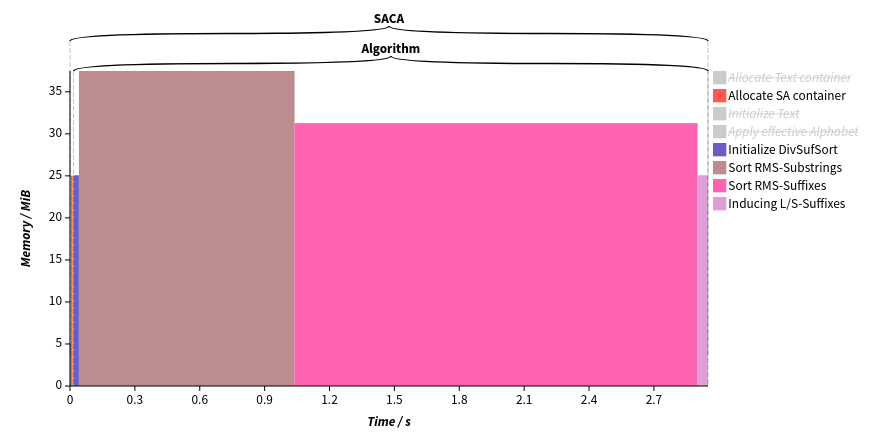
\includegraphics[width=\textwidth]{kapitel/1_extended_abstract/tudostat_example.png}
    \caption{Example of runtime and memory consumption of the phases of DivSufSort, measured by \sacabench and visualized on the tudostat website~\cite{tudostat}.}
    \label{ea:phases}
\end{figure}

You can evaluate a single algorithm with the command \termfont{sacabench construct} followed by the desired SACA and a path to an input file.
To get a list of all available Algorithms, you can execute the command \termfont{sacabench list}.
This will output the names for all available SACAs.

While the algorithm is running, its memory consumption is measured via the tudostat library~\cite{tudostat}.
You can also enable checking of the resulting suffix array with a fast suffix array checker~\cite{saca:11} by
using the \termfont{-c} or a parrallel version with the \termfont{-q} flag.
To generate a JSON file containing detailed information about the run of the selected Algorithm separated into SACA-specific phases,
the flag \termfont{-b} needs to be added to the command, followed by a destination path to which the report will be saved to.
To override an existing file at the destination path, the option \termfont{-f} can be used.
This file can be converted to a plot on the tudostat website~\cite{tudostat} (see Figure \ref{ea:phases} as an example).
If you add the flag \termfont{-{}-rplot}, a plot will be generated automatically after the SACA executed by using an R-script.
Additionally there is an alternative version of plots, which are generated using LaTex.
This can be done by adding the flag \termfont{-{}-latexplot}.

Multiple other flags and options allow to customize the way, the SACA is executed.
For example, it is possible to use a prefix of the given input string by adding \termfont{-p} together with the desired prefix size. 
This enables you to use one big input file for tests with a variety of input sizes.
Also it is possibile to execute the selected SACA multiple times on the same input and to combine the results.
This can be done by using the flag \termfont{-r} followed by the number of executions.
These and many more options are listed by the tool together with an explanation by adding \termfont{-h} to any subcommand.
An example would be:

\termfont{sacabench/sacabench construct -c -b /destination/path/to/result.json -f -p 1K -r 2 -{}-rplot -{}-latexplot BPR /path/to/input}

This command executes the SACA BPR two times on a prefix of the input file of 1 KB, 
uses the checker to validate the result and writes the resulting JSON file to the given path.
If there already is a file with the given name, it would be replaced by the new file.
After the SACA finished, plots are generated with both possible options.
To reduce the number of options, you can define them in a config file in INI format.
This configuration can be used by adding the flag \termfont{-{}-config} together with the path to the file.
An example of such a configuration can be seen in \ref{sacabench-construct:config:engl}.
Using the shown file, the command 

\termfont{sacabench/sacabench construct -{}-config /path/to/config BPR /path/to/input}

is the same as the previous command.

\begin{figure}[!h]
\begin{minted}
[
frame=lines,
framesep=2mm,
baselinestretch=1.2,
fontsize=\footnotesize,
linenos,
numbersep=-4mm,
breaklines,
escapeinside=@@,
frame=single,
framesep=14pt
]
{text}
check = true
benchmark = /destination/path/to/result.json
force = true
prefix = 1K
repetitions = 2
rplot = true
latexplot = true
\end{minted}
\caption{Example for a config file for command \texttt{sacabench construct}}
\label{sacabench-construct:config:engl}
\end{figure}

\subsection{Comparing multiple algorithms}

In order to compare different SACAs with each other, you can run a set of algorithms on a given input file.
This is achieved by using the \termfont{sacabench batch} command.
Most of the options available for the command \termfont{sacabench construct} are also valid for this command.
By default all included algorithms are run, but you can either deselect certain
algorithm with the \termfont{-{}-blacklist <saca name>} flag or run only certain
algorithms by using the \termfont{-{}-whitelist <saca name>} command.
These two options can also be added to the configuration file, as seen in the previous section.
The selected algorithms are run sequentially on the input text and their memory consumption
and construction times measured.
We also supply tools to convert the resulting JSON file into several types of plots, like bar plots, strong- and weak-scaling plots.
These plots differ from the ones created by \termfont{sacabench construct}.
They put the focus on comparing multiple algorithm against each other, instead of providing detailed information about the phases of the executed SACAs.
These plots can be used to compare the algorithms fairly.

\subsection{Adding additional SACAs}

A standardized interface for SACAs allows to easily add new implementations. Implementing this interface requires attributes for the name and a description of the SACA in order to be used via our commandline tool. Additionally the attribute for extra sentinels specifies, how many sentinels are added at the end of the input text by our framework, aiding in a more simple handling of corner cases. The realization of the corresponding member function represents the specified SACA, containing the added algorithm to correctly compute the \sa. Registering the SACA within our framework allows \sacabench to access the provided implementation, giving access to all features of our benchmark tool for the added algorithm.
See the \emph{README} in our GitHub repository~\cite{sacabench:github} for the detailed specification of our interface.
\section{SACA Overview}

There are many SACAs that operate using different principles.
The most na\"ive SACA uses a general purpose sorting algorithm to sort the suffixes of the input text.
Since a string comparison is $\mathcal O (n)$ in the worst-case, this would give $\mathcal O (n^2 \log n)$ runtime.
Even though this is a sub-optimal time bound,
there are several algorithms\footnote{e.g. Deep-Shallow, mSufSort, ...} in SACABench which don't improve on this
but rather use methods to speed up the real-world performance.
These methods can be classified into the categories \emph{inducing} and \emph{doubling}:
%
\paragraph{Inducing} %
There are different methods of inducing but they mostly operate by similar principles.
When the rank of a suffix $i$ (that is the position of $i$ in the \sa) is known,
it is possible to deduce the rank of other suffixes $j$.

The easiest to understand usecase for this is when using buckets.
Recall that a bucket $\mathsf b_{\sigma}$ is a region of the suffix
array which contains only and all the suffixes,
which start with the substring $\sigma$.
It is obvious that all the subbuckets $\mathsf b_{\sigma\alpha}$ for
every $\alpha \in \Sigma$ are contained within $\mathsf b_\sigma$.
It is possible to \emph{induce} the order of the $\mathsf b_{\alpha\sigma}$ bucket,
if all Buckets $\mathsf b_\sigma$ for every possible $\sigma \in \Sigma$ are already sorted (by whatever method),
since you know the regions of $\mathsf b_\alpha$ that are the $\mathsf b_{\alpha\sigma}$ Subbuckets.
You can then (for $\sigma \in \Sigma$) find the suffixes of $\mathsf b_{\alpha\sigma}$ in $\mathsf b_{\sigma}$,
subtract one of every index and write the found suffixes in-order to $\mathsf b_{\alpha\sigma}$.
Since the suffixes of $\mathsf b_{\alpha\sigma}$ are essentially the same as $\mathsf b_\sigma$ but
with only one (the same) character added in front of them,
their relative ordering is the same as the suffixes in $\mathsf b_\sigma$.
This method is used in e.g. Deep-Shallow~\cite{saca:4} and 
Bucket Pointer Refinement~\cite{saca:2}.

Another method of induction relies on the property of L- and S-Type suffixes and
is most prominently used in the SAIS algorithm~\cite{saca:6}.
This algorithm is based on sorting the LMS suffixes by recursion
and inducing the L-Type suffixes in a Left-to-right-pass and the S-type suffixes in a Right-to-Left-pass.
It can be shown that these steps result in a correct suffix array.

\paragraph{Doubling} Another fundamentally different approach to suffix sorting
aims to double the length of sorted suffixes in every iteration.
This is done by first sorting the suffixes by their first character only.
To then deduce the ordering of all the elements in the $\mathsf b_\alpha$ bucket,
one can look at the relative ordering of the suffixes that start one position
after the to-be-sorted suffix:
their relative ordering decide the ordering of the original suffixes.
In the next iteration one can look at the suffixes that start two positions later in the text,
and so on.
After $\mathcal O(\log n)$ iterations (since we double the prefix size in every iteration),
all the suffixes are sorted.
This method is used by qSufSort~\cite{saca:1} and the
doubling/discarding algorithm originally developed for use with external memory~\cite{saca:11}.

\bigskip\tableofcontents

\chapter{Einleitung}

Im \currentauthor{Christopher Poeplau und Marvin Böcker} Zuge der Projektgruppe 2018/2019 beschäftigt sich
\emph{SACABench} mit Suffix-Array-Konstruktions-Algorithmen. \emph{SACA} ist das Akronym für
\textbf{S}uffix \textbf{A}rray \textbf{C}onstruction \textbf{A}lgorithm und \emph{Bench} die Abkürzung für Benchmark,
also dem Messen von Laufzeit und Speicherplatz der Algorithmen.

Die Forschung an effizienten Konstruktionsalgorithmen für Suffix-Arrays hat in den letzten Jahren durch die
immer komplexer werdenden Anwendungen enorm an Bedeutung gewonnen. Gerade in der Bioinformatik,
in der man es im Bereich der Genomforschung mit Größenordnungen von Milliarden von Zeichen zu tun hat,
sind effiziente Algorithmen in Bezug auf Zeit und Speicherplatz notwendig~\cite[ch.~1]{saca:6}.

Ein Suffix-Array repräsentiert die Suffixe eines Strings $T$ in lexikographischer Reihenfolge.
Sei $T=suffix$. Für den String $T$ ergibt sich die folgende Suffix-Tabelle:
%
\begin{center}
  \begin{tabular}{ | l | c | r }
    \hline
        $i$ & $T[i, n)$ \\ \hline
        0 & suffix \\ \hline
        1 & uffix \\ \hline
        2 & ffix \\ \hline
        3 & fix \\ \hline
        4 & ix \\ \hline
        5 & x \\ \hline
        6 & \$ \\
    \hline
  \end{tabular}
\end{center}
%
Es ist sofort ersichtlich, dass $T[0, n) = T$ und $T[n-2, n)=\$$ gilt.
Sortiert man die Suffixe nun lexikografisch, ergibt sich das Suffix-Array:
%
\begin{center}
  \begin{tabular}{ | l | c | r }
    \hline
        $i$ & $T[i, n)$ \\ \hline
        6 & \$ \\ \hline
        3 & fix \\ \hline
        2 & ffix \\ \hline
        4 & ix \\ \hline
        0 & suffix \\ \hline
        1 & uffix \\ \hline
        5 & x \\
    \hline
  \end{tabular}
\end{center}
%
Somit ergibt sich als Suffix-Array $SA(T)$: $\{6,3,2,4,0,1,5\}$

Ziel ist die effiziente Konstruktion dieses Arrays.
Dabei gibt es Algorithmen, die den Fokus auf die Laufzeit setzen,
andere wiederum auf die Speicheroptimierung und wieder andere versuchen den besten Kompromiss aus beiden Welten zu finden.
Die Aufgabe der Projektgruppe ist das Schaffen einer umfangreichen Library der bekanntesten SACAs,
eingebettet in ein Framework, das es ermöglicht auf intuitiver Art und Weise Algorithmen auf beliebigen
Texten zu testen und die Performance miteinander zu vergleichen. Grundziel des Frameworks ist die Vereinheitlichung.
Viele der Algorithmen existieren in einzelnen Repositorys und die Algorithmen werden in den meisten Fällen 
nicht auf vergleichbarer Basis getestet und analysiert. Diese Algorithmen gilt es zunächst zu verstehen
und dann zu implementieren, sodass sie den Schnittstellen des Frameworks genügen.
Es soll also ein erweiterbares Gesamtkonstrukt geschaffen werden, das bestehende SACAs
sammelt und repräsentatives Vergleichen der Algorithmen ermöglicht.

\section{Notation und Definitionen}
\todo{Macht die Definitionen lieber wirklich als Definitionen und nicht als subsections}
Einige\currentauthor{Rosa Pink und\\Marvin Löbel} grundlegende Notationen und Definitionen werden hier kurz vorangestellt.

\begin{definition}[Intervall]
Wir nutzen $[i, j] = \{i, \dots, j\}$ und $[i, j) = [i, j - 1]$ als Kurzschreibweise für Integer-Intervalle.
\end{definition}

\begin{definition}[Alphabet und lexikographische Sortierung]
Das konstante Alphabet ist definiert als $\Sigma = \{\sigma_1, \sigma_2, ..., \sigma_{|\Sigma|-1}\} \cup \{\$\}$.
Es besteht aus Symbolen bzw. Zeichen $\sigma_i$, die im Eingabe-String vorkommen dürfen, und dem Sentinel-Symbol \$, welches das Ende des Strings markiert. 
Die Zeichen sind wie folgt lexikographisch (nach \textit{lexikographischer Sortierung})
geordnet: $\$ < \sigma_1 < \sigma_2 < ... < \sigma_{|\Sigma|-1}$. 
Sie lassen sich durch Integer-Werte repräsentieren, indem wir \$ den Wert 0 zuweisen und $\sigma_i$ den Wert $i$.
$\Sigma^+$ bezeichnet weiter die Menge aller Strings über diesem Alphabet mit echt positiver Länge.
\end{definition}

\begin{definition}[Input-String und Suffix]
Der Input-String wird \inputtext genannt und hat die Länge $n$. Das $i$-te Zeichen im
Input-String ist \inputtext[i], das $i$-te Suffix  (kurz: Suffix $i$) ist 
\begin{align*}
\suffix{i} := \inputtext[i,n) = \inputtext[i]\inputtext[i+1]...\inputtext[n-1]
\end{align*} \inputtext[n]
ist das Terminalsymbol \$ (sowie alle \inputtext[m] mit $m>n$) und ist formal nicht Teil des Eingabe-Strings.
Der Eingabe-String beginnt bei \inputtext[0].
\end{definition}

\begin{definition}[Suffix-Array]
Das Suffix-Array, kurz \sa, bezeichnet ein Array, in dem in lexikographischer Reihenfolge
die Suffix-Indizes (Positionen des Anfangsbuchstabens) gespeichert sind.
Das bedeutet, $\sa[j] = i$ genau dann, wenn $\mathsf{T}[i,n)$ das $j$-te Suffix von \inputtext in lexikografischer Ordnung ist.
\end{definition}

\begin{definition}[Bucket]
    \label{def:bucket}
    Alle Suffixe, die mit demselben Zeichen $c_0 \in \Sigma$ beginnen, formen ein zusammenhängendes Intervall im Suffix-Array.
    Dieses Intervall wird $c_0$-Bucket genannt und mit $\bucket{c_0}$ bezeichnet.
    Der $(c_0,c_1)$-Bucket $\bucket{c_0, c_1}$ bezeichnet das Intervall, dessen Suffixe mit denselben zwei Zeichen $c_0, c_1 \in \Sigma$ beginnen.\par
    Ähnlich dazu bezeichnet der Bucket $\bucket{\omega}$ alle Suffixe im \sa, die alle mit dem String $\omega \in \Sigma^m$ mit \(m > 0\) anfangen. \(\bucket{\omega}\) heißt dann auch Level-\(m\)-Bucket.
\end{definition}

\begin{definition}[Textwiederholung]
\label{def:repetition}
Eine Wiederholung in $\mathsf{T}$ ist ein Teilstring $\mathsf{T}[i, i + rp]$ mit $ r \geq 2, p \geq 0$ und $i, i + rp \in [0, n)$, sodass $\mathsf{T}[i, i+p) = \mathsf{T}[i + p, i + 2p) = \dots = \mathsf{T}[i + (r-1)p, i + rp)$.
\end{definition}

\subsection{Praxisrelevante Grenzen}

Wir gehen im Folgenden davon aus, dass für unsere Eingabe $|\Sigma| = 256$ gilt, da sich so jedes Zeichen durch ein Byte repräsentieren lässt. Dies erlaubt auch das direkte Verarbeiten von Texten in Standardkodierungen wie ASCII und UTF-8~\cite{grundlagen:utf8}, die durch Byte-Arrays ohne 0-Bytes repräsentiert werden.

Auch gehen wir davon aus, das die Länge $n$ von Datenstrukturen, insbesondere der Eingabe und des Suffix-Arrays, durch die maximale Größe nativer Integer-Datentypen in Consumer-Computersystemen begrenzt ist. Es gilt somit in der Regel $n \leq 2^{32}$ oder $n \leq 2^{64}$, womit sich Indizes durch 4- bzw. 8-Byte Integer repräsentieren lassen. Wir betrachten außerdem $n = 2^{40}$ als 5-Byte Kompromiss zwischen den Beiden.

\subsection{Codebeispiele}

Wir geben alle algorithmischen Codebeispiele in an Python angelehnten Pseudocode an.

%\section{Notationen und Definitionen}
%\label{definitions}
%Sei \currentauthor{Christopher Poeplau} $T$ ein Text mit Zeichenanzahl $\vert T \vert = n$
%\begin{itemize}
%    \item $\Sigma (T)$ := Alphabet von $T$
%    \item Ein Substring von $T[i, j) = T[i]...T[j-1]$
%    \item $T$ wird durch das lexikografisch kleinste Zeichen, dem $\$$ terminiert (engl. sentinel)
%\end{itemize} 
%\bigskip
%Suffix $S_i=T[i,n)$ als das in $i$ beginnende Suffix in $T$. 
%\begin{itemize}
%    \item Das Suffix ist ein S(hort)-Type-Suffix $\iff S_i<S_{i+1}$
%    \item Das Suffix ist ein L(arge)-Type-Suffix $\iff S_i>S_{i+1}$
%    \item $Type('\$') := S$
%    \item Ein Zeichen $T[i]$ ist S-Type $\iff Type(S_i) = S$
%    \item Ein Zeichen $T[i]$ ist L-Type $\iff Type(S_i) = L$
%\end{itemize}
%
%\subsection{Leftmost S-Type}
%Ein Zeichen $T[i]$ des Strings $T$ ist genau dann LMS, wenn $Type(T[i-1])=L$, also das Vorgängerzeichen vom Typ $L$ ist. Gleichzeitig ist ein Suffix $T[i, n)$ ein LMS-Suffix, wenn $T[i]$ LMS ist.\\
%Ein Substring $T[i, j]$, $i\neq j$, ist LMS, wenn $Type(T[i])=S$ und $Type(T[j])=S$. Zudem darf in diesem Substring kein weiteres LMS-Zeichen vorhanden sein. Insbesondere ist $T[j]$ dadurch exklusiv und gehört nicht zu dem Substring. \\
%Für die Gleichheit zweier LMS-Substrings gilt das folgende: \\
%Seien $T_1$ und $T_2$ LMS-Substrings.
%\begin{center}
%    $S_1=S_2 \iff \vert S_1 \vert = \vert S_2 \vert $ $\wedge$ $S_1$ besitzt dieselben Zeichen wie $S_2$ in derselben Reihenfolge
%\end{center}


\chapter{Framework}
Zur \currentauthor{Rosa Pink} Durchführung eines Benchmarks und allgemein zur besseren und leichteren Visualisierung von Laufzeit und Speicherverbrauch der Algorithmen haben wir ein Framework entwickelt. Unser Framework kann mit beliebigen Algorithmen für beliebige Eingaben Suffix-Arrays konstruieren und anschließend die Ergebnisse in der Konsole ausgeben oder ansprechende Graphiken daraus erzeugen.
\section{Command Line Interface}

Das \currentauthor{David Piper und\\ Florian Grieskamp} \sacabench-Framework wurde mit dem Ziel entworfen, alle enthaltenen Funktionen flexibel aufrufen sowie Ein- und Ausgaben mit UNIX-Tools einfach verarbeiten zu können.
Es können daher alle Komponenten über ein Command Line Interface (CLI) angesprochen werden, um Zugriff auf deren Funktionalitäten zu erlangen.
Das Hauptprogramm unterteilt sich in fünf Bestandteile:
\begin{description}
    \item[\termfont{sacabench list}] gibt eine Liste aller verfügbaren Implementierungen aus, welche neben den im Rahmen der Projektgruppe implementierten Algorithmen auch die zugehörigen Referenzimplementierungen beinhaltet.
        Alle Funktionen dieser Komponente werden in \cref{framework:cli:sacabench-list} genauer erklärt.
    \item[\termfont{sacabench demo}] führt alle enthaltenen Algorithmen auf einer Beispieleingabe aus, um deren Funktionalität zu demonstrieren.
        Alle Funktionen dieser Komponente werden in \cref{framework:cli:sacabench-demo} genauer erklärt.
    \item[\termfont{sacabench construct}] führt einen einzelnen Algorithmus wahlweise auf einer Eingabedatei oder auf der Standardeingabe aus und bietet unter anderem die Optionen, die Laufzeit der Verarbeitung zu messen oder die Korrektheit der Ausgabe zu testen. Alle Funktionen dieser Komponente werden in \cref{framework:cli:sacabench-construct} genauer erklärt.
    \item[\termfont{sacabench batch}] bietet ähnliche Funktionen wie \termfont{sacabench construct}, wendet aber mehrere Algorithmen auf den Eingabetext an. Dadurch kann die Effizienz ausgewählter Verfahren verglichen werden. Alle Funktionen dieser Komponente werden in \cref{framework:cli:sacabench-batch} genauer erklärt.
    \item[\termfont{sacabench plot}] ermöglicht es, zu einer zuvor bereits durchgeführte Messung PDF-Dateien zu generieren. Dieses Kommando ist in \cref{framework:cli:sacabench-plot} näher beschrieben.
\end{description}

\subsection{sacabench}
\label{framework:cli:sacabench}

{
\begin{wrapfigure}[16]{R}[5mm]{.5\textwidth}
    \vspace{-1.5\baselineskip}
    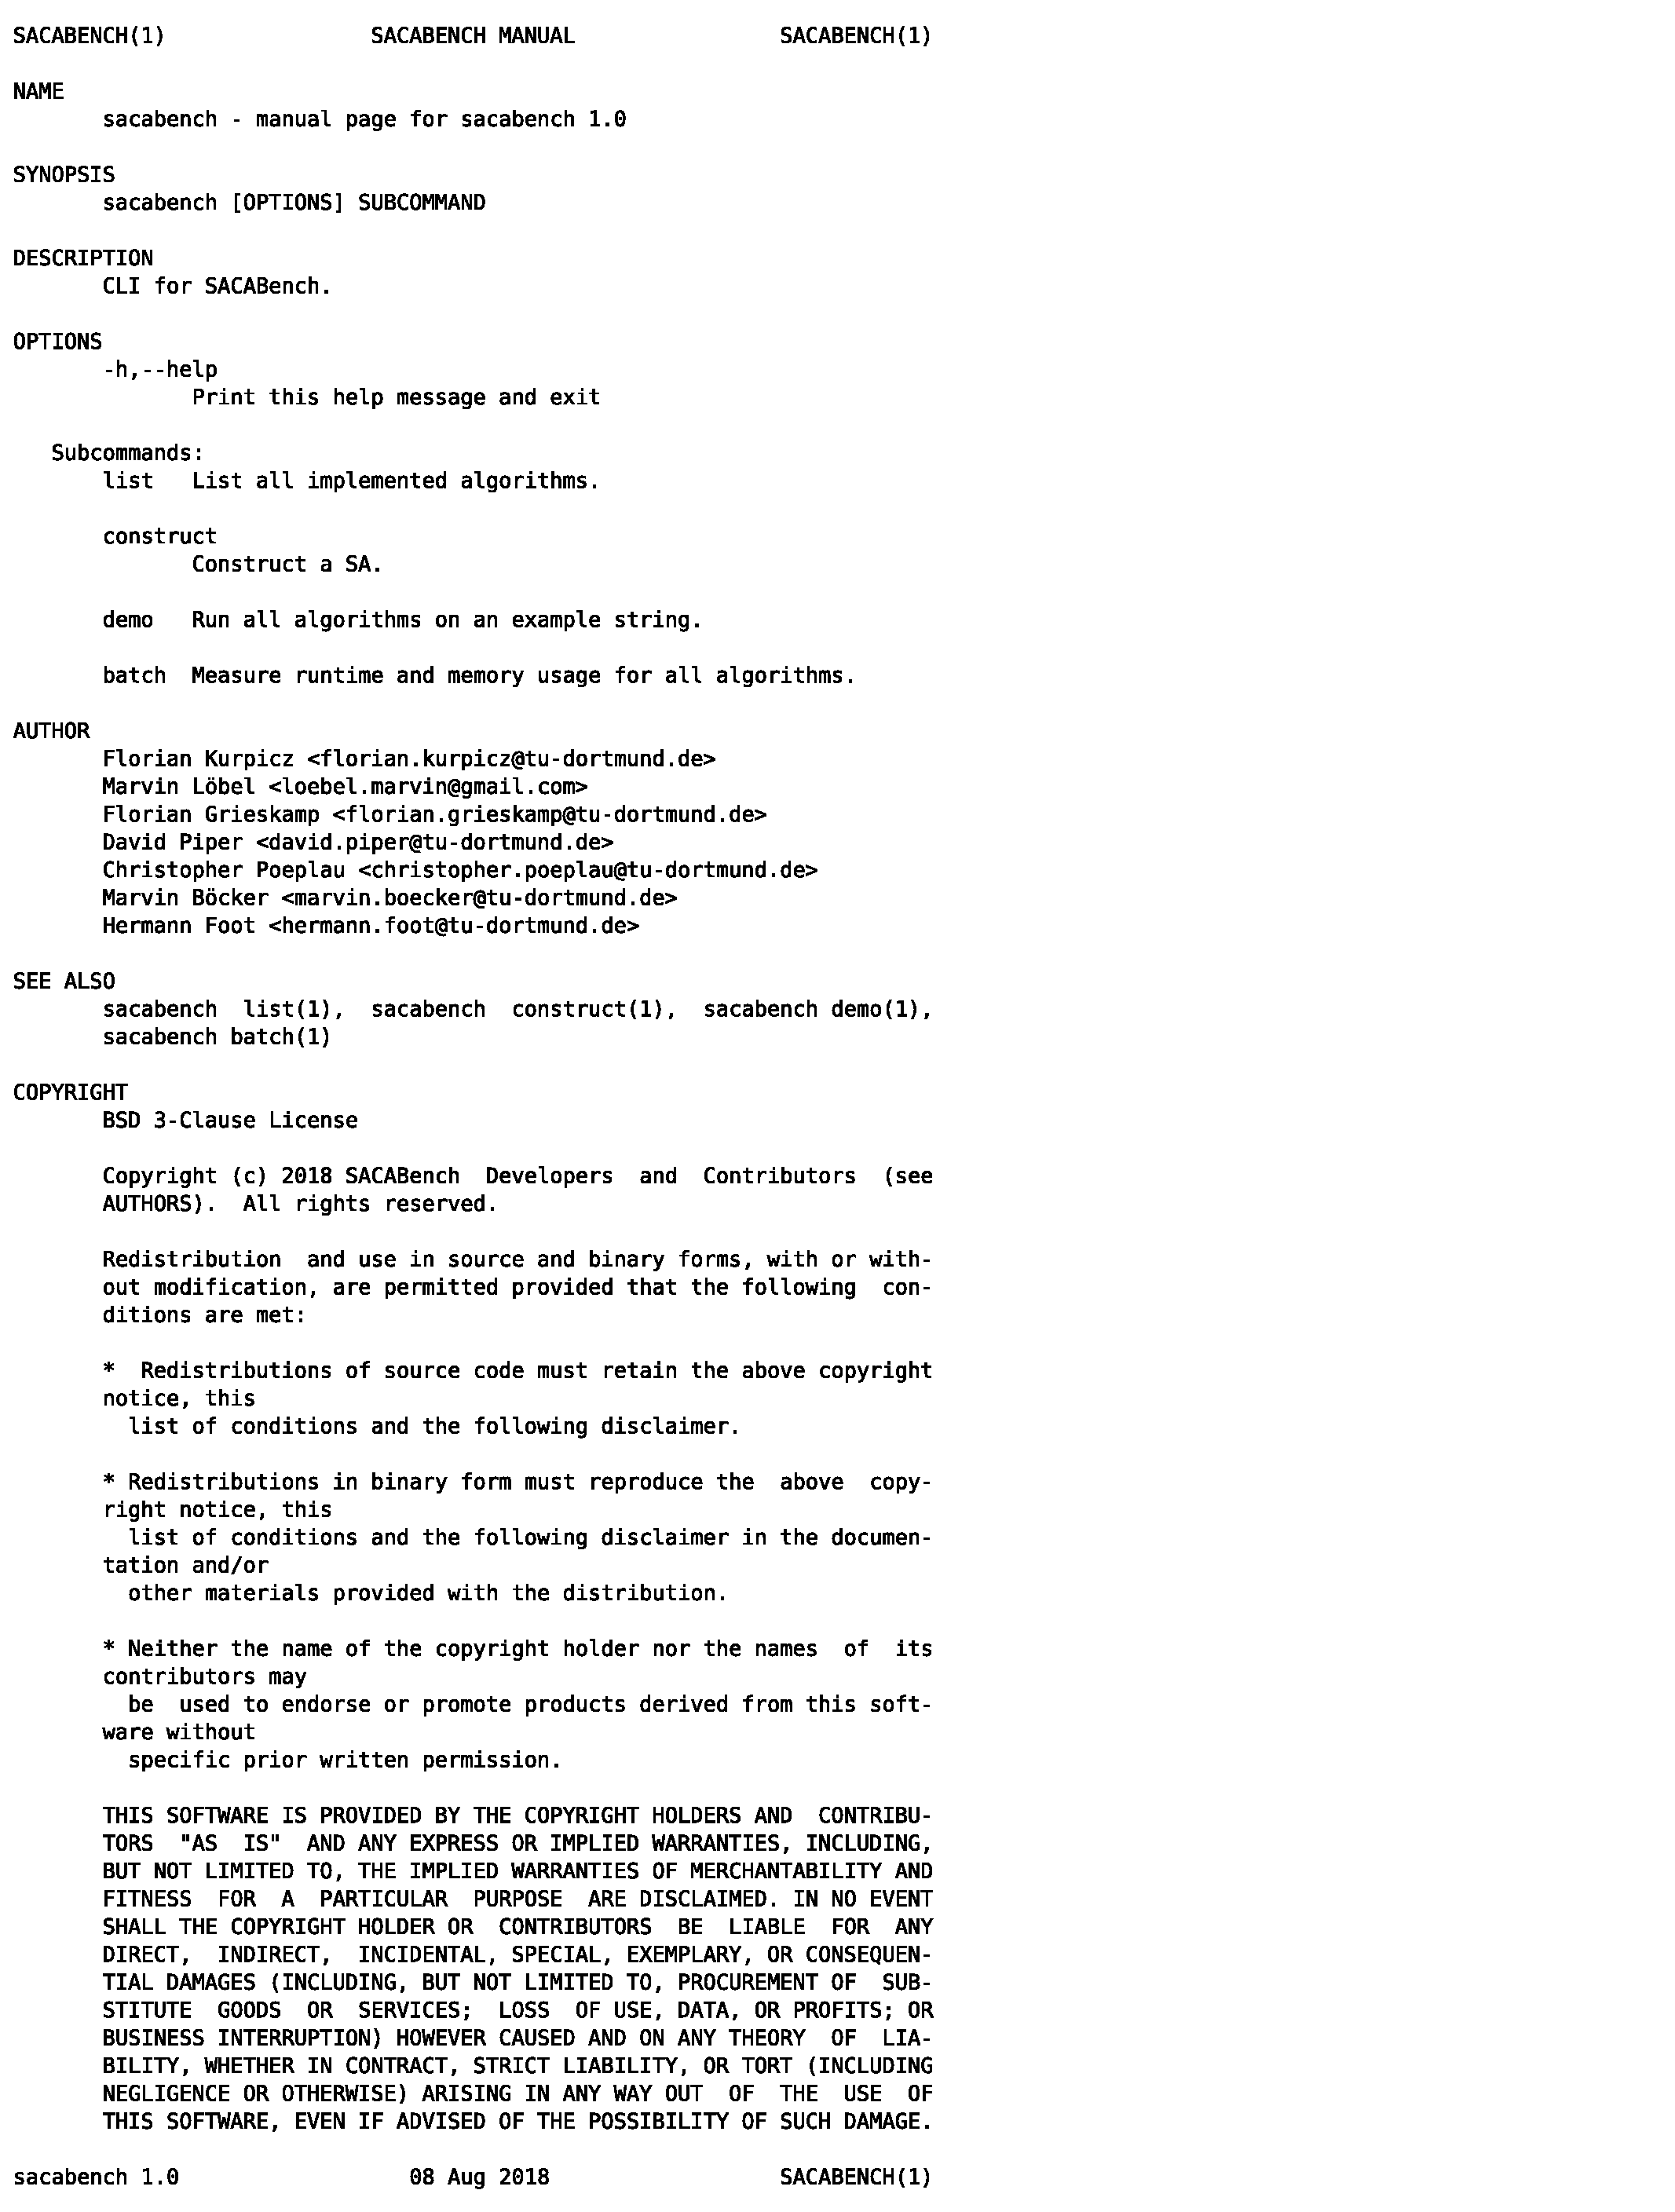
\includegraphics[page=1, viewport=0cm 32.8cm 20.5cm 47.5cm, clip, width=.5\textwidth]{{kapitel/3_framework/cli/sacabench/sacabench}.pdf}\\
    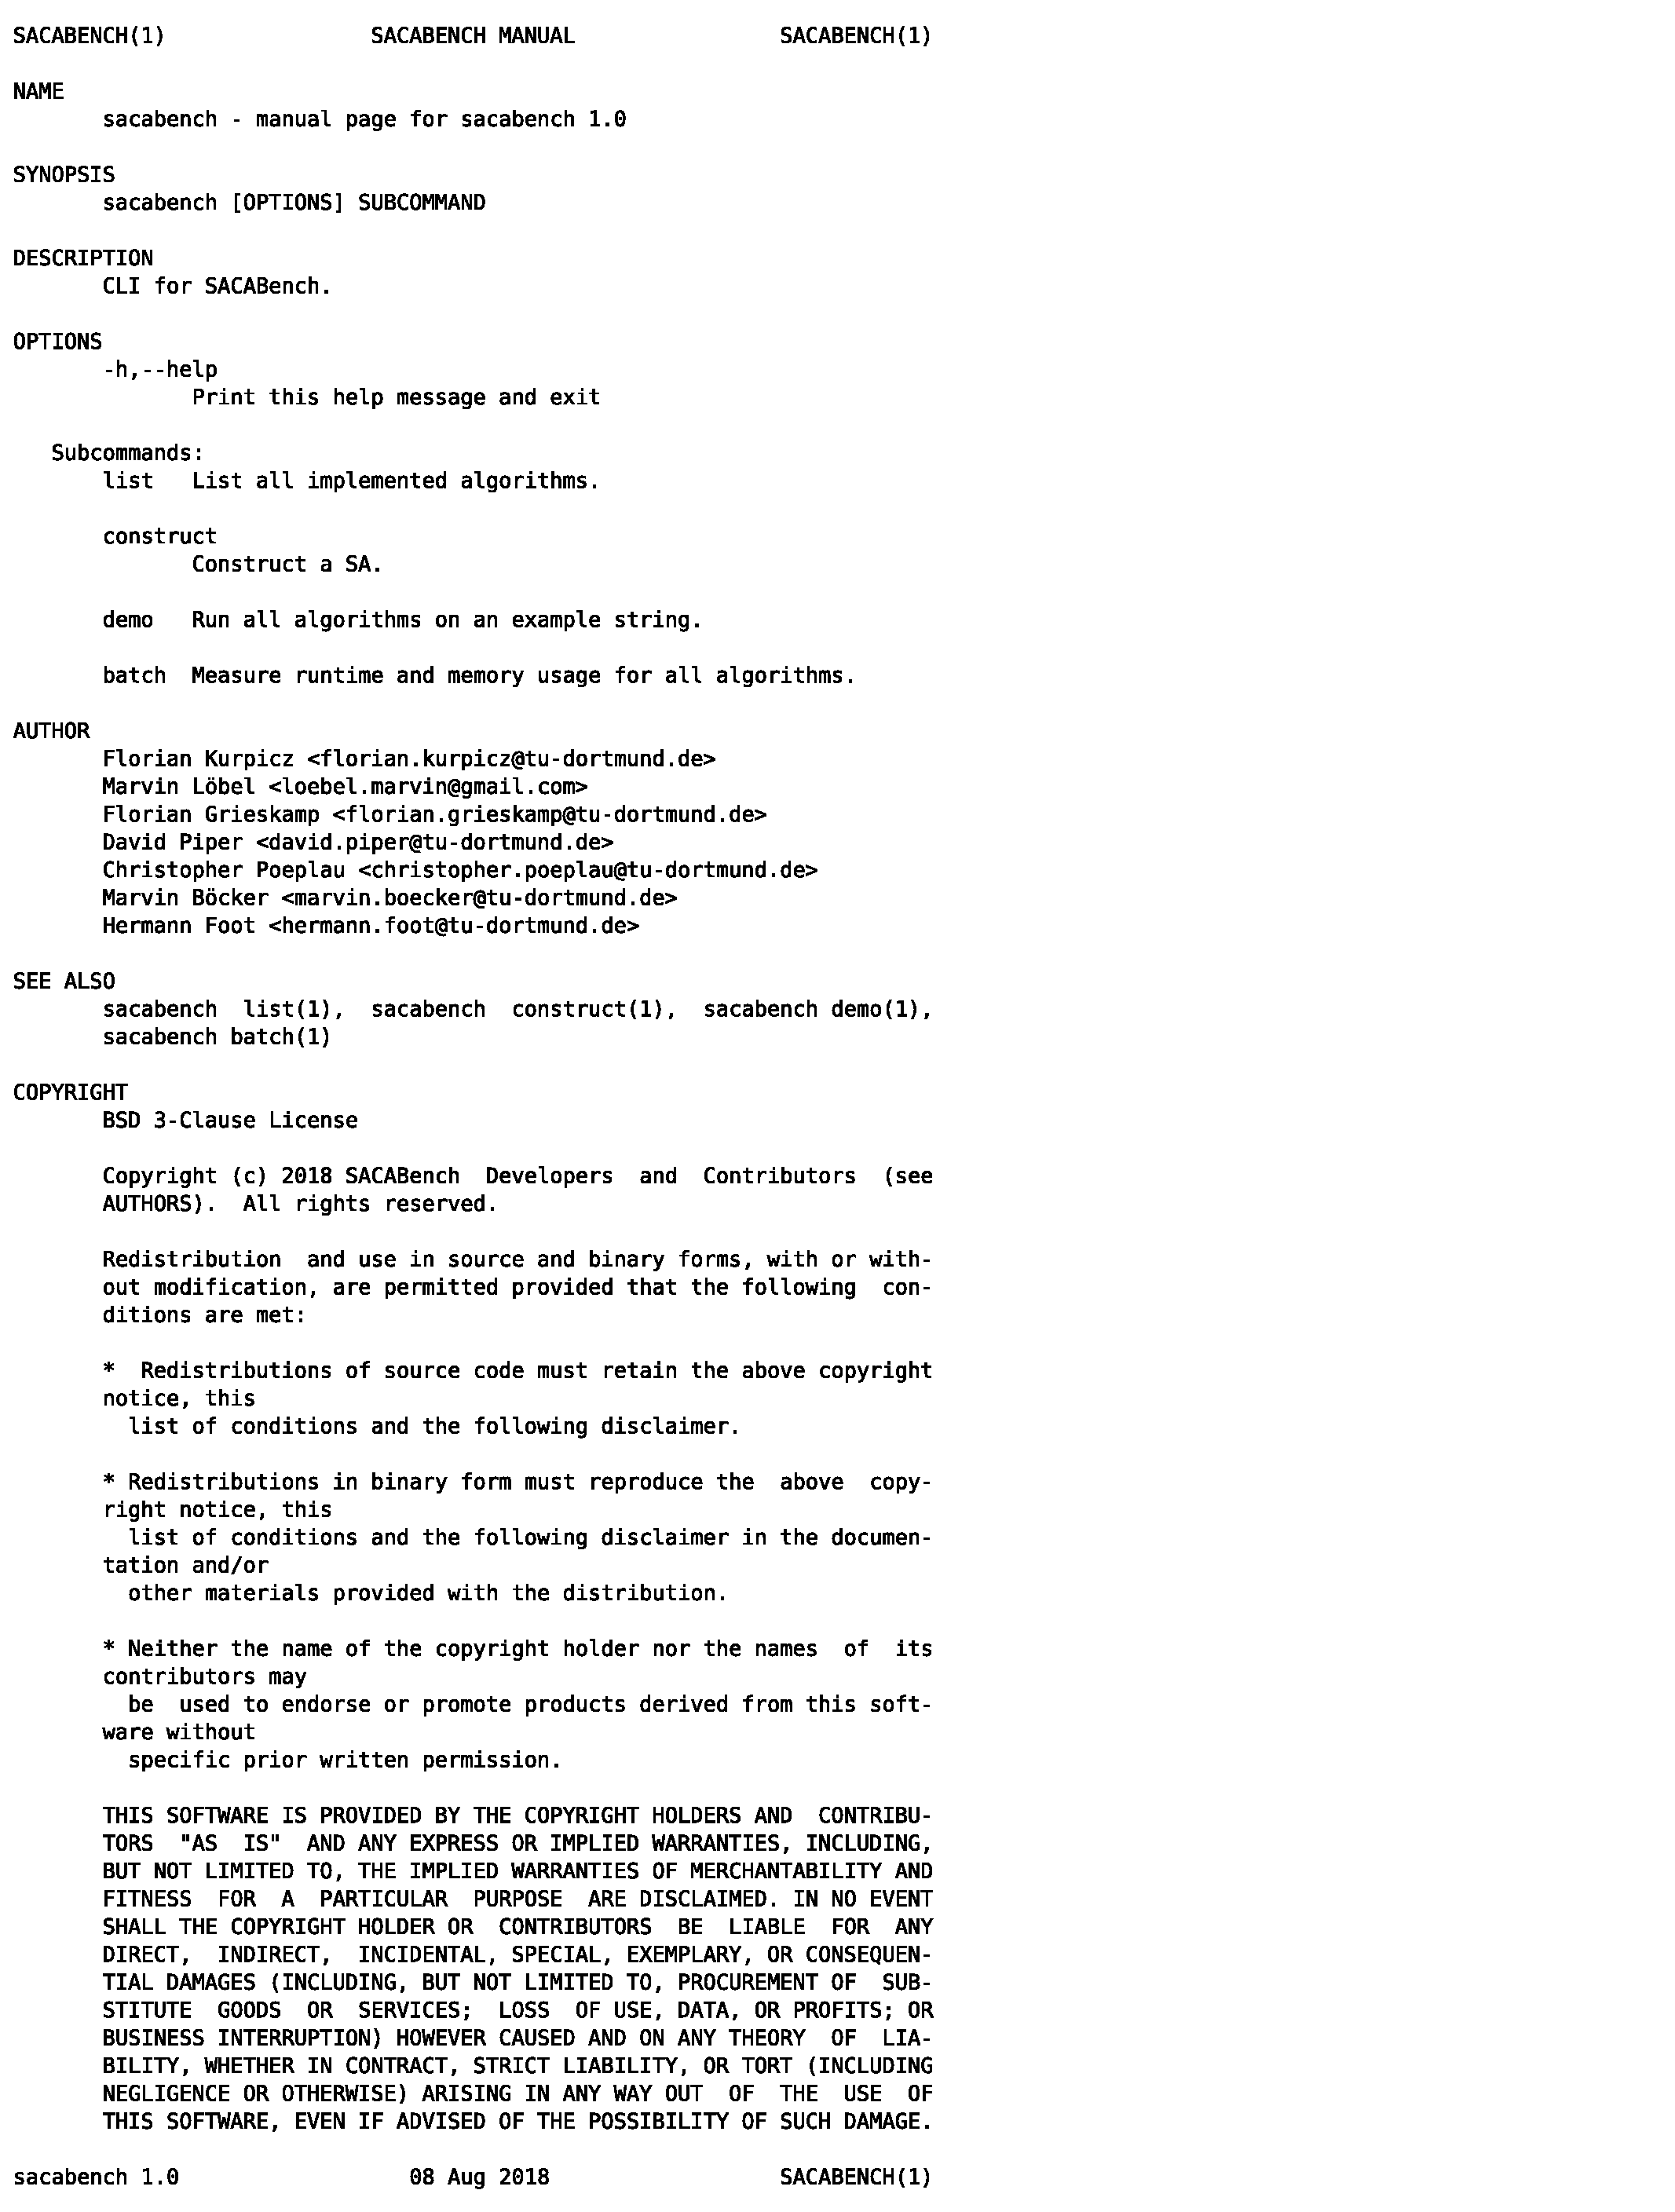
\includegraphics[page=1, viewport=0cm 25cm 20.5cm 27.3cm, clip, width=.5\textwidth]{{kapitel/3_framework/cli/sacabench/sacabench}.pdf}\\
    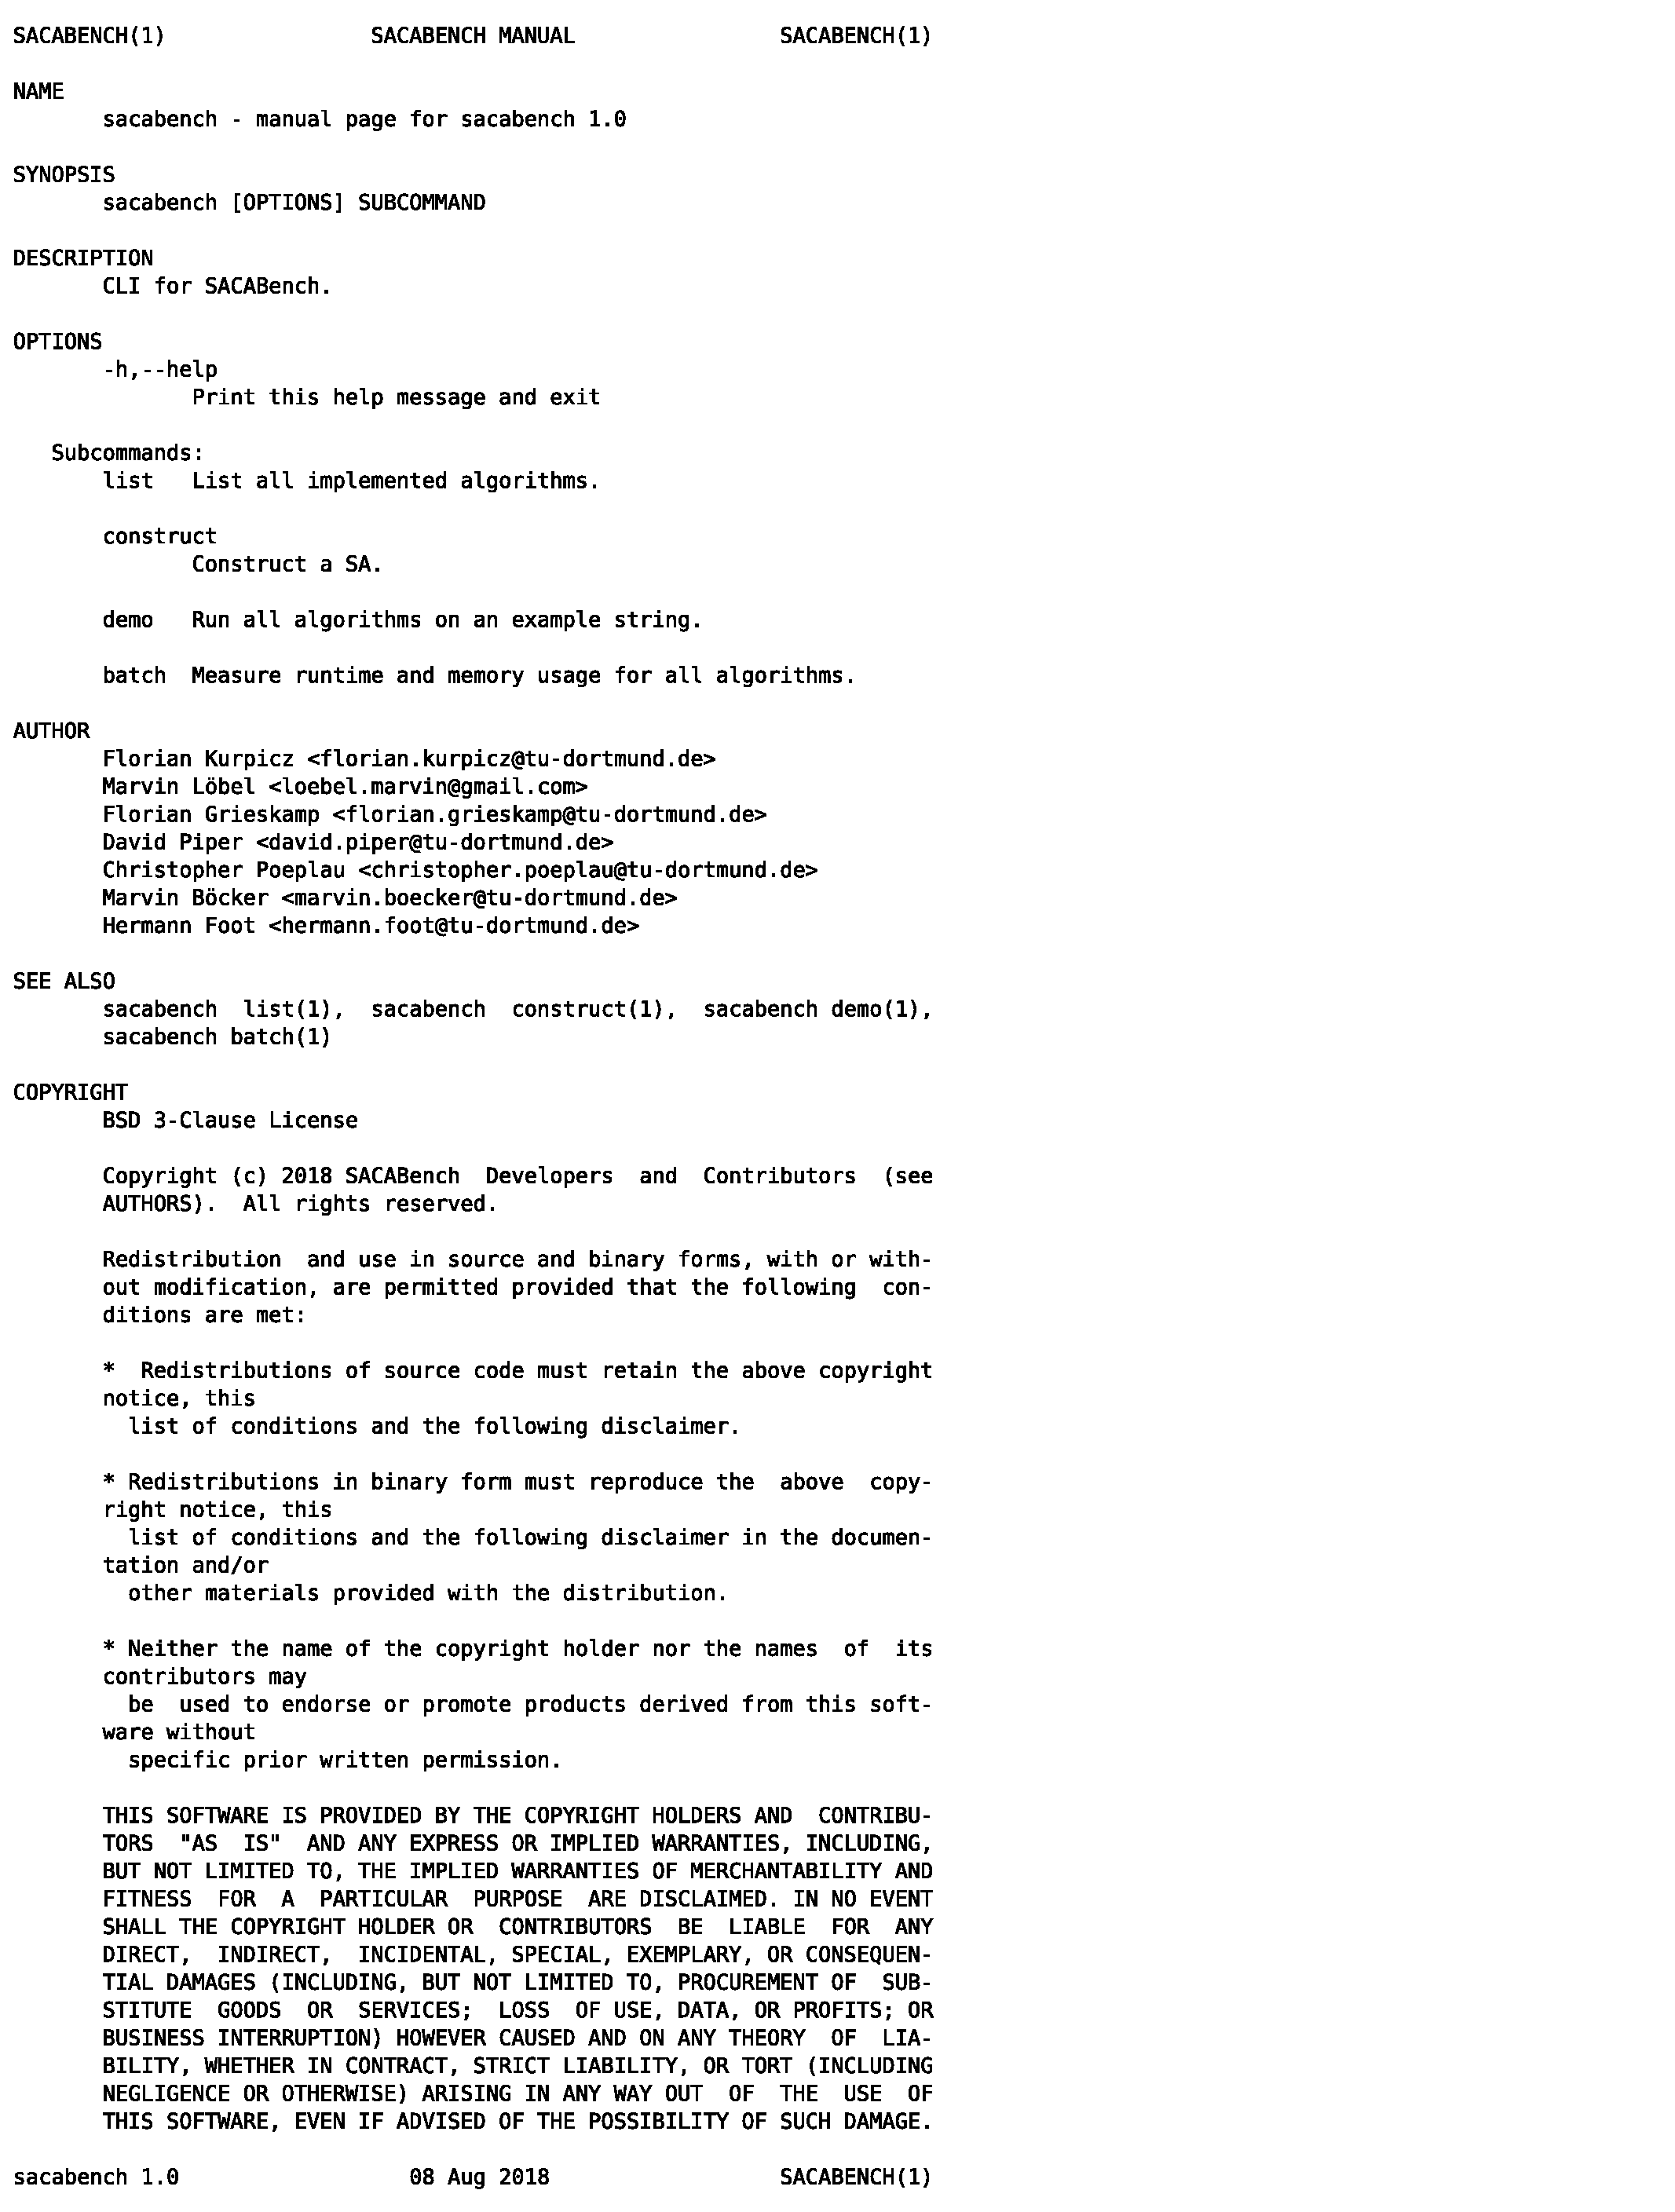
\includegraphics[page=1, viewport=0cm 0cm 20.5cm 1.5cm, clip, width=.5\textwidth]{{kapitel/3_framework/cli/sacabench/sacabench}.pdf}
    \caption{Gekürzte Ausgabe von \texttt{man sacabench}.}
    \label{manpage:sacabench}
\end{wrapfigure}
Das Hauptprogramm wird mit dem Befehl \texttt{sacabench} ausgeführt.
Für die einzelnen Funktionen stehen ent\-sprech\-ende Subcommands zur Verfügung.
Alle Komponenten beinhalten eine Hilfefunktion, die sich durch die Option \termfont{-h} bzw. \termfont{-{}-help} aufrufen lässt.
Die gleiche Hilfe wird außerdem ausgegeben, wenn das Programm mit ungültigen Parametern aufgerufen wird.
Für präzisere Erläuterungen der Aufrufe und Optionen stehen außerdem Man-Pages für alle Subcommands zur Verfügung.
Diese sind wie gewohnt über \termfont{man sacabench} bzw. \termfont{man sacabench [SUBCOMMAND]} aufzurufen und beinhalten neben der Beschreibung der Befehlssyntax und den Erläuterungen zur Verwendung der Optionen auch eine Liste der beteiligten Autoren, Verweise auf ähnliche Befehle und die Copyright-Bestimmungen.
Eine gekürzte Version der Man-Page für den Befehl \termfont{sacabench} ist in \cref{manpage:sacabench} zu sehen.
Alle im hier abgebildeten Man-Pages sind aus Gründen der Übersichtlichkeit um die Liste der Autoren und den Copyright-Verweis reduziert.\par
}

\subsection{sacabench list}
\label{framework:cli:sacabench-list}

Mit dem Befehl \texttt{sacabench list} können alle verfügbaren Algorithmen aufgelistet werden.
Nach dem Aufruf erscheint eine Liste aller im Rahmen der Projektgruppe implementierten Algorithmen, sowie deren Referenzimplementierungen. 
Letztere sind in der angegebenen Abkürzung durch \termfont{\_ref} markiert.\par
Über die Option \termfont{-{}-no-description} kann außerdem die Ausgabe der Kurz\-be\-schrei\-bungen unterdrückt werden, sodass nur noch eine Liste aller Kürzel erscheint. 
Die dort aufgelisteten Kürzel entsprechen den Bezeichnungen der Algorithmen, über die sie vom Framework referenziert werden.
Zusätzlich ermöglicht es die Option \termfont{-j} oder \termfont{-{}-json}, die Namen der Algorithmen als ein JSON Array auszugeben.\par

\subsection{sacabench demo}
\label{framework:cli:sacabench-demo}

{
\begin{wrapfigure}[9]{rR}[5mm]{.5\textwidth}
    \vspace{-1.5\baselineskip}
    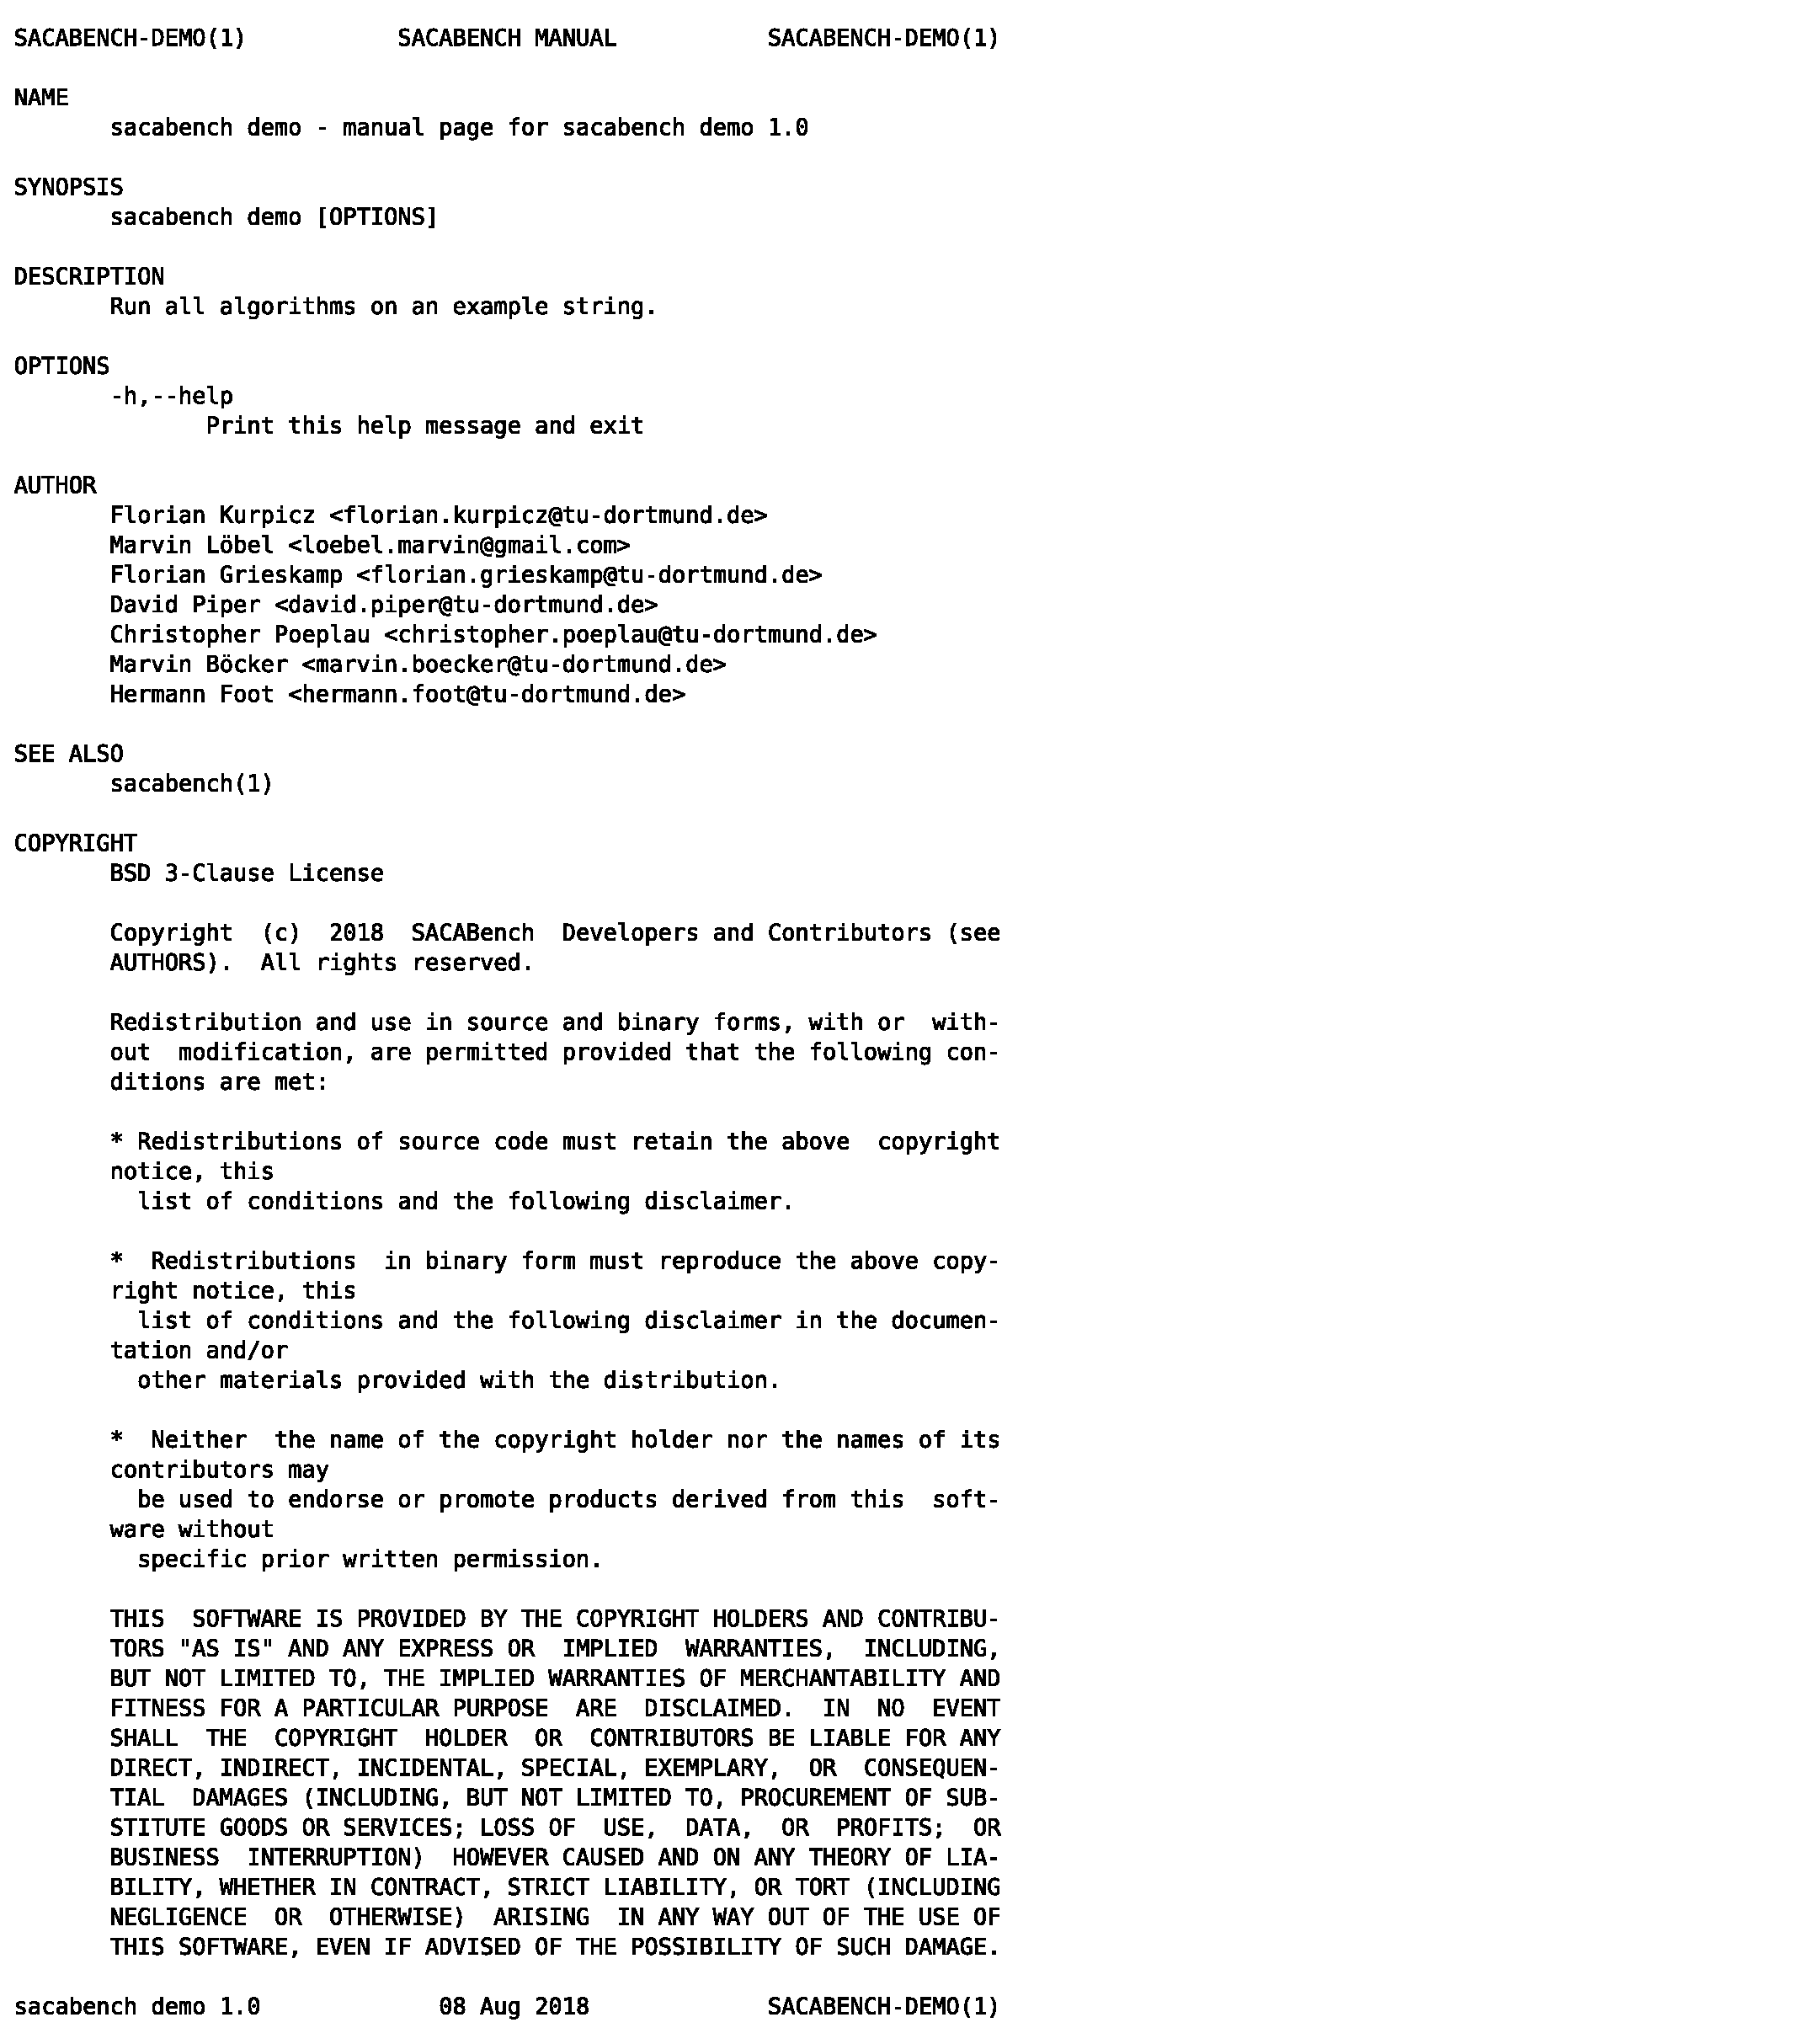
\includegraphics[page=1, viewport=0cm 32.8cm 20.5cm 41.0cm, clip, width=.5\textwidth]{{kapitel/3_framework/cli/sacabench-demo/sacabench-demo}.pdf}\\
    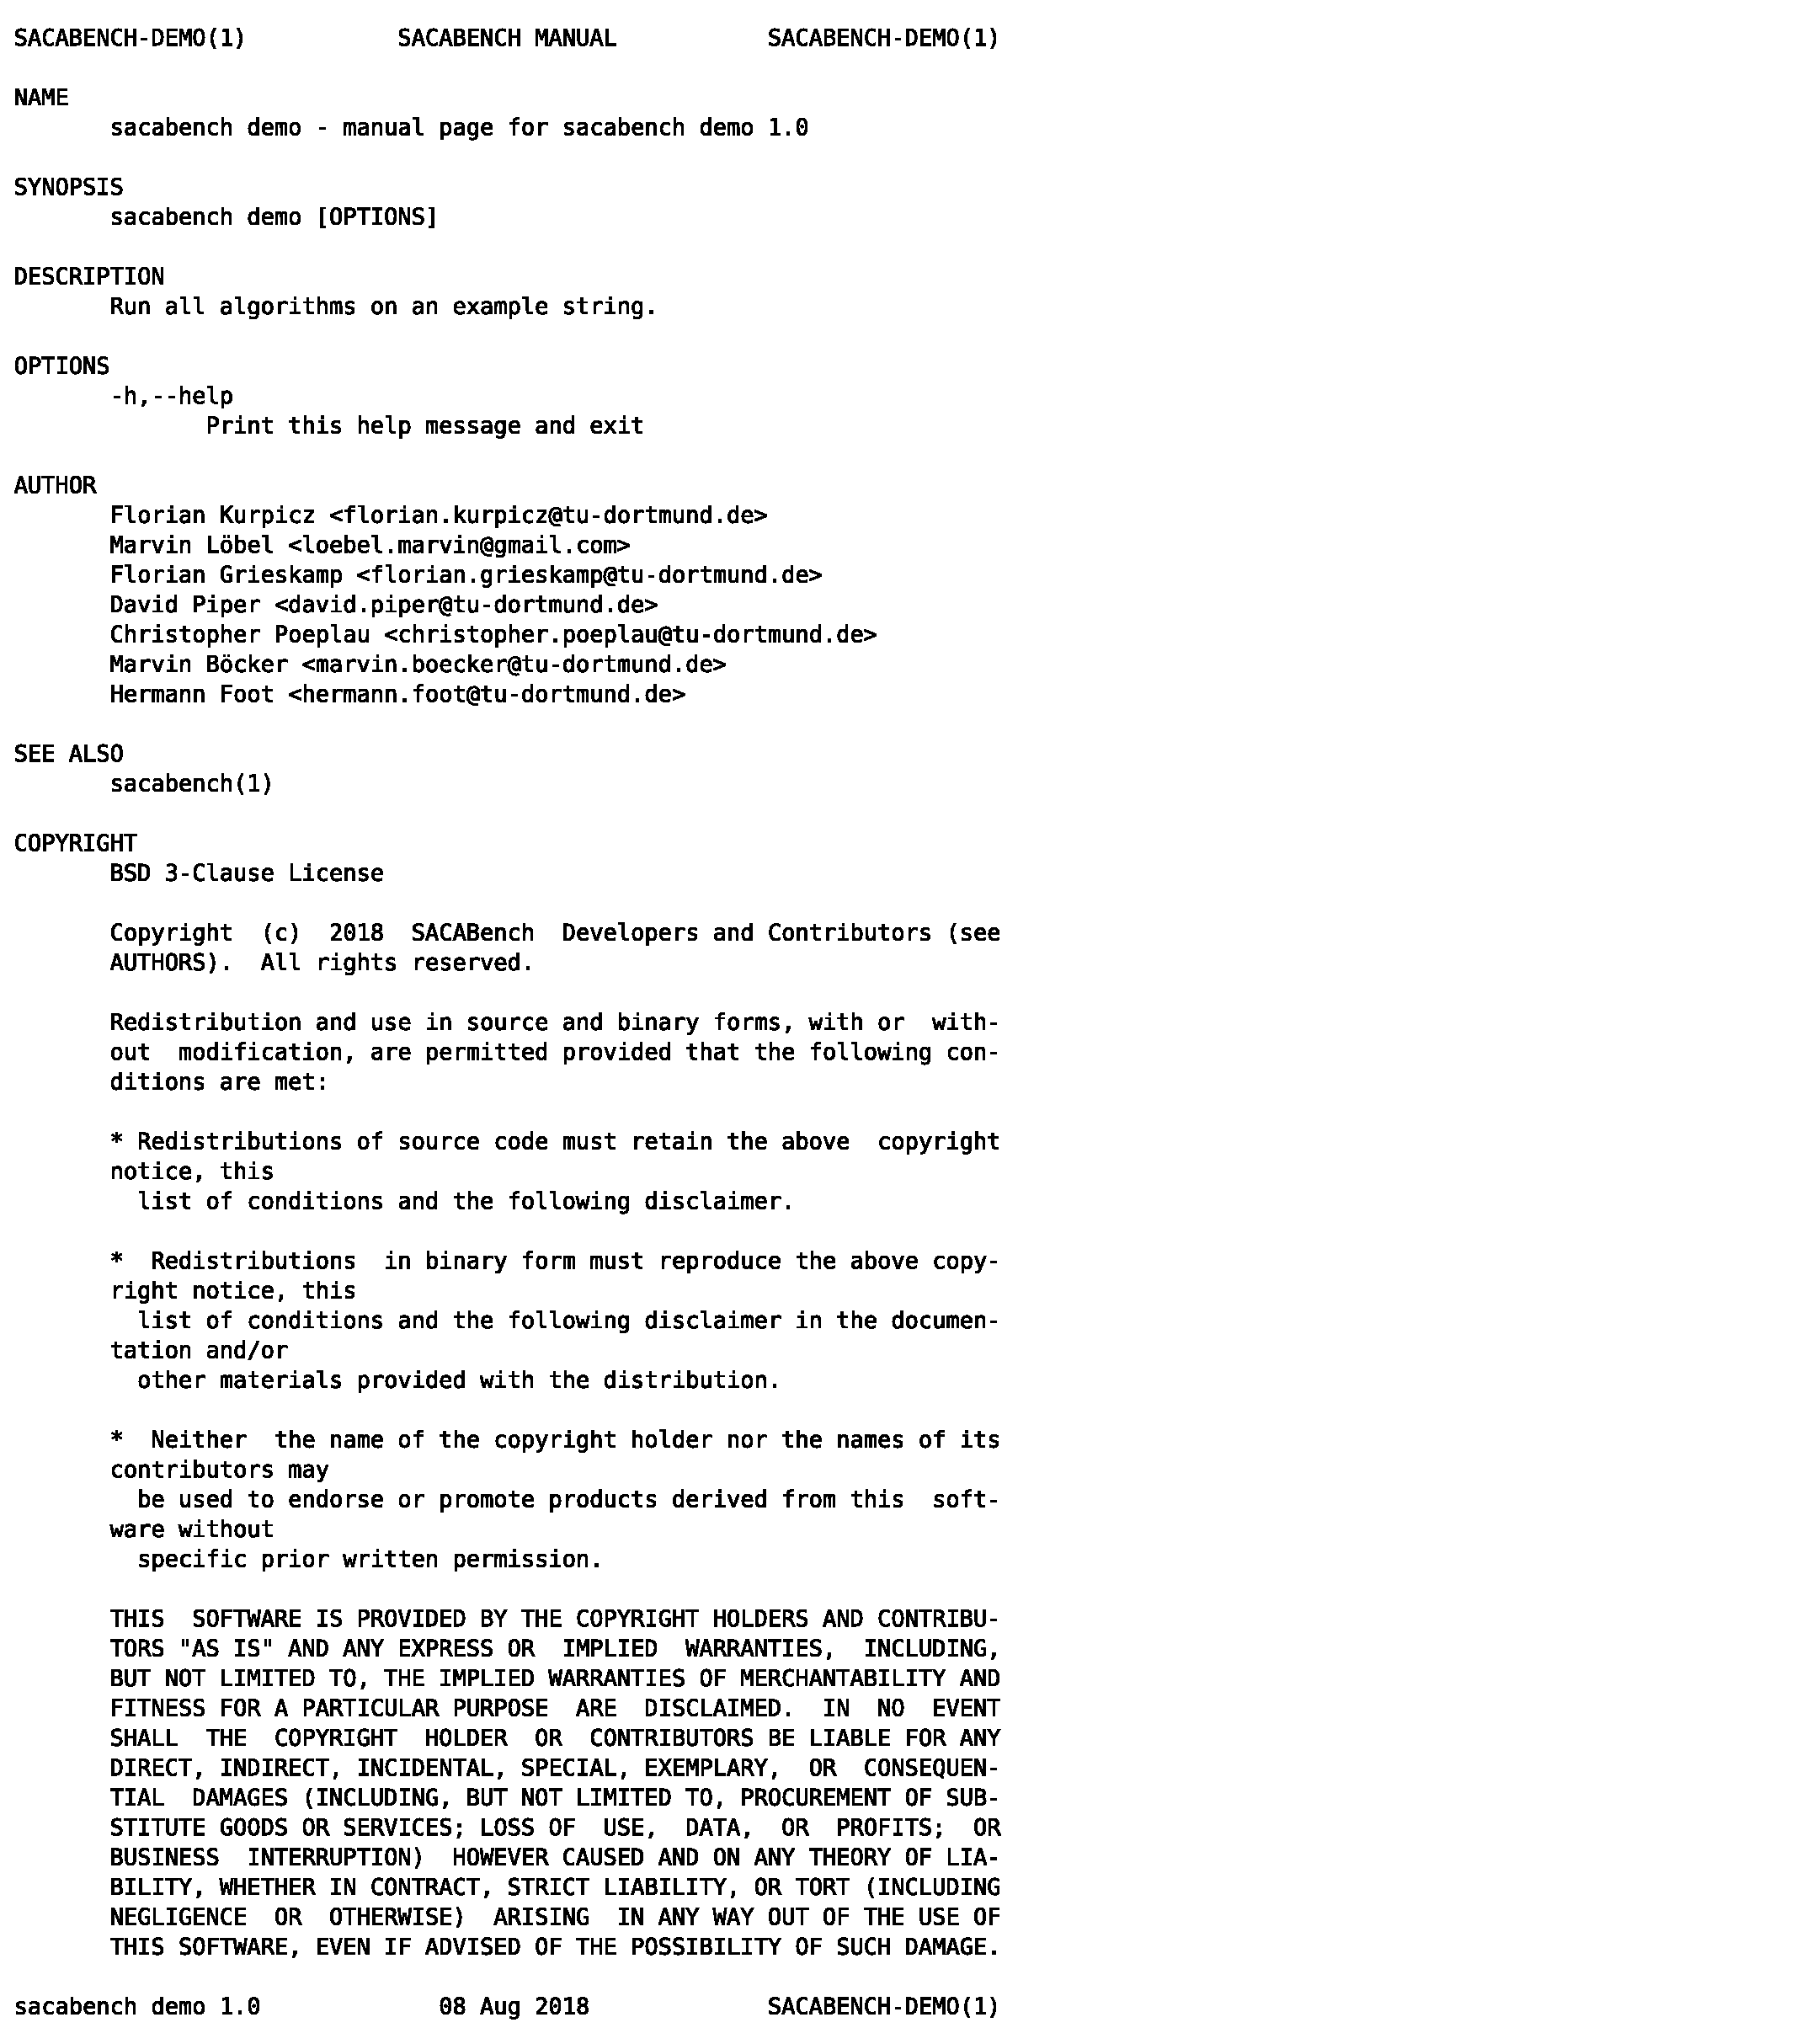
\includegraphics[page=1, viewport=0cm 25cm 20.5cm 26.3cm, clip, width=.5\textwidth]{{kapitel/3_framework/cli/sacabench-demo/sacabench-demo}.pdf}\\
    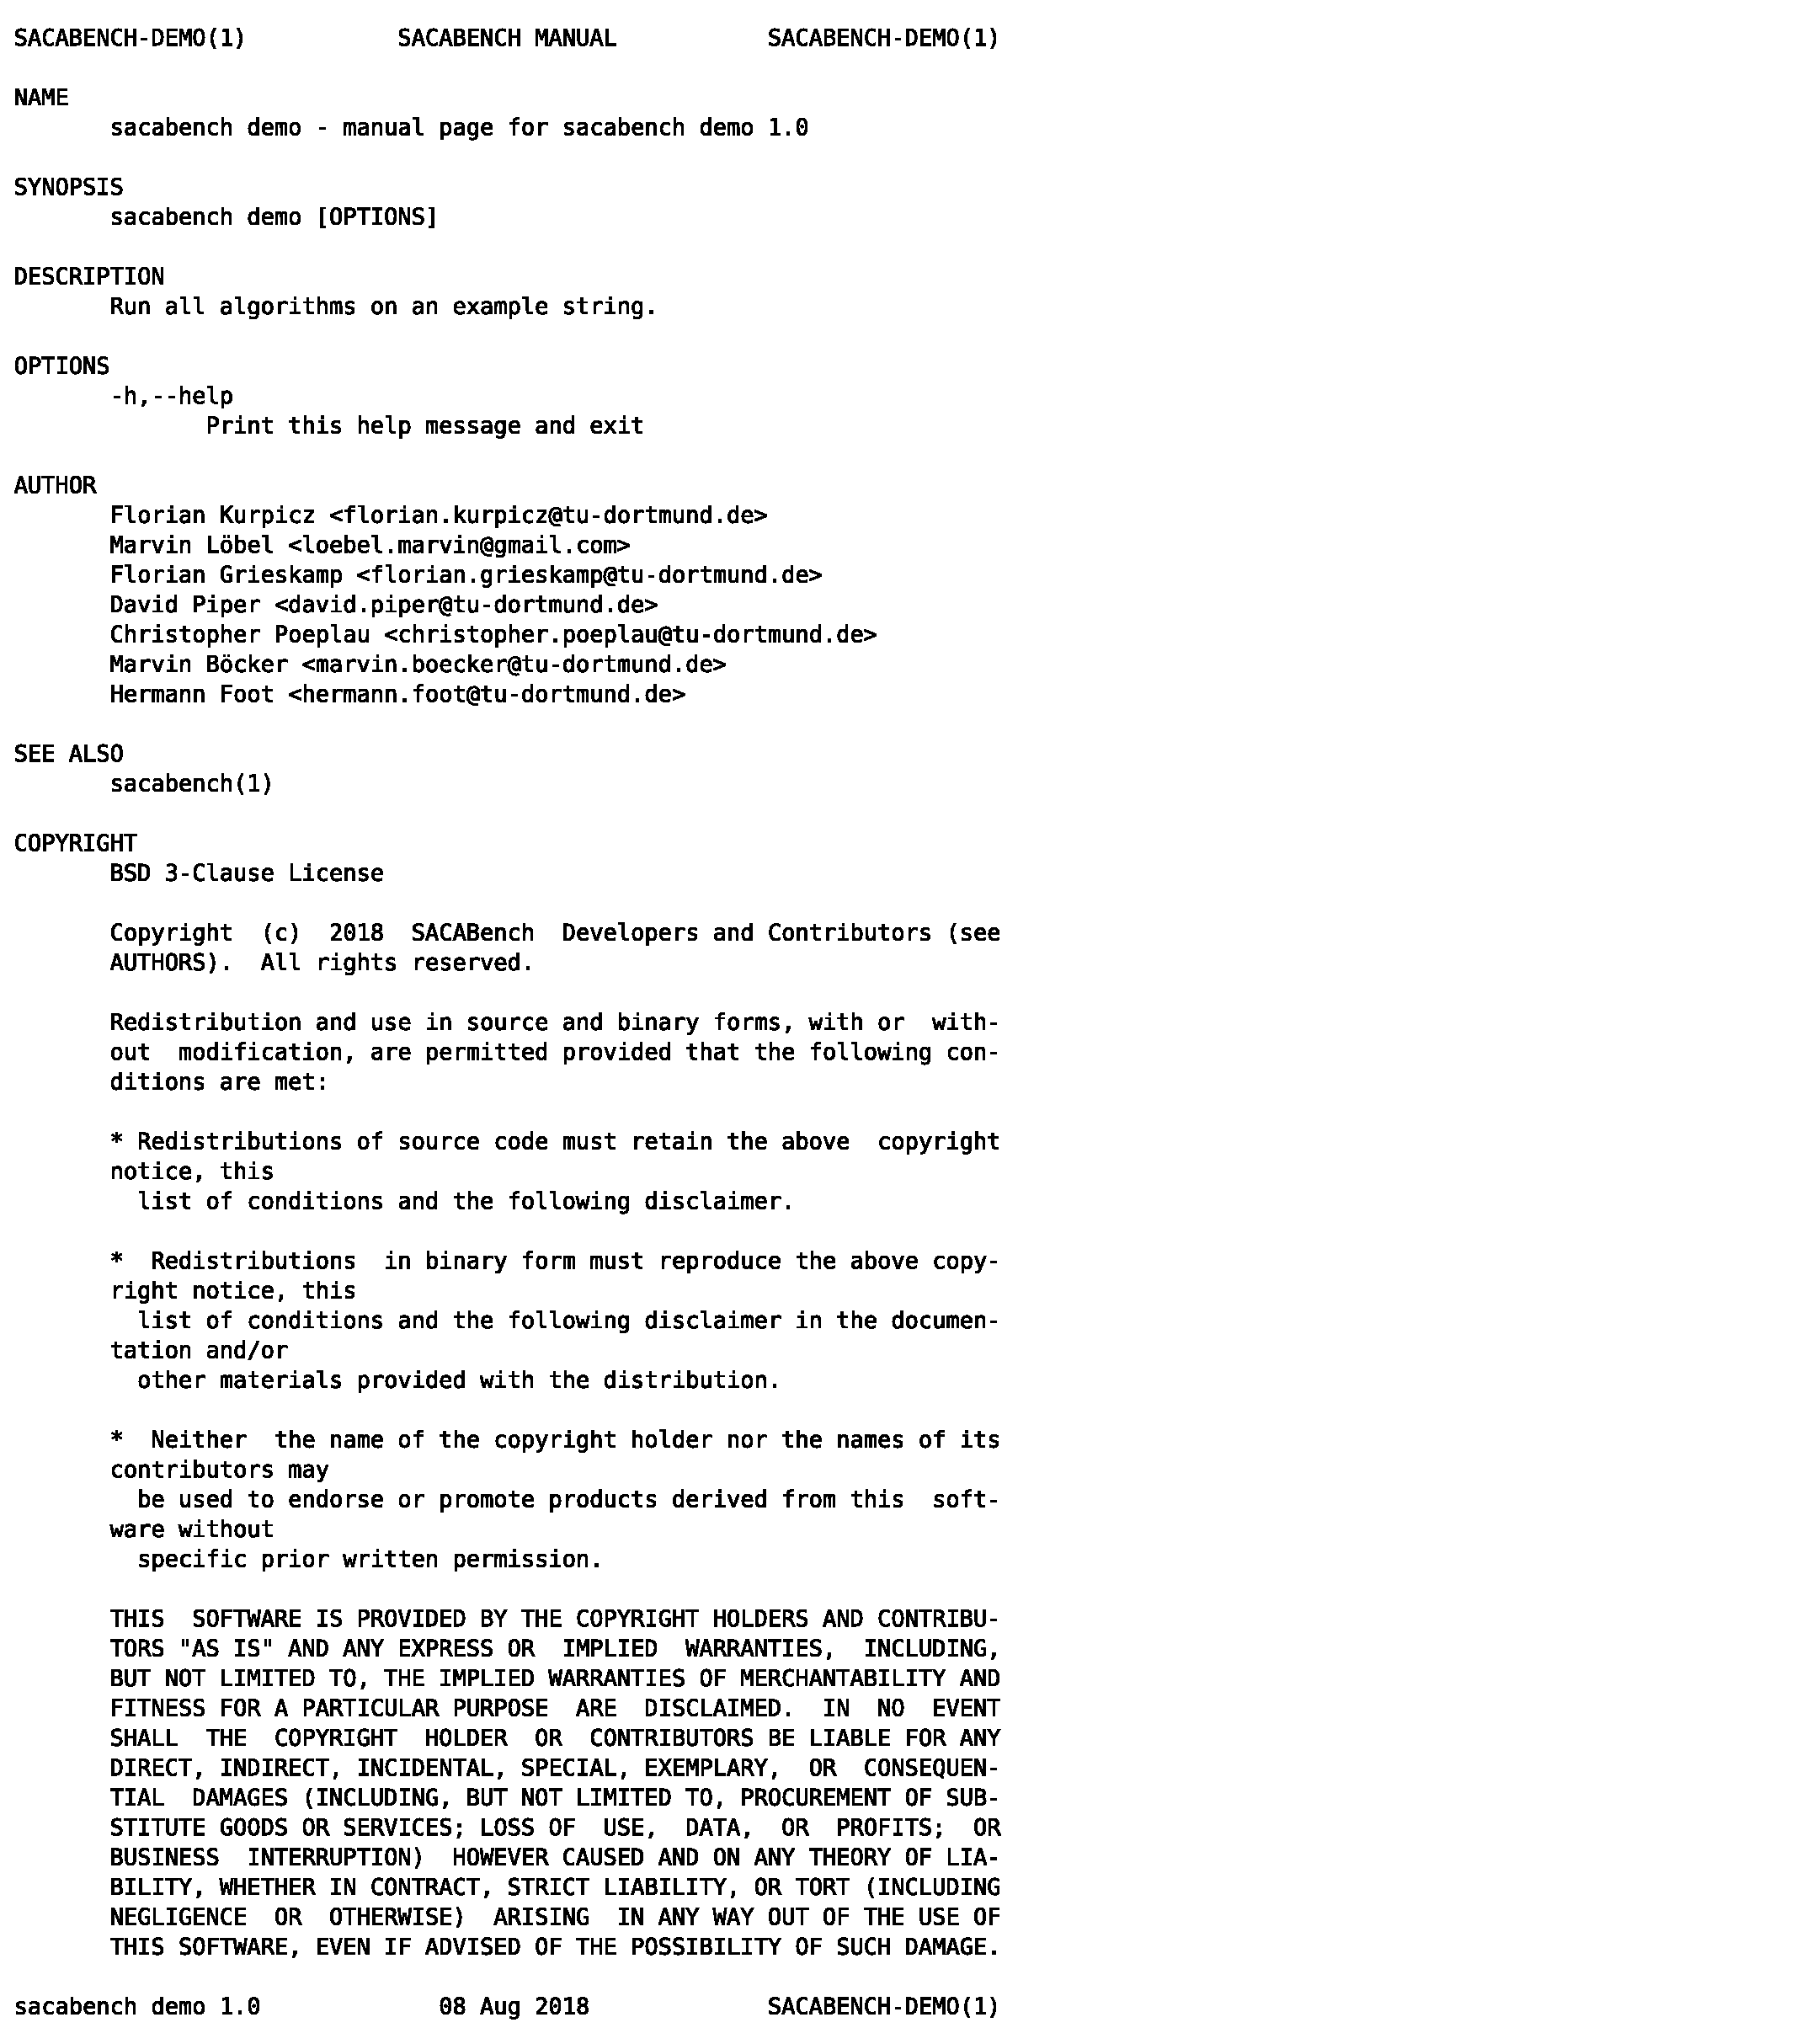
\includegraphics[page=1, viewport=0cm 0cm 20.5cm 1.5cm, clip, width=.5\textwidth]{{kapitel/3_framework/cli/sacabench-demo/sacabench-demo}.pdf}
    \caption{gekürzte Ausgabe von \texttt{man sacabench demo}}
    \label{manpage:sacabench-demo}
\end{wrapfigure}
Mit dem Befehl \texttt{sacabench demo} können alle Algorithmen auf einem kurzen Beispieltext (\glqq \termfont{hello world}\grqq) ausgeführt werden.\par
Diese Funktionalität erfüllt ausschließlich den Zweck, das Framework sowie die Algorithmen auf Lauffähigkeit auf dem verwendeten System zu testen. Auch hier ist eine Hilfeoption über \termfont{-h} bzw. \termfont{-{}-help} erreichbar.\par
}

\subsection{sacabench construct}
\label{framework:cli:sacabench-construct}

{
\begin{wrapfigure}[30]{R}[5mm]{.5\textwidth}
    \vspace{-1.5\baselineskip}
    \includegraphics[page=1, viewport=0cm 32.8cm 20.5cm 68.5cm, clip, width=.5\textwidth]{{kapitel/3_framework/cli/sacabench-construct/sacabench-construct}.pdf}\\
    \includegraphics[page=1, viewport=0cm 25cm 20.5cm 26.3cm, clip, width=.5\textwidth]{{kapitel/3_framework/cli/sacabench-construct/sacabench-construct}.pdf}\\
    \includegraphics[page=1, viewport=0cm 0cm 20.5cm 1.5cm, clip, width=.5\textwidth]{{kapitel/3_framework/cli/sacabench-construct/sacabench-construct}.pdf}
    \caption{gekürzte Ausgabe von \texttt{man sacabench construct}}
    \label{manpage:sacabench-construct}
\end{wrapfigure}

Mit dem Befehl \texttt{sacabench construct} kann ein ausgewählter Algorithmus ausgeführt werden. 
\par
Der auszuf{\"u}hrende Algorithmus wird dabei durch sein K{\"u}rzel bestimmt, wie es bei \termfont{sacabench list} angegeben ist. 
Gefolgt wird der Name des Algorithmus durch den Text, auf den er angewendet werden soll. 
Hierf{\"u}r kann ein Pfad zu einer Textdatei oder alternativ \termfont{-} f{\"u}r STDIN angegeben werden. 
\par
Zus{\"a}tzlich kann eine ganze Reihe von Optionen angegeben werden. 
Wie auch bei anderen Subcommands zeigen \termfont{-h} und \termfont{-{}-help} die Hilfe an. 
Die Option \termfont{-c} bzw. \termfont{-{}-check} wendet zus{\"a}tzlich zu dem ausgew{\"a}hlten Algorithmus einen weiteren SACA auf die Eingabe an und {\"u}berpr{\"u}ft, ob die beiden Ergebnisse gleich sind. 
Ist dies nicht der Fall, wird eine Fehlermeldung angezeigt. 
Eine Alternative hierzu ist die Option \termfont{-q} oder \termfont{-{}-quick}, welche auch die Korrektheit überprüft, jedoch einen parallelen Algorithmus verwendet. 
Wird die Option \termfont{-b} oder \termfont{-{}-benchmark} gefolgt von einem Pfad angegeben, wird an diesem Pfad eine JSON-Datei mit den gemessenen Zeiten und Speicherverbrauch angelegt. 
Existiert an dem angegebenen Pfad bereits eine Datei, kann diese mit der Option \termfont{-f} bzw. \termfont{-{}-force} {\"u}berschrieben und durch die neue Messung ersetzt werden. 
Der Inhalt dieser Datei ist die Grundlage f{\"u}r die durch ein R-Skript erstellten Diagramme, welche mit \termfont{-z} oder \termfont{-{}-rplot} bei der Ausf{\"u}hrung des Algorithmus generiert werden. 
Als Alternative hierzu können durch die Option \termfont{-{}-latexplot} auch Plots durch SqlPlotTools und Latex generiert werden.
Weitere Informationen hierzu sind in Kapitel \ref{framework:bechmark:sqlplottools} enthalten.
Um bei den Messungen ein besseres Ergebnis zu erhalten, kann mit der Option \termfont{-r} bzw. \termfont{-{}-repetitions} eine Anzahl an Durchf{\"u}hrungen festgelegt werden. 
Hierdurch wird die Genauigkeit der Messung erh{\"o}ht, indem das Arithmetische Mittel gebildet wird.
Weiterhin kann dem Befehl \termfont{-p} oder \termfont{-{}-prefix} hinzugef{\"u}gt werden. 
Hierbei kann die Anzahl an f{\"u}hrenden Bytes angegeben werden, die von der Eingabe verarbeitet werden sollen.
Um gr{\"o}{\ss}ere Werte leichter angeben zu k{\"o}nnen, sind die Abk{\"u}rzenden Schreibweisen K und M erlaubt, welche f{\"u}r Kilobyte bzw. Megabyte stehen.
Dies sorgt daf{\"u}r, dass von der {\"u}bergebenen Textdatei nur so viele Bytes verarbeitet werden, wie durch diese Option angegeben werden. 
Die Option \termfont{-B} oder \termfont{-{}-binary} veranlasst das Framework zur Ausgabe in bin{\"a}rer Form.
Anschlie{\ss}end werden die Eintr{\"a}ge des Ergebnisses als Bin{\"a}rzahlen mit bis zu 8 Stellen ausgegeben. 
Die erste Zahl der Ausgabe gibt die genaue Anzahl der Stellen an.
Ist eine feste Anzahl an Bits gew{\"u}nscht, kann diese mit der Option \termfont{-F} bzw. \termfont{-{}-fixed} angegeben werden.
Alternativ kann das Framework das Suffixarray als JSON-Array ausgeben. 
Dies ist mit der Option \termfont{-J} oder \termfont{-{}-json} möglich.
Die nächste Option, welche dem Subcommand \texttt{sacabench construct} {\"u}bergeben werden kann, ist \termfont{-m} oder \termfont{-{}-minimum\_sa\_bits} gefolgt von einem UINT Wert. 
Dieser Parameter bestimmt die Anzahl der Bits, die f{\"u}r die Datenstrukturen w{\"a}hrend der Berechnung genutzt werden.
Anstatt diese Optionen einzeln anzugeben, kann auch eine Konfigurationsdatei eingelesen werden, welche Werte für die zu benutzenden Optionen angibt.
Diese Datei ist im ini-Format und anstelle der Optionen wird die Option \termfont{-{}-config} gefolgt zu dem Pfad zu der Konfigurations-Datei beim Aufruf dieses Befehls angegeben.
Ein Beispiel für solch eine Konfigurations-Datei ist in Abbildung \ref{sacabench-construct:config} zu sehen.
Soll das Tool beispielsweise für den SACA \texttt{BPR} mit der angezeigten Konfigurationsdatei aufgerufen werden, sieht der entsprechende Befehl folgendermaßen aus:

\termfont{sacabench/sacabench construct --config /pfad/zur/config BPR \linebreak /pfad/zum/input/text}

Die gezeigte Konfigurations-Datei ist gleichbedeutentd zum Aufruf mit den Optionen \termfont{-c}, \termfont{-b}, \termfont{-f}, \termfont{-p 1K}, \termfont{-r 2}, \termfont{--rplot} und \termfont{--latexplot}.
Sollen die Optionen einzeln übergeben werden, ist dies mit diesem Aufruf möglich:

\termfont{sacabench/sacabench construct -c -b /ziel/pfad/zur/ergebnis.json -f -p 1K -r 2 --rplot --latexplot BPR /pfad/zum/input/text}
\par
}
\input{kapitel/3_framework/cli/sacabench-construct-config}

\subsection{sacabench batch}
\label{framework:cli:sacabench-batch}

{
    \begin{wrapfigure}[25]{r}[5mm]{.5\textwidth}
    \vspace{-1.5\baselineskip}
    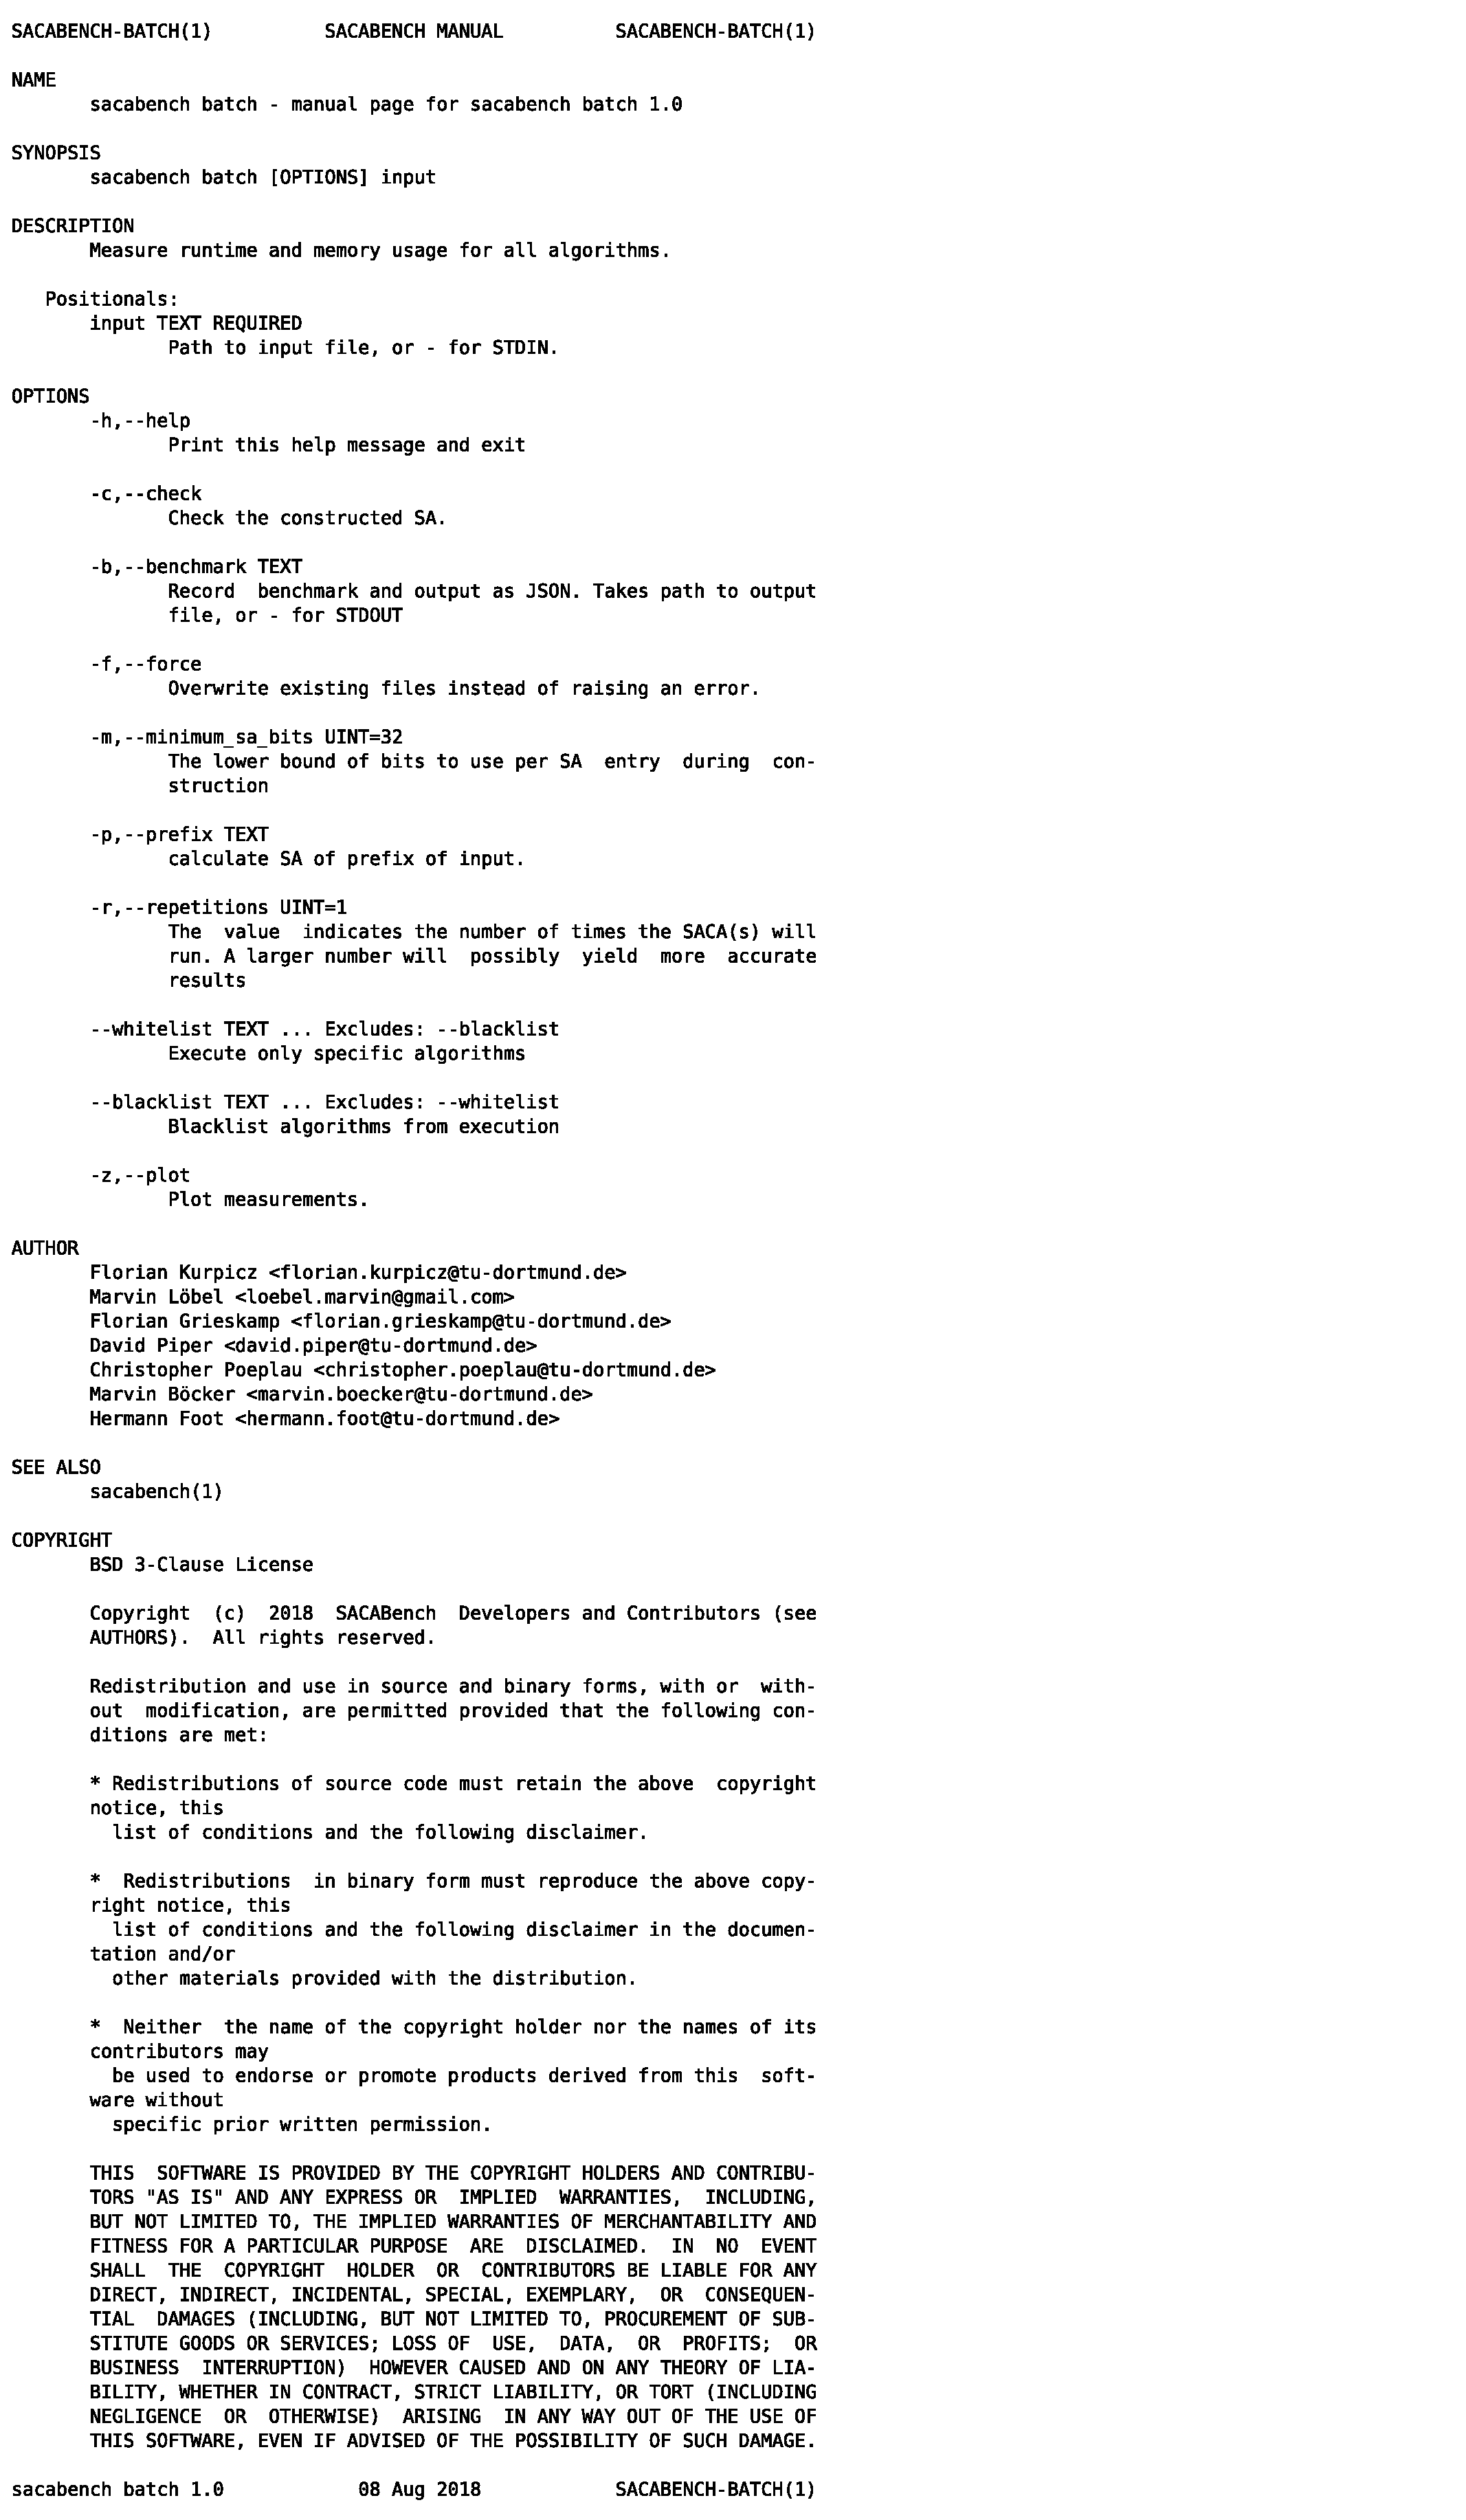
\includegraphics[page=1, viewport=0cm 32.8cm 20.5cm 62.0cm, clip, width=.5\textwidth]{{kapitel/3_framework/cli/sacabench-batch/sacabench-batch}.pdf}\\
    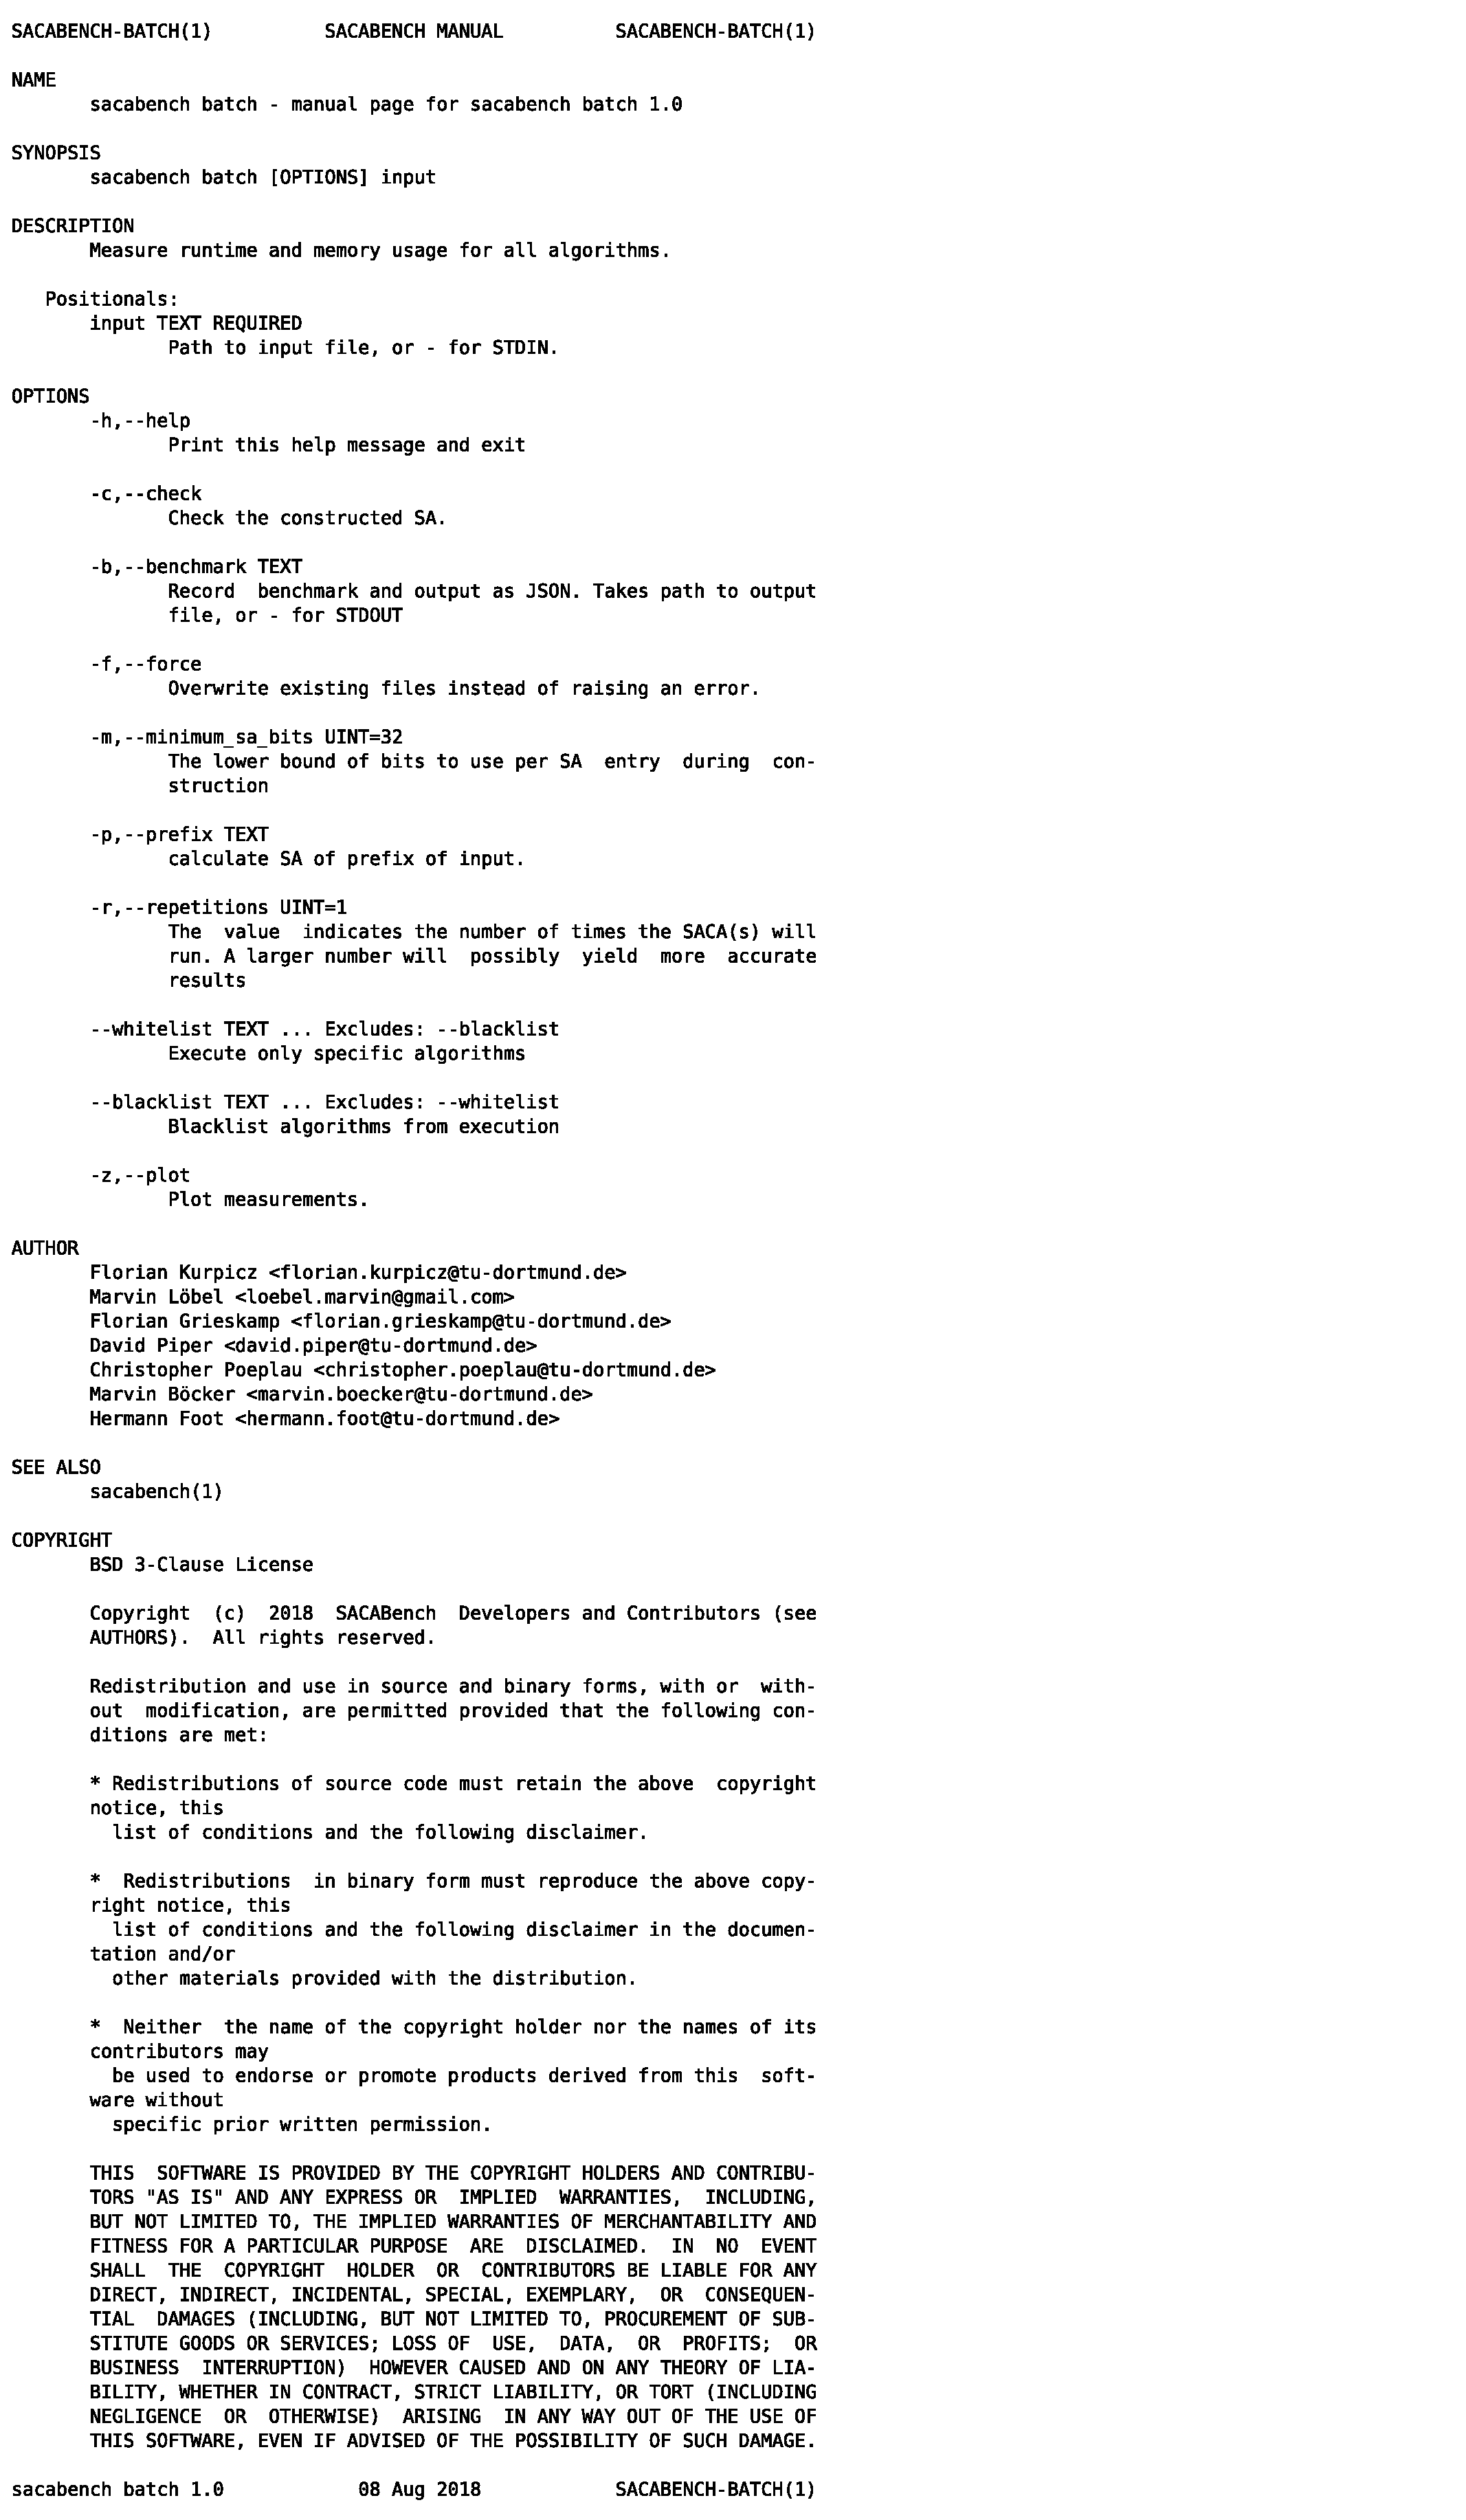
\includegraphics[page=1, viewport=0cm 25cm 20.5cm 26.3cm, clip, width=.5\textwidth]{{kapitel/3_framework/cli/sacabench-batch/sacabench-batch}.pdf}\\
    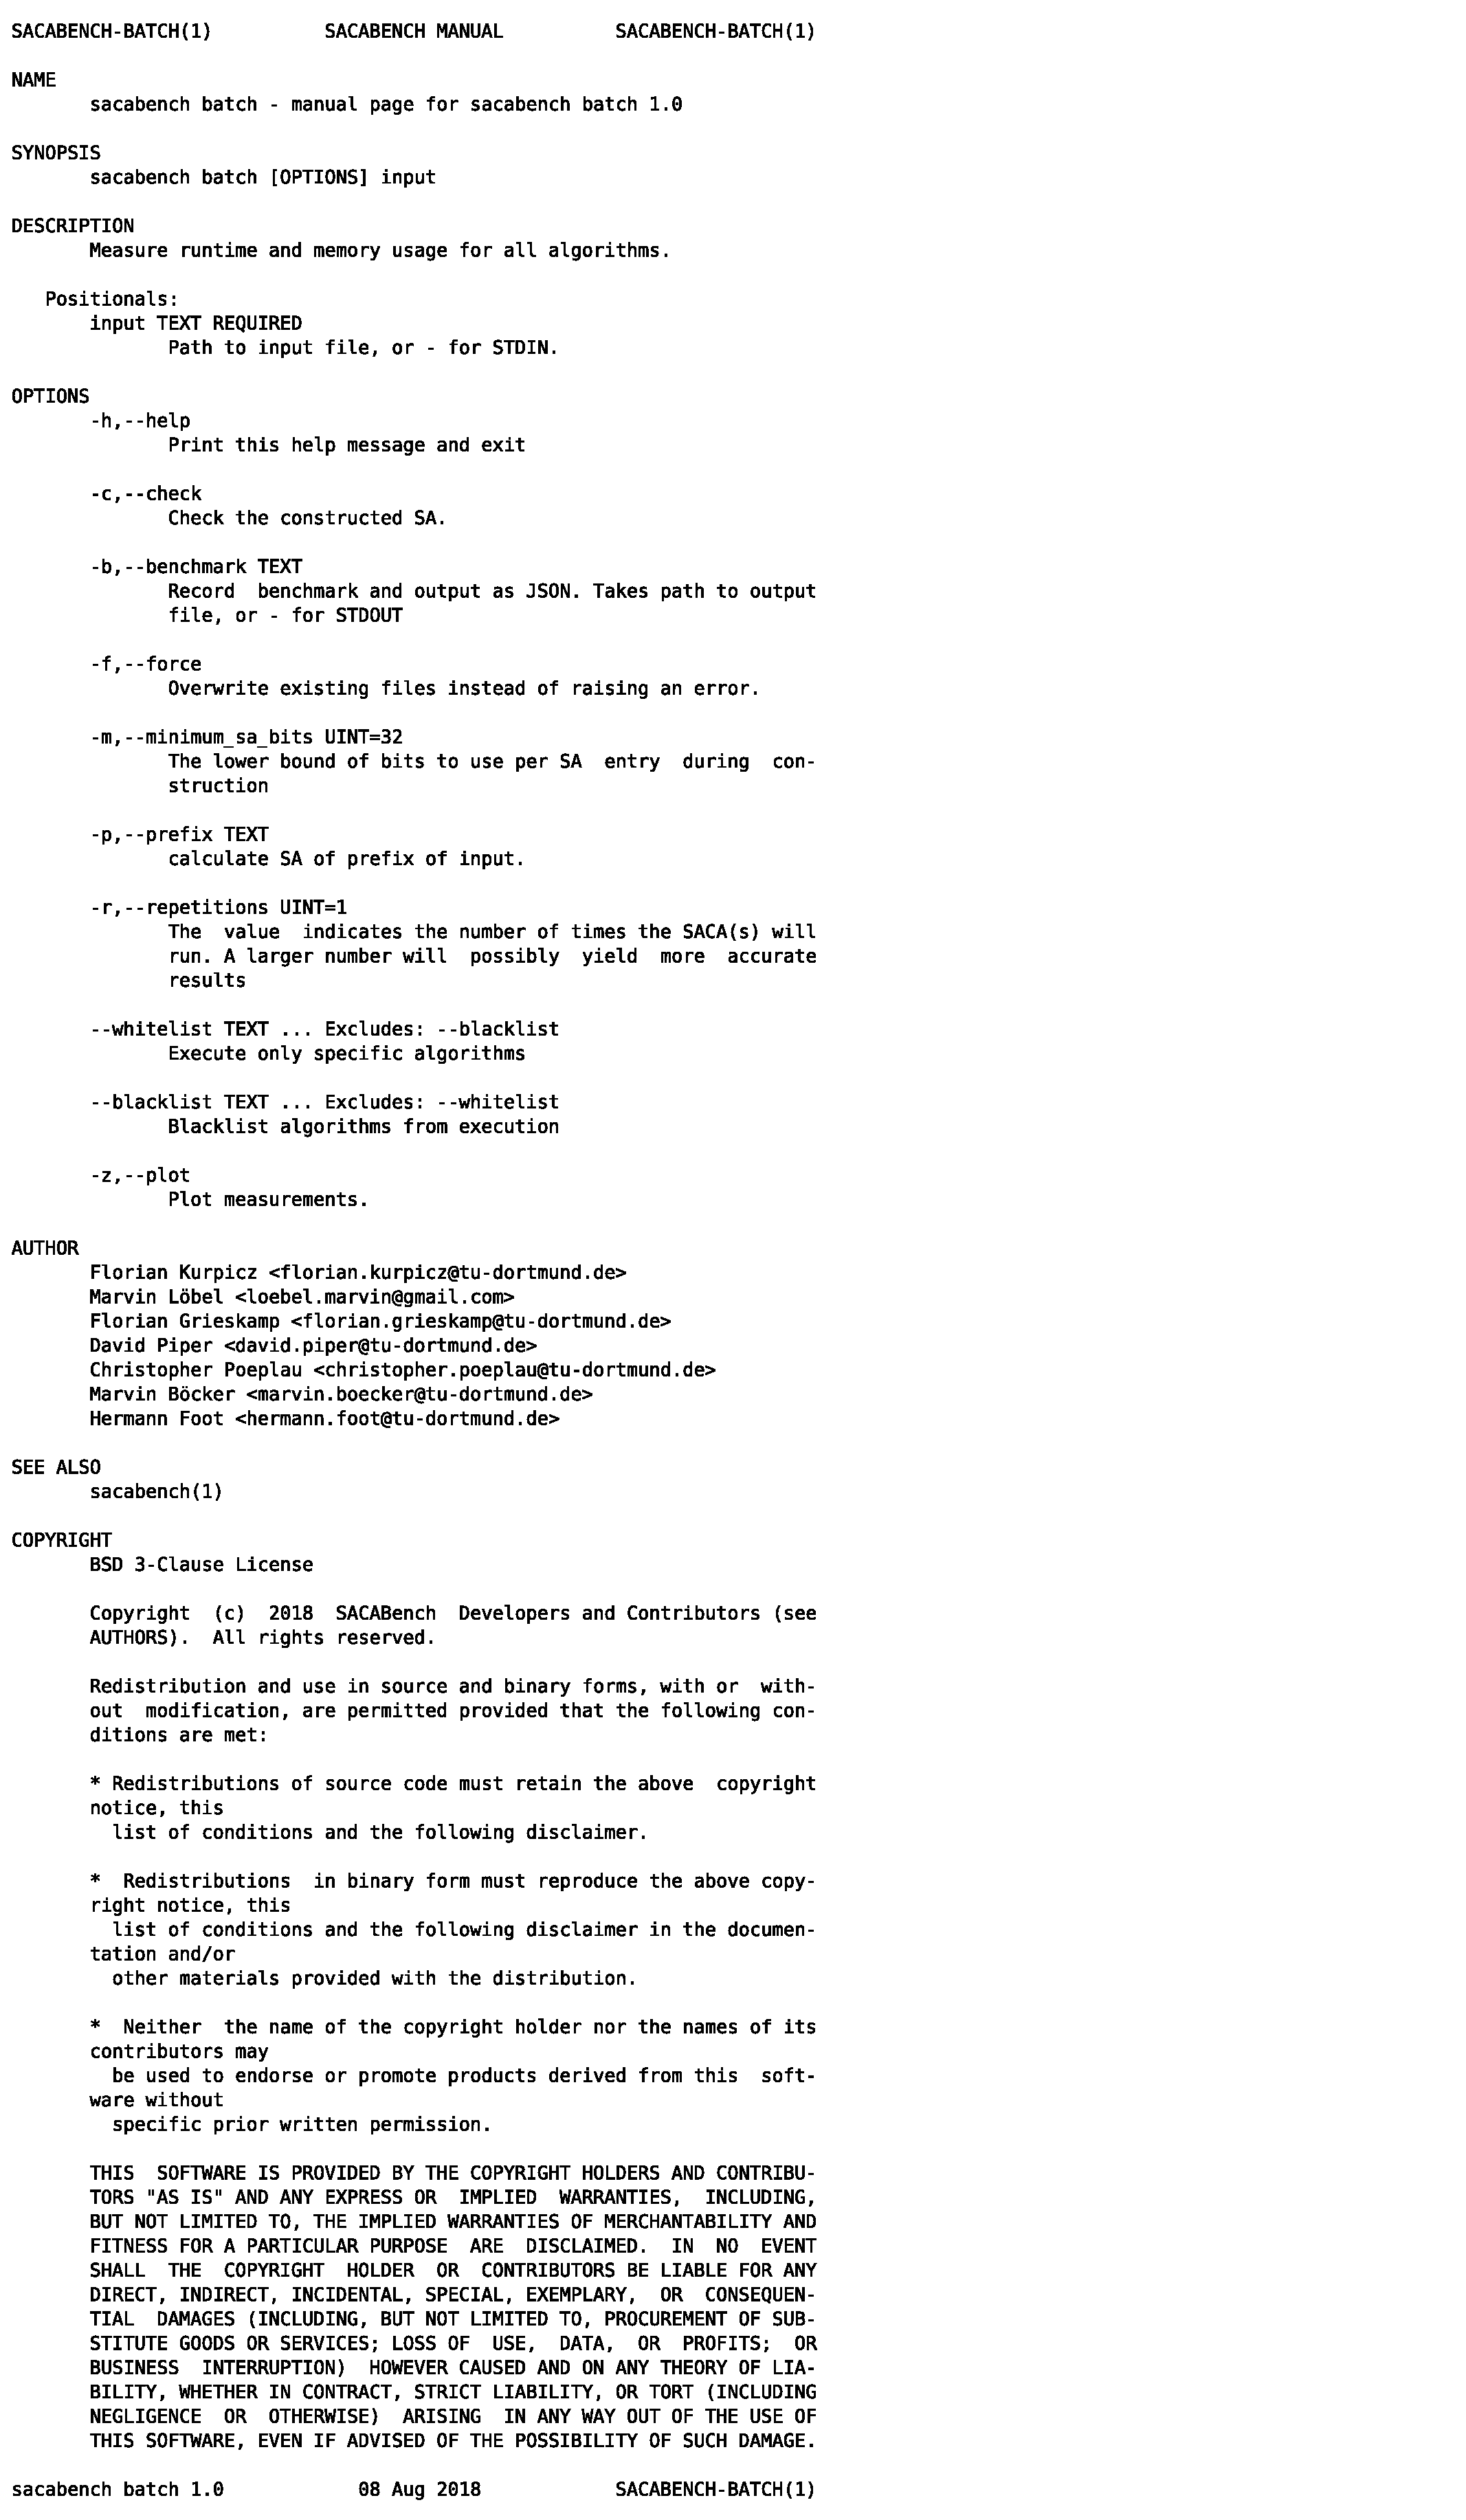
\includegraphics[page=1, viewport=0cm 0cm 20.5cm 1.5cm, clip, width=.5\textwidth]{{kapitel/3_framework/cli/sacabench-batch/sacabench-batch}.pdf}
    \caption{gekürzte Ausgabe von \texttt{man sacabench batch}}
    \label{manpage:sacabench-batch}
\end{wrapfigure}

Mit dem Befehl \texttt{sacabench batch} können mehrere Algorithmen auf der gleichen Eingabedatei ausgeführt werden. Die Funktionalität setzt hautpsächlich auf dem Interface von \termfont{sacabench construct} auf, weshalb ein Großteil der dort verwendbaren Optionen auch hier Anwendung findet. Zu Beachten ist jedoch, dass die Ausgaben aller Algorithmen nach der Ausführung und einem optionalen Test auf Korrektheit verworfen werden. Alle das Ausgabeformat betreffenden Optionen von \termfont{sacabench construct} sind daher für \termfont{sacabench batch} ungültig.\par
Um nicht für jede Messung alle Algorithmen ausführen zu müssen, besteht die Option, wahlweise mit \termfont{-{}-blacklist} einzelne Algorithmen von der Ausführung auszuschließen oder mit \termfont{-{}-white\-list} nur explizit angegebene Algorithmen zu berechnen. Für beide Optionen entsprechen die Namen der anzugebenden Algorithmen denen aus \termfont{sacabench list} (\cref{framework:cli:sacabench-list}).
Benchmarks können wie genau wie zuvor mit \termfont{-{}-benchmark} unter Angabe eines Dateinamens angelegt werden. Die mit \termfont{-{}-plot} generierten Diagramme unterscheiden sich jedoch von den mit \termfont{sacabench construct} erstellten Diagrammen: Der Schwerpunkt liegt hier auf der Vergleichbarkeit der Algorithmen, weshalb in den Diagrammen gezielt die Laufzeit- und Speichermessungen aller ausgeführten Algorithmen miteinander verglichen werden. Eine ausführlichere Beschreibung der Diagramme sowie der zur Aufzeichnung der Benchmakrs verwendeten Techniken ist in \cref{framework:benchmarks} zu finden.\par
}

\subsection{sacabench plot}
\label{framework:cli:sacabench-plot}

Der Befehl \texttt{sacabench plot} erstellt nachträglich zu einer Messung die PDF-Dateien. 
Wurde beispielsweise vergessen, bei \texttt{sacabench construct} oder \texttt{saca\-bench batch} die Option zum Plotten anzugeben, können so die erhaltenen Messdaten dennoch ausgewerted werden.
Hierzu werden dem Befehl die verwendete Messmethode, der Pfad zur Textdatei, die verarbeitet wurde, und der Pfad zur JSON-Datei mit den Ergebnissen übergeben.


\section{Benchmark System}
\label{framework:benchmarks}

Ein \currentauthor{Johannes Bahne} Ziel der Projektgruppe \sacabench ist der Vergleich aller selbst implementierten Algorithmen und importierten Referenz-Implementierungen. Für die bessere Übersicht und Darstellung werden verschiedene Diagramme verwendet, die in diesem Kapitel näher beschrieben werden.

\subsection{Voraussetzungen}

\begin{description}
	\item[\termfont{R - Version}] Die Ergebnisse des Benchmark Systems werden mit Hilfe der Programmiersprache \texttt{R} ausgewertet. \texttt{R} ist eine \emph{Open-Source-Software} für statistische Berechnungen und Grafiken. Daher muss auf dem auszuführenden Computer ein \texttt{R}-Compiler installiert sein\cite{r-project}. Das \texttt{R}-Skript verwendet unter anderem das Paket \termfont{rjson}, welches erst ab der Version \texttt{R} $\geq 3.1.0$ unterstützt wird\cite{rjson}. Aus diesem Grund wird die Version \texttt{R} $\geq 3.1.0$ vorausgesetzt.
	\item[\termfont{Administrationsrechte}] Das \texttt{R}-Skript benötigt neben dem Paket \termfont{rjson} auch das Paket \termfont{RColorBrewer} \cite{rcolorbrewer}. Beide Pakete werden automatisch installiert, wenn sie nicht vorher schon manuell installiert worden sind. Für diese Installation werden jedoch gegebenenfalls Administrationsrechte benötigt. Außerdem sind zum Beispiel für Computer mit Betriebssystem \texttt{macOS} Schreib- und Leserechte bestimmter Verzeichnisse notwendig. Daher wird empfohlen, die Befehle als Administrator auszuführen, indem zum Beispiel das Schlüsselwort \termfont{sudo} verwendet wird.
\end{description}

\subsection{JSON}

Wird die Option \termfont{-b} oder \termfont{-{}-benchmark} für den Befehl \texttt{sacabench construct} und \texttt{sacabench batch} des \sacabench-Frameworks angefügt, wird eine \texttt{JSON}-Datei erzeugt. \texttt{JSON} - Abkürzung für \texttt{JavaScript Object Notation} - ist ein Datenformat, das im Rahmen des \sacabench-Frameworks als Speicherformat aller benötigten Bench\-mark-Werte verwendet wird. In dieser Datei werden unter anderem der Name, die Anzahl der benötigten zuzüglichen Sentinels, der maximale Speicherverbrauch und die Laufzeit des Algorithmus, die Größe des zu untersuchenden Ausgangstextes, die Größe des Datentyps für das Ausgabe-Suffix-Array und die Titel jeder einzelnen Phase des Algorithmus gespeichert. Diese Datei wird anschließend mit einem \texttt{R}-Skript ausgewertet, indem die Option \termfont{-z} oder \termfont{-{}-plot} an die jeweiligen Befehle in der Kommandozeile angehangen werden.


\subsection{Untersuchung einzelner Algorithmen}
\label{framework:bechmark:sacabench-construct}

\begin{wrapfigure}{R}{.5\textwidth}
	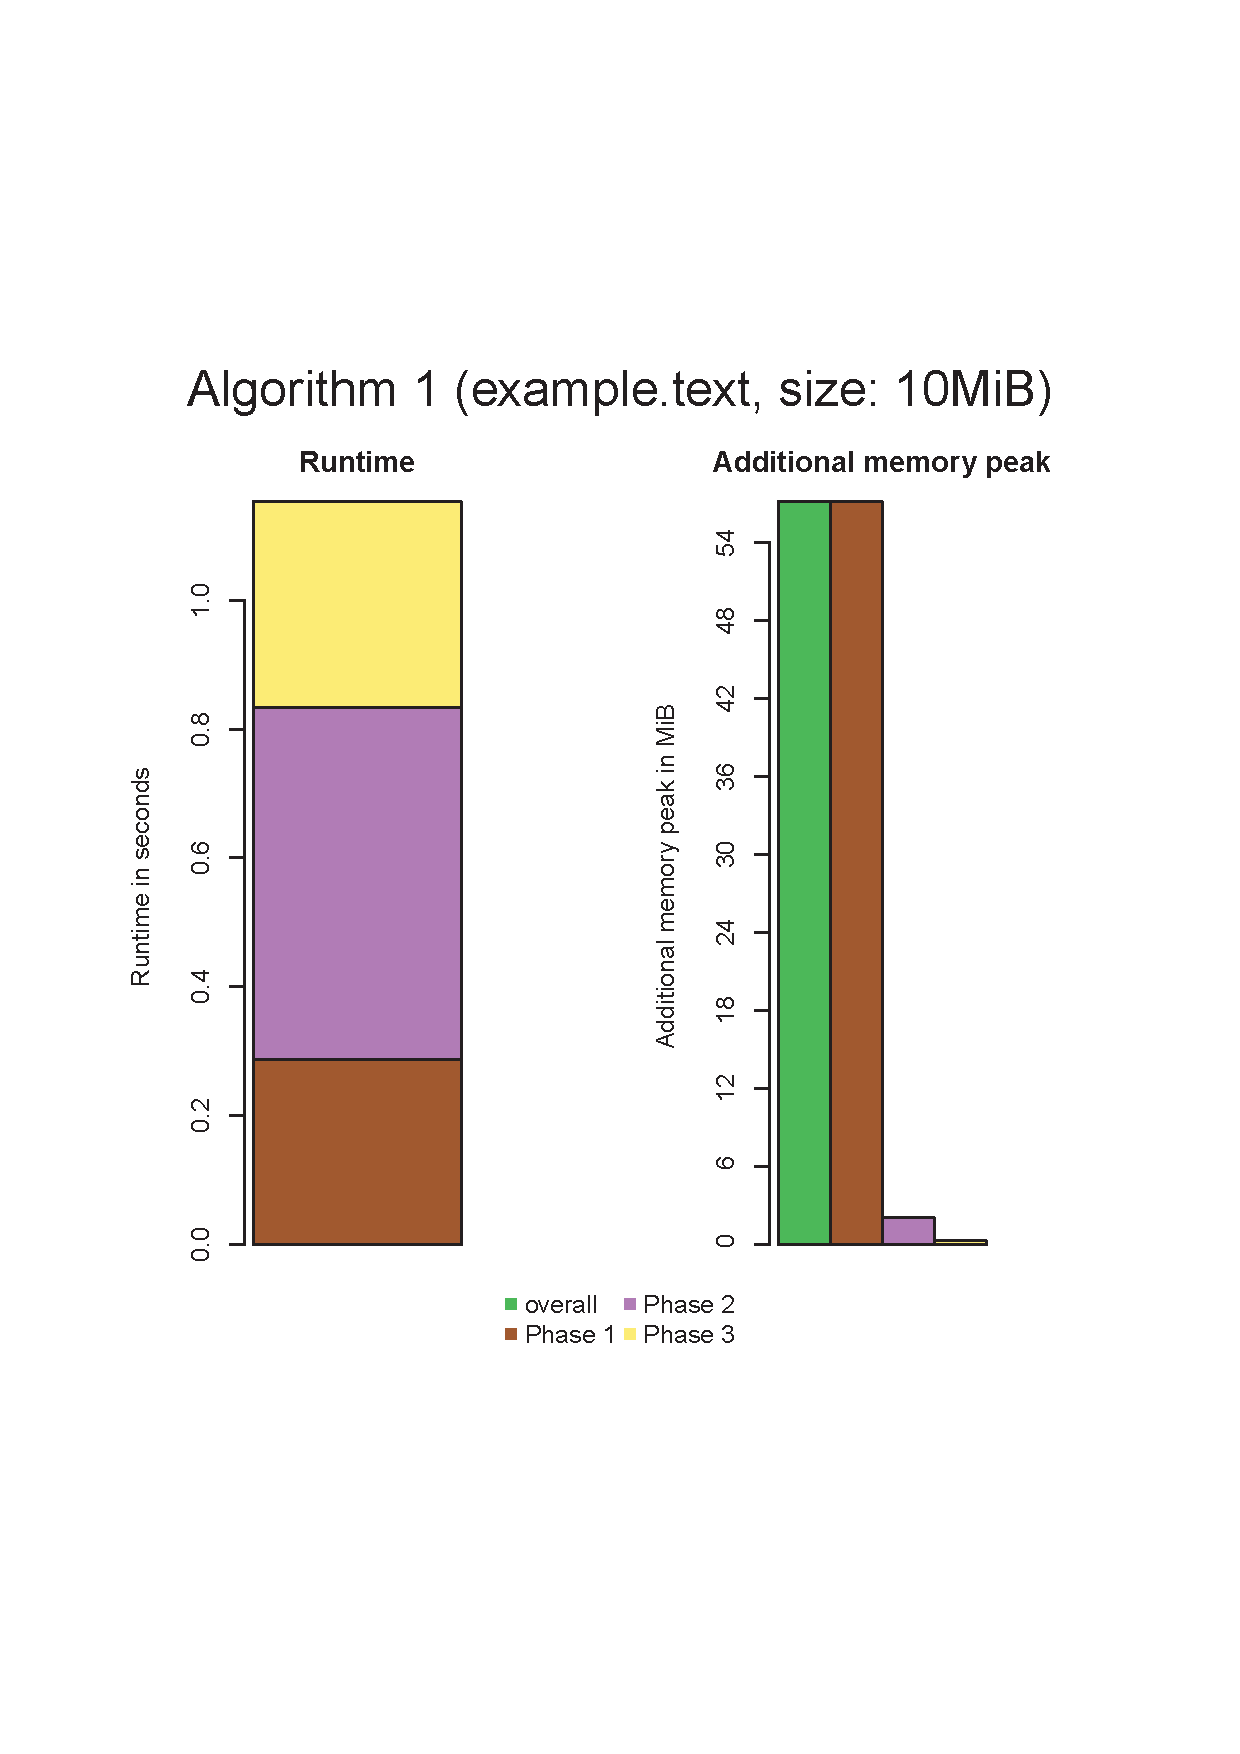
\includegraphics[page = 1, width=.5\textwidth]{kapitel/3_framework/benchmark/sacabench-construct/beispiel_construct.pdf}
	\caption{Messergebniss eines Beispiel-Algorithmus}
	\label{pdf:benchmark:construct}
\end{wrapfigure}


Wird die \texttt{plot}-Option mit dem Befehl \texttt{sacabench construct} ausgeführt, lassen sich einzelne Algorithmen näher untersuchen. Dabei wird die Laufzeit und der maximale Speicherverbrauch des Algorithmus während der Erstellung des Suffix-Arrays gemessen. Zusätzlich gibt es die Möglichkeit, Implementierungen der Algorithmen in Phasen aufzuteilen. Dies ermöglicht eine bessere Übersicht und gegebenenfalls eine schnellere Auffindung von Schwachstellen der eigenen Implementierungen.
Als Ergebnis wird eine zweiseitige \texttt{PDF}-Datei erstellt, die in dem Pfad abgespeichert wird, der hinter der Option \termfont{-b} oder \termfont{-{}-benchmark} angegeben worden ist.

Die \cref{pdf:benchmark:construct} zeigt die erste Seite der \texttt{PDF}-Datei. Dort ist als Überschrift sowohl der Name des Algorithmus als auch der zu untersuchende Text mit dessen Größe angegeben. Die darunter abgebildete Grafik stellt die Messergebnisse dar. Die Grafik ist wiederum in zwei Bereiche aufgeteilt. Auf der linken Seite ist ein gestapeltes Säulendiagramm zu erkennen, das die Laufzeit repräsentiert. Jeder Stapel auf diesem Säulendiagramm entspricht der Laufzeit einer Phase. Die Zeiteinheit, die auf der Y-Achsenbeschriftung niedergeschrieben ist, wird dabei je nach Laufzeit angepasst, sodass die Übersicht gewahrt ist. Auf der rechten Seite befindet sich ein Säulendiagramm, das den Speicherverbrauch widerspiegelt. Auch hierbei stellt jede Säule eine Phase dar. Der Speicherverbrauch wird so gemessen, dass pro Phase jeweils der maximal gemessene Verbrauch des Speichers ohne Berücksichtigung des Ausgangstextes dargestellt ist. Welche Phase zu welchem Stapel, beziehungsweise welcher Säule gehört, ist der Le\-gen\-de, die sich in der Fußzeile der ersten Seite befindet, zu entnehmen.

Auf der zweiten Seite befindet sich eine Auflistung der tech\-nisch\-en Daten des auszuführenden Systems, das sogenannte \texttt{experimental setup}. Dazu gehört der Prozessor mit der zugehörigen Frequenz, sowie die maximale Turbo-Frequenz. Ebenfalls wird die Größe des Ar\-beits\-spei\-chers angezeigt. Zusätzlich wird auch auf dieser Seite erneut der Name und die Größe des Textes angegeben, zu dem das Suffix-Array erstellt worden ist.
\subsection{Vergleich mehrerer Algorithmen}
\label{framework:bechmark:sacabench-batch}

\begin{wrapfigure}{R}{.5\textwidth}
	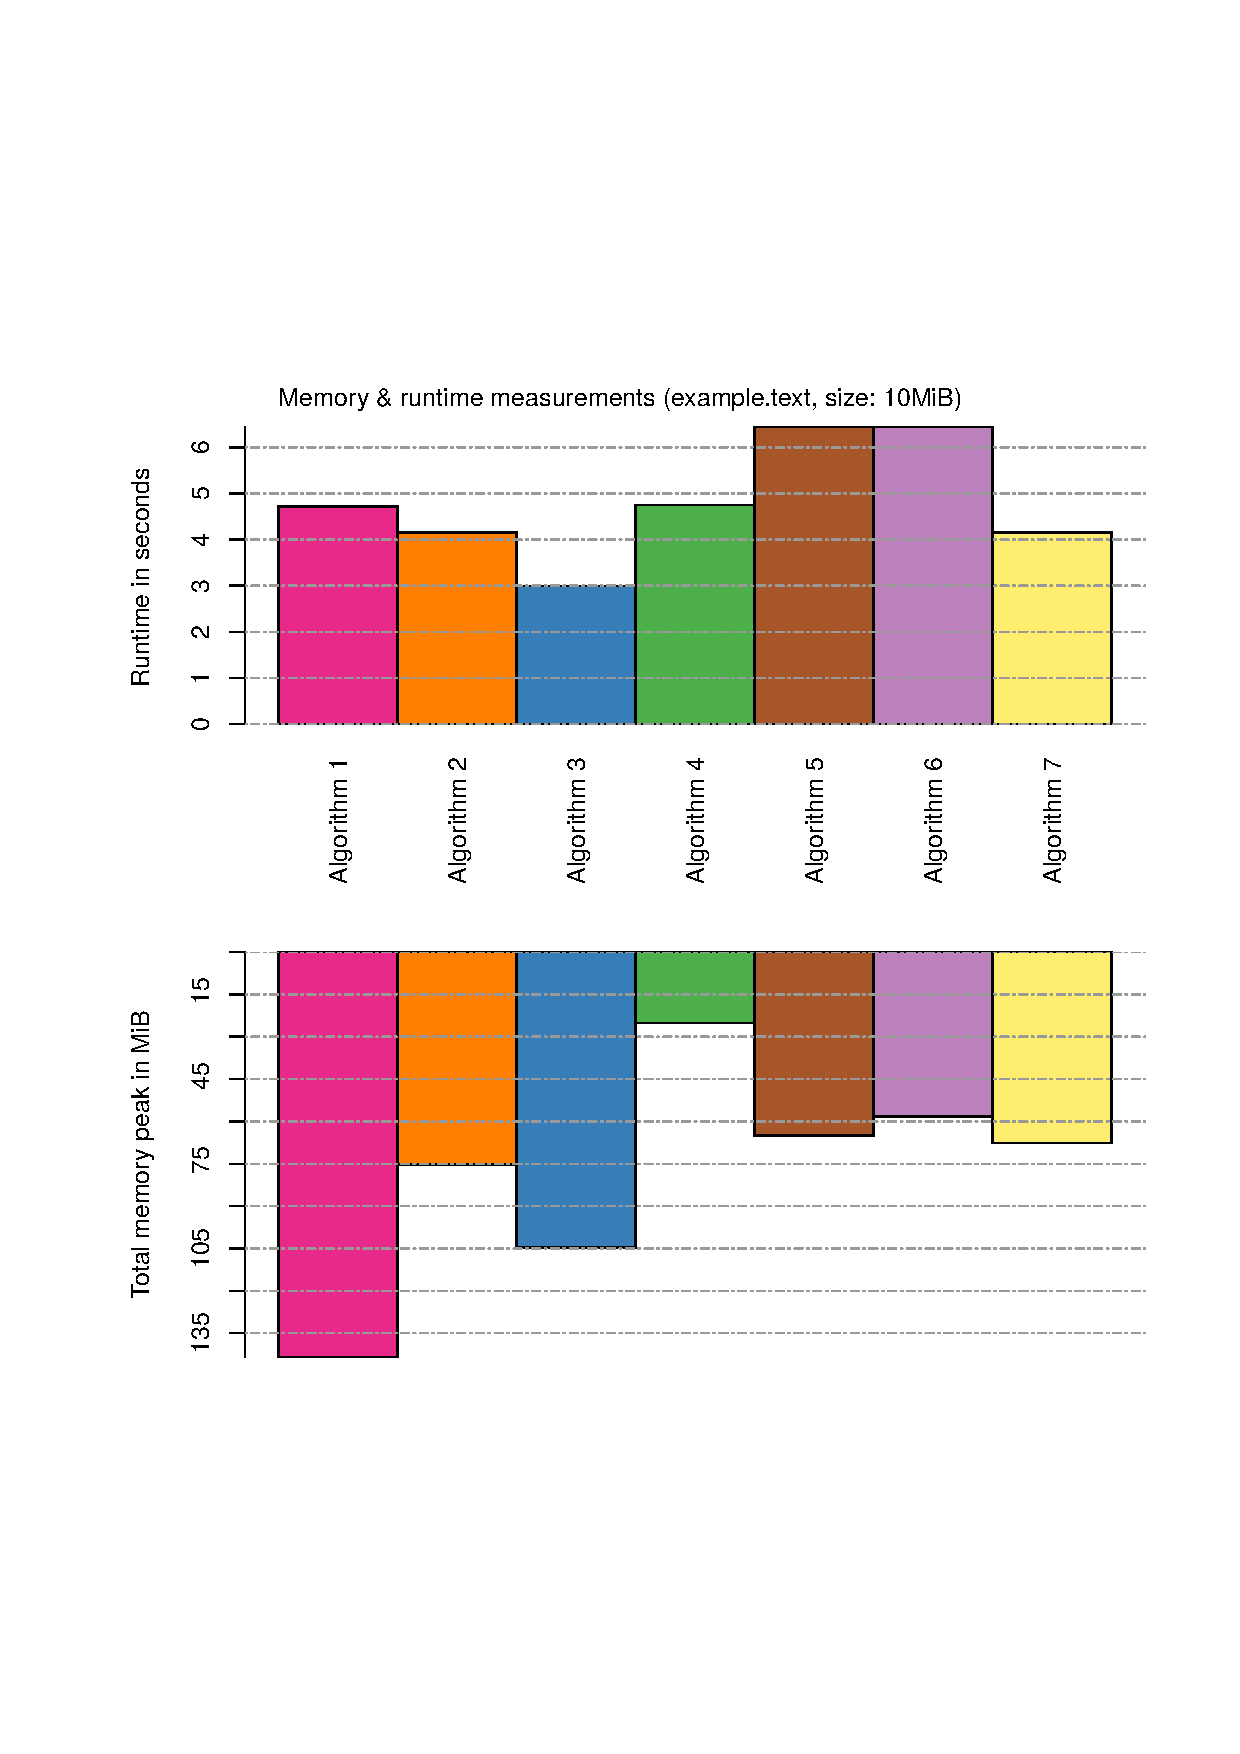
\includegraphics[page = 1, width=.5\textwidth]{kapitel/3_framework/benchmark/sacabench-batch/beispiel_batch_saeule.pdf}
	\caption{Messergebnisse mehrerer Algorithmen}
	\label{pdf:benchmark:batch:saeule}
\end{wrapfigure}

Ist jedoch nach den Messergebnissen aller vorhandenen Algorithmen in dem \sacabench-Framework gefragt, wird der Befehl \texttt{sacabench batch} mit der Option \termfont{-z} oder \termfont{-{}-plot} verwendet. Dabei wird von jedem Algorithmus die Laufzeit und der Spei\-cher\-ver\-brauch gemessen. Diese Messungen schaffen einen Überblick aller Algorithmen. Anders als bei den Ergebnissen einzelner Algorithmen, wird hierbei der Übersicht halber auf die Unterteilung in Phasen verzichtet. Die dabei erstellte \texttt{PDF}-Datei enthält sieben Seiten.

Die \cref{pdf:benchmark:batch:saeule} zeigt die erste Seite der \texttt{PDF}-Datei. Auf dieser sind zwei Säulendiagramme abgebildet. Das obere Diagramm repräsentiert die jeweiligen Laufzeiten und das untere Diagramm zeigt den maximalen Spei\-cher\-ver\-brauch inklusive des Ausgangstextes - beides jeweils in passenden Einheiten. Jede einzelne Säule eines Diagramms steht für einen Algorithmus. In der Mitte beider Diagramme sind die dazugehörigen Namen der Algorithmen wiederzufinden. Auf der ersten Seite sind diese Algorithmen aufsteigend nach Namen sortiert. Diese Reihenfolge ermöglicht einen besseren Vergleich der Messergebnisse unserer Implementierungen mit den Ergebnissen der Referenzimplementierungen, da diese bis auf das Suffix \texttt{\_ref} den gleichen Namen haben und somit nebeneinander aufgelistet werden.

Auf der zweiten Seite sind die selben Messungen wiederzufinden, jedoch ist das Säulendiagramm aufsteigend nach der Laufzeit umsortiert worden. Dadurch lässt sich schnell herausfinden, welche Algorithmen eine gute und welche einer weniger gute Laufzeit aufweisen und es können sehr ähnliche Zeiten besser verglichen werden.

Auf der dritten Seite ist die Sortierung der Säulen aufsteigend nach dem maximalen Spei\-cher\-ver\-brauch gewählt worden. Durch diese Reihenfolge lassen sich bessere Vergleiche für ähnliche Werte des Spei\-cher\-ver\-brauchs ziehen.

\begin{wrapfigure}{R}{.5\textwidth}
	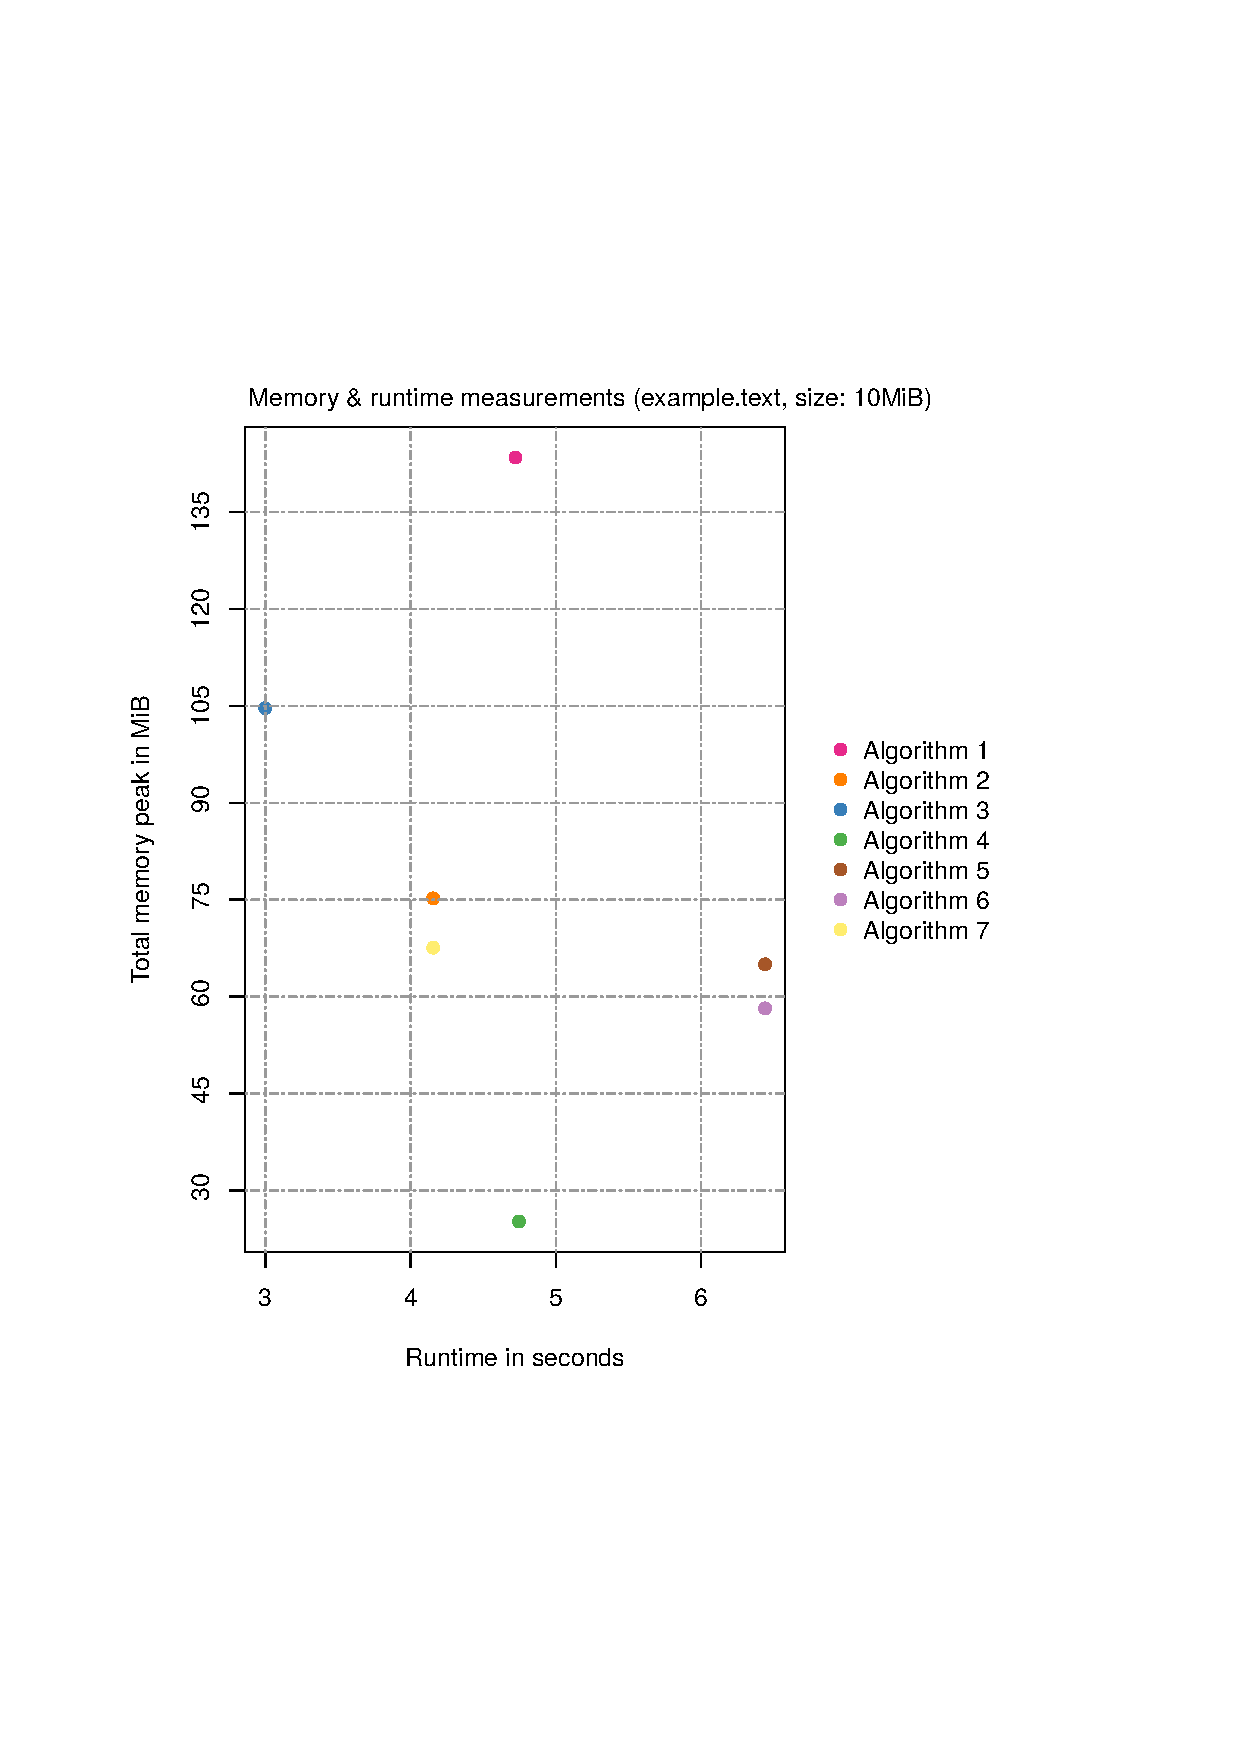
\includegraphics[page = 1, width=.5\textwidth]{kapitel/3_framework/benchmark/sacabench-batch/beispiel_batch_streu.pdf}
	\caption{Messergebnisse mehrerer Algorithmen}
	\label{pdf:benchmark:batch:streu}
\end{wrapfigure}

Die \cref{pdf:benchmark:batch:streu} zeigt die vierte Seite der \texttt{PDF}-Datei. Auf dieser ist statt eines Säulendiagramms ein Streudiagramm zum Einsatz gekommen. Hierbei handelt  es sich lediglich um eine andere Darstellungsform. Auf der X-Achse befindet sich die Skala für die Laufzeit und auf der Y-Achse die Skala für den maximalen Spei\-cher\-ver\-brauch von jedem Algorithmus für einen gegebenen Text. Rechts neben dem Diagramm ist die dazugehörige Legende wiederzufinden.

Auf der fünften Seite ist erneut ein Streudiagramm zu sehen. Jedoch ist dieses Mal lediglich die Pareto-Front eingezeichnet. Kurz und allgemein ausgedruckt gehört ein Punkt zu einer Pareto-Front, wenn kein anderer Punkt in allen Dimensionen \glqq besser\grqq{} ist.
In unserem Fall bedeutet das, dass ein zwei-dimensionaler Punkt dem Messergebnis eines Algorithmus entspricht, wobei eine Dimension der Laufzeit und die andere Dimension dem maximalen Spei\-cher\-ver\-brauch entspricht. Ein Algorithmus gehört somit zu der Pareto-Front, wenn kein anderer Algorithmus sowohl eine kürzere Laufzeit als auch einen kleineren maximalen Spei\-cher\-ver\-brauch aufweist. In \cref{pdf:benchmark:batch:streu} wären somit die Algorithmen \texttt{Algorithm 3} (blau), \texttt{Algorithm 4} (grün) und \texttt{Algorithm 7} (gelb) in der Pareto-Front.
Ein Diagramm, die die Pareto-Front abbildet, ist für eine Auswertung geeignet, da sich somit besser abschätzen lässt, welche Algorithmen sich für welche Problemstellungen am besten eignen.

Auf der sechsten Seite befindet sich ebenfalls ein Streudiagramm. Dieses hat allerdings logarithmische Skalen, sodass die Unterschiede der Messungen einfacher zu erkennen sind. Weisen zum Beispiel viele verschiedene Algorithmen ähnliche Mess\-er\-geb\-nisse auf, so werden die Unterschiede in logarithmischen Skalen größer dargestellt und es lassen sich somit gegebenenfalls eindeutigere Aussagen treffen.

Auf der siebten und somit letzten Seite ist erneut das \texttt{experimental setup} wiederzufinden mit zum Beispiel Angaben über den verwendeten Ar\-beits\-spei\-cher und Prozessor während der Ausführungen der Algorithmen.
\subsection{Automatische PDF-Generierung mit SqlPlotTools}
\label{framework:bechmark:sqlplottools}

\currentauthor{David Piper und Florian Grieskamp}
Wird \texttt{sacabench construct} zur Analyse eines einzelnen Algorithmus und dessen Phasen oder \texttt{sacabench batch} zum Vergleich mehrerer Algorithmen untereinander mit zusätzlicher Option \texttt{-{}-latexplot} ausgeführt, werden die erhaltenen Messdaten direkt in einer PDF-Datei aufgearbeitet.
Hierzu wird zunächst vom \texttt{sacabench} Haupttool eine Konfigurations-Datei mit Metainformationen über die durchgeführte Messung erstellt.
Diese beinhaltet Informationen zum System, auf dem die Analyse ausgeführt wird und zu dem Text, welcher als Input für die Algorithmen verwendet wurde.
Zum System werden die Anzahl der CPUs, die Anzahl an Threads pro Socket, das Modell und das verwendete Betriebssystem erfasst.
Bezüglich des Textes enthält die Konfigurationsdatei den Dateinamen des Textes, Präfixgröße und Anzahl der Wiederholungen der Messung.
Diese Datei wird im JSON-Format im Verzeichnis \texttt{zbmessung/sqlplot} gespeichert, welches ebenfalls ein Skript names automation.sh beinhaltet.\par
Im Anschluss an das Benchmarktool wird dieses Skript ausgeführt.
Hierdurch wird zunächst ein temporäres Verzeichnis erzeugt, welches zur Generierung der fertigen PDF-Dateien dient.
Neben der zuvor erstellten Konfigurations-Datei beinhaltet dieses Verzeichnis auch zwei LaTeX-Dateien, welche als Vorlagen für die zu erstellende PDF-Datei dienen, das für die Konvertierung des Datenformats benötigte Python-Skript \texttt{json\_to\_result\_converter.py} und ein Makefile, welches spätere Abläufe koordiniert.
Zusätzlich wird die JSON-Datei, welche bei der Messung durch das Benchmarktool erstellt wurde, in das temporäre Verzeichnis kopiert.
Damit sind alle benötigten Vorbereitungen getroffen und das Makefile im Unterverzeichnis \texttt{sqlplot} wird durch das Skript ausgeführt.\par\smallskip
Das Makefile führt das Python-Skript \texttt{json\_to\_result\_converter.py} aus, welches als erstes die Messergebnisse unter Berücksichtigung der Metadaten in ein \texttt{RESULT}-Format konvertiert.
Dieses beinhaltet die Daten in einem für \emph{SqlPlotTools} \cite{sqlplottools} lesbaren Format.
Da abhängig davon, ob \texttt{construct} oder \texttt{batch} aufgerufen wurde, unterschiedliche Daten im PDF benötigt werden, werden zwei unterschiedliche Result-Dateien erstellt:
Eine Datei enthält Daten für die genauere Analyse der unterschiedlichen Phasen aller Algorithmen und die andere Datei beinhaltet die Messwerte für gesamte Algorithmen.
Die Daten der einzelnen Phasen werden für die von \texttt{sacabench construct} erzeugten Diagramme benötigt, während die Messwerte der gesamten Algorithmen in den von \texttt{sacabench batch} erzeugten Diagrammen visualisiert werden.
Zusätzlich generiert das Python-Skript die LaTeX-Dateien, aus denen im Anschluss die fertigen PDF-Dateien erzeugt werden. 
Hierzu werden die beiden LaTeX-Vorlagen im Unterordner \texttt{templates} genutzt.
Nachdem all diese Dateien generiert wurden, klont das Makefile (sofern noch nicht im Verzeichnis \texttt{zbmessung/sqlplot} vorhanden) das SqlPlotTools-Repository von GitHub \cite{sqlplottools} in den temporären Ordner und baut dort das Projekt.
Jede durch das Python-Skript erstellte LaTeX-Datei wird durch einen Aufruf des SqlPlotTools mit den für die Plots benötigten Daten befüllt.
Dieser Aufruf wird ebenfalls von dem Makefile ausgelöst. 
Daraufhin können die LaTeX-Dateien gesetzt werden, wodurch die fertige PDF-Datei mit den neuen Messdaten entsteht.\par\smallskip
Im Anschluss kopiert das Skript \texttt{automation.sh} die generierte PDF-Datei in ihr Zielverzeichnis.
Zuletzt wird das temporäre Verzeichnis wieder vom System entfernt.
\newcommand{\comment}[1]{}
\comment{
In sacabench.cpp:
1. Erstellung einer Config-Datei mit Metainformationen über die durchgeführte Messung.
2. Speichern der Config-Datei in dem Ordner zbmessung/sqlplot.
3. Starte das Script zbmessung/automation.sh.

In zbmessung/automation.sh:
1. Erstelle temporären Ordner
2. Kopiere Ordner zbmessung/sqlplot in temporären Ordner
3. Kopiere durch Benchmark erstellte JSON-Datei in temporären Ordner
4. Rufe make im temporären Ordner auf.
5. Kopiere generierte PDF-Dateien an Zielort.
6. Lösche temporären Ordner.

Im temporären Ordner durch das Makefile:
1. Das Python-Skript json\_to\_result\_converter.py erstellt Result-Dateien, die von SqlPlotTools verarbeitet werden können. 
Diese enthalten die Daten aus der durch sacabench.cpp erstellten Config-Datei und der durch das Benchmark erstellten und durch automation.sh kopierten JSON-Datei mit den Messergebnissen.
Dazu werden zwei verschiedene Result-Dateien erstellt, eine mit Daten für den Vergleich mehrerer Algoirhtmen untereinander nach batch, und eine mit Daten für die genauere Analyse der einzelnen Phasen eines einzelnen Algorithmus nach construct.
Dieses Python-Skript generiert neben den Result-Dateien auch die LaTeX-Dateien, welche durch SqlPlotTools mit den Daten aus der Result-Datei befüllt werden.
Im Unterordner templates befinden sich zwei LaTeX-Dateien, eine für das Ergebnis eines construct-Aufrufs und eine für das Ergebnis eines batch-Aufrufs.
Abhänig vom Befülle die im Ordner templates befindlichen LaTeX-Dateien (je nach Ausführung) mit den Ergebnissen der Abfragen aus SqlPlotTools.
2. Klone SqlPlotTools von GitHub und baue das Projekt.
3. Jede durch das Python-Skript erstellte LaTeX-Datei wird durch einen Aufruf des SqlPlotTools mit Daten befüllt.
Dieser Aufruf wird ebenfalls von dem Makefile ausgelöst. 
4. Nachdem nun die LaTeX-Dateien generiert und mit den Daten befüllt sind, werden sie gesetzt.
}


\section{Code Struktur/Übersicht}
\label{sec:code-structure}
Dieses \currentauthor{David Piper und\\ Florian Grieskamp} Projekt besteht aus den vier Bereichen \textit{Bigtest}, \textit{External}, \textit{Sacabench} und \textit{Tests}. \par
Werden die Bigtests ausgef{\"u}hrt, werden verschiedene gro{\ss}e Textdateien geladen und lokal in dem Ordner external/datasets/downloads gespeichert. 
Anschlie{\ss}end werden die SACAs mit den gro{\ss}en Textdateien ausgef{\"u}hrt und das Ergebnis auf Korrektheit {\"u}berpr{\"u}ft. 
Die Ausf{\"u}hrung wird mit \termfont{make bigtest} gestartet. \par
Im Bereich External liegen verschiedene Bibliotheken, welche innerhalb des Projekts eingebunden werden.
Au{\ss}erdem sind die Referenzimplementierungen der SACAs im Unterordner reference\_impls enthalten. 
Diese k{\"o}nnen vom Framework mit Hilfe von Wrappern verwendet werden, welche sich im Bereich Sacabench befinden.
In dem Unterordner datasets/downloads sind zudem alle Texte enthalten, auf denen die Bigtests ausgef{\"u}hrt werden. \par
Sacabench ist der Hauptbestandteil des Frameworks. 
Im Ordner saca sind die Implementierungen der SACAs enthalten. 
Zus{\"a}tzlich befindet sich hier der Ordner external, in dem die zuvor beschriebenen Wrapper zur Einbindung der externen Referenzimplementierungen vorhanden sind. 
Alle SACAs enthalten die Wert \termfont{EXTRA\_SENTINELS}, \termfont{NAME} und \termfont{DESCRIPTION}. 
\termfont{EXTRA\_SENTINELS} bestimmt die Anzahl der zus{\"a}tzlichen Sentinals, die von dem Framework vor Aufruf des Algorithmus an den zu verarbeitenden Text angehangen werden m{\"u}ssen. 
\termfont{NAME} und \termfont{DESCRIPTION} werden bei Aufruf von \termfont{sacabench list} ausgegeben. 
Zus{\"a}tzlich stellt jeder SACA die Methode \termfont{construct\_sa} bereit, welche den Algorihtmus auf den {\"u}bergebenene Text anwendet. 
Die Wrapper stellen diese Werte f{\"u}r die externen Referenzimplementierungen bereit.
Neben dem Ordner saca befindet sich der Ordner util. 
In diesem sind verschiedenen Hilfsfunktionen und -klassen implementiert, beispielsweise finden sich hier unterschiedliche Sortieralgorithmen, die von den SACAs verwendet werden. 
Zuletzt befindet sich hier die Datei sacabench.cpp, welche das CLI implementiert. 
Sie enth{\"a}lt die main-Funktion, welche die eingegebenen Parameter verarbeitet und die ausgew{\"a}hlten Algorithmen startet.\par
Der Ordner Tests umfasst eine Menge von Testf{\"a}llen, welche mit \termfont{make check} ausgef{\"u}hrt werden k{\"o}nnen. 
Neben den Tests f{\"u}r die einzelnen Util-Klassen und -Funktionen stellt die Datei saca.hpp viele verschiedene Testeingaben bereit, mit denen die Korrektheit der internen und externen SACAs {\"u}berpr{\"u}ft werden kann. 
Anschlie{\ss}end wird das Ergebnis mit einem Referenz-SACA verglichen. 
Die Testeingaben, auf die die SACAs angewendet werden, umfassen verschiedene Sprachen und Zeichens{\"a}tze, u.a. einen All-a-Text, Smileys, Kanji und Hieroglyphen.\par


\chapter{Komponenten}
Viele \currentauthor{Rosa Pink} SACAs nutzen identische (oder zumindest ähnliche) Techniken oder Sortieralgorithmen. Daher ist es sinnvoll, diese Komponenten nicht mehrfach zu implementieren, sondern auf eine gemeinsame Implementierung zurückgreifen zu können, die dann von allen Algorithmen genutzt werden kann. Diese gemeinsamen Bestandteile werden hier nun beschrieben und definiert, sowie Besonderheiten bei der Implementierung hervorgehoben.

\section{Sortieralgorithmen}
\label{section:sortieralgorithmen}
\subsection{Quicksort}
\label{section:quicksort}

Der \currentauthor{Nico Bertram} Quicksort ist ein Sortieralgorithmus,
der nach dem Teile \& Herrsche Prinzip funktioniert und
in der ersten Version von Hoare vorgestellt wurde~\cite{quicksort}.
Der Algorithmus erreicht zwar mit $\mathcal O(n^2)$ im Gegensatz zu anderen
vergleichsbasierten Sortieralgorithmen eine schlechtere Worst-Case Laufzeit,
aber in der Praxis ist Quicksort besser als andere Algorithmen.

Das Vorgehen ist dabei wie folgt: Sei $A$ das zu sortierende Array.
Es wird ein geeignetes Pivotelement $p$ bestimmt und das Array durch Vertauschungen in
zwei Bereiche $A_{\text{left}}$ und $A_{\text{right}}$ aufgeteilt.
Dabei soll für alle $i$ gelten, dass $A_{\text{left}}[i] \le p$ und $A_{\text{right}}[i] > p$.
Die beiden Teilarrays werden anschließend rekursiv sortiert.
Der Rekursionsabbruch erfolgt, wenn das Eingabearray eine Größe von $0$ oder $1$ besitzt.
In diesen Fällen ist die Eingabe bereits sortiert.

Im Folgenden stellen wir mit Ternary Quicksort eine weitere Variante des Quicksort vor.
Anschließend beschreiben wir wie möglichst effizient das Pivotelement gewonnen werden kann.

\begin{listing}[!h]
    \begin{minted}{python}
    def bentley_mcilroy_tq(A: Array<SuffixStartPos>):
      if |A| > 1:
        p := choose a pivot element
    
        # Rearrange A so, that every element in A[0, left) is
        # smaller than p, every element in A[left, right) is equal
        # to p and every element in A[right, |A|) is greater than p.
        left, right := partition(A, p)
    
        bentley_mcilroy_tq(A[0, left))
        bentley_mcilroy_tq(A[right, |A|))
    \end{minted}
    \caption{Bentley-McIlroy ternäres Quicksort~\cite{ternary_quicksort}}
\end{listing}    

\subsubsection{Ternary Quicksort}
\label{section:ternary_quicksort}

\noindent
Ternary Quicksort ist eine Variante des Quicksort, die besonders geeignet ist,
wenn in der Eingabe mehrere gleiche Elemente vorkommen~\cite{ternary_quicksort}.
Wir wählen hier wieder ein geeignetes Pivotelement $p$.
Statt die Eingabe in zwei Bereiche aufzuteilen, teilen wir die Eingabe in drei Bereiche $A_{\text{left}}$, $A_{\text{middle}}$ und $A_{\text{right}}$ auf (siehe \cref{fg:ternary_partitions}).
In $A_{\text{left}}$ sind alle Elemente enthalten, die echt kleiner sind als $p$.
In $A_{\text{middle}}$ sind alle Elemente enthalten, die gleich $p$ sind, und in $A_{\text{right}}$ sind alle Elemente enthalten, die größer als $p$ sind.
Die Größe dieser Bereiche lässt sich durch Zählen der Elemente bestimmen.
Anschließend können die Elemente durch Vertauschen in den richtigen Bereich geschrieben werden.

Nachdem wir alle Elemente in die drei Bereiche aufgeteilt haben, müssen $A_{\text{left}}$ und $A_{\text{right}}$ rekursiv sortiert werden.

\begin{figure}[!h]
	\centering
	\begin{tikzpicture}
	\draw (0,0) -- (10,0) -- (10,1) -- (0,1) -- cycle;
	\draw (3,0) -- (3,1);
	\draw (8,0) -- (8,1);
	
	\node at (1.5, 0.5) {<};
	\node at (5.5, 0.5) {=};
	\node at (9, 0.5) {>};
	
	\draw[red] (6,0.5) -- (6,2) node[above] {\texttt{p}};
	
	\begin{scope}[yshift=-10pt]
	\draw[decorate, decoration={mirror, brace,amplitude=10pt}] (0.1,0) -- (2.9,0) node[midway, below = 10pt] {$A_\text{left}$};
	\draw[decorate, decoration={mirror, brace,amplitude=10pt}] (3.1,0) -- (7.9,0) node[midway, below = 10pt] {$A_\text{middle}$};
	\draw[decorate, decoration={mirror, brace,amplitude=10pt}] (8.1,0) -- (9.9,0) node[midway, below = 10pt] {$A_\text{right}$};
	\end{scope}
	\end{tikzpicture}
	\caption[Partitionen bei ternärem Quicksort]{Partitionen bei ternärem Quicksort. (Abbildung ähnlich in \cite{ternary_quicksort}.)}
	\label{fg:ternary_partitions}
\end{figure}

\subsubsection{Auswahl des Pivotelements}

Es gibt unterschiedliche Ansätze in den hier beschriebenen Quicksort-Varianten das Pivotelement zu wählen.
Das Problem ist der Trade-Off zwischen aufwändiger Pivot-Wahl (Pivotwahl hat hohe Laufzeit) und
degeneriertem Quicksort durch eine schlechte Wahl des Pivotelements (Quicksort hat hohe Laufzeit).

Einfache Ansätze sind es das erste, mittlere oder das letzte Element der Eingabe zu wählen.
Diese Ansätze sind problematisch wenn das gewählte Pivotelement ein sehr kleines oder ein sehr großes Element ist.
Dadurch wird die Eingabe nicht in zwei annähernd gleich große Bereiche aufgeteilt und die rekursiven Aufrufe werden ineffizient (degeneriertes Quicksort).

Daher verwenden wir im Quicksort und im Ternary Quicksort eine verbesserte Variante~\cite{ternary_quicksort}.
Falls die Größe des Eingabearrays kleiner als ein bestimmter Threshold ist,
bestimmen wir den \emph{Median of 3}. Das bedeutet, dass wir uns das erste,
das mittlere und das letzte Element der Eingabe anschauen und den Median von diesen drei Elementen wählen.
In der Implementierung haben wir als Threshold $40$ gewählt.
Falls die Größe des Eingabearrays größer als als der gewählte Threshold ist,
bestimmen wir den \emph{Median of 9}. Dazu teilen wir das Array in drei gleich große Teilarrays auf
und bestimmen für jedes dieser Teilarrays den \emph{Median of 3}.
Unter diesen drei Elementen wird wiederum der Median gebildet, um das Pivotelement zu erhalten.
\subsection{Introsort}
\label{section:introsort}

Nicht \currentauthor{Oliver Magiera} immer kann eine Laufzeit von $\mathcal O(n\log{n})$ beim Quicksort garantiert werden.
Für diesen Zweck wurde der Introsort Algorithmus (auf Basis des binären Quicksort) entworfen \cite{Musser97}:
nach einer Rekursionstiefe $h$ durch den Quicksort Algorithmus wird Heapsort verwendet,
um ein Teilarray \textbf{A'} von \textbf{A} endgültig zu sortieren.
Als Wert für die maximale Tiefe $h$ hat sich $2 \lfloor \log_2{|A|}\rfloor$ als empirisch geeignet herausgestellt.
Eine weitere Optimierung liegt in der Verwendung von Insertionsort,
wenn die Anzahl der Elemente einen Schwellwert $\theta$ unterschreitet.

\begin{figure}
\begin{minted}[escapeinside=||, linenos=true, autogobble]{python}
def introsort(A: Array<Integer>, f: Integer, b: Integer):
  introsort_loop(A, f, b, |$2 \lfloor \log_2{(b-f)}\rfloor$|)
  insertionsort(A, f, b)
\end{minted}

\begin{minted}[escapeinside=||, mathescape=true, linenos=true, autogobble]{python}
def introsort_loop(A: Array<Integer>, f: Integer, b: Integer, depth_limit: Integer)
  while b - f > |$\theta$|
    if depth_limit == 0
      heapsort(A, f, b)
      return end
    depth_limit := depth_limit - 1
    p := Choose pivot element

    # Rearrange A such that all elements $\leq$ p are in $A[f\dots i]$
    # and all elements > p in A$[i\dots b]$
    i := partition(A, f, b, p)
    # Recursively sort >-Partition
    introsort_loop(A, i, b, depth_limit)
    # Sort left partition ($\leq$) in next iteration
    b := i

\end{minted}
\caption{Introsort mit \glqq $\leq$\grqq- und \glqq >\grqq-Partition.}
\label{alg:introsort}
\end{figure}

Der Pseudocode in \ref{alg:introsort} beschreibt den Ablauf des Algorithmus\todo{referenz hinzufügen}.
Dabei befindet sich in \texttt{introsort\_loop} die eigentliche Funktion: In Zeile 3 wird geprüft,
ob die Größe des (Teil-)Arrays den Schwellwert unterschreitet. Ist dies der Fall, bricht die Rekursion ab.
Andernfalls muss geprüft werden, ob die maximale Tiefe bereits erreicht wurde.
Falls ja, wird das (Teil-)Array vollständig mit Heapsort sortiert.
Tritt dies ebenfalls nicht ein, wird die verbleibende Rekursionstiefe um eins reduziert,
das Pivotelement bestimmt und das Array anhand dessen partitioniert,
d.h. alle größeren Elemente landen in der rechten Partition, alle Anderen in der Linken.
Zuletzt wird rekursiv \texttt{introsort\_loop} auf die rechte Partition ausgeführt
und danach die rechte Grenze $b$ auf die linke Partition angepasst, welche iterativ weiter sortiert wird.

Die Methode \texttt{introsort} ruft \texttt{introsort\_loop} mit dem übergebenen Anfang $f$ und Ende $b$ sowie
mit der empirisch geeigneten Maximaltiefe aufgerufen. Daraufhin wird Insertionsort auf das übergebene Array ausgeführt.
Durch die vorige Vorverarbeitung über die innere Introsort-Schleife müssen nur noch Intervalle
der Länge $\leq \theta$ final sortiert werden.
Dies funktioniert deshalb effizient, da z.~B. Elemente im Intervall $[0, \theta)$ noch nicht
endgültig sortiert sind, sie befinden sich jedoch bereits im richtigen Intervall.
Somit wird kein Element aus $[\theta, 2 \theta)$ oder einem hinteren Intervall in \textbf{A} kleiner
sein als ein beliebiges Element aus dem Intervall $[0,\theta)$.

\subsection{Multikey-Quicksort}
\label{section:mkqs}
Der \currentauthor{Oliver Magiera und Marvin Böcker} Multikey-Quicksort von
Bentley und Sedgewick~\cite{multikey_quicksort} basiert auf ternary Quicksort (siehe \cref{section:ternary_quicksort})
und sortiert Strings eines Arrays \textsf{A} zeichenweise.
Das Funktionsargument $d$ beschreibt, welches Zeichen momentan verglichen werden soll.
Initial ist dieser Parameter $d = 0$,
um das erste Zeichen von den Strings in \textsf{A} zu vergleichen.
Wenn dieses Zeichen kleiner oder größer ist,
kann der String in die \glqq <\grqq- bzw \glqq >\grqq-Partition sortiert werden.

\begin{figure}
	\begin{minted}[mathescape=true,escapeinside=||]{python}
def mkqs(A: Array<SuffixStartPos>, d: Integer):
  if |A| <= 1:
    return end

  p := choose a pivot element

  # Rearrange A so, that T[A[..i]] has a character at position d
  # that is smaller than p, T[A[i..j]] has p at position d and 
  # T[A[j..]] has a character at position d that is larger than p.
  i, j := partition(A, d, p)

  mkqs(A[0, i), d)
  # Sort Equal-Partition by next character.
  mkqs(A[i, j), d+1)
  mkqs(A[j, |A|), d)
	\end{minted}
	\caption{Bentley-Sedgewick Multikey-Quicksort~\cite{multikey_quicksort}.}
	\label{alg:mkqs}
\end{figure}

Bei Gleichheit hingegen muss das nächste Zeichen betrachtet werden, um die Strings eindeutig zu sortieren,
während für die \glqq <\grqq- bzw. \glqq >\grqq-Partitionen nach dem aktuellen Zeichen genauer sortiert wird.
Abbildung \ref{fg:ternary_partitions} stellt die Partitionierung eines Sortierschritts bei Pivotelement $p$ an.

Der Pseudocode \ref{alg:mkqs} skizziert die Vorgehensweise des MK-QS Algorithmus.
Es wird erst ein Pivotelement $p$ bestimmt, welches zur Partitionierung benötigt wird.
Dabei werden alle Elemente kleiner als das Pivot in $[0, i)$ einsortiert,
alle gleich dem Pivotelement in $[i, j)$ und schließlich alle größeren Elemente in $[j, |\textsf{A}|)$.
Zunächst wird die \glqq <\grqq-Partition nach dem $d$-ten Zeichen rekursiv weiter sortiert,
bevor für die \glqq =\grqq-Partition zum Sortieren das $d+1$-te Zeichen verwendet wird.
Zuletzt wird die Rekursion für die \glqq >\grqq-Partition durchgeführt.


\subsection{Bucketsort}
\label{section:bucketsort}

Der \currentauthor{Florian Grieskamp} Bucketsort-Algorithmus \cite[Kapitel 8.2 (dort unter dem Namen \emph{counting sort})]{Cormen2009} ist ein Sortierverfahren, das für Werteverteilungen über einem Alphabet einer konstanten Größe Eingaben in linearer Zeit sortieren kann. Da die Bedingung einer konstanten Alphabetgröße allerdings häufig nicht erfüllt ist, wird Bucketsort oft in Verbindung mit einer Schlüsselfunktion verwendet, um gemäß des Schlüssels \glqq ähnliche\grqq{} Werte zu gruppieren. Diese gruppierten Bereiche werden als \emph{Buckets} bezeichnet und im Anschluss mit einem anderen Sortierverfahren verfeinert. Bucketsort dient in dieser Variante als Mechanismus zur groben Vorsortierung.\par
\todo{Das sollte in der Notation schon sein. (mb)}
\begin{definition}[Bucket]
	\label{def:bucket}
	Ein Intervall \(\bucket{} \coloneqq \sa[l, r]\) des Suffix-Arrays begrenzt durch einen linken Index \(l\) und einen rechten Index \(r\) heißt Bucket.\par
    Falls alle in einem Bucket \(\bucket{p} \coloneqq \sa[l, r]\) enthaltenen Suffixe, also die Suffixe \(\suffix{\sa[l]}, \suffix{\sa[l+1]}, \ldots, \suffix{\sa[r]}\), einen gemeinsamen Präfix \(p\) der Länge \(m\) haben, so heißt \(\bucket{p}\) Level-\(m\)-Bucket.
\end{definition}
Da im Anwendungsfeld der Suffix-Array-Konstruktion die zu sortierenden Elemente Suffixe über \(\Sigma^\ast\) sind, ist eine Schlüsselfunktion notwendig, die Wertebereich einschränkt. Hier werden als Schlüssel gemeinsame Präfixe der Länge \(d\) (für Bucketsort mit Tiefe \(d\)) verwendet.\par
Der Algorithmus besteht aus drei iterativ durchgeführten Schritten, die hier erläutert werden. Als begleitendes Beispiel dient die Sortierung der Suffixe des Wortes \emph{caabaccaabacaa} mit der Tiefe 2.
\paragraph{Schritt 1}
Es wird zunächst ein Hilfs-Array (\cref{bucketsort:bkt}) angelegt, in dem zu jedem möglichen Schlüssel (hier Präfixe über \(\Sigma^2\)) dessen Häufigkeit in der Eingabe vermerkt wird. Dies geschieht anhand eines sequentiellen Scans der Eingabesequenz. Diese Anzahl legt die Größe des jeweiligen Buckets fest. In einem Scan des Hilfs-Arrays kann dann In-Place die kumulative Summe der Größen bestimmt werden, durch welche die Grenzen zwischen den Buckets festgelegt werden.
\begin{figure}[ht]
    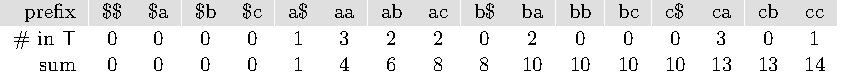
\includegraphics[width=\textwidth]{kapitel/4_komponenten/sortieralgorithmen/bucketsort/step_01/bkt/image.pdf}
    \caption{Bestimmung der Bucketgrößen und Startpositionen}
    \label{bucketsort:bkt}
\end{figure}
\paragraph{Schritt 2}
Um die Elemente sortieren zu können, wird ein zweites Array in der Länge der Eingabesequenz angelegt. Dieses Array ist auf Basis der zuvor berechneten Grenzen (imaginär) in Buckets eingeteilt (\cref{bucketsort:empty_buckets}).
\begin{figure}[ht]
    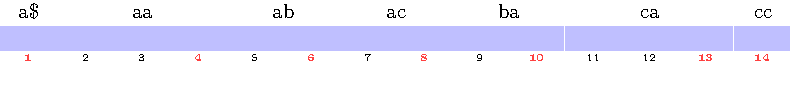
\includegraphics[width=\textwidth]{kapitel/4_komponenten/sortieralgorithmen/bucketsort/step_02/empty_buckets/image.pdf}
    \caption{Buckets ohne einsortierte Suffixe}
    \label{bucketsort:empty_buckets}
\end{figure}
In einem Scan der Eingabesequenz wird dann iterativ für jedes Element der zugehörige Schlüssel berechnet, um anhand der Tabelle aus \cref{bucketsort:bkt} die Position im Ausgabe-Array zu bestimmen. Nach dem Einfügen an dieser Position wird die Grenze des jeweiligen Buckets entsprechend angepasst, um bereits eingefügte Elemente im Nachhinein nicht mit neuen Elementen zu überschreiben.\par
Nach Abschluss dieses Schritts liegen die vorsortierten Elemente der Eingabesequenz in korrekter Reihenfolge bezüglich des gewählten Sortierschlüssels im Ausgabe-Array (\cref{bucketsort:buckets}).
\begin{figure}[ht]
    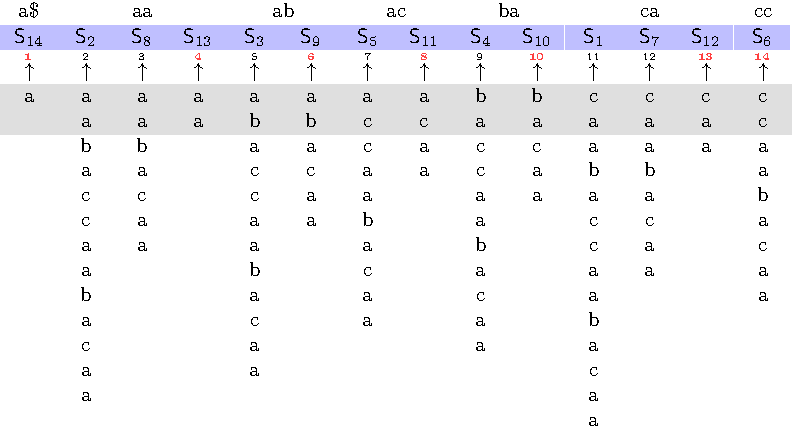
\includegraphics[width=\textwidth]{kapitel/4_komponenten/sortieralgorithmen/bucketsort/step_02/buckets/image.pdf}
    \caption{Buckets mit einsortierten Suffixen}
    \label{bucketsort:buckets}
\end{figure}
\paragraph{Schritt 3 (optional)}
Je nach Anwendungsfall kann es erwünscht sein, dass die Elemente in sortierter Reihenfolge direkt im Eingabe-Array liegen. Falls dies erforderlich ist, so wird in einem dritten Scan der Inhalt des Ausgabe-Arrays ins Eingabe-Array kopiert und dabei die alte Eingabe überschrieben. Die Weiterverarbeitung der einzelnen Buckets erfolgt dann mit einem anderen Sortieralgorithmus oder wahlweise auch weiter mit Bucketsort unter Verwendung einer anderen Schlüsselfunktion.

\subsection{Radixsort}
\label{sort:radix}

In \currentauthor{Nico Bertram} diesem Abschnitt behandeln wir das Sortierverfahren \emph{Radixsort}.
Dabei handelt es sich im Gegensatz zu den anderen Sortieralgorithmen, die in unserem Framework verwendet werden,
nicht um einen vergleichsbasierten Sortieralgorithmus.
Es werden stattdessen die einzelnen Stellen der zu sortierenden Elemente $A$ in einer bestimmten Reihenfolge sortiert.
Die Stellen der Elemente sind dabei Zeichen aus einem endlichen Alphabet.
Da wir die Größe des Alphabets im Voraus kennen, lassen sich die Elemente in Buckets einsortieren.
Wenn die maximale Anzahl der Stellen der Elemente $k$ beträgt,
erreicht dieser Algorithmus eine Worst-Case Laufzeit von $\mathcal O(kn)$.
Falls $k$ konstant ist, ist die Laufzeit somit linear.

Wir stellen in diesem Abschnitt verschiedene Radixsort-Varianten vor.
Zum einen unterscheiden sich diese hinsichtlich der Reihenfolge,
in der die Stellen der Elemente betrachtet werden.
Es kann bei der Stelle mit der höchsten Wertigkeit (MSD) oder der Stelle mit der niedrigsten Wertigkeit (LSD) begonnen werden.
Wenn wir die Elemente nach dem MSD sortieren sind die Elemente nach den Zeichen an der aktuell betrachteten Stelle vorsortiert.
Um Elemente mit gleichen Zeichen zu sortieren, müssen die übrigen Stellen rekursiv sortiert werden.
Wenn wir die Elemente nach dem LSD sortieren,
müssen die Elemente nach der aktuell betrachteten Stelle so in die Buckets einsortiert werden,
dass bei gleichem Zeichen an der aktuellen Stelle die bisherige Sortierung erhalten bleibt.
Beide Radixsort-Varianten wurden unter anderem auch in \cite{Cormen2009} beschrieben.

Außerdem lässt sich Radixsort mit einem zusätzlichen Hilfsarray oder inplace sortieren.
Die Varianten, die ein zusätzliches Hilfsarray benötigen, sind stabile Sortierverfahren.
Die inplace Varianten sind instabile Sortierverfahren.

In allen Varianten, die wir hier vorstellen,
muss als Eingabeparameter eine \texttt{key\_function} übergeben.
Dies ist eine Funktion, die als Eingabe ein Element des Eingabearrays und die aktuelle Stelle erhält,
und das Zeichen des Elements an der aktuellen Stelle zurückgibt.
Dies ist von Vorteil, wenn die Eingabearrays unterschiedliche Formen besitzen.
Es kann sein, dass die Eingabe aus den tatsächlich zu sortierenden Elementen besteht,
oder die Eingabe besteht wie im \cref{algorithm:nzSufSort} aus Positionen von Teilstrings im Eingabetext.

Die unterschiedlichen Radixsort-Varianten verwenden alle die Hilfsfunktion \emph{Bucketsort} (siehe \cref{section:bucketsort}).
Diese erhält als Eingabe die zu sortierenden Elemente $A$, die aktuelle Stelle $i$ und ein Bucketarray
$B$ mit $|B| = |\Sigma|$. \emph{Bucketsort} zählt zu jedem Zeichen des Alphabets die Häufigkeit
und speichert diese in $B$.
Anschließend werden die Elemente von $B$ von links nach rechts aufsummiert,
wobei das erste Element die $0$ erhält.
Dadurch werden in $B$ die Startpositionen der jeweiligen Buckets berechnet.

\subsubsection{MSD-Radixsort}
\label{sort:radix:msd}

Diese Variante sortiert die Elemente beginnend ab dem MSD und verwendet ein zusätzliches Hilfsarray $R$.
Zunächst werden mit \emph{Bucketsort} in ein Bucketarray $B$ der Größe $|\Sigma|$ die Startpositionen
der Buckets berechnet. Anschließend werden die Elemente anhand der Zeichen in die Buckets aufgeteilt.
Dazu bestimmen wir mithilfe von $B$ die Position, an der wir das Element in $R$ schreiben müssen und
inkrementieren anschließend die entsprechende Position von $B$.
Nachdem alle Elemente in $R$ geschrieben wurden, werden diese wieder zurück in das Eingabearray kopiert.
Falls es Buckets gibt, die mehr als ein Element enthalten, werden diese Buckets rekursiv mit der nächsten
Stelle weiter sortiert.

Im folgenden Beispiel werden die Elemente $A=\{512, 794, 187, 394, 384\}$ mit MSD-Radixsort sortiert.
Dabei sortieren wir die Elemente zunächst nach der ersten Stelle. 

\begin{table}[H]
	\centering
	\begin{tabular}{c|| c | c c | c | c }
		$i$ & 0 & 1 & 2 & 3 & 4 \\
		$A[i]$ & 187 & 394 & 384 & 512 & 794
	\end{tabular}
	\label{tab:radix:msd:step_1}
\end{table}

Da das Bucket für das Zeichen $3$ mehr als ein Element enthält wird dieses rekursiv nach der zweiten Stelle sortiert.

\begin{table}[H]
	\centering
	\begin{tabular}{c|| c | c | c | c | c }
		$i$ & 0 & 1 & 2 & 3 & 4 \\
		$A[i]$ & 187 & 384 & 394 & 512 & 794
	\end{tabular}
	\label{tab:radix:msd:step_2}
\end{table}

Nun existiert kein Bucket mit mehr als einem Element. Die Eingabe wurde also sortiert.
An diesem Beispiel kann man einen Vorteil des MSD-Radixsort erkennen.
Man muss nicht jede Stelle betrachten, wenn die Eingabe bereits sortiert ist, und kann bereits vorher abbrechen.
Dadurch ist die Laufzeit in der Praxis schneller.
Jedoch muss für jeden rekursiven Aufruf das Bucketarray im Stack behalten werden.
Bei großen Alphabeten kann das zu großem Speicherverbrauch führen.

\subsubsection{LSD-Radixsort}
\label{sort:radix:lsd}

In dieser Variante werden die Elemente beginnend ab dem LSD sortiert.
Die Sortierung der Elemente anhand der aktuellen Schritte ist analog zum MSD-Radixsort.
Wenn wir eine Stelle weitergehen, müssen aber alle Elemente anhand der nächsten Stelle sortiert werden.

Im folgenden Beispiel sortieren wir erneut die Elemente $A=\{512, 794, 187, 394, 384\}$.
Dabei verwenden wir diesmal den LSD-Radixsort.
Wir beginnen mit der Sortierung an der letzten Stelle.

\begin{table}[H]
	\centering
	\begin{tabular}{c|| c | c c c | c }
		$i$ & 0 & 1 & 2 & 3 & 4 \\
		$A[i]$ & 512 & 794 & 394 & 384 & 187
	\end{tabular}
	\label{tab:radix:lsd:step_1}
\end{table}

Anschließend werden die Elemente nach der zweiten Stelle sortiert.
Dabei bleibt die Sortierung des vorherigen Schrittes bei gleichen Zeichen erhalten.

\begin{table}[H]
	\centering
	\begin{tabular}{c|| c | c | c | c | c }
		$i$ & 0 & 1 & 2 & 3 & 4 \\
		$A[i]$ & 512 & 384 & 187 & 794 & 394
	\end{tabular}
	\label{tab:radix:lsd:step_2}
\end{table}

Als Letztes sortieren wir die Elemente nach dem ersten Zeichen.
Anschließend sind die Elemente fertig sortiert.

\begin{table}[H]
	\centering
	\begin{tabular}{c|| c | c | c | c | c }
		$i$ & 0 & 1 & 2 & 3 & 4 \\
		$A[i]$ & 187 & 384 & 394 & 512 & 794
	\end{tabular}
	\label{tab:radix:lsd:step_3}
\end{table}

Im Gegensatz zum MSD-Radixsort reicht es hier aus nur ein Bucketarray im Speicher zu haben.
Diese Radixsort-Variante ist also speichereffizienter.
Da für die Sortierung jede Stelle berücksichtigt werden muss,
ist diese Variante in der Praxis aber langsamer als MSD-Radixsort.

\subsubsection{Inplace MSD-Radixsort}
\label{sort:radix:inplace}

Der MSD-Radixsort lässt sich so modifizieren, dass kein zusätzliches Hilfsarray benötigt wird \cite{radixsort:inplace}.
Statt die Elemente direkt in ihre richtige Buckets zu schreiben,
müssen wir durch Vertauschungen die Elemente an die richtige Position bringen.
Hier sei angemerkt, dass wir den LSD-Radixsort nicht auf die gleiche Art modifizieren können,
da die einzelnen Stellen stabil sortiert werden müssten.
Wenn wir Elemente miteinander tauschen würden, wäre diese Stabilität nicht mehr garantiert.

Wenn wir die Elemente im Eingabearray in die richtigen Buckets schreiben,
lassen sich die Elemente in zwei Mengen einteilen.
Es gibt Elemente, die bereits ins richtige Bucket geschrieben wurden,
und Elemente, die noch nicht in das richtige Bucket geschrieben wurden.
Wenn wir über die Elemente der Eingabe iterieren, müssen wir nur die Elemente betrachten,
die noch nicht in das richtige Bucket geschrieben wurden.
Die Anderen müssen wir überspringen.
Dazu benötigen wir zwei Bucketarrays $B_{\text{start}}$ und $B_{\text{end}}$.
In $B_{\text{start}}$ steht für jedes Zeichen des Alphabets die Startposition des jeweiligen Buckets drin
und in $B_{\text{end}}$ steht die erste freie Position des Buckets drin.
Da zu Beginn die Startpositionen und ersten freien Positionen eines Buckets zusammenfallen,
lassen sich $B_{\text{start}}$ und $B_{\text{end}}$ durch Bucketsort berechnen.

Um die Elemente in die Buckets aufzuteilen durchlaufen wir das Eingabearray von links nach rechts.
Wenn wir an der Position $i$ sind, schreiben wir $A[i]$ gemäß dem Zeichen $\sigma$ von $A[i]$ an der
aktuellen Stelle an die Position $j = B_{\text{end}}[\sigma]$.
Falls $i \ne j$ gilt, werden die Elemente an den Positionen $i$ und $j$ getauscht
und für den nächsten Schritt bleibt unser $i$ unverändert.
Falls $i = j$ gilt, bleibt $A[i]$ an der aktuellen Stelle stehen und unser $i$ muss erhöht werden.
Dabei müssen wir darauf achten, dass $i$ immer auf eine Position zeigt,
die noch nicht in ein Bucket einsortiert wurde.
Wir müssen also $i$ mit der Startposition $k$ des nächsten Buckets in $B_{\text{start}}$ vergleichen.
Falls $i+1 < k$, können wir $i$ inkrementieren.
Ansonsten müssen wir solange volle Buckets überspringen bis wir $i$ auf eine freie Position setzen können.

Falls es nach der Aufteilung Buckets gibt, die mehr als ein Element enthalten,
müssen diese rekursiv für die nächste Stelle sortiert werden.

\subsubsection{Radixsort für große Alphabete}
\label{sort:radix:big_alph}

Im Folgenden nehmen wir an, dass wir Elemente sortieren,
die aus maximal $3$ Zeichen bestehen. Dieses Vorgehen ließe sich aber auch für längere Elemente verallgemeinern.
In unserem Framework haben wir eine Radixsort-Variante entworfen, die sich besonders eignet,
wenn die Größe des Alphabets durch die Größe des Eingabearrays beschränkt ist.
Also für $n=|A|$ gilt $|\Sigma| \le n$. Die Variante, die wir in \cref{sort:radix:inplace} vorgestellt haben,
ist in diesem Fall nicht geeignet, da in jedem Rekursionsschritt ein neues Bucketarray erzeugt wird.
Dadurch kann sich ein Speicherverbrauch von $\mathcal O(3n)$ ergeben.

Wir beschreiben hier wie man die Variante aus \cref{sort:radix:inplace} so modifizieren kann,
dass wir genau mit einem Bucketarray $B$ der Größe $n$ auskommen können.
Die Idee ist es das Eingabealphabet in jedem rekursiven Schritt so zu verkleinern,
dass wir in allen rekursiven Schritten genug Platz in $B$ haben.

Dazu teilen wir das Eingabealphabet in fünf Buckets der Größe $\frac{n}{5}$ auf.
Jedes dieser Buckets wird nun wie in \cref{sort:radix:inplace} beschrieben in die Buckets für jedes Zeichen aufgeteilt.
Da wir nur noch $\frac{n}{5}$ der Zeichen sortieren müssen,
benötigt die Aufteilung für $B_{\text{start}}$ und $B_{\text{end}}$ jeweils nur $\frac{n}{5}$ Speicher.
Außerdem benötigen wir nach der Aufteilung nur $B_{\text{start}}$ für die rekursiven Aufrufe.
Das heißt es reicht aus für den ersten und zweiten rekursiven Aufruf jeweils $\frac{n}{5}$ Speicher zu verwenden
und für den dritten rekursiven Aufruf benötigen wir für $B_{\text{start}}$ und $B_{\text{end}}$
insgesamt $\frac{2n}{5}$ Speicher. Insgesamt passt also für jeden rekursiven Aufruf der verwendete Speicher in $B$.

\subsubsection{Optimierung}

Bei den MSD-Radixsort-Varianten ist es in der Praxis meistens nicht sinnvoll kleine Buckets
weiter mit Radixsort zu sortieren, da viele rekursive Aufrufe mit kleinen Bucketgrößen einen zu großen Overhead erzeugen.
In diesen Fällen ist es deutlich schneller ab einer bestimmten Bucketgröße die Buckets mit einem
naiven Sortieralgorithmus wie Insertionsort zu sortieren.
Dazu muss in diesen Radixsort-Varianten zusätzlich eine \texttt{compare\_function} übergeben werden,
die als Eingabe die zu vergleichenden Elemente $i$ und $j$ und die aktuelle Stelle $k$ erhält.
Die \texttt{compare\_function} vergleicht dann die Elemente, wobei die Zeichen, die vor der Stelle $k$ vorkommen,
abgeschnitten werden.
\subsection{Standardbibliothek-Sortierer}
\label{section:stdsort}

In \sacabench verwenden wir außerdem die Sortierer aus der GNU Standardbibliothek von C++.
Wir verwenden insbesondere die parallelen Varianten von \texttt{std::sort}
und \texttt{std::stable\_sort}.
Diese erwiesen sich als zuverlässiger als \ipsviero auf vielen Kernen
und werden daher für die naiven Parallelisierungen der SACAs verwendet.

Im nicht-stabilen Sortierer kann entweder \emph{Parallel Multiway Mergesort} oder \emph{Parallel Load-Balanced Quicksort} verwendet werden.
Die Mergesort-Variante teilt dabei das Problem nicht in zwei Teile sondern $k$ Teile, wovon jeder von einem anderen Kern bearbeitet wird.
Um Verlangsamungen durch kleine Partitionen zu vermeiden, teilt die Quicksort-Variante Threads,
die mit ihrem Anteil des Arrays schon fertig sind, neue Teile zu, um eine höhere Effizienz zu erreichen.
Da der erste Algorithmus stabil sortiert, wird er auch als stabiler Sortierer verwendet.
Die Details der verwendeten Algorithmen werden im Paper von Singler und Kosnik von 2008~\cite{parallelstdsort} erläutert.
\subsection{Inplace Parallel Super Scalar Samplesort (\ipsviero)}
\label{section:ips4o}

In \sacabench verwenden wir auch andere Sortieralgorithmen, die wir nicht selbst implementiert haben.
Der erste dieser Algorithmen ist \ipsviero~\cite{axtmann2017}.
Dieser existiert in einer sequentiellen und einer parallelen Variante,
die mittels OpenMP parallel funktioniert.

\ipsviero baut auf Samplesort auf, welcher wiederrum auf Quicksort aufbaut.
Statt nur ein Pivot wie bei Quicksort werden dabei aber mehrere Pivot verwendet.
Dadurch erhält man einen Algorithmus \glqq der cache-effizient ist, datenparallel arbeitet und \emph{branch mispredictions} verhindert\grqq~\cite{axtmann2017}.
\ipsviero verbessert diesen Algorithmus und implementiert ihn in-place, also mit $\mathcal O(1)$ Extraspeicher.
Da dies ein komplexes, vergleichsbasiertes Sortierverfahren ist,
sei an dieser Stelle für weitere Details auf das Paper von Axtmann et al.~\cite{axtmann2017}
beziehungsweise das öffentliche Repository von \ipsviero~\cite{ips4o:repo} verwiesen.
\subsection{Standardbibliothek-Sortierer}
\label{section:stdsort}

In \sacabench verwenden wir außerdem die Sortierer aus der GNU Standardbibliothek von C++.
Wir verwenden insbesondere die parallelen Varianten von \texttt{std::sort}
und \texttt{std::stable\_sort}.

\blindtext
\section{Techniken}
In diesem Kapitel stellen wir Techniken vor, die unabhängig vom Algorithmus genutzt werden können. Diese sollen die Berechnung des Suffix-Arrays vereinfachen und auch beschleunigen können. 
\subsection{Effektives Alphabet}
\label{section:effalphabet}
Sowohl \currentauthor{Hermann Foot} die Laufzeit als auch der Speicherverbrauch einiger der im Framework enthaltenen Algorithmen sind abhängig von der Alphabetgröße des gegebenen Strings. Da das Alphabet allerdings oft mehr Zeichen umfasst als tatsächlich im String vorkommen, kann es sinnvoll sein das vorliegende Alphabet auf die ausschließlich genutzten Zeichen zu reduzieren. Ein solches Alphabet nennen wir effektives Alphabet.\par
\begin{definition}[Effektives Alphabet]
	\label{def:effective_alphabet}
	Sei \(\effective : \Sigma \cup \{\$\} \rightarrow \{0, \ldots, |\Sigma|\}\) eine bijektive Funktion\footnote{\label{differs_from_paper}An dieser Stelle weicht die formale Definition bewusst von der in der zugehörigen Publikation \cite{saca:2} ab, um Definitionslücken für erweiterte Strings zu vermeiden.}, sodass
	\begin{enumerate}
		\item \(\effective(\$) = 0\) \quad und damit \(\forall c \in \Sigma : \effective(\$) < \effective(c)\) und
		\item \(\forall c_1, c_2 \in \Sigma : c_1 < c_2 \Rightarrow \effective(c_1) < \effective(c_2)\).
	\end{enumerate}
\end{definition}
Ziel ist es also eine Abbildung $\effective$ zu konstruieren, die jedes Zeichen in T auf einen Wert im Intervall $[0,|\Sigma|]$ abbildet und dabei die lexikographische Ordnung der Zeichen beibehält, wobei $|\Sigma|$ der tatsächlichen Anzahl vorkommender, unterschiedlicher Zeichen in T entspricht und $\effective(\$)=0$.\\

\begin{figure}[h]
\centering
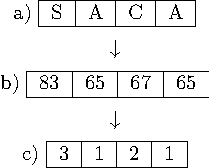
\includegraphics[scale=1]{kapitel/4_komponenten/techniken/bilder/effExample.pdf}
\caption{Beispiel für ein effektives Alphabet: a) zeigt den Eingabestring b) zeigt die entsprechenden ASCII-Werte c) zeigt die entsprechende effektive Darstellung.}
\end{figure}
Innerhalb unseres Frameworks wird das effektive Alphabet mittels des Objekts \mintinline{cpp}{alphabet} realisiert. Dieses nimmt dazu einen \mintinline{cpp}{string_span} entgegen, merkt sich welche Zeichen darin vorkommen und überschreibt schließlich die Eingabe mit den jeweiligen effektiven Werten. \\
Das Framework bestimmt für jede Eingabe automatisch das effektive Alphabet, welches dann an die Algorithmen übergeben wird. 

\subsection{Wordpacking}
\label{wordpacking}
Beim Wordpacking \cite{Manber1993} handelt es sich um eine Technik, bei der mittels Transformation der Eingabe mehrere Zeichen mit nur einer Vergleichsoperation betrachtet werden sollen. Dabei wird angenommen, dass die Alphabetgröße $|\Sigma|$ durch einen nicht-negativen Integer dargestellt werden kann.\\
Die Zeichen des Alphabets werden dann durch einen numerischen Wert $x \in \mathbb{N}$  entsprechend ihrer Wertigkeit im Intervall $[l,k]$,  mit $l,k \in \mathbb{N}$, dargestellt, wobei das Terminalsymbol $\$$ die Wertigkeit 0 hat. Im Falle eines effektiven Alphabets würde dieses Intervall also $[1,|\Sigma|]$ entsprechen. Darauf aufbauend berechnen wir den maximalen Wert für $r \in \mathbb{N}$, sodass $(|\Sigma|+1)^r$ in ein Maschinenregister passt.\\
Die Idee ist es nun den ungenutzten Platz innerhalb eines Registers zu nutzen, um dort zusätzliche Informationen über die nachfolgenden Zeichen mitzuspeichern und dabei den Stellenwert dieses Zeichens mit zu berücksichtigen. Dafür transformieren wir die Stellen des gegeben Textes $\mathsf{T}$ in den gepackten $\mathsf{T}_{packed}$ wie folgt:
\begin{equation}
\mathsf{T}_{packed}[i]= \sum_{j=1}^r x_{i+j-1}\cdot(|\Sigma|+1)^{r-j}, \text{mit }  x_i =0 \text{ für } i\geq n
\end{equation}
Dabei multiplizieren wir jede Integerrepräsentation eines Buchstabens zunächst mit $(|\Sigma|+1)^{r-1}$, dann die darauf folgende Stelle mit $(|\Sigma|+1)^{r-2}$ etc., wobei der Faktor $(|\Sigma|+1)^{r-j}$ mit einer Gewichtung vergleichbar ist. Dadurch erhalten wir für jede Stelle einen Wert, der die Wertigkeit von sich und seinen $r-1$ Nachfolgern repräsentiert. Sehen wir uns dazu ein Beispiel an:\\
Gegeben sei der String $\mathsf{T} = abac\$$ mit $|\Sigma|=3$. Die Wertigkeiten der Zeichen lassen sich wie folgt darstellen: 
\begin{center}
\begin{tabular}{c | c}
Zeichen & Wert \\
\hline
$\$$ & 0 \\
a & 1 \\
b & 2 \\
c & 3 
\end{tabular}
\end{center}

Der Einfachheit halber neben wir $r=3$ an. Daraus resultiert folgende Transformation des Textes:
\begin{flushleft}
$\mathsf{T}_{packed}[0]=$ $w(a)* 4^{2}+w(b)* 4^{1}+w(a)*4^{0}=25$\\
$\mathsf{T}_{packed}[1]=$ $w(b)* 4^{2}+w(a)* 4^{1}+w(c)*4^{0}\hspace{1pt} =39$\\
$\mathsf{T}_{packed}[2]=$ $w(a)* 4^{2}+w(c)* 4^{1}+w(\$)*4^{0}=28$\\
$\mathsf{T}_{packed}[3]=$ $w(c)* 4^{2}+w(\$)*4^{1}\hspace{52pt} =48$\\
$\mathsf{T}_{packed}[4]=$ $w(\$)* 4^{2}\hspace{103pt}=0$
\end{flushleft}
Hätten wir vor der Transformation die Stellen 0 und 2 des Textes verglichen, wäre das Resultat Gleichheit. Vergleichen wir dagegen die selben Stellen in der transformierten Eingabe, können wir anhand der zusätzlichen Informationen über die nachfolgenden Stellen sagen, dass das in 0 beginnende Suffixe lexikographisch kleiner ist als das an Stelle 2. Dadurch kann beispielsweise ein vergleichsbasierter Sortieralgorithmus mit dem selben Aufwand eine genauere Sortierung berechnen.\\
Das Wordpacking lässt sich zudem beschleunigen, indem bei der Berechnung das Ergebnis der vorherigen Stelle mit berücksichtigt wird. Für $i > 0$ lässt sich die Berechnung wie folgt umformulieren:
\begin{equation}
\mathsf{T}_{packed}[i] := (\mathsf{T}_{packed}[i-1] \% (|\Sigma|+1)^{r-1})*(|\Sigma|+1) + x_{i+r}
\end{equation}
Durch die Modulo-Operation wird der Beitrag der $(i-1)$-ten Stelle aus dem Beitrag entfernt. Dazu erhöhen wir die Wertigkeit der übrigen Stellen mit der Multiplikation und erhöhen den Beitrag zudem um den Wert des neu ins Fenster gerückten Zeichens.
Runden wir darüber hinaus $(|\Sigma|+1)$ auf die nächste Zweierpotenz auf, lassen sich die Modulo- und Multiplikationsoperatoren durch schnellere \textit{shift}- und \textit{and}- Operationen ersetzen. \\
Dieses Verfahren ist vor allem bei vergleichsbasierten Sortierern hilfreich, da mit einem Vergleich direkt $r$ Stellen berücksichtigt werden. Genutzt wird dieses beispielsweise vom qSufSort (Kapitel 5.1) oder vom Prefix Doubling Algorithmus (Kapitel 5.2).

\subsection{ISAtoSA}
\label{isa2sa}
Einige der im Framework enthaltenden Algorithmen, wie beispielsweise der mSufSort oder der qSufSort, konstruieren anstelle des eigentlichen Suffix-Arrays stattdessen die inverse Permutation, das inverse Suffix-Array. \\
\begin{definition}[Inverses Suffix-Array]
Das Inverse Suffix-Array, kurz $\mathsf{ISA}$, bezeichnet ein Array, in dem zu jedem
Suffix sein lexikographischer Rang gespeichert wird, der seiner Position
im Suffix-Array entspricht.\\
Es gilt also $\mathsf{ISA}[\mathsf{SA}[i]]=i.$
%, falls $\mathsf{ISA}$[$i$] = $j$, dann $\mathsf{SA}$[$j$] = $i$.
\end{definition}
Um daraus das $\mathsf{SA}$ konstruieren zu können, wurden innerhalb des Frameworks drei unterschiedliche Ansätze implementiert, die wir im Folgenden vorstellen werden.
\subsubsection{Simple Scan}
Wie der Titel andeutet, handelt es sich bei dieser Variante um den straight-forward Ansatz, der über die Indizes iteriert und die Einträge im $\mathsf{SA}$ wie folgt überschreibt:
\begin{equation}
\mathsf{SA}[\mathsf{ISA}[i]]=i, \text{ für } 0\leq i < n
\end{equation}

Voraussetzung für diese Methode ist, dass der Speicherplatz für sowohl das $\mathsf{SA}$, als auch das $\mathsf{ISA}$ bereits verfügbar ist. Nachteil dieser Methode ist es, dass viele zufällige Sprünge innerhalb des Suffix-Arrays gemacht werden, worunter die Cache-Effizienz leidet. 
\subsubsection{Inplace Scan}
Im Fall, dass ausschließlich Speicher für das $\mathsf{ISA}$ zur Verfügung steht, eignet sich der Simple Scan nicht, da dafür zusätzlicher Speicher für ein Array der Länge des Textes allokiert werden müsste. Daher wurde darüber hinaus eine Variante implementiert, die \textit{inplace} arbeitet, also ausschließlich das gegebene $\mathsf{ISA}$ Array nutzt und darin auch das Ergebnis speichert \cite{saca:8}. Voraussetzung dafür ist, dass die Ränge im vorliegenden $\mathsf{ISA}$ kleiner $0$ sind.\\
Die Idee ist, es zyklisch die Ränge im $\mathsf{ISA}$ durch die Positionen im $\mathsf{SA}$ zu ersetzen. Angenommen, wir finden Rang $r = \mathsf{SA}[s]$. Nun überschreiben wir $\mathsf{ISA}[r-1]=r$ merken uns aber den vorherigen Inhalt, um nach dem Überschreiben weiter dahin springen zu können. Auf diese Weise durchlaufen wir das Array bis jeder Rang durch einen $\mathsf{SA}$-Index ersetzt wurde.\\
Vorteil dieser Methode ist, wie bereits erwähnt, dass kein zusätzlicher Speicherplatz für das Ergebnisarray benötigt wird. Der allerdings weiterhin bestehende Nachteil ist, dass viele zufällige, cache-unfreundliche Sprünge gemacht werden. Zudem wird das letzte Bit zur Unterscheidung zwischen Rängen und Indizes benötigt, wodurch der Wertebereich eingeschränkt wird.
\subsubsection{Multi Scan}
Die Multi Scan Variante von Maniscalco und Puglisi \cite{saca:8} soll im Gegensatz zu den beiden vorherigen Methoden cache-freundlich arbeiten und dabei weniger zusätzlichen Speicher benötigen als die \textit{Simple Scan} Variante.\\
Wir definieren $Q_i$ mit $i \in \{1,2,3,4\}$, als $i$-tes Viertel des $\mathsf{SA}$. Zu Beginn des Algorithmus werden zwei zusätzliche Arrays $x_a$ und $x_b$ mit jeweils der Größe $\frac{n}{4}$ angelegt. In der ersten Phase wird das $\mathsf{ISA}$ von links nach rechts durchlaufen und falls ein Rang $r$ aus $Q_1$ gefunden wurde, wird dieses an die Stelle $x_a[r]$ verschoben und seine Position in $\mathsf{ISA}$ als leer markiert. Nach Abschluss der ersten Phase liegt $Q_1$ sortiert in $x_a$.\\
In der zweiten Phase scannen wir das $\mathsf{ISA}$ erneut von links nach rechts. Finden wir nun einen Rang $r \in Q_2$ speichern wir diesen an der jeweiligen Position in $x_b$ und markieren auch hier die Position in $\mathsf{ISA}$ als leer. An jede leere Position die wir während des Scans finden oder erzeugen, verschieben wir die erste besetze Position aus $x_a$ und markieren ihre Zugehörigkeit zu $Q_1$ mit Hilfe eines Bit-Tags. \\
Die dritte und vierte Phase laufen analog ab. Wir durchlaufen also das $\mathsf{ISA}$ und verschieben die jeweiligen Ränge aus $Q_i$ in das zu dem Zeitpunkt freie Hilfsarray. \\
Nach Ablauf der vierten Phase haben wir also die Ränge aus $Q_4$ in $x_b$ gespeichert und $\frac{n}{4}$ freie Stellen am Ende des $\mathsf{ISA}$ Arrays. Wir kopieren $x_b$ ans Ende von $\mathsf{ISA}$, wodurch die Elemente aus $Q_4$ dann an der richtigen Stelle stehen und nicht weiter beachtet werden müssen.\\
In der nächsten Phase müssen dann also ausschließlich die Ränge aus $Q_1,Q_2$ und $Q_3$ in die richtige Reihenfolge gebracht werden. Dazu scannen wir erneut das $\mathsf{ISA}$ Array von links nach rechts bis wir die Position $\frac{3n}{4}-1$ erreichen. Finden wir dabei ein Element aus $Q_2$, verschieben wir dieses nach $x_a$ und Elemente aus $Q_3$ nach $x_b$. Ränge aus $Q_1$ werden dabei an die erste freie Position in $\mathsf{ISA}$ verschoben. Die Zugehörigkeit eines Ranges lässt sich dabei anhand des Tags feststellen. Zum Ende des Scans haben wir dann also $Q_1$ am Anfang des $\mathsf{ISA}$, $Q_2$ in $x_a$ und $Q_3$ in $x_b$. \\
In der letzten Phase wird dann $x_a$ nach $\mathsf{ISA}[\frac{n}{4},...,\frac{n}{2}-1]$ und $x_b$ nach \\ $\mathsf{ISA}[\frac{n}{2},...,\frac{3n}{4}-1]$ verschoben. Wir erhalten also an dieser Stelle das fertige $\mathsf{SA}$ Array. EIn Beispiel für diese Variante zeigt Abb. $\ref{multiscan}$\\
Auch wenn bei dieser Variante deutlich mehr Durchläufe durch das $\mathsf{ISA}$ Array gemacht werden, behaupten die Autoren, dass dadurch das es sich dabei lediglich um cache-freundliche Scans von links nach rechts handelt, Laufzeit im Gegensatz zu den cache-unfreundlichen Varianten gewinnen zu können. Nachteile dieser Variante sind jedoch zum einen die höhere Komplexität im Vergleich zu den beiden vorherigen Varianten und zum anderen, dass hierbei die drei MSB für Tags benötigt werden, wodurch hier, noch mehr als bei der inplace Variante, der Wertebereich eingeschränkt wird.
\begin{center}
\begin{figure}
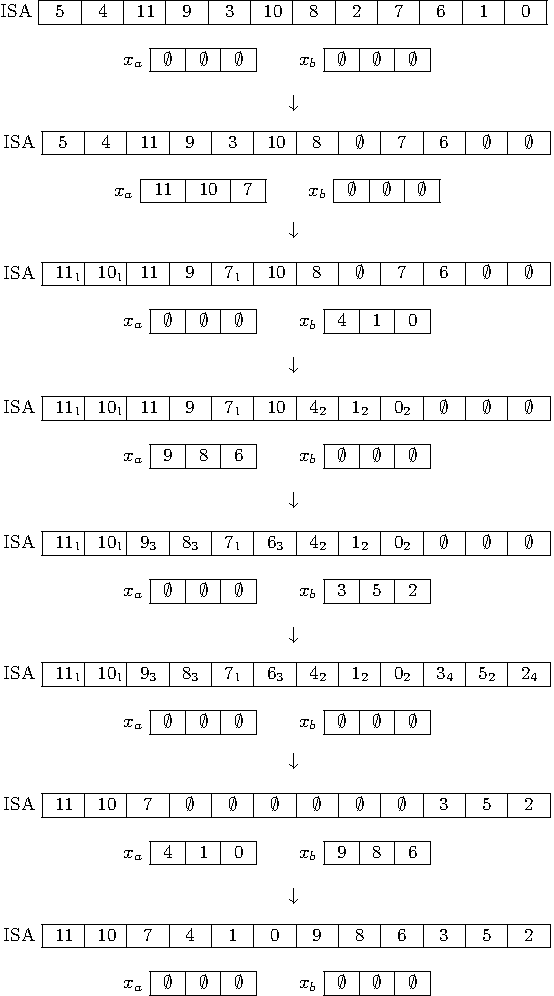
\includegraphics[scale=1]{kapitel/komponenten/techniken/bilder/MultiScanExample.pdf}
\caption{Beispiel für den ISAtoSA Multi Scan anhand des $\mathsf{ISA}$ für den Text $\mathsf{T}=MISSISSIPI\$$.}
\label{multiscan}
\end{figure}
\end{center}



\chapter{SACA Übersicht}
\section{Historie}
Alle \currentauthor{David Piper} in dieser Ausarbeitung vorgestellte Algorithmen zur Konstruktion des Suffix Arrays lassen sich in drei Gruppen einteilen, welche die grundlegenden Sortierverfahren beschreiben. \par
Die erste Gruppe bilden die sogenannten \textit{prefix doubler}, zu welcher die Algorithmen Prefix Doubling und qSufSort gehören.
Wie in Abschnitt \ref{sec:ansatz:doubler} beschrieben wird, sortieren diese die Präfixe der Suffixe und können durch geschickte Ideen die Sortierung beschleunigen, indem die Anzahl der betrachteten Präfixe in jedem Schritt verdoppelt wird. 
Dabei setzte der SACA Prefix Doubling die Grundlagen für diese Kategorie, auf der dann qSufSort aufbaute, um eine effizientere Konstruktion des Suffix Arrays zu ermöglichen. 
Neben diesen beiden Algorithmen gehört auch der Algorithmus BPR teilweise in diese Gruppe, nutzt jedoch auch Ideen eines zweiten Verfahrens, dem \textit{Induzieren}. \par

Zur Gruppe der Induzierer gehören auch die Algorithmen Deep-Shallow, DivSufSort, mSufSort, SAIS und GSACA.
Sie sortieren Suffixe anhand bereits zuvor sortierter Suffixe.
Dieses Konzept wird näher im Absatz \ref{section:induzierer} beschrieben.
Deep-Shallow war von den hier behandelten Algorithmen der erste, welcher dieses Verfahren nutzte.
Von ihm wurde der Algorithmus DivSufSort inspiriert, dessen Implementierungsdetails teilweise in die Entwicklung von SAIS eingingen.
SAIS führte Ideen ein, welche auch von GSACA aufgegriffen wurden.
Hingegen bildet mSufSort eine neu Vererbungslinie und baut auf keinem der anderen SACAs auf.
Auch nzSufSort und SACA-K gehörten zu dieser Gruppe, kombinieren das induzierte Sortieren jedoch mit dem Konzept der letzten Gruppe. \par

Diese nutzt Rekursion um kleinere Teilmengen von Zeichen zu Sortieren, welche dann zum finalen Suffix Array zusammengesetzt werden.
Zusätzlich zu nzSufSort und SACA-K wird dieses Sortierverfahren auch von den SACAs DC3, SADS und GOTO verwenden. 
Der erste Algorithmus, welcher rekursiv arbeitete um ein Suffix Array zu erstellen, war DC3. 
Zusammen mit einem anderen Algorithmus, welcher die Konzepte des induzierten Sortierens und der Rekursion kombinierte, inspirierte DC3 den Algorithmus nzSufSort. 
Dieser andere Algorithmus war ebenfalls die Grundlage für den zuvor bereits genannten SAIS sowie zusätzlich für den ähnlichen Algorithmus SADS.
SACA-K, welcher sowohl induziert als auch rekursiv arbeitet, ist eine Weiterentwicklung der Ideen von SAIS und SADS und stellt dabei sowohl eine Verbesserung der Laufzeit als auch des Speicherverbrauchs dar.
Zuletzt leitet sich GOTO direkt von SACA-K ab. \par

\begin{figure}[H]
	\centering
	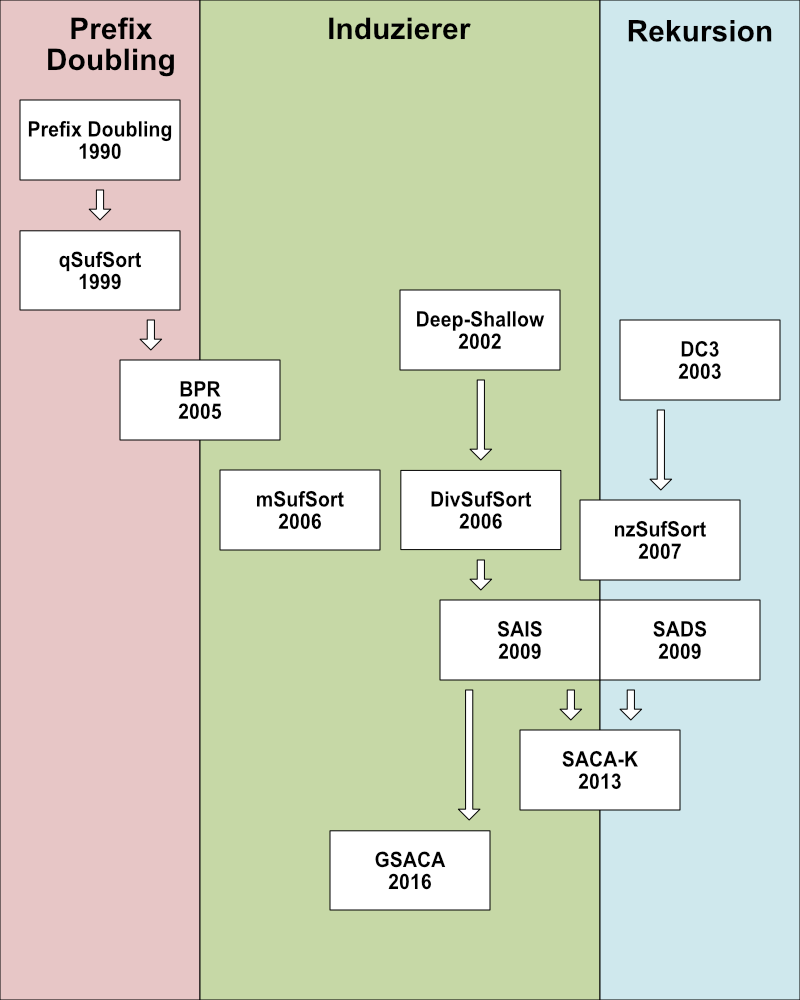
\includegraphics[width=\linewidth]{kapitel/5_saca_uebersicht/history/history3}
	\caption{Geschichtliche Entwicklung von SACAs, die in dieser Ausarbeitung betrachtet werden.}
	\label{fig_banane_1_2}
\end{figure}

\section{Ansätze}
\subsection{Doubler}
\label{sec:ansatz:doubler}
Der \currentauthor{Oliver Magiera und Marvin Löbel} erste besprochene Ansatz behandelt das Doubling, auch Prefix-Doubling genannt.
Die grundsätzliche Idee ist es, für jedes $T_i$ nur einen Präfix von $2^k$ Zeichen zu betrachten und lexikographisch zu sortieren. Falls die so betrachteten $T[i, i + 2^k)$ Strings paarweise verschieden sind, ergibt sich aus ihren Startindizen $i$ das gesuchte Suffix-Array. 

Der Prozess wird iterativ durchgeführt, und beginnt bei $k = 1$. Falls nach einer Sortierung individuelle Präfixe mehr als einmal vorkommen, sprich nicht \textit{eindeutig} sind, wird der Vorgang mit $k + 1$ wiederholt. Erst wenn alle Suffixe eindeutig sortiert sind, endet das Prefix-Doubling.

Da die Länge und Häufigkeit von gemeinsamen Prefixen somit das Laufzeitverhalten von Doubling-Algorithmen beeinflusst, definieren wir für sie relevante Kenngrößen:

$\textbf{Lcp}(i, j)$ bezeichnet die längste gemeinsamen Präfix Länge (\textbf{longest common prefix}) zwischen $\sa[i]$ und $\sa[j]$, und ist $0$ wenn $i, j \notin [0, n)$ oder die beiden Suffixe keinen gemeinsamen Präfix haben. Für jedes $\suffix i$ definieren wir $\textbf{dps}(i) = 1 + \max\{\text{lcp}(i - 1, i), \text{lcp}(i, i + 1)\}$ als charakteristische Präfixlänge (\textbf{distinguishing prefix size}). Wir definieren:
\begin{gather*}
\text{maxlcp} := \max_{i \in [0, n)} \text{lcp}(i, i + 1) 
\qquad\qquad
\log \text{dps} := \frac{1}{n} \sum_{i \in [0, n)} \log(\text{dps}(i))
\end{gather*}

Umgangssprachlich drückt maxlcp aus, welche maximale Prefixlänge das Doubling erreichen muss, während $\log \text{dps}$ die durchschnittlichen Anzahl an Doubling-Schritten ausdrückt.

Um ein Suffix-Array für $\inputtext$ zu bestimmen, müssen alle Suffixe $\suffix i$ lexikographisch sortiert werden. Wir stellen fest, dass hierfür von der Sortierfunktion jeweils nur ein Präfix von bis zu $\text{dps}(i)$ Zeichen von $\suffix i$ betrachtet werden muss.
\subsection{Sortierer}
Ein \currentauthor{Marvin Böcker} prinzipiell einfacher Ansatz um das SA zu konstruieren
ist selbstverständlich das Sortieren von Suffixen mittels einem allgemeinen Sortieralgorithmus,
wie beispielsweise Quicksort oder Radixsort.

Um einen Sortieralgorithmus zu verwenden, um das SA direkt zu konstruieren,
muss eine passende Vergleichsfunktion verwendet werden:
Nehmen wir an, die Menge die sortiert werden soll, ist bereits ein Array von disjunkten Suffixindices.
\footnote{Dies kann zu Beginn sichergestellt werden, indem das
Array mit den Zahlen von 0 bis $n-1$ (bzw $n$, wenn das Sentinel mitsortiert werden soll) gefüllt wird.}
In der Vergleichsfunktion vergleichen wir dann die Suffixe aus dem Text, die am entsprechenden Index starten.
In Abbildung 1 findet sich Pseudocode für eine simple Vergleichsfunktion,
welche die gesamten Suffixe naiv miteinander vergleicht.

\begin{figure}[!h]
\begin{minted}[mathescape=true,escapeinside=||]{python}
def compare(i, j):
    if |$\inputtext[i]$| == |$\inputtext[j]$|:
        return compare(i + 1, j + 1)
    return |$\inputtext[i]$| < |\inputtext[j]|
\end{minted}
\caption{Pseudocode einer naiven Suffixvergleichsfunktion}
\end{figure}
%
Es ist klar, dass mit einem $\mathcal O(n \log n)$-Sortieralgorithmus wie beispielsweise Merge- oder Introsort der gesamte SACA eine Worst-Case-Laufzeit von $\mathcal O(n^2 \log n)$ hat, da jeder Suffixvergleich eine Worst-Case-Laufzeit von $\mathcal O(n)$ hat.
Zum Vergleich: Es gibt einige Linearzeitalgorithmen für die SA-Konstruktion, beispielsweise DC3~\cite{saca:9} oder SAIS~\cite{saca:6}.

Die alleinige Sortierung von ganzen Suffixen ist offensichtlich nicht effizient.
Viele unserer implementierten Algorithmen verwenden allerdings zum Teil allgemeine Sortierverfahren,
um verschiedene Mengen zu sortieren: Suffixindicies, ganze Suffixe oder eine Menge von Zeichen.
Beispielsweise verwendet Multikey-Quicksort den Quicksort-Algorithmus, um eine Menge von Zeichen zu sortieren.
Deep-Shallow verwendet Introsort, um die Suffixe nach ihrer Länge zu sortieren
und DC3 benutzt Radixsort um Triplets zu sortieren.
In DivSufSort werden Stringsortierer benutzt, um bestimmte Substrings zu sortieren.
Daher ist es für unsere Bibliothek wichtig, auch diese allgemeinen Sortierverfahren angepasst
auf unseren Use-Case effizient zu implementieren.
In Abschnitt \ref{section:sortieralgorithmen} findet sich eine Übersicht über die von uns
implementierten Sortieralgorithmen.


\subsection{Induzierer}
\label{section:induzierer}
Das \currentauthor{Jonas Bode} Prinzip des \textit{Induced Sortings} (zu deutsch \textit{induziertes Sortieren}) baut darauf auf, dass das gesamte Suffixarray aus mehreren einzelnen sortierten Komponenten zusammen gesetzt werden kann. Diese Komponenten entstehen aus den Suffixen des Eingabestrings und hängen maßgeblich von dem ersten Symbol der zugehörigen Suffixe ab. Die Idee des Induced Sortings ist es, zuerst für jedes im String vorkommenden Symbol $\sigma$ alle Suffixe des Eingabestrings, welche mit $\sigma$ beginnen, in den $\sigma$-\textit{Bucket} ein zu ordnen. Sind für jedes im Text vorkommende Symbol alle Suffixe in ihren Buckets korrekt geordnet, so können die Buckets aneinander gereiht werden, vorgegeben durch die Ordnung der Symbole selber, um das vollständige SA zu erhalten. \\

Es folgt ein Beispiel einer Zerteilung eines $\mathsf{SA}$ in die Buckets der jeweiligen Symbole, anhand des Textes $\inputtext = abracadabra\$$, mit dem dazugehörigen Suffixarray $\mathsf{SA}(\inputtext) = [11, 10, 7, 0, 3, 5, 8, 1, 4, 6, 9, 2]$. Dieses lässt sich wie folgt unterteilen:

\begin{center}
\begin{tabular}{c}
$\mathsf{SA}(\inputtext) = \underbrace{[11]}_{\$} \cdot \underbrace{[10,7,0,3,5]}_{a} \cdot \underbrace{[8,1]}_{b} \cdot \underbrace{[4]}_{c} \cdot \underbrace{[6]}_{d} \cdot \underbrace{[9,2]}_{r}$ \\
\end{tabular}
\end{center}

Bei dieser Unterteilung fällt sofort auf, dass der Sentinel \$ immer einen eigenen Bucket mit nur einem Eintrag zugeteilt bekommt, welcher immer am Anfang des SAs steht. Das Alphabet eines Strings $\inputtext$ wird hier in den meisten Fällen mit $\Sigma(\inputtext)$ angegeben und beinhaltet nicht den Sentinel.  \\
Die gängigen Induzierer unterteilen jeden Bucket in zwei Sub-Buckets, in denen die Suffixe nach dem Kriterium eingeordnet werden, ob ihr zweites Symbol größer oder kleiner als ihr erste Symbol ist. Wir führen daher die folgende Notation ein für ein Suffix $\mathsf{S}_i$ (bzw. analog für die Stelle $\inputtext[i]$):

\begin{itemize}
\item Wir sagen $\mathsf{S}_i$ ist ein \textit{S-Typ}, falls $\inputtext[i] < \inputtext{}[i+1]$ oder $\inputtext[i] = \$$ gilt.
\item Wir sagen $\mathsf{S}_i$ ist ein \textit{L-Typ}, falls $\inputtext[i] > \inputtext{}[i+1]$ gilt.
\item Weiterhin haben $\mathsf{S}_i$ und $\mathsf{S}_{i+1}$ den selben Typ, falls $\inputtext[i] = \inputtext[i+1]$ gilt.
\item Wir sagen $\mathsf{S}_i$ für $i > 0$ ist ein \textit{LMS-Suffix} (Leftmost-S-Type-Suffix), falls $\mathsf{S}_i$ ein S-Typ ist und $\mathsf{S}_{i-1}$ ein L-Typ ist.
\item Wir sagen $\inputtext{}[i,j]$ ist ein \textit{LMS-Substring}, falls $\mathsf{S}_i$ und $\mathsf{S}_j$ LMS-Suffixe sind oder $\inputtext{}[i,j] = \$$ gilt.
\item Wir sagen $\mathsf{S}_i$ für $i > 0$ ist ein \textit{RMS-Suffix} (Rightmost-S-Type-Suffix), falls $\mathsf{S}_i$ ein S-Typ ist und $\mathsf{S}_{i+1}$ ein L-Typ ist.
\item Wir sagen es gilt Type($\mathsf{S}_i$) = S, falls $\mathsf{S}_i$ ein S-Typ ist (analog für L-Typen).
\end{itemize}

Analog wird das Suffix $\mathsf{S}_i$ in diesem Kontext auch als suf$(\inputtext,i)$ bezeichnet, wenn klar gemacht wird, um welchen String $T$ es sich handelt. Diese Unterscheidung kann bei Induzierern sehr wichtig sein, da sie für ihre Rekursionsinstanzen neue Strings erzeugen.

Induzierer unterteilen jeden Bucket nun in einen L- und einen S-Bucket. Dabei befinden sich in den L-Buckets alle Suffixe welche ein L-Typ sind -- analog für S-Buckets. Für alle Indizes $i,j$ mit $\inputtext{}[i] = \inputtext{}[j]$, so dass $\mathsf{S}_i$ ein L-Typ und $\mathsf{S}_j$ ein S-Typ ist, gilt, dass $i$ vor $j$ in $\mathsf{SA}$ vorkommt. Intuitiv formuliert kommt ein L-Bucket für das Symbol $\sigma$ also immer vor dem S-Bucket von $\sigma$, da die Suffixe im L-Bucket ein niedrigeres zweites Symbol enthalten als die Suffixe im S-Bucket. \\
Dazu betrachten wir das Beispiel von oben, mit dem Text $\inputtext = abracadabra\$$ und dem dazugehörigen Suffixarray $\mathsf{SA}(\inputtext) = [11, 10, 7, 0, 3, 5, 8, 1, 4, 6, 9, 2]$. Der $a$-Bucket besteht aus den Einträgen $[10,7,0,3,5]$, wie wir oben bereits gesehen haben, setzt sich aber aus dem L-Bucket $[10]$ und dem S-Bucket $[7,0,3,5]$ zusammen, da das Suffix $\inputtext{}[10,12) = a\$$ ein L-Typ ist, und alle anderen Suffixe S-Typen sind. \\
Oft wird das erste Element eines Buckets als \textit{start} und das letzte Element eines Buckets als \textit{end} bezeichnet. \\

Eine weitere gemeinsame Eigenschaft der Induzierer ist das Konzept, nach dem sie die Buckets jedes Suffixes ordnen. Sie ordnen dazu zuerst die LMS-Substrings in ihre jeweiligen Buckets ein. Wird dann erkannt, dass es zwei identische LMS-Substrings gibt, welche natürlich voneinander verschiedene LMS-Suffixe haben müssen, so werden diese mittels eines Rekursionsaufrufes und einer Umbenennung abhängig von ihren Positionen neu geordnet, so dass sich am Ende der Rekursion eine korrekte Ordnung der LMS-Substrings ergibt aus der sich auch die Ordnung der LMS-Suffixe herleiten lässt. \\
Im Folgenden wird erklärt, wie aus der korrekten Ordnung der LMS-Substrings bzw. der LMS-Suffixe das gesamte SA induziert werden kann:
\begin{itemize}
\item \textbf{Einordnung der LMS-Typen in $\mathsf{SA}$}: Der Eingabestring wird von rechts nach links durchgelaufen und jeder LMS-Typ wird so weit rechts wie möglich in dem ihm zugehörigen S-Bucket platziert.
\item \textbf{Erste Iterationsphase}: $\mathsf{SA}$ wird von links nach rechts durchgelaufen und von jedem Eintrag $i$ wird das Suffix an der Stelle $i-1$ überprüft. Ist dieses ein L-Typ, so wird es in den Bucket passend links eingeordnet.
\item \textbf{Zweite Iterationsphase}: $\mathsf{SA}$ wird von rechts nach links durchgelaufen und von jedem Eintrag $i$ wird das Suffix an der Stelle $i+1$ überprüft. Ist dieses ein S-Typ, so wird es in den Bucket passend rechts eingeordnet.
\end{itemize}

Es gibt dabei viele verschiedene Implementierungen dieses Vorgangs, welche von Algorithmus zu Algorithmus unterschiedlich sein können. Die größten Unterschiede dabei liegen hauptsächlich bei der Berechnung der Typen, welche entweder dynamisch berechnet werden können oder am Anfang berechnet und dann für spätere Aufrufe gespeichert werden können. Es lässt sich zeigen:

\begin{lemma}[Gemeinsamer Präfix]
	\label{lemma:common_prefix}
	\normalfont
    Haben zwei Suffixe \suffix{i} und \suffix{j} einen gemeinsamen Präfix der Länge {\textit{offset}\xspace}, so ist \(\suffix{i} \leq \suffix{j}\) genau dann, wenn \(\suffix{i+{\textit{offset}\xspace}} \leq \suffix{j+{\textit{offset}\xspace}}\). Dies folgt direkt aus der Definition der lexikographischen Ordnung.
\end{lemma}


\chapter{Suffix-Array-Konstruktionsalgorithmen}
\section{qSufSort}

\newtheorem{lemma}{Lemma}
In diesem Abschnitt wird der von Larson und Sadakane entworfene Algorithmus qSufSort \cite{saca:1} vorgestellt. 
Dieser garantiert für die Konstruktion des Suffix-Arrays eine Laufzeitschranke von $\mathcal{O}(n\log n)$ und benötigt dafür ausschließlich zwei Integerarrays der Länge $n$.

Dabei werden wir uns zunächst im folgenden Abschnitt mit der allgemeinen Funktionsweise des Algorithmus auseinander setzen. Anschließend werden die von den Autoren vorgestellten praktischen Verbesserungen präsentiert. In Kapitel \ref{qsufsort:example} folgt dann ein Beispiel zur Durchführung des qSufSort. Schließlich werden wir Details zur Implementierung des Algorithmus innerhalb unseres Frameworks präsentieren.

\subsection{Algorithmus}
\label{qsufsort:algo}
Grundgedanke des Algorithmus ist, dass die Suffixe eines Suffix die Präfixe der darauf im String folgenden Suffixe sind und diese bereits in einem anderen Bereich des Suffix-Arrays teils sortiert vorliegen. Anstatt also erneut Zeichen zu vergleichen, die wir bereits verglichen haben, nutzen wir vorhandene Teilresultate.
Wichtig ist hierbei die Rolle der sogenannten $h$-Reihenfolge:
\begin{definition}[$h$-Reihenfolge]
Gegeben seien die Suffixe $\mathsf{S}_i$ eines Strings $\mathsf{T}$ mit $i \in \{0,...,n\}$. Die Suffixe liegen in \textit{h-Reihenfolge} vor, falls die Reihenfolge der lexikographischen Sortierung ausschließlich auf den ersten $h$ Zeichen eines Strings beruht. 
\end{definition}
Eine Sortierung nach ausschließlich dem Anfangszeichen eines Strings, würde demnach eine 1-Reihenfolge ergeben. Zudem muss eine $h$-Reihenfolge nicht zwingend eindeutig sein. Beispielsweise sind die Positionen der Strings $aab$, $aaa$ und $aaab$ innerhalb einer 2-Reihenfolge untereinander nicht eindeutig. 

Bezüglich der $h$-Reihenfolge lässt sich zudem der Begriff der Gruppe definieren:
\begin{definition}[Gruppe]
Sei $\sa$ ein Suffix-Array in $h$-Reihenfolge. Eine Sequenz aufeinander folgender Suffixe in $\sa$, dessen ersten $h$ Zeichen übereinstimmen, wird als \textit{Gruppe} bezeichnet. Befindet sich innerhalb einer Gruppe nur ein Suffix, handelt es sich um eine \textit{sortierte} Gruppe, andernfalls um eine \textit{unsortierte} Gruppe. 
Eine Sequenz von sortierten Gruppen wird \textit{kombinierte sortierte} Gruppe genannt.
\end{definition}

\subsubsection{Logarithmische Schranke für Vergleiche}
Grund dafür, dass der straight-forward Ansatz mittels direkter Vergleiche ähnlich wie bei der Sortierung von Zahlen nicht effizient genug arbeitet, ist, dass für den Vergleich zweier Suffixe die Anzahl der direkten Zeichenvergleiche linear in der Länge des Strings ist. Wünschenswert wäre es daher zwar ähnlich viele Vergleiche von Stellen, aber deutlich weniger Zeichenvergleiche durchführen zu müssen.

Ein Ansatz, um die Anzahl letzterer reduzieren zu können, wurde von Karp, Miller und Rosenberg \cite{Karp} veröffentlicht und basiert auf der $h$-Reihenfolge. Folgendes Lemma von Manbers und Myers \cite{Manber1993} ist dabei essentiell:
\begin{lemma}[Manbers und Myers]
\label{manmyers}
Werden die Suffixe $\mathsf{S}_i$ zunächst nach ihrer Position in $\sa$ in der $h$-Reihenfolge und anschließend nach der Position des Suffixes $\mathsf{S}_{i+h}$ sortiert , erhalten wir die 2h-Reihenfolge.
\end{lemma}
Aufbauend darauf, können wir also zunächst die 1-Reihenfolge vergleichsbasiert berechnen, indem wir nur anhand des ersten Zeichens sortieren und uns anschließend an den bereits teilweise sortierten Suffixen der Suffixe an i+$2^j-1$-ter Stelle orientieren, wobei $j \geq 1$ der Anzahl der Durchläufe entspricht.

Hierzu zur Veranschaulichung der Idee ein kleines Beispiel:

Betrachten wir den String $\mathsf{T} =  babc\$ $. Ein Suffix-Array in 1-Reihenfolge wäre $\sa=[4,1,2,0,3]$ (alternativ auch $\sa=[4,1,0,2,3]$, da das $\sa$ nach initialer Sortierung nicht eindeutig ist). Um jetzt beispielsweise die beiden mit $ b $ beginnenden Suffixe zu sortieren, können wir uns die Position des bei jeweils $h$ beginnenden Suffixes im Array anschauen. Im Fall für $ bc\$ $  ist $\sa[\mathsf{T}[2+1]]=4$ und für $ babc\$ $ $\sa[\mathsf{T}[0+1]]=1$. Das heißt, die Suffixe, die in beiden Fällen auf das $ b $ folgen, sind bereits soweit lexikographisch im Suffix-Array sortiert, dass sich daraus eine Reihenfolge für die beiden Suffixe ablesen lässt und keine weiteren Vergleiche notwendig sind. Daraus resultiert $\sa=[4,1,0,2,3]$ und somit das fertig sortierte Suffix-Array.

Dadurch dass wir $h$ in jedem Schritt verdoppeln, reduziert sich unsere obere Schranke für die Anzahl der Vergleiche auf $\mathcal{O}(n\log n)$.
 \subsubsection{Vorgehen}
Aufbauend auf den Resultaten aus dem vorherigen Abschnitt und dem des Ternary Quicksort (s. \ref{section:ternary_quicksort}), lässt sich nun der qSufSort Algorithmus wie folgt konstruieren.
Benötigt werden neben dem Ergebnisarray $\sa$ zunächst zwei Hilfsarrays $\mathsf{V}$ und $\mathsf{L}$ der Länge $n$+1.

Array $\mathsf{V}$ speichert für das Suffix-Array $\sa$ die Nummern der Gruppen. Die Nummer einer Gruppe ergibt sich aus dem maximalen Index im Suffix-Array, den diese Gruppe belegt. Eine Gruppe, die also die Positionen $l$ bis $k$ mit $l \leq k$ in $\sa$ belegt, hat demnach die Gruppennummer $\mathsf{V}[l]=\mathsf{V}[l+1]=...=\mathsf{V}[k]=k$.

Das Hilfsarray $\mathsf{L}$ dagegen speichert die dazu gehörigen Gruppenlängen. Um kombinierte sortierte Gruppen von unsortierten besser unterscheiden zu können, wird die Länge erst als negative Länge gespeichert. Für beliebige Gruppengrenzen $l$ und $k$ mit $l \leq k$ in $\sa$ ist also die Gruppenlänge, falls unsortiert, $\mathsf{L}[l]$=($k-l+1$), anderenfalls $\mathsf{L}[l]$=$-$($k-l+1$). 

Der Algorithmus geht wie folgt vor:


\begin{listing}
\begin{minted}[escapeinside=||,mathescape=true,numbers=left]{python}
def qSufSort(T)
  Sort suffixes |$\mathsf{S}_i$| according to their first character into |$\sa$|  
  Init additional arrays |$\mathsf{V}$| |and| |$\mathsf{L}$|
  h := 1
  while (-|$\mathsf{L}$|[0] != n):
     Sort suffixes |$\mathsf{S}_i$| |in| unsorted groups |in| |$\sa$| by |$\mathsf{V}[i+h]$| 
     Mark borders of |$A_{left}$, $A_{middle}$| |and| |$A_{right}$|
     Calculate new groups 
     Update |$\mathsf{V}$| |and| |$\mathsf{L}$|
     h = h |$\cdot$| 2
\end{minted}
\caption{Pseudocode zum qSufSort}
\end{listing}
% Sortiere Suffixe |$\mathsf{S_i}$| anhand des ersten Zeichens in |$\sa$| ein 
 %Berechne |$\mathsf{V}$| und |$\mathsf{L}$|
 %|$h$ = 1|
% Do  
 %  Sortiere jede unsortierte Gruppe in |$\sa$| mit Hilfe
  %   des Ternary Quicksort mit |$\mathsf{V}[i+h]$| als Key,
   %  wobei |$i$| dem Index des Suffixes entspricht
   %Markiere dabei die Grenzen von |$A_{left}$, $A_{middle}$| und |$A_{right}$|
  % Erstelle neue Gruppen mit Hilfe der Grenzen
  % Aktualisiere |$\mathsf{V}$| und |$\mathsf{L}$|
   %|$h=2*h$|
 % Until(|$\sa$| besteht aus einer kombinierten sortierten Gruppe)


In der ersten Zeile sortieren wir zunächst die Suffixe anhand ihres ersten Zeichens in das $\sa$ ein, wodurch dieses dann in 1-Reihenfolge vorliegt. Aufbauend darauf berechnen wir dann initial die Hilfsarrays $\mathsf{L}$ und $\mathsf{V}$ und setzen die Variable $h$ auf unsere derzeitige $h$-Reihenfolge, also 1.
Die nachfolgende Schleife wiederholen wir dann solange, bis unser Suffix-Array nur noch eine kombinierte sortierte Gruppe beinhaltet, also vollständig sortiert ist und somit die Länge der ersten sortierten Gruppe der Länge des Arrays entspricht.
In dieser sortieren wir dann die einzelnen sortierten Gruppen, deren Startposition und Länge wir schnell mit $\mathsf{V}$ und $\mathsf{L}$ bestimmen können mit Hilfe des Ternary Quicksort auf Basis der Suffix-Array-Position des an $i+h$ startenden Suffixes. Die aus dem Ternary Quicksort resultierenden Partitionen $A_{left}$, $A_{middle}$ und $A_{right}$ werden entsprechend markiert. Damit versetzen wir das Ergebnisarray $\sa$ nach Lemma \ref{manmyers} in $2h$-Reihenfolge. Dementsprechend setzen wir dann $h$ auf seinen doppelten Wert, nachdem wir in Zeile 8 und 9 die Informationen zu den Gruppen in $\mathsf{L}$ und $\mathsf{V}$ mit Hilfe der Split-Positionen des Quicksorts aktualisiert haben.

\subsubsection{Laufzeit}
Die initiale Sortierung in Schritt 1 kann in $\mathcal{O}(n\log n)$ Zeit durchgeführt werden, beispielsweise mit Hilfe des Quicksort-Algorithmus. Die Berechnung der Arrays $\mathsf{V}$ und $\mathsf{L}$ ist in linearer Zeit mittels eines Scans über das Array $\sa$ möglich, sowohl in den Zeilen 2 und 3 als auch in Zeile 8. Der für die Laufzeit ausschlaggebende Teil ist die in Zeile 4 beginnende Schleife. Wie wir bereits gesehen haben, rufen wir diese höchstens $\mathcal{O}(\log n)$ mal auf. Zwar rufen wir in jedem Durchlauf in Zeile 5 den Quicksort auf, woraus sich intuitiv eine Worst-Case Laufzeit $\mathcal{O}(n\log  n)\cdot \mathcal{O}(\log n)$ = $\mathcal{O}(n(\log n)^2)$ ergeben würde, jedoch können wir diese mittels einer genaueren Analyse deutlich schärfer wählen:

Als Sortierverfahren wurde sowohl in Zeile 1 als auch in Zeile 5 der Ternary Quicksort gewählt. Der Verlauf der Partitionierungen lässt sich implizit durch einen ternären Baum darstellen (siehe Abb. $\ref{terTree}$).

Die Partitionierung eines Arrays $A$ mit $|A|=n$ lässt sich in $\mathcal{O}(n)$ berechnen. Da für die drei resultierenden Arrays $A_{left}$, $A_{middle}$ und $A_{right}$ gilt, dass diese in Summe höchstens genauso lang sind wie $A$, also $n$, können wir auch die Partitionierung der gesamten unter $A$ liegenden Ebene in $\mathcal{O}(n)$ berechnen. Daraus folgt folgendes Lemma:
\begin{lemma}
Die Partitionierung der auf einer beliebigen Ebene im ternären Baum befindlichen Teilmengen lässt sich in $\mathcal{O}(n)$ erzeugen. 
\end{lemma}
Es bleibt zu zeigen, wie hoch der ternäre Baum sein kann. Für den Pfad entlang der $A_{middle}$-Partitionen gilt, dass die Anzahl betrachteter Zeichen sich mit jeder Ebene verdoppelt. Damit ist die maximale Pfadlänge von der Wurzel zum Blatt entlang der $A_k$ Mengen kleiner gleich $ \log (n+1)$.

Für die Teilmengen $A_{left}$ und $A_{right}$ gilt, dass die Mengen in den jeweiligen Kindern höchstens halb so groß sind, da wir am Median teilen. Daraus folgt, dass auch entlang eines Pfades höchstens $\log (n+1)$ linke oder rechte Teilarrays sein können.

Daraus resultiert folgendes Lemma:
\begin{lemma}
Die Höhe eines auf diese Weise erstellten ternären Baumes ist durch $\mathcal{O}(\log n)$ beschränkt.
\end{lemma}
Fassen wir nun beide Lemmas inklusive unserer vorangegangen Überlegungen bezüglich der anderen Zeilen zusammen: 
\begin{lemma}
Die Berechnung des Suffix Arrays mit Hilfe des qSufSort-\newline Algorithmus ist in $\mathcal{O}(n\log n)$ Zeit möglich.
\end{lemma}
\begin{figure}[t]
\centering
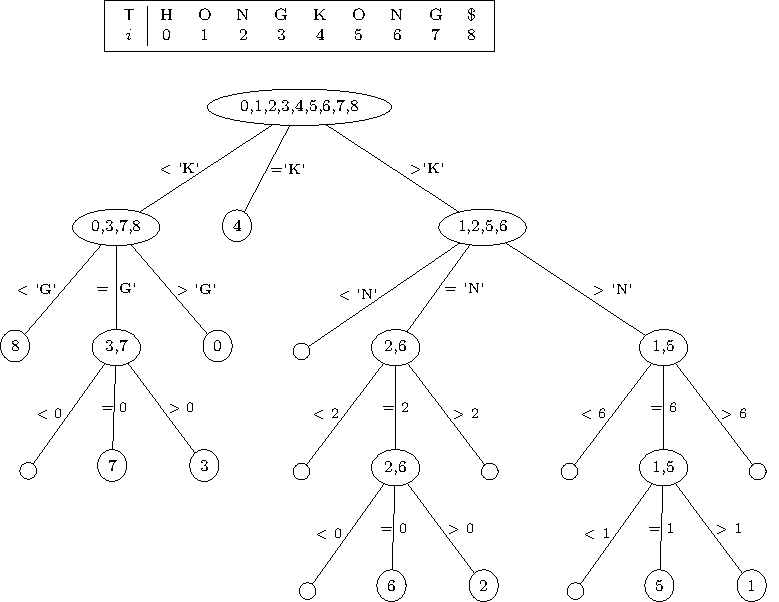
\includegraphics[scale=0.9]{kapitel/saca_algorithmen/qsufsort/Bilder/TerTree.pdf}
\caption{Der durch die ternäre Sortierung entstehende ternäre Baum anhand des Strings $\mathsf{T}=HONGKONG\$$.}
\label{terTree}
\end{figure}
\subsection{Verbesserungen}
\subsubsection{Reduzierung auf ein Hilfsarray}
Der Sinn und Zweck des Arrays $\mathsf{L}$ ist es vor dem tatsächlichen Aufruf des ternary Quicksorts innerhalb der Schleife bereits sortierte kombinierte Gruppen in konstanter Zeit überspringen und zudem die Grenzen der unsortierten Gruppen für genau diesen Aufruf setzen zu können. Letzteres lässt sich allerdings implizit über über die Gruppennummern des $\mathsf{V}$ Arrays lösen. Können wir also zudem einen alternativen Speicherort für die Längen der kombinierten sortierten Gruppen finden, können wir uns das Hilfsarray $\mathsf{L}$ sparen.

Was bei den Bereichen der kombinierten sortierten Gruppen auffällt ist, dass der korrespondierende Bereich im Ergebnisarray $\mathsf{SA}$ nicht mehr verändert wird, da sich die sortierten Gruppen laut Definition bereits an der richtigen Stelle in $\mathsf{SA}$ befinden. Daher können wir genau diesen Bereich nutzen um dort die Länge der kombinierten sortierten Gruppen zu lagern.

Das Problem, das dabei entsteht, ist, dass wir, wenn der Algorithmus terminiert, keine gültige Lösung in Array $\mathsf{SA}$ gespeichert haben, da diese überschrieben wurde. Jedoch können wir die Lösung mit Hilfe des Hilfsarrays $\mathsf{V}$ rekonstruieren, da es sich dabei um das inverse Suffix-Array handelt. Mit einer der in Kapitel \ref{isa2sa} vorgestellten Techniken lässt sich dieses nach Abschluss der Berechnung in das eigentliche Suffix-Array transformieren.



% Um also das Suffix-Array aus $\mathsf{V}$ berechnen zu können, setzen wir lediglich nach Terminierung des Algorithmus $SA[V[i]]=i$ und erhalten dadurch unser Ergebnisarray, im Folgendem anhand des Beispiels aus 3.3 gezeigt:\\
%\begin{center}
%\begin{tabular}{| c | c  c  c  c  c  c  c  c  c |}
%\hline
%$X$&H&O&N&G&K&O&N&G&\$ \\
%$i$&0&1&2&3&4&5&6&7&8 \\
%\hline
%$\mathsf{V}[i]$&3&8&6&2&4&7&5&1&0 \\
%\hline
%$SA[i]$&8&7&3&0&4&6&2&5&1 \\
%\hline
%\end{tabular}
%\end{center}
%\vspace{4pt}
Um diese jetzt noch während der Berechnung unterscheiden zu können, ob es sich bei einem Eintrag in $\mathsf{SA}$ um die bisherige Position eines unsortierten Elements oder um die Länge einer kombinierten sortierten Gruppe handelt, negieren wir wie zuvor auch schon letzteres.\\
Da wir nun also alternative Wege haben, um an die Informationen aus $\mathsf{L}$ zu kommen und diese im Falle von kombinierten sortierten Gruppen speichern können, können wir uns dieses sparen. Dies hat in erster Linie positive Auswirkungen auf den Speicherverbrauch. Dadurch, dass wir bereits allokierten Speicher in Form der Bereiche in $\mathsf{SA}$ verwenden, können wir unseren Speicherverbrauch von drei Arrays der Länge $n+1$ auf lediglich zwei reduzieren. Die benötigten Rechenoperationen erhöhen sich dagegen. Zum einen dadurch, dass das Ermitteln der Länge unsortierter Gruppen mehr Zugriffe als vorher benötigt, zum anderen durch die benötigte Invertierung des $\mathsf{V}$ Arrays um das Suffix-Array rekonstruieren zu können. Für eine verbesserte Laufzeit spricht allerdings, dass dadurch, das wir lediglich auf zwei Arrays arbeiten, unsere Implementierung womöglich cache-freundlicher arbeitet.
\subsubsection{Sortieren und Updaten kombinieren}
Ausgehend davon, dass wir noch das Hilfsarray $\mathsf{L}$ mitführen, berechnen wir dieses und das Hilfsarray $\mathsf{V}$ nach jedem Sortieraufruf separat mittels Durchlaufs durch das bisherige $\mathsf{SA}$. Ziel ist es, diese Aktualisierungen schon bereits während der Sortierung durchführen zu können, um sich weitere Durchläufe durch die Arrays sparen zu können. 

Zunächst können wir feststellen, dass das Aktualisieren der maximalen kombinierten sortierten Gruppen zum Beginn des nachfolgenden Sortieraufrufs verschoben werden kann.  

Um darauf aufbauend die gesamte Aktualisierung in die Sortierung übernehmen zu können, gehen wir wie folgt vor:
\begin{enumerate}
\item Teile das Array $A$ wie gewohnt nach dem Pivotelement in $A_{left}$, $A_{middle}$ und $A_{right}$ auf
\item Sortiere $A_{left}$ rekursiv
\item Aktualisiere die Gruppennummern und -längen der Elemente in $A_{middle}$
\item Sortiere $A_{right}$ rekursiv
\end{enumerate}

Aktualisieren wir zuerst den \glqq Gleich\grqq{}- oder \glqq Größer\grqq{}-Teil, kann es passieren, dass 
ein Suffix eine niedrigere Gruppennummer zugewiesen bekommt als ein anderes Suffix vor ihm in SA, da 
Gruppennummern lediglich kleiner werden können. Da diese als Keys für die Sortierung dienen, hätten wir dabei einen ungültigen Zustand. Daher fangen wir zunächst beim \glqq Kleiner\grqq{}-Teil an. \\

%Dadurch, dass bei der Aktualisierung von $\mathsf{V}$ die neuen Gruppennummern lediglich kleiner werden können, kann es sein, dass falls wir zuerst den \glqq Gleich\grqq{}- oder \glqq Größer\grqq{}-Teil updaten, es dazu kommen kann, dass ein Suffix eine niedrigere Gruppennummer zugewiesen bekommt als ein anderes Suffix vor ihm in SA. Da diese als Keys für die Sortierung dienen, hätten wir dabei einen ungültigen Zustand. Daher fangen wir zunächst beim \glqq Kleiner\grqq{}-Teil an. \\
Dies beeinflusst dennoch den Sortierprozess. Ohne diese Überlegung kann es nämlich sein, dass wir innerhalb der Sortierung für zwei Suffixe den selben Key haben, diese also unsortiert bleiben und damit in der nächsten Iteration wieder aufgerufen werden, obwohl die betroffenen Stellen in der selben Iteration schon soweit verarbeitet wurden, dass eine Sortierung möglich gewesen wäre. Es würde also lediglich an der Propagierung der Ergebnisse scheitern, was mit Hilfe dieser Verbesserung für dann Fall, in welchem die betroffenen Keys schon vorher abgearbeitet worden sind, nicht passieren kann. Dadurch kann es in einigen Fällen zu Einsparungen von Sortieraufrufen kommen und dadurch zu einer Verbesserung der tatsächlichen Laufzeit.
%\subsubsection{Eingabetransformation}
%Für die folgende Verbesserung qsufsort nehmen wir an, dass unser $\sigma$ klein genug ist, sodass jedes $s \in \Sigma$ mit Hilfe eines nicht-negativen Integers dargestellt werden kann.\\
%Wir definieren uns hierfür einen Zahlenbereich [$\mathsf{L},k$) wobei $k-l$= $\sigma$, beispielsweise [1,$\sigma$). Initial transformieren wir den String $X$ in das Array $\mathsf{V}$ mit $\mathsf{V}[i]=x_i - l +1$ für $i \in [0,n)$. Für das Sentinel legen wir in $\mathsf{V}[n]$ dann eine Null an. Sei zudem $r$ die größtmögliche Ganzzahl, sodass $(\sigma+1)^r-1$ in ein Maschinenwort passt, also im Fall von 64-Bit Maschinen $\leq 2^{63}$. Aufbauend darauf, definieren wir die Einträge in $\mathsf{V}$ erneut durch:
%\begin{equation}
%V[i]= \sum_{j=1}^r x_{i+j-1}*(\sigma+1)^{r-j}, \text{mit }  x_i =0 \text{ für } i\geq n
%\end{equation}
%Dabei multiplizieren wir jede Integerrepräsentation eines Buchstabens zunächst mit $(\sigma+1)^{r-1}$, dann die darauf folgende Stelle mit $(\sigma+1)^{r-2}$ etc., wobei der Faktor $(\sigma+1)^{r-j}$ damit mit einer Gewichtung vergleichbar ist. Dadurch erhalten wir für jede Stelle einen Wert, der die Wertigkeit von sich und seinen $r-1$ Nachfolgern repräsentiert. Mit Hilfe dieser Werte lässt sich nun eine initiale Sortierung konstruieren, welche anders als zuvor nicht nur ein Zeichen, sondern gleich $r$ Zeichen auf einmal berücksichtigt. Wir erhalten also eine $r$-Reihenfolge.\\
%Alternativ kann die in (1) gezeigte Transformation für $i > 0$ auch wie folgt berechnen werden:\\
%\begin{equation}
%V[i+1] := (V[i] \% (\sigma+1)^{r-1})*(\sigma+1) + x_{i+r}
%\end{equation}
%Dadurch sparen wir uns die rechenaufwendige Summe und können falls wir statt $(\sigma+1)$ die nächste Zweierpotenz nehmen, die Modulo- und Multiplikationsoperatoren durch schnellere $and$ und $shift$ Operationen ersetzen.  
\subsubsection{Initiales Sortierverfahren}
Bislang wurde nicht konkret festgelegt, welcher Sortieralgorithmus für die initiale Sortierung in Zeile 1 verwendet werden soll. Zwar wurde für die Analyse ein ternary Quicksort angenommen um mit Hilfe des ternären Baums eine möglichst scharfe Laufzeitschranke bestimmen zu können, dennoch können wir an dieser Stelle einen alternativen Algorithmus wählen, der womöglich effizienter arbeitet.

Eine Möglichkeit hierfür ist der Bucketsort-Algorithmus, welcher in linearer Zeit sortiert. Ist dabei $|\Sigma| \leq n+1$, kann die Bucket-Sortierung direkt in $\mathsf{SA}$ stattfinden. Anderenfalls ist der Algorithmus hierbei ungeeignet.

Betrachten wir dabei zusätzlich die in Kapitel \ref{wordpacking} vorgestellte Transformation der Eingabe mittels Wordpacking, können wir die Sortierung zusätzlich beschleunigen. Hierbei wird jedoch bei der Wahl von $r$ vorausgesetzt, dass nicht nur $(|\Sigma| + 1)^r$ in ein Maschinenwort passt, sondern auch, dass $r \leq  n$ gilt. Das daraus resultierende, neue Alphabet $|\Sigma|'$ kann zwar für einige Eingaben größer ausfallen als vorher, dennoch können wir durch die Bedingungen garantieren, dass die dazu gehörige transformierte Eingabe innerhalb des $\mathsf{SA}$ sortiert werden kann, ohne zusätzlichen Speicher allokieren zu müssen. Dadurch können wir, wie bereits in 4.3 gesehen, eine initiale Sortierung durchführen, die das Suffix-Array in linearer Zeit in $r$-Reihenfolge bringt.
\usetikzlibrary{decorations.pathreplacing,calc}

\newcommand{\tikzmark}[2][-3pt]{\tikz[remember picture, overlay, baseline=-0.5ex]\node[#1](#2){};}

\newcounter{arrow}
\setcounter{arrow}{0}
\newcommand{\drawcurvedarrow}[3][]{%
 \refstepcounter{arrow}
 \tikz[remember picture, overlay]\draw (#2.center)edge[#1]node[coordinate,pos=0.5, name=arrow-\thearrow]{}(#3.center);
}

% #1 options, #2 position, #3 text 
\newcommand{\annote}[3][]{%
 \tikz[remember picture, overlay]\node[#1] at (#2) {#3};
}

\subsection{Beispiel}
\label{qsufsort:example}
In diesem Abschnitt präsentieren wir den qSufSort, inklusive aller der im vorherigen Kapitel vorgestellten Verbesserungen, anhand eines Durchlaufs mit dem Eingabestring $\mathsf{T} = caabaccaabacaa\$$.\\
Dazu transformieren wir zunächst den gegebenen String mit Hilfe des in Kapitel \ref{wordpacking} vorgestellten Wordpackings. Dabei gehen wir wie folgt vor: 

Im Fall unseres Eingabestrings beträgt die effektive Alphabetgröße $|\Sigma| = 3$. Darauf aufbauend lassen sich folgende Wertigkeiten der Zeichen des Alphabets zuordnen:

\begin{center}

\begin{tabular}{c | c}
Zeichen & Wert \\
\hline
$\$$ & 0 \\
a & 1 \\
b & 2 \\
c & 3 
\end{tabular}
\end{center}

Wie in Kapitel \ref{wordpacking} beschrieben ergibt sich der Wert für $r$ aus der verfügbaren Registergröße und der Alphabetgröße des vorliegenden Textes. Der besseren Veranschaulichung halber nehmen wir in diesem Beispiel $r=3$ an, das heißt, wir betrachten nach und nach drei Zeichen große Blöcke unserer Eingabe. Daraus und aus den Wertigkeiten der einzelnen Zeichen ergeben sich nach der Formel aus \ref{wordpacking} folgende Werte für die Blöcke: 


\begin{center}
\begin{tabular}{c | c}
Substring & Wert \\
\hline
caa & 53 \\
aab & 22 \\
aba & 25 \\
bac & 39 \\
acc & 31 \\
cca & 61 \\
caa & 53 \\
aab & 22 \\
aba & 25 \\
bac & 39 \\
aca & 29 \\
caa & 53 \\
aa$\$$ & 20 \\
a$\$$ & 16 \\
$\$$ & 0 
\end{tabular}
\end{center}

Aufbauend auf den neu errechneten Wertigkeiten der einzelnen Stellen lässt sich nun die initiale Sortierung anhand des ersten Zeichens durchführen. Dafür kann beispielsweise wie im vorherigen Kapitel vorgeschlagen ein Bucketsort benutzt werden. Daraus resultiert das folgende Suffix-Array in 3-Reihenfolge:\\
\begin{center}
\scalebox{0.85}
{
\begin{tabular}{| c | c | c | c | c | c | c | c | c | c | c | c | c | c | c | c |}
\hline
$i$ & 0 & 1 &2 &3 &4 &5 &6 &7 &8 &9 &10 &11 &12 &13 &14 \\
\hline
$\sa[i]$ & 14 & 13 &12 &1 &7 & 2 &8 &10 &4 &3 &9 &0 &6 &11 &5 \\
\hline
Wert & 0 & 16 &20 &22 &22 &25 &25 &29 &31 &39 &39 &53 &53 &53 &61 \\
\hline
\end{tabular}
}
\end{center}
Aus dem vorliegenden Suffix-Array lässt sich nun das Hilfsarray $\mathsf{V}$ wie folgt initialisieren:\\
\begin{center}
\scalebox{0.85}
{
\begin{tabular}{| c | c | c | c | c | c | c | c | c | c | c | c | c | c | c | c |}
\hline
$i$ & 0 & 1 &2 &3 &4 &5 &6 &7 &8 &9 &10 &11 &12 &13 &14 \\
\hline
$\sa$[i] & -3 & 13 &12 &1 &7 & 2 &8 &-2 &4 &3 &9 &0 &6 &11 &-1 \\

$\mathsf{V}$[$\mathsf{SA}[i]$] & 0 & 1 & 2 & 4 & 4 & 6 & 6 & 7 & 8 & 10 & 10 & 13 & 13 & 13 & 14 \\
\hline
\end{tabular}
}
\end{center}
Nach der Initialisierung beginnt nun die Prefix-Doubling Phase in der wir in jeder Iteration soweit wie möglich die unsortierten Gruppen innerhalb des Suffix-Arrays sortieren:

\begin{center}
\scalebox{0.8}
{
\begin{tabular}{| c | c | c | c | c | c | c | c | c | c | c | c | c | c | c | c |}
\hline
$i$ & 0 & 1 &2 &3 &4 &5 &6 &7 &8 &9 &10 &11 &12 &13 &14 \\
\hline
$\sa[i]$ & -3 & 13 &12 &1 &7 & 2 &8 &-2 &4 &3 &9 &0 &6 &11 &-1 \\
$\mathsf{V}[\sa[i]]$ & 0 & 1 & 2 &  \textcolor{red}{4} & \textcolor{red}{4} & \textcolor{red}{6} & \textcolor{red}{6} & 7 & 8 & \textcolor{red}{10} & \textcolor{red}{10} & \textcolor{red}{13} & \textcolor{red}{13} & \textcolor{red}{13} & 14 \\
\hline
\tikzmark[xshift=-0.7em,yshift=1.6em]{a} $\mathsf{V}[\sa[i+h]]$ &  &  &  &  6 & 6 & 10 & 10 &  &  & 8 & 7 & 4 & 4 & 2 &  \\
\hline
\tikzmark[xshift=-2em,yshift=1.6em]{b} $\sa[i]$ & -3 & 13 &12 &1 &7 & 2 &8 &-4 &4 &9 &3 &-1 &0 &6 &-1 \\
$\mathsf{V}[\sa[i]]$ & 0 & 1 & 2 &  \textcolor{red}{4} & \textcolor{red}{4} & \textcolor{red}{6} & \textcolor{red}{6} & 7 & 8 & 9 & 10 & 11 & \textcolor{red}{13} & \textcolor{red}{13} & 14 \\
\hline
\tikzmark[xshift=-0.7em,yshift=1.6em]{c} $\mathsf{V}[\sa[i+h]]$ &  &  &  &  10 & 9 & 8 & 7 &  &  &  &  &  & 6 & 6 &  \\
\hline
\tikzmark[xshift=-2em,yshift=1.6em]{d} $\sa[i]$ & -12 & 13 &12 &7 &1 &8 &2 &-4 &4 &9 &3 &-1 &0 &6 &-1 \\
$\mathsf{V}[\sa[i]]$ & 0 & 1 & 2 &  3 & 4 & 5 & 6 & 7 & 8 & 9 & 10 & 11 & \textcolor{red}{13} & \textcolor{red}{13} & 14 \\
\hline
\tikzmark[xshift=-0.7em,yshift=1.6em]{e} $\mathsf{V}[\sa[i+h]]$ &  &  &  &  &  &  &  &  &  &  &  &  & 8 & 7 &  \\
\hline
\tikzmark[xshift=-2em,yshift=1.6em]{f} $\sa[i]$ & -15 & 13 &12 &7 &1 &8 &2 &-4 &4 &9 &3 &-1 &6 &0 &-1 \\
$\mathsf{V}[\sa[i]]$ & 0 & 1 & 2 &  3 & 4 & 5 & 6 & 7 & 8 & 9 & 10 & 11 & 12 & 13 & 14 \\
\hline
\end{tabular}
}
\end{center}
\scalebox{0.85}
{
\drawcurvedarrow[bend right=60,-stealth]{a}{b}
\drawcurvedarrow[bend right=60,-stealth]{c}{d}
\drawcurvedarrow[bend right=60,-stealth]{e}{f}
\annote[left]{arrow-1}{$h = 2$}
\annote[left]{arrow-2}{$h = 4$}
\annote[left]{arrow-3}{$h = 8$}
}

Die in rot markierten Zahlen stellen dabei Einträge unsortierter Gruppen dar. 
Zu Beginn handelt es sich dabei um die Intervalle $[3,4]$ (Suffixe\\ $aabaccaabacaa$ und $aabacaa$), $[5,6]$ (Suffixe $abaccaabacaa$ und $abacaa$), $[9, 10]$ (Suffixe $baccaabacaa$ und $bacaa$) und $[11,13]$ (Suffixe $caabaccaabacaa$, $caabacaa$ und $caa$).
Wie zu erkennen ist, beginnen alle Suffixe innerhalb einer sortierten Gruppe mit den selben drei Zeichen, wodurch diese durch das Wordpacking in Kombination mit der initialen Sortierung nicht final sortiert werden konnten. 

Jede dieser Gruppen versuchen wir nun mit Hilfe der Position des $(i+h)$-ten Suffix im Suffix-Array weiter zu sortieren, wobei zu Beginn $h=1$ gilt. 
Die Einträge der ersten beiden Gruppen zeigen dabei jeweils auf den selben Rang, wodurch hier eine feinere Sortierung nicht möglich ist. Die Einträge der Gruppe $[9,10]$ dagegen zeigen auf unterschiedliche Ränge, anhand derer wir diese Gruppe fertig sortieren können. Auch in der letzten Gruppe können wir die Sortierung verfeinern, haben allerdings auch wieder zwei gleiche Ränge, wodurch hier eine kleinere, unsortierte Gruppe übrig bleibt. Nach Abarbeiten der unsortierten Gruppen aktualisieren wir die Gruppenlängen in $\sa$.

Für die nächste Iteration verdoppelt wir $h$ auf 2 und wiederholen das Vorgehen für die übrigen unsortierten Gruppen, also $[3,4]$ ,$[5,6]$ und $[12,13]$. Die ersten beiden Gruppen lassen sich nun endgültig sortieren, wohingegen die Einträge der letzten Gruppe wieder auf den selben Rang zeigen.\\
Nach Aktualisierung der Gruppenlängen verdoppeln wir $h$ erneut und versuchen in der dritten Iteration erneut die Gruppe $[12,13]$ zu sortieren. Diesmal lässt sich diese endgültig sortieren, wodurch nun das gesamte Suffix-Array ausschließlich aus sortierten Gruppen besteht. Nach Aktualisierung der Gruppenlängen terminiert die Prefix-Doubling Phase schließlich.

Um nun das finale Suffix-Array zu bekommen, müssen wir das Hilfsarray $\mathsf{V}$ invertieren. Dazu können wir eine der in Abschnitt \ref{isa2sa} gezeigten Techniken verwenden. Daraus resultiert folgendes Suffix-Array:

\begin{center}
\small
\begin{tabular}{| c | c | c | c | c | c | c | c | c | c | c | c | c | c | c | c |}
\hline
$i$ & 0 & 1 &2 &3 &4 &5 &6 &7 &8 &9 &10 &11 &12 &13 &14 \\
\hline
$\mathsf{V}[\sa[i]]$ & 0 & 1 & 2 &  3 & 4 & 5 & 6 & 7 & 8 & 9 & 10 & 11 & 12 & 13 & 14 \\
$\sa[i]$ & 14 & 13 & 12 & 7 & 1 & 8 & 2 & 10 & 4 & 9 & 3 & 11 & 6 & 0 & 5 \\
\hline
\end{tabular}
\end{center}

Damit terminiert der qSufSort und wir haben in $\sa$ das korrekte Suffix-Array gespeichert.
\subsection{Implementierung}
\subsubsection{Naive Variante}
Der qSufSort wurde zunächst in seiner naiven Variante implementiert, also ohne die von den Autoren vorgeschlagenen Verbesserungen aus Kapitel 5.1.3. Der Algorithmus bekommt, wie auch die anderen implementierten Algorithmen innerhalb des Frameworks, den Text \mintinline{cpp}{text}, das dazugehörige Alphabetobjekt \mintinline{cpp}{alphabet} und das bereits allokierte Outputarray \mintinline{cpp}{out_sa} übergeben. Für den übergebenen Text wird vom Algorithmus gefordert, dass dieser mit genau einem Senitel Symbol endet. Darüber hinaus wird das letzte Bit eines Wertes reserviert um auch negative Zahlen darstellen zu können.

Zu Beginn wird überprüft, ob der Text mindestens zwei Zeichen beinhaltet, falls nicht, terminiert der Algorithmus trivialerweise. Andernfalls werden zunächst die beiden Hilfsarrays $\mathsf{V}$ und $\mathsf{L}$ allokiert. Mit Hilfe des ternary Quicksort wird dann der Text anhand des ersten Zeichens sortiert. Die daraus resultierende Sortierung wird in \mintinline{cpp}{out_sa} gespeichert. Darauf aufbauend werden dann die Inhalte der Hilfsarrays initialisiert. Der Präfixzähler $h$ wird auf 1 gesetzt und die Prefix Doubling Phase startet. 

Dabei wird die Variable \mintinline{cpp}{counter} verwendet, die den aktuell betrachteten Index in \mintinline{cpp}{out_sa} speichert. Beginnt an dieser Stelle eine sortierte Gruppe, ist also der Eintrag im $\mathsf{L}$ Array negativ, überspringen wir diese, indem wir den aktuellen Counter \mintinline{cpp}{counter} um die Länge dieser Gruppe inkrementieren. Andernfalls handelt es sich um eine unsortierte Gruppe, die wir wieder mit Hilfe des ternary Quicksort wie in Kapitel 5.1.2 beschrieben sortieren. Auf Basis dieser Sortierung aktualisieren wir dann die Gruppennummern.

Ist \mintinline{cpp}{counter} größer als die Länge von \mintinline{cpp}{out_sa}, terminiert die Schleife und wir aktualisieren die Gruppenlängen, verdoppeln $h$ und überprüfen dann anhand der Länge der ersten sortierten Gruppe, ob das Array komplett sortiert ist. Ist dem so, terminiert der Algorithmus und in \mintinline{cpp}{out_sa} steht das fertig sortierte Suffix-Array. Andernfalls wird die Schleife erneut durchlaufen, bis das Array komplett sortiert ist.

Das Grundgerüst der Implementierung lässt sich damit wie folgt darstellen:

\newpage
\begin{samepage}
\begin{minted}[escapeinside=||,mathescape=true, frame= single]{cpp}
qSufSort(string_span text, alphabet alp, span<sa_index> out_sa){
        size_t n = text.size();
        if (n < 2) return;  
        auto V = util::make_container<sa_index>(n);
        auto L = util::make_container<ssize_t>(n);           
        size_t h = 0;
        bool is_sorted = false;
        ternary_quicksort(out_sa);
        init_additional_arrays(text, out_sa, V, L, h);
        ++h;
        while (!is_sorted) {
            sa_index counter = 0;
            while (counter < out_sa.size()) {
                if (L[counter] < 0) {
                    counter -= L[counter];
                }
                else {
                   ternary_quicksort(out_sa.slice(
                   counter, counter + L[counter]));
           	update_group_ranks(out_sa, V);
                   counter += L[counter];
                }
            }
            update_L(out_sa, V, L);
            h = h * 2;
            is_sorted = (size_t(-L[0]) == n);
         }
    }
\end{minted}
\end{samepage}
\subsubsection{Optimierung}
Ausgehend von der naiven Implementierung, wurden die von Autoren vorgeschlagenen praktischen Verbesserungen implementiert. 

Durch die erste Verbesserung, die Reduzierung auf ein Hilfsarray, konnte das zusätzliche Hilfsarray $\mathsf{L}$ eingespart werden. Stattdessen mussten die negativen Längen der sortierten Gruppen im Ausgabearray \mintinline{cpp}{out_sa} gespeichert werden. Da dieses innerhalb des Frameworks aus \mintinline{text}{unsigned int} besteht, wurde das letzte Bit vom Algorithmus reserviert, und falls nötig mit einer Bitmaske überschrieben, um \glqq negative\grqq{} Werte darzustellen. Das nach Terminierung des Prefix Doublings errechnete ISA wurde dann mit der simplen ISAtoSA Variante ins Array \mintinline{cpp}{out_sa} invertiert. 

Die zweite Verbesserung, die Kombination von Sortieren und Updaten, ersetzt den expliziten Aufruf des ternary Quicksort innerhalb des Prefix Doublings durch eine Funktion, die selbst die Partitionsfunktion des ternary Quicksort aufruft um die resultierenden Intervallgrenzen der Equal-Partition zum Updaten der Gruppen nutzen zu können.

Die dritte und letzte Verbesserung, die Beschleunigung der initialen Sortierung mit Hilfe von Wordpacking, transformiert nach Aufruf des Algorithmus den Text in das Ausgabearray \mintinline{cpp}{out_sa}, da das Textobjekt unveränderbar ist. Die resultierende Transformation wird dann, anders als von den Autoren vorgeschlagen, mit Hilfe des ternary Quicksort anstatt eines Bucketsort sortiert. Gründe dafür sind zum einen, da dieser unabhängig von der resultierenden Alphabetgröße durch das Wordpacking funktioniert und zum anderen Evaluierungen innerhalb unseres Frameworks gezeigt haben, dass dieser in diesem Fall die beste Laufzeit bietet.
\subsubsection{Ergebnisse}
Die Evaluierung der Verbesserungen in Bezug auf die naive Variante der Implementierung ergab, dass vor allem die erste Verbesserung, die Reduzierung auf ein Hilfsarray, eine signifikante Laufzeit- und Speicherverbesserung ermöglichte.
Auch die zweite und dritte Verbesserung konnten die Laufzeit des Codes verbessern, letztere speziell auf großen Daten.

Die Referenzimplementierung des qSufSort von Jesper Larsson wurde in C verfasst, konnte also leicht in das von uns in C++ geschriebene Framework eingebunden werden. Da allerdings der Code als Eingabe neben dem bereits zu einem \mintinline{text}{int}-Array transformierten Text und dem allokierten Speicher für das Ausgabearray, die Größe des Arrays und die minimalen und maximalen Werte des Alphabets benötigt, bedarf es vor Aufruf der Referenzimplementierung einer Vorverarbeitung der vom Framework gegebenen Eingabedaten. \\
Im Vergleich zu unserer Implementierung verbraucht die Referenzimplementierung bei allen getesteten Instanzen mehr Speicher. Dazu sei aber erwähnt, dass diese standardmäßig den 64-Bit \mintinline{text}{int}-Typen verwendet, also bei Instanzen kleiner $2^{32}$ Byte doppelt so viel Speicher benutzt als nötig, während sich unsere eigene Implementierung je nach Größe des Textes einen geeigneten \mintinline{text}{int}-Typen wählt. 

Anders sieht es bei der Laufzeit aus: hier schlägt die Referenzimplementierung unsere eigene Variante auf den meisten Instanzen. 

Genauere Benchmark Ergebnisse und Vergleiche werden in Kapitel \ref{ergebnisse} gezeigt.

\newpage
\section{GPU Prefix Doubler}
\label{algorithm:gpuprefix}

Mit fortlaufendem Fortschritt in der Entwicklung von General-Purpose-GPUs (GPGPUs), insbesondere innerhalb der letzten Jahre, wurde der Gebrauch von Grafikkarten, als Koprozessor immer populärer. Vor allem wegen der hohen Parallelität, die die Bauweise der Grafikprozessoren ermöglicht, können Berechnungen damit enorm beschleunigt werden. Auch im Bereich der Suffix-Array-Konstruktions-Algorithmen entstanden für dieses Rechenmodell bereits Ansätze. Dazu gehört unter anderem der Prefix Doubling Ansatz von Osipov [TODO], der Skew Ansatz von Deo und Keely [TODO] und ein Hybrid beider Varianten von Wang, Baxter und Owens [TODO]. Im Rahmen unserer Projektgruppe haben wir uns auf ersteren fokussiert und diesen innerhalb des Frameworks implementiert und evaluiert.\\
In diesem Kapitel werden wir dazu zunächst den Algorithmus von Osipov vorstellen und im Anschluss auf die Parallelisierung und Implementierung, speziell im Bezug auf die GPU, eingehen.
\subsection{Algorithmus}
Die Idee des Algorithmus von Osipov basiert auf den Prefix Doublern von zum einen Larson und Sadakane [TODO], als auch von Manber und Myer [TODO]. In Bezug auf Parallelität hat Ersterer das Problem, dass die zu sortierenden Gruppen innerhalb einer Iteration unterschiedliche Längen haben können, wodurch unbalancierte Workloads entstehen. Der Algorithmus von Manber und Myer dagegen hat dieses Problem zwar nicht, sortiert dafür aber bereits fertig sortierte Suffixe erneut. Die Idee ist es nun, beide Ansätze zu kombinieren, also global zu sortieren, allerdings nur mit den Suffixen, die noch nicht fertig sortiert wurden oder für die Sortierung noch benötigt werden. Dabei soll folgendes Lemma helfen:
\begin{lemma}
Falls in der i-ten Iteration des Manber-Myers Algorithmus gilt, dass
\begin{itemize}
\item $\mathsf{S_i}$ ist eine sortierte Gruppe in $\mathsf{SA_{2^k}}$
\item $i < 2^{k+1}$ oder $\mathsf{S_{i-2^{k+1}}}$ ist eine sortierte Gruppe
\end{itemize} 
dann gilt für alle nachfolgenden Iterationen $j>k$ entweder $i<2^i$ oder $\mathsf{S_{i-2^j}}$ ist eine sortierte Gruppe.
\end{lemma}
Mit Hilfe dieses Lemmas können wir nun, falls die Bedingungen zutreffen, fertig sortierte Gruppen innerhalb des Sortierschritt nicht weiter beachten.\\
Es ergibt sich folgender Algorithmus:
\newpage
\begin{minted}[escapeinside=||,mathescape=true, frame = single]{text}
osipov(T)
1. Sortiere Suffixe |$\mathsf{S_i}$| anhand der ersten vier Zeichens in |$\mathsf{SA_4}$| ein 
2. Initialisiere |$\mathsf{ISA_4}$| 
3. Markiere sortierte Gruppen in |$\mathsf{ISA_4}$| durch negieren
4. |$size = n, h = 4$| 
5. while|$(size > 0)$|  
6.   |$s = 0$|
7.   for|$(0 \leq j < size)$|)
8.      |$i = \mathsf{SA_h}-h$|
9.      if|$((i>0) \land (\mathsf{ISA_h}[i]>0))$|
10.        triples.add|$((i, \mathsf{ISA_h}[i], \mathsf{ISA_h}[\mathsf{SA_h}[j]]))$|
11.        |$s++$|
12.     |$i = \mathsf{SA_h}$|
13.     if|$((\mathsf{ISA_h}[i]<0) \land (i-2h\geq 0) \land (\mathsf{ISA_h}[i-2h \geq 0))$|
14.        triples.add|$((i, \mathsf{ISA_h}[i], -\mathsf{ISA_h}[i]))$|
15.        |$s++$|
16.   sort$($value|$(\mathsf{SA_{2h}},h\text{-rank})$|, key|$(2h\text{-rank}))$|
17.   |$head = 0$|
18.   for|$(i \leq j < s )$|
19.      if|$(2h\text{-rank}[j] \neq 2h\text{-rank}[head])$|
20.         |$head = j$|
21.      else
22.         if|$(h\text{-rank}[j] \neq h\text{-rank}[head])$|
23.            |$2h\text{-rank}[j]= 2h\text{-rank}[j]+j-head$|
24.            |$head=j$|
25.         else
26.            |$2h\text{-rank}[j]= 2h\text{-rank}[head]$|
27.   for|$(0 \leq i \leq s)$|
28.      |$\mathsf{ISA_{2h}}[\mathsf{SA_{2h}[i]}]=2h\text{-rank}[\mathsf{SA_{2h}}[i]]$|
29.   markiere neue sortierte Gruppen in |$\mathsf{ISA_{2h}}$| negativ
30.   |$size=s, h = 2 \cdot h$| 
\end{minted}

In der ersten Zeile werden die Suffixe anhand ihrer ersten vier Zeichen sortiert und die daraus resultierende Reihenfolge in $\mathsf{SA_4}$ gespeichert. Darauf aufbauend wird das $\mathsf{ISA_4}$ konstruiert, darin bereits fertig sortierte Elemente mit einem Flag markiert und die Variablen $size$ und $h$ initialisiert. Die folgende Schleife wird solange wiederholt, bis alle Elemente sortierte Gruppen darstellen.  

\subsection{Parallelität und Implementierung}
bla bla nvidia bla bla
\subsection{Beispiel}
bla bla bla 
\newpage
\section{Prefix Doubling}

\subsection{Einleitung}

Viele \currentauthor{Marvin Löbel} der Algorithmen, mit denen Suffix-Arrays berechnet werden, eignen sich nicht dafür, auf externen Speicher zu arbeiten, da sie zu viele I/O-Operationen durchführen würden. Dies macht sie unbrauchbar für große Datenmengen, die nicht vollständig im Hauptspeicher verarbeitet werden können.

Dieser Abschnitt präsentiert den in \cite{saca:11} beschriebenen \textbf{Doubling} Algorithmus und seine verschiedenen Varianten. Er hat die Eigenschaft, möglichst effizient bezüglich der I/O-Komplexität zu sein.

\subsection{Grundlagen}

Wir definieren $[i, j] = \{i, \dots, j\}$ und $[i, j) = [i, j - 1]$ als Kurzschreibweise für Integer-Intervalle. Für jeden String $T$ der Länge $m$ mit beliebigen Alphabet lässt sich ein äquivalenter String $T'$ mit $\Sigma = [1, m]$ bilden, indem alle vorkommenden Zeichen aufsteigend sortiert, Duplikate entfernt, und die verbleibenden Zeichen durch einen aufsteigenden Zähler ersetzt werden. Wir weisen $\$$ den besonderen Integer Rang und Alphabeteintrag $0$ zu.

Ein so \textbf{umbenannter} String hat die Eigenschaft, dass die Ordnung über dem neuen Alphabet identisch zu der über dem ursprünglichen ist, und sich somit darauf dasselbe Suffix-Array ergibt. Ein dazu ähnliches Verfahren, \textbf{lexikographische Umbenennung}, wird Kern der vorgestellten Algorithmen sein, und beruht darauf ganze (Teil-)Strings eines Textes durch aufsteigende Zähler zu ersetzen.

$\textbf{Lcp}(i, j)$ bezeichnet die längste gemeinsamen Präfix Länge (\textbf{longest common prefix}) zwischen $SA[i]$ und $SA[j]$, und ist $0$ wenn $i, j \notin [0, n)$ oder die beiden Suffixe keinen gemeinsamen Präfix haben. Für jedes $S_i$ definieren wir $\textbf{dps}(i) = 1 + \max\{\text{lcp}(i - 1, i), \text{lcp}(i, i + 1)\}$ als charakteristische Präfixlänge (\textbf{distinguishing prefix size}). Es lassen sich damit die folgenden Kenngrößen eines Suffix-Arrays definieren:
\begin{gather*}
\text{maxlcp} := \max_{i \in [0, n)} \text{lcp}(i, i + 1) 
\qquad\qquad
\log \text{dps} := \frac{1}{n} \sum_{i \in [0, n)} \log(\text{dps}(i))
\end{gather*}

Für die Analyse der Zugriffsoperationen auf externe Speicher betrachten wir das I/O Model \cite{Vitter1994}. Darin besteht ein Computersystem aus $M$ Wörtern schnellen Hauptspeichers, und langsameren externen Speicher der sich über I/O Operation in Blockgrößen $B$ über $D$ Platten erstreckt. Für Eingaben der Länge $n$ nehmen wir eine Wortbreite von $\geq \ceil*{\log n}$ Bits an. Wir definieren folgende Kurzschreibweisen:
\begin{itemize}
\item $\text{scan}(x) = \ceil*{x/DB}$ für sequentielles lesen oder schreiben von $x$ Wörtern in externen Speicher.
\item $\text{sort}(x) = \frac{2x}{DB}\ceil*{\log_{M/B}\frac{x}{M}}$ für das I/O-effiziente sortieren von $x$ Wörtern unter Zuhilfenahme von externen Speicher.
\end{itemize}

Wir geben alle Algorithmen in Pseudocode an, der an Python angelegt ist.

\subsection{Überblick}

Wir betrachten zunächst in Abschnitt \ref{algo:doubling:sec:doubling} den Doubling Algorithmus \cite{Arge1997}\cite{Crauser2002}. Dieser hat eine I/O Komplexität von $\mathcal{O}(\text{sort}(n \log \text{maxlcp}))$, und erlaubt es Strings der Länge $2^k$ in $k$ Iteration zu sortieren.

In nachfolgenden Abschnitten werden wir anschließend systematisch Modifikationen einführen, die den Algorithmus bezüglich I/O Komplexität und Rechenaufwand verbessern. Wir beginnen in Abschnitt \ref{algo:doubling:sec:pipelining} mit dem Konzept des \textit{Pipelining}s, welches auf externen Algorithmen in der Regel eine I/O Reduzierung um den Faktor 2 ermöglicht.

Abschnitt \ref{algo:doubling:sec:discarding} beschreibt eine simple Methode, bereits bestimmte Suffixe aus nachfolgenden Iterationen des Doubling Algorithmus zu entfernen (\textit{Discarding}). Dies verbessert die I/O Komplexität gegenüber Doubling zu $\mathcal{O}(\text{sort}(n \log \text{dps}))$, und ist besser als vorherige Discarding Ansätze mit einer Komplexität von $\mathcal{O}(\text{sort}(n \log \text{dps})) + \text{scan}(n \log \text{maxlcp})$ \cite{Crauser2002}.

Abschnitt \ref{algo:doubling:sec:tupling} beschreibt eine Laufzeitverbesserung um einen konstanten Faktor, bei dem Strings der Länge $a^k$ in $k$ Iterationen sortiert werden (\textit{$a$-Tupling}). Es stellen sich hierbei $a = 4$ und $a = 5$ als beste Ergebnisse heraus.

Abschnitt \ref{algo:doubling:sec:summary} fasst die einzelnen Varianten zusammen, und gibt einen Überblick darüber welchen Nutzen sie für andere Algorithmen haben können.

\subsection{Prefix Doubling}
%captionpos=t,float,abovecaptionskip=-\medskipamount
\label{algo:doubling:sec:doubling}
\begin{listing}[htp]
\caption{Doubling} 
\label{algo:doubling:code:doubling}
\begin{minted}[escapeinside=@@,numbers=left]{python}
def doubling(T):
  S = [((T[i], T[i + 1]), i) for i in @$[0, n)$@]
  for k in @$[1, \ceil*{\log_2 n}]$@:
    @sort@ S
    P = name(S)
    if @names in $P$ are unique@:
      return [i for (c, i) in P]
    @sort@ P @by $(i \mod 2^k, i \div 2^k)$@
    S = []
    for each @$(d, i) = P[j]$@:
      if @$(d^\prime, i^\prime) = P[j + 1]$@ exists and @$i + 2^k == i^\prime$@:
        append ((@$d$@, @$d^\prime$@), i) to S
      else:
        append ((@$d$@, @$\$$@), i) to S
def name(S):
  q = 0
  r = 0
  (@$l,l^\prime$@) = (@$\$$@, @$\$$@)
  result = []
  for ((@$c,c^\prime$@), i) in S:
    q = q + 1
    if (@$c,c^\prime$@) != (@$l,l^\prime$@):
      r = q
      (@$l,l^\prime$@) = (@$c,c^\prime$@)
    append (r, i) to result
  return result
\end{minted}
\end{listing}

\todo{Integrate into Grundlagen?} Um ein Suffix-Array für $T$ zu bestimmen, müssen alle Suffixe $S_i$ lexikographisch sortiert werden. Wir stellen fest, dass hierfür jeweils nur ein Präfix von bis zu $\text{dps}(i)$ Zeichen von $S_i$ betrachtet werden muss. 

Wir bauen auf dem in \cref{sec:ansatz:doubler} beschriebenen Doubling Ansatz auf, gemäß dem wir alle $T_i$ iterativ anhand eines Präfixes von $2^k$ Zeichen sortieren. Wir vergleichen die $T[i, i + 2^k)$ Strings jedoch nicht Zeichenweise, da dies den Rechenaufwand mit jedem Iterationsschritt verdoppeln würde. Stattdessen arbeitet der Algorithmus auf einer Sequenz $S$ von Tupeln $((c, c'), i)$, bei der $c$ und $c'$ eindeutige \textbf{Namen} für $T[i, i + 2^{k-1})$ und $T[i + 2^{k-1}, i + 2^k)$ sind. Eine naive Implementierung dieses Ansatzes findet sich in \texttt{doubling()} in Algorithmus \ref{algo:doubling:code:doubling}.

\begin{figure}
\caption{\texttt{doubling()} für $T$ = \textit{abracadabra} und $k = 1$}
\label{algo:doubling:fig:doubling}
\begin{tikzpicture}[cell/.style={rectangle,draw=black},
space/.style={minimum height=1.5em,matrix of nodes,row sep=-\pgflinewidth,column sep=-\pgflinewidth,column 1/.style={font=\ttfamily}},text depth=0.5ex,text height=2ex,nodes in empty cells]

\matrix (first) [space, column 1/.style={font=\ttfamily},column 2/.style={nodes={cell,minimum width=5.5em}}]
{
& $((a, b), 0)$ \\ 
& $((b, r), 1)$ \\ 
& $((r, a), 2)$ \\ 
& $((a, c), 3)$ \\ 
& $((c, a), 4)$ \\ 
& $((a, d), 5)$ \\ 
& $((d, a), 6)$ \\ 
& $((a, b), 7)$ \\ 
& $((b, r), 8)$ \\ 
& $((r, a), 9)$ \\ 
& $((a, \$), 10)$ \\ 
};

\matrix (second) [right=0.5em of first, space, column 1/.style={font=\ttfamily},column 2/.style={nodes={cell,minimum width=5.5em}}]
{
& $((a, \$), 10)$ \\ 
& $((a, b), 0)$ \\ 
& $((a, b), 7)$ \\ 
& $((a, c), 3)$ \\ 
& $((a, d), 5)$ \\ 
& $((b, r), 1)$ \\ 
& $((b, r), 8)$ \\ 
& $((c, a), 4)$ \\ 
& $((d, a), 6)$ \\ 
& $((r, a), 2)$ \\ 
& $((r, a), 9)$ \\ 
};

\matrix (third) [right=0.5em of second, space, column 1/.style={font=\ttfamily},column 2/.style={nodes={cell,minimum width=5.5em}}]
{
& $(1, 10)$ \\ 
& $(2, 0)$ \\ 
& $(2, 7)$ \\ 
& $(4, 3)$ \\ 
& $(5, 5)$ \\ 
& $(6, 1)$ \\ 
& $(6, 8)$ \\ 
& $(8, 4)$ \\ 
& $(9, 6)$ \\ 
& $(10, 2)$ \\ 
& $(10, 9)$ \\ 
};

\matrix (fourth) [right=0.5em of third, space, column 1/.style={font=\ttfamily},column 2/.style={nodes={cell,minimum width=5.5em}}]
{
& $(2, 0)$ \\ 
& $(10, 2)$ \\ 
& $(8, 4)$ \\ 
& $(9, 6)$ \\ 
& $(6, 8)$ \\ 
& $(1, 10)$ \\ 
& $(6, 1)$ \\ 
& $(4, 3)$ \\ 
& $(5, 5)$ \\ 
& $(2, 7)$ \\ 
& $(10, 9)$ \\ 
};

\matrix (fift) [right=0.5em of fourth, space, column 1/.style={font=\ttfamily},column 2/.style={nodes={cell,minimum width=5.5em}}]
{
& $((2, 10), 0)$ \\ 
& $((10, 8), 2)$ \\ 
& $((8, 9), 4)$ \\ 
& $((9, 6), 6)$ \\ 
& $((6, 1), 8)$ \\ 
& $((1, \$), 10)$ \\ 
& $((6, 4), 1)$ \\ 
& $((4, 5), 3)$ \\ 
& $((5, 2), 5)$ \\ 
& $((2, 10), 7)$ \\ 
& $((10, \$), 9)$ \\ 
};


\newcommand{\tbc}[4]{
\draw[decorate,decoration={brace,amplitude=3pt,mirror}] 
    ($(text-1-#1.south west) - (0, #4)$) -- ($(text-1-#2.south east) - (0, #4)$);
\node at ($(text-1-#1)!0.5!(text-1-#2) - (0, 1.7em) - (0, #4)$) {#3};
}

\matrix (text) [above=5em of third, space, nodes={cell,minimum width=2em}]
{
a&b&r&a&c&a&d&a&b&r&a&\$ \\
};
\node [right of=text-1-12] {\dots};
\node (textlable) [left of=text-1-1] {$T$:};
\node [below=0.6em of textlable] {$P^k$:};
\node (tl1) [above=0 of first] {$S^k$};
\node (tl2) [above=0 of second] {$S^k$};
\node (tl3) [above=0 of third] {$P^k$};
\node (tl4) [above=0 of fourth] {$P^k$};
\node (tl5) [above=0 of fift] {$S^{k+1}$};
\draw [very thick] (fourth-6-2.south west) -- (fourth-6-2.south east);

\node [right=0 of fift] {\dots};

\node[single arrow, single arrow head extend=0.25em, draw=black, fill=gray!50, minimum height=40] at($(tl1)!0.5!(tl2)$) {sort};
\node[single arrow, single arrow head extend=0.25em, draw=black, fill=gray!50, minimum height=40] at($(tl3)!0.5!(tl4)$) {sort};

\node[single arrow, single arrow head extend=0.25em, draw=black, fill=gray!50, minimum height=40] at($(tl2)!0.5!(tl3)$) {name};
\node[single arrow, single arrow head extend=0.25em, draw=black, fill=gray!50, minimum height=40] at($(tl4)!0.5!(tl5)$) {pair};
\node[single arrow, single arrow head extend=0.25em, draw=black, fill=gray!50, minimum height=40] at($(tl4)!0.5!(tl5)$) {pair};
      
\tbc{1}{2}{2}{0.1em}
\tbc{3}{4}{10}{0.1em}
\tbc{5}{6}{8}{0.1em}
\tbc{7}{8}{9}{0.1em}
\tbc{9}{10}{6}{0.1em}
\tbc{11}{12}{1}{0.1em}

\tbc{2}{3}{6}{1.5em}
\tbc{4}{5}{4}{1.5em}
\tbc{6}{7}{5}{1.5em}
\tbc{8}{9}{2}{1.5em}
\tbc{10}{11}{10}{1.5em}
\end{tikzpicture}
\end{figure}

Wir betrachten hierfür das Beispiel in Abbildung \ref{algo:doubling:fig:doubling}. Zu beginn der ersten Iteration entsprechen $c$ und $c'$ benachbarten Zeichen im Eingabestring. $S$ wird gemäß der $(c, c')$ Tuple lexikografisch sortiert (erster \textit{sort} Schritt im Beispiel), und anschließend gemäß ihrer neuen Position in $S$ \textbf{lexikographisch Umbenannt} (\textit{name} im Beispiel).

Die Umbenennung erfolgt, indem die Tuple durch Zeichen $d$ aus $[1, n]$ ersetzt werden, die der selben aufsteigende Ordnung folgen. Siehe hierzu die \texttt{name()} Funktion in Algorithmus \ref{algo:doubling:code:doubling}. Die erhaltenen Tuple $(d, i)$ werden in eine Sequenz $P$ eingefügt, und haben die Eigenschaft, dass $d$ jeweils ein eindeutiger Name für die Zeichenfolge $T[i, i + 2^k)$ ist. Dies lässt sich gut an der Abbildung veranschaulichen, in der die Namen $d$ aller $(d, i) \in P^k$ zusätzlich an ihren Textpositionen $i$ unter der Eingabe $T$ eingezeichnet sind. So haben zum Beispiel die Länge-2 Teilstrings an Postion 2 und 9 beide den Namen 10.

Die $P$ Sequenz wird anschließend gemäß $(i \mod 2^k, i \div 2^k)$ sortiert (zweiter \textit{sort} Schritt im Beispiel). Dies führt dazu, dass Namen für direkt benachbarte Teilstrings in $P$ nebeneinander liegen, und Namen für überlappende Teilstrings in separaten Abschnitten von $P$ liegen. Dies wird in der Abbildung durch die schwarze Trennlinie im zweiten $p^k$ Array deutlich.

$P$ wird nun ähnlich zur Eingabezeichenfolge betrachtet, indem aus benachbarten Namen $d$ und $d'$ Tuple $((d, d'), i)$ gebildete werden, und diese als Sequenz $S$ für die nächste Iteration genutzt werden (\textit{pair} im Beispiel).

Da immer nur zwei Namen für benachbarte Teilstrings zu neuen Namen zusammengefasst werden, und der Algorithmus mit allen Zeichen und Textpositionen der Eingabe beginnt, verdoppelt sich somit in jeder Iteration die Länge der repräsentierten Präfixe des Suffix-Arrays. Da die Ordnung der darunterliegenden Strings in den neuen Namen erhalten bleibt, lässt sich aus $S$ Sequenzen von späteren Iterationen das korrekte Suffix-Array auslesen, sobald alle Elemente in ihnen eindeutig sind. Und da in jeder Iteration immer nur Paare von Namen betrachtete werden, steigen die Sortierkosten von $S$ nicht mit jeder Iteration.

Wir gehen nun davon aus, dass $S$ und $P$ in externen Speicher liegen.  Gemäß unserer Definition zu I/O Komplexität, führt der Algorithmus pro Iteration einen Konstante Anzahl von \textit{Scanning} und \textit{Sort} Operation über $n$ Elemente durch, und hat eine obere Iterationsschranke beim Logarithmus des längsten gemeinsamen Präfixes. Es gilt somit:

\begin{theorem}
Der Doubling Algorithmus berechnet ein Suffix-Array in\\ $\mathcal{O}(\text{sort}(n) \ceil*{\log \text{maxlcp}})$ I/O Operationen.
\end{theorem}

\subsection{Pipelining}
\label{algo:doubling:sec:pipelining}

Als erste signifikante Verbesserung des Doubling Algorithmus beobachten wir, dass sich manche Operation auf $P$ und $S$ beschleunigen lassen, indem sie temporäre Daten, anstatt sie erst in eine Sequenz zu schreiben, und anschließend wieder auszulesen, direkt aneinander weitergeben (\textbf{Pipelining}). 

Wir betrachten hierzu wieder Algorithmus \ref{algo:doubling:code:doubling}. Anstatt die Tuple in Zeile (2) zunächst vollständig in $S$ zu schreiben, können sie direkt an die Sortierfunktion in Zeile (4) übergeben werden. Ebenso können die so sortierten Tuple direkt in die Benennungsfunktion in Zeile (5), und von dort direkt in die Sortierfunktion in Zeile (8) geleitet werden, da sich die Benennungsfunktion nur jeweils das vorherige Tuple merken muss. Dasselbe gilt für die Paarbildung in den Zeilen (10)--(14), in der auch nur jeweils zwei nachfolgende Elemente betrachten werden müssen. Die in Zeile (12) und (14) bestimmten Tuple können schließlich wie in Zeile (2) direkt in die Sortierfunktion (4) der nächsten Iteration geleitet werden.

Wir analysieren diese Modifikation nun genauer in Hinblick auf die I/O Komplexität. Wir nehmen zunächst an, dass sich eine Sequenz aus $m$ Wörtern mit einem geeigneten Sortieralgorithmus in $\approx 4m/DB$ I/O Operationen, und mit zwei Durchläufen sortieren lässt, falls $x \ll M^2/DB$ und $M \gg DB$ \cite{Aggarwal1988}. Die folgende Analyse ist dabei \cite{saca:11} entnommen.

Ohne Pipelining benötigt die Sortierung von $n$ Triple in Zeile (4) somit $12m/DB$ I/Os, und das lesen der Triple und schreiben der Paare in Zeile (5) $5m/DB$ I/Os. Der Test auf Eindeutigkeit in Zeile (6) kann während der Benennung durchgeführt werden, und benötigt keine zusätzlichen I/Os. Das sortieren der Tuple in Zeile (8) kostet $8m/DB$ I/Os, und das lesen der Paare und schreiben der Triple in Zeilen (10)--(14) wiederum  $5m/DB$ I/Os. Insgesamt erhalten wir somit Kosten von $(12 + 5 + 8 +5)n/DB = 30n/DB$ I/Os.

Wir betrachten nun die I/Os für die Pipeline Variante des Algorithmus. Zunächst können die $S$ Tuple direkt in die erste Phase des Sortieralgorithmus (Zeile (4)) geleitet werden, welche dabei mit $3n/DB$ I/Os in externen Speicher schreibt. Die zweite Phase liest die Triple sortiert in ebenfalls $3n/DB$ I/Os aus, und leitet sie ohne weiteren I/Os durch die Benennungsfunktion und in die erste Phase der Sortierung in Zeile (8). Diese schreibt mit $2n/DB$ I/Os, und liest sie in der zweiten Phase mit $2n/DB$ I/Os sortiert aus, leitet sie ohne zusätzliche I/Os durch die Paarbildung, und übergibt sie an die erste Phase der $S$ Sortierung der nächsten Iteration. 

Insgesamt wurden somit innerhalb der Iterationen alle \textit{Scan}-Operationen von $S$ und $P$ eliminiert, und nur die Hälfte der I/Os von \textit{Sort}-Operationen beibehalten, womit sich insgesamt eine Reduzierung auf $(3 + 3 + 2 + 2)n/DB = 10n/DB$ I/Os ergibt. Dies erlaubt eine genauere Spezifizierung der I/O Komplexität des Algorithmus:

\begin{theorem}
Der Doubling Algorithmus mit Pipelining berechnet ein Suffix-Array in\\ $\text{sort}(5n) \ceil*{\log \text{maxlcp}} +  \mathcal{O}(\text{sort}(n))$ I/O Operationen.
\end{theorem}

Der $\mathcal{O}(\text{sort}(n))$ Anteil steht hierbei für alle einmalig durchzuführende Berechnung vor Beginn, und nach Verlassen der Schleife.

\subsection{Discarding}
\label{algo:doubling:sec:discarding}

\begin{listing}[htp]
%captionpos=t,float,abovecaptionskip=-\medskipamount
\caption{Doubling+Discarding} 
\label{algo:doubling:code:discarding}
\begin{minted}[escapeinside=@@,numbers=left]{python}
def doubling_discarding(T):
  S = [((T[i], T[i + 1]), i) for i in @$[0, n)$@]
  @sort@ S
  U = name(S) # undiscarded
  P = []      # partially discarded
  F = []      # fully discarded
  for k in @$[1, \ceil{\log_2 n}]$@:
    @mark unique names in@ U
    @sort@ U @by $(i \mod 2^k, i \div 2^k)$@
    @merge@ P @into@ U
    P = []
    S = []
    count = 0
    for each @$(d, i)$ = U[j]@:
      if @$(d, i)$@ is unique:
        if count < 2:
          append (@$d, i$@) to F
        else:
          append (@$d, i$@) to P
        count = 0
      else:
        if @$(d^\prime, i^\prime) = U[j + 1]$@ exists and @$i + 2^k == i^\prime$@:
          append ((@$d$@, @$d^\prime$@), i) to S
        else:
          append ((@$d$@, @$\$$@), i) to S
        count = count + 1
    if S @is empty@:
      @sort@ F
      return [i for (d, i) in F]
    @sort@ S
    U = name2(S)
def name2(S):
  q = 0
  r = 0
  (@$l,l^\prime$@) = (@$\$,\$$@)
  result = []
  for ((@$c,c^\prime$@), i) in S:
    if @$c$@ != @$l$@:
      (q, r) = (0, 0)
      (@$l,l^\prime$@) = (@$c,c^\prime$@)
    elif @$c^\prime$@ != @$l^\prime$@:
      r = q
      @$l^\prime$@ = @$c^\prime$@
    append (@$c$@ + r, i) to result
    q = q + 1
  return result
\end{minted}
\end{listing}

Für die nächste Verbesserung des Algorithmus beobachten wir folgendes. Sei $c_i^k$ der lexikographische Name für ein $T[i, i + 2^k)$ in Iteration $k$. Falls $c_i^k$ einzigartig in $S$ ist, ist auch der zugehörige Teilstring ein einzigartiger Präfix. Es gilt somit $c_i^k = c_i^h$ für alle $h > k$, da die zusätzlichen Zeichen in $T[i, i + 2^h)$ nichts mehr an der lexikografischen Sortierung, und somit der Position in $S$ ändern würden. Die Idee des \textbf{Discardings} ist es nun, in jeder Iteration Tuple mit einzigartigen Namen aus $S$ zu entfernen, um somit nachfolgende I/Os zu verringern. 

Ein Problem hierbei ist, dass sich durch das entfernen von Elementen aus $S$ die Benennungsfunktion \texttt{name()} anders verhalten würde, da ein Name durch die Anzahl vorheriger Tuple bestimmt wird. Dies macht eine neue Funktion \texttt{name2()} erforderlich, die bei der Benennung von allen $(c, c') \in S$ Namen relativ zum numerischen Wert von $c$ bildet. Siehe Algorithmus \ref{algo:doubling:code:discarding} für eine entsprechende Implementierung.

Es dürfen außerdem nicht alle einzigartigen $c_i^k$ direkt aus $S$ entfernt werden, da sie gegebenenfalls noch mit benachbarten Namen gepaart werden müssen. Hierzu betrachten wir die Situation für $c_i^{k+1}$, und unterschieden zwei Fälle: Falls einer der vorherigen Namen $c_{i - 2^k}^k$ oder $c_{i - 2^{k+1}}^k$ einzigartig ist, gilt dies auch für ihre Zusammenführung in $c_{i - 2^{k+1}}^{k+1}$. Somit ist $c_i^{k+1}$ nicht notwendig um $c_{i - 2^{k+1}}^{k+2}$ als einzigartig zu identifizieren, und kann aus $S$ entfernt werden. Wir bezeichnen dies als \textit{Fully Discarded}. Ansonsten ist $c_{i - 2^{k+1}}^{k+1}$ nicht einzigartig, und wir benötigen $c_i^{k+1}$ um $c_{i - 2^{k+1}}^{k+2}$ zu bestimmen. Wir entfernen $c_i^k$ weiterhin aus $S$, aber übernehmen es zunächst noch als $d = c_i^{k+1}$ in die Liste der sortierten $(d, i)$ Paare der nächsten Iteration. Wir bezeichnen dies als \textit{Partially Discarded}.

Alle Tuple, die vollständig aus $S$ entfernt wurden, werden in einer zusätzlichen Sequenz $F$ gesammelt, und der Algorithmus endet sobald $S$ leer ist. Wenn dies der Fall ist, enthält $F$ einen eindeutigen Namen für jede Textposition, und es lässt sich nach einer finalen lexikografische Sortierung das Suffix-Array auslesen. Siehe hierzu \texttt{doubling\_discarding()} in Algorithmus \ref{algo:doubling:code:discarding}.

Wir betrachten nun wieder die I/O Komplexität. Der naive Doubling Algorithmus sortiert und verdoppelt solange alle Präfixe, bis sie Paarweise verschieden sind. Jeder einzelne Präfix durchläuft somit immer genau $\log \text{maxlcp}$ Iterationen. Mit Discarding hingegen wird ein einzigartiger Präfix so früh wie möglich aus der Iteration entfernt. Somit gilt für alle $S_i$, das ein Präfix maximal $\text{dps}(i)$ Iterationen durchläuft.

Wir stellen auch fest, dass Discarding kompatible mit Pipelining ist. Der Algorithmus nutzt zwar mehr (externe) Sequenzen von Tupeln, aber es werden weiterhin in $k$ Iterationen jeweils nur die zwei \textit{Sort} Operationen des Basisalgorithmus angewandt, und alle weiteren Operationen scannen die einzelnen Elemente jeweils nur in einem Durchlauf. Dies ermöglicht somit das direkt weiterleiten von Zwischenergebnissen in Form von Pipelining, und führt zu folgender Analyse der Gesamtkomplexität:

\begin{theorem}
Der Doubling Algorithmus mit Pipelining und Discarding berechnet ein Suffix-Array in\\ $\text{sort}(5n) \ceil*{\log \text{dps}} +  \mathcal{O}(\text{sort}(n))$ I/O Operationen.
\end{theorem}

\subsection{A-Tupling}
\label{algo:doubling:sec:tupling}
\begin{listing}[htp]
%captionpos=t,float,abovecaptionskip=-\medskipamount
\caption{A-Tupling} 
\label{algo:doubling:code:atupling}
\begin{minted}[escapeinside=@@,numbers=left]{python}
def a_tupling(T):
  S = [((T[i], T[i + 1], @\dots@, T[i + a - 1]), i) for i in @$[0, n)$@]
  for k in @$[1, \ceil{\log_a n}]$@:
    @sort@ S
    P = name(S)
    if @names in $P$ are unique@:
      return [i for (c, i) in P]
    @sort@ P @by $(i \mod a^k, i \div a^k)$@
    S = []
    for each @$(d, i)$ = P[j]@:
      l = @$i$@
      T = [@$d$@]
      for q in @$[1, a - 1]$@:
        if @$(d^\prime, i^\prime) = P[j + q]$@ exists and @$l + a^k == i^\prime$@:
          append @$d^\prime$@ to T
        else:
          append @$\$$@ to T
        l = @$i^\prime$@
      append (T, i) to S
\end{minted}
\end{listing}

Als letzte Verbesserung lässt sich der Doubling Algorithmus schließlich darauf generalisieren, in jeder Iteration lexikografischen Namen für $a^k$ Zeichen, anstatt $2^k$, zu bestimmen. Hierzu werden jeweils $a$ benachbarte Namen in einem Tupel gesammelt. Algorithmus \ref{algo:doubling:code:atupling} zeigt den so modifizierten Code ohne Discarding oder Pipelining.

Dies wirkt sich in zwei Aspekten auf die I/O Komplexität aus. Anstatt $\text{sort}(5n)$ Sortieroperationen pro Iteration, erhöhen sich die Kosten auf $\text{sort}((a+3)n)$. Andererseits verringert sich die Anzahl der Iterationen auf $\log_a n$. Setzt man beide Werte in Relation zueinander, so erhält man einen Faktor von $\frac{a + 3}{\log a}$ für die gesamten I/O Kosten des Algorithmus. 

\begin{table}
\caption{I/O Anforderungen für verschiedenen Varianten von A-Tupling}
\label{algo:doubling:tab:tab1}
\centering
\begin{tabular}{cccccc}
\toprule
$a$ & 2 & 3 & 4 & 5 & 6 \\ 
\midrule 
$(a+3) / \log a$ & $5,0$ & $3,78$ & $3,50$ & $3,45$ & $3,56$ \\ 
\bottomrule
\end{tabular} 
\end{table}

Werten wir dies für unterschiedliche Werte von $a$ aus, so ist $a = 5$ optimal (Siehe Tabelle \ref{algo:doubling:tab:tab1}). In der Praxis eignet sich jedoch $a = 4$ mehr, da die I/O Kosten nur $1,5\%$ schlechter sind, und sich der Wert als Zweierpotenz besser für Berechnungen und Implementierung eignet.

Der $a$-Tupling Ansatz lässt sich ohne signifikante Anpassungen in der Discarding und Pipelining Variante verwenden, womit sich die folgenden I/O-Komplexitäten direkt ableiten lassen:

\begin{theorem}
Der Doubling Algorithmus mit Pipelining und $a$-Tupling berechnet ein Suffix-Array in $\text{sort}(\frac{a + 3}{\log a}n) \ceil*{\log \text{maxlcp}} +  \mathcal{O}(\text{sort}(n))$ I/O Operationen.
\end{theorem}

\begin{theorem}
Der Doubling Algorithmus mit Pipelining, $a$-Tupling und Discarding berechnet ein Suffix-Array in $\text{sort}(\frac{a + 3}{\log a}n) \ceil*{\log \text{dps}} +  \mathcal{O}(\text{sort}(n))$ I/O Operationen.
\end{theorem}

\subsection{Zusammenfassung und Ausblick}
\label{algo:doubling:sec:summary}

In den vorhergehenden Abschnitten haben wir den Doubling Algorithmus betrachtet, und die darauf aufbauenden Modifikationen Pipelining, Discarding und $a$-Tupling. Jede dieser drei Varianten verbessert die I/O Komplexität des Basisalgorithmus, und lässt sich mit den anderen Kombinieren, wodurch sich ein guter externen Suffix-Array Algorithmus definieren lässt, der alle ineinander vereint.

Das Pipelining beschreibt insbesondere eine allgemeine Technik, die auch für viele andere Algorithmen auf externen Speicher nützlich ist. Ebenso existieren weiterführende Algorithmen, die auf Präfix Doubling Aufbauen. Ein Beispiel hierfür ist der DC3 und DCX Algorithmus \cite{saca:11}. Siehe auch \cref{algorithm:dc3}.

\subsection{Implementierung}
Die Implementierung als Teil des Benchmarking-Frameworks erfolgt aus Gründen der Vergleichbarkeit nicht im externen Speicher. Stattdessen sind die in den Algorithmen benutzen $P$, $S$, $U$ und $F$ Arrays grundsätzlich mit der vom Framework bereitgestellten \texttt{container} Klasse implementiert.

Dies hat auch Auswirkungen auf den Sortieralgorithmus und die Anwendbarkeit des Pipelinings. Da nun davon ausgegangen wird, dass jedes Array immer in den Hauptspeicher passt, ist man somit nicht mehr auf einen effizienten externen Mergesort angewiesen, und kann einen beliebigen in-Memory Sortierer benutzen. 

Dies verhindert jedoch ein direktes anwenden des Pipelining Ansatzes im vorgestellen Sinne, da die Sortierschritte in den Algorithmen nicht mehr als Stream-akzeptierenden bzw erzeugend betrachtet werden können. Aufgrund des Fehlens von IO-Operationen auf externen Speicher hat dies allerdings auch geringere Auswirkungen. In \cref{algo:doubling:sec:usedoptimizations} nutzen wir stattdessen die Pipelining Idee dafür, den Speicherverbrauch der Arrays stark zu senken.

\subsubsection{Umsetzung}

Die Implementierung besteht aus einer C++ Klasse, die über dem benutzen \texttt{sa\_index} Typ und der Tupelgröße \texttt{a} gemäß des A-Tuplings templatisiert ist.

Diese stellt die statischen Memberfunktionen \texttt{doubling()} und\linebreak \texttt{doubling\_discarding()} bereit, die den normalen Doubling-Algorithmus bzw seine Discarding Variante abhängig von \texttt{a} Implementieren.

Sie nutzen dabei das vom Framework vorgegebene Interface, bei dem die Eingabe als ein \texttt{string\_span} repräsentiert wird, der auf einen Bereich im Speicher zeigt, und das Ausgabe S.A. als ein \texttt{util::span<sa\_index>} repräsentiert wird, in das geschrieben werden muss.

Die Arrays enthalten Tupel der Form  $(c, i)$ und $((c_1, \dots, c_a), i)$, wobei $c$ ein Prefixname ist, und $i$ ein Textindex. Da sowohl Namen als auch Indexe in $[0, n)$ liegen, passen alle Werte in eine Variable vom Typ \texttt{sa\_index} (siehe \cref{sec:code-structure}). Die Implementierung repräsentiert deshalb alle Tupel als Arrays fester Länge \texttt{std::array<sa\_index, 2>} bzw. \texttt{std::array<sa\_index, a + 1>}.

Sei $w = \texttt{sizeof(sa\_index)}$. Bei einer direkten Umsetzung der Algorithmen in C++ liegt der zusätzliche Speicherverbrauch des normalen Doublings somit bei $(a + 3)nw$ Bytes, und der der Discarding Variante bei $(a + 7)nw$ Bytes. Siehe \cref{fig:doubling:opt:basic} und \cref{fig:doubling:opt:discard}.

% Logical width
\def\pdew{26}

\begin{figure}
\caption{Doubling Speicherlayout}
\label{fig:doubling:opt:basic}
\begin{tikzpicture}[yscale=-1,xscale=\textwidth/(\pdew cm + 1cm)]

% Arrays
\draw [black,fill=blue!20] (2, 0) rectangle coordinate (P1) ($(\pdew, 2)$);
\draw [black,fill=green!20] (2, 2) rectangle coordinate (S1) ($(\pdew, 6)$);

% Komponents
\draw [black] (0, 0) rectangle coordinate (cP1) (2, 1);
\draw [black] (0, 1) rectangle coordinate (iP1) (2, 2);

\draw [black] (0, 2) rectangle coordinate (cS1) (2, 5);
\draw [black] (0, 5) rectangle coordinate (iS1) (2, 6);

% Komponent lines
\draw [dashed] (2,1) -- (\pdew,1);
\draw [dashed] (2,3) -- (\pdew,3);
\draw [dashed] (2,4) -- (\pdew,4);
\draw [dashed] (2,5) -- (\pdew,5);

% Labels
\node[fill=blue!20] at (P1) {$P$};
\node[fill=green!20] at (S1) {$S$};

\node[fill=white] at (cP1) {$c$};
\node[fill=white] at (iP1) {$i$};

\node[fill=white] at ($(cS1) - (0, 1)$)  {$c_1$};
\node[fill=white] at (cS1) {$\vdots$};
\node[fill=white] at ($(cS1) + (0, 1)$)  {$c_a$};
\node[fill=white] at (iS1) {$i$};

% Braces
\draw[decoration={brace,amplitude=10pt,raise=2pt},decorate]
  (2,0) -- node[above=12pt] {$n$} (\pdew,0);
  
\draw[decoration={brace,amplitude=5pt,raise=2pt},decorate]
  (\pdew,0) -- node[right=7pt] {$w$} (\pdew,1);

\end{tikzpicture}
\end{figure}

\begin{figure}
\caption{Discarding Speicherlayout}
\label{fig:doubling:opt:discard}
\begin{tikzpicture}[yscale=-1,xscale=\textwidth/(\pdew cm + 1cm)]

% Arrays
\draw [black,fill=green!20] (2, 0) rectangle coordinate (S1) ($(\pdew, 4)$);
\draw [black,fill=yellow!20] (2, 4) rectangle coordinate (U1) ($(\pdew, 6)$);
\draw [black,fill=blue!20] (2, 6) rectangle coordinate (P1) ($(\pdew, 8)$);
\draw [black,fill=red!20] (2, 8) rectangle coordinate (F1) ($(\pdew, 10)$);

% Komponents
\draw [black] (0, 6) rectangle coordinate (cP1) (2, 7);
\draw [black] (0, 7) rectangle coordinate (iP1) (2, 8);

\draw [black] (0, 0) rectangle coordinate (cS1) (2, 3);
\draw [black] (0, 3) rectangle coordinate (iS1) (2, 4);

\draw [black] (0, 4) rectangle coordinate (cU1) (2, 5);
\draw [black] (0, 5) rectangle coordinate (iU1) (2, 6);

\draw [black] (0, 8) rectangle coordinate (cF1) (2, 9);
\draw [black] (0, 9) rectangle coordinate (iF1) (2, 10);

% Komponent lines
\draw [dashed] (2,0) -- (\pdew,0);
\draw [dashed] (2,1) -- (\pdew,1);
\draw [dashed] (2,2) -- (\pdew,2);
\draw [dashed] (2,3) -- (\pdew,3);
\draw [dashed] (2,4) -- (\pdew,4);
\draw [dashed] (2,5) -- (\pdew,5);
\draw [dashed] (2,6) -- (\pdew,6);
\draw [dashed] (2,7) -- (\pdew,7);
\draw [dashed] (2,8) -- (\pdew,8);
\draw [dashed] (2,9) -- (\pdew,9);
\draw [dashed] (2,10) -- (\pdew,10);

% Labels
\node[fill=blue!20] at (P1) {$P$};
\node[fill=green!20] at (S1) {$S$};
\node[fill=yellow!20] at (U1) {$U$};
\node[fill=red!20] at (F1) {$F$};

\node[fill=white] at (cP1) {$c$};
\node[fill=white] at (iP1) {$i$};
\node[fill=white] at (cU1) {$c$};
\node[fill=white] at (iU1) {$i$};
\node[fill=white] at (cF1) {$c$};
\node[fill=white] at (iF1) {$i$};

\node[fill=white] at ($(cS1) - (0, 1)$)  {$c_1$};
\node[fill=white] at (cS1) {$\vdots$};
\node[fill=white] at ($(cS1) + (0, 1)$)  {$c_a$};
\node[fill=white] at (iS1) {$i$};

% Braces
\draw[decoration={brace,amplitude=10pt,raise=2pt},decorate]
  (2,0) -- node[above=12pt] {$n$} (\pdew,0);
  
\draw[decoration={brace,amplitude=5pt,raise=2pt},decorate]
  (\pdew,0) -- node[right=7pt] {$w$} (\pdew,1);

\end{tikzpicture}
\end{figure}

\subsection{Beispiel}

Wir stellen nun die Funktionsweise des Discarding Algorithmus ohne Optimierungen anhand des Beispieltextes \texttt{caabaccaabacaa\$} vor:

\begin{enumerate}
\item 
Erzeuge anfängliche Zeichenpaar-Textposition Tupel. Sie entsprechen Präfixen der Länge 2.
\begin{center}
\small\begin{tabular}{lrrrrrrrrrrrrrr}
    \toprule 
    $S$ & \textcolor{gray}{0} & \textcolor{gray}{1} & \textcolor{gray}{2} & \textcolor{gray}{3} & \textcolor{gray}{4} & \textcolor{gray}{5} & \textcolor{gray}{6} & \textcolor{gray}{7} & \textcolor{gray}{8} & \textcolor{gray}{9} & \textcolor{gray}{10} & \textcolor{gray}{11} & \textcolor{gray}{12} & \textcolor{gray}{13}\\
    \midrule 
    $c_0$ & $c$ & $a$ & $a$ & $b$ & $a$ & $c$ & $c$ & $a$ & $a$ & $b$ & $a$ & $c$ & $a$ & $a$ \\
    $c_1$ & $a$ & $a$ & $b$ & $a$ & $c$ & $c$ & $a$ & $a$ & $b$ & $a$ & $c$ & $a$ & $a$ & $\$$ \\
    $i$ & $0$ & $1$ & $2$ & $3$ & $4$ & $5$ & $6$ & $7$ & $8$ & $9$ & $10$ & $11$ & $12$ & $13$ \\
    \bottomrule 
\end{tabular}
\end{center}
\item 
Sortiere $S$ lexikografisch.
\begin{center}
\small\begin{tabular}{lrrrrrrrrrrrrrr}
    \toprule 
    $S$ & \textcolor{gray}{0} & \textcolor{gray}{1} & \textcolor{gray}{2} & \textcolor{gray}{3} & \textcolor{gray}{4} & \textcolor{gray}{5} & \textcolor{gray}{6} & \textcolor{gray}{7} & \textcolor{gray}{8} & \textcolor{gray}{9} & \textcolor{gray}{10} & \textcolor{gray}{11} & \textcolor{gray}{12} & \textcolor{gray}{13}\\
    \midrule 
    $c_0$ & $a$ & $a$ & $a$ & $a$ & $a$ & $a$ & $a$ & $a$ & $b$ & $b$ & $c$ & $c$ & $c$ & $c$ \\
    $c_1$ & $\$$ & $a$ & $a$ & $a$ & $b$ & $b$ & $c$ & $c$ & $a$ & $a$ & $a$ & $a$ & $a$ & $c$ \\
    $i$ & $13$ & $1$ & $7$ & $12$ & $2$ & $8$ & $4$ & $10$ & $3$ & $9$ & $0$ & $6$ & $11$ & $5$ \\
    \bottomrule 
\end{tabular}
\end{center}

\item 
Benenne die Paare in $S$ lexikografische um ($U$ = name($S$)).
\begin{center}
\small\begin{tabular}{lrrrrrrrrrrrrrr}
    \toprule 
    $U$ & \textcolor{gray}{0} & \textcolor{gray}{1} & \textcolor{gray}{2} & \textcolor{gray}{3} & \textcolor{gray}{4} & \textcolor{gray}{5} & \textcolor{gray}{6} & \textcolor{gray}{7} & \textcolor{gray}{8} & \textcolor{gray}{9} & \textcolor{gray}{10} & \textcolor{gray}{11} & \textcolor{gray}{12} & \textcolor{gray}{13}\\
    \midrule 
    $c$ & $1$ & $2$ & $2$ & $2$ & $5$ & $5$ & $7$ & $7$ & $9$ & $9$ & $11$ & $11$ & $11$ & $14$ \\
    $i$ & $13$ & $1$ & $7$ & $12$ & $2$ & $8$ & $4$ & $10$ & $3$ & $9$ & $0$ & $6$ & $11$ & $5$ \\
    \bottomrule 
\end{tabular}
\end{center}

\item 
Die anfängliche Zuordnung der Namen zu Präfixen ist somit:
\begin{center}
\small\begin{tabular}{rl}
\toprule 
Name & Präfix \\
\midrule 
  $1$ & $a\$$\\
  $2$ & $aa$\\
  $2$ & $aa$\\
  $2$ & $aa$\\
  $5$ & $ab$\\
  $5$ & $ab$\\
  $7$ & $ac$\\
  $7$ & $ac$\\
  $9$ & $ba$\\
  $9$ & $ba$\\
  $11$ & $ca$\\
  $11$ & $ca$\\
  $11$ & $ca$\\
  $14$ & $cc$\\
\bottomrule 
\end{tabular}
\end{center}

\item 
Initialisiere $P$ und $F$ als leere Sequenzen.
\item 
Iteriere bis zu $\ceil{\log_2 n} = 4$ mal.
\item 
Beginne Iteration $k = 1$.

\item 
Markiere alle einzigartigen Namen in U (Grün in der Tabelle).
\begin{center}
\small\begin{tabular}{lrrrrrrrrrrrrrr}
    \toprule 
    $U$ & \textcolor{gray}{0} & \textcolor{gray}{1} & \textcolor{gray}{2} & \textcolor{gray}{3} & \textcolor{gray}{4} & \textcolor{gray}{5} & \textcolor{gray}{6} & \textcolor{gray}{7} & \textcolor{gray}{8} & \textcolor{gray}{9} & \textcolor{gray}{10} & \textcolor{gray}{11} & \textcolor{gray}{12} & \textcolor{gray}{13}\\
    \midrule 
    $c$ & $1$ & $2$ & $2$ & $2$ & $5$ & $5$ & $7$ & $7$ & $9$ & $9$ & $11$ & $11$ & $11$ & $14$ \\
    $i$ & $13$ & $1$ & $7$ & $12$ & $2$ & $8$ & $4$ & $10$ & $3$ & $9$ & $0$ & $6$ & $11$ & $5$ \\
    $Uniq.$ & $$\cmarkc$$ & $$\xmarkc$$ & $$\xmarkc$$ & $$\xmarkc$$ & $$\xmarkc$$ & $$\xmarkc$$ & $$\xmarkc$$ & $$\xmarkc$$ & $$\xmarkc$$ & $$\xmarkc$$ & $$\xmarkc$$ & $$\xmarkc$$ & $$\xmarkc$$ & $$\cmarkc$$ \\
    \bottomrule 
\end{tabular}
\end{center}

\item 
Merge P in die Sequenz U. Die Tupel sind dabei immer einzigartig.
\begin{center}
\small\begin{tabular}{l}
    \toprule 
    $P$\\
    \midrule 
    $c$ \\
    $i$ \\
    \bottomrule 
\end{tabular}
\end{center}
\begin{center}
$\Rightarrow$
\end{center}
\begin{center}
\small\begin{tabular}{lrrrrrrrrrrrrrr}
    \toprule 
    $U$ & \textcolor{gray}{0} & \textcolor{gray}{1} & \textcolor{gray}{2} & \textcolor{gray}{3} & \textcolor{gray}{4} & \textcolor{gray}{5} & \textcolor{gray}{6} & \textcolor{gray}{7} & \textcolor{gray}{8} & \textcolor{gray}{9} & \textcolor{gray}{10} & \textcolor{gray}{11} & \textcolor{gray}{12} & \textcolor{gray}{13}\\
    \midrule 
    $c$ & $1$ & $2$ & $2$ & $2$ & $5$ & $5$ & $7$ & $7$ & $9$ & $9$ & $11$ & $11$ & $11$ & $14$ \\
    $i$ & $13$ & $1$ & $7$ & $12$ & $2$ & $8$ & $4$ & $10$ & $3$ & $9$ & $0$ & $6$ & $11$ & $5$ \\
    $Uniq.$ & $$\cmarkc$$ & $$\xmarkc$$ & $$\xmarkc$$ & $$\xmarkc$$ & $$\xmarkc$$ & $$\xmarkc$$ & $$\xmarkc$$ & $$\xmarkc$$ & $$\xmarkc$$ & $$\xmarkc$$ & $$\xmarkc$$ & $$\xmarkc$$ & $$\xmarkc$$ & $$\cmarkc$$ \\
    \bottomrule 
\end{tabular}
\end{center}

\item 
Die Zuordnung der Namen zu Präfixen für diesen Schritt ist somit:
\begin{center}
\small\begin{tabular}{rl}
\toprule 
Name & Präfix \\
\midrule 
  $1$ & $a\$$\\
  $2$ & $aa$\\
  $2$ & $aa$\\
  $2$ & $aa$\\
  $5$ & $ab$\\
  $5$ & $ab$\\
  $7$ & $ac$\\
  $7$ & $ac$\\
  $9$ & $ba$\\
  $9$ & $ba$\\
  $11$ & $ca$\\
  $11$ & $ca$\\
  $11$ & $ca$\\
  $14$ & $cc$\\
\bottomrule 
\end{tabular}
\end{center}

\item 
Sortiere $U$ anhand $(i \mod 2^k, i \div 2^k)$.
\begin{center}
\small\begin{tabular}{lrrrrrrrrrrrrrr}
    \toprule 
    $U$ & \textcolor{gray}{0} & \textcolor{gray}{1} & \textcolor{gray}{2} & \textcolor{gray}{3} & \textcolor{gray}{4} & \textcolor{gray}{5} & \textcolor{gray}{6} & \textcolor{gray}{7} & \textcolor{gray}{8} & \textcolor{gray}{9} & \textcolor{gray}{10} & \textcolor{gray}{11} & \textcolor{gray}{12} & \textcolor{gray}{13}\\
    \midrule 
    $c$ & $11$ & $5$ & $7$ & $11$ & $5$ & $7$ & $2$ & $2$ & $9$ & $14$ & $2$ & $9$ & $11$ & $1$ \\
    $i$ & $0$ & $2$ & $4$ & $6$ & $8$ & $10$ & $12$ & $1$ & $3$ & $5$ & $7$ & $9$ & $11$ & $13$ \\
    $Uniq.$ & $$\xmarkc$$ & $$\xmarkc$$ & $$\xmarkc$$ & $$\xmarkc$$ & $$\xmarkc$$ & $$\xmarkc$$ & $$\xmarkc$$ & $$\xmarkc$$ & $$\xmarkc$$ & $$\cmarkc$$ & $$\xmarkc$$ & $$\xmarkc$$ & $$\xmarkc$$ & $$\cmarkc$$ \\
    \bottomrule 
\end{tabular}
\end{center}

\item 
Setze $P$ auf die leere Sequenz zurück.

\item 
Iteriere durch U.
\begin{itemize}
\item Falls der Namen einzigartig ist, und einer der beiden Vorgängernamen einzigartig ist, füge ihn zu F hinzu.
\item Falls der Namen einzigartig ist, und keiner der beiden Vorgängernamen einzigartig ist, füge ihn zu P hinzu.
\item Sonst bilde aus den Namen und seinen Nachfolger ein Paar, und füge es zu S hinzu.
\end{itemize}

\begin{center}
\small\begin{tabular}{rrcccc}
\toprule 
 $U_c$ & $U_i$ & $U_{uniq}$ &     $S$      &   $P$   &   $F$   \\
\midrule 
$11$ & 0 & $$\xmarkc$$ & $((11, 5), 0)$ &       &       \\
$ 5$ & 2 & $$\xmarkc$$ & $(( 5, 7), 2)$ &       &       \\
$ 7$ & 4 & $$\xmarkc$$ & $(( 7,11), 4)$ &       &       \\
$11$ & 6 & $$\xmarkc$$ & $((11, 5), 6)$ &       &       \\
$ 5$ & 8 & $$\xmarkc$$ & $(( 5, 7), 8)$ &       &       \\
$ 7$ & 10 & $$\xmarkc$$ & $(( 7, 2),10)$ &       &       \\
$ 2$ & 12 & $$\xmarkc$$ & $(( 2, 0),12)$ &       &       \\
$ 2$ & 1 & $$\xmarkc$$ & $(( 2, 9), 1)$ &       &       \\
$ 9$ & 3 & $$\xmarkc$$ & $(( 9,14), 3)$ &       &       \\
$14$ & 5 & $$\cmarkc$$  &            & $(14, 5)$ &       \\
$ 2$ & 7 & $$\xmarkc$$ & $(( 2, 9), 7)$ &       &       \\
$ 9$ & 9 & $$\xmarkc$$ & $(( 9,11), 9)$ &       &       \\
$11$ & 11 & $$\xmarkc$$ & $((11, 1),11)$ &       &       \\
$ 1$ & 13 & $$\cmarkc$$  &            & $( 1,13)$ &       \\
\bottomrule 
\end{tabular}
\end{center}
\item 
$F$ nach diesem Schritt:
\begin{center}
\small\begin{tabular}{l}
    \toprule 
    $F$\\
    \midrule 
    $c$ \\
    $i$ \\
    \bottomrule 
\end{tabular}
\end{center}

\item 
Überprüfe ob $S$ leer ist.
$\Rightarrow$ Nein, mache weiter.

\item 
Sortiere $S$ lexikografisch.
\begin{center}
\small\begin{tabular}{lrrrrrrrrrrrr}
    \toprule 
    $S$ & \textcolor{gray}{0} & \textcolor{gray}{1} & \textcolor{gray}{2} & \textcolor{gray}{3} & \textcolor{gray}{4} & \textcolor{gray}{5} & \textcolor{gray}{6} & \textcolor{gray}{7} & \textcolor{gray}{8} & \textcolor{gray}{9} & \textcolor{gray}{10} & \textcolor{gray}{11}\\
    \midrule 
    $c_0$ & $2$ & $2$ & $2$ & $5$ & $5$ & $7$ & $7$ & $9$ & $9$ & $11$ & $11$ & $11$ \\
    $c_1$ & $0$ & $9$ & $9$ & $7$ & $7$ & $2$ & $11$ & $11$ & $14$ & $1$ & $5$ & $5$ \\
    $i$ & $12$ & $1$ & $7$ & $2$ & $8$ & $10$ & $4$ & $9$ & $3$ & $11$ & $0$ & $6$ \\
    \bottomrule 
\end{tabular}
\end{center}

\item 
Benenne die Paare in $S$ lexikografische um ($U$ = name2($S$)).
\begin{center}
\small\begin{tabular}{lrrrrrrrrrrrr}
    \toprule 
    $U$ & \textcolor{gray}{0} & \textcolor{gray}{1} & \textcolor{gray}{2} & \textcolor{gray}{3} & \textcolor{gray}{4} & \textcolor{gray}{5} & \textcolor{gray}{6} & \textcolor{gray}{7} & \textcolor{gray}{8} & \textcolor{gray}{9} & \textcolor{gray}{10} & \textcolor{gray}{11}\\
    \midrule 
    $c$ & $2$ & $3$ & $3$ & $5$ & $5$ & $7$ & $8$ & $9$ & $10$ & $11$ & $12$ & $12$ \\
    $i$ & $12$ & $1$ & $7$ & $2$ & $8$ & $10$ & $4$ & $9$ & $3$ & $11$ & $0$ & $6$ \\
    \bottomrule 
\end{tabular}
\end{center}
\item 
Beginne Iteration $k = 2$.

\item 
Markiere alle einzigartigen Namen in U (Grün in der Tabelle).
\begin{center}
\small\begin{tabular}{lrrrrrrrrrrrr}
    \toprule 
    $U$ & \textcolor{gray}{0} & \textcolor{gray}{1} & \textcolor{gray}{2} & \textcolor{gray}{3} & \textcolor{gray}{4} & \textcolor{gray}{5} & \textcolor{gray}{6} & \textcolor{gray}{7} & \textcolor{gray}{8} & \textcolor{gray}{9} & \textcolor{gray}{10} & \textcolor{gray}{11}\\
    \midrule 
    $c$ & $2$ & $3$ & $3$ & $5$ & $5$ & $7$ & $8$ & $9$ & $10$ & $11$ & $12$ & $12$ \\
    $i$ & $12$ & $1$ & $7$ & $2$ & $8$ & $10$ & $4$ & $9$ & $3$ & $11$ & $0$ & $6$ \\
    $Uniq.$ & $$\cmarkc$$ & $$\xmarkc$$ & $$\xmarkc$$ & $$\xmarkc$$ & $$\xmarkc$$ & $$\cmarkc$$ & $$\cmarkc$$ & $$\cmarkc$$ & $$\cmarkc$$ & $$\cmarkc$$ & $$\xmarkc$$ & $$\xmarkc$$ \\
    \bottomrule 
\end{tabular}
\end{center}

\item 
Merge P in die Sequenz U. Die Tupel sind dabei immer einzigartig.
\begin{center}
\small\begin{tabular}{lrr}
    \toprule 
    $P$ & \textcolor{gray}{0} & \textcolor{gray}{1}\\
    \midrule 
    $c$ & $14$ & $1$ \\
    $i$ & $5$ & $13$ \\
    \bottomrule 
\end{tabular}
\end{center}
\begin{center}
$\Rightarrow$
\end{center}
\begin{center}
\small\begin{tabular}{lrrrrrrrrrrrrrr}
    \toprule 
    $U$ & \textcolor{gray}{0} & \textcolor{gray}{1} & \textcolor{gray}{2} & \textcolor{gray}{3} & \textcolor{gray}{4} & \textcolor{gray}{5} & \textcolor{gray}{6} & \textcolor{gray}{7} & \textcolor{gray}{8} & \textcolor{gray}{9} & \textcolor{gray}{10} & \textcolor{gray}{11} & \textcolor{gray}{12} & \textcolor{gray}{13}\\
    \midrule 
    $c$ & $1$ & $2$ & $3$ & $3$ & $5$ & $5$ & $7$ & $8$ & $9$ & $10$ & $11$ & $12$ & $12$ & $14$ \\
    $i$ & $13$ & $12$ & $1$ & $7$ & $2$ & $8$ & $10$ & $4$ & $9$ & $3$ & $11$ & $0$ & $6$ & $5$ \\
    $Uniq.$ & $$\cmarkc$$ & $$\cmarkc$$ & $$\xmarkc$$ & $$\xmarkc$$ & $$\xmarkc$$ & $$\xmarkc$$ & $$\cmarkc$$ & $$\cmarkc$$ & $$\cmarkc$$ & $$\cmarkc$$ & $$\cmarkc$$ & $$\xmarkc$$ & $$\xmarkc$$ & $$\cmarkc$$ \\
    \bottomrule 
\end{tabular}
\end{center}

\item 
Die Zuordnung der Namen zu Präfixen für diesen Schritt ist somit:
\begin{center}
\small\begin{tabular}{rl}
\toprule 
Name & Präfix \\
\midrule 
  $1$ & $a\$\$\$$\\
  $2$ & $aa\$\$$\\
  $3$ & $aaba$\\
  $3$ & $aaba$\\
  $5$ & $abac$\\
  $5$ & $abac$\\
  $7$ & $acaa$\\
  $8$ & $acca$\\
  $9$ & $baca$\\
  $10$ & $bacc$\\
  $11$ & $caa\$$\\
  $12$ & $caab$\\
  $12$ & $caab$\\
  $14$ & $ccaa$\\
\bottomrule 
\end{tabular}
\end{center}

\item 
Sortiere $U$ anhand $(i \mod 2^k, i \div 2^k)$.
\begin{center}
\small\begin{tabular}{lrrrrrrrrrrrrrr}
    \toprule 
    $U$ & \textcolor{gray}{0} & \textcolor{gray}{1} & \textcolor{gray}{2} & \textcolor{gray}{3} & \textcolor{gray}{4} & \textcolor{gray}{5} & \textcolor{gray}{6} & \textcolor{gray}{7} & \textcolor{gray}{8} & \textcolor{gray}{9} & \textcolor{gray}{10} & \textcolor{gray}{11} & \textcolor{gray}{12} & \textcolor{gray}{13}\\
    \midrule 
    $c$ & $12$ & $8$ & $5$ & $2$ & $3$ & $14$ & $9$ & $1$ & $5$ & $12$ & $7$ & $10$ & $3$ & $11$ \\
    $i$ & $0$ & $4$ & $8$ & $12$ & $1$ & $5$ & $9$ & $13$ & $2$ & $6$ & $10$ & $3$ & $7$ & $11$ \\
    $Uniq.$ & $$\xmarkc$$ & $$\cmarkc$$ & $$\xmarkc$$ & $$\cmarkc$$ & $$\xmarkc$$ & $$\cmarkc$$ & $$\cmarkc$$ & $$\cmarkc$$ & $$\xmarkc$$ & $$\xmarkc$$ & $$\cmarkc$$ & $$\cmarkc$$ & $$\xmarkc$$ & $$\cmarkc$$ \\
    \bottomrule 
\end{tabular}
\end{center}

\item 
Setze $P$ auf die leere Sequenz zurück.

\item 
Iteriere durch U.
\begin{itemize}
\item Falls der Namen einzigartig ist, und einer der beiden Vorgängernamen einzigartig ist, füge ihn zu F hinzu.
\item Falls der Namen einzigartig ist, und keiner der beiden Vorgängernamen einzigartig ist, füge ihn zu P hinzu.
\item Sonst bilde aus den Namen und seinen Nachfolger ein Paar, und füge es zu S hinzu.
\end{itemize}

\begin{center}
\small\begin{tabular}{rrcccc}
\toprule 
 $U_c$ & $U_i$ & $U_{uniq}$ &     $S$      &   $P$   &   $F$   \\
\midrule 
$12$ & 0 & $$\xmarkc$$ & $((12, 8), 0)$ &       &       \\
$ 8$ & 4 & $$\cmarkc$$  &            &       & $( 8, 4)$\\
$ 5$ & 8 & $$\xmarkc$$ & $(( 5, 2), 8)$ &       &       \\
$ 2$ & 12 & $$\cmarkc$$  &            &       & $( 2,12)$\\
$ 3$ & 1 & $$\xmarkc$$ & $(( 3,14), 1)$ &       &       \\
$14$ & 5 & $$\cmarkc$$  &            &       & $(14, 5)$\\
$ 9$ & 9 & $$\cmarkc$$  &            &       & $( 9, 9)$\\
$ 1$ & 13 & $$\cmarkc$$  &            &       & $( 1,13)$\\
$ 5$ & 2 & $$\xmarkc$$ & $(( 5,12), 2)$ &       &       \\
$12$ & 6 & $$\xmarkc$$ & $((12, 7), 6)$ &       &       \\
$ 7$ & 10 & $$\cmarkc$$  &            & $( 7,10)$ &       \\
$10$ & 3 & $$\cmarkc$$  &            &       & $(10, 3)$\\
$ 3$ & 7 & $$\xmarkc$$ & $(( 3,11), 7)$ &       &       \\
$11$ & 11 & $$\cmarkc$$  &            &       & $(11,11)$\\
\bottomrule 
\end{tabular}
\end{center}
\item 
$F$ nach diesem Schritt:
\begin{center}
\small\begin{tabular}{lrrrrrrr}
    \toprule 
    $F$ & \textcolor{gray}{0} & \textcolor{gray}{1} & \textcolor{gray}{2} & \textcolor{gray}{3} & \textcolor{gray}{4} & \textcolor{gray}{5} & \textcolor{gray}{6}\\
    \midrule 
    $c$ & $8$ & $2$ & $14$ & $9$ & $1$ & $10$ & $11$ \\
    $i$ & $4$ & $12$ & $5$ & $9$ & $13$ & $3$ & $11$ \\
    \bottomrule 
\end{tabular}
\end{center}

\item 
Überprüfe ob $S$ leer ist.
$\Rightarrow$ Nein, mache weiter.

\item 
Sortiere $S$ lexikografisch.
\begin{center}
\small\begin{tabular}{lrrrrrr}
    \toprule 
    $S$ & \textcolor{gray}{0} & \textcolor{gray}{1} & \textcolor{gray}{2} & \textcolor{gray}{3} & \textcolor{gray}{4} & \textcolor{gray}{5}\\
    \midrule 
    $c_0$ & $3$ & $3$ & $5$ & $5$ & $12$ & $12$ \\
    $c_1$ & $11$ & $14$ & $2$ & $12$ & $7$ & $8$ \\
    $i$ & $7$ & $1$ & $8$ & $2$ & $6$ & $0$ \\
    \bottomrule 
\end{tabular}
\end{center}

\item 
Benenne die Paare in $S$ lexikografische um ($U$ = name2($S$)).
\begin{center}
\small\begin{tabular}{lrrrrrr}
    \toprule 
    $U$ & \textcolor{gray}{0} & \textcolor{gray}{1} & \textcolor{gray}{2} & \textcolor{gray}{3} & \textcolor{gray}{4} & \textcolor{gray}{5}\\
    \midrule 
    $c$ & $3$ & $4$ & $5$ & $6$ & $12$ & $13$ \\
    $i$ & $7$ & $1$ & $8$ & $2$ & $6$ & $0$ \\
    \bottomrule 
\end{tabular}
\end{center}
\item 
Beginne Iteration $k = 3$.

\item 
Markiere alle einzigartigen Namen in U (Grün in der Tabelle).
\begin{center}
\small\begin{tabular}{lrrrrrr}
    \toprule 
    $U$ & \textcolor{gray}{0} & \textcolor{gray}{1} & \textcolor{gray}{2} & \textcolor{gray}{3} & \textcolor{gray}{4} & \textcolor{gray}{5}\\
    \midrule 
    $c$ & $3$ & $4$ & $5$ & $6$ & $12$ & $13$ \\
    $i$ & $7$ & $1$ & $8$ & $2$ & $6$ & $0$ \\
    $Uniq.$ & $$\cmarkc$$ & $$\cmarkc$$ & $$\cmarkc$$ & $$\cmarkc$$ & $$\cmarkc$$ & $$\cmarkc$$ \\
    \bottomrule 
\end{tabular}
\end{center}

\item 
Merge P in die Sequenz U. Die Tupel sind dabei immer einzigartig.
\begin{center}
\small\begin{tabular}{lr}
    \toprule 
    $P$ & \textcolor{gray}{0}\\
    \midrule 
    $c$ & $7$ \\
    $i$ & $10$ \\
    \bottomrule 
\end{tabular}
\end{center}
\begin{center}
$\Rightarrow$
\end{center}
\begin{center}
\small\begin{tabular}{lrrrrrrr}
    \toprule 
    $U$ & \textcolor{gray}{0} & \textcolor{gray}{1} & \textcolor{gray}{2} & \textcolor{gray}{3} & \textcolor{gray}{4} & \textcolor{gray}{5} & \textcolor{gray}{6}\\
    \midrule 
    $c$ & $3$ & $4$ & $5$ & $6$ & $7$ & $12$ & $13$ \\
    $i$ & $7$ & $1$ & $8$ & $2$ & $10$ & $6$ & $0$ \\
    $Uniq.$ & $$\cmarkc$$ & $$\cmarkc$$ & $$\cmarkc$$ & $$\cmarkc$$ & $$\cmarkc$$ & $$\cmarkc$$ & $$\cmarkc$$ \\
    \bottomrule 
\end{tabular}
\end{center}

\item 
Die Zuordnung der Namen zu Präfixen für diesen Schritt ist somit:
\begin{center}
\small\begin{tabular}{rl}
\toprule 
Name & Präfix \\
\midrule 
  $3$ & $aabacaa\$$\\
  $4$ & $aabaccaa$\\
  $5$ & $abacaa\$\$$\\
  $6$ & $abaccaab$\\
  $7$ & $acaa\$\$\$\$$\\
  $12$ & $caabacaa$\\
  $13$ & $caabacca$\\
\bottomrule 
\end{tabular}
\end{center}

\item 
Sortiere $U$ anhand $(i \mod 2^k, i \div 2^k)$.
\begin{center}
\small\begin{tabular}{lrrrrrrr}
    \toprule 
    $U$ & \textcolor{gray}{0} & \textcolor{gray}{1} & \textcolor{gray}{2} & \textcolor{gray}{3} & \textcolor{gray}{4} & \textcolor{gray}{5} & \textcolor{gray}{6}\\
    \midrule 
    $c$ & $13$ & $5$ & $4$ & $6$ & $7$ & $12$ & $3$ \\
    $i$ & $0$ & $8$ & $1$ & $2$ & $10$ & $6$ & $7$ \\
    $Uniq.$ & $$\cmarkc$$ & $$\cmarkc$$ & $$\cmarkc$$ & $$\cmarkc$$ & $$\cmarkc$$ & $$\cmarkc$$ & $$\cmarkc$$ \\
    \bottomrule 
\end{tabular}
\end{center}

\item 
Setze $P$ auf die leere Sequenz zurück.

\item 
Iteriere durch U.
\begin{itemize}
\item Falls der Namen einzigartig ist, und einer der beiden Vorgängernamen einzigartig ist, füge ihn zu F hinzu.
\item Falls der Namen einzigartig ist, und keiner der beiden Vorgängernamen einzigartig ist, füge ihn zu P hinzu.
\item Sonst bilde aus den Namen und seinen Nachfolger ein Paar, und füge es zu S hinzu.
\end{itemize}

\begin{center}
\small\begin{tabular}{rrcccc}
\toprule 
 $U_c$ & $U_i$ & $U_{uniq}$ &     $S$      &   $P$   &   $F$   \\
\midrule 
$13$ & 0 & $$\cmarkc$$  &            &       & $(13, 0)$\\
$ 5$ & 8 & $$\cmarkc$$  &            &       & $( 5, 8)$\\
$ 4$ & 1 & $$\cmarkc$$  &            &       & $( 4, 1)$\\
$ 6$ & 2 & $$\cmarkc$$  &            &       & $( 6, 2)$\\
$ 7$ & 10 & $$\cmarkc$$  &            &       & $( 7,10)$\\
$12$ & 6 & $$\cmarkc$$  &            &       & $(12, 6)$\\
$ 3$ & 7 & $$\cmarkc$$  &            &       & $( 3, 7)$\\
\bottomrule 
\end{tabular}
\end{center}
\item 
$F$ nach diesem Schritt:
\begin{center}
\small\begin{tabular}{lrrrrrrrrrrrrrr}
    \toprule 
    $F$ & \textcolor{gray}{0} & \textcolor{gray}{1} & \textcolor{gray}{2} & \textcolor{gray}{3} & \textcolor{gray}{4} & \textcolor{gray}{5} & \textcolor{gray}{6} & \textcolor{gray}{7} & \textcolor{gray}{8} & \textcolor{gray}{9} & \textcolor{gray}{10} & \textcolor{gray}{11} & \textcolor{gray}{12} & \textcolor{gray}{13}\\
    \midrule 
    $c$ & $8$ & $2$ & $14$ & $9$ & $1$ & $10$ & $11$ & $13$ & $5$ & $4$ & $6$ & $7$ & $12$ & $3$ \\
    $i$ & $4$ & $12$ & $5$ & $9$ & $13$ & $3$ & $11$ & $0$ & $8$ & $1$ & $2$ & $10$ & $6$ & $7$ \\
    \bottomrule 
\end{tabular}
\end{center}

\item 
Überprüfe ob $S$ leer ist.
$\Rightarrow$ Ja, beende Algorithmus.
\item 
Sortiere $F$ lexikografisch.
\begin{center}
\small\begin{tabular}{lrrrrrrrrrrrrrr}
    \toprule 
    $F$ & \textcolor{gray}{0} & \textcolor{gray}{1} & \textcolor{gray}{2} & \textcolor{gray}{3} & \textcolor{gray}{4} & \textcolor{gray}{5} & \textcolor{gray}{6} & \textcolor{gray}{7} & \textcolor{gray}{8} & \textcolor{gray}{9} & \textcolor{gray}{10} & \textcolor{gray}{11} & \textcolor{gray}{12} & \textcolor{gray}{13}\\
    \midrule 
    $c$ & $1$ & $2$ & $3$ & $4$ & $5$ & $6$ & $7$ & $8$ & $9$ & $10$ & $11$ & $12$ & $13$ & $14$ \\
    $i$ & $13$ & $12$ & $7$ & $1$ & $8$ & $2$ & $10$ & $4$ & $9$ & $3$ & $11$ & $6$ & $0$ & $5$ \\
    \bottomrule 
\end{tabular}
\end{center}

\item 
Gebe finales Suffix Array aus.
\begin{center}
\small\begin{tabular}{rl}
\toprule 
 Index & Suffix \\
\midrule 
  $13$ & $a$ \\
  $12$ & $aa$ \\
  $ 7$ & $aabacaa$ \\
  $ 1$ & $aabaccaabacaa$ \\
  $ 8$ & $abacaa$ \\
  $ 2$ & $abaccaabacaa$ \\
  $10$ & $acaa$ \\
  $ 4$ & $accaabacaa$ \\
  $ 9$ & $bacaa$ \\
  $ 3$ & $baccaabacaa$ \\
  $11$ & $caa$ \\
  $ 6$ & $caabacaa$ \\
  $ 0$ & $caabaccaabacaa$ \\
  $ 5$ & $ccaabacaa$ \\
\bottomrule 
\end{tabular}\\
\end{center}
\end{enumerate}


\subsection{Optimierungen}
\label{algo:doubling:sec:usedoptimizations}

Es wurden eine Reihe von Optimierungen durchgeführt, um den Speicherverbrauch und die Laufzeitperformance der anfänglichen Implementierung zu verbessern:

\subsubsection{Arrayüberlagerung beim Doubling} Die ausschlaggebendste Speicheroptimierung basiert auf der Beobachtung, dass die Algorithmen nie gleichzeitig auf alle Elemente der benutzen Arrays zugreifen müssen.

Betrachten wir hierzu zunächst $P$ und $S$ des einfachen Doubling Algorithmus~\ref{algo:doubling:code:doubling}. Aus den Überlegungen zum Pipelining wissen wir, dass das Erzeugen der umbenannten Tupel in Zeile 5 online während er Iteration über die Elemente von $S$ geschehen kann. Dasselbe gilt umgekehrt für die Paarbildung in Zeile 11--14, bei der wir für das $i$-te Paar nur jeweils den $i$-ten und $i+1$-ten Eintrag aus $P$ benötigen. 

Wir beobachteten außerdem, dass sich die Tupel $(c, i) \in P$ vollständig als Tupel $((c_1, \dots, c_a), i) \in S$ darstellen lassen, indem wir zB. $c$ immer durch $c_1$ repräsentieren.

Wir repräsentieren $P$ und $S$ nun nicht mehr durch zwei getrennte Arrays der Länge $(a + 1)nw$ für $S$ und $2nw$ für $P$, sondern nutzen ein einzelnes Array $SP$ der Größe $(a + 1)nw$  bei dem ein Eintrag \textit{entweder} ein Tupel $(c, i) \in P$ \textit{oder} ein Tupel $((c_1, \dots, c_a), i) \in S$ enthält. Die Umbenennung bzw. Paarbildung im Algorithmus iteriert somit durch ein Array aus anfänglich $S$ bzw. $P$ Elementen, und ersetzt dabei sequentiell jeden Eintrag durch das errechnete $P$ bzw. $S$ Element. Siehe \cref{fig:doubling:opt:lagerung}.

\begin{figure}
\caption{Doubling Speicherlayout bei Arrayüberlagerung}
\label{fig:doubling:opt:lagerung}
\begin{tikzpicture}[yscale=-1,xscale=\textwidth/(\pdew cm + 1cm)]

\def\pdegap{0.5}

% Arrays
\path (2, 0) rectangle coordinate (PSm) ($(\pdew, 4)$);

\coordinate (P1start) at (2, 2);
\coordinate (P1end) at (\pdew, 4);

\coordinate (S1start) at (2, 0);
\coordinate (S1end) at (\pdew, 4);

\draw [black,fill=blue!20] (P1start) rectangle coordinate (P1) ($(PSm |- P1end) - (\pdegap, 0)$);
\draw [black,fill=green!20] ($(PSm |- S1start) + (\pdegap, 0)$) rectangle coordinate (S1) (S1end);

x% Komponents
\draw [black] (0, 2) rectangle coordinate (cP1) (1, 3);
\draw [black] (0, 3) rectangle coordinate (iPS1) (2, 4);

\draw [black] (1, 0) rectangle coordinate (cS1) (2, 3);

% Komponent lines
\draw [dashed] (2,0) -- (\pdew,0);
\draw [dashed] (2,1) -- (\pdew,1);
\draw [dashed] (2,2) -- (\pdew,2);
\draw [dashed] (2,3) -- (\pdew,3);
\draw [dashed] (2,4) -- (\pdew,4);

% Labels
\node[fill=blue!20] at (P1) {$P$};
\node[fill=green!20] at (S1) {$S$};

\node at (cP1) {$c$};
\node at (iPS1) {$i$};

\node at ($(cS1) - (0, 1)$)  {$c_1$};
\node at (cS1) {$\vdots$};
\node at ($(cS1) + (0, 1)$)  {$c_a$};

% Braces
\draw[decoration={brace,amplitude=10pt,raise=2pt},decorate]
  (2,0) -- node[above=12pt] {$n$} (\pdew,0);
  
\draw[decoration={brace,amplitude=5pt,raise=2pt},decorate]
  (\pdew,0) -- node[right=7pt] {$w$} (\pdew,1);
  
% Arrow
\coordinate (midbelow) at (PSm);

\node[single arrow, draw=black, fill=gray!50, minimum height=40] at(midbelow) {$c \leftarrow name(c_1, \dots, c_a)$};

\end{tikzpicture}
\end{figure}

\subsubsection{Arrayüberlagerung beim Discarding} Die vorherige Optimierung lässt sich zunächst direkt auf die $S$ und $U$ Arrays der Discaring Variante \ref{algo:doubling:code:discarding} anwenden, um den Speicherverbrauch auf $(a+5)nw$ Bytes zu senken.

Wir können jedoch noch weiter gehen. Hierzu schauen wir uns an, wie genau die Arrays $P$ und $F$ benutzt werden. In den Zeilen 14--26 wird für jeden Eintrag den wir aus $U$ entfernen entweder ein Element zu $F$, $P$, oder $S$ hinzugefügt. Es gilt somit zu jeden Zeitpunkt $|S| + |U| + |F| + |P| = n$. Dies gilt ebenso in den Zeilen 8--12 und 31, da die beteiligten Arrays immer um die selbe Anzahl von Elementen erweitert und verringert werden.

Es wäre somit erneut möglich, alle Arrays durch ein kombiniertes Array $SUPF$ der Größe $(a + 1)nw$ repräsentieren, in denen jeder Eintrag entweder $S$, $U$, $P$ oder $F$ zugeordnet ist. Das Problem hierbei ist, das wir nun in jeden Schritt des Algorithmus jeden Eintrag des kombinierten Arrays eindeutig einen der vier ursprünglichen Arrays zuordnen müssen, und sie in den selben Laufzeitschranken wie zuvor iterieren und erweitern bzw. verkürzen wollen.

Wir Lösen diese Problem in der Implementierung wie folgt:

\begin{enumerate}
\item Alle Elemente der Teilarrays $P$, $S$ und $U$ liegen immer konsekutiv in $SUPF$. Dies erlaubt es die Arraygrenzen mit konstanten Platzverbrauch zu speichern, und auf jedes Element in konstanter Zeit zuzugreifen.
\item Die Elemente von $F$ sind aufgeteilt in ein Teilarray aller Elemente von vergangen Iteration, und der der aktuellen Iteration. Beide Arrays werden nach jeder Iteration vereint.
\item Teilarrays werden verkürzt indem das erste oder letzte Element entfernt wird. Dies lässt eine leere Stelle zurück.
\item Teilarrays werden erweitert indem ein Element in eine anliegende Stelle eingefügt wird. Liegt dort ein Element eines Nachbararrays, wird dieses rekursiv entfernt und an der anderen Seite eingefügt. Dies verschiebt das Nachbararray in konstanter Zeit um ein Element, aber erhält nicht seine Reihenfolge.
\item Teilarrays die vereinigt oder ineinander umgewandelt werden liegen nebeneinander oder nehmen denselben Platz ein.
\end{enumerate}

Daraus folgt folgendes Layout von $SUPF$:

\begin{enumerate}
\item $P$ liegt am linken Rand, da dort die Reihenfolge wichtig ist und äußere Teilarrays nicht verschoben werden können.
\item $S$ liegt neben $P$, da es in $U$ umbenannt und danach mit $P$ vereinigt wird.
\item Neue $F$ Elemente liegen neben $S$
\item $U$ liegt rechts von neuen $F$ Elementen, und links neben $F$ Elemente der vorherigen Iteration.
\item Das finale $F$ sammelt sich iterativ am rechten Rand von $SUPF$, und wird in jeder Iteration nach links um mögliche neue $F$ Elemente erweitert.
\end{enumerate}

Siehe \cref{fig:doubling:opt:discardlagerung} für ein Beispiel für den Zustand von $SUPF$ während Zeile 14--26 des Algorithmus. Diese Optimierung ermöglicht uns den Speicherverbrauch von Discarding auf den selben Wert $(a + 1)nw$ wie für das normale Doubling zu reduzieren.

\begin{figure}
\caption{Discarding Speicherlayout bei Arrayüberlagerung}
\label{fig:doubling:opt:discardlagerung}
\begin{tikzpicture}[yscale=-1,xscale=\textwidth/(\pdew cm + 1cm)]

\def\pdegap{0.5}

% Arrays
\path (2, 0) rectangle coordinate (PSm) ($(\pdew, 4)$);

\coordinate (P1start) at (2, 2);
\coordinate (P1end) at (\pdew, 4);

\coordinate (S1start) at (2, 0);
\coordinate (S2start) at (6, 0);
\coordinate (S1end) at (\pdew, 4);

\coordinate (leftend) at ($(PSm |- P1end) - (\pdegap, 0)$);
\coordinate (rightend) at ($(PSm |- S1start) + (\pdegap, 2)$);

\draw [black,fill=blue!20] (2, 2) rectangle coordinate (P1) ++(3,2);
\draw [black,fill=green!20] (5,0) rectangle coordinate (S1) ++(4,4);
\draw [black,fill=red!20] (9, 2) rectangle coordinate (F1) (leftend);
\draw [black,fill=yellow!20] (rightend) rectangle coordinate (U1) ++(5,2);
\draw [black,fill=red!20] ($(rightend) + (5,0)$) rectangle coordinate (F2) (S1end);


x% Komponents
\draw [black] (0, 2) rectangle coordinate (cP1) (1, 3);
\draw [black] (0, 3) rectangle coordinate (iPS1) (2, 4);

\draw [black] (1, 0) rectangle coordinate (cS1) (2, 3);

% Komponent lines
\draw [dashed] (2,0) -- (\pdew,0);
\draw [dashed] (2,1) -- (\pdew,1);
\draw [dashed] (2,2) -- (\pdew,2);
\draw [dashed] (2,3) -- (\pdew,3);
\draw [dashed] (2,4) -- (\pdew,4);

% Labels
\node[fill=blue!20] at (P1) {$P$};
\node[fill=green!20] at (S1) {$S$};
\node[fill=red!20] at (F1) {$F_{new}$};
\node[fill=red!20] at (F2) {$F_{prev}$};
\node[fill=yellow!20] at (U1) {$U$};

\node at (cP1) {$c$};
\node at (iPS1) {$i$};

\node at ($(cS1) - (0, 1)$)  {$c_1$};
\node at (cS1) {$\vdots$};
\node at ($(cS1) + (0, 1)$)  {$c_a$};

% Braces
\draw[decoration={brace,amplitude=10pt,raise=2pt},decorate]
  (2,0) -- node[above=12pt] {$n$} (\pdew,0);
  
\draw[decoration={brace,amplitude=5pt,raise=2pt},decorate]
  (\pdew,0) -- node[right=7pt] {$w$} (\pdew,1);
  
% Arrow
\coordinate (midbelow) at (PSm);

\node[single arrow, draw=black, fill=gray!50, minimum height=40] at(midbelow) {Zeilen 14--26};
\node[single arrow, draw=black, fill=gray!50, minimum height=30] at(5,3.5) {};
\node[single arrow, draw=black, fill=gray!50, minimum height=30] at(9,3.5) {};

\end{tikzpicture}
\end{figure}

\subsubsection{Wordpacking}

Sowohl Doubling und Discarding erstellen eine initiale Version des $S$ Arrays, indem benachbarte Zeichen der Eingabe in den Tupeln $(c_1, \dots, c_a)$ als Namen benutzt werden. Da die Zeichen der Eingabe jedoch maximal ein Byte belegen, und \texttt{sa\_index} aus $\ge 4$ Bytes besteht, enthält jeder $c_x$ in der ersten Iteration $\ge 3$ Nullbytes.

Die Idee des Wordpacking ist es, den Wertebereich der Namen $c_x$ voll auszunutzen indem man sie aus der Konkatenation von benachbarten Eingabebytes bildet. Die Namenstupel aus $S$ repräsentieren somit nicht mehr $a$ benachbarte Zeichen, sondern $aw$. Da gilt $w \ge 4$, erlaubt uns dies in der Regel die ersten Iterationen der Algorithmen zu Überspringen. Da diese gerade beim Discarding auch die aufwändigsten sind, reduziert dies die Rechenzeit um einen signifikanten Anteil.

\subsubsection{Schnellerer Sortierschlüssel}

Alle Varianten der Algorithmen enthalten in der $k$-ten Iteration einen Sortierschritt, der Tupel $(c, i)$ gemäß des Sortierschlüssels $(i \mod 2^k, i \div 2^k)$ sortiert. Experimente basierend auf Profiling des kompilierten C++ Codes ergaben folgende Erkenntnisse:

\begin{enumerate}
\item Die Modulorechnung macht einen signifikanten Anteil der Sortierlaufzeit aus.
\item Ersetzt man sie für $a = 2$ oder $a = 4$ durch Bitshifting Operationen reduziert sich die Laufzeit auf $< 50\%$, aber sie machen immer noch einen signifikanten Anteil aus.
\end{enumerate}

Dies liegt darin begründet, dass wir neben den $\mathcal{O}(n \log n)$ Vergleichsoperationen auch $\mathcal{O}(n \log n)$ Rechenoperationen durchführen müssen um die zu vergleichenden Integer-Werte zu erhalten. Eine Verringerung der Rechenkosten würde sich somit vorteilhaft auf die Laufzeit auswirken. Wir stellen nun folgendes fest:

\begin{enumerate}
\item Unmittelbar vor dem Sortierschritt wird eine Benennungsphase durchgeführt, die sequenziell alle $(c, i)$ Tupel erzeugt.
\item Unmittelbar nach dem Sortierschritt wird eine Paarbildungs- bzw. Discarding-Phase durchgeführt, die sequentiell alle sortierten $(c, i)$ Tupel verarbeitet.
\item Die Tupel $(i \mod 2^k, i \div 2^k)$ lassen sich für $a = 2$ oder $a = 4$ als eine Bitrotation des Integers $i$ in der gleichen Anzahl von Bits repräsentieren und erhalten dabei die selbe Ordnung untereinander. Wir bezeichnen diese Repräsentation als $i_{rot}$
\end{enumerate}

Dies ermöglicht es uns die Rechenoperationen auf $\mathcal{O}(n)$ zu senken, indem wir die Tupeltransformation nicht während der Sortierung durchführen, sondern als Vor- bzw. Nachbearbeitungsschritt während den direkt anliegenden Phasen. Konkret führen wir folgenden Modifikation durch:

\begin{itemize}
\item Für jedes $(c, i)$ Tupel das die Benennungsphase erzeugt berechnen und speichern wir $(c, i_{rot})$ im zugehörigen Array.
\item Die Sortierphase sortiert die $(c, i_{rot})$ Tupel anhand $i_{rot}$ gemäß der natürlichen Ordnung auf $\mathbb{N}$.
\item Die anschließende Paarbildungs- bzw. Discarding-Phase transformiert die sortierten $(c, i_{rot})$ Tupel zurück zu den ursprünglichen $(c, i)$ Tupeln und verarbeitet sie dann normal weiter.
\end{itemize}

\subsubsection{In-place Merging}

Der Discarding Algorithmus \ref{algo:doubling:code:doubling} führt in Zeile 10 einen Merge-Schritt zwischen den $P$ und $U$ Arrays durch, nachdem $U$ gemäß des Sortierschlüssels für $k$ sortiert wurde. 

Da ein einfacher Merge-Schritt zusätzlichen Speicher benötigt, erfolgt dies in der anfänglichen Implementierung durch eine simple Konkatenation von $P$ mit $U$ \textit{vor} der Sortierung. Die Laufzeit beträgt somit $\mathcal{O}( (|P| + |U|) \log (|P| + |U|))$, anstatt $\mathcal{O}( |U| + |P| + |U| \log |U|)$.

Als Optimierung wurde deshalb an dieser Stelle ein In-Place Merge Algorithmus implementiert. Es wurde dabei ausgenutzt, dass durch die Arrayüberlagerung in den zu vereinigen Arrays $U$ und $P$ unbenutzte freie Tupelkomponenten vorhanden sind.

Diese werden als zusätzliches Array der Länge $|U| + |P|$ mit Platz für $a - 1$ Elemente pro Position interpretiert, und genutzt um die $(c, i)$ Tupel von $P$ und dem sortierten $U$ in $\mathcal{O}( |U| + |P|)$ zu vereinigen. Für $a=2$ sind dabei zwei Scans notwendig, da nicht beide Komponenten der Tupel gleichzeitig an eine freie Stelle kopiert werden können.

\subsubsection{Schnellerer Sortieralgorithmus}

Da unsere Implementierung nur im Arbeitsspeicher arbeitet, sind wir nicht an einen bestimmtem extern arbeitenden Sortieralgorithmus gebunden, weshalb es uns frei steht einen Sortierer zu nutzen der das beste Laufzeitverhalten zeigt.

Wir haben hierzu den Discarding Algorithmus mit allen im Framework verfügbaren Sortierern auf einer Reihe von Testdaten angewandt, um dem sich empirisch am besten verhaltenen Algorithmus zu wählen. Es stellte sich hierbei der externe \texttt{ips4o} \todo{Referenz zu ips3o Kapitel} Algorithmus als mit Abstand bester Algorithmus heraus.

%\todo{testdaten bild}

\subsubsection{Ausgelassene Optimierungsansätze}

Da der Ausgabe \texttt{span} zu einer Allokation von mindestens $n \log n$ Bits zeigt, würde er sich im Prinzip als temporären Speicher für eine der Komponenten der von dem Algorithmen benutzen Tupel-Arrays benutzen lassen, um den Speicherverbrauch während er Berechnung um den selben Wert zu senken. 

%\todo{Beispiel Grafik?}

Dies würde jedoch die Implementierung wesentlich komplexer machen, da die Komponenten eines Tupels nun über mehrere disjunkte \texttt{span}s verteilt wären. Da das Interface der Sortierer-Implementierungen darauf beruht, nur vollständige Elemente eines Arrays zu sortieren, wäre somit also auch eine Anpassung der benutzen Sortieralgorithmen notwendig.

\newpage
\section{DC3}
\label{algorithm:dc3}

Im \currentauthor{Johannes Bahne} Jahre 2003 veröffentlichten Juha Kärkkäinen und Peter Sanders einen der ersten Algorithmen, der ein Suffix-Array in linearer Laufzeit $\mathcal{O}(n)$ erstellen kann \cite{saca:9}. Dieser Algorithmus heißt \emph{DC3}, wird aber auch \emph{skew} genannt. Der \emph{DC3}-Algorithmus wird in den meisten wissenschaftlichen Veröffentlichungen gerne als Vergleichsalgorithmus angesehen, sodass dieser auch im Rahmen der Projektgruppe \sacabench nicht fehlen darf. Außerdem dient der \emph{DC3} als Grundlage für den Algorithmus \emph{nzSufSort}, der im Kapitel \ref{algorithm:nzSufSort} näher erläutert wird.

\subsection{Einführung}
\label{dc3:einfuehrung}

Der \emph{DC3}-Algorithmus wird in der wissenschaftlichen Ausarbeitung von Juha Kärkkäinen und Peter Sanders wiederholt als simpler linearer Algorithmus zur Konstruktion eines Suffix-Arrays dargestellt. Der Wortlaut \emph{simpel} bezieht sich jedoch auf die Implementierung des Algorithmus. Diese benötigt nämlich le\-dig\-lich 50 Zeilen Code in der Programmiersprache \emph{C++}. Die Theorie, die sich dabei im Hintergrund abspielt, ist jedoch nicht ganz trivial. Daher werden wir uns mit der Theorie näher auseinandersetzen und diese anhand von Beispielen besser verdeutlichen. Dabei gehen wir am Ende auch auf Erweiterungen und Ver\-bes\-se\-rungs\-vor\-schlä\-ge ein und bewerten diese anhand von Laufzeit- und Speicherplatz-Messungen.

\subsection{Vorüberlegungen}
\label{dc3:vorueberlegungen}

\newtheorem{example}{Beispiel}
Der \emph{DC3}-Algorithmus baut auf dem \emph{Divide-and-Conquer} Prinzip auf. Diese Art von Algorithmen teilen das Hauptproblem rekursiv in kleinere Teilprobleme auf, bis diese leichter zu lösen sind. Im Anschluss werden die Teilprobleme zu einer Gesamtlösung zusammengefügt.

Das zweite Prinzip, das sich hinter dem \emph{DC3}-Algorithmus verbirgt, ist das sogenannte \emph{Difference Cover}. Diesem Prinzip verdankt der Algorithmus auch seinen Namen.

\begin{definition}[\emph{Difference Cover}]
	\label{def:differenceCover}
	Eine Menge \(D\) $\subseteq$ \([0,v)\) ist ein Difference Cover modulo \(v\), wenn die Werte in \([0,v)\) als Differenz zweier Werte aus \(D\) $\subseteq$ \([0,v)\) ausgedrückt werden können. Mathematisch dargestellt:\\ \\
	$\makebox[\linewidth]{\{(i - j) \text{modulo} \(v\) $\mid$ $i,j$ $\in$ \(D\)\} $=$ \([0,v)\)}$\\
			
\end{definition}

\begin{example}
	Ein Beispiel für das Difference Cover \emph{modulo} \(7\): \(D\) $=$ \{1, 2, 4\} 
	\begin{table}[!htbp]
		\centering
		\begin{tabular}{lllll}
			1 - 1 = 0 &  & 1 - 4 = -3 $\equiv$ 4 &  & (\(\mod\) \(7\) )\\
			2 - 1 = 1 &  & 2 - 4 = -2 $\equiv$ 5 &  & (\(\mod\) \(7\) )\\
			4 - 2 = 2 &  & 1 - 2 = -1 $\equiv$ 6 &  & (\(\mod\) \(7\) )\\
			4 - 1 = 3 &  &                       &  & 
		\end{tabular}
	\end{table}
	
	Das bedeutet, dass wir mit der Menge \(D\) $=$ \{1, 2, 4\} die Zahlen aus \([0,7)\) mit der Hilfe von Differenzen zweier Werte aus \(D\) ausdrücken können.
	
	Ein Beispiel für das Difference Cover \emph{modulo} \(3\): \(D\) $=$ \{1, 2\} 
\end{example}

\subsection{Algorithmus}
\label{dc3:algorithmus}

In dem vorherigen Kapitel \ref{dc3:vorueberlegungen} ist die Definition des \emph{Difference-Cover}-Prinzips näher erläutert worden. Nun wird beschrieben, wie dieses Verfahren eingesetzt werden kann, um ein Suffix-Array zu erhalten - wobei wir uns in diesem Kapitel nur mit dem \emph{Difference-Cover} modulo $3$ beschäftigen, da dieser auch in der wissenschaftlichen Ausarbeitung von Juha Kärkkäinen und Peter Sanders behandelt ist. Dieser wird dabei in drei Phasen aufgeteilt. Allgemein ausgedrückt werden in der ersten Phase die Suffixe mit Startpositionen aus dem \emph{Difference-Cover} \(D\) $=$ \{1, 2\} sortiert. In der zweiten Phase werden die restlichen Suffixe unter Verwendung des Ergebnisses des vorherigen Schrittes sortiert. Und - wie im \emph{Divide-and-Conquer} Prinzip üblich - werden in der dritten Phase die beiden sortierten Lösungen aus der ersten und zweiten Phase zusammengeführt, sodass am Ende eine sortierte Menge aller Suffixe des Ausgangstextes entsteht - das Suffix-Array.


\input{kapitel/saca_algorithmen/dc3/algorithmus/phase1}
\input{kapitel/saca_algorithmen/dc3/algorithmus/phase2}
\input{kapitel/saca_algorithmen/dc3/algorithmus/phase3}

\subsubsection{Laufzeit}
\label{dc3:algorithmus:laufzeit}

In diesem Kapitel untersuchen wir die \emph{Worst-Case}-Laufzeit des \emph{DC3}-Al\-go\-rith\-mus, indem wir zuerst die Laufzeiten der einzelnen Phasen betrachten und diese am Ende zu einer Gesamtlaufzeit zusammenführen.
In der ersten Phase werden Triplets aufgestellt und diese anschließend sortiert. Für die Sortierung könnte zum Beispiel das Sortierverfahren \emph{Radix-Sort} verwendet werden. Der \emph{LSD-Radix-Sort}, der im Kapitel \ref{sort:radix:lsd} näher erläutert worden ist, benötigt eine Laufzeit von $\mathcal{O}(kn)$, wobei $k$ für die Länge der zu ver\-gleich\-en\-den Werte steht. In unserem Fall ist $k = 3$. Für die Vergabe der lexikographischen Namen wird ebenfalls eine lineare Laufzeit benötigt. Zusammengefasst benötigt die erste Phase eine Laufzeit von $T(n) = \mathcal{O}(n)$.

Die zweite Phase stellt Paare auf, welche erneut mit Hilfe von \emph{Radix-Sort} sortiert werden. Dies benötigt eine Laufzeit von $T(n) = \mathcal{O}(n)$.

In der dritten Phase werden beide Mengen $SA_{0}$ und $SA_{12}$ jeweils einmal durchlaufen und einfache Vergleiche ausgeführt. Dies führt ebenfalls zu einer Laufzeit von $T(n) = \mathcal{O}(n)$.

Also weist jede Phase eine Laufzeit von $\mathcal{O}(n)$ auf. Im \emph{Worst-Case} sind die lexikographischen Namen aus der ersten Phase jedoch nicht eindeutig, sodass ein rekursiver Aufruf erfolgt. Dabei wird der Algorithmus mit einer Textlänge von $2n/3$ aufgerufen. Zusammengefasst erhalten wir somit für den gesamten Algorithmus eine Laufzeit von $T(n) = \mathcal{O}(n) + T(2n/3)$. Da der Faktor $2/3$ kleiner als $1$ ist, lässt sich diese Rekursionsgleichung zu $T(n) = \mathcal{O}(n)$ auflösen. Somit ist die Laufzeit des \emph{DC3}-Algorithmus linear.
\subsubsection{Beispiel}
\label{dc3:algorithmus:beispiel}

\crefname{enumi}{Fall}{Fälle}

In diesem Kapitel wollen wir die Theorie des \emph{DC3}-Al\-go\-rith\-mus anhand eines Beispieles verdeutlichen. Dazu wenden wir den Al\-go\-rith\-mus auf den String \inputtext = caabaccaabacaa\$ an, um das gesuchte Suffix-Array zu erhalten.

\begin{table}[H]
	\centering
	\begin{tabular}{c| c c c c c c c c c c c c c c c}
		$i$ & 0 & 1 & 2 & 3 & 4 & 5 & 6 & 7 & 8 & 9 & 10 & 11 & 12 & 13 & 14 \\
		$\inputtext[i]$ & c & a & a & b & a & c & c & a & a & b & a & c & a & a & \$
	\end{tabular}
\end{table}

Bei der ersten Phase werden alle Triplets beginnend in Positionen\\$i \text{ modulo } 3 = 1$ und $i \text{ modulo } 3 = 2$ aufgestellt, wie in \cref{tab:unsortierteTriplets} zu erkennen.

\begin{table}[H]
	\centering
	\begin{tabular}{c| c c c c c ||  c c c c c }
		$i$ & 1 & 4 & 7 & 10 & 13 & 2 & 5 & 8 & 11 & 14\\
		$\inputtext[i, i+2]$ & aab & acc & aab & aca & a\$\$ & aba & cca & aba & caa & \$\$\$
	\end{tabular}
	\caption{Triplets $i \text{ modulo } 3 \neq 0$}
	\label{tab:unsortierteTriplets}
\end{table}

Dabei fällt auf, dass die Triplets an der Stelle $i = 13$ und $i = 14$ mit Sentinels aufgefüllt werden, damit sie besser mit den anderen zu vergleichen sind. Nun können wir diese Triplets zum Beispiel mit Hilfe des Sortieralgorithmus \emph{Radix-Sort} aufsteigend sortieren. Das Ergebnis ist in der \cref{tab:sortierteTriplets} festgehalten.

\begin{table}[H]
	\centering
	\begin{tabular}{c| c c c c c c c c c c}
		$i$ & 14 & 13 & 1 & 7 & 2 & 8 & 10 & 4 & 11 & 5\\
		$T[i, i+2]$ & \$\$\$ & a\$\$ & aab & aab & aba & aba & aca & acc & caa & cca 
	\end{tabular}
	\caption{sortierte Triplets $i \text{ modulo } 3 \neq 0$}
	\label{tab:sortierteTriplets}
\end{table}

Nun können wir die lexikographischen Namen vergeben. Dafür werden die Positionen aufsteigend nummeriert. Falls mehrere Triplets gleich sind, erhalten sie den gleichen lexikographischen Namen. Anschließend werden diese lexikographischen Namen so umsortiert, dass wir die Namen für die Positionen $i \text{ modulo } 3 = 1$ und die Positionen $i \text{ modulo } 3 = 2$ konkatenieren können. Das Ergebnis dieser zwei Schritte ist in der \cref{tab:lexNamen} zu finden.

\begin{table}[H]
	\centering
	\begin{tabular}{c| c c c c c c c c c c}
		$i$ & 1 & 4 & 7 & 10 & 13 & 2 & 5 & 8 & 11 & 14\\
		$t_{12}$ & 2 & 5 & 2 & 4 & 1 & 3 & 7 & 3 & 6 & 0
	\end{tabular}
	\caption{Vergabe der lexikographischen Namen}
	\label{tab:lexNamen}
\end{table}

Hier ist zu erkennen, dass mehrere Triplets den gleichen lexikographischen Namen erhalten haben. Somit haben wir noch nicht die endgültige Reihenfolge ermitteln können. Dafür rufen wir den Algorithmus rekursiv mit diesen lexikographischen Namen $\mathsf{T}_{12} = 2524137360$ auf. Als Ergebnis der Rekursion erhalten wir $\sa_{12} = [9, 4, 2, 0, 7, 5, 3, 1, 8, 6]$. Das Ergebnis lässt sich so deuten, dass sich das kleinste Triplet an Stelle 9 von $\mathsf{T}_{12}$ befindet, das der Position $i = 14$ aus dem Ausgangstext \inputtext entspricht, also $\sa_{12} = [14, 13, 7, 1, 8, 2, 10, 4, 11, 5]$. 

Damit ist die erste Phase des Algorithmus abgeschlossen und wir gehen über zur zweiten Phase. Dafür werden zunächst die Ränge bestimmt mit Hilfe des inversen Suffix-Arrays, das sich wie folgt berechnen lässt: $\sa_{12}[i] = j$ genau dann, wenn $\isa_{12}[j] = i$.

\begin{table}[H]
	\centering
	\begin{tabular}{c| c c c c c c c c c c}
		$i$ & 1 & 4 & 7 & 10 & 13 & 2 & 5 & 8 & 11 & 14 \\
		$\isa_{12}$ & 4 & 8 & 3 & 7 & 2 & 6 & 10 & 5 & 9 & 1
	\end{tabular}
	\caption{Ränge der Suffixe $i \text{ modulo } 3 \neq 0$}
	\label{tab:ergebnis_rek}
\end{table}

Im Anschluss lassen sich die Suffixe $i \text{ modulo } 3 = 0$ mit Hilfe des Aus\-gangs\-text\-es \inputtext und der Ränge $\isa_{12}$ sortieren. An diesem Beispiel kann man die Theorie gut verdeutlichen. Denn anstatt sich - wie in der ersten Phase - erneut Triplets anzuschauen und möglicherweise vor dem Problem zu stehen, gleiche Triplets zu erhalten, wird die eindeutige Sortierung aus der ersten Phase genutzt. Schaut man sich das Zeichen 'c' an der ersten und siebten Position von \inputtext an, muss man sich nur die Ränge der Suffixe an der jeweils nächsten Position anschauen. Daraus lässt sich erschließen, dass das Suffix an Position $i = 6$ kleiner als das Suffix an Position $i = 0$ ist, weil der Rang des Suffixes an $i = 7$ kleiner ist als das an $i = 1$.

\begin{table}[H]
	\centering
	\begin{tabular}{c| c c c c c}
		$i$ & 12 & 9 & 3 & 6 & 0 \\
		$(\inputtext[i], \isa_{12}[i+1])$  & (a, 2) & (b, 7) & (b, 8) & (c, 3) &  (c, 4)
	\end{tabular}
	\caption{Sortierte Paare $(\inputtext[i], \isa_{12}[i+1]), i \text{ modulo } 3 = 0$}
	\label{tab:SA01}
\end{table}

Als Ergebnis erhalten wir $\sa_{0} = [12, 9, 3, 6, 0]$ - wie in der \cref{tab:SA01} nachzuvollziehen ist.

Nun können wir in der dritten Phase die bereits sortierten Mengen $\sa_{0}$ und $\sa_{12}$ mergen. Dafür stellen wir - wie im vorherigen Kapitel \ref{dc3:algorithmus:beispiel} beschrieben - die benötigten Paare und Triplets auf, je nachdem, welcher der \crefrange{option1}{option4} zutrifft. Als erstes vergleichen wir die beiden Suffixe beginnend in $\sa_{12}[i = 0] = 14$ und $\sa_{0}[j = 0] = 12$. Da $14$ modulo $3 = 2$ ist - also \cref{option2} zutrifft -, stellen wir die Triplets $(\$,\$,0)$ und $(a,a,1)$ auf. Der Vergleich ergibt, dass das Suffix startend in $\sa_{12}[i = 0] = 14$ kleiner ist. Somit wird dem Suffix-Array \sa der Index $14$ hinzugefügt und als nächstes $\sa_{12}[i = 1] = 13$ mit $\sa_{0}[j = 0] = 12$ verglichen. $13$ modulo $3$ ergibt $1$. Das heißt, der \cref{option1} ist eingetreten und wir vergleichen die Paare $(a,1)$ und $(a, 2)$. So werden beide Mengen einmal durchlaufen und wir erhalten am Ende das endgültige Suffix-Array $\sa = [14, 13, 12, 7, 1, 8, 2, 10, 4, 9, 3, 11, 6, 0, 5]$.
\subsection{Erweiterungen}
\label{dc3:erweiterung}


\input{kapitel/saca_algorithmen/dc3/erweiterung/dc7}
\input{kapitel/saca_algorithmen/dc3/erweiterung/dc3_lite}
\input{kapitel/saca_algorithmen/dc3/erweiterung/parallel}

\subsection{Optimierung und Evaluation}
\label{dc3:optim}

In \currentauthor{Johannes Bahne} diesem Kapitel wird auf verschiedene Optimierungen und deren Wir\-kungs\-wei\-sen eingegangen. Außerdem werden generelle Vergleiche der Mess\-er\-geb\-nis\-se zwischen unserer Implementierungen des \emph{DC3} - beziehungsweise \emph{DC7} - Algorithmus und der Referenzimplementierung des \emph{DC3} - Algorithmus, die der wissenschaftlichen Arbeit von Juha Kärkkäinen und Peter Sanders entnommen worden ist, gezogen \cite[p.~954,955]{saca:9}. Dabei nehmen wir an, dass die Referenzimplementierung die Basisversion ist.

\begin{description}
	\item[\texttt{Speicherverbrauch}]

	Die Referenzimplementierung benötigt folgende Arrays:

	$\begin{array}{lcl}
	1. \text{  } t_{12} & : & \text{ lexikographische Namen der Suffixe in } 	i \text{ modulo } 3 \neq 0\\
	2. \text{  } \sa_{12}& : & \text{ sortierte Positionen der Suffixe } 		i \text{ modulo } 3 \neq 0\\
	3. \text{  } t_0	& : & \text{ Positionen der Suffixe } 					i \text{ modulo } 3 = 0\\
	4. \text{  } \sa_0	& : & \text{ sortierte Positionen der Suffixe } 		i \text{ modulo } 3 = 0
	\end{array}$

	In unserer Implementierung benötigen wir jedoch nur drei Arrays. Und zwar können wir uns das Array $t_{0}$ sparen, da dieses nicht erst berechnet werden muss, sondern dem Sortieralgorithmus in Form einer \emph{Compare}-Funktion übermittelt werden kann, ohne ein neues Array anlegen zu müssen. Ein Array der Länge $1/3n$ wird somit weniger verbraucht. Daher hat unsere Implementierung einen etwas besseren Speicherverbrauch als die Referenzimplementierung.

	\item[\texttt{Sortieralgorithmus}]

	Die Referenzimplementierung von Juha Kärkkäinen und Peter Sanders verwendet als Sortieralgorithmus, die in den beiden ersten Phasen des \emph{DC3} - Algorithmus benötigt werden, den \emph{Radix-Sort}. Eine ähnliche Variante haben wir auch entwickelt, jedoch ist der Standard-Sortieralgorithmus der C++-Bibliothek schneller. Wir haben ebenfalls die sequentielle Variante des Algorithmus \emph{In-place Parallel Super Scalar Samplesort ($IPS^4o$)} ausprobiert, jedoch keinen Unterschied weder bezüglich der Laufzeit noch des Speicherverbrauches feststellen können, sodass wir uns für den Standard-Sortieralgorithmus entschieden haben, damit wir dafür keine externe Bibliothek verwenden müssen. Aufgrund des besseren Sortieralgorithmus weist unsere Implementierung ebenfalls eine etwas bessere Laufzeit auf als die der Referenzimplementierung.

	\item[\texttt{DC7}]

	Die Implementierung des \emph{DC7} - Algorithmus ist sehr ähnlich zu der des \emph{DC3} - Algorithmus. Es wird jedoch zusätzlich ein Array benötigt, um zuerst die Ränge der Suffixe beginnend in Position $i \text{ modulo } 7 = 5$ und anschließend die Ränge in $i \text{ modulo } 7 = 6$ zu speichern. Dieses Array kann jedoch anschließend gelöscht werden.
	Trotzdem ist der Speicherverbrauch niedriger als der unseres \emph{DC3} - Algorithmus, da die Rekursion mit einem kleineren String aufgerufen wird. Dies wurde bereits bei den theoretischen Überlegungen angenommen.

	Ein etwas größerer Unterschied der Implementierungen der beiden Algorithmen ist die dritte Phase - das Mergen. Hierbei haben wir beide Ansätze, die wir bereits im Kapitel \ref{dc7} besprochen haben, implementiert und miteinander verglichen. Als Ergebnis erhielten wir, dass der naive erste Ansatz schneller ist als der zweite Ansatz. Dies liegt vermutlich daran, dass zuerst alle sortierten Mengen $\sa_0$, $\sa_{124}$, $\sa_3$, $\sa_5$ und  $\sa_6$ zuerst einmal zu einer Menge konkateniert werden müssen und anschließend eine Sortierung nach den ersten sieben Zeichen erfolgen muss, um dann erst mergen zu können. Dieser Ansatz hat zwar in der Theorie eine bessere Laufzeit, jedoch sind dies zu viele Schritte in der Praxis. Aus diesem Grund liegt der zweite Ansatz zwar in unserem \sacabench - Framework vor, jedoch wird stattdessen nur der naive Ansatz bei den Auswertungen verwendet.
	Trotz der geringeren Rekursionstiefe weist der \emph{DC7} - Algorithmus mit dem naiven Ansatz eine langsamere Laufzeit gegenüber dem \emph{DC3} - Algorithmus auf. Diese lässt sich vermutlich auf das Mergen zurückführen, denn dies ist die Schwachstelle in dem Algorithmus.
	%Daher wäre es interessant, ob sich nicht sogar noch andere Ansätze anbieten würden, die diesen Schritt schneller ausführen können. Ein möglicher Ansatz zum Mergen wäre der sogenannte \emph{Looser-Tree}. Dieser ist in der Praxis einer der schnellsten Bäume, mit dem sich die Laufzeit möglicherweise noch verbessern lässt. Somit wäre es eine Überlegung Wert, diesen Ansatz im zweiten Teil der Projektgruppe \sacabench zu implementieren.

\end{description}


\newpage
\section{Deep-Shallow}
\tikzstyle{na} = [baseline=-.5ex,remember picture]
\tikzstyle{nobox} = [rectangle,inner sep = 0]

\def\divsufsort{\texttt{divsufsort}\xspace}
\def\qsufsort{\texttt{qsufsort}\xspace}
\def\cache{\texttt{cache}\xspace}

Der \currentauthor{Marvin Böcker} Deep-Shallow SACA von Manzini und Ferragina aus ihrem Paper von 2004~\cite{saca:4} begann die Limitierung des Speicherverbrauches von SACAs.
Da das Suffixarray besonders bei großen Texten interessant ist, ist der Speicherbedarf möglichst stark zu begrenzen.
Das bedeutet, dass zusätzlich zu den $n$ Byte, welche durch den Eingabetext belegt werden und den $4n$ Byte, welche das fertige Suffixarray speichern
\footnote{Unter den Annahmen, dass in der Eingabe nur maximal 256 verschiedene Zeichen vorkommen und der Text die Länge von $2^{32}$ nicht übersteigt.}
nur wenig Hilfs-Speicherplatz belegt wird.
Insgesamt hat der Speicherbedarf der Suffixarray-Konstruktion also eine untere Schranke von $5n$ Byte.
\qsufsort (einer der Algorithmen, mit denen im Paper von Manzini und Ferragina vergleichen wird) benutzt beispielsweise $8n$ Byte an Speicher~\cite{saca:4}.
Allerdings gibt es seit der Veröffentlichung des Papers auch viele Algorithmen mit konstantem oder keinem zusätzlichen Speicherverbrauch, wie beispielsweise SACA-K~\cite{saca:7}.

Im hier vorliegenden Algorithmus kann durch einen Parameter bestimmt werden, wie viel zusätzlicher Speicherplatz gegen ersparte Laufzeit eingetauscht wird.
Der im Paper verwendete Parameterwert kommt auf einen gesamten Speicherplatzverbrauch von $5.03n$ Byte\footnote{Bei Verwendung von 32-Bit Wörtern für das Suffix-Array.}:
je $100$ MiB Eingabetext erzeugt er $400$ MiB Suffix-Array und verwendet lediglich 3 MiB Hilfsspeicher.

Ein Nachteil des hier vorgestellten Algorithmus besteht in seiner schlechten Worst-Case-Komplexität:
Er braucht theoretisch maximal $\mathcal O(n^2 \log n)$ Rechenschritte, um das Suffixarray zu konstruieren.
Allerdings konnten Manzini und Ferragina zeigen, dass das Verfahren in der Praxis dennoch gute Ergebnisse liefert~\cite{saca:4}.

\subsection{Überblick}

Der Deep-Shallow SA Sortieralgorithmus besteht aus drei Teilen: Bucket Sort, Shallow Sort und Deep Sort.
Außerdem findet nach jedem Shallow Sort ein Induzierschritt statt.
Diese Teile werden nun erläutert und zuletzt mit einem Beispiel erklärt.

Bucket Sort (siehe \cref{section:bucketsort}) wird einmalig zu Beginn verwendet, dann wird jeder Bucket mit Shallow Sort sortiert, und sobald die zu sortierenden Suffixe eine vorher festgelegte Größe an LCP haben, wird Deep Sort verwendet.

\begin{listing}
\begin{minted}[mathescape=true, escapeinside=||]{python}
def deep_shallow_sort(T: Text):
  Create a bucket for every character pair |$\alpha, \beta \in \Sigma$|.
  Call them |$B_{\alpha \beta}$|.

  # Sort T into the buckets by comparing only the first two
  # characters of every string. Represent the suffixes by their
  # starting indices in T.
  bucket_sort(T)

  while (not all buckets are sorted) do:
    find the smallest unsorted bucket |$B_{\alpha}$|.
    shallow_sort(|$B_{\alpha}$|, 0)
    Mark A as sorted.

    # Use the copy technique to induce the order
    # of $B_{\sigma\alpha}$ for every $\sigma \in \Sigma$.
    for |$\sigma \in \Sigma$| do:
      copy_technique(|$\sigma$|, |$\alpha$|)
\end{minted}
\caption{Einstiegspunkt des Algorithmus}
\label{ds:alg:main}
\end{listing}

\subsubsection{Teil 1: Bucket Sort}

Die erste Stufe des Algorithmus erstellt $|\Sigma|^2$ Buckets.
Diese enthalten jeweils alle Suffixe, die mit den gleichen zwei Buchstaben anfangen.
Es gibt also für jede Buchstabenkombination $\alpha\beta$ einen Bucket $B_{\alpha\beta}$.
Allerdings muss nicht jeder Bucket Elemente enthalten.
Es wird jeder Bucket als unsortiert markiert, wenn er mehr als ein Element enthält.
Es gibt weiterhin Superbuckets $B_\alpha$, welche alle Subbuckets $B_{\alpha\sigma}$ für alle $\sigma \in \Sigma$ enthalten.

Die Buckets liegen sequentiell im Speicher des Suffixarrays, von links nach rechts sortiert.
Daher erhält jeder Bucket einen festen Speicherbereich, in dem seine Elemente sortiert werden müssen.
Kein Suffix muss nach diesem Schritt seinen Bucket wechseln.
In Algorithmus \ref{ds:alg:main} wird anhand eines Pseudocode der Einstiegspunkt des Algorithmus erklärt.

\subsubsection{Teil 2: Shallow Sort}

Der Hauptteil des Algorithmus wählt immer den kleinsten,
nicht-sortierten Bucket aus und sortiert ihn mittels Shallow Sorting.
Dabei wird Multikey-Quicksort (siehe \cref{section:mkqs}) verwendet,
welches gut auf Strings funktioniert, welche keine langen gemeinsamen Prefixe haben~\cite{saca:4}.
Der normale MKQS-Algorithmus wird so abgewandelt,
dass bei einer Vergleichstiefe größer einem Threshold automatisch abgebrochen wird
und die verbleibenden Partitionen jeweils mit Deep Sort sortiert werden.

\subsubsection{Teil 3: Deep Sort}

Wird die Rekursion im Shallow Sorting zu tief, bedeutet das,
dass im zu sortierenden Bucket viele Strings mit einem gemeinsamen Prefix liegen.
Daher wird ein Verfahren verwendet, welches diese Strings schnell sortieren kann.
Genauer gesagt werden drei Verfahren verwendet, je nachdem welches anwendbar ist.
Diese werden insgesamt Deep-Sorting genannt.

\begin{figure}[!h]
\centering
\newcommand{\tnode}{\node[draw,circle]}
\newcommand{\trans}{\draw[-stealth]}
\begin{tikzpicture}
\tnode (0) at (0,-1) {0};

\tnode (1a) at (4,0) {2};
\tnode (1b) at (2,-1) {1};
\tnode (1c) at (2,1) {1};

\tnode (2a) at (4,-1) {3};
\tnode (2c) at (4,-2) {4};
\tnode (2d) at (4,1) {5};

\tnode (3) at (4,-3) {1};

\trans (0) -- (1c) node[near start, above left] {a};
\trans (0) -- (1b) node[near start, above] {b};
\trans (0) -- (3) node[near start, below left] {c};

\trans (1c) -- (1a) node[midway, below left] {c};
\trans (1c) -- (2d) node[midway, above] {b(bac)};

\trans (1b) -- (2a) node[midway, above] {a(c)};
\trans (1b) -- (2c) node[midway, below left] {b(ac)};

\begin{scope}[xshift=-1cm]
\node at (6,1) {abbac};
\node at (6,0) {ac};
\node at (6,-1) {bac};
\node at (6,-2) {bbac};
\node at (6,-3) {c};
\end{scope}

\draw[-stealth] (7,0.5) -- (7,-1.5);
\node at (8, -0.5) {sortiert};
\end{tikzpicture}
\caption[Beispiel für einen Blind Trie]{Ein Beispiel für einen Blind Trie, welcher fünf Suffixe enthält. Die Kanten sind jeweils nur mit dem ersten Zeichen beschriftet. Die Zeichen in Klammern sind nur implizit gespeichert. Diese Information ist in der Zahl im nachfolgenden Knoten enthalten.}
\label{fg:blindtrie}
\end{figure}

Das so genannte \textit{Blind Sorting} verwendet einen Blind Trie (siehe Abbildung \ref{fg:blindtrie}),
in welchen die Suffixe eingefügt werden.
Danach ist es einfach, den Trie in lexikografisch korrekter Reihenfolge zu durchlaufen.
Da der Trie allerdings einen relativ großen Speicherbereich belegt (36 Byte je String~\cite{saca:4}),
wird er nur für bis zu $M$ zu sortierende Strings verwendet.

Wenn es mehr als $M$ Strings gibt, die es zu sortieren gilt, wird erneut \textit{Quicksort}~\cite{ternary_quicksort} verwendet, allerdings werden diesmal ganze Suffixe verglichen.
Die Rekursion verwendet Blind Sorting, wenn die zu sortierende Menge klein genug ist.

\begin{figure}
\centering
\begin{tikzpicture}[remember picture]
\node[align=center] at (-4, 1.25) {$B_b$\\ (unsortiert)};
\node[align=right, draw] at (-4, 0) {banabas\tikz[na] \coordinate (0);\\ bas\tikz[na] \coordinate (1);\\ banabanabas\tikz[na] \coordinate (2);};

\node[align=center] at (0, 1.75) {$B_a$\\ (bereits sortiert)};
\node[align=left, draw] at (0,0) {abanabas\\ abas\\ \tikz[na] \coordinate (10);anabanabas\tikz[na] \coordinate (10b);\\ \tikz[na] \coordinate (11);anabas\tikz[na] \coordinate (11b);\\ \tikz[na] \coordinate (12);as\tikz[na] \coordinate (12b);};

\draw[-stealth] (0) -- (11);
\draw[-stealth] (1) -- (12);
\draw[-stealth] (2) -- (10);

\node[align=center] at (4, 1.25) {$B_b$\\ (sortiert)};
\node[align=left, draw] at (4, 0) {\tikz[na] \coordinate (0);banabanabas\\ \tikz[na] \coordinate (1);banabas\\ \tikz[na] \coordinate (2);bas};

\draw[-stealth] (10b) -- (0);
\draw[-stealth] (11b) -- (1);
\draw[-stealth] (12b) -- (2);

\node[align=center] (0) at (-2, -2) {Finde $B_b$\\ in $B_a$\\ (ohne b am Stringanfang)};
\node[align=center] (1) at (2, -2) {Leite relative\\ Sortierung her};

\coordinate (2) at (-2, -1);
\coordinate (3) at (2, -1);

\draw[-stealth] (0) -- (2);
\draw[-stealth] (1) -- (3);
\end{tikzpicture}
\caption[Funktionsweise von Induced Sorting]{Funktionsweise von Induced Sorting am Beispiel von \glqq banabanabas\grqq. Der linke Bucket $B_b$ (zur Vereinfachung gibt es nur Buckets für einzelne Buchstaben) soll mithilfe von $B_a$ sortiert werden. Dazu wird das LCP von allen Einträgen in $B_b$ berechnet (\glqq ba\grqq). Da \glqq a\grqq{} in \glqq ba\grqq{} enthalten ist, kann $B_a$ benutzt werden, um $B_b$ zu sortieren. Dazu wird $B_a$ durchlaufen um die Reihenfolge aller Elemente von $B_b$ zu bestimmen.}
\label{fg:induced}
\end{figure}

\subsubsection{Induced Sorting}

Diese beiden Verfahren nutzen die Struktur der zu sortierenden Strings, nämlich dass sie Suffixe sind, nicht aus.
Allerdings wird außerdem ein drittes Verfahren verwendet, welches \textit{Induced Sorting} heißt.
Dieses verwendet bereits sortierte Buckets, um eine Menge von Strings zu sortieren.
Dazu müssen die Strings ein gemeinsames Prefix haben.
Da Induced Sorting nur im Deep-Sorting verwendet wird, ist diese Bedingung gegeben.
Siehe zur Erläuterung Abbildung \ref{fg:induced}.

Dieses Sortierverfahren ist auch ohne zusätzlichen Speicherplatz möglich.
Allerdings ist es dann schwierig, die Positionen der unsortieren Strings im sortierten Bucket zu finden.
Daher wird der Text in (etwa) gleich große Segmente zerlegt und eine zusätzliche Datenstruktur gespeichert,
die zu jedem Segment des Textes für das linkeste bereits sortierte Suffix speichert,
in welchem Bucket es liegt, und wo es in diesem Bucket liegt.
Dadurch kann effizient überprüft werden, ob Induced Sorting verwendet werden kann.

Die Anzahl der Segmente für Induced Sorting kann durch einen Parameter $d$ eingestellt werden,
da sie einen direkten Einfluss auf den Speicherplatzverbrauch des Algorithmus haben.
Im Paper verwendet wurde $d = 500$, welches zum oben genannten Speicherplatzverbrauch von $5.03n$ Byte führt.
Je nach Benchmark führen kleinere $d$ Werte (= mehr Speicherverbrauch) zu Verbesserungen der Laufzeit.
Es liegt am Benutzer, die richtige Balance zwischen Laufzeit und Speicherverbrauch zu finden.

Falls Induced Sorting nicht möglich ist, da kein passender Bucket gefunden wurde,
können die anderen beiden Sortierverfahren weiterhin benutzt werden.

\subsection{Pseudocode}
Nachdem die verwendeten Verfahren grob und anschaulich erklärt wurden, wird nun am folgenden Pseudocode der Algorithmus im Detail erläutert.

Zuerst werden Buckets für jede mögliche zweistellige Buchstabenkombination erstellt, wie bereits oben beschrieben.
Diese werden nacheinander mit \texttt{shallow\_sort} sortiert.

\subsubsection{Blind Sort}
\begin{figure}
\centering
\newcommand{\tnode}{\node[draw,circle]}
\newcommand{\trans}{\draw[-stealth]}
\begin{tikzpicture}
\tnode at (0,0) (0) {0};
\tnode at (2,0.5) (1) {3};
\tnode at (2,-0.5) (2) {3};

\trans (0) -- (1) node[midway, above left] {a(bb)};
\trans (0) -- (2) node[midway, below left] {b(ba)};

\node[align=left] at (3,0.5) {abb};
\node[align=left] at (3,-0.5) {bba};

\begin{scope}[xshift=6cm]
\tnode at (0,0) (0) {0};
\tnode at (2,0.5) (1) {3};
\tnode[gray] at (2,-0.5) (2) {3};
\tnode at (4,0.5) (3) {3};
\tnode at (4,-0.5) (4) {4};

\trans (0) -- (1) node[midway, above left] {a(bb)};
\trans[gray] (0) -- (2) node[midway, below left] {b(ba)};

\trans (1) -- (3) node[midway, below left] {};
\trans (1) -- (4) node[midway, below left] {a};

\node[align=left] at (5,0.5) {abb};
\node[align=left] at (5,-0.5) {abba};
\end{scope}

\begin{scope}[yshift=-3cm]
\tnode at (0,0) (0) {0};
\tnode at (2,0.5) (1) {3};
\tnode at (2,-0.5) (2) {3};

\trans (0) -- (1) node[midway, above left] {a(aa)};
\trans (0) -- (2) node[midway, below left] {b(ba)};

\node[align=left] at (3,0.5) {aaa};
\node[align=left] at (3,-0.5) {bba};

\begin{scope}[xshift=6cm]
\tnode at (0,0) (0) {0};
\tnode at (2,0.5) (1) {1};
\tnode[gray] at (2,-0.5) (2) {3};
\tnode at (4,0.5) (3) {3};
\tnode at (4,-0.5) (4) {4};

\trans (0) -- (1) node[midway, above left] {a};
\trans[gray] (0) -- (2) node[midway, below left] {b(ba)};

\trans (1) -- (3) node[midway, above] {a(a)};
\trans (1) -- (4) node[midway, below=0.2cm] {b(ba)};

\node[align=left] at (5,0.5) {aaa};
\node[align=left] at (5,-0.5) {abba};
\end{scope}
\end{scope}

\node at (4.5,0) {$\Rightarrow$};
\node at (4.5,-3) {$\Rightarrow$};
\end{tikzpicture}
\caption{Zwei Fälle beim Einfügen in Blind Tries. Der einzufügende String ist \glqq abba\grqq. Die eingeklammerten Buchstaben sind nur implizit gespeichert.}
\label{fg:blind2}
\end{figure}

Blind Sort basiert auf Blind Tries, in welche die zu sortierenden Strings eingefügt werden.
Daraufhin kann der Baum In-Order durchlaufen werden, wodurch die Suffixe in lexikographischer Reihenfolge erhalten werden.
In Abbildung \ref{fg:blindtrie} findet sich ein beispielhafter Blind-Trie.

Ein Blind Trie besteht aus Knoten und Kanten in einer Baumstruktur, wobei jeder Knoten mindestens zwei Kinder hat.
Jede Kante ist mit einem Buchstaben beschriftet und jeder Knoten mit einem Index.
Ein Knoten entspricht dabei einer Menge von Strings, die einen gemeinsamen Prefix haben.
Die Zahl im Knoten gibt an, wie lang dieser gemeinsame Prefix ist.
Die ausgehenden Kanten zeigen dann an, welches das Zeichen ist, durch das sie sich unterscheiden.
Jedes Blatt entspricht einem Suffix, und ist durch einen Suffixindex gekennzeichnet.

Beim Einfügen wird jeder Kante gefolgt, die zum neuen String passt.
Hier kann es sein, dass keine passende Kante existiert.
Dann kann eine neue Kante eingefügt werden, die den Rest des Strings enthält (siehe Abbildung \ref{fg:blind2}, oberer Fall).
Der andere Fall wäre, dass zwar eine passende Kante existiert, der Index im folgenden Knoten allerdings zu groß ist und auch einen Teil enthält, der nicht mit dem String übereinstimmt.
Dann muss in die Kante ein Knoten eingefügt werden, der den gemeinsamen Teil vom unterschiedlichen Teil trennt (siehe Abbildung \ref{fg:blind2}, unterer Fall).
Für Details über die Datenstruktur siehe das Paper von Ferragina und Grossi~\cite{ds:blind}, sowieso das Paper von Manzini und Ferragina~\cite{saca:4}.

Da die ausgehenden Kanten jedes Knoten alphabetisch sortiert sind, sind auch die Blätter lexikographisch sortiert.
Mit einem Durchlauf des Baumes kann man an den Blättern die korrekte Sortierung ablesen.

Die Verwendung von Blind Sort ist auf ein konstantes $M$ beschränkt, da der Baum $36 M$ Byte an Speicher verbraucht.
Manzini und Ferragina wählen $M = n / 2000$.
Dadurch beschränkt sich der Speicher durch den Trie auf $9n/500$ Byte~\cite{saca:4}.

\subsubsection{Ternäres Quicksort}
Für größere Buckets wird ternäres Quicksort verwendet.
Dieses sortiert den Bucket mit simplen, direkten Vergleichen über die gesamten Suffixe.
Es ist zu beachten, dass die mittlere Partition (\glqq =\grqq) nur ein Element enthält, welches \texttt{p} ist.
Daher muss diese Partition nicht sortiert werden.
Statt einem rekursiven Aufruf an sich selbst wird jedoch wieder \texttt{deep\_sort} aufgerufen, um von Blind Sort zu profitieren, falls die Partition nun klein genug ist.
Für Details über ternäres Quicksort siehe Abschnitt~\ref{section:ternary_quicksort} oder auch das Paper von Bentley und McIlroy~\cite{ternary_quicksort}.

\subsubsection{Induced Sorting}
Die bisher vorgestellten Algorithmen verwenden keine Information darüber, dass es sich bei den sortierten Strings um Suffixe des selben Textes handelt.
In diesem Abschnitt wird das Verfahren um einen Algorithmus ergänzt, welcher eine Menge von Strings sortieren kann, die ein gemeinsames Prefix haben.

Induced Sorting benutzt die bereits sortierten Buckets, um zu sortieren.
In Abbildung \ref{fg:induced} findet sich eine Visualisierung.
Die Vorraussetzung dafür ist, dass die Strings in A einen gemeinsamen Prefix haben,
und dass es einen dazu passenden Bucket gibt.
Zuerst wird das eigentliche Prinzip erklärt und danach eine Verbesserung eingeführt,
die die Performance auf Kosten von zusätzlichem Speicher erhöht.

Um heraus zu finden, ob Induced Sorting verwendet werden kann, wird der LCP berechnet und jeder Bucket, der in Frage kommt, überprüft.
Wenn im LCP der Strings eine zweistellige Zeichenkette $\alpha\beta$ vorkommt,
für die der Bucket $B_{\alpha\beta}$ bereits sortiert wurde,
so kann die Sortierung der Strings leicht aus der Ordnung des Buckets hergeleitet werden.
Alle Zeichen vor $\alpha\beta$ werden abgeschnitten.
Die so erhaltenen Strings werden im Bucket gesucht und markiert.
Dann wird der Bucket in richtiger Reihenfolge durchlaufen und jeder markierte String
zurückgerechnet (um die Länge des gemeinsamen Prefix) und in dieser Reihenfolge gespeichert.
Da der Bucket sortiert war, sind folglich auch die Strings danach sortiert.

\begin{listing}[!t]
\begin{minted}{python}
def induced_sort(A: Array<SuffixStartPos>, t: Integer,
                      B: Bucket):
  n_marked := 0
  for b in B do:
    # We need to ignore the first t characters.
    if (A + t) contains b:
      Mark b in B.
      n_marked++

    if n_marked == |A|:
      Pass over B and store the marked elements to A.
      Unmark every element of B.
      return
\end{minted}
\caption{Induced Sorting, Version 1~\cite{saca:4}}
\end{listing}

\begin{figure}[!b]
\centering
\begin{tikzpicture}[remember picture]
\node at (0,0) {b\tikz[na] \coordinate[yshift=-2pt] (a);an|\tikz[na] \coordinate[yshift=-2pt] (b);aba|n\tikz[na] \coordinate[yshift=-2pt] (c);ab|\tikz[na] \coordinate[yshift=-2pt] (d);as};

\begin{scope}[xshift=-0.3cm]
\coordinate[fill, circle, inner sep = 2pt] (0) at (-0.2,-1);
\coordinate[fill, circle, inner sep = 2pt] (1) at (0.2,-1);
\coordinate[fill, circle, inner sep = 2pt] (2) at (0.6,-1);
\coordinate[fill, circle, inner sep = 2pt] (3) at (1,-1);

\draw (-0.4, -1.2) -- (1.2,-1.2) -- (1.2,-0.8) -- (-0.4,-0.8) -- cycle;
\draw (0, -1.2) -- (0,-0.8);
\draw (0.4, -1.2) -- (0.4,-0.8);
\draw (0.8, -1.2) -- (0.8,-0.8);
\end{scope}

\draw[-stealth] (0) -- (a);
\draw[-stealth] (1) -- (b);
\draw[-stealth] (2) -- (c);
\draw[-stealth] (3) -- (d);

\begin{scope}[yshift=-2.5cm]
\node at (3,1.5) {$B_a$ (sortiert)};
\node[align=left,draw] at (3,0) {\tikz[na] \coordinate (z2);abanabas\\ \tikz[na] \coordinate (z0);abas\\ \tikz[na] \coordinate (z1);anabanabas\\ anabas\\ \tikz[na] \coordinate (z3);as};
\end{scope}

\draw[-stealth] (0) |- (z1);
\draw[-stealth] (1) |- (z2);
\draw[-stealth] (2) |- (z0);
\draw[-stealth] (3) |- (z3);

\end{tikzpicture}
\caption{Verwendung der Arrays \texttt{Offset} und \texttt{Anchor} am Beispiel der Eingabe \glqq banabanabas\grqq. Die Eingabe wird in vier Segmente aufgeteilt und zu jedem Segment ein \texttt{Offset} und ein \texttt{Anchor} gespeichert. Das \texttt{Offset} entspricht jeweils dem Zeiger in den Eingabetext (oben). Der \texttt{Anchor} zeigt auf die Position dieses Suffix in seinem Bucket.}
\label{fg:offset}
\end{figure}

Die zeitintensivste Aufgabe ist laut Profiling, einen passenden Bucket zu finden~\cite{saca:4}.
Daher wird durch eine Verbesserung zusätzlicher Speicherplatz verwendet, um zwei Arrays anzulegen, \texttt{Offset} und \texttt{Anchor}.
Der Eingabetext wird in etwa gleich große Teile segmentiert.
Die Segmentgröße ist dabei durch den Parameter $d$ einstellbar.
Durch $n/d$ ergibt sich die Anzahl der Segmente.

In \texttt{Offset[i]} wird der linkeste (also kleinste) Suffix-Startindex je Segment gespeichert,
der zu einem Bucket gehört, der bereits als sortiert markiert ist.
Der Wert ist dabei relativ zum jeweiligen Segmentbeginn.
In \texttt{Anchor[i]} wird dann die Position vom Suffix \texttt{Offset[i]} in seinem Bucket gespeichert.
In Abbildung \ref{fg:offset} findet sich eine Veranschaulichung der beiden Arrays.

Da man die Startposition von Segment \texttt{i} nicht speichern muss (da jedes Segment $i$ das Intervall $[i\cdot d, (i + 1) \cdot d]$ umfasst), und jedes Segment höchstens $d$ Elemente enthält, ist \texttt{Offset[i]} $< d$.
Unter der Annahme $d < 2^{16}$ kann man \texttt{Offset[i]} in 2 Byte speichern.
Da \texttt{Anchor[i]} die Position im Bucket enthält, und der Bucket im Worst-Case alle Suffixe enthält, sind dort die vollen $4$ Byte nötig.
Daher hat diese Erweiterung einen zusätzlichen Speicherbedarf von $6$ Byte je Segment, also insgesamt $6n/d$ Byte.

\begin{listing}
\begin{minted}{python}
def induced_sort(A: Array<SuffixStartPos>, t: Integer,
                      B: Bucket):
  for a in A do:
    s := a mod d # Suffix a is from this segment number.
    if a < offset[s] <= a + L:
      bucket_pos = anchor[s]
      Induce sorting like above by scanning around bucket_pos.
      return

  # If no induced sorting is possible, use other methods.
  Use Deep Sorting without Induced Sorting.
\end{minted}
\caption{Induced Sorting, Version 2~\cite{saca:4}}
\label{ds:alg:induced2}
\end{listing}

Der Algorithmus verwendet \texttt{Offset} und \texttt{Anchor} (so genannte Anker), um einen passenden, bereits sortierten Bucket und die Position in jenem Bucket zu finden.
In Algorithmus \ref{ds:alg:induced2} findet sich Pseudocode des Verfahrens.
Einer der zu sortierenden Strings wird ausgewählt und der Index des Segments berechnet.
Wenn der Eintrag von \texttt{Offset[s]} zwischen \texttt{a} und \texttt{a + L} liegt, ist klar, dass das Suffix an Position \texttt{Offset[s]} nach \texttt{a} beginnt und innerhalb der \texttt L ersten Zeichen liegt.
Daher hat es mindestens ein übereinstimmendes Zeichen an vorderster Position mit den zu sortierenden Strings.
Da bekannt ist, dass alle Strings in A die selben Zeichen an den ersten \texttt{L} Stellen haben, reicht es aus, einen der Strings aus A zu vergleichen.
Daher kann der Bucket um \texttt{Anchor[s]} nach den zu sortierenden Strings gescannt werden.
Da wir annehmen, dass die Strings im sortierten Bucket nah beieinander liegen, verbessert dies die Laufzeit~\cite{saca:4}.

\begin{figure}
\centering
\begin{tikzpicture}[remember picture]
\node at (0,0) {b\tikz[na] \coordinate[yshift=-2pt] (a);anaba};
\node at (1.3,0) {n\tikz[na] \coordinate[yshift=-2pt] (b);abas};

\node at (0,-1) (0) {1};
\node at (1.3,-1) (1) {1};
\node at (0,-1.6) (2) {2};
\node at (1.3,-1.6) (3) {1};

\draw (-0.2, -1.3) -- (0.2, -1.3);
\draw (1.1, -1.3) -- (1.5, -1.3);

\draw (-0.2, -0.7) -- (0.2, -0.7) -- (0.2, -1.9) -- (-0.2, -1.9) -- cycle;
\draw (1.1, -0.7) -- (1.5, -0.7) -- (1.5, -1.9) -- (1.1, -1.9) -- cycle;

\draw[-stealth] (0) -- (a);
\draw[-stealth] (1) -- (b);

\begin{scope}[yshift=-2.5cm, xshift=1cm]
\node at (3,1.5) {$B_a$ (sortiert)};
\node[align=left,draw] at (3,0) {\tikz[na] \coordinate (z2);abanabas\\ \tikz[na] \coordinate (z0);abas\\ \tikz[na] \coordinate (z1);anabanabas\\ anabas\\ \tikz[na] \coordinate (z3);as};
\end{scope}

\begin{scope}[yshift=-2.5cm, xshift=-6cm]
\node at (3,1.5) {$B_b$ (unsortiert)};
\node[align=left,draw] at (3,0) {banabas\\ bas\\ banabanabas};
\end{scope}

\draw[-stealth] (3) |- (z0);
\draw[-stealth] (2) |- (z1);

\end{tikzpicture}
\caption{Ausgangs-Szenario im Beispiel. Betrachtet wird der String \glqq banabanabas\grqq, und der Bucket $B_a$ ist bereits sortiert. $B_b$ soll mittels Induced Sorting sortiert werden.}
\label{fg:beispiel}
\end{figure}

Zur Veranschaulichung folgt ein kurzes Beispiel. Unser Text sei wieder \glqq banabanabas\grqq.
Sagen wir wieder, wir wollen die Strings \glqq banabas\grqq, \glqq bas\grqq{} und \glqq banabanabas\grqq{} sortieren.
Diese haben jeweils die Suffix-Indices 4, 8 und 0.
Die Länge des LCP dieser Strings ist 2 (\glqq ba\grqq).
Daher sei für dieses Beispiel $L = 2$.
Zum Sortieren benutzen wir den Bucket $B_a$, welcher bereits sortiert ist (siehe Abbildung \ref{fg:beispiel}).
Sei für dieses Beispiel $d = 6$.
Dann ist also ist jedes Segment 6 Suffixe groß und es gibt zwei Segmente.
Die Segmente sind also \glqq banaba\grqq{} und \glqq nabas\grqq.
Dann ist \texttt{Offset[0] = 1} (\glqq anabanabas\grqq) und \texttt{Offset[1] = 1} (\glqq abas\grqq).
Die jeweiligen Anker zeigen auf die Position dieser Suffixe in ihren Buckets.

Wir wählen einen der zu sortierenden Strings aus, z.B. den ersten.
Dieser hat Suffix-Index 4 und gehört daher zu Segment 0.
Da \texttt{Offset[0] == 1} und $1 \not \in [4, 4 + L]$ liegt, ist dieser Anker nicht geeignet, um die Strings zu sortieren.

Eigentlich ginge das Sortieren mittels \glqq banabas\grqq{} natürlich, da nach Löschen des ersten Zeichens \glqq anabas\grqq{} in $B_a$ liegt ($4 < 5 \leq 6$).
Um jedoch die Laufzeit gering zu halten, da nicht bekannt ist, an welcher Position \glqq anabas\grqq{} steht, werden stattdessen die anderen Kandidaten ausprobiert:

Das Segment vom zweiten String mit Suffixindex 0 ist ebenfalls 0.
Da \texttt{Offset[0] == 1} liegt 1 in diesem Fall im Intervall $[0, 0 + L] = [0, 2]$ und wir können \texttt{Anchor[0]} benutzen, um die Strings zu sortieren.
Dazu verwenden wir den Zeiger \texttt{Anchor[0]}, welcher auf die Position von \glqq anabanabas\grqq{} in $B_a$ zeigt.
Wir schneiden die ersten $(1 - 0) = 1$ Zeichen aus unserer String-Menge ab und suchen die Suffixe im Bucket, wie oben beschrieben.
Da wir bereits ein Element im Bucket kennen, und annehmen, dass die anderen Suffixe nah daran liegen, fällt das Suchen des ersten Elements im Bucket weg.
Im Ausgangspaper konnten die Autoren eine signifikante Performance-Erhöhung mittels dieses Ansatzes zeigen.

\begin{figure}[!h]
\centering
\begin{tikzpicture}[remember picture]
\node at (0,0) {\tikz[na] \coordinate[yshift=-2pt] (a);banaba};
\node at (1.3,0) {n\tikz[na] \coordinate[yshift=-2pt] (b);abas};

\node at (0,-1) (0) {0};
\node at (1.3,-1) (1) {1};
\node at (0,-1.6) (2) {5};
\node at (1.3,-1.6) (3) {1};

\draw (-0.2, -1.3) -- (0.2, -1.3);
\draw (1.1, -1.3) -- (1.5, -1.3);

\draw (-0.2, -0.7) -- (0.2, -0.7) -- (0.2, -1.9) -- (-0.2, -1.9) -- cycle;
\draw (1.1, -0.7) -- (1.5, -0.7) -- (1.5, -1.9) -- (1.1, -1.9) -- cycle;

\draw[-stealth] (0) -- (a);
\draw[-stealth] (1) -- (b);

\begin{scope}[yshift=-2.5cm, xshift=1cm]
\node at (3,1.5) {$B_a$ (sortiert)};
\node[align=left,draw] at (3,0) {\tikz[na] \coordinate (z2);abanabas\\ \tikz[na] \coordinate (z0);abas\\ \tikz[na] \coordinate (z1);anabanabas\\ anabas\\ \tikz[na] \coordinate (z3);as};
\end{scope}

\begin{scope}[yshift=-2.5cm, xshift=-6cm]
\node at (3,1.5) {$B_b$ (sortiert)};
\node[align=left,draw] at (3,0) {banabanabas\tikz[na] \coordinate (y1);\\ banabas\\ bas};
\end{scope}

\draw[-stealth] (2) |- (y1);
\draw[-stealth] (3) |- (z0);

\end{tikzpicture}
\caption{Szenario nach einem Aufruf von Induced Sorting. Der Bucket $B_b$ wurde sortiert und \texttt{Offset} und \texttt{Anchor} aktualisiert. Es ist zu beachten, dass \texttt{Anchor[0]} nun 5 ist, da dies die Position des Suffix im Speicher ist und die Buckets nacheinander im Speicher liegen. Daher beginnt die Nummerierung der Suffixe in $B_b$ dort, wo $B_a$ endet.}
\label{fg:beispiel2}
\end{figure}

Im vorherigen Abschnitt haben wir für das Beispiel angenommen, dass alle \texttt{Anchor}-Pointer auf den selben Bucket zeigen.
Das ist in der Praxis unwahrscheinlich, wodurch die Auswahl möglicher Anker weiter eingeschränkt wird.
Falls dennoch mehrere Anker zur Auswahl stehen, wird derjenige dusgewählt, der \texttt{Anchor[i mod d] - i} minimiert (also einen möglichst kurzen gemeinsamen Prefix mit dem Anker hat).

Manzini und Ferragina haben in ihren Benchmarks verschiedene Werte der Segmentgröße $d$ zwischen 500 und 5000 getestet.
Auf einigen Problemen hat eine Vergrößerung von $d$ keinen merklichen Unterschied in der Laufzeit gebracht.
Allerdings wurde die Laufzeit auf einigen Dateien dann deutlich schlechter.
Die Autoren bewerben ihren Algorithmus allerdings mit $5.03n$ Byte Speicherverbrauch, was einem $d$ von 500 entspricht.

\subsubsection{Copy-Technik}

Nachdem ein Bucket $B_\alpha$ fertig sortiert wurde, können alle Buckets $B_{\sigma\alpha}$ in einem Schritt sortiert werden.
Dies basiert auf dem \texttt{copy}-SACA von Seward~\cite{seward2000}.
Kern dieses Schrittes ist es, dass die relative Ordnung aller Suffixe,
welche mit $\sigma\alpha$ beginnen, durch die Ordnung aller $\alpha$-Suffixe sortiert werden können.

Um dies effizient durchzuführen, wird zuerst ein Array mit Pointern auf den Anfang jedes $\sigma\alpha$-Buckets erstellt.
Es genügt nun jedes $i \in B_\alpha$ zu durchlaufen und das Zeichen vor diesem Suffix zu lesen, $T[i - 1]$.
Sei dieses Zeichen jeweils $\sigma_i$.
Dieses kann man an die Stelle schreiben, auf die aktuell der Anfangspointer für den $\sigma_i\alpha$-Bucket zeigt.
Der Pointer wird dann erhöht und das nächste Suffix gelesen.
Nach diesem Schritt wurden sind alle $B_{\sigma\alpha}$ sortiert und können als solches markiert werden.
So können sie beim Sortieren von $B_\sigma$ übersprungen werden.

\subsection{Beispiel}

\begin{figure}[!h]
\centering
\begin{tabular}{|c|c|c|c|c|c|c|c|c|c|c|c|c|c|}
\hline
2 & 12 & 10 & 1 & 13 & 8 & 4 & 7 & 3 & 9 & 5 & 11 & 6 & 0 \\
\hline
\multicolumn{8}{|c|}{$B_a$} & \multicolumn{2}{c|}{$B_b$} & \multicolumn{4}{c|}{$B_c$} \\
\hline
\end{tabular}
\caption{SA nach Schritt 1: Counting Sort}
\label{ds:beispiel1}
\end{figure}

\newcommand{\tnode}{\node[draw,circle]}
\newcommand{\trans}{\draw[-stealth]}
\begin{figure}[!h]
\centering
\begin{tikzpicture}
\tnode at (0,0) (0) {0};
\tnode at (2,1) (1) {2};
\tnode at (2,-1) (2) {8};
\node at (4,1) {aa};
\node at (4,-1) {caabacaa};
\trans (0) -- (1) node[midway, above] {a};
\trans (0) -- (2) node[midway, below] {c};
\end{tikzpicture}
\caption{Blind Trie in der ersten Deep Sorting Phase}
\label{ds:beispiel_bt1}
\end{figure}

Zur Verdeutlichung und Veranschaulichung des Algorithmus wird im folgenden Abschnitt der Algorithmus
beispielhaft\footnote{Insbesondere wird der Algorithmus mit Beispiel-Parameterwerten ausgeführt,
die in einer echten Anwendung sehr unangebracht wären. Diese Parameter sind $L = 3, d = 7$. Außerdem wird der copy-Schritt weggelassen, um mehr interessante Fälle zeigen zu können.}
am Eingabetext \glqq caabaccaabacaa\grqq{} ausgeführt.

\paragraph{Schritt 1} Sortiere alle Suffixe mittels Counting Sort nach dem ersten Zeichen\footnote{Sowohl die Referenzimplementierung als auch unsere Implementierung benutzen Buckets, welche nach den ersten beiden Zeichen sortiert wurden.
Aus Gründen der Veranschaulichung wird hier allerdings nach nur einem Buchstaben sortiert.} in einen der Buckets.
Der Status des Algorithmus nach diesem Schritt ist in \cref{ds:beispiel1} abgebildet.

\paragraph{Schritt 2} Sortiere alle Buckets mit Shallow Sort in nach Größe aufsteigender Reihenfolge.
Der kleinste Bucket ist $B_b$.
Dieser enthält \glqq bacaa\grqq{} und \glqq bacaa\grqq.
Wir vergleichen die Strings in MKQS bis zum dritten Zeichen.
Da wir bis dahin noch keinen Unterschied festgestellt haben, schalten wir auf Deep Sorting um. 
Weil der Bucket klein genug ist (und damit das Beispiel interessant ist), wird Blind Sorting benutzt, um den Bucket zu sortieren.
Der Blind Trie ist in \cref{ds:beispiel_bt1} dargestellt.
Beim Vergleich sind die ersten drei Zeichen ignoriert worden, da sie als gleich bekannt sind.

\begin{figure}
\centering
\begin{tikzpicture}
\tnode at (0,0.5) (0) {0};
\tnode at (2,1) (1) {0};
\tnode at (2,0) (2) {3};
\tnode at (4,0) (3) {5};
\tnode at (4,-1) (4) {11};
\node at (3,1) {\$};
\node at (6,0) {bacaa};
\node at (6,-1) {baccaabacaa};
\trans (0) -- (1) node[midway, above] {\$};
\trans (0) -- (2) node[midway, below] {c};
\trans (2) -- (3) node[midway, above] {a};
\trans (2) -- (4) node[midway, below] {c};
\end{tikzpicture}
\caption{Blind Trie in der zweiten Deep Sorting Phase}
\label{ds:beispiel_bt2}
\end{figure}

\paragraph{Schritt 3} Der Bucket $B_b$ wird als sortiert markiert und der nächstgrößere sortiert.
$B_c$ wird sortiert.
Dieser enthält \glqq ccaabacaa\grqq, \glqq caa\grqq, \glqq caabacaa\grqq{} und \glqq caabaaccaabacaa\grqq.
Beim Versuch, diese mit MKQS zu sortieren, kann nur die relative Ordnung von \glqq ccaabacaa\grqq{} und den anderen drei Suffixen hergeleitet werden: \glqq ccaabacaa\grqq{} ist größer als die anderen drei Suffixe.
Die anderen drei Suffixe haben ein zu langes LCP um komplett in Shallow Sort sortiert zu werden.
Daher wird für diese wieder ein Blind Trie benutzt, welcher in \cref{ds:beispiel_bt2} dargestellt ist.

%\paragraph{Schritt 4} Da es für den nächsten Schritt interessant sein wird, aktualisieren wir für diesen Bucket die \texttt{OFFSET-} und \texttt{ANCHOR}-Pointer.
%Für dieses Beispiel wird der Eingabetext in Segmente der Größe 7 eingeteilt.
%Als \texttt{OFFSET} wird für das linke Segment ein Pointer auf \glqq caabaccaabacaa\grqq gespeichert.
%Der rechte \texttt{OFFSET}-Pointer zeigt auf \glqq bacaa\grqq.
%Die beiden \texttt{ANCHOR}-Pointer zeigen auf die Position des jeweiligen Suffix im SA.
%Damit sind die Pointer aktuell.

\paragraph{Schritt 5} Der letzte zu sortierende Bucket, $B_c$ wird auch wieder mit Shallow Sort sortiert.
Allerdings kann durch den Vergleich der ersten drei Zeichen nicht die Ordnung von \glqq abaccaabacaa\grqq, \glqq abacaa\grqq, \glqq aabaccaabacaa\grqq{} und \glqq aabacaa\grqq{} hergeleitet werden.
Für jeweils Paare aus zwei Suffixen (\glqq aabacaa\grqq{} und \glqq aabaccaabacaa\grqq, und \glqq abaccaabacaa\grqq{} und abacaa) können wir allerdings Induced Sorting benutzen:
Im bekannten LCP der ersten beiden Strings \glqq aab\grqq{} befindet sich ein \glqq b\grqq.
Daher können wir zur Sortierung den bereits sortierten $B_b$-Bucket verwenden.
Darin suchen wir \glqq bacaa\grqq{} und \glqq baccaabacaa\grqq{} und können daraus die relative Sortierung herleiten.
Das gleiche Verfahren wird für das zweite Paar verwendet.

Schlussendlich ist damit der gesamte Text sortiert, da es keine unsortierten Buckets mehr gibt.


\subsection{Variante und Parallelität}

\begin{listing}[!h]
\begin{minted}[mathescape=true, escapeinside=||]{python}
def deep_shallow_sort_parallel(T: Text):
  Create a bucket for every character pair |$\alpha, \beta \in \Sigma$|.
  Call them |$B_{\alpha \beta}$|.

  # Sort T into the buckets by comparing only the first two
  # characters of every string. Represent the suffixes by their
  # starting indices in T.
  bucket_sort(T)

  parallel for all buckets |$B_{\alpha\beta}$| do:
    shallow_sort(|$B_{\alpha\beta}$|, 0)
    Mark A as sorted.
\end{minted}
\caption{parallele Variante des Algorithmus}
\label{ds:alg:parallel}
\end{listing}

% Dieses noindent ist nur erlaubt, weil aufgrund der Grafik der Absatz nicht richtig begonnen wird.
\noindent Durch das Weglassen des copy-Verfahrens ist es möglich, den Algorithmus sehr simpel zu parallelisieren.
In \cref{ds:alg:parallel} findet sich der Pseudocode dieser Variante.
Dabei werden die $\alpha\beta$-Buckets alle zeitgleich sortiert und
der Induzierschritt über alle $\sigma\alpha$ Buckets, für alle $\sigma$ für die $B_{\sigma\alpha}$ unsortiert ist, weggelassen.
Eine Synchronisation der Threads ist dann nur für die Verwendung der \texttt{ANCHOR}-Datenstruktur nötig.
Dadurch ergibt sich eine hohe parallele Effizienz.
Leider hat sich in der Evaluation gezeigt, dass die hohe Komplexität unserer
Deep-Shallow-Implementierung nicht dadurch ausgeglichen werden kann.
Die Referenzimplementierung konnte aufgrund ihrer unübersichtlichen C-Implementierung nicht parallelisiert werden,
da nicht klar erkennbar war, an welchen Stellen auf die gemeinsamen Speicherbereiche zugegriffen wird.

\subsection{Vergleich}
Manzini und Ferragina konnten zeigen, dass Deep-Shallow-Sorting ein zuverlässiger Ansatz ist, der mit anderen Verfahren mithalten kann~\cite{saca:4}.
Im Laufe des ersten Semesters der Projektgruppe war es Deep-Shallow einfach möglich,
die meisten Algorithmen in ihrem Speicherverbrauch zu unterbieten (abgesehen von den Algorithmen, welche keinen zusätzlichen Speicher verbrauchen).
Allerdings zeigte sich unsere Implementierung schwerfällig, die anderen Algorithmen in ihrer Laufzeit zu schlagen.
\newpage
\section{BPR}

\newcommand{\inputtextplus}[1][]{\ensuremath{\mathsf{T^{+}}\ifthenelse{\equal{#1}{}}{}{[#1]}}\xspace}
\newcommand{\bpr}{\emph{Bucket-Pointer Refinement}\xspace}
\newcommand{\rank}{\textit{rank}\xspace}
\newcommand{\coded}{\textit{code\textsubscript{d}}\xspace}
\newcommand{\bkt}{\textit{bkt}\xspace}
\newcommand{\offset}{\textit{offset}\xspace}
\newcommand{\covfefefe}{\texttt{covfefefe}\xspace}
\newcommand{\ovfefefe}{\texttt{ovfefefe}\xspace}
\newcommand{\vfefefe}{\texttt{vfefefe}\xspace}
\newcommand{\fefefe}{\texttt{fefefe}\xspace}
\newcommand{\efefe}{\texttt{efefe}\xspace}
\newcommand{\fefe}{\texttt{fefe}\xspace}
\newcommand{\efe}{\texttt{efe}\xspace}
\newcommand{\fe}{\texttt{fe}\xspace}
\newcommand{\e}{\texttt{e}\xspace}
\renewcommand{\O}{\mathcal{O}}


Der \currentauthor{Florian Grieskamp} im Jahr 2005 vorgestellte Algorithmus \bpr \cite{saca:2} erreicht trotz nicht optimaler asymptotischer Laufzeitschranke sehr schnelle Konstruktionszeiten von Suffixarrays für eine Vielzahl verschiedenartiger Strings. Aufgrund der daraus resultierenden Relevanz im Bereich der Textindexierung wird dieser Algorithmus hier im Rahmen der Projektgruppe \sacabench anhand einfacher Beispiele aufgearbeitet, wobei neben der Funktionsweise auch Laufzeit und Speicherbedarf im Vordergrund stehen.\par
Die Ziele des \bpr-Algorithmus von Schürmann und Stoye sind eine weniger komplexe Verarbeitung im Vergleich zu anderen Algorithmen sowie gute praktische Laufzeiten. Dieser Algorithmus wird hier daher zunächst anhand eines geeigneten Beispiels erklärt und anschließend im Bezug auf Komplexität hinsichtlich Speicherbedarf und Laufzeit analysiert.

\subsection{Vorüberlegungen}
\label{bpr:vorueberlegungen}

Damit einige der Schritte im späteren Verlauf des Algorithmus im Bezug auf Indizes außerhalb des zu verarbeitenden Strings wohldefiniert sind, betrachten wir häufig eine erweiterte Version eines Strings gemäß Definition \ref{def:tplus}. Abbildung \ref{fig:tplus} zeigt beispielhaft eine Erweiterung eines Strings.

\begin{figure}[ht]
	\resizebox{\textwidth}{!}{
		\begin{tabular}{@{}l@{}}
			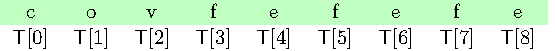
\includegraphics{kapitel/saca_algorithmen/bpr/algorithmus/phase1/t/image.pdf}\par\bigskip \\
			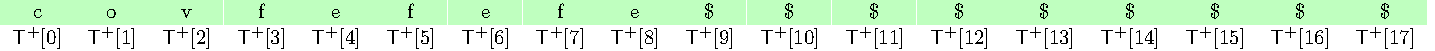
\includegraphics{kapitel/saca_algorithmen/bpr/algorithmus/phase1/tplus/image.pdf}
		\end{tabular}
	}
	\caption{Erweiterung von \inputtext zu \inputtextplus durch Anhängen von \(\$^n\)}
	\label{fig:tplus}
\end{figure}

\begin{definition}[\inputtextplus]
	\label{def:tplus}
    Sei \(\Sigma\) ein total geordnetes endliches Alphabet und \(\inputtext = \inputtext[0] \inputtext[1] \ldots \inputtext[n-1] \in \Sigma\) ein String über \(\Sigma\). Sei außerdem \(\$ \notin \Sigma\) ein nicht in \(\Sigma\) enthaltenes Symbol mit \(\forall c \in \Sigma : \$ < c\). Den um \(\$^n\) erweiterten String \(\inputtext\$^n\) nennen wir \inputtextplus.
\end{definition}

Ist das zugrunde liegende Alphabet außerdem total geordnet, so können auch die Suffixe eines Strings anhand dieser Ordnung sortiert werden.
Der Vergleich zweier Symbole des Alphabets bezüglich der Ordnung wird dadurch vereinfacht, dass jedem Symbol mit der Funktion \effective (Definition \ref{def:effective_alphabet}) eine natürliche Zahl als Rang zugewiesen wird.

Während für einzelne Symbole die Verwendung des effektiven Alphabets gegenüber dem direkten Vergleich keinen wesentlichen Vorteil erzielt, ergibt sich bei dem lexikographischen Vergleich zweier Strings bereits eine andere Situation: Auf Basis der Ränge der einzelnen Symbole kann auch ganzen Strings eine ganzzahlige Codierung zugewiesen werden, welche den Vergleich beschleunigt.

\begin{definition}[Stringkodierung]
	\label{def:coded}
	Sei \(\coded : (\Sigma \cup \{\$\})^d \rightarrow \{0, \ldots, (|\Sigma| + 1)^d - 1\}\) eine bijektive Funktion\footref{differs_from_paper}, sodass für zwei Strings \(u, v \in (\Sigma \cup \{\$\})^d\) gilt \(u < v \Leftrightarrow \coded(u) < \coded(v)\).
\end{definition}

Eine Stringkodierung wie in Definition \ref{def:coded} kann einfach unter Verwendung einer gegebenen \effective-Funktion (Definition \ref{def:effective_alphabet}) realisiert werden, indem die Symbole eines Strings abhängig von ihrem Index mit absteigender Wertigkeit für höhere Indizes summiert werden. Auf diese Weise ergibt sich für einen String \(\inputtext{[i,i+d)} = \inputtext[i] \ldots \inputtext[i + d - 1]\) die Kodierung \[\coded(\inputtext{[i,i+d)}) = \sum_{j=0}^{d - 1} (|\Sigma| + 1)^{d - 1 - j} \cdot \effective(\inputtext[i + j]).\]\par\smallskip
Auch Kodierungen für Strings größerer Länge als \(d\) können auf diese Weise berechnet werden, indem alle Symbole an Indizes größer oder gleich \(d\) ignoriert werden. Aufgrund der hier gewählten Berechnungsvorschrift für \coded lassen sich außerdem auf sehr einfache Weise Kodierungen für aufeinanderfolgende Suffixe berechnen.
\begin{equation}
	\label{eq:coded}
    \coded(\suffix{i+1}) = (|\Sigma| + 1) \cdot \left( \coded(\suffix{i}) \text{ mod } (|\Sigma| + 1)^{d-1}\right) + \effective(\inputtextplus[i+d])
\end{equation}
Man beachte hier, dass für zwei aufeinanderfolgende Suffixe \suffix{i} und \suffix{i+1} lediglich das erste Symbol aus \suffix{i} aus der Kodierung entfernt werden muss (mittels mod \((|\Sigma| + 1)^{d-1}\)), woraufhin die Wertigkeit aller verbleibenden Symbole jeweils um eine Stelle ansteigt. Zuletzt muss nur noch der Rang des letzten Symbols aus \suffix{i+1} hinzu addiert werden.\par\smallskip
Wie viele andere Algorithmen zur Konstruktion von Suffix-Arrays, arbeitet auch \bpr mit einer Unterteilung des Suffix-Arrays in sogenannte Buckets (Definition \ref{def:bucket} auf Seite \pageref{def:bucket}). Die Unterteilung des Arrays in Buckets ist erforderlich, um das Suffix-Array schrittweise sortieren zu können, indem bestehende Buckets durch Aufteilung weiter verfeinert werden.

\subsection{Algorithmus}
\label{bpr:algorithmus}

Nachdem in Kapitel \ref{bpr:vorueberlegungen} bereits die formalen Grundlagen für die Beschreibung des \bpr-Algorithmus geschaffen wurden, können wir nun präziser auf die Funktionsweise des Algorithmus eingehen. Die Basis für das Verfahren bildet die Nutzung von Abhängigkeiten zwischen mehreren Suffixen: Teilen sich zwei Suffixe \suffix{i} und \suffix{j} einen gemeinsamen Präfix der Länge \(\textit{offset}\), so ist zunächst festzustellen, dass \suffix{i+\textit{offset}} bzw. \suffix{j+\textit{offset}} nicht nur Suffixe von \inputtext, sondern auch Suffixe von \suffix{i} bzw. \suffix{j}  sind. Die Reihenfolge von \suffix{i} und \suffix{j} im Suffix-Array kann also einfach durch die Reihenfolge der eventuell bereits zuvor sortierten Suffixe \suffix{i+\textit{offset}} und \suffix{j+\textit{offset}} bestimmt werden. Um allerdings auf eine derartige Vorsortierung zurückgreifen zu können, muss zu Beginn zumindest eine grobe \glqq initiale Sortierung\grqq{} der Suffixe existieren.\par\smallskip
Um dies zu erreichen, verwendet der hier beschriebene Algorithmus zwei Phasen, von denen die erste dazu dient, die Suffixe initial nach gemeinsamen Präfixen der Länge \(d\) zu gruppieren. Auf Basis dieser Gruppierung werden die Suffixe Buckets zugewiesen, sodass sich zwei Suffixe genau dann im gleichen Bucket befinden, wenn sie einen gemeinsamen Präfix der Länge \(d\) besitzen.\par
In der zweiten Phase werden dann die Buckets anhand der oben genannten Vorschrift schrittweise rekursiv verfeinert. Auf diese Weise ergibt sich das fertig sortierte Suffix-Array, sobald jeder Bucket die minimale Länge von 1 erreicht hat.\par\smallskip
Im Folgenden werden beide Phasen im Detail erklärt. Wir verwenden dafür als Beispiel das Fantasiewort \covfefefe, dessen Suffixe wir mittels \bpr sortieren.

\input{kapitel/saca_algorithmen/bpr/algorithmus/phase1}
\input{kapitel/saca_algorithmen/bpr/algorithmus/phase2}
\input{kapitel/saca_algorithmen/bpr/algorithmus/beispiel}

\subsection{Effizienz}
\label{bpr:effizienz}

Im Bezug auf die Effizienz des hier beschriebenen Algorithmus muss zwischen der asymptotischen Worst-Case Analyse und der Effizienz in realen Anwendungsszenarien unterschieden werden. Es existieren bereits andere Verfahren mit sehr guten theoretischen Laufzeitschranken von \(\Theta(n)\) \cite{saca:9} (DC3, \cref{algorithm:dc3}) sowie praxisnähere Algorithmen mit einer Laufzeitkomplexität von \(\O(n \log n)\) \cite{saca:5} (DivSufSort, \cref{algorithm:divsufsort}), wobei \(n\) die Länge des Eingabestrings ist. Da es aber in der Praxis durchaus vorstellbar ist, dass Algorithmen mit schlechterer asymptotischer Laufzeit für reale Anwendungszwecke schneller sind, werden wir uns in \cref{ergebnisse} mit praktischen Laufzeitmessungen im Vergleich zu anderen Algorithmen auseinandersetzen.\par
Gerade in der Praxis ist allerdins nicht nur die Laufzeitkomplexität, sondern auch die Speicherkomplexität von hoher Bedeutung. Die nachfolgende Analyse beschäftigt sich daher insbesondere auch mit dem Speicherbedarf des \bpr-Algorithmus.

\input{kapitel/saca_algorithmen/bpr/effizienz/theorie}
%\input{kapitel/saca_algorithmen/bpr/effizienz/praxis}
\input{kapitel/saca_algorithmen/bpr/effizienz/modifikationen}

%\subsection{Fazit}
\label{bpr:fazit}

Wie wir gesehen haben, handelt es ich bei \bpr um einen Konstruktionsalgorithmus für Suffixarrays, der sich aufgrund seiner einfachen Struktur unkompliziert programmieren lässt. Darüber hinaus erzielt der Algorithmus besonders im Anwendungsgebiet der Bioinformatik gute Laufzeiten und eignet sich daher auch für den praktischen Einsatz.\par
Bei der Implementierung hat sich gezeigt, dass sich die Laufzeit des Algorithmus insbesondere durch die Verwendung von IPS\(^4\)o noch weiter beschleunigen lässt. Für die Umstrukturierung der Sortierphasen ist noch zu untersuchen, ob sich Fälle konstruieren lassen, in denen die geänderte Reihenfolge Nachteile gegenüber der originalen Version hat. Bisher konnten weder für kleine Eingaben, noch für große Dateien nennenswerte Unterschiede gemessen werden.\par\smallskip
Auf theoretischer Seite bleibt weiterhin von Interesse, ob die von Schürmann und Stoye beschriebene asymptotische Schranke von \(\O(n^2)\) \cite[Kapitel~5]{schuermann2005} auch für \(d < \log n\) eingehalten bzw. sogar noch verfeinert werden kann und welche Auswirkungen dies insbesondere auf den Speicherbedarf in Phase 1 des Algorithmus hat. Sollte die Schranke gültig sein, so ist zu analysieren, und ob für allgemeine Eingaben eventuell sogar eine kleinere obere Schranke existiert. Im Zuge dessen kann es hilfreich sein, komplexere Beispieleingaben zu konstruieren, die die Laufzeit des Verfahrens sowohl in der Rekursionstiefe als auch im Sortieraufwand maximieren.


\newpage
\section{mSufSort}

\subsection{Einleitung}

In \currentauthor{Rosa Pink} diesem Abschnitt wird ein Algorithmus, oder vielmehr eine Sammlung aus Algorithmen, vorgestellt, die in \glqq An Efficient, Versatile Approach to Suffix Sorting\grqq von Maniscalco et al. \cite{saca:8} beschrieben sind. Dabei liegt der Fokus nicht auf der exakten Wiedergabe des Papers, sondern auf weiterführenden Beispielen und Erläuterungen, sowie einer Erweiterung des dort bereits angegebenen Pseudocodes. Zudem wird auf die Implementierung im Rahmen der Projektgruppe eingegangen und ein Beispiel angehängt, das zum besseren Verständnis beitragen sollte. In einem weiteren Unterkapitel wird auf Möglichkeiten der naiven Parallelisierung eingegangen.\\

Bei der Entwicklung dieses Algorithmus wurden von Maniscalco et al. drei Ziele verfolgt:\\
1. \textbf{Kurze Laufzeit} - der Algorithmus soll mit anderen SACAs mithalten können. Er soll außerdem besonders schnell die Burrows-Wheeler Transformation~\cite{BWT} berechnen können, die zur verlustfreien Kompression von Texten verwendet werden kann.\\
2. \textbf{Wenig Platzverbrauch} im Arbeitsspeicher - Für Suffix Arrays existiert der Begriff \textit{lightweight} (leichtgewichtig), eingeführt von Manzini und Ferragina \cite{saca:4}. Er wird für SACAs verwendet, die nur einen Platzverbrauch von unter 6$n$ Bytes bei einer Länge des Eingabe-Strings von $n$ Zeichen haben. Dieser Platz wird für das Suffix Array (4$n$ Byte für $n < 2^{32}$) und zusätzlichen Arbeitsplatz verwendet.\\
3. \textbf{Sensitivität bezüglich dem Alphabet} - der Algorithmus sollte auch für große Alphabete $\Sigma$ funktionieren. Viele SACAs beschränken sich auf $|\Sigma| \leq 256$, damit auch $|\Sigma|^2$ noch eine händelbare Größe darstellt. In einigen Situationen ist das Alphabet jedoch größer, zB. für wortbasierte Burrows-Wheeler Transformation ist das Alphabet zwischen 20.000 bis 100.000 Zeichen groß, und asiatische Zeitungen oder Bücher enthalten üblicherweise über 10.000 verschiedene Zeichen \cite{asianAlphabets}. Im Rahmen der Projektgruppe werden jedoch nur Byte-Alphabete behandelt, dieser Aspekt wurde daher vernachlässigt.\\
Es werden (in Kapitel \ref{mainPart}) vier verschiedene Techniken eingeführt, deren Kombination schlussendlich den Kern des Algorithmus bildet:
\begin{enumerate}
\item $u$-Chain Bucket-Sort
\item Induziertes Sortieren
\item Erweitertes Induziertes Sortieren
\item Erkennen und Behandeln von Wiederholungen
\end{enumerate}
Da diese Techniken selbst alle noch kein Suffix Array konstruieren, muss anschließend noch eine der Varianten zur Umwandlung aus \ref{isa2sa} folgen. Ohne diesen Teil wäre der gesamte Algorithmus kein SACA im eigentlichen Sinne: Er konstruiert das Inverse Suffix Array \isa. Dieses enthält für jedes Suffix einen Rang, der die Position darstellt, an die es im Suffix Array sortiert werden soll. Während der Konstruktion des \isa werden in dem Speicherbereich des \isa zusätzlich weitere Komponenten des Algorithmus gespeichert, um Platz zu sparen.\\

\subsection{Bestandteile des Algorithmus und Pseudocode} \label{mainPart}
In diesem Kapitel wird der Algorithmus vorgestellt. Dazu wird er, wie von Maniscalco und Puglisi, in vier Abschnitte eingeteilt, die jeweils unterschiedliche Konzepte realisieren und alle dazu beitragen, dass der Algorithmus schneller wird. 
Obwohl die Abschnitte aufeinander aufbauen, kann schon ein Algorithmus der nur den ersten Abschnitt implementiert das \isa konstruieren. Im Originalpaper von Maniscalco und Puglisi wurden eine Version mit Abschnitt \ref{erwIndSort} und eine ohne diesen implementiert und im Anschluss experimentell mit anderen SACAs verglichen. Dabei stellte sich die Version mit erweitertem induzierten Sortieren als überlegen heraus.

\subsubsection{$u$-Chain Bucket-Sort}
\label{4.1}

Das erste Konzept, das in diesem Algorithmus Anwendung findet, ist eine Methode, bei der Suffixe sortiert werden. Dazu werden sogenannte $u$-Chains erstellt, verfeinert und abgearbeitet.
Eine $u$-Chain ist eine Kette aus Suffixen des Input-Strings \inputtext, die den selben Präfix $u$ haben. Die $u$-Chains sind daher eine Variante von Buckets, wie sie in \ref{def:bucket} definiert werden. Wenn $\mathsf{T}[i, i+|u|) = \mathsf{T}[j, j+|u|)$, so sind alle derartigen $i$ und $j$ in der selben $u$-Chain verlinkt. Ein Beispiel:
Der Input-String sei
\begin{center}
\begin{tabular}{c c c c c c c c c}
$i$ & 0 & 1 & 2 & 3 & 4 & 5 & 6 & 7 \\
$\mathsf{T}[i]$ & a & b & c & a & c & a & b & \$
\end{tabular}
\end{center}
Für $|u| = l = 1$ gibt es folgende $u$-Chains:
\begin{center}
\begin{tabular}{c c c c c}
$u$ & \$ & a & b & c \\
$u$-Chain & (7) & (5, 3, 0) & (6, 1) & (4, 2)
\end{tabular}
\end{center}
Falls eine $u$-Chain nur einen Eintrag hat, wie hier die \$-Chain, so spricht man von einem \textit{Singleton}.
$u$-Chains werden im \isa gespeichert:
\begin{center}
\begin{tabular}{c c c c c c c c c}
$i$ & 0 & 1 & 2 & 3 & 4 & 5 & 6 & 7 \\
$\mathsf{T}[i]$ & a & b & c & a & c & a & b & \$ \\
$\mathsf{ISA}[i]$ & $\perp$ & $\perp$ & $\perp$ & 0 & 2 & 3 & 1 & $\perp$
\end{tabular}
\end{center}
Sie sind nur von rechts nach links verlinkt und lassen sich auch nur in dieser Richtung durchlaufen.
Das Zeichen $\perp$ markiert jeweils das Ende einer $u$-Chain.
Um die Einträge, die $u$-Chains verlinken, im \isa von denjenigen Einträgen, die Ränge enthalten, zu unterscheiden, werden Ränge als negative Zahlen gespeichert. Wenn \isa[$i$] < 0 (bzw. das linkeste Bit ==1), dann gehört zu Suffix $i$ der Rang -\isa[$i$].

Die $u$-Chains, die bearbeitet werden sollen, werden als Tupel ($h$, $l$) aus dem Index des Kopfes (Head) der Chain $h$ und der Länge von $u$, $l$, auf einem Stack gespeichert.
Zu bearbeitende $u$-Chains liegen stets lexikographisch sortiert auf dem Stack, dh. diejenige $u$-Chain mit dem kleinsten $u$ liegt zuoberst.

\begin{listing}[htp]
\begin{minted}[numbers=left, escapeinside=@@]{python}
formInitialChains()
repeat:
  (h,l) @$\leftarrow$@ chainStack.pop()	
  if @\isa[h]@ = @$\perp$@:
    @\isa[h]@ @$\leftarrow$@ nextRank()		
  else:
    while h@$\neq \perp$@:
      sym @$\leftarrow$@ getSymbol(h+l)
      updateSubchain(sym, h)
      h @$\leftarrow$@ @\isa[h]@
    
    sortAndPushSubChains()	
until chainStack = @$\emptyset$@			
\end{minted}
\caption{$u$-Chain Bucket-Sort.}
\label{uChain}
\end{listing}

In Algorithmus \ref{uChain} (aus \cite{saca:8}) wird der Pseudocode des $u$-Chain Bucket-Sort mSufSort dargestellt.
Zu Beginn werden die initialen $u$-Chains der Länge 1 gebildet und sortiert auf den Stack gelegt. Danach werden solange $u$-Chains auf dem Stack abgearbeitet, bis dieser leer ist, und damit alle Suffixe im \isa einen Rang zugewiesen bekommen haben.
Es wird in jedem Schleifendurchlauf ein $u$-Chain-Tupel vom Stack genommen. Handelt es sich dabei um ein Singleton, so wird direkt ein Rang zugewiesen. Wenn die $u$-Chain mehrere Einträge hat, so wird die $u$-Chain \textit{verfeinert}. Das bedeutet, es werden Sub-Chains erstellt die jeweils ein Zeichen mehr berücksichtigen. Die Länge von $u$ erhöht sich also um 1. Diese Sub-Chains werden dann, sobald die $u$-Chain durchlaufen wurde, sortiert und auf den Stack gelegt. Daher werden sie im nächsten Durchlauf als erstes abgearbeitet, und sollten durch die Verfeinerung Singletons entstanden sein, werden diese nun entsprechend Ränge zugewiesen bekommen.\\

Ein auf direkten Vergleichen basierendes Bucket-Sorting reicht allein für einen konkurrenzfähigen SACA noch nicht aus (vgl. \cite{seward2000}).

\subsubsection{Induziertes Sortieren}

In diesem Abschnitt wird die Grundidee des Induzierten Sortieren erläutert, wie sie hier verwendet wird. In \cref{section:induzierer} wird dieses Konzept noch allgemeiner erklärt. 
Grob gesagt gibt es viele Suffixe, deren Ränge abhängig von den Rängen anderer Suffixe sind, und diese Abhängigkeit kann zum schnelleren Sortieren genutzt werden.
Man sagt, Suffix $i$ aus einer $u$-Chain der Länge \ell lässt sich \textit{induziert} sortieren, wenn der Rang für Suffix $i+l$ bereits bekannt ist.
Es kann beobachtet werden, dass solche induziert sortierbaren Suffixe lexikographisch vor den anderen Suffixen kommen: sie haben offensichtlich selbst lexikographisch kleinere Sub-Suffixe, als andere Suffixe mit dem selben Präfix $u$.
Bei der Verfeinerung der $u$-Chains werden nun nur noch nicht-induziert sortierbare Suffixe in Sub-Chains platziert, während die induziert sortierbaren Suffixe anders sortiert werden. Die Reihenfolge dieser induziert sortierbaren Suffixe lässt sich mittels vergleichsbasiertem Sortieren bestimmen, indem der Rang von Suffix $i+l$ als Sortierschlüssel genutzt wird. Sobald die Menge $M$ ($|M| = m$) der induziert sortierbaren Suffixe nach den Sortierschlüsseln sortiert wurde, werden diesen Suffixen die nächsten $m$ Ränge zugewiesen. Diese Art des Sortierens für Suffixe nennen wir (hier) \textit{Induziertes Sortieren}.\\

Im Pseudocode (Algorithmus \ref{indSort}, aus \cite{saca:8}) wird jetzt der Ansatz des Bucket-Sort um Induziertes Sortieren erweitert. Es wird nun direkt nach dem Check auf ein $u$-Chain-Singleton geprüft, ob sich der Eintrag der $u$-Chain per Induktion sortieren lässt (Zeile 8). Falls dies der Fall ist, wird das Suffix mit dem Sortierschlüssel annotiert. Am Ende einer $u$-Chain wird dann nach der Verfeinerung der Chains die Menge der annotierten Suffixe sortiert und gerankt.

\begin{listing}[htp]
\begin{minted}[numbers=left, escapeinside=@@]{python}
formInitialChains()
repeat:
  @$(h,l) \leftarrow$@ chainStack.pop()	
  if @\isa[h]@ = @$\perp$@:
    @\isa[h]@ @$\leftarrow$@ nextRank()		
  else:
    while @$h\neq \perp$@:
      if isRanked(@$h+l$@)
        noteSuffix(h, @\isa[h+l]@)
      else:
      sym @$\leftarrow$@ getSymbol(@$h+l$@)
      updateSubchain(sym, @$h$@)
      
      @$h \leftarrow$@ @\isa[h]@
   
    pushSubChains()	
    rankNotedSuffixes()
  				
 until chainStack = @$\emptyset$@
\end{minted}
\caption{Induziertes Sortieren.}
\label{indSort}
\end{listing}

\subsubsection{Erweitertes Induziertes Sortieren} 
\label{erwIndSort}

In diesem Abschnitt wird die Idee des Induzierten Sortierens weitergeführt, um die Laufzeit des mSufSort weiter zu verbessern.
Dazu wurde überlegt, dass sich alle Suffixe direkt zu Beginn in zwei Gruppen unterteilen lassen: Typ S (smaller) und Typ L (larger).\\
Suffix $i$ ist von Typ L, wenn es größer als das nächste Suffix $i+1$ ist: T$[i] >$ T$[i+1]$, oder im Falle von Gleichheit wird das nächste Zeichen inspiziert und mit $T[i]$ verglichen, bis schließlich T$[i] >$ T$[i+j]$. Andernfalls (falls entweder T$[i] <$ T$[i+1]$ oder bei Gleichheit dann T$[i] <$ T$[i+j]$) ist es von Typ S. Alle Suffixe $i$ von Typ L kommen vor Suffixen $j$ mit Typ S, die den gleichen Anfangsbuchstaben T$[i] =$ T$[j]$ haben: T$[i,n] <$ T$[j,n]$.
\\
Das bedeutet für Suffix $i$, dass sich sein Rang später von dem Rang des Suffix $j$ ableiten lassen wird. Daher wird die gesamte Prozedur des Bucket-Sort und Induzierten Sortierens jetzt nur noch auf Typ S Suffixe angewandt, während Typ L Suffixe mit einer neuen Methode sortiert werden.
Und zwar fügen wir immer, wenn Suffix $i$ ein Rang zugewiesen wird, und Suffix $i-1$ von Typ L ist, Suffix $i-l$ am Ende einer Liste $M_{\alpha\beta}$ ein, ganz konkret der  Liste $M_{T[i-1]T[i]}$ (aufgrund von Typ L-Eigenschaft gilt für alle $M_{\alpha\beta}$: $\alpha \leq \beta$). 
Alle Listen $M_{\alpha\beta}$ zu einem gegebenen $\alpha$ und beliebigen $\beta$ werden genau dann gerankt, wenn auf dem Stack die $u$-Chain mit Tupel $(h, l)$ erreicht wird, deren $T[h] = \alpha$.


\begin{listing}[htp]
\begin{minted}[numbers=left, escapeinside=@@]{python}
classifyTypeUV()
formInitialChains(Type U suffixes)
initializeVLists()
repeat:
  @$(h,l)$@ @$\leftarrow$@ chainStack.pop()	
  for all @$M_{T[h]\beta} \ \in$@ VLists[@\inputtext[h]@] @$\neq \perp$@} in lexicographical order :
    rankAll(@$M_{T[h]\beta}$@)
  
  if @\isa[h]@ = @$\perp$@ :
    @\isa[h]@ @$\leftarrow$@ nextRank()		
  else:
    while @$h\neq \perp$@ :
      if isRanked@$(h+l)$@ :
        noteSuffix(@$h$@, @\isa[h+l]@)
      else:
      sym @$\leftarrow$@ getSymbol@$(h+l)$@
      updateSubchain(sym, @$h$@)
      
      @$h \leftarrow$@ @\isa[h]@
	
    pushSubChains()	
    rankNotedSuffixes()
  
  if chainStack = @$\emptyset$@ :
    activeVLists @$\leftarrow$@ VLists @$\neq \perp$@
    rankAll(activeVLists)
    if activeVLists = @$\emptyset$@ :
      return
  		
\end{minted}
\caption{Erweitertes Induziertes Sortieren.}
\label{erwIndSort}
\end{listing}

Im Pseudocode (Algorithmus \ref{erwIndSort}) wird nicht näher auf dieses Einfügen in die Listen $M_{\alpha\beta}$, das beim Ranken passiert, eingegangen, um die Übersichtlichkeit zu bewahren. Ganz zu Anfang werden die Suffixe jetzt allerdings in Typ S und Typ L unterschieden, wobei von Maniscalco und Puglisi vorgeschlagen wird, Typ L-Suffixe durch das Zeichen $\perp$ im \isa zu kennzeichnen. Beim Bilden der $u$-Chains werden dann nur die Typ S-Suffixe verwendet. Es muss eine Datenstruktur, die die Heads und Tails der Listen $M_{\alpha\beta}$ verwaltet, wir nennen sie hier VLists, initialisiert werden. Es wäre praktisch, wenn diese Datenstruktur die Listen bereits in lexikographischer Sortierung speichert. Auch wäre praktisch, wenn zudem Buch darüber geführt wird, ob Elemente in einer Liste enthalten sind, oder ob diese leer ist. Der Zugriff auf alle Listen $M_{\alpha\beta}$ zu einem gegebenen $\alpha$ und beliebigen $\beta$ wird hier einfach VLists[$\alpha$] genannt.
Maniscalco und Puglisi schreiben, der Inhalt der Listen $M_{\alpha\beta}$ lässt sich wieder im \isa speichern. Die Datenstruktur VLists hat daher eine Größe die in O($|\Sigma|^2$) liegt, bzw. genauer bei maximal $\frac{|\Sigma|*(|\Sigma|-1)}{2}$.
Für große Alphabete, so argumentieren die Autoren, sei die Idee erweiterbar, indem für jedes Symbol nur noch zwei Listen verwaltet werden; $M_\alpha$ für Suffixe mit Präfix $\alpha\beta$ wobei $\alpha \neq \beta$, und eine Liste mit $M_{\alpha\alpha}$.\\
Für Datensätze, bei denen Typ S Suffixe häufiger sind, kann man den Ansatz optimieren, indem man dann die Rollen der Typen umkehrt. Dafür muss man vor allem beachten, dass die Ränge dann auch anders herum verteilt werden müssen (absteigend statt aufsteigend).

\subsubsection{Erkennen und Behandeln von Wiederholungen}

In diesem Abschnitt wird die letzte und wohl komplizierteste Erweiterung des mSufSort erklärt: Der Umgang mit Wiederholungen im Input-Array. Dazu muss man zunächst wissen, dass es für vergleichsbasiertes Sortieren, wie es beim Bucket-Sort verwendet wird, sehr ungünstig ist, wenn sich Sequenzen wiederholen, wie zB.: \glqq abcabcabc\grqq{}. Für eine $abc$-Chain hätte man hier drei aufeinanderfolgende Einträge, jedoch beim Verfeinern immer noch zwei mal die Sequenz $abca$. Je länger diese Wiederholungssequenz, desto ungünstiger (da immer öfter weitere Verfeinerung zu Sub-Chains nötig wird).
Auf der anderen Seite hat man mit den $u$-Chains schon ein mächtiges Tool, mit dem sich eben solche Sequenzen erkennen lassen, und kann dann die Wiederholungen aus den Verfeinerungen ausschließen und anders sortieren.\\
Wir definieren eine Wiederholungssequenz $S_{i,u}$ als Sequenz, die bei Index $i$ (von rechts) beginnt, und jeweils den String $u$ der Länge $l$ direkt hintereinander enthält:
T$[i, i+l]=$T$[i+l+1, i+2l]=...$
Am letzten Beispiel: der String 
\begin{center}
\begin{tabular}{c c c c c c c c c c c}
$i$ & 0 & 1 & 2 & 3 & 4 & 5 & 6 & 7 & 8 & 9\\
T$[i]$ & a & b & c & a & b & c & a & b & c & \$\\
\end{tabular}
\end{center}
entspricht einer Wiederholungssequenz $S_{7,abc} = abc^3$.
Folgendes ist dagegen keine Wiederholungssequenz:
\begin{center}
\begin{tabular}{c c c c c c c c c c c}
$i$ & 0 & 1 & 2 & 3 & 4 & 5 & 6 & 7 & 8 & 9\\
T$[i]$ & a & b & d & a & b & c & a & b & a & \$\\
\end{tabular}
\end{center}
Hier kommen zwar die Buchstabenkombinationen \glqq ab\grqq{} oft vor, aber es sind Lücken zwischen den $u$-Strings, mit unterschiedlichen Zeichen.
Man unterscheidet bei einer Wiederholungssequenz zwischen der sogenannten \textit{terminierenden} Position und den {nicht-terminierenden} Positionen. Die terminierende Position entspricht genau dem $i$ zu $S_{i,u}$, also dem rechtesten Beginn des wiederholt auftretenden Substrings $u$. Alle weiteren Positionen $j$, wobei $j = i-r\cdot |u|$, die den Beginn weiterer Substrings $u$, die weiter links liegen, anzeigen, sind nicht-terminierend.\\
Diese Unterscheidung wird getroffen, weil sich alle nicht-terminierenden Positionen direkt anhand der Ränge der terminierenden Positionen bestimmen lassen. Es gilt für Wiederholungssequenzen $S_{i, u}$ (mit $|u|=l$), deren terminierende Position, Suffix $i$, sich induktiv sortieren lässt, dass \inputtext[i, n] $<$ \inputtext[i-l, n] $< ... <$ \inputtext[i-l(|S|-1), n].
Die Ränge der nicht-terminierenden Positionen werden also aufsteigend, beginnend bei der terminierenden Position, von rechts nach links vergeben.
Im umgekehrten Fall, wenn Suffix $i$ nicht induziert sortierbar ist, werden die Ränge genau anders herum vergeben: \inputtext[i, n] > \inputtext[i-l, n] $> ... >$ \inputtext[i-l(|S|-1)].
Wenn sich ein Suffix $i$ induziert sortieren lässt, so bedeutet das, dass der Buchstabe hinter dem Präfix $u$ kleiner ist, als Zeichen \inputtext[i], oder zumindest höchstens gleich groß, und das Suffix $i+l$ kleiner ist. Ansonsten wäre dieses Suffix nicht vorher gerankt worden. Daher kommt im Induktionsfall das Suffix an terminierender Position zuerst. Lässt sich das Suffix $i$ dagegen nicht induziert sortieren, dann muss das Zeichen (bzw. mindestens aber das Suffix) $i+l$ größer sein, da es nicht vorher abgearbeitet wurde. In diesem Fall ist das Suffix an terminierender Position also das mit dem höchsten Rang. 
Zwei Beispiele, um die Regeln zu verdeutlichen:
Sei $y$ der zuletzt vergebene Rang zum Zeitpunkt der Rangzuweisung an die Suffixe der Wiederholungssequenz. Zunächst der Fall, in dem sich per Induktion der Rang von Suffix $i$ bestimmen lässt, wobei \inputtext[i] = \inputtext[i+l] und erst \inputtext[i+1] > \inputtext[i+l+1].
\begin{center}
\begin{tabular}{c c c c c c c c c c c c c}
Rang & Suffix\\
$y$ + 1 & \inputtext[i, n] & a & b & c & \cellcolor{black!20!white}a & \cellcolor{black!20!white}\$\\
$y$ + 2 & \inputtext[i-l, n] & a & b & c & \cellcolor{black!20!white}a & \cellcolor{black!20!white}b & c & \cellcolor{black!20!white}a & \cellcolor{black!20!white}\$\\
$y$ + 3 & \inputtext[i-2l, n] & a & b & c & a & b & c & \cellcolor{black!20!white}a & \cellcolor{black!20!white}b & c & a & \$
\end{tabular}
\end{center}
Nun der andere Fall.
\begin{center}
\begin{tabular}{c c c c c c c c c c c c c}
Rang & Suffix\\
$y$ + 3 & \inputtext[i, n] & a & b & c & \cellcolor{black!20!white}d & \$\\
$y$ + 2 & \inputtext[i-l, n] & a & b & c & \cellcolor{black!20!white}a & b & c & \cellcolor{black!20!white}d & \$\\
$y$ + 1 & \inputtext[i-2l, n] & a & b & c & a & b & c & \cellcolor{black!20!white}a & b & c & d & \$
\end{tabular}
\end{center}
In einer $u$-Chain können leider mehr als eine Wiederholungssequenz vorkommen, so sind zum Beispiel die Sequenzen $S_{6, ab}$ und $S_{0, ab}$ in dieser $ab$-Chain enthalten:
\begin{center}
\begin{tabular}{c c c c c c c c c c c}
$i$ & 0 & 1 & 2 & 3 & 4 & 5 & 6 & 7 & 8 & 9\\
\inputtext[i] & a & b & a & b & \cellcolor{black!20!white}c & a & b & a & b & \cellcolor{black!20!white}\$\\
\end{tabular}
\end{center}

Schon dieser Fall ist komplexer. Die Ränge für $S_{6,ab}$ können direkt zugewiesen werden, da \$ vorher gerankt wurde. Dadurch, dass dann nur noch eine terminierende Position, Suffix $2$, in der Sub-Chain enthalten ist, wird schließlich diese Wiederholungssequenz gerankt, beginnend bei Suffix $0$.
Offen ist noch was geschieht in dem Fall, dass zwei Wiederholungssequenzen sich induziert sortieren lassen: Dann werden die Ränge der nicht-terminierenden Positionen \textit{interleaved} (englisch für \glqq in einander verzahnt\grqq{}). Das bedeutet, dass die Ränge der nicht-terminierten Positionen abwechselnd für alle induziert sortierbaren Wiederholungssequenzen vergeben werden, und zwar entsprechend der Reihenfolge der Ränge der terminierten Positionen. Am Beispiel zweier Wiederholungssequenzen $S_{i,u}$ und $S_{j,u}$: Sei Suffix $i$ < Suffix $j$. Dann folgt: $rank(i-l) < rank(j-l) < rank(i-2l) < rank(j-2l) < ...$ und so weiter, bis zur letzten nicht-terminierten Position aus Suffix $j$.\\
Es bleibt der Fall, wenn mehrere Wiederholungssequenzen der selben $u$-Chain sich nicht per Induktion sortieren lassen. Dies ist der komplizierteste Fall. Hier wird nämlich zunächst eine Liste aus allen nicht-terminierenden Positionen der Wiederholungssequenzen, $C$, auf den Chainstack gelegt. Die terminierenden Positionen werden in Sub-Chains eingeordnet. Solange sich allerdings eine Liste $C$ auf dem Stack befindet, werden keine Ränge zugewiesen, sondern es wird eine Liste $Q$ gefüllt, indem jedes Suffix, das sonst gerankt werden würde, ans Ende der Liste gehängt wird. Sobald $C$ dann oben auf dem Stack liegt, wird die Reihenfolge der terminierenden Positionen aus $Q$ genutzt, um die Suffixe aus $C$ zu sortieren. Dabei wird ebenfalls interleaved, wie bei den induziert sortierbaren Wiederholungssequenzen - entsprechend anders herum. Maniscalco und Puglisi schreiben, um $C$ und $Q$ zu implementieren, werde nur konstanter zusätzlicher Speicherplatz benötigt, um Beginn und Ende der Listen zu speichern, während die eigentlichen Verlinkungen wieder im \isa gespeichert sind. Der Pseudocode (Algorithmus \ref{wiedSeq}) dient nur der besseren Einordnung in den gesamten Algorithmus, da die Wiederholungserkennung (und -behandlung) an verschiedene Stellen verteilt wird.

\begin{listing}[htp]
\begin{minted}[numbers=left, escapeinside=@@]{python}
classifyTypeUV()
formInitialChains(Type U-suffixes)
initializeVLists()
initializeQ()
repeat:
  if typeOf(chainStack.peak()) @$\neq$@ @$u$@-Chain :
    C @$\leftarrow$@ chainStack.pop()
    cOnStack @$\leftarrow$@ FALSE
    rankBy(C, Q)
    rank(Q) 
  @$(h,l)$@ @$\leftarrow$@ chainStack.pop()	
  for all @$M_{\alpha\beta} \ \in$@ VLists[@\inputtext[h]@] @$\neq \perp$@} :
    rankAll(@$M_{\alpha\beta}$@)  
  if @\isa[h]@ = @$\perp$@ & not cOnStack :
    @\isa[h]@ @$\leftarrow$@ nextRank()	
  else if @\isa[h]@ = @$\perp$@ :
    Q @$\leftarrow h$@	
  else :
    while @$h\neq \perp$@ :   
      if isInRepSeq(@$h$@):
        if toBeInterleaved:
          noteNTSuffix(@$h$@)
        else:
          updateC(@$h$@)          
        if isEndOfRepSeq(@$h$@):
          toBeInterleaved @$\leftarrow$@ FALSE      
      else :
        if isRanked(@$h+l$@) :
          noteSuffix(@$h$@, @\isa[h+l]@)
          if isHeadOfRepSeq(@$h$@):
            toBeInterleaved @$\leftarrow$@ TRUE       
        else :
          sym @$\leftarrow$@ getSymbol(@$h+l$@)
          updateSubchain(sym, @$h$@)
          if isHeadOfRepSeq(@$h$@):
            C @$\leftarrow$@ createC(@$h, l$@)
      @$h \leftarrow$@ @\isa[h]@	
	  if(C@$\neq \emptyset$@) :
	    pushC()
	    cOnStack @$\leftarrow$@ TRUE	    
      pushSubChains()	
      rankNotedSuffixes()
      rankNotedNTSuffixes()   	
    if chainStack = @$\emptyset$@ :
      activeVLists @$\leftarrow$@ VLists @$\neq \perp$@
      rankAll(activeVLists)
        if activeVLists = @$\emptyset$@:
          return
\end{minted}
\caption{Wiederholungserkennung und -behandlung.}
\label{wiedSeq}
\end{listing}


\subsection{Weitere Details} \label{Details}

In diesem Kapitel finden sich alle wichtigen Details, die sich keinem speziellen Konzept zuordnen ließen, wie zum Beispiel dem grundlegenden Sortierverfahren, das an einigen Stellen (insbesondere Bucket-Sort) seine Anwendung findet. Aber auch ein paar erweiternde Ideen, zB. zur Steigerung der Effizienz des Bucket-Sort, werden hier vorgestellt.
Es ist jedoch keine vollständige Wiedergabe des Kapitels 5 über \glqq Entwicklungs- und Implementierungsdetails\grqq{} aus \cite{Maniscalco}.

\subsubsection{Sortierverfahren}

Für vergleichsbasiertes Sortieren wird Introsort (siehe \ref{section:introsort}) verwendet. Zudem wird zur Optimierung Insertion-Sort für besonders kleine Partitionen genutzt, wo es schneller als Quicksort ist.\\

\subsubsection{Eingabe-Transformation}

Es macht Sinn, das Alphabet wenn möglich kompakter darzustellen, wie auch in \ref{section:effalphabet} erläutert. Dazu wird es umcodiert auf fortlaufende Zahlenwerte 0..$|\Sigma|-1$. Das \$-Zeichen wird nicht explizit ins Alphabet aufgenommen, da dem $n$-ten Suffix sein Rang direkt zu Beginn zugewiesen werden kann. Es wird nie zum Vergleich benötigt, da alle Suffixe, die es im Zuge von Bucket-Sort betrachten wollten bereits per Induktion sortiert werden können mit dem Rang als Sortierschlüssel.

\subsubsection{Erweiterung für Bucket-Sort}

Das Bucket-Sort lässt sich verbessern, indem statt nur einem Symbol jeweils zwei Symbole (sogenannte \textit{Bigramme}) auf einmal betrachtet werden (siehe auch Abschnitt \ref{section:effalphabet}). Für kleine Alphabete mit $|\Sigma| \leq 256$ ist $|\Sigma|$ noch klein genug. Nicht nur werde durch das Kombinieren zweier Zeichen String-Sortieren beschleunigt, sondern es sei so auch möglich mehr Suffixe per Induktion zu sortieren (siehe nächsten Abschnitt).

\subsection{Erweiterung für (einfaches) Induziertes Sortieren}

Während dem Induzierten Sortieren werden Index des per Induktion zu sortierenden Suffix und der zugehörige Sortierschlüssel laut Pseudocode annotiert. Dazu werden Index und Schlüssel direkt nebeneinander in einem eigenen, dynamischen Array gespeichert, so Maniscalco und Puglisi. Dadurch werden unnötige Cache-Misses vermieden, was den Algorithmus beschleunigt. Allerdings wird dafür Speicherplatz benötigt, und zwar 8$m$ Byte für $m$ Suffixe die gerade per Induktion sortiert werden sollen. In der Praxis sollte $m$ deutlich kleiner als $n$ sein, insbesondere nachdem das Alphabet kompakter gemacht wurde.
Für den Fall, dass diese 8$m$ Byte problematisch werden könnten, schlagen Maniscalco und Puglisi zwei Alternativen vor; im einen Fall wird nur der Index des per Induktion zu sortierenden Suffixes gespeichert (mit 4$m$ Byte Speicherplatz). Der andere Fall ist etwas komplexer, benötigt aber nur 2$n$+o($n$) Bits Speicher. Diese Methode wurde nicht tatsächlich in die Implementierung aufgenommen.\\
Durch das Betrachten von zwei Zeichen auf einmal kann nun während eine Chain mit Länge des gemeinsamen Präfix \ell bearbeitet wird in drei Typen von Suffixen unterschieden werden: Suffix $i$ ist von Typ A, wenn der Rang von Suffix $i+l-1$ bekannt ist. Es ist von Typ B, wenn der Rang von Suffix $i+l$ bekannt ist -- und von Typ C ansonsten. Lexikographisch sind nun Typ A Suffixe kleiner als Typ B Suffixe, und diese wiederum kleiner als Typ C Suffixe. Es kann nun zuerst die Reihenfolge der Typ A Suffixe mittels Induziertem Sortieren bestimmt werden. Danach bestimmt man auf die selbe Art die Reihenfolge der Typ B Suffixe. Tatsächlich lässt sich dies in einem einzigen Aufruf kombinieren, indem als Sortierschlüssel für Typ B Suffixe nicht $i+l$ sondern $-(i+l)$ verwendet wird.

\subsection{Eigene Implementierung und Ausblick}
In unserer Implementierung des mSufSort haben wir $u$-Chain Bucket-Sort, Induziertes Sortieren und Erweitertes Induziertes Sortieren umgesetzt. Viele kleinere Ungenauigkeiten in der Beschreibung mussten dafür zunächst geklärt werden, zum Beispiel die verwendeten Datenstrukturen betreffend.
Die Erkennung und Behandlung von Wiederholungen ist teilweise implementiert worden, für den einfacheren Fall in dem sich Wiederholungssequenzen induziert sortieren lassen.
Die größte Herausforderung bei der Implementierung ist wohl der Umgang mit den einfach verlinkten Listen, die unter Anderem (aber nicht nur) für $u$-Chains verwendet werden. Diese selbstgebaute Datenstruktur ist sehr fehleranfällig, da komplexe Operationen benötigt werden, zB. Einfügen noch während über die Liste iteriert wird.\\

Sämtliche hier beschriebene Optimierungen, bis auf die Verwendung eines effektiven Alphabets, wurden noch nicht implementiert, dafür wurde allerdings bei der initialen Befüllung des Chainstacks ein Trick angewandt. 
Statt diese nämlich über eine $u$-Chain Verfeinerung mittels Introsort (auf einer Eingabelänge von O($n$)) zu lösen, wurde ein Array der Größe O($|\Sigma|$) eingeführt. Dieses enthält immer das rechteste Element einer $u$-Chain zum Zeitpunkt der Bearbeitung, dh. nach einem kompletten Scan von links nach rechts enthält es in sortierter Reihenfolge alle Elemente, die so direkt auf den Chainstack geschrieben werden können.
Dadurch konnte der Speicherverbrauch im Vergleich zur Referenzimplementierung noch deutlich gesenkt werden. Erst für Alphabete, deren Größe die Anzahl der Typ S-Suffixe übersteigt, lohnt diese Optimierung nicht.\\

Eine weitere Optimierung könnte, solange keine Wiederholungserkennung benötigt wird, noch darin bestehen, die Sortieroperation für $u$-Chains zu vereinfachen, indem diese nicht mehr konsequent geordnet verlinkt werden, sondern auch chaotisch gelinkt werden darf. Dies würde eine Wiederholungserkennung, wie im Originalpaper beschrieben, unmöglich machen, aber sicher einige Laufzeit einsparen.\\

Auch wäre noch denkbar, ein Sortierverfahren zu verwenden, das direkt auf den einfach verlinkten Listen funktioniert, statt jeweils die Liste zu durchlaufen und damit einen Vektor zu befüllen, bevor darauf Introsort angewandt werden kann.\\

Zur Zeit verwenden wir den naiven Inplace Ansatz zur Umwandlung des \isa zu \sa - es ist daher noch mit weiterer Verbesserung der Laufzeit zu rechnen, wenn andere Varianten eingebaut werden, auch wenn diese auf Kosten des Speicherverbrauchs gehen wird.


\subsection{Fazit}

Dieser Ansatz zur Sortierung von Suffixen legt den Fokus nicht auf die Erzeugung des Suffix Arrays, sondern es wird statt dessen das Inverse Suffix Array gebildet, aus dem sich direkt effizient die Burrows-Wheeler-Transformation (eine Anwendung für SACAs) ableiten lässt.
Dadurch unterscheidet sich dieser SACA ganz grundlegend von den meisten anderen Algorithmen, die direkt Suffix-Indizes verschieben, statt Ränge zu berechnen.\\
Insgesamt kann man dabei eigentlich dennoch nicht von einem Ansatz sprechen, dieser Algorithmus vereint vier verschiedene Konzepte in einem, man könnte sogar sagen fünf (mit dem Zusammenfassen zu Zeichenpaaren, Kapitel \ref{Details}). Dadurch wird er leider etwas unübersichtlich. Auch die Mehrfachnutzung des \isa als Platz für diverse andere Datenstrukturen (verlinkte Listen) ist für eine bessere Verständlichkeit -- sowie einfache Implementierung -- nicht hilfreich. Aufgrund zahlreicher solcher Tricks wird, falls 32bit Typen verwendet werden, die Eingabegröße beschränkt auf $n < 2^{31}$ (durch negative Ränge). Bei Anwendung des empfohlenen, da schnellsten, Verfahrens zur Erzeugung des Suffix Arrays, wird die Eingabegröße sogar auf $n < 2^{30}$, unter Umständen sogar auf $n < 2^{29}$ beschränkt. Das sind nur noch $\frac{1}{8}$ der ursprünglichen (und üblichen) $2^{32}$ Zeichen.\\
Auf der anderen Seite kann mSufSort mit anderen SACAs, wie zB. Deep-Shallow~\cite{saca:4}, was Laufzeit und Speicherverbrauch angeht, mithalten, wie Experimente von Maniscalco und Puglisi zeigen konnten. Eine formale Laufzeitanalyse liegt zwar nicht vor, aber die Autoren schreiben, sie vermuten eine Schranke von $\Theta(n^2 log(n))$. Sie geben einen Speicherverbrauch von \glqq etwas mehr als\grqq{} 4$n$ + $zn$ Byte an. Der tatsächliche Speicherverbrauch in den Experimenten liegt bei etwa 5-6$n$ Byte, wobei beachtet werden muss, dass dies nur der Fall ist, wenn bei der Konstruktion des Suffix-Array der Eingabe-String überschrieben werden darf. Andernfalls muss mit Abstrichen in der tatsächlichen Laufzeit oder einem deutlichen Wachstum des benötigten Speicherplatzes gerechnet werden. Allgemein liegt bei dem Algorithmus eine Trade-Off Situation zwischen Speicherplatz und Laufzeit vor. Mit mehr Speicherplatz ließen sich unter anderem einige Konzepte deutlich Cache-freundlicher umsetzen.
Der Algorithmus mSufSort scheint außerdem recht robust gegenüber dem Auftreten von Wiederholungen in der Eingabe zu sein. Ein weiterer Vorteil kann darin gesehen werden, dass es möglich ist, den Algorithmus (mit einigen Anpassungen) auch für große Alphabete mit $|\Sigma| > 256$ zu nutzen.\\
Der ursprüngliche Algorithmus, wie er hier beschrieben wurde, wurde inzwischen erweitert, es existiert nun auch eine parallelisierte Version von Maniscalco (unter \url{https://github.com/michaelmaniscalco/msufsort}).

\subsection{Beispiel}
Hier ein Beispiel, das zum Verständnis des Ablaufs im Algorithmus beitragen sollte.

\subsubsection{Initialisierung}
\textbf{Typen L und S} (bzw. V und U entsprechend) bestimmen,
und $u$-Chains mit $|u| = 1$ aus Typ U (S) bilden:
\begin{center}
\begin{tabular}{c c c c c c c c c c c c c c c c}
$i$ & 0 & 1 & 2 & 3 & 4 & 5 & 6 & 7 & 8 & 9 & 10 & 11 & 12 & 13 & 14\\
\inputtext[i] & c & a & a & b & a & c & c & a & a & b & a & c & a & a & \$\\
\isa[$i$] & V & $\perp$ & 1 & V & 2 & V & V & 4 & 7 & V & 8 & V & V & V & $\perp$
\end{tabular}
\end{center}

Heads der $u$-Chains als Tupel ($h$,$l$) (mit $h$ Index des rechtesten Elements der Chain, $l = |u|$) sortiert auf den Chain-Stack legen (Sortieren immer mit \textbf{Introsort}, für kleine Partitionen Insertionsort):\\
\textbf{chainStack:} \begin{itemize} \item (14, 1) - \$ \item (10, 1) - a \end{itemize}

\subsubsection{Hauptschleife}

Nehme Tupel vom Stack: (14, 1).\\
Eintrag bei Index 14 im \isa ist $\perp$, also weise ersten Rang zu:\\
\begin{center}
\begin{tabular}{c c c c c c c c c c c c c c c c}
$i$ & 0 & 1 & 2 & 3 & 4 & 5 & 6 & 7 & 8 & 9 & 10 & 11 & 12 & 13 & 14\\
\inputtext[i] & c & a & a & b & a & c & c & a & a & b & a & c & a & a & \$\\
\isa[$i$] & V & $\perp$ & 1 & V & 2 & V & V & 4 & 7 & V & 8 & V & V & V & -0
\end{tabular}
\end{center}

Prüfe, ob Eintrag ISA[$h-1$] V ist: Ja.\\
Speichere Index 13 in $M_{a\$}$ (im ISA - nur Head/Tail der Liste extra)\\
Bearbeite alle (nicht-leeren) Listen $M_{a*}$: Weise Suffix 13 den nächsten Rang zu.
\begin{center}
\begin{tabular}{c c c c c c c c c c c c c c c c}
$i$ & 0 & 1 & 2 & 3 & 4 & 5 & 6 & 7 & 8 & 9 & 10 & 11 & 12 & 13 & 14\\
\inputtext[i] & c & a & a & b & a & c & c & a & a & b & a & c & a & a & \$\\
\isa[$i$] & V & $\perp$ & 1 & V & 2 & V & V & 4 & 7 & V & 8 & V & V & -1 & -0
\end{tabular}
\end{center}

Prüfe, ob ISA am Index davor V ist: Ja. Speichere 12 in $M_{aa}$.\\
Bearbeite alle (nicht-leeren) Listen $M_{a*}$: Weise Suffix 12 den nächsten Rang zu.
\begin{center}
\begin{tabular}{c c c c c c c c c c c c c c c c}
$i$ & 0 & 1 & 2 & 3 & 4 & 5 & 6 & 7 & 8 & 9 & 10 & 11 & 12 & 13 & 14\\
\inputtext[i] & c & a & a & b & a & c & c & a & a & b & a & c & a & a & \$\\
\isa[$i$] & V & $\perp$ & 1 & V & 2 & V & V & 4 & 7 & V & 8 & V & -2 & -1 & -0
\end{tabular}
\end{center}
Prüfe, ob \isa am Index davor V ist: Ja. Speichere 11 in $M_{ca}$.\\ 
(Bearbeite nicht-leere Listen $M_{a*}$, es gibt keine.)\\
Hole nächstes Tupel vom Chain-Stack: (10,1) und bearbeite $a$-Chain:\\

\paragraph{$u$-Chain Verfeinerung}
Bei Index 10: Bilde Sub-Chain mit \glqq ac\grqq{} (weil Eintrag kein Singleton, und Index $h+l$ = 11 noch nicht gerankt).\\
Folge Chain: $h$ = 8. Bilde Sub-Chain mit \glqq ab\grqq{} und erkenne Beginn einer Wiederholungssequenz.\\
Folge Chain: $h$ = 7. Speichere 7 in $C$ (merke dabei Kopf der Sequenz, 8).\\
Folge Chain: $h$ = 4. Bilde Sub-Chain \glqq ac\grqq{}.\\
Folge Chain: $h$ = 2. Bilde Sub-Chain \glqq ab\grqq{} und erkenne Beginn einer Wiederholungssequenz.\\
Folge Chain: $h$ = 1. Speichere 1 in $C$ (mit Verweis auf 2).\\
Ende der Chain erreicht, $C$ nicht-leer: Lege $C$ auf den Stack.\\
Sortiere und pushe Sub-Chains auf den\\
\textbf{chainStack:} \begin{itemize} \item (8, 2) - 'ab' \item (10, 2) - 'ac' \end{itemize}

\begin{center}
\begin{tabular}{c c c c c c c c c c c c c c c c}
$i$ & 0 & 1 & 2 & 3 & 4 & 5 & 6 & 7 & 8 & 9 & 10 & 11 & 12 & 13 & 14\\
\inputtext[i] & c & a & a & b & a & c & c & a & a & b & a & c & a & a & \$\\
\isa[$i$] & V & $\perp$ & $\perp$ & V & $\perp$ & V & V & $\perp$ & 2 & V & 4 & V & -2 & -1 & -0
\end{tabular}
\end{center}

Bearbeite das nächste Tupel auf dem ChainStack: (8, 2).\\
Bilde Sub-Chain 'aba': (8, 3).\\
Folge Chain: $h$ = 2. Bilde Sub-Chain \glqq aba\grqq{} (verlinke).\\
Ende der Chain erreicht: Sortiere und pushe Sub-Chains.\\
Fahre fort mit Sub-Chain-Verfeinerung bis $l = 5$ und\\
\textbf{chainStack:} \begin{itemize} \item (8, 5) - \glqq abaca\grqq{} \item (2, 5) - \glqq abacc\grqq{} \item (10, 2) - \glqq ac\grqq{} \end{itemize}
Weil $C$ auf dem Stack liegt, füge 8 (Singleton) ans Ende von Liste $Q$ (speichere wieder in ISA Verlinkungen, nur Head und Tail extra).\\
Füge dann 2 ans Ende von $Q$.\\
Bearbeite \glqq ac\grqq{}-Chain (10, 2).\\
Füge 10 in $Q$ ein, da per Induktion sortiert (ISA[10+2]=-2 < 0)\\
Folge weiter Chain: $h$ = 4. Bilde Sub-Chain \glqq acc\grqq{} (4, 3).\\
Füge 4 in $Q$ ein (Singleton).\\
\textbf{Q}: 8, 2, 10, 4\\
$C$ liegt oben auf dem Stack: Ranke $C$ und $Q$ miteinander.\\
8 ist Schlüssel für 7, 2 Schlüssel für 1.\\
Vergib Ränge \textit{interleaved}:\\
7 Rang 3 - speichere 6 in $M_{ca}$\\
1 Rang 4 - speichere 0 in $M_{ca}$\\
8 Rang 5\\
2 Rang 6\\
10 Rang 7 - speichere 9 in $M_{ba}$\\
4 Rang 8 - speichere 3 in $M_{ba}$\\
$M_{ba}$ = 9, 3 und $M_{ca}$ = 11, 6, 0
\begin{center}
\begin{tabular}{c c c c c c c c c c c c c c c c}
$i$ & 0 & 1 & 2 & 3 & 4 & 5 & 6 & 7 & 8 & 9 & 10 & 11 & 12 & 13 & 14\\
\inputtext[i] & c & a & a & b & a & c & c & a & a & b & a & c & a & a & \$\\
\isa[$i$] & V & -4 & -6 & V & -8 & V & V & -3 & -5 & V & -7 & V & -2 & -1 & -0
\end{tabular}
\end{center}

\subsubsection{Ende: Abarbeitung übriger Listen $M$}
Chain-Stack ist leer, arbeite übrige nicht-leere Listen $M$ alphabetisch ab, vergib Ränge von Kopf der Liste bis Ende.\\
Ranke Liste $M_{ba}$:\\
9 Rang 9\\
3 Rang 10\\
Ranke Liste $M_{ca}$:\\
11 Rang 11\\
6 Rang 12 - speichere 5 in $M_{cc}$\\
0 Rang 13\\
Ranke Liste $M_{cc}$:\\
5 Rang 14\\
Fertiges \isa:
\begin{center}
\begin{tabular}{c c c c c c c c c c c c c c c c}
$i$ & 0 & 1 & 2 & 3 & 4 & 5 & 6 & 7 & 8 & 9 & 10 & 11 & 12 & 13 & 14\\
\inputtext[i] & c & a & a & b & a & c & c & a & a & b & a & c & a & a & \$\\
\isa[$i$] & -13 & -4 & -6 & -10 & -8 & -14 & -12 & -3 & -5 & -9 & -7 & -11 & -2 & -1 & -0\\
\sa[$i$] & 14 & 13 & 12 & 7 & 1 & 8 & 2 & 10 & 4 & 9 & 3 & 11 & 6 & 0 & 5
\end{tabular}
\end{center}

\subsubsection{Umwandlung zum SA}
Hier durchgeführt: Zyklisches Vertauschen, bis Zyklus-Ende (nächster Eintrag im \isa bereits positiv), dann von links nach rechts nächsten Zyklus suchen usw. bis alle Einträge positiv. Ergebnis siehe oben.


\newpage
\section{nzSufSort}
\label{algorithm:nzSufSort}

In \currentauthor{Nico Bertram} diesem Kapitel wird der \emph{nzSufSort} vorgestellt. Dieser wurde in ~\cite{saca:10} vorgestellt und kombiniert den Difference Cover Ansatz, welcher in \cref{dc3:vorueberlegungen} vorgestellt wurde, mit der L/S-Typisierung. Durch eine speichereffiziente Implementierung benötigt der Algorithmus bis auf den Speicherbereich für den Eingabetext und den Speicherbereich für das Suffixarray nur konstanten zusätzlichen Speicher, wenn das Alphabet des Eingabetextes eine konstante Größe besitzt. Außerdem wird eine Laufzeit von $O(n)$ erreicht. Dieser Algorithmus besitzt also eine theoretisch optimale Laufzeitschranke und ist möglichst leichtgewichtig. \\
Da in der referenzierten Arbeit viele Schritte des Algorithmus unklar beschrieben wurden, oder teilweise ausgelassen wurden, war es eine Herausforderung diese Schritte zu implementieren. Daher wird in diesem Kapitel der Algorithmus vollständig und verständlich beschrieben und jeder Schritt an einem Beispiel erläutert. \\

\subsection{Einleitung}

\subsubsection{Grundlagen}

Um das Suffixarray zu konstruieren wird zunächst das Suffixarray der S-Typ-Positionen, welches wir mit $SA_S$ bezeichnen, mit dem Difference Cover Ansatz bestimmt. Aus $SA_S$ lässt sich dann durch einen Links-Induktions-Scan das vollständige Suffixarray $SA$ konstruieren. Um $SA_S$ zu konstruieren wird ähnlich zum DC3 der Eingabetext in Triplets aufgeteilt. Im Unterschied zum DC3 werden aber nicht alle Positionen des Eingabetextes berücksichtigt, sondern nur die zu sortierenden S-Typ-Positionen. \\
Wir bezeichnen einen Teilstring $T[i,j)$ als \textit{S-String}, wenn $i$ und $j-1$ S-Typ-Positionen sind. Um die Ordnung zwischen zwei S-Strings $t$ und $t'$ festzulegen wird die übliche lexikographische Ordnung verwendet. Falls aber $t$ und $t'$ unterschiedliche Längen besitzen und ein String ein Präfix des anderen ist, erhält der kürzere String eine höhere Ordnung.  Eine Konkatenation von $k$ S-Strings bezeichnen wir als $Z_k$-String. Dann entsprechen die Triplets im DC3 hier den $Z_3$-Strings. \\
Auf diese Weise lässt sich $t_{12}$ ähnlich definieren wie im DC3: $t_{12}$ enthält die lexikographischen Ränge aller $i$-ten $Z_3$-Strings, wobei $t_{12}$ in die Mengen mit $i \text{ modulo } 3 = 1$ und $i \text{ modulo } 3 = 2$ aufgeteilt ist und diese konkateniert werden. Analog enthält $t_0$ die lexikographischen Ränge aller $i$-ten $Z_3$-Strings mit $i \text{ modulo } 3 = 0$. Die Länge von $t_0$ bezeichnen wir mit $n_0$, bzw. die Länge von $t_{12}$ mit $n_{12}$.\\
Die Positionsarrays $p_0$ und $p_{12}$ enthalten die Indizes aller S-Typ-Positionen, wobei $p_0$ die $i$-ten S-Typ-Positionen mit $i \text{ modulo } 3 = 0$ und $p_{12}$ die $i$-ten S-Typ-Positionen mit $i \text{ modulo } 3 \ne 0$ enthält, wobei hier wie bei $t_{12}$ in die Mengen mit $i \text{ modulo } 3 = 1$ und $i \text{ modulo } 3 = 2$ aufgeteilt wird und diese Mengen konkateniert werden. \\

\subsubsection{Überblick über den Algorithmus}

Der Algorithmus lässt sich in zwei Phasen aufteilen. In der ersten Phase wird $t_{12}$ berechnet und das Suffixarray $SA_{12}$ von $t_{12}$ mit der speichereffizienten Variante DC3-Lite des DC3 berechnet. In der zweiten Phase wird $t_0$ berechnet und mithilfe von $t_0$ und $ISA_{12}$ das Suffixarray $SA_0$ von $t_0$ analog zum DC3 induziert. Anschließend werden $SA_0$ und $SA_{12}$ vereinigt und damit $SA_S$ berechnet. Im letzten Schritt wird durch einen Links-Induktions-Scan das Suffixarray $SA$ konstruiert. \\

\subsubsection{Methoden und Techniken}
\label{nzSufSort:intro:methods}

Bevor wir den Algorithmus im Detail beschreiben, werden zunächst einige Methoden und Techniken, die häufiger im Algorithmus verwendet werden, vorgestellt. \\
Zunächst beschreiben wir eine Funktion \texttt{retrieve\_s\_string}, die für eine gegebene S-Typ-Position $i$ den S-String, der bei $i$ beginnt, ausgibt. Dazu müssen wir die nächste S-Typ-Position $j$ finden. Diese kann entweder die direkt auf $i$ folgende Position sein, wenn $T[i]=T[j]$ gilt. Ansonsten lassen sich die Typen, der auf $i$ folgenden Positionen, mit dem Ausdruck L*S*L beschreiben. Wir suchen zunächst die erste L-Typ-Position $k$ nach der gesuchten S-Typ-Position $j$. Für die Position $k$ muss die Bedingung $T[k-1] < T[k]$ gelten, da $T[k-1]$ eine S-Typ-Position und $T[k]$ eine L-Typ-Position ist. Anschließend suchen wir die Position $j$ mit $i < j < k$, indem wir von $k-1$ ausgehend in Richtung $i$ die erste Position $j$ suchen, für die $T[j-1] > T[j]$ gilt. Dies ist die gesuchte S-Typ-Position $j$, da sich vor $k$ nur ein Block von S-Typ-Positionen gefolgt von einem Block von L-Typ-Positionen befindet. Da $T[j-1] > T[j]$ gilt, ist $j-1$ eine L-Typ-Position und $j$ damit die erste S-Typ-Position nach $i$. \\
Nun stellen wir eine Technik vor, um die lexikographischen Ränge der S-Typ-Positionen und zusätzliche benötigte Speicherbereiche effizient abzuspeichern. Diese werden wir im Algorithmus für das Bestimmen der lexikographischen Ränge und das Vereinigen der Suffixarrays $SA_0$ und $SA_{12}$ verwenden. Wir teilen dazu den Speicherbereich von $SA$ analog zum Eingabetext in S-Typ-Positionen und L-Typ-Positionen ein. Für einen Index $i$ gilt, dass $SA[i]$ eine S-Typ-Position ist, wenn $T[i]$ eine S-Typ-Position ist. Ansonsten ist $SA[i]$ eine L-Typ-Position. Wir bezeichnen $SA[i]$ und $T[i]$ als \textit{Geschwister}. Um den lexikographischen Rang einer S-Typ-Position $i$ abzuspeichern, reicht es diese im Geschwister von $T[i]$ abzuspeichern. Die zusätzlichen Speicherbereiche können nun in den Geschwistern der L-Typ-Positionen $T[i]$ abgespeichert werden. Da die L- und S-Typen von $T$ eindeutig definiert sind, ist die Position an der ein Element in $SA$ gespeichert wird eindeutig bestimmt. Um aber auf ein einzelnes Element zugreifen zu können, muss im schlimmsten Fall das ganze $SA$ von rechts durchlaufen werden, um die L- und S-Typen zu bestimmen.

\subsection{Algorithmus}

In diesem Abschnitt werden wir den \emph{nzSufSort} beschreiben. Dazu werden die einzelnen Schritte zunächst beschrieben und anschließend jeweils ein Beispiel mit dem Eingabetext \texttt{caabaccaabacaa\$\$\$} gegeben.

\subsubsection{Vorberechnung}

Für den Algorithmus muss gelten, dass es höchstens so viele S-Typ-Positionen wie L-Typ-Positionen geben darf. Also muss die Anzahl der S-Typ-Positionen durch $\lfloor n/2 \rfloor$ beschränkt sein. Dies wird benötigt, damit der Algorithmus die Speicherschranke einhält. Falls diese Bedingung nicht gilt, lässt sich der Eingabetext durch eine Vorberechnung in diese Form bringen. \\
Dazu wird zunächst durch einen Rechtsdurchlauf die Anzahl der S-Typ-Positionen bestimmt. Diese Anzahl wird in das Feld \texttt{count\_s\_type\_pos} geschrieben. Falls diese größer als $\lfloor n/2 \rfloor$ ist, werden die Zeichen des Textes so überschrieben, dass sich die Ordnung der Zeichen umdreht. Also falls für zwei Positionen $i$ und $j$ vorher $T[i] \le T[j]$ galt, gilt nach dem Überschreiben $T[i] \ge T[j]$ und umgekehrt. Dadurch dreht sich die Ordnung der Suffixe des Textes ebenfalls um. Also muss am Ende des Algorithmus das Suffixarray $SA$ ebenfalls umgedreht werden. \\

Wenn man die Vorberechnung auf den Beispieltext anwendet, sieht man, dass es mehr S-Typ-Positionen als L-Typ-Positionen im Beispieltext gibt.

\begin{table}[H]
	\centering
	\begin{tabular}{c| c c c c c c c c c c c c c c c c c}
		$i$ & 0 & 1 & 2 & 3 & 4 & 5 & 6 & 7 & 8 & 9 & 10 & 11 & 12 & 13 & 14 & 15 & 16 \\
		$T[i]$ & c & a & a & b & a & c & c & a & a & b & a & c & a & a & \$ & \$ & \$ \\
		$Typ$ & L & S & S & L & S & L & L & S & S & L & S & L & L & L & S & S & S
	\end{tabular}
\end{table}

Also wird der Eingabetext entsprechend transformiert.

\begin{table}[H]
	\centering
	\begin{tabular}{c| c c c c c c c c c c c c c c c c c}
		$i$ & 0 & 1 & 2 & 3 & 4 & 5 & 6 & 7 & 8 & 9 & 10 & 11 & 12 & 13 & 14 & 15 & 16 \\
		$T[i]$ & a & c & c & b & c & a & a & c & c & b & c & a & c & c & d & d & d \\
		$Typ$ & S & L & L & S & L & S & S & L & L & S & L & S & S & S & L & L & L
	\end{tabular}
\end{table}

\subsubsection{Erste Phase}

In der ersten Phase des nzSufSort berechnen wir zunächst den reduzierten Text $t_{12}$. Dies funktioniert ähnlich wie im DC3, indem wir zunächst das Positionsarray der S-Typ-Positionen $p_{12}$ berechnen. Dieses wird mit der Inplace-Variante des Radixsort \cref{sort:radix:inplace} anhand der $Z_3$-Strings sortiert und die lexikographischen Ränge der S-Typ-Positionen werden anhand der Sortierung bestimmt. \\

Im ersten Schritt muss das Positionsarray $p_{12}$ der S-Typ-Positionen in die ersten $n_{12}$ Elemente von $SA$ berechnet werden. Die S-Typ-Positionen lassen sich einfach durch einen Rechtsdurchlauf durch $T$ bestimmen. Anhand von  \texttt{count\_s\_type\_pos} lässt sich zu einer S-Typ-Position $i$ ermitteln, ob diese die $j$-te S-Typ-Position mit $j \text{ modulo } 3 = 1$ oder $j \text{ modulo } 3 = 2$ ist. Falls $j \text{ modulo } 3 = 1$ ist, wird $i$ an Position $\frac{j}{3}$ der ersten Hälfte von $p_{12}$ geschrieben, falls $j \text{ modulo } 3 = 2$ ist an Position $\frac{j}{3}$ der zweiten Hälfte. \\
In der folgenden Tabelle sehen wir das Positionsarray des Beispieltextes. Der Index $j$ bezeichnet die $j$-te S-Typ-Position und das Positionsarray ist aufgeteilt in die Mengen mit $j \text{ modulo } 3 = 1$ und $j \text{ modulo } 3 = 2$.

\begin{table}[H]
	\centering
	\begin{tabular}{c| c c c || c c }
		$j$ & 1 & 4 & 7 & 2 & 5 \\
		$p_{12}[j]$ & 3 & 9 & 13 & 5 & 11 
	\end{tabular}
\end{table}

Im zweiten Schritt müssen wir die Inplace-Variante des Radixsort aufrufen. Da die $Z_3$-Strings an den Positionen, die in $p_{12}$ gespeichert sind, unterschiedliche Längen besitzen, müssen wir die Längen dieser Strings bestimmen und speichern diese im Speicherbereich der Größe $n_{12}$ direkt hinter $p_{12}$ in $SA$ ab. Dieses Längenarray bezeichnen wir mit $h_{12}$. Da für die $j$-te S-Typ-Position die Endposition des zugehörigen $Z_3$-Strings die S-Typ-Position mit $j+3$ ist, lässt sich $h_{12}$ durch $p_{12}[i+1]-p_{12}[i]+1$ berechnen, falls $j$ nicht die letzte S-Typ-Position bezüglich modulo $3$ ist. Ansonsten wird der Wert durch $n-p_{12}[i]+1$ gebildet. \\
In der folgenden Tabelle sehen wir das aus $p_{12}$ berechnete Array $h_{12}$.

\begin{table}[H]
	\centering
	\begin{tabular}{c| c c c || c c }
		$j$ & 1 & 4 & 7 & 2 & 5 \\
		$p_{12}[j]$ & 3 & 9 & 13 & 5 & 11 \\
		$h_{12}[j]$ & 7 & 5 & 4 & 7 & 6 
	\end{tabular}
\end{table}

Um $p_{12}$ zu sortieren, werden wir die Positionen von $p_{12}$ im Speicherbereich der Größe $n_{12}$ direkt hinter $h_{12}$ in $SA$ sortieren. Dabei verwenden wir eine Variation des Inplace-Radixsort, in dem das letzte Bucket nicht sortiert wird. Dieses Bucket enthält die $Z_3$-Strings, deren Längen kürzer als die aktuell betrachtete Position im Radixsort sind. Für den Aufruf von Radixsort benötigen wir noch eine \texttt{key\_function} und eine \texttt{compare\_function}. Die \texttt{key\_function} gibt das Zeichen von $T$ an der aktuell betrachteten Position zurück, falls die Position kleiner oder gleich der Länge des $Z_3$-Strings ist. Ansonsten wird $|\Sigma| +1$ zurückgegeben, damit diese ins letzte Bucket einsortiert werden. Dadurch wird die oben beschriebene Ordnung zwischen $Z_3$-Strings beibehalten. Die \texttt{compare\_function} gibt den Rest der $Z_3$-Strings ab der aktuell betrachteten Position zurück. \\
In der folgenden Tabelle sehen wir das sortierte Positionsarray $p_{12}$. Die Indizes $i$ bezeichnen hier die Position in $p_{12}$.

\begin{table}[H]
	\centering
	\begin{tabular}{c| c c c c c }
		$i$ & 0 & 1 & 2 & 3 & 4 \\
		$p_{12}[i]$ & 5 & 11 & 3 & 9 & 13 
	\end{tabular}
\end{table}

Mit dem sortierten Positionsarray $p_{12}$ lässt sich nun $t_{12}$ berechnen. Dazu werden wir durch Vergleiche der $Z_3$-Strings in $p_{12}$ die lexikographischen Ränge bestimmen und diese wie in \cref{nzSufSort:intro:methods} bereits beschrieben in die S-Typ-Positionen von $SA$ schreiben. Damit $p_{12}$ nicht überschrieben wird, schreiben wir diesen Speicherbereich umgedreht in L-Typ-Positionen von $SA$. Dann können wir $p_{12}$ durchlaufen, indem wir von rechts nach links die Typen von $T$ bestimmen und von zwei aufeinanderfolgenden Positionen $i$ und $j$ in $p_{12}$ die jeweiligen $Z_3$-Strings $t_i$ und $t_j$ bestimmen. Falls $t_i < t_j$ erhält $t_i$ einen kleineren lexikographischen Rang beginnend ab $1$. Bei Gleichheit erhalten $t_i$ und $t_j$ den gleichen lexikographischen Rang. Der lexikographische Rang von $t_i$ wird dann an Position $i$ von $SA$ geschrieben. Nachdem alle lexikographischen Ränge bestimmt und in die S-Typ-Positionen von $SA$ geschrieben wurden, teilen wir die lexikographischen Ränge in die beiden Mengen auf, so dass in der ersten Gruppe alle $j$-ten S-Typ-Positionen mit $j \text{ modulo } 3 = 1$ stehen und in der zweiten alle $j$-ten S-Typ-Positionen mit $j \text{ modulo } 3 = 2$. Diese schreiben wir zunächst in die L-Typ-Positionen, anschließend werden diese ans Ende von $SA$ kopiert und zuletzt umgedreht an den Beginn von $SA$ geschrieben, um zu vermeiden, dass benötigter Speicher überschrieben wird. Dann steht in den ersten $n_{12}$ Positionen von $SA$ der reduzierte Text $t_{12}$. \\
In den folgenden Tabellen wird die Berechnung von $t_{12}$ am Beispieltext veranschaulicht. Zur Übersicht werden die Elemente von $t_{12}$ in rot markiert und die berechneten lexikographischen Ränge in blau. Die Einträge von $SA$, die für den jeweiligen Schritt der Berechnung unbedeutend sind, werden mit $-$ bezeichnet.\\
Zunächst wird der Zustand zu Beginn der Berechnung gezeigt. In $SA$ ist zunächst nur das Positionsarray $p_{12}$ gespeichert.

\begin{table}[H]
	\centering
	\begin{tabular}{c| c c c c c c c c c c c c c c c c c}
		$i$ & 0 & 1 & 2 & 3 & 4 & 5 & 6 & 7 & 8 & 9 & 10 & 11 & 12 & 13 & 14 & 15 & 16 \\
		$SA[i]$ & \textcolor{red}{5} & \textcolor{red}{11} & \textcolor{red}{3} & \textcolor{red}{9} & \textcolor{red}{13} & - & - & - & - & - & - & - & - & - & - & - & - \\
		$Typ$ & S & L & L & S & L & S & S & L & L & S & L & S & S & S & L & L & L
	\end{tabular}
\end{table}

Anschließend wird das Positionsarray $p_{12}$ umgedreht in den L-Typ-Positionen von $SA$ von rechts nach links gespeichert.

\begin{table}[H]
	\centering
	\begin{tabular}{c| c c c c c c c c c c c c c c c c c}
		$i$ & 0 & 1 & 2 & 3 & 4 & 5 & 6 & 7 & 8 & 9 & 10 & 11 & 12 & 13 & 14 & 15 & 16 \\
		$SA[i]$ & - & - & - & - & - & - & - & - & \textcolor{red}{13} & - & \textcolor{red}{9} & - & - & - & \textcolor{red}{3} & \textcolor{red}{11} & \textcolor{red}{5} \\
		$Typ$ & S & L & L & S & L & S & S & L & L & S & L & S & S & S & L & L & L
	\end{tabular}
\end{table}

Im nächsten Schritt wird $p_{12}$ durchlaufen und die lexikographischen Ränge der $Z_3$-Strings, die an den jeweiligen Positionen von $p_{12}$ beginnen, bestimmt und in die S-Typ-Positionen von $SA$ geschrieben.

\begin{table}[H]
	\centering
	\begin{tabular}{c| c c c c c c c c c c c c c c c c c}
		$i$ & 0 & 1 & 2 & 3 & 4 & 5 & 6 & 7 & 8 & 9 & 10 & 11 & 12 & 13 & 14 & 15 & 16 \\
		$SA[i]$ & - & - & - & \textcolor{blue}{3} & - & \textcolor{blue}{1} & - & - & \textcolor{red}{13} & \textcolor{blue}{4} & \textcolor{red}{9} & \textcolor{blue}{2} & - & \textcolor{blue}{5} & \textcolor{red}{3} & \textcolor{red}{11} & \textcolor{red}{5} \\
		$Typ$ & S & L & L & S & L & S & S & L & L & S & L & S & S & S & L & L & L
	\end{tabular}
\end{table}

Nun müssen die lexikographischen Ränge in die L-Typ-Positionen geschrieben werden.

\begin{table}[H]
	\centering
	\begin{tabular}{c| c c c c c c c c c c c c c c c c c}
		$i$ & 0 & 1 & 2 & 3 & 4 & 5 & 6 & 7 & 8 & 9 & 10 & 11 & 12 & 13 & 14 & 15 & 16 \\
		$SA[i]$ & - & - & - & - & - & - & - & - & \textcolor{blue}{1} & - & \textcolor{blue}{2} & - & - & - & \textcolor{blue}{3} & \textcolor{blue}{4} & \textcolor{blue}{5} \\
		$Typ$ & S & L & L & S & L & S & S & L & L & S & L & S & S & S & L & L & L
	\end{tabular}
\end{table}

Die lexikographischen Ränge werden anschließend an das Ende von $SA$ kopiert.

\begin{table}[H]
	\centering
	\begin{tabular}{c| c c c c c c c c c c c c c c c c c}
		$i$ & 0 & 1 & 2 & 3 & 4 & 5 & 6 & 7 & 8 & 9 & 10 & 11 & 12 & 13 & 14 & 15 & 16 \\
		$SA[i]$ & - & - & - & - & - & - & - & - & - & - & - & - & \textcolor{blue}{1} & \textcolor{blue}{2} & \textcolor{blue}{3} & \textcolor{blue}{4} & \textcolor{blue}{5} \\
		$Typ$ & S & L & L & S & L & S & S & L & L & S & L & S & S & S & L & L & L
	\end{tabular}
\end{table}

Im letzten Schritt werden die lexikographischen Ränge von rechts nach links an den Anfang von $SA$ geschrieben. Dabei werden die Gruppen der $i$ten S-Typ-Positionen mit $i \text{ modulo } 3 = 1$ und $i \text{ modulo } 3 = 2$ umgedreht. Dadurch steht am Ende der Berechnung der lexikographischen Ränge am Beginn von $SA$ der reduzierte Text $t_{12}$.

\begin{table}[H]
	\centering
	\begin{tabular}{c| c c c c c c c c c c c c c c c c c}
		$i$ & 0 & 1 & 2 & 3 & 4 & 5 & 6 & 7 & 8 & 9 & 10 & 11 & 12 & 13 & 14 & 15 & 16 \\
		$SA[i]$ & \textcolor{blue}{3} & \textcolor{blue}{4} & \textcolor{blue}{5} & \textcolor{blue}{1} & \textcolor{blue}{2} & - & - & - & - & - & - & - & - & - & - & - & - \\
		$Typ$ & S & L & L & S & L & S & S & L & L & S & L & S & S & S & L & L & L
	\end{tabular}
\end{table}

Im letzten Schritt der ersten Phase wird das Suffixarray $SA_{12}$ von $t_{12}$ durch einen Aufruf des DC3-Lite \cref{dc3:lite} bestimmt, falls die lexikographischen Ränge nicht eindeutig sind. Falls die lexikographischen Ränge eindeutig sind, entspricht $t_{12}$ dem $ISA_{12}$. Also kann $SA_{12}$ in diesem Fall direkt berechnet werden, indem das Inverse von $SA_{12}$ berechnet wird. \\
In der folgenden Tabelle sehen wir das Suffixarray $SA_{12}$ von $t_{12}$. Da die lexikographischen Ränge von $t_{12}$ eindeutig waren, war kein Aufruf des DC3-Lite nötig.

\begin{table}[H]
	\centering
	\begin{tabular}{c| c c c c c }
		$i$ & 0 & 1 & 2 & 3 & 4 \\
		$SA_{12}[i]$ & 3 & 4 & 0 & 1 & 2 
	\end{tabular}
\end{table}

\subsubsection{Zweite Phase}

In der zweiten Phase berechnen wir $SA_0$, das Suffixarray von $t_0$, indem wir zunächst $t_0$ analog zu $t_{12}$ berechnen. Anschließend wird $SA_0$ aus $SA_{12}$ und $t_0$ analog zum DC3 induziert. $SA_0$ und $SA_{12}$ werden zum Suffixarray der S-Typ-Positionen $SA_S$ vereinigt und schließlich durch einen Links-Induktions-Scan das vollständige Suffixarray $SA$ konstruiert. \\
Im ersten Schritt der zweiten Phase berechnen wir $t_0$ analog zu $t_{12}$, indem wir zunächst das Positionsarray $p_0$ berechnen, dieses anschließend mit Radixsort sortieren und die lexikographischen Ränge der Positionen bestimmen. Bei der Bestimmung der lexikographischen Ränge ist zu beachten, dass das Suffixarray $SA_{12}$ nicht überschrieben werden darf und daher ebenfalls in den L-Typ-Positionen von $SA$ gespeichert werden muss. Der berechnete reduzierte Text $t_0$ ist dann wie folgt.

\begin{table}[H]
	\centering
	\begin{tabular}{c| c c c }
		$i$ & 0 & 1 & 2 \\
		$t_0[i]$ & 1 & 2 & 3 
	\end{tabular}
\end{table}

Dann lässt sich durch Induzieren wie im DC3 \cref{dc3:algorithmus:phase2} aus $t_0$ und $SA_{12}$ das Suffixarray $SA_0$ bestimmen.

\begin{table}[H]
	\centering
	\begin{tabular}{c| c c c }
		$i$ & 0 & 1 & 2 \\
		$SA_0[i]$ & 0 & 1 & 2 
	\end{tabular}
\end{table}

Um $SA_0$ und $SA_{12}$ vereinigen zu können, müssen wir die $Z_3$-Strings der Positionen des ursprünglichen Textes $T$ miteinander vergleichen. $SA_0$ und $SA_{12}$ beziehen sich aber auf die reduzierten Texte $t_0$ und $t_{12}$. Wir müssen also zunächst erneut $p_0$ und $p_{12}$ berechnen und anschließend die Positionen von $SA_0$ und $SA_{12}$ mit $p_0$ und $p_{12}$ aktualisieren, damit diese sich auf $T$ beziehen. \\
Die Positionsarrays $p_0$ und $p_{12}$ werden folgend zusammen mit den aktualisierten Suffixarrays $SA_0$ und $SA_{12}$ dargestellt. 

\begin{table}[H]
	\centering
	\begin{tabular}{c| c c c }
		$i$ & 0 & 1 & 2 \\
		$p_0[i]$ & 0 & 6 & 12 \\
		$SA_0[i]$ & 0 & 6 & 12 
	\end{tabular}
\end{table}
\begin{table}[H]
	\centering
	\begin{tabular}{c| c c c c c }
		$i$ & 0 & 1 & 2 & 3 & 4 \\
		$p_{12}[i]$ & 3 & 9 & 13 & 5 & 11 \\
		$SA_{12}[i]$ & 5 & 11 & 3 & 9 & 13 
	\end{tabular}
\end{table}

Der nächste Schritt ist es nun $SA_0$ und $SA_{12}$ zu vereinigen. Dazu benötigen wir das $ISA_0$ und $ISA_{12}$ der S-Typ-Positionen von $T$. Dieses wird mit der in \cref{nzSufSort:intro:methods} beschriebenen Technik in die S-Typ-Positionen berechnet, indem wir zunächst $SA_0$ und $SA_{12}$ umgedreht von rechts nach links in die L-Typ-Positionen von $SA$ schreiben. Dabei müssen wir uns in dem Feld $h$ merken, welches die erste Position von $SA_0$ ist. Anschließend lässt sich durch einen Durchlauf von rechts $ISA_0$ und $ISA_{12}$ bestimmen. Dabei werden nicht die lexikographischen Ränge der Suffixe gespeichert, sondern die Positionen von $SA_0$ und $SA_{12}$ in $SA$, damit man direkt auf die Elemente von $SA_0$ und $SA_{12}$ zugreifen kann. Da $SA_0$ und $SA_{12}$ umgedreht in $SA$ abgespeichert wurden, dreht sich auch die Ordnung der Elemente in $ISA_0$ und $ISA_{12}$ um. Für Positionen $i$ und $j$ die in $ISA_0$ gespeichert sind gilt $S_i$ < $S_j$, wenn $ISA_0[i] > ISA_0[j]$. Analog für $ISA_{12}$. \\
Nun können wir $SA_0$ und $SA_{12}$ von rechts nach links durchlaufen und die Positionen im vereinigten Suffixarray bestimmen. Dazu teilen wir die Positionen von $SA_{12}$ in die \textit{Rest-$1$} und in die \textit{Rest-$2$} Mengen auf. In der Rest-$1$ Menge sind die $k$-ten S-Typ-Positionen mit $k \text{ modulo } 3 = 1$ und in der Rest-$2$ Menge sind die $k$-ten S-Typ-Positionen mit $k \text{ modulo } 3 = 2$. Um zu bestimmen zu welcher Menge eine Position $i$ in $SA_{12}$ gehört, bestimmen wir mit der Funktion \texttt{retrieve\_s\_string} die nächste S-Typ-Position $j$ von $i$. In $SA[j]$ steht die Information an welcher Position in $SA$ der Eintrag im dazugehörigen $SA_0$ bzw. $SA_{12}$ gespeichert ist. Durch einen Vergleich mit $h$ lässt sich nun herausfinden, ob $j$ in $SA_0$ oder $SA_{12}$ gespeichert ist. Wenn $j$ in $SA_0$ gespeichert ist, gehört $i$ zu der Rest-$2$ Menge, ansonsten zu der Rest-$1$ Menge. \\ 
Wir vergleichen nun Positionen $i$ in $SA_0$ mit Positionen $j$ in $SA_{12}$. Ist $j$ in der Rest-$1$ Menge vergleichen wir zunächst die $Z_1$-Strings $t_i$ und $t_j$. Falls die Strings ungleich sind, ist die Position im vereinigten Suffixarray direkt bestimmt. Bei Gleichheit müssen wir die Ordnung der Suffixe der Endpositionen von $t_i$ und $t_j$ in $ISA_0$ und $ISA_{12}$ vergleichen. Falls $j$ in der Rest-$2$ Menge ist, verfahren wir analog zum ersten Fall nur dass $t_i$ und $t_j$ hier die $Z_2$-Strings sind. \\
Die Positionen in $SA_0$ und $SA_{12}$ werden auf diese Weise mit den Positionen im vereinigten Suffixarray überschrieben. Indem wir nun $ISA_0$ und $ISA_{12}$ durchlaufen und die Positionen mit den Positionen aus $SA_0$ und $SA_{12}$ überschreiben, haben wir das $ISA_S$ der S-Typ-Positionen von $T$ berechnet. Dieses wird an das Ende von $SA$ kopiert. \\
Das Vereinigen von $SA_0$ und $SA_{12}$ wird nun am Beispieltext demonstriert. Zu Beginn sind $SA_0$ und $SA_{12}$ hintereinander in $SA$ gespeichert. Die Elemente von $SA_0$ werden im Folgenden immer in rot und die Elemente von $SA_{12}$ immer in blau markiert sein. 

\begin{table}[H]
	\centering
	\begin{tabular}{c| c c c c c c c c c c c c c c c c c}
		$i$ & 0 & 1 & 2 & 3 & 4 & 5 & 6 & 7 & 8 & 9 & 10 & 11 & 12 & 13 & 14 & 15 & 16 \\
		$SA[i]$ & \textcolor{red}{0} & \textcolor{red}{6} & \textcolor{red}{12} & \textcolor{blue}{5} & \textcolor{blue}{11} & \textcolor{blue}{3} & \textcolor{blue}{9} & \textcolor{blue}{13} & - & - & - & - & - & - & - & - & - \\
		$Typ$ & S & L & L & S & L & S & S & L & L & S & L & S & S & S & L & L & L
	\end{tabular}
\end{table}

$SA_0$ und $SA_{12}$ werden zu Beginn umgedreht von rechts nach links in die L-Typ-Positionen von $SA$ kopiert. Im Feld $h$ wird die Startposition von $SA_0$ in $SA$ gespeichert. Dies ist im Beispiel die Position $7$.

\begin{table}[H]
	\centering
	\begin{tabular}{c| c c c c c c c c c c c c c c c c c}
		$i$ & 0 & 1 & 2 & 3 & 4 & 5 & 6 & 7 & 8 & 9 & 10 & 11 & 12 & 13 & 14 & 15 & 16 \\
		$SA[i]$ & - & - & \textcolor{red}{12} & - & \textcolor{red}{6} & - & - & \textcolor{red}{0} & \textcolor{blue}{13} & - & \textcolor{blue}{9} & - & - & - & \textcolor{blue}{3} & \textcolor{blue}{11} & \textcolor{blue}{5} \\
		$Typ$ & S & L & L & S & L & S & S & L & L & S & L & S & S & S & L & L & L
	\end{tabular}
\end{table}

Nun werden $ISA_0$ und $ISA_{12}$ berechnet und in die S-Typ-Positionen von $SA$ geschrieben. Die Elemente von $ISA_0$ sind im Folgenden mit gelb und die Elemente von $ISA_{12}$ mit grün markiert.

\begin{table}[H]
	\centering
	\begin{tabular}{c| c c c c c c c c c c c c c c c c c}
		$i$ & 0 & 1 & 2 & 3 & 4 & 5 & 6 & 7 & 8 & 9 & 10 & 11 & 12 & 13 & 14 & 15 & 16 \\
		$SA[i]$ & \textcolor{yellow}{7} & - & \textcolor{red}{12} & \textcolor{green}{14} & \textcolor{red}{6} & \textcolor{green}{16} & \textcolor{yellow}{4} & \textcolor{red}{0} & \textcolor{blue}{13} & \textcolor{green}{10} & \textcolor{blue}{9} & \textcolor{green}{15} & \textcolor{yellow}{2} & \textcolor{green}{8} & \textcolor{blue}{3} & \textcolor{blue}{11} & \textcolor{blue}{5} \\
		$Typ$ & S & L & L & S & L & S & S & L & L & S & L & S & S & S & L & L & L
	\end{tabular}
\end{table}

Indem wir $SA_0$ und $SA_{12}$ von rechts nach links durchlaufen, berechnen wir durch Vergleiche der $Z_1$-Strings, bzw. $Z_2$-Strings die Positionen im vereinigten Suffixarray. 

\begin{table}[H]
	\centering
	\begin{tabular}{c| c c c c c c c c c c c c c c c c c}
		$i$ & 0 & 1 & 2 & 3 & 4 & 5 & 6 & 7 & 8 & 9 & 10 & 11 & 12 & 13 & 14 & 15 & 16 \\
		$SA[i]$ & \textcolor{yellow}{7} & - & \textcolor{red}{6} & \textcolor{green}{14} & \textcolor{red}{2} & \textcolor{green}{16} & \textcolor{yellow}{4} & \textcolor{red}{1} & \textcolor{blue}{7} & \textcolor{green}{10} & \textcolor{blue}{5} & \textcolor{green}{15} & \textcolor{yellow}{2} & \textcolor{green}{8} & \textcolor{blue}{4} & \textcolor{blue}{3} & \textcolor{blue}{0} \\
		$Typ$ & S & L & L & S & L & S & S & L & L & S & L & S & S & S & L & L & L
	\end{tabular}
\end{table}

Nun verknüpfen wir $ISA_0$ und $ISA_{12}$ mit den Positionen von $SA_0$ und $SA_{12}$ im vereinigten Suffixarray. Dadurch erhalten wir das inverse Suffixarray der S-Typ-Positionen $ISA_S$.

\begin{table}[H]
	\centering
	\begin{tabular}{c| c c c c c c c c c c c c c c c c c}
		$i$ & 0 & 1 & 2 & 3 & 4 & 5 & 6 & 7 & 8 & 9 & 10 & 11 & 12 & 13 & 14 & 15 & 16 \\
		$SA[i]$ & \textcolor{yellow}{1} & - & \textcolor{red}{6} & \textcolor{green}{4} & \textcolor{red}{2} & \textcolor{green}{0} & \textcolor{yellow}{2} & \textcolor{red}{1} & \textcolor{blue}{7} & \textcolor{green}{5} & \textcolor{blue}{5} & \textcolor{green}{3} & \textcolor{yellow}{6} & \textcolor{green}{7} & \textcolor{blue}{4} & \textcolor{blue}{3} & \textcolor{blue}{0} \\
		$Typ$ & S & L & L & S & L & S & S & L & L & S & L & S & S & S & L & L & L
	\end{tabular}
\end{table}

Zuletzt wird das $ISA_S$ an das Ende von $SA$ kopiert. 

\begin{table}[H]
	\centering
	\begin{tabular}{c| c c c c c c c c c c c c c c c c c}
		$i$ & 0 & 1 & 2 & 3 & 4 & 5 & 6 & 7 & 8 & 9 & 10 & 11 & 12 & 13 & 14 & 15 & 16 \\
		$SA[i]$ & - & - & - & - & - & - & - & - & - & 1 & 4 & 0 & 2 & 5 & 3 & 6 & 7 \\
		$Typ$ & S & L & L & S & L & S & S & L & L & S & L & S & S & S & L & L & L
	\end{tabular}
\end{table}

Durch einen Durchlauf durch $ISA_S$ lässt sich das Inverse $SA_S$ berechnen, das Suffixarray der S-Typ-Positionen von $T$. Für den nächsten Schritt muss noch das Positionsarray $p$ der S-Typ-Positionen in $T$ berechnet werden, damit die Positionen in $SA_S$ auf $T$ aktualisiert werden. \\
Im Beispiel wird zunächst gezeigt wie $ISA_S$ zu $SA_S$ invertiert wurde.

\begin{table}[H]
	\centering
	\begin{tabular}{c| c c c c c c c c }
		$i$ & 0 & 1 & 2 & 3 & 4 & 5 & 6 & 7\\
		$SA_S[i]$ & 2 & 0 & 3 & 5 & 1 & 4 & 6 & 7 
	\end{tabular}
\end{table}

Anschließend wird das Positionsarray $p$ berechnet und $SA_S$ mit den Positionen in $p$ verknüpft. 

\begin{table}[H]
	\centering
	\begin{tabular}{c| c c c c c c c c }
		$i$ & 0 & 1 & 2 & 3 & 4 & 5 & 6 & 7\\
		$p$ & 0 & 3 & 5 & 6 & 9 & 11 & 12 & 13\\
		$SA_S[i]$ & 5 & 0 & 6 & 11 & 3 & 9 & 12 & 13 
	\end{tabular}
\end{table}

Im letzten Schritt muss nun aus dem Suffixarray der S-Typ-Positionen $SA_S$ das vollständige Suffixarray $SA$ konstruiert werden. Dies geschieht durch einen Links-Induktions-Scan. Dabei werden die Suffixe der S-Typ-Positionen in den S-Teil ihrer Buckets kopiert. Um zu einer S-Typ-Position $k=SA[i]$ speichereffizient bestimmen zu können, ob $h=SA[i]-1$ eine L-Typ-Position ist, vergleichen wir zunächst $T[k]$ und $T[h]$. Gilt $T[h] > T[k]$ ist $h$ eine L-Typ-Position. Gilt $T[h] = T[k]$, ist h nur dann eine L-Typ-Position, wenn $k$ eine L-Typ-Position war. Dies lässt sich in konstanter Zeit erreichen, wenn wir den Bucketpointer $b$ vom Zeichen $T[k]$ mit der Position $i$ vergleichen. Ist $i < b$, befindet sich $i$ im L-Teil des Buckets. Also ist $k$ eine L-Typ-Position. In allen anderen Fällen ist $k$ eine S-Typ-Position. \\
Das fertig konstruierte Suffixarray des transformierten Beispieltextes ist dann wie folgt. 

\begin{table}[H]
	\centering
	\begin{tabular}{c| c c c c c c c c c c c c c c c c c}
		$i$ & 0 & 1 & 2 & 3 & 4 & 5 & 6 & 7 & 8 & 9 & 10 & 11 & 12 & 13 & 14 & 15 & 16 \\
		$SA[i]$ & 5 & 0 & 6 & 11 & 3 & 9 & 4 & 10 & 2 & 8 & 1 & 7 & 12 & 13 & 14 & 15 & 16 
	\end{tabular}
\end{table}

Um das Beispiel zu vervollständigen, muss das $SA$ noch umgedreht werden, da der Beispieltext transformiert wurde. Dies ist das fertige $SA$ vom Beispieltext.

\begin{table}[H]
	\centering
	\begin{tabular}{c| c c c c c c c c c c c c c c c c c}
		$i$ & 0 & 1 & 2 & 3 & 4 & 5 & 6 & 7 & 8 & 9 & 10 & 11 & 12 & 13 & 14 & 15 & 16 \\
		$SA[i]$ & 16 & 15 & 14 & 13 & 12 & 7 & 1 & 8 & 2 & 10 & 4 & 9 & 3 & 11 & 6 & 0 & 5 
	\end{tabular}
\end{table}

\newpage
\section{DivSufSort}
\label{algorithm:divsufsort}

\subsection{Einleitung}
In \currentauthor{Oliver Magiera} vielen Bereichen der Algorithmik sind Laufzeiten der entscheidende Faktor beim Vergleich von Algorithmen. Dabei werden bei den Analysen zumeist eher theoretische worst-case Laufzeitschranken betrachtet.
In der Praxis hingegen können die Ergebnisse anders aussehen. Ein bedeutendes Beispiel ist dabei der \glqq DivSufSort\grqq{} von Y. Mori \cite{saca:5:repo}. Mit einer worst-case Laufzeit von $O(n\log{n})$ und einem Speicherbedarf von $5n + O(1)$ mit $n$ als Textlänge liefert der Algorithmus bereits gute Schranken, jedoch nicht die Besten. In der Praxis hingegen liegt mit diesem Algorithmus eine der schnellsten Berechnungen für Suffixarrays vor. Da Y. Mori den Algorithmus nur als (kaum kommentierten) Quellcode veröffentlicht hat, werden wir im Folgenden den Algorithmus anhand der Beschreibung von J. Fischer und F. Kurpicz \cite{saca:5} erläutern. Dafür werden wir uns zunächst die zugrunde liegenden Algorithmen im Abschnitt Grundlagen anschauen, bevor wir uns den Definitionen und einigen Vorüberlegungen zu Suffix Arrays widmen. Danach beschreiben wir den eigentlichen Algorithmus, bevor wir die Ausarbeitung abschließen.

\iffalse
\subsection{Grundlagen}
Da einige bereits vorhandene Algorithmen und Berechnungen im DivSufSort-Algorithmus verwendet werden, sollen diese zunächst näher erläutert werden. Dafür beginnen wir mit der Präfixsumme.


\subsubsection{Heapsort}
Heapsort basiert auf der Struktur von Heaps, einem speziellen Binärbaum mit Heap-Bedingung. Bei Max-Heaps ist jeder Knoten größer als seine Kindknoten (Heap-Bedingung). Ein Heap kann auch als Array betrachtet werden. Dabei sind die Kinder eines Knotens $i$ die Knoten $2i$ und $2i + 1$. Ein Elter kann entsprechend erreicht werden über $\lfloor i/2 \rfloor$. Eine wichtige Operation für Heaps ist \textit{Max-Heapify}. Für einen gegebenen Knoten $i$ sei die Heap-Bedingung nicht erfüllt. Dann tauschen wir $i$ so lange mit dem größeren seiner Kinder, bis die Heap-Bedingung erfüllt ist. \textit{Build-Max-Heap} funktioniert wie folgt: Führe für alle Knoten, welche keine Blätter sind, \textit{Max-Heapify} aus, d.h. von $\lfloor \text{length}[H]/2\rfloor$ bis 1 (H bezeichnet Array für den Heap).

Heapsort läuft nun wie folgt ab: Erzeuge einen Max-Heap über \textit{Build-Max-Heap}. Die Wurzel enthält das größte Element, daher tausche es mit dem $n$-ten aus und verkleinere den Heap um 1. Führe daraufhin \textit{Max-Heapify} auf und wiederhole die Schritte, bis nur noch zwei Knoten vorhanden sind \cite{Cormen2009}[Kapitel 6].

\subsection{Quicksort}
Ein sehr beliebtes Verfahren Dank seiner Schnelligkeit ist Quicksort. Die Idee ist dabei simpel: Partitioniere ein (Teil-)Array anhand eines Pivotelements. Links von dem Pivot sind alle Elemente kleiner als das Pivot, rechts davon alle, die größer als das Pivot sind. Führe rekursiv Quicksort für die Teilarrays links und rechts vom Pivot aus. Das Partitionieren kann dabei wie folgt durchgeführt werden: Durchlaufe das Array von links nach rechts. Suche nach einem Element, welches kleiner gleich dem Pivot (letztes Element im Array) ist . Ist dieses gefunden, tausche es mit dem ersten Element, welches größer ist als das Pivot (über verwalteten Pointer). Wiederhole bis das vorletzte Element geprüft wurde. Der verwaltete Pointer gibt den Index an, welcher auf die Trennung der beiden Partitionen zeigt \cite{Cormen2009}[Kapitel 7].

\subsection{Multikey Quicksort}
Multikey Quicksort ist eine Erweiterung des Quicksort, welches ermöglicht, Elemente mit mehreren Schlüsseln wie Strings zu sortieren. Dabei geht der Algorithmus wie folgt vor: Verwalte eine Referenz zur aktuellen Tiefe $k$. Diese Referenz repräsentiert, nach welchem Zeichen aktuell sortiert wird. Alle Elemente kleiner als das Pivot landen im linken Teilarray und alle Elemente größer als das Pivot landen im rechten Teilarray, d.h. das $k$-te Zeichen wird jeweils verglichen. In diesen Teilarrays wird erneut mittels Multikey Quicksort nach dem $k$-ten Zeichen sortiert. Alle Elemente, deren $k$-tes Zeichen dem des Pivots gleicht, landen im mittleren Teilarray. Dieses Teilarray wird mittels Multikey Quicksort nach Zeichen $k+1$-sortiert \cite{bese97}. 

\subsection{Introspective Sort}
Zuletzt betrachten wir einen Sortieralgorithmus, welcher Quicksort mit Heapsort und Insertionsort kombiniert. Dabei verwenden wir eine spezielle Form des Quicksort, den Median-of-3 Quicksort. Um das Pivotelement zu bestimmen, betrachtet man das erste, das mittlere und das letze Element im betrachteten Array. Wir wählen davon den Median als Pivot. Nun Partitionieren wir das Array mittels berechnetem Pivot und sortieren erst das rechte, dann das linke Teilarray mittels Introspective Sort. Es gibt jedoch zwei Ausnahmen, wo wir kein Quicksort verwenden. Zum einen sortieren wir ab einer bestimmten Tiefe mittels Heapsort. Die maximale Tiefe ist dabei beschränkt durch $\lfloor \lg (last - first) \rfloor$, d.h. der Logarithmus von der Länge des ursprünglichen Arrays, abgerundet. Dies soll dafür sorgen, dass bei sogenannten Median-of-3 \glqq Killer-Sequenzen\grqq{}, das sind Sequenzen, welche die am schlechtesten Mögliche Eingabe für den Quicksort enthalten, die Laufzeit des Quicksort nicht $\Theta (n^2)$ beträgt. Zum anderen existiert ein Schwellwert (z.B. 8), welcher dafür sorgen soll, dass bei besonders kleinen Intervallen kein zu großer Overhead durch Quicksort bzw Heapsort entsteht. Fällt die Größe des betrachteten (Teil-)Arrays nämlich unterhalb dieses Schwellwerts, so wird Insertionsort angewandt. Die Prüfung auf den Schwellwert ist dabei die äußerste Schleife des Sortierverfahrens \cite{Musser97}.

\fi

\subsection{Grundlagen}
Bevor wir zum Algorithmus kommen, müssen zunächst noch einige Definitionen und Grundideen geklärt werden. Dafür betrachten wir zunächst die Präfixsumme:

\begin{definition}
	Betrachten wir eine Menge $\{a_0, a_1, \dots , a_{n-1}\}$ und den + Operator, dann ist die Menge der Präfixsummen wie folgt definiert:
	$$
	[a_0, (a_0 + a_1), \dots , (a_0 + a_1 + \dots + a_{n-1})]
	$$
\end{definition}
Die Präfixsumme kann demnach als ein Vektor betrachtet werden, welcher an der $i$-ten Stelle die ersten $i$ Elemente aufsummiert hat \cite{Blelloch90}. Später werden wir die Präfixsumme in leicht abgewandelter Form sehen.

In einem Text können Wiederholungen derselben Sequenz von Zeichen auftreten. Diese seien wie folgt definiert:
\begin{definition}
	\label{repetition}
	Eine Wiederholung in $T$ ist ein Teilstring $T[i, i + rp]$ mit $ r \geq 2, p \geq 0$ und $i, i + rp \in [0, n)$, sodass $T[i, i+p) = T[i + p, i + 2p) = \dots = T[i + (r-1)p, i + rp)$.
\end{definition}

Wir wollen unsere Suffix-Arrays noch weiter charakterisieren können. Dafür unterteilen wir die Suffixe in sogenannte Buckets.

\begin{definition}
	Alle Suffixe, die mit demselben Zeichen $c0 \in \Sigma$ beginnen, formen ein zusammenhängendes Intervall, das $c0$-Bucket $b_{\textit{c0}}$. Das $(c0,c1)$-Bucket $b_{\textit{c0,c1}}$ bezeichnet das Intervall, dessen Suffixe mit denselben zwei Zeichen $c0,c1 \in \Sigma$ beginnen.
\end{definition}

Die Buckets werden später wichtig, um die Beziehungen zwischen den Suffix-Typen herzuleiten. Dabei kann $c0=c1$ gelten. Suffixe können in drei Typen eingeteilt werden: L-Suffixe, S-Suffixe sowie RMS-Suffixe.

\begin{definition}
	Suffix $S_i$ ist ein
	\begin{itemize}
		\item L-Suffix, falls $T[i] > T[i+1]$ oder $i=n-1$.
		\item S-Suffix, falls $T[i] < T[i+1]$.
		\item RMS-Suffix, falls $S_i$ ein S-Suffix und $S_{i+1}$ ein L-Suffix ist.
	\end{itemize}
	Falls $T[i] = T[i+1]$, so ist $S_i$ je nach Typ von $S_{i+1}$ entweder ein L- oder ein S-Suffix.
\end{definition}

Somit liegen drei verschiedene Typen von Suffixen vor, welche eine Abhängigkeit der Textfolge repräsentieren. Dabei können RMS-Suffixe nicht durch Gleichheit zweier aufeinander folgender Zeichen übertragen werden. Es können maximal $\frac{n}{2}$ RMS-Suffixe vorliegen, da diese durch L-Suffixe definiert sind. Insbesondere schränkt die Zuweisung von Typen zu den Suffixen die Verteilung dieser auf Buckets ein: Ein Bucket $b_{\textit{c0,c1}}$ kann nur L-Suffixe enthalten, wenn $|c0| \geq |c1|$ gilt, d.h. der Rang von $c0$ größer als der Rang von $c1$ ist. Ebenso können nur S-Suffixe enthalten sein, wenn $|c0| \leq |c1|$. RMS-Suffixe können nicht bei $|c0|=|c1|$, d.h. in b$_{\textit{c0,c0}}$ vorliegen.
Durch diese Einschränkungen wird eine partielle Ordnung unter den Suffixen erzwungen:
	Seien $S_i, S_j$ zwei Suffixe. Dann gilt:
	\begin{itemize}
		\item $S_i < S_j$, falls $S_i$ ein L-Suffix, $S_j$ ein S-Suffix ist und $T[i] = T[j]$
		\item $S_i < S_j$, falls $S_i$ ein RMS-Suffix, $S_j$ ein S-, aber kein RMS-Suffix ist und $T[i, i+1] = T[j, j+1]$
	\end{itemize}

	L- und S-Suffixe können nur gleichzeitig in $b_{\textit{c0,c0}}$ auftauchen. Wir nehmen an, $S_i$ und $S_j$ beginnen mit $c0c0$, gefolgt von beliebig vielen $c0$ und $S_i, S_j$ sind ein L- bzw. S-Suffix. Sei $u = T[i+lcp(i, j)]$ und $v = T[j+lcp(i, j)]$, d.h. $u \neq v$ ist das erste Zeichen, wo sich $S_i$ und $S_j$ unterscheiden. Da $S_i$ ein L-Suffix ist und sich zuvor vom S-Suffix $S_j$ nicht unterschieden hat, muss $u \leq c0$ sein. Ebenso gilt $v \geq c0$. Eine der Ungleichungen ist strikt erfüllt, da $u \neq v$, damit ist $S_i < S_j$.
	Analog gilt für den zweiten Fall: Die ersten beiden Zeichen von $S_i, S_j$ sind identisch. Da $S_i$ ein RMS-Suffix ist, gilt $T[i] \neq T[i+1]$. Ebenso gilt $T[i+1] > T[i+2]$, da nach der Definition von RMS-Suffixen $S_{i+2}$ ein L-Suffix sein muss. Jedoch ist $S_j$ kein RMS-Suffix, sodass $T[i+2] < T[i+1] =  T[j+1] \leq T[j+2]$ und damit $S_i < S_j$. 

Um RMS-Suffixe später sortieren zu können, müssen wir zunächst RMS-Teilstrings betrachten.

\begin{definition}
	Gegeben seien zwei aufeinander folgende RMS-Suffixe $S_i$ und $S_j$, d.h. es existiert kein RMS-Suffix $S_k$ mit $i < k < j$. Wir bezeichnen den Teilstring $T[i, j+2)$ Als RMS-Teilstring. Für das letzte RMS-Suffix $S_i$ ($S_k$ mit $ i < k < n$ ist kein RMS-Suffix) ist der Teilstring $T[i, n)$ ebenfalls ein RMS-Teilstring.
\end{definition}

Nun haben wir neben den Suffix-Typen und Buckets auch RMS-Teilstrings kennen gelernt. Damit können wir mit der Beschreibung des Algorithmus beginnen.


\subsection{Der DivSufSort-Algorithmus}

Der Algorithmus selbst kann in drei Phasen unterteilt werden. In der ersten Phase müssen zunächst den Suffixen ihre Typen zugewiesen werden. Dafür muss der Text ein Mal durchlaufen werden. Während dieses Durchlaufes werden ebenfalls die Grenzen für die Buckets $b_{c0}$ bzw. $b_{c0,c1}$ berechnet. In Phase zwei werden die RMS-Suffixe in lexikografischer Reihenfolge sortiert und bereits an die korrekten Positionen im Suffix-Array \textit{SA} gesetzt. Hierfür werden zunächst die RMS-Teilstrings sortiert und deren Ränge bestimmt. Mit diesen Rängen können letztlich die RMS-Suffixe sortiert werden. In der dritten und letzten Phase müssen noch die L- und S-Suffixe an ihre richtigen Positionen gebracht werden. Dafür werden in einem Durchlauf von rechts nach links erst alle S-Suffixe und in einem zweiten Durchlauf von links nach rechts alle L-Suffixe induziert.

Damit diese drei Schritte reibungslos ablaufen können, benötigen wir noch etwas zusätzlichen Speicher. Wir verwenden zwei zusätzliche Arrays \textit{BUCK\-ET\_L} für L-Suffixe und \textit{BUCK\-ET\_S} für S- und RMS-Suffixe, um Informationen über die Buckets abspeichern zu können. \textit{BUCK\-ET\_L} der Größe $\sigma = |\Sigma |$ wird über einen Character $c0$ abgerufen, \textit{BUCK\-ET\_S} der Größe $\sigma ^2$ hingegen über zwei Character $(c0,c1)$. Um zwischen Referenzen für S- und RMS-Suffixen zu unterscheiden, werden diese über \textit{BUCK\-ET\_S$[c0,c1] = $ BUCK\-ET\_S$[|c0| \cdot \sigma + |c1|]$} bzw. \textit{BUCK\-ET\_RMS$[c0,c1] = $ BUCK\-ET\_S$[|c1| \cdot \sigma + |c0|]$} abgerufen. Die Buckets für S- und RMS-Suffixe können in demselben Array abgespeichert werden, da in $b_{c0,c0}$ keine RMS-Suffixe und in $b_{c0,c1}$ mit $c0 > c1$ keine S-Suffixe enthalten sein können. Die Anzahl der RMS-Suffixe wird mit $m$ bezeichnet.

Kommen wir nun zur ersten Phase des Algorithmus, der Initialisierung.
\subsubsection{Initialisierung}


\begin{table}
	\centering
	\resizebox{\columnwidth}{!} {%
		\begin{tabular}{l|l|l|l|l|l|l|l|l|l|l|l|l|l|l|l}
			$i$      & 0 & 1 & 2   & 3 & 4   & 5 & 6 & 7 & 8   & 9 & 10  & 11 & 12 & 13 & 14 \\ \hline
			$\mathsf{T}$      & c & a & a   & b & a   & c & c & a & a   & b & a   & c  & a  & a  & \$ \\ \hline
			$\mathsf{SA}$     & 0 & 0 & 0   & 0 & 0   & 0 & 0 & 0 & 0   & 0 & 0   & \cellcolor[HTML]{32CB00}2  & \cellcolor[HTML]{32CB00}4  & \cellcolor[HTML]{32CB00}8  & \cellcolor[HTML]{32CB00}10 \\ \hline
			SA-Typ & L & S & RMS & L & RMS & L & L & S & RMS & L & RMS & L  & L  & L  & L 
		\end{tabular}%
	}
	\caption{Eingabetext mit Suffixtypen und initialisiertem Suffix-Array.}
	\label{table:sa-init}
\end{table}





Wir beginnen mit einem Durchlauf des Textes $\mathsf{T}$, welcher von rechts nach links durchgeführt wird. In diesem Durchlauf werden zum einen die Typen der Suffixe festgelegt, zum anderen die Größe der Buckets abgespeichert. Zusätzlich wird am Ende des Suffix-Arrays $\mathsf{SA}$ die Position jedes RMS-Suffixes im Text abgespeichert, d.h. in $\mathsf{SA}[n-m\dots n)$. Dies bezeichnen wir der Einfachheit halber mit $\mathsf{PAb}[i] = \mathsf{SA}[n-m+i]$. Der Durchlauf von rechts nach links ermöglicht es, auch bei $\mathsf{T}[i] = \mathsf{T}[i-1]$ sofort den Typen bestimmen zu können, was bei einem Durchlauf von links nach rechts nicht so leicht möglich wäre. Tabelle \ref{table:sa-init} zeigt das initiale Suffix-Array sowie die Suffix-Typen für den Beispielstring $ \mathsf{T} = \text{caabaccaabacaa\$}$.



% Please add the following required packages to your document preamble:
% \usepackage[table,xcdraw]{xcolor}
% If you use beamer only pass "xcolor=table" option, i.e. \documentclass[xcolor=table]{beamer}
\begin{table}[]
\begin{tabular}{|l|l|l|l|l|l|l|l|}
\hline
            & \$                        & a                         & b                         & c                          & (a,a) & (a,b)                     & (a,c)                     \\ \hline
$\mathsf{Bucket\_L}$   & 1                         & 2                         & 2                         & 4                          &       &                           &                           \\ \hline
$\mathsf{Bucket\_S}$   &                           &                           &                           &                            & 2     &                           &                           \\ \hline
$\mathsf{Bucket\_RMS}$ &                           &                           &                           &                            &       & 2                         & 2                         \\ \hline
$\mathsf{Bucket\_L}$   & \cellcolor[HTML]{34CDF9}0 & \cellcolor[HTML]{34CDF9}1 & \cellcolor[HTML]{34CDF9}9 & \cellcolor[HTML]{34CDF9}11 &       &                           &                           \\ \hline
$\mathsf{Bucket\_S}$   &                           &                           &                           &                            & 2     &                           &                           \\ \hline
$\mathsf{Bucket\_RMS}$ &                           &                           &                           &                            &       & \cellcolor[HTML]{32CB00}2 & \cellcolor[HTML]{32CB00}4 \\ \hline
\end{tabular}
	\caption{Berechnung der Bucketgrößen und der Präfixsummen für L- und RMS-Buckets. Die L-Buckets enthalten die Präfixsummen über alle Suffix-Typen (linke Grenze des Buckets), die RMS-Buckets beinhalten die rechten Grenzen des jeweiligen Buckets (bestehend aus zwei Zeichen).}
	\label{table:prefixsum}
\end{table}


Als nächstes werden die Präfixsummen für $\mathsf{BUCK\-ET\_L}$ und $\mathsf{BUCK\-ET\_RMS}$ berechnet. Dabei werden für $\mathsf{BUCKET\_L}[c0]$ die Mengen der Buckets aller vorherigen Symbole $c_i$ aufaddiert (inkl. $\mathsf{BUCKET\_S}$ und $\mathsf{BUCKET\_RMS}$). Für die Buckets $\mathsf{BUCKET\_RMS}[c0,c1]$ hingegen muss die Präfixsumme über alle vorigen $\mathsf{BUCK\-ET\_RMS}[c_i,c_j]$  mit $c_i \leq c0, c_j \leq c1$ berechnet werden. Dies führt dazu, dass $\mathsf{BUCKET\_L}[c0]$ die linkeste Position jedes $\mathsf{b}_{c0}$ enthält. Für $\mathsf{BUCKET\_RMS}[c0,c1]$ wird die rechteste Position der RMS-Suffixe in Relation zu anderen RMS-Suffixen abgespeichert, d.h. die Positionen sind aus dem Intervall $[0,m)$. Tabelle \ref{table:prefixsum} gibt die initiale Größe der Buckets sowie die berechneten Präfixsummen für den Beispielstring an.

Bevor wir mit dem vollständigen Sortieren der RMS-Suffixe beginnen, werden die Referenzen in $\mathsf{PAb}$ auf diese nach den ersten zwei Zeichen sortiert. Die Referenz auf das letzte RMS-Suffix wird an den Anfang des jeweiligen Buckets gesetzt, da kein nachfolgendes RMS-Suffix für dieses Suffix vorhanden ist, welcher jedoch für den Vergleich von RMS-Teilstrings benötigt wird. Nach dieser Sortierung zeigt $\mathsf{BUCKET\_RMS}[c0,c1]$ auf die linkeste Position aus $[0,m)$. In Tabelle \ref{table:bucket-order} sind die Referenzen auf die RMS-Suffixe aus unserem Beispiel derart sortiert.

% Please add the following required packages to your document preamble:
% \usepackage[table,xcdraw]{xcolor}
% If you use beamer only pass "xcolor=table" option, i.e. \documentclass[xcolor=table]{beamer}
\begin{table}
	\centering
	\begin{tabular}[t]{l|lllllllllllllll}
		$i$  & 0                         & 1                         & 2                         & 3                         & 4 & 5 & 6 & 7 & 8 & 9 & 10 & 11 & 12 & 13 & 14 \\ \hline
		$\mathsf{SA}$ & \cellcolor[HTML]{32CB00}0 & \cellcolor[HTML]{32CB00}2 & \cellcolor[HTML]{32CB00}3 & \cellcolor[HTML]{32CB00}1 & 0 & 0 & 0 & 0 & 0 & 0 & 0  & 2  & 4  & 8  & 10 \\ \hline
	\end{tabular}	\newline

	\caption{Finaler Schritt der Initialisierung: Sortierte Referenzen $\mathsf{PAb}$ auf Indizes der RMS-Suffixe für den Beispielstring caabaccaabacaa\$.}
	\label{table:bucket-order}
\end{table}

\begin{table}
	\begin{tabular}[t]{l|c|c|c|c|c|c|c|}
		\cline{2-8}
		& \multicolumn{1}{l|}{\$} & \multicolumn{1}{l|}{a} & \multicolumn{1}{l|}{b} & \multicolumn{1}{l|}{c} & \multicolumn{1}{l|}{(a,a)} & \multicolumn{1}{l|}{(a,b)} & \multicolumn{1}{l|}{(a,c)} \\ \hline
		\multicolumn{1}{|l|}{$\mathsf{Bucket\_L}$}   & 0                       & 1                      & 9                      & 11                     &                            &                            &                            \\ \hline
		\multicolumn{1}{|l|}{$\mathsf{Bucket\_S}$}   &                         &                        &                        &                        & 2                          &                            &                            \\ \hline
		\multicolumn{1}{|l|}{$\mathsf{Bucket\_RMS}$} &                         &                        &                        &                        &                            & \cellcolor[HTML]{32CB00}0  & \cellcolor[HTML]{32CB00}2  \\ \hline
	\end{tabular}
	\caption{Finaler Schritt der Initialisierung: Alle RMS-Buckets zeigen auf die linke Grenze des Buckets.}
\end{table}

Nachdem die Initialisierung abgeschlossen wurde, folgt nun der Kern dieses Algorithmus: Das Sortieren der RMS-Suffixe.


\subsubsection{RMS-Suffixe sortieren}
Das Sortieren der RMS-Suffixe kann in drei Schritte unterteilt werden. Im ersten Schritt werden die RMS-Teilstrings für jeden Bucket $\mathsf{b}_{c0,c1}$ sortiert. Schritt zwei besteht aus der Erzeugung eines partiellen inversen Suffix-Arrays $\mathsf{ISAb}$, in welchem die Ränge der nach den RMS-Teilstrings partiell sortierten RMS-Suffixe enthalten sind. Diese Ränge werden verwendet, um mit einem Verfahren ähnlich zum Prefix-Doubling die lexikografische Ordnung aller RMS-Suffixe zu bestimmen. Dies wird mit dem Ansatz der \textit{repetition detection} erweitert.

\begin{table}
	\begin{tabular}{l|l|l}
		Index & Referenzindex & RMS-Teilstring \\ \hline
		2     & 0             & abac           \\ \hline
		8     & 2             & abac           \\ \hline
		10    & 3             & acaa\$         \\ \hline
		4     & 1             & accaab         \\ \hline
	\end{tabular}
	\caption{Lexikografisch sortierte RMS-Teilstrings. Die Suffixe an Position 2 und 8 haben denselben Teilstring und sind daher nicht eindeutig sortiert.}
	\label{dss:table:substrings}
\end{table}

\subsubsection{Sortieren der RMS-Teilstrings}
Der aktuell nicht verwendete Bereich im Suffix-Array $\mathsf{SA}[m\dots n-m)$ dient als Puffer für das Sortieren der RMS-Teilstrings. Den Puffer referenzieren wir folgend als $\mathsf{buf}[i] = \mathsf{SA}[m+i]$ mit $0 \leq i < n - 2m$. In jedem $\mathsf{BUCK\-ET\_RMS}$ werden die RMS-Substrings sortiert. Dies bedeutet, dass mehrere $\mathsf{BUCK\-ET\_RMS}$ parallel sortiert werden können. Bei $p$ Prozessen erhält jeder Prozess eine Puffergröße von $\frac{|\mathsf{buf}|}{p}$. Die Anzahl der gleichzeitig zu sortierenden Elemente ist beschränkt durch einen Parameter, dessen Default-Wert 1024 beträgt. Ist die Größe des verfügbaren Puffers kleiner als 1024 (d.h. als der Parameter) oder kleiner als die Größe des aktuell zu sortierenden Buckets, so wird der Bucket in kleinere Teilbuckets aufgeteilt, die nach dem Sortieren gemerged werden. Falls der aktuell sortierte Bucket den letzten RMS-Teilstring enthält, so wird dieser bereits an die richtige Position gesetzt, da dieser nicht verglichen werden kann. 


% Please add the following required packages to your document preamble:
% \usepackage[table,xcdraw]{xcolor}
% If you use beamer only pass "xcolor=table" option, i.e. \documentclass[xcolor=table]{beamer}
\begin{table}
	\begin{tabular}{l|lllllllllllllll}
		$i$  & 0 & 1                                       & 2 & 3 & 4 & 5 & 6 & 7 & 8 & 9 & 10 & 11 & 12 & 13 & 14 \\ \hline
		$\mathsf{SA}$ & 0 & \cellcolor[HTML]{32CB00}2               & 3 & 1 & 0 & 0 & 0 & 0 & 0 & 0 & 0  & 2  & 4  & 8  & 10 \\ \hline
		$\mathsf{SA}$ & 0 & \cellcolor[HTML]{32CB00}$\underline{2}$ & 3 & 1 & 0 & 0 & 0 & 0 & 0 & 0 & 0  & 2  & 4  & 8  & 10 \\ \hline
	\end{tabular}
	\caption{RMS-Substrings sortiert. Bei identischen Substrings sind alle bis auf den ersten negiert (gekennzeichnet durch $\underline{\ }$).}
	\label{dss:table:substring-sorted}
\end{table}


Das richtige Sortieren wird über Intro Sort (\textit{ISS}) durchgeführt. Dabei wird Multikey Quicksort $\lfloor \lg (\text{last} - \text{first}) \rfloor$ Male ausgeführt, bevor Heapsort verwendet wird. Es wird dabei nicht rekursiv aufgerufen, sondern über einen Stack implementiert, welcher die unsortierten Teilintervalle enthält. Damit werden die kleineren Teilintervalle immer zuvor verarbeitet. Dies garantiert eine maximale Stack-Größe von $\lg l$, wobei $l$ die Größe des initialen Intervalls bezeichne. Unterschreitet die Größe des aktuell zu sortierenden (Teil-)Buckets einen Schwellwert (Defaultwert ist 8), so wird stattdessen Insertionsort verwendet. Beim Vergleich von Insertionsort werden die RMS-Teilstrings zeichenweise verglichen, angefangen bei der aktuellen Tiefe des Sortierens.

Beim Sortieren kann es vorkommen, dass einige der Teilstrings nicht vollständig sortiert werden können, d.h. sie sind identisch. Alle bis auf den ersten dieser Teilstrings in einem Intervall gleicher Teilstrings werden durch ihre bitweise negierte Referenz abgespeichert. Die erste Referenz in diesem Intervall repräsentiert den Beginn jenes Intervalls. Diese Uneindeutigkeit wird später aufgelöst. Tabelle \ref{dss:table:substrings} listet alle Teilstrings für unser Beispiel an. RMS-Suffixe 2 und 8 haben dabei einen identischen Teilstring. In Tabelle \ref{dss:table:substring-sorted} sind die sortierten Indizes in $\mathsf{PAb}$ enthalten. Da Index 8 (Referenzindex 2) identisch mit einem anderen war, wird dieser Index negiert.



% Please add the following required packages to your document preamble:
% \usepackage[table,xcdraw]{xcolor}
% If you use beamer only pass "xcolor=table" option, i.e. \documentclass[xcolor=table]{beamer}
% Please add the following required packages to your document preamble:
% \usepackage[table,xcdraw]{xcolor}
% If you use beamer only pass "xcolor=table" option, i.e. \documentclass[xcolor=table]{beamer}
\begin{table}
	\begin{tabular}{l|llll|llll|lllllll}
		$i$  & 0 & 1                         & 2                          & 3 & 4                         & 5                         & 6                         & 7                         & 8 & 9 & 10 & 11 & 12 & 13 & 14 \\ \hline
		$\mathsf{SA}$ & 0 & $\underline{2}$           & 3                          & 1 & 0                         & 0                         & 0                         & 0                         & 0 & 0 & 0  & 2  & 4  & 8  & 10 \\ \hline
		$\mathsf{SA}$ & 0 & $\underline{2}$           & 3                          & 1 & 0                         & \cellcolor[HTML]{32CB00}3 & 0                         & 0                         & 0 & 0 & 0  & 2  & 4  & 8  & 10 \\ \hline
		$\mathsf{SA}$ & 0 & $\underline{2}$           & 3                          & 1 & 0                         & 3                         & 0                         & \cellcolor[HTML]{32CB00}2 & 0 & 0 & 0  & 2  & 4  & 8  & 10 \\ \hline
		$\mathsf{SA}$ & 0 & \cellcolor[HTML]{34CDF9}2 & \cellcolor[HTML]{32CB00}-2 & 1 & 0                         & 3                         & \cellcolor[HTML]{32CB00}1 & 2                         & 0 & 0 & 0  & 2  & 4  & 8  & 10 \\ \hline
		$\mathsf{SA}$ & 0 & 2                         & -2                         & 1 & \cellcolor[HTML]{32CB00}1 & 3                         & 1                         & 2                         & 0 & 0 & 0  & 2  & 4  & 8  & 10 \\ \hline
		& \multicolumn{4}{l|}{$\mathsf{PAb}$}                                       & \multicolumn{4}{l|}{$\mathsf{ISAb}$}                                                                                     &   &   &    &    &    &    &   
	\end{tabular}
	\caption{Berechnung des initialen partiellen ISA. Unterstrichene Werte wurden im vorigen Schritt nicht eindeutig sortiert, während negative Werte bereits sortierte Intervalle darstellen.}
	\label{dss:table:isa}
\end{table}

\subsubsection{Partielles inverses Suffix-Array berechnen}
Als nächstes können wir ein partielles inverses Suffix-Array berechnen, welches die Ränge der RMS-Suffixe über die bereits partiell sortierten RMS-Teilstrings wiedergibt. Das inverse Suffix-Array repräsentieren wir als $\mathsf{ISAb}[i] = \mathsf{SA}[m + i]$ mit $0 \leq i < m$, d.h. es wird in $\mathsf{SA}[m\dots 2m)$ gespeichert. In $\mathsf{ISAb}[i]$ finden wir somit die Anzahl der kleineren RMS-Suffixe des $i$-ten RMS-Suffixes. Falls $m > \frac{n}{3}$ gilt, so überschneidet sich $\mathsf{ISAb}$ mit $\mathsf{PAb}$. Dies ist nicht weiter schlimm, da wir die Textpositionen nicht mehr benötigen.

Es wird $\mathsf{SA}[0\dots m)$ von rechts nach links gescannt. Wenn ein Wert kleiner 0 ist, so erreichen wir ein Intervall, in dem die RMS-Suffixe im vorherigen Schritt nicht eindeutig sortiert wurden. Wir weisen allen von ihnen den größtmöglichen Rang $m-i$ zu. $i$ entspricht dabei der Anzahl der größeren RMS-Suffixe. Zusätzlich müssen die Referenzen bitweise negiert werden (da sie nun \glqq vergleichbar\grqq{} sind). Falls der Wert jedoch $\geq 0$ ist und es nicht nach einem negierten Wert gescannt wurde (d.~h. nicht der Anfang eines unsortierten Intervalls ist), so weisen wir den korrekten Rang $m-i$ zu. Wann immer ein komplett sortiertes Intervall erkannt wird, so wird die Anfangsposition dieses Intervalls in $\mathsf{SA}[0\dots m)$ mit $-k$ markiert, wobei $k$ der Größe dieses Intervalls entspricht. Somit können alle sortierten Intervalle erkannt werden, da diese mit einem negativen Wert beginnen, dessen Absolutwert der Länge dieses Intervalls gleicht. Tabelle \ref{dss:table:isa} zeigt die schrittweise Berechnung für das initiale partielle ISA. Die letzten beiden Indizes ergeben ein sortiertes Intervall, weshalb an $\mathsf{PAb}[2]$ der Wert -2 eingetragen wird. Die relativen Indizes 0 und 2 erhalten denselben Rang, da ihre Teilstrings identisch sind.


\subsubsection{RMS-Suffixe sortieren}
Zu guter Letzt können wir die korrekten Ränge aller RMS-Suffixe bestimmen und diese in $\mathsf{ISAb}$ abspeichern. Die Ränge sind dabei zum Sortieren ausreichend, d.h. $\mathsf{PAb}$ und der Zugriff auf den originalen Text wird nicht mehr benötigt. Der verfolgte Ansatz ähnelt dabei dem des Prefix-Doubling: in jeder Iteration $k$ betrachten wir nicht die doppelte Präfixlänge, sondern die doppelte Anzahl der zu betrachtenden RMS-Teilstrings, welche eine beliebige Länge haben können. Mit $\mathsf{ISAd}[i]$ referenzieren wir den Rang des $i + 2^k$-ten RMS-Suffixes. Die Ränge der RMS-Suffixe müssen dabei aktualisiert werden, wenn die Anzahl der betrachteten RMS-Teilstrings verdoppelt wird. Da die Ränge der RMS-Suffixe in $\mathsf{ISA}$ in Textreihenfolge gegeben sind, kann der Rang des nächstgelegenen RMS-Teilstrings jederzeit für beliebige Teilstrings abgerufen werden.

% Please add the following required packages to your document preamble:
% \usepackage[table,xcdraw]{xcolor}
% If you use beamer only pass "xcolor=table" option, i.e. \documentclass[xcolor=table]{beamer}
\begin{table}
	\begin{tabular}{l|lllllllllllllll}
		$i$  & 0                         & 1                         & 2                                        & 3                                       & 4 & 5 & 6 & 7 & 8 & 9 & 10 & 11 & 12 & 13 & 14 \\ \hline
		$\mathsf{T}$  & c                         & a                         & a                                        & b                                       & a & c & c & a & a & b & a  & c  & a  & a  & \$ \\ \hline
		$\mathsf{SA}$ & -4                        & 0                         & -2                                       & 1                                       & 1 & 3 & 0 & 2 & 0 & 0 & 0  & 2  & 4  & 8  & 10 \\ \hline
		$\mathsf{SA}$ & \cellcolor[HTML]{32CB00}8 & \cellcolor[HTML]{32CB00}2 & \cellcolor[HTML]{32CB00}$\underline{10}$ & \cellcolor[HTML]{32CB00}$\underline{4}$ & 1 & 3 & 0 & 2 & 0 & 0 & 0  & 2  & 4  & 8  & 10 \\ \hline
	\end{tabular}
	\caption{Bestimmung der absoluten RMS-Suffixindizes in der korrekten Reihenfolge (in $\mathsf{SA}[0\dots 4)$) anhand der Werte in $\mathsf{ISAb}$. Unterstrichene Werte kennzeichnen die Negierung vor dem ersten Induzieren.}
	\label{dss:table:correct-indices}
\end{table}

\subsubsection{Repetition-Detection}
Bevor wir uns mit dem Induzieren der L- und S-Suffixe beschäftigen, folgt zuvor noch eine Anpassung mittels \textit{repetition detection}. Diese Anpassung beschreibt den Sortierschritt im vorigen Absatz.

Definition \ref{repetition} besagt, wie eine Wiederholung in einem Text definiert ist. Dies kann problematisch werden, falls $\mathsf{S}_i$ ein RMS-Suffix ist, denn dann wäre $\mathsf{S}_{kp}$ ebenfalls ein RMS-Suffix für $k \leq r$. Um dies aufzulösen, können wir das erste Symbol betrachten, welches nicht Teil der Wiederholung ist, d.h. $\mathsf{T}[i + l] \neq \mathsf{T}[i + rp + l]$. Falls $\mathsf{T}[i + rp + l] < \mathsf{T}[i + l]$, dann gilt für $1 < i \leq r$:$\mathsf{T}[i + (r-1)p + 1, i+rp] < \mathsf{T}[(i-1) + (r-1)p + 1, (i-1) + rp]$. Mit anderen Worten, die RMS-Suffixe dieser Wiederholung sind in absteigender Reihenfolge sortiert. Der analoge Fall gilt für $\mathsf{T}[i + rp + l] > \mathsf{T}[i + l]$, d.h. $\mathsf{T}[i + (r-1)p + 1, i + rp] > \mathsf{T}[(i-1) + (r-1)p + 1, (i-1) + rp]$, die RMS-Suffixe liegen in aufsteigender Reihenfolge vor.

Verwenden wir Quicksort mit den zuvor sortierten Rängen als Schlüssel, so können wir diese \textit{repetition detection} verwenden. Wir verwenden den Rang des Medians der aktuell betrachteten RMS-Suffixe als Pivotelement. Ist der aktuelle Rang des ersten RMS-Suffixes im aktuell betrachteten Teilintervall gleich zu dem Pivotelement, so liegt eine Wiederholung vor ($\mathsf{ISAb}[i] = \mathsf{ISAd}[i]$). Wir verwenden wieder für $\lfloor \lg (\text{last} - \text{first})\rfloor $ Male Quicksort, bevor wir Heapsort zum Sortieren verwenden. Nachdem alle RMS-Suffixe durch das Sortieren in lexikografischer Reihenfolge liegen, durchlaufen wir den Text $\mathsf{T}$ erneut von rechts nach links. Beobachten wir RMS-Suffix $\mathsf{S}_i$ an Position $j$, so speichern wir den Index ab in $\mathsf{SA}[\mathsf{ISAb}[i]] = j$. Da wir im darauf folgenden Durchlauf zunächst nur S-Suffixe, aber keine L-Suffixe induzieren möchten, speichern wir die bitweise Negation von $j$, falls $S_{j-1}$ ein L-Suffix ist. Die korrekten RMS-Indizes für unser Beispiel sind in Tabelle \ref{dss:table:correct-indices} dargestellt.

% Please add the following required packages to your document preamble:
% \usepackage[table,xcdraw]{xcolor}
% If you use beamer only pass "xcolor=table" option, i.e. \documentclass[xcolor=table]{beamer}
\begin{table}
	\begin{tabular}{l|lllllllllllllll}
		& \multicolumn{1}{l|}{\$} & \multicolumn{8}{l|}{a}                                                                                                                                                                  & \multicolumn{2}{l|}{b} & \multicolumn{4}{l|}{c} \\ \hline
		$i$  & 0                       & 1 & 2                & 3               & 4 & 5                         & 6                         & 7                                        & 8                                       & 9         & 10        & 11   & 12  & 13  & 14  \\ \hline
		$\mathsf{T}$  & c                       & a & a                & b               & a & c                         & c                         & a                                        & a                                       & b         & a         & c    & a   & a   & \$  \\ \hline
		$\mathsf{SA}$ & 8                       & 2 & $\underline{10}$ & $\underline{4}$ & 1 & \cellcolor[HTML]{32CB00}8 & \cellcolor[HTML]{32CB00}2 & \cellcolor[HTML]{32CB00}$\underline{10}$ & \cellcolor[HTML]{32CB00}$\underline{4}$ & 0         & 0         & 2    & 4   & 8   & 10  \\ \hline
	\end{tabular}
	\caption{Setzen der Indizes der sortierten RMS-Suffixe an die richtige Position in $\mathsf{SA}$.}
	\label{dss:table:final-sort}
\end{table}

Nun sind die Positionen aller RMS-Suffixe im Text in $\mathsf{SA}[0\dots m)$ in lexikografischer Reihenfolge abgespeichert. Diese müssen als nächstes an ihre richtige Position gebracht werden. Das Ergebnis für unser Beispiel sieht man in Tabelle \ref{dss:table:final-sort}. Währenddessen können $\mathsf{BUCK\-ET\_S}$ sowie $\mathsf{BUCK\-ET\_RMS}$ derart angepasst werden, dass alle S-Buckets die rechte Grenze des jeweiligen Buckets beinhalten, um beim Induzieren das S-Suffix direkt an die richtige Position zu setzen. Für RMS-Suffixe wird dabei nur der Bucket $\mathsf{b}_{c0,c0+1}$ aktualisiert, da diese die linke Grenze eines Buckets $\mathsf{b}_{c0}$ beinhalten, bis zu welcher S-Suffixe eingefügt werden können. Tabelle \ref{dss:table:last-buckets} gibt die Berechnung der Buckets für unseren Beispielstring an.

% Please add the following required packages to your document preamble:
% \usepackage[table,xcdraw]{xcolor}
% If you use beamer only pass "xcolor=table" option, i.e. \documentclass[xcolor=table]{beamer}
\begin{table}
	\begin{tabular}{l|l|l|l|l|l|l|l|}
		\cline{2-8}
		& \$ & a & b & c  & (a,a)                     & (a,b)                     & (a,c)                     \\ \hline
		\multicolumn{1}{|l|}{$\mathsf{Bucket\_L}$}   & 0  & 1 & 9 & 11 &                           &                           &                           \\ \hline
		\multicolumn{1}{|l|}{$\mathsf{Bucket\_S}$}   &    &   &   &    & \cellcolor[HTML]{32CB00}4 & \cellcolor[HTML]{32CB00}6 & \cellcolor[HTML]{32CB00}8 \\ \hline
		\multicolumn{1}{|l|}{$\mathsf{Bucket\_RMS}$} &    &   &   &    &                           & \cellcolor[HTML]{34CDF9}3 & 2                         \\ \hline
	\end{tabular}
	\caption{Berechnung der S- und RMS-Buckets für das Induzieren. Für die S-Buckets wurden die rechten Grenzen der jeweiligen Buckets bestimmt (grün markiert). Bei RMS-Buckets wird nur der Bucket $\mathsf{b}_{c0, c0+1}$ berechnet (blau markiert), um die linke Grenze für S-Suffixe zu markieren (läuft beim Induzieren der S-Buckets nur bis zu dieser Grenze für $\mathsf{b}_{c0}$)}
	\label{dss:table:last-buckets}
\end{table}
%Beispiel für Suffix-Typen?


\subsubsection{Induzieren von L- und S-Suffixen}



% Please add the following required packages to your document preamble:
% \usepackage[table,xcdraw]{xcolor}
% If you use beamer only pass "xcolor=table" option, i.e. \documentclass[xcolor=table]{beamer}
% Please add the following required packages to your document preamble:
% \usepackage{graphicx}
% Please add the following required packages to your document preamble:
% \usepackage{graphicx}
% \usepackage[table,xcdraw]{xcolor}
% If you use beamer only pass "xcolor=table" option, i.e. \documentclass[xcolor=table]{beamer}
\begin{table}
	\centering
	\resizebox{\textwidth}{!}{%
		\begin{tabular}{l|lllllllllllllll|l}
			i  & 0                          & 1  & 2                & 3                                       & 4                                       & 5                                       & 6                                       & 7                          & 8                         & 9 & 10 & 11 & 12 & 13 & 14 & Bucket\_S{[}a, a{]}       \\ \hline
			SA & 14                         & 2  & $\underline{10}$ & $\underline{4}$                         & 1                                       & 8                                       & 2                                       & $\underline{10}$           & $\underline{\textbf{4}}$  & 0 & 0  & 2  & 4  & 8  & 10 & 4                         \\ \hline
			SA & 14                         & 13 & $\underline{10}$ & $\underline{4}$                         & 1                                       & 8                                       & 2                                       & $\underline{\textbf{10}}$  &\cellcolor[HTML]{34CDF9}4 & 0 & 0  & 2  & 4  & 8  & 10 & 4                         \\ \hline
			SA & 14                         & 13 & $\underline{10}$ & $\underline{4}$                         & 1                                       & 8                                       & \textbf{2}                              & \cellcolor[HTML]{34CDF9}10 & 4                         & 0 & 0  & 2  & 4  & 8  & 10 & 4                         \\ \hline
			SA & 14                         & 13 & $\underline{10}$ & $\underline{4}$                         & \cellcolor[HTML]{32CB00}$\underline{1}$ & \textbf{8}                              & \cellcolor[HTML]{34CDF9}$\underline{2}$ & 10                         & 4                         & 0 & 0  & 2  & 4  & 8  & 10 & \cellcolor[HTML]{32CB00}3 \\ \hline
			SA & 14                         & 13 & $\underline{10}$ & \cellcolor[HTML]{32CB00}$\underline{7}$ & $\underline{\textbf{1}}$                & \cellcolor[HTML]{34CDF9}$\underline{8}$ & $\underline{2}$                         & 10                         & 4                         & 0 & 0  & 2  & 4  & 8  & 10 & \cellcolor[HTML]{32CB00}2 \\ \hline
			SA & 14                         & 13 & $\underline{10}$ & $\underline{\textbf{7}}$                & \cellcolor[HTML]{34CDF9}1               & $\underline{8}$                         & $\underline{2}$                         & 10                         & 4                         & 0 & 0  & 2  & 4  & 8  & 10 & 2                         \\ \hline
			SA & 14                         & 13 & $\underline{10}$ & \cellcolor[HTML]{34CDF9}7               & 1                                       & $\underline{8}$                         & $\underline{2}$                         & 10                         & 4                         & 0 & 0  & 2  & 4  & 8  & 10 & 2                         \\ \hline
			SA & \cellcolor[HTML]{32CB00}14 & 2  & $\underline{10}$ & 7                                       & 1                                       & $\underline{8}$                         & $\underline{2}$                         & 10                         & 4                         & 0 & 0  & 2  & 4  & 8  & 10 & 2 \\ \hline                       
		\end{tabular}%
	}
	\caption{Induzieren der S-Suffixe. Neu eingefügte Indizes sind grün hinterlegt, wohingegen blau hinterlegte Werte negiert wurden. Es wird immer der fett markierte Index zum Induzieren betrachtet.}
	\label{dss:table:induce-s}
\end{table}

% Please add the following required packages to your document preamble:
% \usepackage[table,xcdraw]{xcolor}
% If you use beamer only pass "xcolor=table" option, i.e. \documentclass[xcolor=table]{beamer}
\begin{table}
	\centering
	\resizebox{\textwidth}{!}{%
		\begin{tabular}{l|l|lllllllllllllll}
			Schritt & i  & 0           & 1                                   & 2                                   & 3          & 4          & 5                         & 6                         & 7           & 8          & 9                                       & 10                                      & 11                                       & 12                        & 13                        & 14                        \\ \hline
			0       & SA & \textbf{14} & 2                                   & $\underline{10}$                    & 7          & 1          & $\underline{8}$           & $\underline{2}$           & 10          & 4          & 0                                       & 0                                       & 2                                        & 4                         & 8                         & 10                        \\ \hline
			1       & SA & 14          & \cellcolor[HTML]{32CB00}\textbf{13} & $\underline{10}$                    & 7          & 1          & $\underline{8}$           & $\underline{2}$           & 10          & 4          & 0                                       & 0                                       & 2                                        & 4                         & 8                         & 10                        \\ \hline
			2       & SA & 14          & 13                                  & \cellcolor[HTML]{32CB00}\textbf{12} & 7          & 1          & $\underline{8}$           & $\underline{2}$           & 10          & 4          & 0                                       & 0                                       & 2                                        & 4                         & 8                         & 10                        \\ \hline
			3       & SA & 14          & 13                                  & 12                                  & \textbf{7} & 1          & $\underline{8}$           & $\underline{2}$           & 10          & 4          & 0                                       & 0                                       & \cellcolor[HTML]{32CB00}$\underline{11}$ & 4                         & 8                         & 10                        \\ \hline
			4       & SA & 14          & 13                                  & 12                                  & 7          & \textbf{1} & $\underline{8}$           & $\underline{2}$           & 10          & 4          & 0                                       & 0                                       & $\underline{11}$                         & \cellcolor[HTML]{32CB00}6 & 8                         & 10                        \\ \hline
			5       & SA & 14          & 13                                  & 12                                  & 7          & 1          & $\underline{\textbf{8}}$  & $\underline{2}$           & 10          & 4          & 0                                       & 0                                       & $\underline{11}$                         & 6                         & \cellcolor[HTML]{32CB00}0 & 10                        \\ \hline
			6       & SA & 14          & 13                                  & 12                                  & 7          & 1          & \cellcolor[HTML]{34CDF9}8 & $\underline{\textbf{2}}$  & 10          & 4          & 0                                       & 0                                       & $\underline{11}$                         & 6                         & 0                         & 10                        \\ \hline
			7       & SA & 14          & 13                                  & 12                                  & 7          & 1          & 8                         & \cellcolor[HTML]{34CDF9}2 & \textbf{10} & 4          & 0                                       & 0                                       & $\underline{11}$                         & 6                         & 0                         & 10                        \\ \hline
			8       & SA & 14          & 13                                  & 12                                  & 7          & 1          & 8                         & 2                         & 10          & \textbf{4} & \cellcolor[HTML]{32CB00}$\underline{9}$ & 0                                       & $\underline{11}$                         & 6                         & 0                         & 10                        \\ \hline
			9       & SA & 14          & 13                                  & 12                                  & 7          & 1          & 8                         & 2                         & 10          & 4          & $\underline{\textbf{9}}$                & \cellcolor[HTML]{32CB00}$\underline{3}$ & $\underline{11}$                         & 6                         & 0                         & 10                        \\ \hline
			10      & SA & 14          & 13                                  & 12                                  & 7          & 1          & 8                         & 2                         & 10          & 4          & \cellcolor[HTML]{34CDF9}9               & $\underline{\textbf{3}}$                & $\underline{11}$                         & 6                         & 0                         & 10                        \\ \hline
			11      & SA & 14          & 13                                  & 12                                  & 7          & 1          & 8                         & 2                         & 10          & 4          & 9                                       & \cellcolor[HTML]{34CDF9}3               & $\underline{\textbf{11}}$                & 6                         & 0                         & 10                        \\ \hline
			12      & SA & 14          & 13                                  & 12                                  & 7          & 1          & 8                         & 2                         & 10          & 4          & 9                                       & 3                                       & \cellcolor[HTML]{34CDF9}11               & \textbf{6}                & 0                         & 10                        \\ \hline
			13      & SA & 14          & 13                                  & 12                                  & 7          & 1          & 8                         & 2                         & 10          & 4          & 9                                       & 3                                       & 11                                       & 6                         & 0                         & \cellcolor[HTML]{32CB00}5 \\ \hline
		\end{tabular}%
	}
% Please add the following required packages to your document preamble:
% \usepackage{graphicx}
	\centering
	\begin{tabular}{l|l|l|l|l}
		Schritt & Bucket\_L{[}\${]} & Bucket\_L{[}a{]}          & Bucket\_L{[}b{]}           & Bucket\_L{[}c{]}           \\ \hline
		0       & 1                 & 1                         & 9                          & 11                         \\ \hline
		1       & 1                 & \cellcolor[HTML]{32CB00}2 & 9                          & 11                         \\ \hline
		2       & 1                 & \cellcolor[HTML]{32CB00}3 & 9                          & 11                         \\ \hline
		3       & 1                 & 3                         & 9                          & \cellcolor[HTML]{32CB00}12 \\ \hline
		4       & 1                 & 3                         & 9                          & \cellcolor[HTML]{32CB00}13 \\ \hline
		5       & 1                 & 3                         & 9                          & \cellcolor[HTML]{32CB00}14 \\ \hline
		6       & 1                 & 3                         & 9                          & 14                         \\ \hline
		7       & 1                 & 3                         & 9                          & 14                         \\ \hline
		8       & 1                 & 3                         & \cellcolor[HTML]{32CB00}10 & 14                         \\ \hline
		9       & 1                 & 3                         & \cellcolor[HTML]{32CB00}11 & 14                         \\ \hline
		10      & 1                 & 3                         & 11                         & 14                         \\ \hline
		11      & 1                 & 3                         & 11                         & 14                         \\ \hline
		12      & 1                 & 3                         & 11                         & 14                         \\ \hline
		13      & 1                 & 3                         & 11                         & \cellcolor[HTML]{32CB00}15 \\ \hline
	\end{tabular}%
	\caption{Induzieren der L-Suffixe. Grün markierte Indizes wurden neu eingefügt, fett hervorgehobene Indizes werden zum Induzieren verwendet und blau hinterlegte Werte wurden negiert.}
	\label{dss:table:induce-l}
\end{table}


Durch die Typen der Suffixe wissen wir, dass in beliebigen Buckets $b_{c0,c1}$ L-Suffixe lexikografisch kleiner als S-Suffixe sowie RMS-Suffixe kleiner als S-Suffixe sind. Wir wissen ebenfalls, dass bei lexikografischer Ordnung alle direkt aneinandergereihten S-Suffixe links von mindestens einem RMS-Suffix sind (welches zu einem L-Suffix wechselt), da $S_{n-1}$ ein L-Suffix ist. Ebenso sind (in lexikografischer Reihenfolge) alle L-Suffixe rechts von mindestens einem S-Suffix. Das Suffix-Array wird nun zwei Mal durchlaufen. Beim ersten Mal laufen wir von rechts nach links und induzieren alle S-Suffixe, beim zweiten Mal laufen wir von links nach rechts und induzieren die L-Suffixe.

Beim ersten Scan des Suffix-Arrays \textit{SA} speichern wir jedes Mal den Eintrag $i-1$ an die rechteste freie Position im Bucket $b_{c0,c1}$, wenn wir einen Eintrag $i > 0$ lesen. Falls $T[i-2] > T[i-1]$, so ist $S_{i-2}$ ein L-Suffix und wir negieren den Wert von $i-1$ bitweise, da $S_{i-2}$ in diesem Schritt nicht induziert wird. Bei diesem Durchlauf wird jeder Wert durch seinen bitweise negierten Wert überschrieben. Falls eine Stelle bereits bitweise negiert war, so wird sie im nächsten Scan betrachtet, da es induziert wurde und das dazugehörige Suffix ein L-Suffix ist (daher in diesem Durchlauf nicht relevant). Alle Suffixe, welche zur Induzierung verwendet wurden, haben ihre Position bitweise negiert, da sie ein S-Suffix induziert haben. Alle Anderen werden hingegen durch ihre Position repräsentiert und sind für den nächsten Durchlauf relevant. Alle induzierten Suffixe sind dabei lexikografisch kleiner als jene, von denen induziert wurde, da in diesem Durchlauf S-Suffixe betrachtet wurden und damit $c0 \leq c1$ für alle Buckets $b_{c0,c1}$ gelten muss. Ebenso können wir nur in $b_{c0,c1}$ mit $c1 \leq c0$ induzieren, da nur S-Suffixe betrachtet wurden. Für unser Beispiel können wir in Tabelle \ref{dss:table:induce-s} sehen, wie Schrittweise die Indizes für $b_{a}$ überprüft und induziert werden. Der letzte zu prüfende Index 3 ist in \texttt{BUCK\-ET\_RMS[a,b]} gespeichert (s. Tabelle \ref{dss:table:last-buckets}).

Vor dem zweiten Durchlauf von links nach rechts wird $n-1$ an den Anfang des $T[n-1]$-Buckets gesetzt. Falls $S_{n-2}$ ein L-Suffix ist, so speichern wir $n-1$, da wir $S_{n-2}$ induzieren wollen. Andernfalls soll der bitweise negierte Wert von $n-1$ abgespeichert werden. Nun kann der Durchlauf beginnen.
Liegt ein Eintrag $i < 0$ vor, so wurde dieser bereits an seine richtige Position gesetzt und bitweise negiert, damit die korrekte Position an dieser Stelle steht. Ist $i > 0$, so muss das Suffix $S_{i-1}$ an die linkeste freie Position im Bucket $b_{T[i-1]}$ induziert werden. Alle übrigen Suffixe werden in diesem Durchlauf induziert, sodass die linke Grenze für $b_{c0}$, welche in \textit{BUCK\-ET\_L$[c0]$} gespeichert wird, ausreichend ist. Wenn das induzierte Suffix $S_{i-1}$ ein S-Suffix induzieren würde, so wird stattdessen der bitweise negierte Wert induziert, da das Suffix beim scannen des Indizes übersprungen (nur negiert) wird. In Tabelle \ref{dss:table:induce-l} sind im oberen Teil die Schritte für die Indizes beim Induzieren dargestellt. Im unteren Teil werden die Änderungen der jeweiligen \texttt{BUCK\-ET\_L} nach Einfügen eines Suffixes aufgelistet.

\subsection{Implementierung}

In unserer Implementierung wurden einige Stellen vereinfacht umgesetzt als bei der Referenz und in den vorigen Abschnitten beschrieben. Die Typen wurden (bis auf den Linksdurchlauf beim Induzieren der L-Suffixe) anhand von externen Methoden bestimmt, welche den Typen des Nachfolgers übergeben bekommt, um den Typen bei gleichen Zeichen korrekt zu bestimmen. Beim Sortieren der Teilstrings wurde statt MK-QS innerhalb des Introsorts eine Vergleichsfunktion gewählt, welche alle Teilstrings enthält und diese (bei zwei gegebenen Suffix-Indizes) Zeichenweise vergleicht. 
Der größte Unterschied liegt beim Sortieren der RMS-Suffixe, nachdem die Teilstrings vorsortiert und das initiale partielle \textbf{ISA} bestimmt wurde. In der Referenz wurde die Repetition Detection innerhalb des Quick- bzw. Introsorts integriert. In unserer Implementierung hingegen ist noch eine einfachere, iterative Idee verbaut: Wir durchlaufen das \textbf{PAb}, d.~h. die Referenzindizes bzw. Indikatoren für sortierte Intervalle und suchen unsortierte Intervalle bei einem Durchlauf von links nach rechts. Bei sortierten Intervallen können über den eingetragenen negierten Wert das komplette Intervall überspringen. Bei unsortierten Intervallen müssen wir zum Einen prüfen, ob es sich um ein einzelnes Intervall handelt. Dies können wir daran erkennen, dass alle Ränge identisch sind. Bei einem unterschiedlichen Rang beginnt ein weiteres, unsortiertes Intervall. Ist ein komplettes unsortiertes Intervall bestimmt, kann anhand des Teilstring-Doublings über den Rang des verdoppelten Teilstrings, d.~h. über den Rang des zusätzlich hinten dran gehangenen Teilstrings, sortiert werden. Danach müssen in diesem Intervall alle Ränge neu berechnet werden, um zwischen neuen sortierten und unterschiedlichen unsortierten Intervallen weiterhin unterscheiden zu können. Dies wird solange wiederholt, bis in einem vollständigen Durchlauf der Referenzen kein unsortiertes Intervall vorhanden ist. Dann erst sind alle Ränge eindeutig bestimmt und die Suffixe können an die richtige Position ins Suffix-Array gesetzt werden.

%TODO: Zusammenfassung überarbeiten
\subsection{Zusammenfassung}
Wir haben einen der schnellsten Algorithmen in der Praxis zur Konstruktion von Suffix-Arrays kennen gelernt. Neben der Unterteilung in L-, S-, und RMS-Suffixe nutzt der Algorithmus auch die Verteilung dieser in den jeweiligen Buckets aus. In der ersten Phase haben wir zunächst die Größen der Buckets gezählt, die RMS-Suffixe sowie ihre relative Positionierung im Text ins Suffix-Array eingetragen und über die Präfixsummen die Grenzen der jeweiligen Buckets berechnet. In der zweiten Phase haben wir erst die RMS-Teilstrings der einzelnen Buckets $b_{c0,c1}$ mithilfe des Introspective Sorts sortiert, daraufhin das partielle inverse Suffix-Array bestimmt und mit den Rängen des ISA und dem Doppeln der RMS-Substrings die RMS-Suffixe mit einem ähnlichen Verfahren zum Introspective Sort korrekt sortiert. In der letzten Phase haben wir zuerst in einem Durchlauf durch die Ausnutzung der Ordnung innerhalb einzelner Buckets von rechts nach links alle S-Suffixe induziert, in einem zweiten Durchlauf von links nach rechts dann auch die l-Suffixe, was zum korrekt sortierten Suffix-Array führt. 



\iffalse
% Please add the following required packages to your document preamble:
% \usepackage[table,xcdraw]{xcolor}
% If you use beamer only pass "xcolor=table" option, i.e. \documentclass[xcolor=table]{beamer}
\begin{table}[]
	\begin{tabular}{l|lllllllllllllll}
		i  & 0 & 1 & 2                & 3               & 4 & 5                         & 6                         & 7                                        & 8                                       & 9 & 10 & 11 & 12 & 13 & 14 \\ \hline
		T  & c & a & a                & b               & a & c                         & c                         & a                                        & a                                       & b & a  & c  & a  & a  & \$ \\ \hline
		SA & 8 & 2 & $\widetilde{10}$ & $\widetilde{4}$ & 1 & 3                         & 0                         & 2                                        & 0                                       & 0 & 0  & 2  & 4  & 8  & 10 \\ \hline
		SA & 8 & 2 & $\widetilde{10}$ & $\widetilde{4}$ & 1 & \cellcolor[HTML]{32CB00}8 & \cellcolor[HTML]{32CB00}2 & \cellcolor[HTML]{32CB00}$\widetilde{10}$ & \cellcolor[HTML]{32CB00}$\widetilde{4}$ & 0 & 0  & 2  & 4  & 8  & 10
	\end{tabular}
	\caption{Setzen der RMS-Suffixindizes an die richtige Position in \textbf{SA}.}
\end{table}
\fi


\newpage
\section{SAIS}

\currentauthor{Christopher Poeplau}

Der Suffix Array Induced Sorting-Algorithmus ist unter den Induzierern einzuordnen. Dabei verfolgt er einen rekursiven Ansatz, um eine lineare Laufzeit bei der Berechnung des Suffix-Arrays zu erzielen. Im Folgenden wird diese Strategie beleuchtet und anhand eines Beispiels nachvollzogen.

\subsection{Framework}
\label{saisAlg}


\begin{figure}[h]
\begin{minted}[escapeinside=@@,numbers=left]{python}
def SAIS(T,SA):
# T is the input string;
# SA is the output suffix array of T
# t: array[@$0..n-1$@] of boolean;
# P@$_1$@, T@$_1$@: array[@$0..n_1-1$@] of integer; # @$n_1=\Vert S_1 \Vert$@
# B: array[@$0..\Vert \Sigma (T)\Vert-1$@] of integer;
Scan T once to classify all the characters as L- or S-type
into t;
Scan t once to find all the LMS-substrings in T into P@$_1$@;
Induced sort all the LMS-substrings using P@$_1$@ and B;
Name each LMS-substring in T by its bucket index to get a
new shortened string T@$_1$@;
if Each character in T@$_1$@ is unique
  Directly compute SA@$_1$@ from T@$_1$@;
else
  SAIS(T@$_1$@, SA@$_1$@); # Fire a recursive call
Induce SA from SA@$_1$@ 
\end{minted}
\end{figure}


\noindent Der oben stehende Algorithmus~\cite[Fig.~1]{saca:6} berechnet das Suffix-Array des Strings $T$. Grundsätzlich ist das Problem in zwei Teile aufgeteilt. Das Reduzieren des Problems zu Teilproblemen (Divide and Conquer) und das Induzieren der LMS-Substrings und der Teilsuffix-Arrays. Am deutlichsten wird die Funktionsweise des Algorithmus durch ein Beispiel.

\subsection{Verfahren}
Sei $T=caabaccaabacaa\$$ der String zu dem das Suffix-Array konstruiert werden soll und $SA$ das zugehörige Suffix-Array. Zunächst wird für jedes Zeichen des Strings $T$ der Typ $t$, nach den Definitionen aus Kap.~\ref{section:induzierer}, ermittelt.

\begin{center}
  \begin{tabular}{ | l | c | c | c | c | c | c | c | c | c | c | c | c | c | c | c | c | }
    \hline
        $i$ & 0 & 1 & 2 & 3 & 4 & 5 & 6 & 7 & 8 & 9 & 10 & 11 & 12 & 13 & 14 \\ \hline
        $T$ & c & a & a & b & a & c & c & a & a & b & a & c & a & a & \$ \\ \hline
        $t$ & L & S & S & L & S & L & L & S & S & L & S & L & L & L & S \\
    \hline
  \end{tabular}
\end{center}
\bigskip
Der nächste Schritt besteht daraus, alle LMS-Substrings zu finden. Besonders am SAIS ist, dass die LMS-Substrings eine variable Länge besitzen. Diese Länge wird beim später beschriebenen SADS beschränkt. Diese Schritte besitzen eine obere Laufzeitschranke von $\mathcal{O}(n)$, da ein einmaliger Durchlauf von rechts nach links ausreicht, um alle Typen(L, S und LMS) zu bestimmen.

\noindent Für die LMS variabler Länger ergibt sich folgende Berechnung, wobei der Anfang des LMS durch einen Stern gekennzeichnet ist. Das Ende des LMS-Substrings ergibt sich aus dem nächstfolgenden Stern bzw. dem Ende des Wortes.

\begin{center}
  \begin{tabular}{ | l | c | c | c | c | c | c | c | c | c | c | c | c | c | c | c | c | }
    \hline
        $i$ & 0 & 1 & 2 & 3 & 4 & 5 & 6 & 7 & 8 & 9 & 10 & 11 & 12 & 13 & 14 \\ \hline
        $T$ & c & a & a & b & a & c & c & a & a & b & a & c & a & a & \$ \\ \hline
            & L & S & S & L & S & L & L & S & S & L & S & L & L & L & S \\ \hline
            &   & * &   &   & * &   &   & * &   &   & * &   &   &   & * \\
    \hline
  \end{tabular}
\end{center}
\bigskip
Nachdem die LMS-Substrings bestimmt sind, folgt das Unterteilen in Buckets und Buckettypen. Die verschiedenen im Text vorkommenden Zeichen bilden die  $Basisbuckets$. Jeder dieser $Basisbuckets$ ist außerdem in einen L- und einen S-Teil aufgeteilt. Der L-Teil eines Buckets steht immer vor dem S-Teil eines Buckets. Außerdem ist die Bucketgröße proportional zu der entsprechenden Anzahl der im Text vorkommenden Zeichen. Die Buckets selbst sind lexikographisch sortiert.

\begin{center}
  \begin{tabular}{ | l | c | c | c | c | c | c | c | c | c | c | c | c | c | c | c | c | }
    \hline
        $i$ & 0 & 1 & 2 & 3 & 4 & 5 & 6 & 7 & 8 & 9 & 10 & 11 & 12 & 13 & 14 \\ \hline
        $T$ & c & a & a & b & a & c & c & a & a & b & a & c & a & a & \$ \\ \hline
            & L & S & S & L & S & L & L & S & S & L & S & L & L & L & S \\ \hline
            &   & * &   &   & * &   &   & * &   &   & * &   &   &   & * \\ \hline
   $Bucket$ &\$ & \multicolumn{7}{c}{a} &   & \multicolumn{1}{c}{b} &   & \multicolumn{3}{c}{c} & \\ \hline
      $Typ$ & S & \multicolumn{1}{c}{L} &   & \multicolumn{5}{c}{S} &   & \multicolumn{1}{c}{L} &    & \multicolumn{3}{c}{L} &\\
    \hline
  \end{tabular}
\end{center}
\bigskip

\noindent Die zugrundeliegenden LMS-Substrings müssen im nächsten Schritt sortiert werden. \\
\noindent Problem: Sortiere LMS-Substrings $\{14, 10, 7, 4, 1\}$ \\

\noindent Es ergibt sich also folgende Konstellation:

\begin{center}
	\begin{tabular}{c|c|c|c|c}
			 1 	     &            4          &          7            &           10            &          14 \\
          	aaba     &          acca         &        aaba           &          acaa\$         &          \$  \\
         	SSLS     &          SLLS         &        SSLS           &          SLLLS          &           S
	\end{tabular}
\end{center}
\bigskip

\noindent Durch das Vergleichen der jeweiligen Zeichen und Typen kann so folgende Reihenfolge berechnet werden: $\{14, 7*, 1*, 10, 4\}$ \\
\noindent Problem: Dadurch, dass die Substrings identisch sind (hier mit einem Stern markiert), ist noch keine eindeutige Reihenfolge entstanden. Es muss ein weiterer Rekursionsschritt durchgeführt werden.

\newpage \noindent Analog zum Anfang werden den Substrings Buckets zugeordnet:

\begin{center}
  \begin{tabular}{ | l | c | c | c | c | c | c | c | c | c | c | c | c | c | c | c | c | }
    \hline
        $T_1$ & 1 & 3 & 1 & 2 & 0 \\ \hline
              & 1 & 4 & 7 & 10 & 14  \\
    \hline
  \end{tabular}
\end{center}
\bigskip

\noindent Die Zahlen $1$ und $7$ werden demselben Bucket zugeordnet, da diese noch nicht sortiert werden konnten. Analog dazu wird der 14 der $kleinste$ Bucket zugeordnet, da das $\$$-Zeichen das lexikographisch kleinste Zeichen ist. Auf den so gewonnenen String $T_1$ wird nun der SAIS angewendet. Zunächst werden die LMS-Indizes $\{4, 2\}$ ihren $S-Buckets$ zugeordnet. Es folgt eine Iteration von links nach rechts. Entspricht das Vorgängerzeichen Typ $L$, wird es an der nächst linken freien Position des jeweiligen Buckets eingeordnet. Anschließend folgt eine Iteration von rechts nach links, bei der das Vorängerzeichen an der nächst rechten freien Position einsortiert wird, wenn es vom Typ $S$ ist.

\begin{center}
  \begin{tabular}{ | l | c | c | c | c | c | c | c | c | c | c | c | c | c | c | c | c | }
    \hline
          & \tiny{1} & \tiny{4} & \tiny{7} & \tiny{10} & \tiny{14} \\ \hline
      $i$ & 0 & 1 & 2 & 3 & 4  \\ \hline
    $T_1$ & 1 & 3 & 1 & 2 & 0  \\ \hline
      $t_1$ & S & L & S\textsuperscript{*} & L & S\textsuperscript{*}  \\ \hline
$Buckets$ & 0 & \multicolumn{1}{c}{1} & & 2 & 3 \\ \hline
          & S & \multicolumn{1}{c}{S} & & L & L \\ \hline
          & 4 & & (2) & 3 & 1 \\ \hline
          & & 2 & 0 & & \\
    \hline
  \end{tabular}
\end{center}
\bigskip

\noindent Es ist zu beachten, dass die rot markierte $2$ im zweiten Durchlauf von der $0$ überschrieben wird, im nächsten Schritt aber direkt wieder von der $3$ induziert wird. \\
Das Ergebnis des Induzierens ist das Suffix-Array $SA_1 = \{4, 2, 0, 3, 1\}$. Damit kann auf die ursprüngliche Reihenfolge geschlossen werden. Demnach ist das sortierte LMS-Array: $\{14, 7, 1, 10, 4\}$ \\
Die Rekursionstiefe von $1$ ändert sich wieder auf die Tiefe von $0$ und das ursprüngliche Problem wird gelöst, da jetzt die Reihenfolge eindeutig bestimmt ist. Analog zum Rekursionsschritt, werden zunächst die LMS-Indizes in die jeweiligen $S-Buckets$ einsortiert, um dann durch eine links-rechts und rechts-links-Iteration das Suffix-Array $SA$ zu berechnen:

\begin{center}
  \begin{tabular}{ | l | c | c | c | c | c | c | c | c | c | c | c | c | c | c | c | c | }
    \hline
        $i$ & 0 & 1 & 2 & 3 & 4 & 5 & 6 & 7 & 8 & 9 & 10 & 11 & 12 & 13 & 14 \\ \hline
        $T$ & c & a & a & b & a & c & c & a & a & b & a & c & a & a & \$ \\ \hline
            & L & S & S & L & S & L & L & S & S & L & S & L & L & L & S \\ \hline
            &   & * &   &   & * &   &   & * &   &   & * &   &   &   & * \\ \hline
   $Bucket$ &\$ & \multicolumn{7}{c}{a} &   & \multicolumn{1}{c}{b} &   & \multicolumn{3}{c}{c} & \\ \hline
      $Typ$ & S & \multicolumn{1}{c}{L} &   & \multicolumn{5}{c}{S} &   & \multicolumn{1}{c}{L} &    & \multicolumn{3}{c}{L} &\\ \hline
            & 14 & & & 7 & 1 & (10) & (4) & & &  &   & &   &   &  \\ \hline
            & & 13 & & & & & & & & 9 & 3 & & 6 & 0 & \\ \hline
            &  &  & 12 & & & & & & & & & & &  & 5 \\ \hline
            & & & & & &   & & &   &   & & 11 & & & \\ \hline
            & & & & & & 8 & 2 & 10 & 4 &   & &   &   &   & \\
    \hline
  \end{tabular}
\end{center}
\bigskip
Von links nach rechts ergibt sich das endgültige Suffix-Array \\
$SA = \{14, 13, 12, 7, 1, 8, 2, 10, 4, 9, 3, 11, 6, 0, 5\}$.

\subsection{Optimierungsmöglichkeiten}
Der SAIS benötigt nur noch an zwei Stellen Extra-Speicher. Zum einen benötigen die Buckets zusätzlichen Speicher in Größe der Alphabetgröße. Zum anderen benötigt der SAIS einen Bitvektor, um die L- und S-Typen zu speichern. Alle anderen Berechnungen geschehen $on the fly$, benötigen also keinen Extra-Speicher. So können die LMS-Typen leicht berechnet werden, indem sich vom aktuellen Typ des Zeichens der Vorgänger angeschaut wird. Wenn dieser vom Typ L ist, dann ist das Zeichen ein LMS. Im Zuge des nächsten Semesters sollen auch die Berechnungen der Typen "on the fly" geschehen, sodass der Bitvektor wegfällt. Aufwändig an dieser Stelle ist, dass momentan noch geteilte Schleifen, die das Wort von rechts nach links bzw. von links nach rechts durchlaufen kompaktifiziert werden müssen, damit die Typen, die berechnet wurden für alle Berechnungsschritte genutzt werden können. Interessant an dieser Stelle ist der Kompromiss zwischen Laufzeit und Extra-Speicher. Der Algorithmus kann auf Grund des Designs unseres Frameworks nicht nur für 8-Bit, sondern auch für 16-, 32-, 48-Bittypen usw. ausgeführt werden.

\newpage
































\newpage
\section{SADS}
\subsection{D-Critical}
\label{dc}

\currentauthor{Christopher Poeplau}

Der  Kern des Radix Sorting Fixed Length D-Critical Substring-Algorithmus\cite[ch.~4.1]{saca:6} (kurz: SADS) sind die d-critical (kurz: dc) Zeichen des strings $T$. Ein Zeichen ist dc, für $d \geq 2$, wenn
\begin{itemize}
    \item $T[i]$ ist LMS oder
    \item $T[i-d]$ ist dc, $T[i+1]$ ist kein LMS und kein weiteres Zeichen in $T[i-d+1..i-1]$ ist dc. Um die Notation einfach zu halten sei $d_1=d+1$ für den Rest des Kapitels.
\end{itemize}

\noindent Es folgt ein Beispiel für eine Klassifizierung, die dc-Zeichen (hier mit ** markiert) enthält:

\begin{center}
  \begin{tabular}{ | l | c | c| c| c| c| c| c| c| c| c| c| c| c| c| c| c| c | }
    \hline
        $i$ & 0 & 1 & 2 & 3 & 4 & 5 \\ \hline
        $T$ & b & a & c & a & a & \$ \\ \hline
        $ $ & L & S & L & L & L & S \\ \hline
      	$ $ & & * & & ** & & * \\
    \hline
  \end{tabular}
\end{center}
\bigskip

\noindent $T[1]$ und $T[5]$ sind Zeichen, die als LMS klassifiziert werden. Dadurch sind sie auch dc-Zeichen. Auch das Zeichen $T[3]$ ist ein dc-Zeichen, denn $T[3 - 2] = T[1]$ ist ein dc-Zeichen, $T[3 + 1] = T[4]$ ist kein LMS-Zeichen und in dem Intervall $T[3-2+1..3] = T[2..3]$ ist kein weiteres dc-Zeichen. Damit ist $T[3]$ auch ein dc-Zeichen.

\bigskip
\noindent Es folgen Definitionen, die für den weiteren Verlauf des Algorithmus notwendig sind:
\begin{itemize}
    \item   Ein Suffix $T[i,n)$ gilt als dc, genau dann wenn $T[i]$ dc ist.
    \item   Seien $T[i]$ und $T[j]$ zwei dc-Zeichen. Sie gelten als benachbart, wenn zwischen ihnen kein weiteres dc-Zeichen vorkommt.
    \item   Der Substring $T[i, i+d_1]$ ist der dc-Substring des Zeichens $T[i]$. Dabei entspricht die Länge des Substrings immer $d_1+1$, sodass er wenn nötig mit dem Sentinel ergänzt wird.
    \item   Sei $T[i]$ dc, dann gilt, dass $T[i-1]$ und $T[i+1]$ nicht dc sind.
    \item   $T[0]$ ist kein dc und $T[n]$ ist ein dc mit $n=\Vert T-1 \Vert$
\end{itemize}
\subsubsection{Definition $\omega$-Gewichtung}
\label{weighting}
Sei $\omega(T,i)$ die $\omega$-gewichtende Funktion, definiert als $\omega(T,i) = 2T[i]+t[i]$. Ein S-Typ entspricht dabei einer $1$ und ein L-Typ einer $0$.
\newpage
\subsection{Framework}
Ähnlich des Frameworks des SAIS-Algorithmus in Kap.~\ref{saisAlg}, ist auch der SADS-Algorithmus in einem Framework\cite[fig.~3]{saca:6} modelliert:
\label{sadsAlg}
\begin{figure}
\begin{minted}[escapeinside=@@,numbers=left]{python}
SADS(T, SA)
# T is the input string;
# SA is the output suffix array of T
# t: array[@$0..n-1$@] of boolean;
# P@$_1$@, S@$_1$@: array[@$0..n_1-1$@] of integer; # @$n_1=\Vert S_1 \Vert$@
# B: array[@$0..\Vert \Sigma (T)\Vert-1$@] of integer;
Scan T once to classify all the characters as L- or S-type
into t;
Scan t once to find all the d-critical-substrings in T
into P@$_1$@;
Bucket sort all the d-critical substrings using P@$_1$@
and B;
Name each d-critical-substring in T by its bucket index to
get a new shortened string S@$_1$@;
if |@$\Vert T_1 \Vert = $@| Number of Buckets
   Directly compute SA@$_1$@ from T@$_1$@;
else
   SADS(T@$_1$@, SA@$_1$@); # Fire a recursive call
Induce SA from SA@$_1$@
\end{minted}
\end{figure}


\noindent Äquivalent zum ersten Algorithmus wird das Problem in Probleme kleinerer Größe aufgeteilt, um abschließend die Lösung des Problems zu induzieren.
Sei der String $T = caabaccaabacaa\$$ wieder der String, zu dem das Suffix-Array konstruiert wird. Des Weiteren sei $d = 2$. Der erste Schritt besteht daraus die Typen aus $T$
zu bestimmen, sodass folgende, schon aus dem SAIS bekannte, Klassifizierung entsteht:

\begin{center}
  \begin{tabular}{ | l | c | c | c | c | c | c | c | c | c | c | c | c | c | c | c | c | }
    \hline
        $i$ & 0 & 1 & 2 & 3 & 4 & 5 & 6 & 7 & 8 & 9 & 10 & 11 & 12 & 13 & 14 \\ \hline
        $T$ & c & a & a & b & a & c & c & a & a & b & a & c & a & a & \$ \\ \hline
        $t$ & L & S & S & L & S & L & L & S & S & L & S & L & L & L & S \\
    \hline
  \end{tabular}
\end{center}
\bigskip

\newpage
\noindent Mit Hilfe der Definitionen aus Kap.~\ref{dc} werden die d-critical Zeichen bestimmt:

\begin{center}
  \begin{tabular}{ | l | c | c| c| c| c| c| c| c| c| c| c| c| c| c| c| c| c | }
    \hline
        $i$ & 0 & 1 & 2 & 3 & 4 & 5 & 6 & 7 & 8 & 9 & 10 & 11 & 12 & 13 & 14 \\ \hline
        $T$ & c & a & a & b & a & c & c & a & a & b & a & c & a & a & \$ \\ \hline
        $t$ & L & S & S & L & S & L & L & S & S & L & S & L & L & L & S \\ \hline
      $P_1$ & & * & & & * & & & * & & & * & & ** & & * \\
    \hline
  \end{tabular}
\end{center}
\bigskip
Die einfachen dc-Zeichen sind hier $normale$ LMS-Zeichen, die genauso auch beim SAIS berechnet wurden. Das doppelte dc-Zeichen entsteht durch die Anpassungen des SADS, die dafür sorgt, dass maximal Substrings der Größe $d_1$ entstehen. Durch die Definitionen aus Kap.~\ref{dc} wird außerdem deutlich, dass es maximal $\lfloor\frac{n}{2}\rfloor$ dc-Zeichen geben kann.
\bigskip
\\Die gefundenen sechs Substrings müssen nun sortiert werden. Dazu nutzt der Algorithmus ein Bucket-Sort mit vier Passes, beginnend mit dem LSC(Least Significant Character). Zunächst werden die Wörter anhand ihres jeweiligen LSC ihren Buckets zugeordnet. Dort werden sie anhand der $\omega$-Gewichtung aus Kap.~\ref{weighting} in ihren Buckets sortiert. In den darauffolgenden Schritten wird das nächste Zeichen des jeweiligen Wortes analysiert und das Wort wird dem passenden Bucket zugeordnet. Angewandt auf die dc-Substrings ergibt sich so folgende Reihenfolge:

\begin{center}
  \begin{tabular}{ | l | c | c | c | c | c | c | c | c | c | c | c | c | c | c | c | c | }
    \hline
       $\$$ & 14 \$\$\$\textbf{\underline{\$}} & 14 \$\$\textbf{\underline{\$}}\$ & 14 \$\textbf{\underline{\$}}\$\$ & 14 \textbf{\underline{\$}}\$\$\$ & 0 \\
            & 12 aa\$\textbf{\underline{\$}} & 12 aa\textbf{\underline{\$}}\$ & & & \\ \hline
            & 10 aca\textbf{\underline{a}} & 10 ac\textbf{\underline{a}}a & 12 a\textbf{\underline{a}}\$\$ & 12 \textbf{\underline{a}}a\$\$ & 1 \\
            & 7 aab\textbf{\underline{a}} & & 7 a\textbf{\underline{a}}ba & 7 \textbf{\underline{a}}aba & 2 \\
        $a$ & 4 acc\textbf{\underline{a}} & & 1 a\textbf{\underline{a}}ba & 1 \textbf{\underline{a}}aba & 2  \\
            & 1 aab\textbf{\underline{a}} & & & 10 \textbf{\underline{a}}caa & 3 \\
            & & & & 4 \textbf{\underline{a}}cca & 4  \\ \hline
        $b$ & & 7 aa\textbf{\underline{b}}a & & & \\
            & & 1 aa\textbf{\underline{b}}a & & & \\ \hline
        $c$ & & 4 ac\textbf{\underline{c}}a & 10 a\textbf{\underline{c}}aa & & \\
            & & & 4 a\textbf{\underline{c}}ca & & \\ \hline
            & Gewichten & Zeichensortierung & Zeichensortierung & Zeichensortierung & Bucketing \\
    \hline
  \end{tabular}
\end{center}
\bigskip

\noindent Im ersten Schritt findet die $\omega$-Gewichtung statt. Dadurch findet eine initiale Vorsortierung in den jeweiligen LSC-Buckets statt. Es folgt die eigentliche Radix-Sortierung. Die Suffixe $\{14, 12, 10, 7, 1 , 4\}$ werden anhand des vorletzten Zeichens sortiert. Dabei bleiben $\{14, 12, 10\}$ an derselben Stelle und in denselben Buckets, da ihr Zeichen identisch zum Nachfolgerzeichen ist. Es findet also keine Umsortierung statt. Teilstrings $\{7, 1\}$ gehören aufgrund ihres Zeichens nun zum $b-Bucket$ und sind aufgrund ihrer Reihenfolge im Schritt davor implizit in ihren Buckets sortiert worden. Analog dazu befindet sich $\{4\}$ als einziger String im $c-Bucket$.
Im nächsten Schritt werden $\{12, 7, 1\}$ zum $a-Bucket$ zusortiert. Dabei ist die $12$ an erster Stelle, da sie aus dem obersten Bucket kommt. Äquivalent dazu ist im letzten Schritt die Sortierung final und die Indizes können ihren Teilstrings zugeordnet werden. Dabei ist zu beachten, dass identische Strings denselben Index erhalten.

\noindent Aus dem Bucketsort ist folgende Bucket-Zuordnung der dc-Zeichen enstanden:

\begin{center}
  \begin{tabular}{ | l | c | c | c | c | c | c | c | c | c | c | c | c | c | c | c | c | }
    \hline
        $T_1$ & 2 & 4 & 2 & 3 & 1 & 0 \\ \hline
              & 1 & 4 & 7 & 10 & 12 & 14  \\
    \hline
  \end{tabular}
\end{center}
\bigskip
Ähnlich zum SAIS ist auch hier eine Rekursion der Tiefe $1$ nötig, da der Bucket $2$ doppelt vergeben ist, wodurch noch nicht auf die eindeutige Reihenfolge geschlossen werden kann. Das Teilproblem beschreibt sich wie folgt:

\begin{center}
  \begin{tabular}{ | l | c | c | c | c | c | c | c | c | c | c | c | c | c | c | c | c | }
    \hline
        $i$ & 0 & 1 & 2 & 3 & 4 & 5 \\ \hline
      $T_1$ & 2 & 4 & 2 & 3 & 1 & 0  \\ \hline
      $t_1$ & S & L & S\textsuperscript{*} & L & L & S\textsuperscript{*} \\
    \hline
  \end{tabular}
\end{center}
\bigskip

\noindent Analog zum vorherigen Bucket-Sort werden auch hier die dc-Zeichen sortiert, sodass sich folgende Berechnung ergibt:

\begin{center}
  \begin{tabular}{ | l | c | c | c | c | c | c | c | c | c | c | c | c | c | c | c | c | }
    \hline
        $SA_1$ & 1 & 0 \\ \hline
        $dc$ & 2 & 5 \\
    \hline
  \end{tabular}
\end{center}
\bigskip

\noindent Der letzte Schritt des Algorithmus besteht darin, das Suffix-Array $SA$ rekursiv aus den Teillösungen zu induzieren. Dazu wird das bestehende $S$ aus dem Rekursionsschritt sortiert, sodass sich die Buckets $\{0,1,2,2,3,4\}$ ergeben. Folgender Algorithmus wird nun für den ersten Schritt des Induzierens angewandt\cite[Kap.~4.5]{saca:6}:
\begin{minted}[mathescape=true, escapeinside=||, frame=single]{text}
    Initialize each item of SA as |$-1$|. Find the end of
    each bucket in |$SA$| for all the suffixes in |$S$|. Scan
    |$SA_1$| once from right to left, if |$suf(T, P_1[SA_1[i]])$|
    is a LMS suffix then put |$P_1[SA_1[i]]$| to the current
    end of the bucket for |$suf(T, P_1[SA_1[i]])$| in |$SA$| and
    forward the bucket's end one item to the left.
\end{minted}
Aus Gründen der Übersichtlichkeit, entsprechen leere Felder einem unbeschriebenen Feld, anstelle von $-1$.

\begin{center}
  \begin{tabular}{ | l | c | c | c | c | c | c | c | c | c | c | c | c | c | c | c | c | }
    \hline
     $SA_1$ & 1 & 0 & & & & \\ \hline
   $Bucket$ & 0 & 1 & \multicolumn{1}{c}{2} & & 3 & 4 \\ \hline
      $t$   & S & L & \multicolumn{1}{c}{S} & & L & L \\ \hline
            & 5 & & & & &  \\ \hline
            & & 4 & & & 3 & 1 \\ \hline
            & & & 2 & 0 & & \\
    \hline
  \end{tabular}
\end{center}
\bigskip

\noindent Es ergibt sich das Suffix-Array $SA_1 = \{5, 4, 2, 0, 3, 1\}$, mit dem jetzt das finale Suffix-Array $SA$ induziert wird:

\begin{center}
  \begin{tabular}{ | l | c | c | c | c | c | c | c | c | c | c | c | c | c | c | c | c | }
    \hline
     $SA_1$ & 5 & 4 & 2 & 0 & 3 & 1 & & & & & & & & & \\ \hline
   $Bucket$ &\$ & \multicolumn{7}{c}{a} &   & \multicolumn{1}{c}{b} &   & \multicolumn{3}{c}{c} & \\ \hline
      $Typ$ & S & \multicolumn{1}{c}{L} &   & \multicolumn{5}{c}{S} &   & \multicolumn{1}{c}{L} &    & \multicolumn{3}{c}{L} &\\ \hline
            & 14 & & & & & (7) & (1) & (10) & (4) & & & & & & \\ \hline
            & & 13 & 12 & & & & & & & 9 & 3 & 11 & 6 & 0 & 5 \\ \hline
            & & & & 7 & 1 & 10 & 4 & 2 & 8 & & & & & & \\
    \hline
  \end{tabular}
\end{center}
\bigskip
Damit wurde das endgültige Suffix-Array $SA$ berechnet: $\{14, 13, 12, 7, 1, 10, 4, 2, 8, 9, 3, 11, 6, 0, 5\}$

\subsection{Optimierung und Ausblick}
Analog zum SAIS werden beim SADS die Typen in einem Bitvektor gespeichert. Für die dc-Zeichen wird kein eigenes Array benötigt, da hier das SA-Array genutzt werden kann. Der Algorithmus kann auf Grund des Designs unseres Frameworks nicht nur für 8-Bit, sondern auch für 16-, 32-, 48-Bittypen usw. ausgeführt werden. Im Gegensatz zum SAIS sind für den SADS keine weiteren Optimierungen geplant, da sowohl die Referenzimplementierungen als auch die Implementierung von Yuta Mori schlechtere Ergebnisse liefern als der SAIS.
 \newpage






























\newpage
\section{SACA-K}
\label{section:saca_k}

\newcommand {\suf} {\text{suf}}
\newcommand {\level} {\varepsilon}
\newcommand {\symbWidth} {0.3cm}

 \currentauthor{Jonas Bode} 
Ähnlich wie der SAIS-Algorithmus beruht auch der SACA-K-Algorithmus auf der Technik des \textbf{Induced Sortings}. Die wichtige Frage -- und mitunter der größte Unterschied von SAIS und SACA-K -- ist, wie sich mit möglichst wenig Platzverbrauch eine Sortierung der LMS-Suffixe für $T$ herleiten lässt. Insgesamt kommt der SACA-K-Algorithmus auf eine nur von der Alphabetgröße $|\Sigma|$ abhängige Platzschranke für den zusätzlich benötigten Speicher bei weiterhin linearer Laufzeit. Im originalen Paper wird das Alphabet als $K$ bezeichnet, daher hat der SACA-K seinen Namen. In Abbildung $\ref{sacak}$ ist der SACA-K-Algorithmus in Pseudocode angegeben. Im Folgenden werden die einzelnen Komponenten des Algorithmus erklärt. \todo{In der figure rutscht die Referenz in eine neue Zeile} \\

\begin{figure}
\begin{minted}[escapeinside=@@,numbers=left]{python}
def saca_k(T, SA, A, @$\varepsilon$@):
# Input text T
# Allocated space SA for suffixarray
# Alphabet A of text T
# Recursion Depth @$\varepsilon$@

# Stage 1 - First Induced Sorting
 if @$\varepsilon$@ = 0
   Induced Sorting SA(T) using bucket-pointer-array bkt 
   bkt stores a bucket pointer for each @$\sigma \in$@ K
 else
   Induced Sorting SA(T) 
   using the first/last bucket entrys as bucket counters
		
# Stage 2 - Renaming the LMS Substrings
 Assign individual supersymbols to distinct LMS-Substrings
 This creates string T@$_1$@ with new alphabet K@$_1$@
	
# Stage 3 - Recursion
 if all supersymbols in T@$_1$@ are distinct (length(T@$_1$@) = size(A@$_1$@))
   No recursion needed, calculate SA(T@$_1$@) directly
 else
   saca_k(T@$_1$@, SA@$_1$@, A@$_1$@, @$\varepsilon$@+1)
   where SA@$_1$@ reuses the space of SA

# Now we know the correct order of the LMS-Substrings, given by SA(T@$_1$@)
# Stage 4 - Second Induced Sorting
 if @$\varepsilon$@ = 0
   Induced Sorting of SA(T) from SA(T@$_1$@) 
   with Bucket-Pointer-Array bkt
 else
   Induced Sorting of SA(T) from SA(T@$_1$@) 
   with bucket counters inside the bucket

\end{minted}
\caption{SACA-K Algorithmus} \cite{saca:7}
\label{sacak}
\end{figure}

Insgesamt ergibt sich für den SACA-K-Algorithmus ein Laufzeitaufwand von $\mathcal O(n)$, da die Aufrufe von Induced Sort lineare Zeit haben und jeder konstruierte String $T_1$ für die Rekursionsinstanzen höchstens die Hälfte der Länge von $T$ hat. Im Worst-Case ist die Laufzeit des SACA-K-Algorithmus also $\mathcal T(n) = \mathcal T(\lfloor n/2 \rfloor) + \mathcal O(n) = \mathcal O(n) + \mathcal O(\lfloor n/2 \rfloor) + \mathcal O(\lfloor n/4 \rfloor) + \ldots = \mathcal O(n)$. \\
Der Speicherbedarf des Algorithmus ist -- neben der Eingabe $T$ und der Ausgabe $SA(T)$ -- nur abhängig von der Größe des Alphabets, wegen der Erstellung des Arrays \textit{bkt}. In tieferen Rekursionsstufen wird das \textit{bkt}-Array nicht benötigt, da wir dort die Pointer in die Buckets in den Bucketgrenzen selbst speichern \todo{Leichter verständlich wäre denke ich: da wir dort die Pointer der Bucketgrenzen in die Bucktes speichern}. Die Ersparnis des Speicherplatzes im Vergleich zum SAIS kommt genau durch dieses Verhalten des Algorithmus. Für unsere Anwendungsfälle betrachten wir konstante Alphabete, daher können wir von konstantem Speicherplatzbedarf $\mathcal O(1)$ ausgehen. Um dies zu erzielen wird mehrmals der Speicher, welcher für SA(T) reserviert ist, in den Rekursionsinstanzen mit Zwischenberechnungen gefüllt und danach wieder überschrieben.  \\

Bei Terminierung des Algorithmus ist das Array $SA(T)$ in den Speicherplatz $SA$ geschrieben. Im Folgenden werden wir zuerst beleuchten, wie sich die Induced Sort-Technik auf den tieferen Rekursionsstufen vom SAIS unterscheidet. Danach werden das Benennungsverfahren für die Symbole von $T_1$ und einige Tricks \todo{und einige Techniken, welche den Platzverbrauch ...}, welche den Platzverbrauch des Algorithmus reduzieren, erklärt.

\subsection{Induced Sort im SACA-K}

Wir beschäftigen uns im Folgenden mit den Details der Induced Sort-Technik. In diesem Abschnitt erläutern wir die generelle Funktionsweise von Induced Sorting auf einem String $T$. Zuerst wiederholen wir die normale Vorgehensweise des Induced Sortings, so wie sie im SACA-K in der obersten Stufe und auch im SAIS angewendet wird. Darauf aufbauend zeigen wir danach, wie das Induced Sorting auf den tieferen Ebenen funktioniert. Wir gehen dabei davon aus, dass die geordneten LMS-Suffixe als ein (geordnetes)\todo{geordnetes würde ich gar nicht klammern} Index-Array $SA_1$ vorliegen, welches die Länge $n_1 < n$ hat und in den ersten $0$ bis $n_1-1$ Stellen von $SA$ gespeichert ist. Es ist also $SA[0,n_1-1] = SA_1$. \pagebreak

Wir verwenden die Abkürzungen RTL und LTR für \textit{Right-To-Left} und \textit{Left-To-Right}, als Iterationsvarianten, welche ein Array der Länge $n$ entweder mit der Iterationsfolge $n-1, n-2, \ldots, 0$ oder $0, 1, \ldots, n - 1$ durchgehen. 

\subsubsection{ Induced Sort für Rekursionstiefe $\level = 0$}

Anders als im SAIS-Algorithmus werden im SACA-K die L- und S-Typen der Suffixe immer wieder neu bestimmt und nicht abgespeichert. Es existiert also kein Array t \todo{t kursiv, so wie anderen Symbole?}, welches die Typen beinhaltet und initial berechnet werden muss. Um sich die Bucket-Anfänge und -Enden zu merken, allokiert das Programm Speicherplatz für das Array \textit{bkt} der Größe $|\Sigma|$. Da es maximal $|\Sigma|$-viele Buckets geben kann, wird \textit{bkt} so befüllt, dass für $i \in \{0, \ldots, K-1\}$ der Wert \textit{bkt}$[i]$ genau die End-Position des Buckets von Symbol $A[i]$ wiedergibt. Die SACA-K-Version von Induced Sort ergibt sich dann wie folgt:
\begin{itemize}
\item \textbf{1) -- Initialisierungsphase} \\
Initialisiere $SA[n_1, n-1]$, als \textit{null} bzw.\ leer.

\item \textbf{2) -- RTL Einordnungsphase (mit \textit{bkt})} \\
Füge in \textit{bkt}  alle \textbf{Endpositionen} der jeweiligen Buckets ein, wie oben beschrieben. Iteriere $SA_1$ RTL und füge jeden Index eines LMS-Suffixes, welches mit dem Symbol $A[k]$ beginnt, in die Stelle \textit{bkt}$[k]$ ein. Danach sei \textit{bkt}$[k] = $ \textit{bkt}$[k]-1$.

\item \textbf{3) -- LTR L-Phase (mit \textit{bkt})} \\
Füge in \textit{bkt}  alle \textbf{Startpositionen} der jeweiligen Buckets ein. Iteriere $SA$ LTR und für jedes nicht-leere $SA[i]$, mit $j = SA[i]-1$, sodass $T[j]$ ein L-Typ ist, schreibe $j$ an die Stelle \textit{bkt}$[k]$, falls $T[j] = A[k]$. Danach sei \textit{bkt}$[k] = $ \textit{bkt}$[k]+1$.

\item \textbf{4) -- RTL S-Phase (mit \textit{bkt})} \\
Füge in \textit{bkt}  alle \textbf{Endpositionen} der jeweiligen Buckets ein. Iteriere $SA$ RTL und für jedes nicht-leere $SA[i]$, mit $j = SA[i]-1$, sodass $T[j]$ ein S-Typ ist, schreibe $j$ an die Stelle \textit{bkt}$[k]$, falls $T[j] = A[k]$. Danach sei \textit{bkt}$[k] = $ \textit{bkt}$[k]-1$.
\end{itemize}

Ein Beispiel dieser Art des Induced Sortings lässt sich im SAIS-Kapitel \todo{Referenz zum SAIS einfügen} finden.

\subsubsection{ Induced Sort für Rekursionstiefe $\level > 0$}

Wir beschäftigen uns nun mit den Feinheiten von Induced Sort für Suffixe auf den tieferen Rekursionsebenen. Beschrieben wird hier nur die Sortierung der Suffixe für Rekursionstiefe $\level = 1$, da das Vorgehen für alle anderen Rekursionstiefen analog erfolgt. Der String, den wir betrachten ist $T_1$, welcher aus vollkommen neuen Symbolen besteht -- je ein Symbol pro verschiedenem Substring von den zu sortierenden Suffixen. Würden wir weiterhin ein Array \textit{bkt} zum Zählen verwenden, so würden wir im Worst-Case einen Speicheraufwand von $\mathcal O(n)$ riskieren, da es bis zu $\mathcal O(\frac{n}{2}) = \mathcal O(n)$ viele verschiedene LMS-Substrings von $T$ -- und damit auch eine von $n$ linear abhängige Alphabetgröße $K_1$ von $T_1$ -- geben kann. Der Trick \todo{Ich würde Technik statt Trick verwenden}, mit dem wir auch weiterhin einen konstanten Speicherverbrauch in linearer Zeit beibehalten können, ist eine spezielle Konstruktion des Strings $T_1$ (zu dem Konstruktionsmechanismus werden wir später kommen), sodass jeder L- bzw.\ S-Typ in $T_1$ auch ein Pointer zu dem start- bzw.\ dem end-Element seines Buckets ist.  \\
Wie schon vorher erwähnt wird für $SA_1$ kein zusätzlicher Speicherplatz benötigt, da wir einfach \todo{-einfach- würde ich hier weglassen} die bisherigen, nicht mehr gebrauchten Daten in $SA$ überschreiben können. Da $n_1  \leq \lfloor n/2 \rfloor$ gilt, kann es in $T_1$ nur noch halb so viele zu sortierende Suffixe geben wie in $T$. Dies ermöglicht uns, da die in $T_1$ betrachteten Indizes nur noch maximal halb so groß werden können wie in $T$, das letzte Bit jedes Eintrages in $SA$ für eine zusätzliche Information zu benutzen: Es ist 0, falls dieser Eintrag ein Suffix-Index ist und es ist 1, falls der Eintrag leer ist (hier mit \textit{null} dargestellt, kann als größte negative Zahl implementiert werden) oder als bucket counter gebraucht wird. Im Folgenden werden nur die beiden kritischen Phasen 3) und 4) (genannt L- und S-Phase) von Induced Sort und ihre Implementierung für tiefere Rekursionsebenen betrachtet.

\subsubsection{ L-Phase für Rekursionstiefe $\level > 0$}

Wie in der ursprünglichen Form des Algorithmus vorgesehen iterieren wir durch $SA_1$ LTR. Für jedes Paar $e = SA[i], j = e -1$, für das gilt
\[
	e \neq \text{\textit{null}} \wedge e > 0  \wedge \suf(T_1,j) \text{ ist L-Typ} 
\]
wird $j$ in seinen entsprechenden Bucket in $SA$ platziert. In diesem Fall ist $\suf(T_1,j)$ genau dann ein L-Typ, wenn $T_1[j] \geq T_1[j+1]$ gilt. Da das Zeichen $c = T_1[j]$ auf das start-Element seines eigenen Buckets zeigt, muss dieses in den Bucket der Stelle $SA[c]$ eingefügt werden. Bei diesem Vorgang können die folgenden drei verschiedenen Fälle auftreten:

\begin{itemize}
\item Wenn $SA[c] = $ \textit{null} ist, dann ist $j$ der erste in diesen Bucket einzufügende Index, da an dieser Stelle bisher weder ein Zähler in den Bucket noch ein Element des Buckets ist. Anstatt $j$ jedoch genau an dieser Stelle einzufügen, prüfen wir ob auch $SA[c+1]  = $ \textit{null} ist. Ist dies nicht der Fall, so beginnt an der Stelle $c+1$ bereits ein neuer Bucket und $j$ ist das einzige Element seines Buckets (da der Bucket nur Größe 1 haben kann). Dann schreiben wir $j$ and die Stelle $SA[c]$. Ist an der Stelle $c+1$ jedoch noch kein Element enthalten, so benutzen wir $SA[c]$ vorerst als einen Bucketzähler -- dies ist eine negative Zahl, welches die Zähler von den echten Elementen unterscheidet, welche angibt wie viele Elemente bereits im zugehörigen Bucket stehen. Außerdem setzen wir $SA[c] = -1$ und $SA[c+1] = j$. Im weiteren Verlauf des Algorithmus wird $SA[c]$ dann entweder weiter dekrementiert, wenn mehr Elemente in den Bucket hinzukommen. Sobald der Bucket mit allen seinen Elementen befüllt wurde, werden alle Elemente nach links geshiftet und überschreiben damit den Zähler.

\item Wenn $ 0 > SA[c] \neq$ \textit{null} ist, dann wird $SA[c]$ für einen Zähler benutzt und enthält die momentane (negative) Anzahl der Elemente im Bucket. Es sei $p = c + |SA[c]| + 1$, dann ist $p$ die Position an die der Index $j$ einsortiert wird, falls $SA[p] = $ \textit{null} ist und $SA[c] = SA[c] - 1$. Sollte der Wert in $SA[p]$ jedoch nicht \textit{null} sein, so haben wir das Ende unseres Buckets erreicht und würden mit dem Schreiben von $j$ in $SA[p]$ über die Grenzen unseres Buckets hinausgehen. In diesem Fall ist $j$ der letzte in den Bucket einzusortierende Index und wir führen für den gesamten Bucket einen links-shift aus, so dass $j$ in $SA[p-1]$ geschrieben werden kann und alle anderen Elemente einen Eintrag nach links wandern, bis der Zähler in $SA[c]$ von $SA[c+1]$ überschrieben wurde. Danach ist dieser Bucket vollständig.

\item Wenn $ 0 < SA[c] \neq$ \textit{null} ist, so wird $SA[c]$ weder als Indikator gebraucht noch ist es leer -- in diesem Fall benutzt der links anliegende Bucket also $SA[c]$ für seine eigene Auslagerung. Daraus lässt sich schließen, dass der links anliegende Bucket bereits voll ist und wir können (wie oben) für diesen Bucket einen links-shift ausführen, bis zu dem ersten nicht leeren, negativen Eintrag. Dann verfahren wir genauso wie im Fall $SA[c] = $ \textit{null} weiter für den Bucket von $SA[c]$.
\end{itemize}

Der Zeitaufwand ist hierbei linear, da das Einfügen jedes Index in konstanter Zeit passiert und jeder eingefügte Index maximal einmal geshiftet wird. Da maximal ein Index pro Iteration eingefügt wird, wird die Laufzeit von der Länge von $SA_1$ dominiert, welche $\mathcal O(n_1)$ ist.

\subsubsection{ S-Phase für Rekursionstiefe $\level > 0$}

Für diese Phase der Sortierung kommt uns die Eigenschaft von $T_1$ zuhilfe, dass für jeden S-Typ $\suf(T_1, i)$ der Eintrag $SA[i]$ das letzte Element des Buckets von $T_1[i]$ ist. Wie im Ursprungsalgorithmus vorgesehen iterieren wir RTL durch $SA_1$. Für jedes Element $SA[i] \neq $ \textit{null} und $SA[i] > 0$ mit $j = SA[i] -1$, sodass $\suf(T_1,j)$ ein S-Typ ist (dies ist der Fall, wenn $T_1[j] > T_1[j+1]$ gilt oder $T[j] = T[j+1]$ und $T[j] > i$ ist), wird $j$ in seinen entsprechenden Bucket in $SA$ ähnlich wie oben platziert und zwar für $c = T[j]$ wie folgt:

\begin{itemize}
\item Wenn $SA[c] = $ \textit{null} ist, dann ist $j$ der erste in diesen Bucket einzufügende Index. Wir prüfen ob $SA[c-1]$ leer ist. Falls ja, dann setzen wir $SA[c-1] = j$ und benutzen $SA[c]$ als einen Zähler indem wir initial $SA[c] = -1$ setzen. Falls nein, so umfasst der S-Teil des Buckets nur ein Element, nämlich $j$, und wir setzen $SA[c] = j$.
\item Wenn $ 0 > SA[c] \neq$ \textit{null} ist, dann wird $SA[c]$ für einen Zähler benutzt und enthält die momentane (negative) Anzahl der Elemente im Bucket. Falls für $p = c + SA[c] - 1$ der Wert von $SA[p]$ leer ist, so ist $SA[p] = j$ und wir setzen $SA[c] = SA[c] - 1$. Falls $SA[p]$ nicht leer ist, so ist $SA[p-1]$ das Ende des S-Teils dieses Buckets und wir führen einen rechts-shift aller Elemente im Bereich $SA[c, p]$ aus, bis $SA[c]$ durch $SA[c-1]$ überschrieben wurde und setzen dann $SA[p-1] = j$.
\item Wenn $ 0 < SA[c] \neq$ \textit{null} ist, so wird $SA[c]$ weder als Indikator gebraucht noch ist es leer -- in diesem Fall benutzt der rechts anliegende Bucket also $SA[c]$ für seine eigene Auslagerung. Der rechts anliegende Bucket ist also bereits voll und wir können für diesen rechten Bucket einen rechts-shift ausführen, bis zu dem ersten nicht leeren, negativen Eintrag (dem Zähler dieses Buckets). Dann verfahren wir für den Bucket von $SA[c]$ genauso wie im Fall $SA[c] = $ \textit{null} weiter.
\end{itemize}

Der Zeitaufwand ist $\mathcal O(n)$, analog zu dem der L-Phase.

\subsection{ Benennungsverfahren der LMS-Substrings}

In diesem Abschnitt werden wir erfahren, wie sich die neuen Symbole des Alphabets für die Strings $T_1$ ergeben, sodass die oben vorausgesetzte Eigenschaft gilt, dass jeder L- bzw.\ S-Typ in $T_1$ auch ein Pointer zu dem start- bzw.\ dem end-Element seines Buckets ist. Es werden die folgenden Definitionen gebraucht:

\begin{definition}\textbf{S-Rang und SE-Rang}\\
Für einen String $T$ der Länge $n$ und einen Index $i \in \{0, \ldots, n-1\}$ ist der S-Rang bzw.\ der SE-Rang von $T[i]$ die Anzahl von $T[j]$ für $j \neq i$ mit $T[j] < T[i]$ bzw.\ $T[j] \leq T[i]$. 
\end{definition}

Um den String $T_1$ aus den geordneten LMS-Substrings in $SA$ von $T$ zu erzeugen, wird jedem LMS-Substring wie folgt sein S- bzw. SE-Rang zugewiesen:

\begin{itemize}
\item Iteriere über $SA_1$ LTR um jeden LMS-Substring den start-Index seines Buckets zuzuweisen in welchen er sortiert wurde.
\item Iteriere über den entstandenen String RTL und ersetze jedes Symbol mit S-Typ durch den end-Index des Buckets auf den es zeigt.
\end{itemize}

Um den ersten Schritt ausführen zu können, muss der start-Index der jeweiligen Buckets korrekt identifiziert werden, indem je zwei benachbarte LMS-Substrings in $T$ miteinander verglichen werden. Um das Ende eines LMS-Substring feststellen zu können, wird der Substring durchlaufen bis zum ersten mal ein L-Typ mit einem darauf folgenden S-Typ erkannt wird. Damit ist das Benennungsverfahren mit einer Laufzeit von $\mathcal O(n)$ ausführbar.

\newpage
\section{pSAIS}
\label{section:psais}

\currentauthor{Jonas Bode} 

Der pSAIS -- kurz für parallel SAIS -- ist ein SACA, der sich aus dem SAIS entwickelt hat und mithilfe von parallel laufenden Threads ein Suffixarray berechnet \cite{psais}. Die grundlegende Idee des pSAIS ist es, das SA für das Induced Sorting zuerst in mehrere Blöcke aufzuteilen, mit Blockgröße $\beta$ (diese wurde in unserer Implementierung fest auf 10 MiB gesetzt). Für diese Blöcke kann die Methode des Induced Sortings dann teilweise parallelisiert werden. Das Framework des pSAIS entspricht dabei dem des SAIS bis auf die hier aufgeführten Veränderungen und Neuerungen. \\
Es werden Buffer-Listen $r$ und $w$ für das Lesen aus dem Text und das Schreiben in das SA  eingeführt, welche die selbe Länge $\beta$ haben und Tupel der Art $\langle chr, pos \rangle$ bzw. $\langle idx, pos \rangle$ enthalten. In dem Lese-Buffer $r$ gibt $chr$ ein Zeichen des Textes und $pos$ seine Position im Text an. In dem Schreib-Buffer $w$ ist $pos$ eine Position im Text und $idx$ ist die Position des SAs, an welcher $pos$ eingeordnet werden soll. Für jeden Block $B$ werden dann die folgenden drei Phasen nacheinander durchgeführt:

\begin{itemize}
\item \textbf{Preparing:} Hier werden alle Paare $\langle chr, pos \rangle$ in einen Lese-Buffer $r$ hineingeschrieben, welche die Bedingung erfüllen, dass $pos = B[j]-1$ ist, für ein Position $j$ von Block $B$. Je nachdem um welches Induce Sorting es sich handelt muss $T[pos]$ außerdem ein L- bzw. S-Typ sein. Das gesamte Preparing wird hierbei \textbf{parallel} für jede Stelle $j$ des Blocks $B$ aufgerufen. Das Preparing lädt also bestimmte Zeichen in den Lese-Buffer, welche dann in dem folgenden Schritt effizient und ohne direkt auf den Text zugreifen zu müssen herausgelesen werden können.

\item \textbf{Inducing:} Das Induzieren folgt auf das Preparing des Blockes $B$. Es erfolgt \textbf{nicht parallel} und benutzt den vorher beschriebenen Read-Buffer $r$. Block $B$ wird durchlaufen und für jede Position $i$ in $B$ wird wie beim Induced Sorting überprüft, ob $chr = B[i]-1$ ein L- bzw. ein S-Typ ist. Falls dem so ist, wird die in $r[i].chr$ gespeicherte Information benutzt um direkt das passende Zeichen zu dieser Position zu erhalten. Ist $r[i]$ leer -- dies kann z.B. passieren wenn $B[i]-1$ gar nicht mehr in Block $B$ hineingehört -- wird stattdessen das Zeichen aus dem Text gelesen, also $T[B[i]-1]$. Danach wird zu dem gelesenen Zeichen die passende Position $pos$ für $chr$ im SA gesucht und das Tupel $\langle chr, pos \rangle$ wird in einen Schreib-Buffer $w$ eingefügt, falls $pos$ in den Bereich des momentanen Blocks $B$ oder den des darauffolgenden Blocks $B^\prime$ fällt. Fällt $pos$ nicht in den Bereich von einen der beiden Blöcke wird direkt in das SA geschrieben: $SA[pos] = chr$.

\item \textbf{Updating:} Im Updating wird \textbf{parallel} der Schreib-Buffer $w$ durchlaufen und für jedes Paar $\langle chr, pos \rangle$ in $w$ wird $SA[pos] = chr$ gesetzt. Das Updating hilft, genau wie das Preparing, die Zugriffe auf das SA bzw. den Eingabetext effizienter zu machen, da anderfalls bei direkten Zugriffen viele Cache Misses entstehen können.
\end{itemize}

Diese drei Stufen, welche wir das \textbf{Pipelined Inducing} nennen, ersetzen vollständig das Induzieren im pSAIS. Wird SA in die Blöcke $B_0, \ldots, B_m-1$ eingeteilt, so müssen für das Induzieren der L-Typen die Blöcke in der angegebenen Reihenfolge durchlaufen werden, für das Induzieren der S-Typen müssen sie jedoch in umgekehrter Reihenfolge durchlaufen werden. Wir stellen dafür im Folgenden in \ref{pipL} nur das Pipelined Inducing der L-Typen dar, da sich das Pipelined Inducing der S-Typen daraus herleiten lässt.

\begin{figure}
\begin{minted}[escapeinside=@@,numbers=left]{python}
def pipelined_l_inducing(T, k, t, BA, SA):
# Input text T
# Blocknumber k
# Type Array t
# Bucket Counter Array BA
# Suffixarray SA with LMS suffixes already sorted in

# Parallel: Preparing
parallel for @$i = 0$@ to @$\beta-1$@ do 
   Initialize r and w as empty
   j = k * @$\beta$@ + i 	       # Global current Position in T
   if (SA[j] is non-empty and (pos = SA[j]-1) @$\leq$@ 0 and t[pos] is L-Type)
    @$chr$@ = T[pos]
    Insert @$\langle chr, pos \rangle$@ into r[i]
		
# Sequential: Inducing
for @$i = 0$@ to @$\beta-1$@ do 
 if (B@$_k$@[i] is non-empty and (pos = B@$_k$@[i] -1)  @$\leq$@ 0 and t[pos] is L-Type)
  if (r[i].chr is empty)
   @$chr$@ = T[pos]
  else
   @$chr$@ = r[i].@$chr$@ # preceding character was already stored in read buffer
idx = BA[@$chr$@]++
if(idx is in Block B@$_k$@ or B@$_{k+1}$@)
 Write SA[idx] = pos
else
 Insert @$\langle idx, pos \rangle$@ into w[i]
 
# Parallel: Updating
parallel for @$i = 0$@ to @$\beta-1$@ do
 if w[i] is non-empty then
  SA[w[i].idx] = w[i].pos


\end{minted}
\caption{Pipelined L-Inducing nach \cite{psais}}
\label{pipL}
\end{figure}

\subsection{Verschränktes Induzieren}

Eine weitere Technik des pSAIS, um viele Berechnungsschritte parallel machen zu können, ist das gleichzeitige Ausführen einiger Schritte des Pipelined Inducings für aufeinander folgende Blöcke. Um dies möglich zu machen, werden je zwei anstatt nur je ein Lese- und Schreibbuffer benutzt. Diese Buffer nennen wir $r_1, r_2$ bzw. $w_1, w_2$. Ein Pipelined-Inducing Vorgang für einen festen Block $B_i$ verwendet dabei immer die selben Lese- und Schreibbuffer $w_j, r_j$. Der darauffolgende Block $B_{i+1}$ verwendet jedoch die Buffer $w_{\bar j}, r_{\bar j}$, mit $\bar j = 3 - j$, also genau die vom Block $B_i$ nicht benutzten Buffer. So können die folgenden Teile des Pipelined Inducings parallel berechnet werden:

\begin{itemize}
\item Während das Inducing des Blockes $B_i$ mit den Buffern $r_j, w_j$ ausgeführt wird, kann das Preparing des Blockes $B_{i+1}$ mit dem Buffer $r_{\bar{j}}$ ausgeführt werden.
\item Während das Updating des Blockes $B_i$ mit dem Buffer $w_j$ ausgeführt wird, kann das Inducing des Blockes $B_{i+1}$ mit den Buffern $r_{\bar{j}}, w_{\bar{j}}$ ausgeführt werden.
\end{itemize}

Eine graphische Darstellung dieses Prozesses findet sich unter Abbildung \ref{psaisArch}.

\begin{figure}
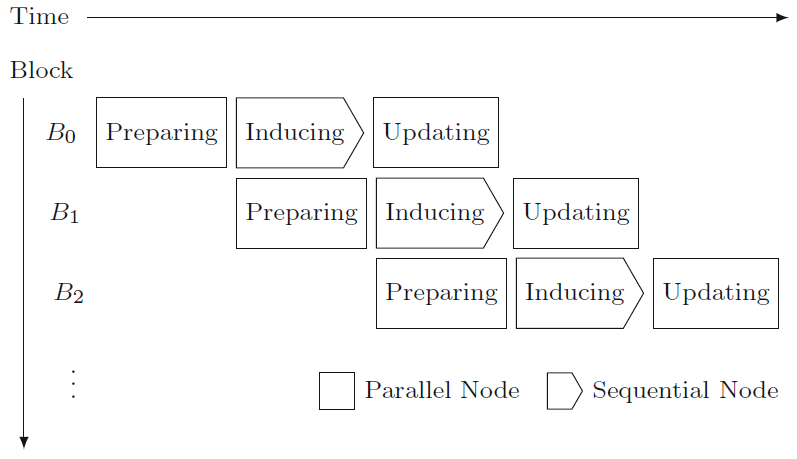
\includegraphics[width=\textwidth]{kapitel/saca_algorithmen/psais/psais_architecture.png}
\caption{Graphische Darstellung des verschränkten Induzierens in \cite{psais}}
\label{psaisArch}
\end{figure}


\subsection{Parallele Substring Benennung}

In \cite{psais} wird eine Methode gezeigt um das Benennen der LMS-Substrings vor dem Rekursionsaufruf zu parallelisieren. Dafür werden die geordneten Substrings in gleiche Blöcke zerteilt und für jeden Block wird ein Differenzen-Bitvektor berechnet. Für jeden Substring in dem Block, der verschieden von seinem nachfolgenden Substring ist, ist das zugeordnete Bit 1 in dem Vektor, andernfalls ist es 0. Aus den entstehenden Vektoren kann die Anzahl verschiedener Namen in diesem Block berechnet werden. Damit können die neuen Namen der jeweils ersten Substrings aller Blöcke sequentiell berechnet werden. Danach können parallel für jedem Block, ausgehend von dem bereits umbenannten ersten Substring des Blocks, die Namen der anderen Substrings des Blocks berechnet werden. \\

Diese Methode wurde in unserer Version des pSAIS aus Zeitmangel nicht implementiert. Die dort vorzufindende Art der Umbenennung erfolgt wie beim SAIS sequentiell.

\subsection{Paralleles Klassifizieren}\currentauthor{Christopher Poeplau}
\label{subsection:psais_classifying}

Um den SAIS auch beim initialen Klassifizieren zu beschleunigen, wird das Zuordnen von L- und S-Typen parallelisiert. Dabei wird der Text in Blöcke aufgeteilt, die selbständig von ihren Threads abgearbeitet werden. Um speichereffizient arbeiten zu können, werden die Typen in einen Bitvektor gespeichert. Das bedeutet die Threadgrenzen der Blöcke müssen immer einer Zweierpotenz entsprechen. Dies ist nötig, da die Datenstrukturen intern immer auf Bytes arbeiten und es beim Manipulieren der Bytes über Threadgrenzen hinweg zu \textit{Race-Conditions} kommen kann, das Ergebnis der Berechnung also davon abhängt, welcher Thread zuerst das jeweilige Byte bearbeitet.
Das parallele Klassifizieren funktioniert in zwei Durchgängen. 

Im ersten Durchgang klassifiziert jeder Thread seinen Block soweit es geht. Dabei ist es jedem Thread erlaubt, ein Zeichen über seinen eigenen Block zu schauen. Es ist ersichtlich, dass der letzte Thread, der den Block mit dem Sentinel bearbeitet, immer dazu in der Lage ist, seinen gesamten Block zu klassifizieren. Bei allen anderen Blöcken ist es möglich, dass sie kein oder nur einen Teil der Zeichen klassifizeren können. Jeder Thread speichert also zusätzlich bis zu welchem Zeichen er klassifizieren konnte. Falls er klassifizieren konnte, speichert er sich zusätzlich noch den klassifizierten Typ an der Threadgrenze, der für den zweiten Durchgang benötigt wird.
Exemplarisch für den ersten Durchgang folgt ein Beispiel. Der Einfachheit halber wurden die Threadgrenzen nach jeweils 4 Zeichen gesetzt und nicht byteweise:

\begin{center}
	\begin{tabular}{c|c|c|c}     
	           0     &             1         &           2          			&             3    \\   
          	aaaa     &          aaaa         &        aaba           			&          acc\$    \\            
         	xxxx     &          xxxx         &        SSLx           			&          SLLS     \\     
         	  x      &            x          &   \textcolor{blue}{S}            &          \textcolor{red}{S}      \\            	       
	\end{tabular}
\end{center}

Dadurch, dass das Sentinel das lexikographisch kleinstmögliche Zeichen ist und im pSAIS nur einmalig vorkommt, kann der 3. Block in seiner Gesamtheit klassifiziert werden. Der zweite Block versucht das letzte $a$ zu klassifizieren. Dies ist jedoch nicht möglich, da das nächste Zeichen auch ein $a$ ist. An dieser Stelle ist es noch nicht möglich, auf dessen Typ zuzugreifen und diesen zu übernehmen, da alle Threads gleichzeitig arbeiten und zu diesem Zeitpunkt nicht gewährleistet ist, dass der Typ schon geschrieben wurde. An den jeweiligen Stellen, die nicht klassifizert werden konnten steht ein $x$. Die Blöcke 0 und 1 konnten nichts klassifizieren, da auch mit dem nächsten Zeichen ihres Blocks keine Informationen über den Vorgängertypen ermitteln konnten. Alle Threads speichern zudem den ermittelten Typ an ihren Threadgrenzen. Da nur Block 2 und 3 klassifizieren konnten, steht nur bei ihnen kein $x$.

Im zweiten und finalen Durchgang des Klassifizierens werden die Informationen der benachbarten Blöcke genutzt, um den gesamten Text zu klassifizieren, der noch nicht klassifiziert werden konnte:

\begin{center}
	\begin{tabular}{c|c|c|c}      
		           0     	&             1         &           2           &             3    \\ 
          	aaaa     		&          aaaa         &        aaba           &          acc\$    \\            
\textbf{\textcolor{blue}{S}}\textbf{\textcolor{blue}{S}}\textbf{\textcolor{blue}{S}}\textbf{\textcolor{blue}{S}} &  \textbf{\textcolor{blue}{S}}\textbf{\textcolor{blue}{S}}\textbf{\textcolor{blue}{S}}\textbf{\textcolor{blue}{S}} & SSL\textbf{\textcolor{red}{S}}  & SLLS     \\             	       
	\end{tabular}
\end{center}

Im ersten Durchgang fehlte im Block 2 noch die Information, welchem Typ das $a$ entsprach. Diese Information ist nun vorhanden und das letzte Zeichen des Blocks kann klassifiziert werden. Analog verhält es sich mit den ersten beiden Blöcken, deren Zeichen alle S-Typen sind.



\newpage
\section{GSACA}

\subsection{Einleitung}
\label{gsaca:chapter1}
%
In \currentauthor{David Piper} diesem Abschnitt geht es um den Algorithmus GSACA. 
Grundlage hierf\�r bietet das Paper \textit{Linear-time Suffix Sorting - A New Approach for Suffix Array Construction} von Uwe Baier \cite{saca:3}. 
GSACA verfolgt bei der Konstruktion des Suffix Arrays einen neuen Ansatz und erstellt dieses in linearer Zeit ohne rekursiv zu arbeiten.
Eine vollst\�ndige Implementierung des Algorithmus l\�sst sich auf der GitHub-Seite \cite{saca:3:github} von Uwe Baier finden. \par
Zun\�chst wird in Kapitel \ref{gsaca:chapter2} das allgemeine Vorgehen des Algorithmus informell beschrieben. 
Kapitel \ref{gsaca:chapter3} wendet dies beispielhaft an dem Wort Banane an. 
Danach wird in Kapitel \ref{gsaca:chapter4} der Algorithmus vorgestellt und Zeile f\�r Zeile erkl\�rt. 
Anschlie\�end werden in Kapitel \ref{gsaca:chapter5} weitere Details der Implementierung besprochen.
Darauf folgt das Kapitel \ref{gsaca:chapter6} in dem GSACA auf die Eingabe \textit{caabaccaabacaa} angewendet wird, wie es zuvor auch schon bei anderen Algorithmen der Fall war.
Zum Schluss werden in Kapitel \ref{gsaca:chapter7} m\�gliche \�nderungen und Optimierungen besprochen. 

\newpage
\subsection{Das Vorgehen}
\label{gsaca:chapter2}
%
Bevor der konkrete Algorithmus pr{\"a}sentiert  wird, wird in diesem Kapitel das allgemeine Vorgehen beschrieben. Das Suffix Array f{\"u}r ein gegebenes Wort wird in zwei Phasen konstruiert.\\

Phase 1: Einteilung der Buchstaben in Gruppen und Bestimmung von sogenannten Gruppenkontexten f{\"u}r jede Gruppe. Ein Gruppenkontext ist ein Teilstring des originalen Wortes, so dass dieser Teilstring der Pr{\"a}fix eines Suffixes ist. Dieser Pr{\"a}fix umfasst den Beginn des Suffixes bis zu der Stelle, an der der Rest des Suffixes selbst ein Gruppenkontext ist. F{\"u}r das Wort Banane haben wir beispielsweise die beiden Suffixe Banane und anane. Wie im Beispiel zu sehen sein wird, ist der berechnete Gruppenkontext von anane anane selbst. Da der Gruppenkontext von Banane der Pr{\"a}fix bis zum n{\"a}chsten Gruppenkontext ist, und anane der Gruppenkontext von anane ist, ist der Gruppenkontext von Banane nur B. Zus{\"a}tzlich zu der Einteilung in Gruppen werden diese Gruppen lexikografisch nach ihren Gruppenkontexten sortiert. 
Am Anfang wird eine Tabelle mit den Buchstaben des Wortes, den Indices, den Kontexten und den Gruppen als Zeilen gebildet. Dann werden die initialen Gruppenkontexte aus den einzelnen Buchstaben des Wortes in lexikografischer Ordnung erstellt, beginnend mit dem Terminationssymbol \$. Die initialen Gruppen sind die Indices der Buchstaben des Gruppenkontextes im Wort. Anschlie{\ss}end werden f{\"u}r jede Gruppe in lexikographisch absteigender Reihenfolge die Buchstaben an den Indices dieser Gruppen im Wort betrachtet und deren direkte Vorg{\"a}ngergruppe im Wort bestimmt. Es wird ein \prevpointer, also ein Zeiger auf den Index des Vorg{\"a}ngers von dem gerade betrachteten Index, gespeichert und der Kontext der Vorg{\"a}ngergruppe um den gerade betrachteten Kontext erweitert. Bei dem Fall, dass nicht alle Buchstaben aus dieser Gruppe Vorg{\"a}nger der initial betrachteten Gruppe sind, sondern nur ein Teil von der Vorg{\"a}ngergruppe getroffen wurde, findet nur bei dem getroffenen Teil der Vorg{\"a}ngergruppe eine Kontexterweiterung statt. In diesem Fall muss die Vorg{\"a}ngergruppe aufgeteilt werden und eine neue Gruppe, bestehend aus der Teilgruppe mit erweitertem Kontext, wird direkt nach der Teilgruppe ohne Kontexterweiterung hinzugef{\"u}gt. \\

Phase 2: Die zuvor in Phase 1 berechnete Gruppenstruktur wird genutzt, um das finale Suffix Array zu erstellen. Hierzu werden die Gruppen in lexikografisch aufsteigender Reihenfolge durchlaufen.
Als erstes wird eine Tabelle gebildet mit den Buchstaben, den Indices, den Gruppen aus Phase 1 und den Startpositionen der Suffixe nach ihrer aktuellen Gruppe geordnet als Zeilen. Die Liste der Startpositionen SA ist zun{\"a}chst leer f{\"u}r alle Indices.
Danach wird SA[1] auf das Zeichen der ersten Gruppe (normalerweise das Terminationssymbol \$) gesetzt.
Anschlie{\ss}end wird {\"u}ber SA iteriert. Dazu wird in jedem Durchlauf das Zeichen des originalen Wortes an der Position, die in SA gespeichert ist, gesucht und das vorherige Zeichen betrachtet. Dann wird die Kette der \prevpointer ausgehend von diesem Zeichen durchlaufen, bis diese leer ist und die Indices der gefundenen Zeichen in SA gespeichert. 
\newpage
\subsection{Suffix Array Konstruktion am Beispiel Banane}
\label{gsaca:chapter3}
%
Nachdem im vorherigen Kapitel das Vorgehen beschrieben wurde, wird in diesem Kapitel das Suffix Array für das kurze Beispielwort Banane konstruiert.

\subsection*{Phase 1:}
In der ersten Phase werden die Gruppen und Gruppenkontexte für das Wort Banane erstellt. 
Dies geschieht in insgesamt vier Iterationen.\\

Iteration 1:\\
Schritt 1: Das Wort Banane besteht aus vier verschiedenen Buchstaben (a, b, e, n), zusammen mit dem Terminationssymbol \$ sind somit am Beginn der ersten Iteration fünf Gruppen vorhanden. 
In der in Tabelle \ref{fig_banane_1_1} dargestellten Tabelle sind in der oberen Hälfte die initialen Gruppen und Gruppenkontexte dargestellt und in der unteren Hälfte das Wort zusammen mit den Indices der Buchstaben. 
Der Algorithmus beginnt, indem der lexikographisch letzte Gruppenkontext betrachtet wird. 
In diesem Fall ist das der Buchstabe n, welcher an den Indices 3 und 5 in dem Wort vorkommt. 
Die entsprechenden Zellen der Tabelle sind grün hervorgehoben. \\
Schritt 2: Dann werden die Vorkommen der aktuell betrachteten Gruppe im Wort untersucht. 
In dieser ersten Iteration ist es das Vorkommen von dem Zei\-chen n an den Positionen 3 und 5. \\
Schritt 3: Danach werden die direkten Vorgänger im Wort untersucht. 
In diesem Schritt ist das der Buchstabe a an den Positionen 2 und 4. 
Diese Indices sind zusammen mit den Buchstaben an den entsprechenden Positionen in der Tabelle rot hinterlegt. \\
Schritt 4: Im letzten Schritt dieser Iteration wird der Gruppenkontext der im vorherigen Schritt markierten Buchstaben betrachtet und um den Kontext der initial in dieser Iteration betrachteten Gruppe erweitert. 
Da alle Vorkommen der Gruppe a Vorgänger von der Gruppe n waren, findet diese Kontexterweiterung bei allen Elementen statt. 
Somit wird aus der Gruppe a die Gruppe an. Das finale Ergebnis zeigt die Änderungen vor gelben Hintergrund an.\\

Iteration 2:\\
Schritt 1: In der zweiten Iteration, deren Schritte in Tabelle \ref{gsaca:fig_banane_1_2} verdeutlicht werden, wird die nächste Gruppe bezüglich der lexikographisch absteigenden Ordnung betrachtet. 
Dies ist die Gruppe mit Kontext e.\\
Schritt 2: Der Buchstabe e kommt nur an Index 6 im Wort vor.\\
Schritt 3: Für diesen Index wird die Vorgängergruppe gesucht. 
Diese ist die Gruppe an, die im vorherigen Schritt gebildet wurde.\\
Schritt 4: Anders als in der vorherigen Iteration werden in diesem Durchlauf nicht alle Vorkommen der Vorgängergruppe getroffen. 
Damit muss diese Gruppe in zwei neue Gruppen aufgeteilt werden. 
Der erste Teil der Gruppe bleibt an und der zweite Teil wird um den Kontext von e erweitert. 
Da die Gruppe mit dem erweiterten Kontext lexikographisch größer ist, wird sie zum neuen Nachfolger der Teilgruppe ohne Kontexterweiterung.\\

Iteration 3:\\
Schritt 1: Als nächstes wird die Gruppe b betrachtet. 
Die Zwischenergebnisse dieser Iteration sind in Tabelle \ref{fig_banane_1_3} zu sehen.\\
Schritt 2: Diese Gruppe hat keinen Vorgänger im betrachteten Wort. 
Daher endet diese Iteration ohne Änderungen an den Kontextgruppen.\\

Iteration 4: \\
Schritt 1: Es wird die nächste Gruppe betrachtet. Dies ist die Gruppe mit Kontext ane.\\
Schritt 2: Diese Gruppe umfasst die Indices 4 bis 6 im Wort Banane.\\
Schritt 3: Der Vorgänger dieser Gruppe ist die Gruppe an.\\
Schritt 4: Wie in der ersten Iteration wird die gesamte Vorgängergruppe getroffen. 
Diese wird um den Kontext der Gruppe ane erweitert. 
Das Ergebnis dieser Iteration und der gesamten Phase 1 ist in Tabelle \ref{fig_banane_1_4} gezeigt. 
Am Ende dieser Phase hat man somit 6 Gruppenkontexte: \$, anane, ane, b, e und n. 
Zusätzlich wurden für alle Buchstaben des Wortes die \prevpointer erzeugt und gespeichert. 
Die entstandenen Pointer-Ketten lassen sich in Abbildung \ref{fig_banane_prev_pointer} sehen. 
Auf diesem Ergebnis aufbauend wird in Phase 2 das finale Suffix Array berechnet werden.\\

\subsection*{Phase 2:}
In der zweiten Phase wird das Suffix Array mithilfe der zuvor erstellten Gruppen und Gruppenkontexte sowie der \prevpointer konstruiert. 
In diesem Beispiel werden hierfür 5 Iterationen durchlaufen.\\

Iteration 1:\\
Schritt 1: Die Phase 2 arbeitet auf einer anderen Tabelle als Phase 1. 
Die untere Hälfte der Tabelle enthält, genau wie die in Phase 1, das betrachtete Wort Banane und die Indices der Buchstaben. 
Die obere Hälfte besteht aus den Gruppen und Gruppenkontexten, wie sie aus Phase 1 übernommen wurden und aus der Liste SA. 
Diese enthält den Index des ersten Buchstaben des Suffixes.
Wie zuvor beschrieben werden in dieser Phase die Werte von SA von links nach rechts durchlaufen, beginnend mit der ersten Gruppe, in diesem Beispiel also mit der Gruppe \$ an Index 7. 
Die Tabelle und die einzelnen Schritte dieser Iteration sind in Tabelle \ref{fig_banane_2_1} gezeigt. 
Die aktuell betrachtete Gruppe ist durch grünen Hintergrund gekennzeichnet. \\
Schritt 2: Es wird das Zeichen \$ an Position 7 im Wort Banane betrachtet. 
Auch die aktuell bearbeitete Position ist durch grüne Farbe hervorgehoben. \\
Schritt 3: Um das nächste Element von SA zu bestimmen wird der direkte Vorgänger dieses Zeichens untersucht. 
Dabei bezieht sich diese Iteration also auf das Element 6, welches in der Zelle mit blauem Hintergrund zu sehen ist. \\
Schritt 4: Von diesem Element ausgehend werden die \prevpointer aus Phase 1 durchlaufen bis das letzte Element dieser Liste gefunden ist. 
Das Vorgängerelement von dem Zeichen e an Index 6, also das Zeichen, auf das der \prevpointer von e zeigt, ist das Zeichen a an Index 4. 
Dieses wiederum hat einen \prevpointer auf das Zeichen a an Index 2. Die betrachteten Indices, die in der Tabelle rot hinterlegt sind, werden in die Liste SA übertragen. 
Somit enthält diese am Ende der ersten Iteration drei weitere Indices, welche durch gelben Hintergrund hervorgehoben sind. \\

Iteration 2:\\
Schritt 1: In diesem Durchlauf wird das zweite Element in SA betrachtet, dies ist Index 2.\\
Schritt 2: Es wird dieser Index im Wort betrachtet.\\
Schritt 3: Der Vorgänger des Buchstaben a an Index 2 ist das Zeichen b an Index 1. 
Da b kein vorheriges Element hat, der \prevpointer also auf kein Element zeigt, endet diese Iteration hier. 
Der Index von Zeichen b wird in SA eingetragen. Das Ergebnis lässt sich in Tabelle \ref{fig_banane_2_2} sehen.\\

Iteration 3: \\
Schritt 1: Als nächstes wird das dritte Element von SA untersucht. 
Aus der Tabelle \ref{fig_banane_2_3} lässt sich erkennen, dass dies das Element an Index 4 ist.\\
Schritt 2: Das Zeichen an dem betrachteten Index ist a.\\
Schritt 3: Der Vorgänger von a an Index 4 ist n an Index 3.\\
Schritt 4: Der \prevpointer von n an Index 3 zeigt auf das a an Index 2. 
Der Index 2 ist bereits in SA enthalten, Index 3 aber noch nicht, daher wird dieser in die Liste aufgenommen.\\

Iteration 4: \\
Wie sich in der Tabellen \ref{fig_banane_2_4} sehen lässt, wird das Zeichen an Index 1 betrachtet. 
Dies ist das Zeichen b, welches kein Element hat, auf das sein \prevpointer zeigt. 
Somit endet diese Iteration ohne Änderung der Tabelle.\\

Iteration 5: \\
Schritt 1: In dieser Iteration wird das Element an Index 6 untersucht.\\
Schritt 2: Das Zeichen an Index 6 im Wort ist e.\\
Schritt 3: Es wird der Vorgänger von diesem Zeichen betrachtet. Die Tabelle zu dieser Iteration, Tabelle \ref{fig_banane_2_5}, zeigt, dass dies das Zeichen n an Index 5 ist.\\
Schritt 4: Dieses Zeichen hat einen Zeiger auf das Vorgängerelement a an Index 4. 
Wie in einer vorherigen Iteration hat dieses a einen Zeiger auf das Zeichen a an Index 2. 
Da die Zeichen an Index 4 und 2 bereits in der Liste SA enthalten sind, wird in diesem Schritt nur der Index 5 zu dieser Liste hinzugefügt. 
Somit ist die Liste vollständig gefüllt.\\

In diesem einfachen und kurzen Beispiel weicht die Liste der Gruppen, welche das Ergebnis von Phase 2 ist, nicht von der Liste SA ab.
Dies ist jedoch nicht immer der Fall, vor allem in längeren und komplexeren Beispielen unterscheiden sich diese teilweise. 
Diese Unterschiede werden bei der Berechnung des Suffix Arrays für das Wort \textit{caabaccaabacaa} in Kapitel \ref{gsaca:chapter6} deutlich. 
Je mehr Gruppen mit mehr als einem Index existieren, umso häufiger kann die Reihenfolge der Indices innerhalb dieser Gruppe gewechselt werden. 
Im Beispiel zum Wort Banane gab es jedoch nur eine Gruppe mit mehr als einem Index. 
In dieser Gruppe mit dem Buchstaben n fand keine Veränderung durch diese Schritte statt.\\

%%%%%%%%%%% Phase 1 %%%%%%%%%%%%%%%
\input{kapitel/saca_algorithmen/gsaca/tables/phase1-iteration1}
\input{kapitel/saca_algorithmen/gsaca/tables/phase1-iteration2}
\input{kapitel/saca_algorithmen/gsaca/tables/phase1-iteration3}
\input{kapitel/saca_algorithmen/gsaca/tables/phase1-iteration4}

\begin{figure}
	\begin{minipage}[H]{10cm}
		\centering
		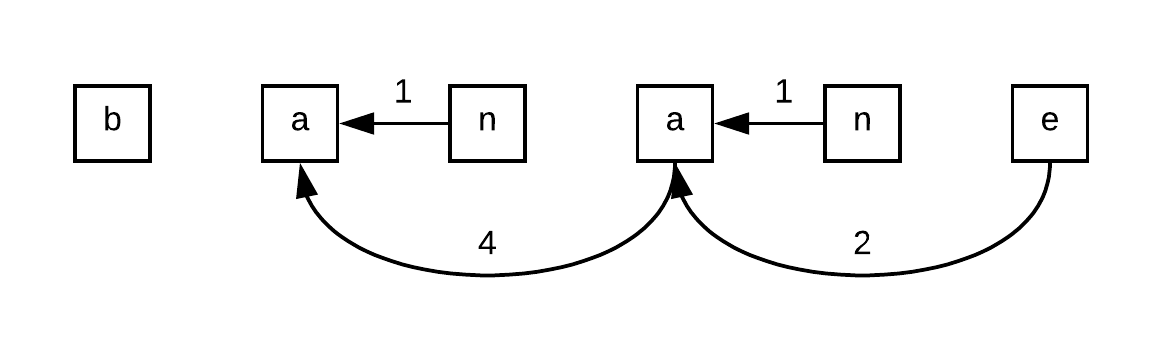
\includegraphics[width=10cm]{kapitel/saca_algorithmen/gsaca/images/Banane-prev-pointer}
	\end{minipage}
	\caption[Konstruktion des Suffix Arrays für das Wort Banane: \prevpointer]{Konstruktion des Suffix Arrays für das Wort Banane: \prevpointer. Die Zahlen geben die Nummer der Iteration an, in welcher der \prevpointer berechnet wurde.}
\label{fig_banane_prev_pointer}
\end{figure}

%%%%%%%%%%% Phase 2 %%%%%%%%%%%%%%%
\input{kapitel/saca_algorithmen/gsaca/tables/phase2-iteration1}
\input{kapitel/saca_algorithmen/gsaca/tables/phase2-iteration2}
\input{kapitel/saca_algorithmen/gsaca/tables/phase2-iteration3}
\input{kapitel/saca_algorithmen/gsaca/tables/phase2-iteration4}
\input{kapitel/saca_algorithmen/gsaca/tables/phase2-iteration5}

%%%%%%%%%%% Ergebnis %%%%%%%%%%%%%%%
%\input{kapitel/saca_algorithmen/gsaca/tables/results}
\newpage
\subsection{Der Algorithmus}
\label{gsaca:chapter4}
%
Nachdem zuvor das allgemeine Vorgehen beschrieben und an einem Beispiel verdeutlicht wurde, wird in diesem Kapitel der konkrete Algorithmus vorgestellt, wie er von Uwe Baier konzipiert wurde und in \ref{saca:3:code} zu sehen ist. 

In den ersten 12 Zeilen wird Phase 1 beschrieben. 
In den Zeilen 2 und 3 wird die initiale Einteilung in die lexikografisch sortierten Gruppen vorgenommen. 
In der for-Schleife, die die Zeilen 4 bis 12 umfasst, werden dann die Schritte für jede Gruppe durchlaufen, beginnend bei der lexikografisch größten. 
Die zweite for-Schleife in den Zeilen 5 und 6 bestimmt für jedes Element der gerade betrachteten Gruppe das direkt vorhergehende Zeichen im Wort und speichert einen \prevpointer auf dieses Zeichen. 
Gibt es kein vorheriges Zeichen, wird die 0 als \prevpointer gespeichert. 
Dies ermöglicht die Überprüfung, ob ein Zeichen ein vohergehendes Zeichen hat, indem der \prevpointer mit 0 verglichen wird. 
Dies geschieht in einer späteren Codezeile in Phase 2. 
Anschließend werden alle lexikografisch kleineren Gruppenkontexte, auf die ein \prevpointer eines Elements der gerade betrachteten Gruppe zeigt, in Untermengen geteilt. 
Diese Untermengen enthalten Elemente der lexikografisch kleineren Gruppen, auf die dieselbe Anzahl an \prevpointern zeigt.
Dies geschieht in den Zeilen 7 und 8. 
Anschließend beginnt in Zeile 9 eine weitere for-Schleife, die über alle Untermengen iteriert, die in den beiden vorherigen Zeilen erstellt wurden. 
Dabei wird jede Untermengen in Teilmengen unterteilt, die die gleichen Suffixe beinhalten. 
In einer letzten for-Schleife dieser Phase in den Zeilen 11 und 12 wird über jedes Element dieser Teilmengen iteriert. 
Dazu wird jedes Suffix dieser Teilmengen aus seiner ursprünglichen Gruppe entfernt und zu einer neuen Gruppe als direkter Nachfolger der alten Gruppe hinzugefügt.

Die Zeilen 13 bis 23 bilden die Schritte der Phase 2, in der das Suffix Array aus den zuvor gebildeten Gruppen konstruiert wird. 
In der Zeile 14 wird das letzte Zeichen des Wortes, also das Terminationssymbol \$, als erstes Element der Liste SA gespeichert. 
Anschließend werden in einer for-Schleife, die in Zeile 15 beginnt, die Indices von SA vom ersten Element bis zum letzten Element durchlaufen. 
In jeder Iteration dieser Schleife wird das Zeichen betrachtet, welches der direkte Vorgänger des Zeichens ist, welches in der Liste SA an der Position steht, die der Nummer der aktuellen Iteration entspricht. 
Dies geschieht in Zeile 16. Die nachfolgende while-Schleife aus Zeile 17 durchläuft die Liste der \prevpointer des im vorherigen Schritt bestimmten Zeichens. 
In dieser while-Schleife wird zunächst in Zeile 18 die Position des gerade betrachteten Zeichens bestimmt. 
Die Position ergibt sich aus der Kardinalität der Menge aller Suffixe in kleineren Gruppen, inkrementiert um 1. 
Anschließend wird überprüft, ob SA bereits ein Zeichen an diesem Index enthält. 
Falls dies der Fall ist, wurden dieses Zeichen und die Elemente der \prevpointer schon betrachtet und die aktuelle Iteration der for-Schleife wird abgebrochen. 
Gibt es jedoch noch kein Zeichen an dieser Stelle in der Liste SA, wird das aktuell betrachtete Zeichen dort gespeichert. 
Die Überprüfung, der gegebenenfalls erfolgende Abbruch der aktuellen Iteration und die neue Zuordnung erfolgen in den Zeilen 19 bis 21. 
In Zeile 22 wird dieses Zeichen dann aus seiner aktuellen Gruppe entfernt und in eine neue, direkt vor der alten Gruppe liegende Gruppe hinzugefügt.
Am Schluss der while-Schleife wird in Zeile 23 das Zeichen, auf den der \prevpointer des aktuellen Zeichens zeigt, zum betrachteten Element für die nächste Iteration der while-Schleife.\\

Im folgenden wird die erste Iteration der einzelnen Zeilen der zweiten Phase exemplarisch am Beispiel Banane durchlaufen:\\
14: 	SA[1] = 7\\
15:	for-Schleife wird mit $i$ = 1 begonnen\\
16:	$j$ = SA[$i$] - 1 = SA[1] - 1 = 6\\
17:	$j$ $\neq$ 0, in while-Schleife wird eingetreten\\
18:	$sr$ = |\{\$, anane, ane, b\}| = 4\\
19:	SA[$sr$ + 1] = nil, daher wird die 1. Iteration der for-Schleife nicht abgebrochen\\
21:	SA[$sr$ + 1] = $j$ = 6\\
22: 	$j$ wird aus der aktuellen Gruppe entfernt und in eine neue Gruppe eingefügt, die ein direkter Vorgänger der aktuellen Gruppe ist. Da $j$ das einzige Element dieser Gruppe ist, findet keine Änderung statt.\\
23:	$j$ = prev($j$) = 4. Die nächste Iteration der while-Schleife wird mit $j$ = 4 durchlaufen.

\input{kapitel/saca_algorithmen/gsaca/code/pseudocode}

\clearpage % add new page to move the next section down

\newpage
\subsection{Implementierung}
\label{gsaca:chapter5}
%
In diesem Kapitel werden einige Details für die Implementierung besprochen. \\

Wie Uwe Baier in seiner Abhandlung über GSACA beschreibt, werden für eine Umsetzung des Algorithmus insgesamt folgende sechs Arrays benötigt:\\
\sa enthält die nach der Reihenfolge der Gruppen sortierten Startpositionen der Suffixe. \\
\isa ist die inverse Permutation zum Array \sa. \\
\gsize speichert die Anzahl der Elemente jeder Gruppe. 
Diese wird am Anfang der Gruppe gespeichert und bis zur Ende mit Nullen aufgefüllt.\\
\glink enthält Zeiger von den Suffixen zu den ersten Elementen ihrer entsprechenden Gruppen. \\
\prev beinhaltet die in Phase 1 berechneten \prevpointer, die zu Beginn des Algorithmus alle mit nil initialisiert sind.\\
\pc zählt die \prevpointer von einer Gruppe zu einer anderen. 
Die Werte sind alle mit 0 initialisiert.\\
Die anfänglichen Werte der Arrays für das zuvor vorgestellte Beispiel Banane sind in Tabelle \ref{fig_datastructures} zu sehen.\\

\input{kapitel/saca_algorithmen/gsaca/tables/datastructures}

Der Autor beschreibt weiterhin, wie man diese Datenstrukturen nutzen kann, um verschiedene Aufgaben des Algorithmus effizient umzusetzen.\\

Das erste Problem, welches angesprochen wird, ist die initiale Sortierung der Gruppen nach absteigender lexikografischer Reihenfolge. 
Hierzu sei die Variable $gs$ der Startindex der aktuellen Gruppe und $ge$ der Endindex. 
Um nun zur nächsten Gruppe zu gelangen, wird der neue Endindex der nächsten Gruppe auf den direkten Vorgänger des Startindex der aktuellen Gruppe gesetzt, also ist $ge_{neu}$ = $gs$ - 1. 
Der neue Startindex $gs_{neu}$ kann bestimmt werden, indem zu dem neuen Endindex das Element aus dem Suffix-Array \sa gesucht und für dieses mit \glink der Zeiger auf das erste Element der Gruppe bestimmt wird. 
Somit ist $gs_{neu}$ = \glink[\sa[$gs - a$]]. 
Das Bestimmen der Gruppengrenzen der nächsten Gruppe geschieht in $\mathcal O(1)$ und die Iteration über alle Gruppen benötigt somit $\mathcal O(n)$ Zeit.\\

Als nächstes wird beschrieben, wie sich der \prevpointer für ein Element berechnen lässt. 
Der \prevpointer für ein Index kann bestimmt werden, indem der vorherige Index betrachtet wird. 
Von diesem neuen Index ausgehend wird die Kette der \prevpointer so lange verfolgt, bis ein Index gefunden ist, dessen zugehöriges Zeichen im Wort zu einer niedrigeren oder der gleichen Gruppe gehört wie die Gruppe des ursprünglich betrachteten Index. 
Ob eine Gruppe kleiner als eine andere Gruppe ist, kann über die Liste \glink überprüft werden. 
Falls der gefundene Index zu einer kleineren Gruppe gehört, wurde das Element, auf den der \prevpointer des Elements am ursprünglichen Index zeigt, gefunden. 
Falls der gefundene Index aber zur gleichen Gruppe gehört, wird dieses Verfahren mit diesem neuen Index als Ausgangspunkt durchgeführt. 
Auf das dann gefundene Element wird von den \prevpointern aller so in einem Schritt betrachteten Indices gezeigt. 
Dieses als \textit{pointer jumping} bekannte Verfahren benötigt $\mathcal O(n)$ Zeit.\\
Dieses Vorgehen kann am Beispiel aus Kapitel \ref{gsaca:chapter3} gezeigt werden. 
In Tabelle \ref{gsaca:fig_banane_1_2} ist die zweite Iteration der ersten Phase dargestellt. 
Zu Beginn der zweiten Iteration wurde die Gruppe \textit{n} schon betrachtet, in dieser Iteration wird also die Gruppe \textit{e} untersucht. 
Der entsprechende Index im Wort ist 6, daher wird der vorherige Index 5 betrachtet. 
Das Zeichen an diesem neuen Index ist \textit{n} und der \prevpointer zeigt auf das Zeichen \textit{a} an Index 4. 
Dieses Element gehört zu einer niedrigeren Gruppe, daher wurde der \prevpointer von Index 6 bestimmt.\\

Anschließend wird im Originalpaper das Problem behandelt, wie im nächsten Teil des Algorithmus die Gruppen und Teilgruppen erstellt werden können. 
Dies geschieht in zwei Schritten. 
Zunächst wird das Array \pc und dabei gleichzeitig das Set P erstellt. 
Dieser erste Schritt geschieht, indem alle Elemente des Wortes durchlaufen und deren \prevpointer betrachtet werden. 
Währenddessen wird für ein Element $i$ der Wert an \pc[\prev[$i$]] um 1 inkrementiert und falls \pc[\prev[$i$]] zuvor 0 war, wird \prev[$i$] in das Set P aufgenommen.\\
Für das Beispiel aus Kapitel \ref{gsaca:chapter3} funktioniert das folgendermaßen:\\
\prev[1] = 0\\
\prev[2] = 0\\
\prev[3] = 2 $\Rightarrow$ \pc[2] = 1 und P = P $\cup$ \{2\} = \{2\}\\
\prev[4] = 2 $\Rightarrow$ \pc[2] = 2\\
\prev[5] = 4 $\Rightarrow$ \pc[4] = 1 und P = P $\cup$ \{4\} = \{2, 4\}\\
\prev[6] = 4 $\Rightarrow$ \pc[4] = 2\\
\prev[7] = 0\\
In einem zweiten Schritt werden nun die Teilmengen von P gebildet, in denen auf jedes Element einer Teilmenge gleich oft von einem \prevpointer gezeigt wurde. 
Dazu wird das Set P durchlaufen, solange es nicht leer ist. 
In jeder Iteration wird für jedes Element aus P der Wert an der entsprechender Stelle in der Liste \pc um 1 dekrementiert. 
Wenn der Wert von \pc 0 wird, wird das Element aus dem Set P entfernt und zu einem neuen Set P\textsubscript{l} hinzugefügt, wobei der Subscript $l$ dem Index der Iteration entspricht. \\
Angewendet auf das Beispiel passiert folgendes:\\
Vor der 1. Iteration: \pc[2] = \pc[4] = 2\\
1. Iteration: \pc[2] = 1 und \pc[4] = 1 $\Rightarrow$ P\textsubscript{1} = \{\} \\
2. Iteration: \pc[2] = 0 und \pc[4] = 0 $\Rightarrow$ P\textsubscript{2} = \{2, 4\}\\

Danach geht der Autor darauf ein, wie die Suffixe neu angeordnet werden können. 
In der for-Schleife werden alle Teilmengen des Sets P durchlaufen, welche im vorherigen Schritt erstellt wurden. 
Um ein Element $p$ aus einer dieser Teilmengen zu entfernen, wird es zunächst mit dem letzten Element seiner Gruppe unter Hilfe von \sa und \isa getauscht. 
Das letzte Element der Gruppe von $p$ ist bestimmbar durch \glink[$p$] + \gsize[\glink[$p$]], da \glink auf das erste Element einer Gruppe zeigt und \gsize die Größe der Gruppe beinhaltet. 
Nun ist das Element $p$ das letzte Element seiner Gruppe. 
Indem der Wert in \gsize[\glink[$p$]] um 1 dekrementiert wird, wird das Element $p$ quasi aus seiner Gruppe entfernt. 
Im Anschluss muss \glink[$p$] auf \glink[$p$] + \gsize[\glink[$p$]] gesetzt werden, so dass es wieder auf den Beginn der neuen Gruppe zeigt. 
Abschließend wird auch die Größe der neuen Gruppe angepasst, indem \gsize[\glink[$p$]] erhöht wird.\\

Zum Schluss werden kurz verschiedene Einzelheiten zu Phase 2 erklärt. 
Es wird gesagt, dass der Wert $sr$, welcher die Anzahl der Suffixe aus niedrigeren Gruppen darstellt, aus \sa und \isa berechnet werden kann. 
Außerdem führt der Autor auf, dass die Überprüfung, ob ein Element bereits im Suffix-Array enthalten ist, durchgeführt werden kann, indem überprüft wird, ob die Liste \isa an dem Index den Wert 0 enthält. 
Um ein Element $j$ aus seiner aktuellen Gruppe zu entfernen und als direkten Nachfolger zu einer neuen Gruppe hinzuzufügen, wird zunächst der Wert von \sa[\isa[$j$]] in der Variable $sr$ gespeichert. 
Anschließend wird dieser Wert \sa[\isa[$j$]] inkrementiert, das Element $j$ in \sa[$sr$] gespeichert und \isa[$j$] auf 0 gesetzt. 
Dies führt dazu, dass die zuvor erwähnte Überprüfung feststellt, dass $j$ bereits in \sa enthalten ist.

\newpage
\subsection{Illustration des Algorithmus an einem komplexen Beispiel}
\label{gsaca:chapter6}

Nachfolgend wird der Algorithmus an dem Text \textit{caabaccaabacaa} als weiteres und komplexeres Beispiel demonstriert. 
Dabei werden auch die zuvor beschriebenen Datenstrukturen eingebunden. 
Wie zuvor werden die aktuellen Schritte und daraus resultierende Änderungen farblich hervorgehoben.
Allerdings werden die einzelnen Iterationen aufgrund des Umfangs dieses Beispiels nicht so detailliert beschrieben, wie in \ref{gsaca:chapter3}.
Zunächst zeigen die Tabellen \ref{table_complex_example_1_start} bis \ref{table_complex_example_1_10} schritt\-weise die Abläufe in Phase 1, in der die Gruppen gebildet und die Liste der \prevpointer aufgebaut wird. 
Anschließend werden in den Tabellen \ref{table_complex_example_2_start} bis \ref{table_complex_example_2_13} die einzelnen Iterationen zur Bildung des Suffix-Arrays in Phase 2 dargestellt.

\input{kapitel/saca_algorithmen/gsaca/tables/example_complex_phase1}
\input{kapitel/saca_algorithmen/gsaca/tables/example_complex_phase2}
\newpage
\subsection{Optimierungen}
\label{gsaca:chapter7}
% Einleitung / Ziel der Optimierung
Nachdem in den vorherigen Kapitel die Einzelheiten zu GSACA vorgestellt wurden, werden in diesem Kapitel Optimierungen und Änderungen am Algorithmus vorgestellt.
Dabei wurde das Augenmerk auf eine Reduktion des Speicherverbrauchs gelegt.
Ausgangspunkt war eine abgewandelte Implementierung des GSACA-Algorithmus, in dem die Liste GSIZE als Vektor gespeichert wurde.
Wie zuvor beschrieben, speichert GSIZE die Größen der Gruppen.
Dabei ist die eigentliche Größe lediglich am Startindex der Gruppe gespeichert, der Rest der Gruppeneinträge ist 0.
Hierdurch bot dieser Bestandteil des Algorithmus einen guten Einstiegspunkt, um den verbrauchten Speicherplatz zu verringern.
Die Idee zur Verbesserung, die verfolgt wurde, war, die Größe der einzelnen Elemente dieses Arrays zu reduzieren.
Ursprünglich wurden alle Elemente des Vektors als Integer gespeichert, so dass je nach Größe der Integer bis zu 64 Bit pro Eintrag benötigt wurden.
Durch geschickte Kodierung der Elemente gelang es, diese Größe auf zwei Bit pro Eintrag zu reduzieren. \par
% Beschreibung der Optimierung
Wie auch in der alten Version, wurden die Einträge in der neuen GSIZE-Liste mit geringerem Speicherverbrauch als Vektor gespeichert.
Jedoch wurden sie nicht als Integer sondern als boolsche Werte gespeichert.
Je zwei aufeinanderfolgende Bool-Werte kodieren dabei einen Eintrag in GSIZE, somit enthält der Vektor zwar doppelt so viele Einträge wie zuvor, aber jeder Eintrag belegt nur ein Bit.
Das erste Bit kennzeichnet den Start einer Gruppe.
Ist es auf true gesetzt, ist das entsprechende Element an dem Index das erste Element der Gruppe.
In der ursprünglichen Version enthielte dieser Index die Anzahl der Elemente der Gruppe.
Das zweite Bit markiert das Ende einer Gruppe.
Diese Information ist wichtig, da beim Umsortieren der Gruppenkontexte in Phase 1 von GSACA die hinteren Elemente der Gruppen abgespalten werden, ohne dass die Gruppengröße direkt aktualisiert wird.
Da die ursprüngliche Gruppengröße aber weiter verwendet wird, kann zu dem Zeitpunkt noch nicht das erste Element der Gruppe aktualisiert werden, es wird also gleichzeitig die alte Gruppengröße und die Größe der kleinen abgespaltenen Gruppen benötigt.
Wird nun die Größe einer Gruppe gespeichert, wird das erste Bit des ersten Elements der Gruppe auf 1 gesetzt.
Anschließend werden für alle weiteren Elemente der Gruppe sowohl das erste als auch das zweite Bit auf 0 gesetzt.
Schließlich wird das zweite Bit des letzten Elements der Gruppe auf 1 gesetzt.
Ein Beispiel für den Vergleich einer Gruppe mit der alten und der neuen Variante lässt sich in Tabelle \ref{compare_gsize_variants} sehen.
Das Lesen eines Wertes ist etwas komplexer als das Spei\-chern eines Wertes.
Wenn an der Index an einer beliebigen Stelle innerhalb einer Gruppe gelesen wird, ist das erste Bit 0, somit ist es nicht der Beginn der Gruppe.
Wie bei der ursprünglichen Variante wird als Gruppengröße 0 zurückgegeben.
Wird aber am Beginn einer Gruppe gelesen, ist also das erste Bit 1, muss die Größe der Gruppe erst bestimmt werden.
Hierzu wird der Vektor von dem abgefragten Index an durchlaufen, solange bis ein Element erreicht wird, dessen erstes Bit 1 ist, das also den Beginn der nächsten Gruppe darstellt.
Bei diesem Durchlauf wird die Anzahl der Elemente gezählt.
So kann aus der Struktur die Gruppengröße bestimmt werden. \par

\input{kapitel/saca_algorithmen/gsaca/tables/gsize_compare}

% Beschreibung des Ansatzes
Um diesen neuen Ansatz zu entwickeln, war es nötig, die Gleichheit der alten und der neuen Version nach jeder Operation sicherzustellen.
Hierzu wurde zunächst eine Klasse GSIZE\_LIST erstellt, welche die Verwaltung der alten Version kapselt.
Diese Klasse bot Methoden zum lesenden und schreibenden Zugriff auf die einzelnen Element und wurde anschließend in dem Algorithmus verwendet.
Dann wurde eine neue Klasse GSIZE\_BOOL hinzugefügt, welche die glei\-chen Methoden wie GSIZE\_LIST bereitstellte.
Hierdurch konnte innerhalb des Algorithmus an nur einer Stelle die verwendete Klasse ausgewechselt werden, indem statt einer Instanz von GSIZE\_LIST eine Instanz von GSIZE\_BOOL initialisiert wurde.
Jetzt konnte zwar die Implementierung einfach ausgetauscht werden, jedoch konnten die beiden Versionen noch nicht direkt miteinander verglichen werden.
Um dies zu tun wurde als drittes die Klasse GSIZE\_COMPARE erstellt.
Auch diese Klasse enthielt die gleichen Methoden wie GSIZE\_LIST und GSIZE\_BOOL und konnte so ohne große Änderungen vom Algorithmus verwendet werden.
GSIZE\_COMPARE verwaltet je eine Instanz der beiden anderen Klassen und leitet alle Operationen an beide weiter.
Verwendet GSACA nun eine Instanz dieser dritten Klasse und nutzt diese beispielsweise um einen Wert von GSIZE auszulesen, wird der Wert an dem abgefragten Index sowohl von GSIZE\_LIST als auch von GSIZE\_BOOL ausgelesen.
Auch beim Setzen eines neuen Wertes wendet GSIZE\_COMPARE diese Änderungen auf beide Implementierungen an.
Auf diese Art können in jedem Schritt die Werte von der alten und der neuen Variante verglichen werden.
Außerdem lässt sich bei Abweichungen direkt feststellen, in welchem Schritt es passiert ist, warum es gescheitert ist und, aufgrund der Richtigkeit von GSIZE\_LIST, welcher Wert eigentlich in GSIZE\_BOOL enthalten sein müsste.
Durch dieses Vorgehen konnte das Verhalten von GSIZE\_LIST auch in Grenzfällen passen analysiert und nachgebildet werden. \par
% Evaluation der Optimierung
Leider benötigt die neue Version GSIZE\_BOOL aber erheblich mehr Re\-chen\-auf\-wand, da sowohl beim Speichern eines neuen Wertes als auch beim Lesen eines Wertes die ursprüngliche Zahl berechnet werden muss.
Durch diesen Ansatz konnte der Speicherverbrauch im Vergleich zu der vorherigen Implementierung als Vektor reduziert werden.
Aufgrund der benötigten Umrechnung der Werte erhöhte sich jedoch die Laufzeit gegenüber dem vorherigen Ansatz deutlich.
Die Ergebnisse von Laufzeit- und Speicherverbrauchsmessungen auf Datensätzen verschiedener Größe lässt sich in \ref{compare_gsize_results} sehen.
Beide Varianten wurden drei mal ausgeführt, um Schwankungen auszugleichen.
Die gemessenen Werte beziehen sich dabei auf die Ausführungsdauer des Algorithmus und beziehen nicht die Initialisierungsphase oder das Einlesen und Vorbereiten der Texte mit ein.
Als Grundlage diente der Text \textit{english} des \textit{Pizza\&Chili Corpus} \cite{testdaten:pizzachilli2007}.
Wegen dieser starken Erhöhung der Laufzeit bei gleich\-zeitig nur relativ moderater Reduktion des Speicherverbrauchs ist der untersuchte Ansatz als keine sinnvolle Optimierung von GSACA anzusehen.
Jedoch hat sich der beschriebene Ansatz zum Vergleichen mehrerer alternativen Implementierungen als praktisch erwiesen.
Durch die parallele Ausführung mehrerer Varianten konnten schnell Abweichungen und Fehler gefunden werden.
Zusätz\-lich hatten die beiden Implementierungen von GSIZE nach jeder Operation den gleichen Zustand, so dass sich Unterschiede schnell untersuchen lassen konnten und der für die Ungleichheit verantwortlich Schritt reproduzierbar verglichen werden konnte. \par

\input{kapitel/saca_algorithmen/gsaca/tables/gsize_compare_results}

\newpage
% Nina 2018 - 2018
% RIP GOTO-SACA :'( </3
%\newcommand{\lms}{$suf_{LMS} $ }
\newcommand{\lmsx}{$suf_{LMSx} $ }
\newcommand{\lmsxnot}{$suf_{\overline{LMSx}} $ }
\newcommand{\lmsy}{$suf_{LMSy} $ }
\newcommand{\lmsynot}{$suf_{\overline{LMSy}} $ }
\newcommand{\lx}{$suf_{Lx} $ }
\newcommand{\lxnot}{$suf_{\overline{Lx}} $ }
\newcommand{\sx}{$suf_{Sx} $ }
\newcommand{\ly}{$suf_{Ly} $ }
\newcommand{\lynot}{$suf_{\overline{Ly}} $ }
\newcommand{\SAlms}{$SA_{LMS}$}
\newcommand{\SAs}{$SA_{S}$}
\newcommand{\SAl}{$SA_{L}$}
\newcommand{\SAlmsynotlmsx}{$SA_{suf_{\overline{LMSy}}\bigcap suf_{LMSx}}$ }
\newcommand{\SAlxlynot}{$SA_{suf_{Lx}\bigcap suf_{\overline{Ly}}}$ }
\newcommand{\SAlysx}{$SA_{suf_{Ly}\bigcup suf_{Sx}}$ }
\newcommand{\SAlsx}{$SA_{suf_{L}\bigcup suf_{Sx}}$ }
\newcommand{\SAlmsxnot}{$SA_{suf_{\overline{LMSx}}}$ }
\newcommand{\SAlmsynot}{$SA_{suf_{\overline{LMSy}}}$ }
\newcommand{\SAlx}{$SA_{suf_{Lx}}$}
\newcommand{\SAlxnot}{$SA_{suf_{\overline{Lx}}}$ }
\newcommand{\SAlynot}{$SA_{suf_{\overline{Ly}}}$ }
\newcommand{\SAsxnot}{$SA_{suf_{\overline{Sx}}}$ }


\section{goto-SACA}
Der \currentauthor{Janina Michaelis} Suffixarray Construction Algorithm von Keisuke Goto baut von der Idee her auf dem SAIS auf. Allerdings wird das Problem hier in O(n) Zeit und ohne Zusätzlichen Platzverbrauch gelöst. Im folgenden werden zunächst einige Begriffe erläutert, welche zum Verständnis des Algorithmus benötigt werden.
\subsection{Erläuterungen}
\paragraph{$\sigma$} Die Größe des Alphabets welches im String vorkommt.
\paragraph{LE[c]/RE[c]} Die linkeste (LE) bzw. rechteste (RE) Position in einem Buchstabenintervall im Suffixarray.
\paragraph{$CL_{c}$/$CR_{c}$} Die Anzahl der L- bzw. S-Suffixe, welche mit c starten. 
\paragraph{LMSx} Pro Buchstaben das kleinste LMS-Suffix.
\paragraph{LMSy} Pro Buchstaben, für den es kein L Suffix gibt, das kleinste LMS-Suffix.
\paragraph{Lx} Pro Buchstaben das größte L-Suffix. 
\paragraph{Ly} Pro Buchstabe, für den kein S-Suffix existiert, das größte L-Suffix.
\paragraph{Sx} Pro Buchstabe das kleinste S-Suffix.
\paragraph{SA} Das Suffix-Array.
\paragraph{T} Der String, für welchen das Suffix-Array gesucht wird.
\paragraph{$T_{i}$} Das Suffix ab dem Index i.
\bigskip
Es gilt du beachten, dass der Algorithmus von Goto auf Integeralphabete ausgelegt ist. Deshalb muss der String vor Start des Algorithmus falls notwendig in Integerzahlen umgewandelt werden.

\subsection{LMS-Substring Sortierung}
Im ersten Schritt des Algorithmus werden die LMS-Substrings sortiert. Hierfür werden zunächst zwei separate Hilfsarray Y und Z benötigt. Diese sind Subarrays von A. Z nimmt die letzten | \lmsxnot| Zeichen von A ein und Y die |$\sigma$ | Zeichen davor. Im ersten Schritt werden alle LMS-Substrings nach Anfangsbuchstaben sortiert in A gespeichert. Dafür wird zunächst RE bezüglich \lmsxnot für jeden Buchstaben in Y gespeichert. Also RE[c] in Y[c]. Dann wird T von rechts nach links durchlaufen und jeder LMS-Substring $T'_{i}$ wird in Z[RE[$c_{i}$]] gespeichert. Hierbei kann es vorkommen, dass der Platz in Z schon belegt ist. Dann werden die zwei Substrings verglichen und der größere in Z gespeichert. Der kleinere wird in Y[$c_{i}$] abgelegt. Wenn T durchlaufen ist, sind alle LMS-Substrings in Y und Z gespeichert. Da in Y Lücken seien können, werden alle darin gespeicherten Substrings ans Ende von Y, in $Y_{1}$ der Länge | \lmsx | geschoben. Im Anschluss werden $y_{1}$ und Z über die Anfangsbuchstaben der Substrings gemergt. In den letzten | \lms | Einträgen von A sind nun die nach Anfangsbuchstaben sortierten LMS-Substrings gespeichert. \\
Nun müssen die Substrings lexikografisch sortiert werden. Es wird in drei Schritten vorgegangen:
\paragraph{Schritt 1:}
Die LMS-Substrings werden von links nach rechts durchlaufen und jeder gelesene Substring $T_{i}$ wird in $A[RE[c_{i}]]$ verschoben und $RE[c_{i}]$ um eins verringert.
\paragraph{Schritt 2:}
Von links nach rechts werden alle Substrings in A gelesen. Bei jedem Substring $T'_{i}$ wird sein Vorgänger $T_{i-1}$ betrachtet. Wenn dieser ein L-Substring ist, wird er in $A[LE[c_{i-1}]]$ gespeichert und LE[$c_{i-1}$] inkrementiert. Nachdem $T'_{i}$ gelesen wurde, wird er aus A gelöscht.
\paragraph{Schritt 3:}
Von rechts nach links werden alle Substrings in A gelesen. Bei jedem Substring $T'_{i}$ wird sein Vorgänger $T_{i-1}$ betrachtet. Wenn dieser ein S-Substring ist, wird er in $A[RE[c_{i-1}]]$ gespeichert und RE[$c_{i-1}$] dekrementiert. Nachdem $T'_{i}$ gelesen wurde, wird er aus A gelöscht.
\bigskip
Nun liegen alle LMS-Substrings in sortierter Reihenfolge vor und können wieder an das Ende von A verschoben werden.
\subsection{LMS-Suffix Sortierung}
Sollten alle LMS-Substrings einzigartig sein, können die LMS-Suffixe einfach von diese adaptiert werden.
Anderenfalls wird ein String $T^{1}$ erstellt, in welchem jeder LMS-Substring in T durch seinen Rang unter den sortierten LMS-Substrings ersetzt wird. Um die richtige Reihenfolge der LMS-Substrings wird das Suffixarray von $T^{1}$ berechnet.
\subsection{L-Suffix Sortierung}
Nachdem die LMS-Suffixe sortiert vorliegen, werden darauf aufbauend die L-Suffixe sortiert. Dieser Schritt wird in neun Transitionen unterteilt.
\paragraph{Transition 1}
Alle sortierten LMS-Suffixe werden an das Ende von A, also in das Subarray Z verschoben.
\paragraph{Transition 2}
Das Ziel von Transition 2 soll es sein das Suffix-Array für \lmsxnot  im Subarray Z2 zu speichern und die unsortierten \lmsx  in Z1 abzulegen.\\
Dafür werden die sortierten LMS-Suffixe von rechts nach links durchlaufen und falls \SAlms [i] $\in$ \lmsxnot , wird es mit Z2[j] getauscht. j startet bei |Z2| und wird bei jedem Tausch dekrementiert.
\paragraph{Transition 3}
Die \lmsx in Z1 = $T_{j}$ werden von links nach rechts in Y[$c_{j}$] verschoben.
\paragraph{Transition 4}
Ziel dieser Transition ist es die \lmsy in Y zu speichern und das \SAlmsynotlmsx zwischen Y und Z2 abzulegen.\\
Dafür werden zunächst die Typen in Y festgelegt. Initial werden diese alle auf S gesetzt. Bei einem Scan von rechts nach links über T wird der Typ  von jedem Y[$c_{i}$] auf L gesetzt, wenn $T_{i}$ ein L-Suffix ist. Im   Anschluss wird jeder Eintrag von Y der vom Typ L ist von rechts nach    links in Z1 verschoben.
\paragraph{Transition 5}
\SAlmsynotlmsx in Z1 und \SAlmsxnot in Z2 werden über die Anfangsbuchstaben der Suffixe gemergt und man erhält \SAlmsynot in Z3.
\paragraph{Transition 6}
Jeder Eintrag in Y, welcher vom Typ L ist, wird auf 0 gesetzt. Dann wird für jedes c die Anzahl der L-Suffixe in Y[c] gespeichert, welche mit c beginnen. Anschließend wird von recht nach links auf Y jeder  Eintrag vom Typ L wie folgt neu berechnet: $\sum_{c'<c} max(0, CL_{c'}-1)$. Dadurch entsteht LE[c] in Y.
\paragraph{Transition 7}
Hier wird jeweils in drei Schritten vorgegangen.
\subparagraph{Schritt 1: Lese alle L- und LMS-Suffixe in lexikogr. Reihenfolge}
Suffixe die in X1, Y und Z3 gespeichert sind, sind darin sortiert. Jeweils von links nach rechts werden die drei Subarrays gelesen und das kleinste Suffix ausgewählt. Der entsprechende Iterator $i_{x}$, $i_{y}$ oder $i_{z}$ wird inkrementiert.\\
X1 enthält entweder ein L-Suffix oder ist leer.\\
Y enthält entweder ein Suffix aus \lx $\bigcup$ \lmsy, einen Wert für LE oder ist leer.\\
Z3 enthält ein LMS-Suffix.\\
Wenn ein Iterator größer wird als sein entsprechendes Array erhält er den Wert $\sigma + 1$, so dass dieser Eintrag auf keinen Fall mehr gewählt wird. Ist ein Eintrag in X1 leer, erhält er ebenfalls dem Wert $\sigma + 1$. Enthalten alle drei gelesenen Einträge den gleichen Wert, gilt X1<Y<Z3. Es könnte das Problem aufkommen, dass Y gelesen wird, aber kein Suffix sondern einen Wert für LE[$c_{i}$] enthält, oder leer ist. Dieses Problem wird wie folgt gelöst:\\
Wenn Y leer ist, impliziert das, dass kein L- oder LMS-Suffix mit dem entsprechenden Anfangsbuchstaben existiert. $i_{y}$ wird einfach inkrementiert und das kleinste Suffix wird erneut gesucht. Wie wird erkannt, ob Y einen Wert für LE enthält? Im Normalfall enthält Y für jeden Buchstaben das größte L-Suffix. Ist dies nicht der Fall, enthält es noch den Wert für LE und das entsprechende Suffix aus \lx wurde zuvor aus X1 gelesen. Wenn man also das zuletzt gelesene Suffix und das dazugehörige Array speichert, weiß man, dass wenn ein Suffix mit gleichem Startbuchstaben $i_{y}$ aus X1 gelesen wurde, Y einen Wert für LE enthält. Für diesen Fall wird $T_{j}$ = X1[$i_{x}-1$] in LE[$i_{y}$] verschoben und $i_{y}$ inkrementiert. $i_{x}$ wird dekrementiert.
\subparagraph{Schritt 2: Entscheide, ob $T_{i-1}$ ein L-Suffix ist}
Wenn $T_{i}$ auf X1 oder Z3 gelsen wird, kennen wir dessen Typ und können den Typ von $T_{i-1}$ durch Vergleichen der Anfangsbuchstaben in Erfahrung bringen. Wenn $T_{i}$ aus Y gelesen wird, wissen wir das $c_{i}\neq c_{i-1}$. Also können diese beiden einfach verglichen werden, um den Typ zu bestimmen
\subparagraph{Schritt 3: Speichere $T_{i-1}$, wenn es ein L-Suffix ist}
Wenn $X1[LE[c_{i-1}]]$ leer ist, wird $T_{i-1}$ darin gespeichert und $LE[c_{i-1}]$ inkrementiert. Anderenfalls besteht ein Konflikt zwischen $T_{i-1}$ und $T_{j}$ gespeichert in $X1[LE[c_{i-1}]]$. Vergleiche beide Anfangsbuchstaben, speichere das größere von beiden in $X1[LE[c_{i-1}]]$ und das kleinere in $Y[min(c_{i-1},c_{j}]$. Wenn $c_{i-1}>c_{j}$, inkrementiere $LE[c_{i-1}]$ und $i_{y}$.
\bigskip
Jedes in Schritt 1 gelesene Suffix durchläuft erst Schritt 2 und 3, bevor das nächste Suffix gelesen wird. Abschließend erhalten wir \SAlxnot in X1 und $LE_{suf_{Lx}\bigcup suf_{LMSy}}$ in Y.
\paragraph{Transition 8}
In dieser Transition soll \SAlx in X2 erstellt werden.\\
Verschiebe dafür von links nach rechts jeden Eintrag vom Typ L aus Y nach X2. Im Anschluss wird jeder Eintrag außerhalb von X gelöscht.
\paragraph{Transition 9}
\SAlx in X1 und \SAlxnot in X2 werden über die Anfangsbuchstaben der Suffixe zu \SAl in X gemergt.
\bigskip
Nach diesen 9 Schritte liegt das sortierte Suffix-Array der L-Suffixe am Anfang von A.
\subsection{S-Suffix Sortierung}
Das Prinzip beim Sortieren der S-Suffixe ist das gleiche wie beim Sortieren der L-Suffixe. Die Subarray Aufteilung ist ein wenig anders und die Schritte müssen geringfügig angepasst werden.
\paragraph{Transition 1}
entfällt
\paragraph{Transition 2}
Das Ziel von Transition 2 soll es sein das Suffix-Array für \lxnot  im Subarray X1 zu speichern und die unsortierten \lx  in X2 abzulegen.\\
Dafür werden die sortierten L-Suffixe von links nach rechts durchlaufen und falls \SAl [i] $\in$ \lxnot , wird es mit X1[j] getauscht. j startet bei 0 und wird bei jedem Tausch inkrementiert.
\paragraph{Transition 3}
Die \lx in X2 = $T_{j}$ werden von rechts nach links in Y[$c_{j}$] verschoben.
\paragraph{Transition 4}
Ziel dieser Transition ist es die \ly in Y zu speichern und das \SAlxlynot zwischen Y und X1 abzulegen.\\
Dafür werden zunächst die Typen in Y festgelegt. Initial werden diese alle auf L gesetzt. Bei einem Scan von rechts nach links über T wird der Typ  von jedem Y[$c_{i}$] auf S gesetzt, wenn $T_{i}$ ein S-Suffix ist. Im   Anschluss wird jeder Eintrag von Y der vom Typ S ist von links nach    rechts in X2 verschoben.
\paragraph{Transition 5}
\SAlxlynot in X2 und \SAlxnot in X1 werden über die Anfangsbuchstaben der Suffixe gemergt und man erhält \SAlynot in X3.
\paragraph{Transition 6}
Jeder Eintrag in Y, welcher vom Typ S ist, wird auf 0 gesetzt. Dann wird für jedes c die Anzahl der S-Suffixe in Y[c] gespeichert, welche mit c beginnen. Anschließend wird von links nach rechts auf Y jeder Eintrag vom Typ S wie folgt neu berechnet: $\sum_{c'\leq c} max(0, CS_{c'}-1)$. Sollte im Anschluss der Wert >0 sein, wird noch ein mal -1 gerechnet. Dadurch entsteht RE[c] in Y.
\paragraph{Transition 7}
Auch hier wird wieder jeweils in drei Schritten vorgegangen.
\subparagraph{Schritt 1: Lese alle S- und LMS-Suffixe in lexikogr. Reihenfolge}
Suffixe die in X3, Y und Z gespeichert sind, sind darin sortiert. Jeweils von rechts nach links werden die drei Subarrays gelesen und das größte Suffix ausgewählt. Der entsprechende Iterator $i_{x}$, $i_{y}$ oder $i_{z}$ wird dekrementiert.\\
X3 enthält ein L-Suffix.\\
Y enthält entweder ein Suffix aus \sx $\bigcup$ \ly, einen Wert für RE oder ist leer.\\
Z enthält entweder ein S-Suffix oder ist leer.\\
Wenn ein Iterator kleiner wird als Null erhält er den Wert -1, so dass dieser Eintrag auf keinen Fall mehr gewählt wird. Ist ein Eintrag in Z leer, erhält er ebenfalls dem Wert -1. Enthalten alle drei gelesenen Einträge den gleichen Wert, gilt X3<Y<Z. Es könnte das Problem aufkommen, dass Y gelesen wird, aber kein Suffix sondern einen Wert für RE[$c_{i}$] enthält, oder leer ist. Dieses Problem wird wie folgt gelöst:\\
Wenn Y leer ist, impliziert das, dass kein L- oder LMS-Suffix mit dem entsprechenden Anfangsbuchstaben existiert. $i_{y}$ wird einfach dekrementiert und das größte Suffix wird erneut gesucht. Wie wird erkannt, ob Y einen Wert für RE enthält? Im Normalfall enthält Y für jeden Buchstaben das größte S-Suffix. Ist dies nicht der Fall, enthält es noch den Wert für RE und das entsprechende Suffix aus \sx wurde zuvor aus Z gelesen. Wenn man also das zuletzt gelesene Suffix und das dazugehörige Array speichert, weiß man, dass wenn ein Suffix mit gleichem Startbuchstaben $i_{y}$ aus Z gelesen wurde, Y einen Wert für RE enthält. Für diesen Fall wird $T_{j}$ = Z[$i_{x}+1$] in RE[$i_{y}$] verschoben und $i_{y}$ dekrementiert.
\subparagraph{Schritt 2: Entscheide, ob $T_{i-1}$ ein S-Suffix ist}
Wenn $T_{i}$ auf X3 oder Z gelesen wird, kennen wir dessen Typ und können den Typ von $T_{i-1}$ durch Vergleichen der Anfangsbuchstaben in Erfahrung bringen. Wenn $T_{i}$ aus Y gelesen wird, wissen wir das $c_{i}\neq c_{i-1}$. Also können diese beiden einfach verglichen werden, um den Typ zu bestimmen
\subparagraph{Schritt 3: Speichere $T_{i-1}$, wenn es ein S-Suffix ist}
Wenn $Z[RE[c_{i-1}]]$ leer ist, wird $T_{i-1}$ darin gespeichert und $RE[c_{i-1}]$ dekrementiert. Anderenfalls besteht ein Konflikt zwischen $T_{i-1}$ und $T_{j}$ gespeichert in $Z[RE[c_{i-1}]]$. Vergleiche beide Anfangsbuchstaben, speichere das größere von beiden in $Z[RE[c_{i-1}]]$ und das kleinere in $Y[min(c_{i-1},c_{j}]$. Wenn $c_{i-1}>c_{j}$, dekrementiere $RE[c_{i-1}]$.
\bigskip
Jedes in Schritt 1 gelesene Suffix durchläuft erst Schritt 2 und 3, bevor das nächste Suffix gelesen wird. Abschließend erhalten wir \SAsxnot in X3 und $RE_{suf_{Sx}\bigcup suf_{Ly}}$ in Y.
\paragraph{Transition 8}
\SAlysx in Y und \SAlynot in X3 werden über die Anfangsbuchstaben der Suffixe gemergt und man erhält \SAlsx in X3+Y.
\paragraph{Transition 9}
\SAlsx in X3Y und \SAsxnot in Z werden über die Anfangsbuchstaben der Suffixe gemergt und man erhält SA in A.
\bigskip
Somit erhält man das vollständige Suffix-Array von T.
\subsection{Beispiel}
Im folgenden wird der Algorithmus an einem Beispielstring "caabaccaabacaa" verdeutlicht.
\begin{center}
    \begin{tabular}{ | l | c | c | c | c | c | c | c | c | c | c | c | c | c | c | c | c | }
        \hline
        $i$ & 0 & 1 & 2 & 3 & 4 & 5 & 6 & 7 & 8 & 9 & 10 & 11 & 12 & 13 & 14 \\ \hline
        $T$ & c & a & a & b & a & c & c & a & a & b & a & c & a & a & \$ \\ \hline
        $type$ & L & S & S & L & S & L & L & S & S & L & S & L & L & L & S \\ 
        \hline
    \end{tabular}
\end{center}
\textbf{LMSx:} 7, 14\\
\textbf{$\overline{LMSx}$:} 1, 4, 10\\
\textbf{LMSy:} 14\\
\textbf{$\overline{LMSy}$:} 1, 4, 7, 10\\
\textbf{Lx:} 3, 5, 12\\
\textbf{$\overline{Lx}$:} 0, 6, 9, 11, 13\\
\paragraph{LMS-Substring Sortierung}
\begin{center}
    \resizebox{\textwidth}{!}{
        \begin{tabular}{ | l | c | c | c | c | c | c | c | c | c | c | c | c | c | c | c | c | }
            \hline
            $i$ & 0 & 1 & 2 & 3 & 4 & 5 & 6 & 7 & 8 & 9 & 10 & 11 & 12 & 13 & 14 \\ \hline
            $T$ & c & a & a & b & a & c & c & a & a & b & a & c & a & a & \$ \\ \hline
            $T$ & 3 & 1 & 1 & 2 & 1 & 3 & 3 & 1 & 1 & 2 & 1 & 3 & 1 & 1 & 0 \\ \hline
            $type$ & L & S & S & L & S & L & L & S & S & L & S & L & L & L & S \\ 
            \hline
            \hline
            $A$ & & & & & & & & & & & & & & & \\ \hline
            & \multicolumn{8}{c|}{} & \multicolumn{4}{c|}{Y} & \multicolumn{3}{c|}{Z}\\ \hline
            $A$ & & & & & & & & & & 2 & & & & & \\ \hline
            $A$ & & & & & & & & & & 2 & & & 14' & & \\ \hline
            & \multicolumn{8}{c|}{} & \multicolumn{4}{c|}{Y} & \multicolumn{3}{c|}{Z}\\ \hline
            $A$ & & & & & & & & & & 1 & & & 14' & & 10'\\ \hline
            $A$ & & & & & & & & & & 0 & & & 14' & 7' & 10' \\ \hline
            & \multicolumn{8}{c|}{} & \multicolumn{4}{c|}{Y} & \multicolumn{3}{c|}{Z}\\ \hline
            $A$ & & & & & & & & & 14' & & & & 4' & 7' & 10' \\ \hline
            $A$ & & & & & & & & & 14' & 1' & & & 4' & 7' & 10' \\ \hline
            & \multicolumn{8}{c|}{} & \multicolumn{4}{c|}{Y} & \multicolumn{3}{c|}{Z}\\ \hline
            $A$ & & & & & & & & & & & 14' & 1' & 4' & 7' & 10' \\ \hline
            & \multicolumn{10}{c|}{} & \multicolumn{2}{c|}{Y1} & \multicolumn{3}{c|}{Z}\\ \hline \hline
            $A$ & & & & & & & & & & & 14' & 1' & 4' & 7' & 10' \\ \hline
            $A$ & 14' & & & & 10' & 7' & 4' & 1' & & & & & & & \\ \hline \hline
            $A$ & 14' & 13' & & & 10' & 7' & 4' & 1' & & & & & & & \\ \hline
            $A$ & & 13' & & & 10' & 7' & 4' & 1' & & & & & & & \\ \hline 
            $A$ & & 13' & 12' & & 10' & 7' & 4' & 1' & & & & & & & \\ \hline
            $A$ & & & 12' & & 10' & 7' & 4' & 1' & & & & & & & \\ \hline
            $A$ & & & 12' & & 10' & 7' & 4' & 1' & & & 11' & & & & \\ \hline
            $A$ & & & & & 10' & 7' & 4' & 1' & & & 11' & & & & \\ \hline
            $A$ & & & & & 10' & 7' & 4' & 1' & 9' & & 11' & & & & \\ \hline
            $A$ & & & & & & 7' & 4' & 1' & 9' & & 11' & & & & \\ \hline
            $A$ & & & & & & 7' & 4' & 1' & 9' & & 11' & 6' & & & \\ \hline
            $A$ & & & & & & & 4' & 1' & 9' & & 11' & 6' & & & \\ \hline
            $A$ & & & & & & & 4' & 1' & 9' & 3' & 11' & 6' & & & \\ \hline
            $A$ & & & & & & & & 1' & 9' & 3' & 11' & 6' & & & \\ \hline
            $A$ & & & & & & & & 1' & 9' & 3' & 11' & 6' & 0' & & \\ \hline
            $A$ & & & & & & & & & 9' & 3' & 11' & 6' & 0' & & \\ \hline
            $A$ & & & & & & & & & 9' & 3' & 11' & 6' & 0' & & \\ \hline
            $A$ & & & & & & & & & 9' & 3' & 11' & 6' & 0' & 5' &\\ \hline
            $A$ & & & & & & & & & 9' & 3' & 11' & & 0' & 5' & \\ \hline \hline
            $A$ & & & & & & & & & 9' & 3' & 11' & & 0' & 5'  &\\ \hline
            $A$ & & & & & & & & 4' & 9' & 3' & 11' & & 0' & 5' & \\ \hline
            $A$ & & & & & & & & 4' & 9' & 3' & 11' & & 0' & &  \\ \hline
            $A$ & 14' & & & & & & & 4' & 9' & 3' & 11' & & 0' & & \\ \hline
            $A$ & 14' & & & & & & & 4' & 9' & 3' & 11' & & & & \\ \hline
            $A$ & 14' & & & & & & 10' & 4' & 9' & 3' & 11' & & & & \\ \hline
            $A$ & 14' & & & & & & 10' & 4' & 9' & 3' & & & & & \\ \hline
            $A$ & 14' & & & & & 2' & 10' & 4' & 9' & 3' & & & & & \\ \hline
            $A$ & 14' & & & & & 2' & 10' & 4' & 9' & & & & & & \\ \hline
            $A$ & 14' & & & & 8' & 2' & 10' & 4' & 9' & & & & & & \\ \hline
            $A$ & 14' & & & & 8' & 2' & 10' & 4' & & & & & & & \\ \hline
            $A$ & 14' & & & 1' & 8' & 2' & 10' & 4' & & & & & & & \\ \hline
            $A$ & 14' & & & 1' & 8' & & 10' & 4' & & & & & & & \\ \hline
            $A$ & 14' & & 7' & 1' & 8' & & 10' & 4' & & & & & & & \\ \hline
            $A$ & 14' & & 7' & 1' & & & 10' & 4' & & & & & &  &  \\ \hline
            $A$  & & & & & & & & & & & 14' & 7' & 1' & 10' & 4' \\ \hline
        \end{tabular}
    }
\end{center}
Da alle LMS-Substrings einzigartig sin, können die LMS-Suffixe übernommen werden. Es kann mit dem nächsten Schritt fortgefahren werden.
\paragraph{L-Suffix Sortierung}
\begin{center}
    \resizebox{\textwidth}{!}{
        \begin{tabular}{ | l | c | c | c | c | c | c | c | c | c | c | c | c | c | c | c | c | }
            \hline
            $i$ & 0 & 1 & 2 & 3 & 4 & 5 & 6 & 7 & 8 & 9 & 10 & 11 & 12 & 13 & 14 \\ \hline
            $T$ & c & a & a & b & a & c & c & a & a & b & a & c & a & a & \$ \\ \hline
            $T$ & 3 & 1 & 1 & 2 & 1 & 3 & 3 & 1 & 1 & 2 & 1 & 3 & 1 & 1 & 0 \\ \hline
            & \multicolumn{5}{c|}{X1} & \multicolumn{3}{c|}{X2} & & & \multicolumn{2}{c|}{Z1} & \multicolumn{3}{c|}{Z2}\\ \hline
            & & & & & & & & \multicolumn{4}{c|}{Y} & \multicolumn{4}{c|}{Z3} \\ \hline
            $A$  & & & & & & & & & & & 14 & 7 & 1 & 10 & 4 \\ \hline
            \multicolumn{16}{c}{\textbf{Transition 1}}\\
            \hline
            $A$  & & & & & & & & & & & 14 & 7 & 1 & 10 & 4 \\ \hline
            \multicolumn{16}{c}{\textbf{Transition 2}}\\
            \hline
            $A$  & & & & & & & & & & & 14 & 7 & 1 & 10 & 4 \\ \hline
            \multicolumn{16}{c}{\textbf{Transition 3}}\\
            \hline
            $A$  & & & & & & & & & & & 14 & 7 & 1 & 10 & 4 \\ \hline 
            $A$  & & & & & & & & 14 & 7 & & & & 1 & 10 & 4 \\ \hline	
            \multicolumn{16}{c}{\textbf{Transition 4}}\\
            \hline
            $A$  & & & & & & & & 14 & 7 & & & & 1 & 10 & 4 \\ \hline	
            $A$  & & & & & & & & 14[S] & 7[S] & [S] & [S] & & 1 & 10 & 4 \\ \hline	
            $A$  & & & & & & & & 14[S] & 7[L] & [L] & [L] & & 1 & 10 & 4 \\ \hline
            $A$  & & & & & & & & 14[S] & [L] & [L] & [L] & 7 & 1 & 10 & 4 \\ \hline
            \multicolumn{16}{c}{\textbf{Transition 5}}\\
            \hline
            $A$  & & & & & & & & 14[S] & [L] & [L] & [L] & 7 & 1 & 10 & 4 \\ \hline
            \multicolumn{16}{c}{\textbf{Transition 6}}\\
            \hline
            $A$  & & & & & & & & 14[S] & [L] & [L] & [L] & 7 & 1 & 10 & 4 \\ \hline
            $A$  & & & & & & & & 14[S] & 0[L] & 0[L] & 0[L] & 7 & 1 & 10 & 4 \\ \hline
            $A$  & & & & & & & & 14[S] & 2[L] & 2[L] & 4[L] & 7 & 1 & 10 & 4 \\ \hline
            $A$  & & & & & & & & 14[S] & 2[L] & 2[L] & 2[L] & 7 & 1 & 10 & 4 \\ \hline
            $A$  & & & & & & & & 14[S] & 2[L] & 1[L] & 2[L] & 7 & 1 & 10 & 4 \\ \hline
            $A$  & & & & & & & & 14[S] & 0[L] & 1[L] & 2[L] & 7 & 1 & 10 & 4 \\ \hline
            \multicolumn{16}{c}{\textbf{Transition 7}}\\
            \hline
            $A$  & *(4) & (4) & (4) & (4) & (4) & & & *14[S](0) & 0[L](1) & 1[L](2) & 2[L](3) & *7 & 1 & 10 & 4 \\ \hline
            $A$  & *13 & (4) & (4) & (4) & (4) & & & 14[S](0) & *1[L](1) & 1[L](2) & 2[L](3) & *7 & 1 & 10 & 4 \\ \hline
            $A$  & 13 & *12 & (4) & (4) & (4) & & & 14[S](0) & *2[L](1) & 1[L](2) & 2[L](3) & *7 & 1 & 10 & 4 \\ \hline
            $A$  & 13 & 12 & *11 & (4) & (4) & & & 14[S](0) & *2[L](1) & 1[L](2) & 3[L](3) & *7 & 1 & 10 & 4 \\ \hline
            $A$  & 13 & *(4) & 11 & (4) & (4) & & & 14[S](0) & 12[L](1) & *1[L](2) & 3[L](3) & *7 & 1 & 10 & 4 \\ \hline
            $A$  & 13 & *(4) & 11 & 6 & (4) & & & 14[S](0) & 12[L](1) & *1[L](2) & 4[L](3) & 7 & *1 & 10 & 4 \\ \hline
            $A$  & 13 & *(4) & 11 & 6 & 0 & & & 14[S](0) & 12[L](1) & *1[L](2) & 5[L](3) & 7 & 1 & *10 & 4 \\ \hline 
            $A$  & 13 & *9 & 11 & 6 & 0 & & & 14[S](0) & 12[L](1) & *2[L](2) & 5[L](3) & 7 & 1 & 10 & *4 \\ \hline
            $A$  & 13 & *9 & 11 & 6 & 0 & & & 14[S](0) & 12[L](1) & *3[L](2) & 5[L](3) & 7 & 1 & 10 & 4 \\ \hline
            $A$  & 13 & 9 & *11 & 6 & 0 & & & 14[S](0) & 12[L](1) & *3[L](2) & 5[L](3) & 7 & 1 & 10 & 4 \\ \hline
            $A$  & 13 & 9 & *11 & 6 & 0 & & & 14[S](0) & 12[L](1) & 3[L](2) & *5[L](3) & 7 & 1 & 10 & 4 \\ \hline
            $A$  & 13 & 9 & 11 & *6 & 0 & & & 14[S](0) & 12[L](1) & 3[L](2) & *5[L](3) & 7 & 1 & 10 & 4 \\ \hline
            $A$  & 13 & 9 & 11 & 6 & *0 & & & 14[S](0) & 12[L](1) & 3[L](2) & *5[L](3) & 7 & 1 & 10 & 4 \\ \hline
            $A$  & 13 & 9 & 11 & 6 & 0 & & & 14[S](0) & 12[L](1) & 3[L](2) & *5[L](3) & 7 & 1 & 10 & 4 \\ \hline
            $A$  & 13 & 9 & 11 & 6 & 0 & & & 14[S](0) & 12[L](1) & 3[L](2) & 5[L](3) & 7 & 1 & 10 & 4 \\ \hline
            \multicolumn{16}{c}{\textbf{Transition 8}}\\
            \hline
            $A$  & 13 & 9 & 11 & 6 & 0 & & & 14[S] & 12[L] & 3[L] & 5[L] & 7 & 1 & 10 & 4 \\ \hline
            $A$  & 13 & 9 & 11 & 6 & 0 & 12 & 3 & 5 & & & & & & &  \\ \hline
            \multicolumn{16}{c}{\textbf{Transition 9}}\\
            \hline
            $A$  & 13 & 9 & 11 & 6 & 0 & 12 & 3 & 5 & & & & & & &  \\ \hline
            $A$  & 13 & 12 & 9 & 3 & 11 & 6 & 0 & 5 & & & & & & &  \\ \hline
        \end{tabular}
        }
    \end{center}
    \paragraph{S-Suffix Sortierung} 
    \textbf{Ly:} 3, 5 \\
    \textbf{$\overline{Ly}:$}  0, 6, 9, 11, 12, 13 \\
    \textbf{Sx:} 7, 14 \\
    \textbf{$\overline{Sx}:$} 1, 2, 4, 8, 10 \\
    \textbf{Lx:} 3, 5, 12\\
    \textbf{$\overline{Lx}$:} 0, 6, 9, 11, 13\\
    \begin{center}
        \resizebox{\textwidth}{!}{
            \begin{tabular}{ | l | c | c | c | c | c | c | c | c | c | c | c | c | c | c | c | c | }
                \hline
                $i$ & 0 & 1 & 2 & 3 & 4 & 5 & 6 & 7 & 8 & 9 & 10 & 11 & 12 & 13 & 14 \\ \hline
                $T$ & c & a & a & b & a & c & c & a & a & b & a & c & a & a & \$ \\ \hline
                $T$ & 3 & 1 & 1 & 2 & 1 & 3 & 3 & 1 & 1 & 2 & 1 & 3 & 1 & 1 & 0 \\ \hline
                & \multicolumn{5}{c|}{X1} & \multicolumn{3}{c|}{X2} & \multicolumn{7}{c|}{ } \\ \hline
                & \multicolumn{6}{c|}{X3} & \multicolumn{4}{c|}{Y} & \multicolumn{5}{c|}{Z3} \\ \hline
                $A$  & 13 & 12 & 9 & 3 & 11 & 6 & 0 & 5 & & & & & & &  \\ \hline
                \multicolumn{16}{c}{\textbf{Transition 2}}\\
                \hline
                $A$  & 13 & 12 & 9 & 3 & 11 & 6 & 0 & 5 & & & & & & &  \\ \hline
                $A$  & 13 & 9 & 12 & 3 & 11 & 6 & 0 & 5 & & & & & & &  \\ \hline
                $A$  & 13 & 9 & 11 & 3 & 12 & 6 & 0 & 5 & & & & & & &  \\ \hline
                $A$  & 13 & 9 & 11 & 6 & 12 & 3 & 0 & 5 & & & & & & &  \\ \hline
                $A$  & 13 & 9 & 11 & 6 & 0 & 3 & 12 & 5 & & & & & & &  \\ \hline
                \multicolumn{16}{c}{\textbf{Transition 3}}\\
                \hline
                $A$  & 13 & 9 & 11 & 6 & 0 & 3 & 12 & 5 & & & & & & &  \\ \hline
                $A$  & 13 & 9 & 11 & 6 & 0 & & & 12 & 3 & 5 & & & & &  \\ \hline
                \multicolumn{16}{c}{\textbf{Transition 4}}\\
                \hline
                $A$  & 13 & 9 & 11 & 6 & 0 & & [L] & 12[L] & 3[L] & 5[L] & & & & &  \\ \hline
                $A$  & 13 & 9 & 11 & 6 & 0 & & [S] & 12[S] & 3[L] & 5[L] & & & & &  \\ \hline
                $A$  & 13 & 9 & 11 & 6 & 0 & 12 & [S] & [S] & 3[L] & 5[L] & & & & &  \\ \hline
                \multicolumn{16}{c}{\textbf{Transition 5}}\\
                \hline
                $A$  & 13 & 9 & 11 & 6 & 0 & 12 & [S] & [S] & 3[L] & 5[L] & & & & &  \\ \hline
                $A$  & 13 & 12 & 9 & 11 & 6 & 0 & [S] & [S] & 3[L] & 5[L] & & & & &  \\ \hline
                \multicolumn{16}{c}{\textbf{Transition 6}}\\
                \hline
                $A$  & 13 & 12 & 9 & 11 & 6 & 0 & [S] & [S] & 3[L] & 5[L] & & & & &  \\ \hline
                $A$  & 13 & 12 & 9 & 11 & 6 & 0 & 0[S] & 0[S] & 3[L] & 5[L] & & & & &  \\ \hline
                $A$  & 13 & 12 & 9 & 11 & 6 & 0 & 1[S] & 6[S] & 3[L] & 5[L] & & & & &  \\ \hline
                $A$  & 13 & 12 & 9 & 11 & 6 & 0 & 0[S] & 4[S] & 3[L] & 5[L] & & & & &  \\ \hline
                \multicolumn{16}{c}{\textbf{Transition 7}}\\
                \hline
                $A$  & 13 & 12 & 9 & 11 & 6 & *0 & 0[S](0) & 4[S](1) & 3[L](2) & *5[L](3) & (-1) & (-1) & (-1) & (-1) & *(-1)  \\ \hline
                $A$  & 13 & 12 & 9 & 11 & 6 & *0 & 0[S](0) & 3[S](1) & *3[L](2) & 5[L](3) & (-1) & (-1) & (-1) & (-1) & *4  \\ \hline
                $A$  & 13 & 12 & 9 & 11 & *6 & 0 & -1[S](0) & 3[S](1) & *3[L](2) & 5[L](3) & 14 & (-1) & (-1) & (-1) & *4  \\ \hline
                $A$  & 13 & 12 & 9 & *11 & 6 & 0 & -1[S](0) & 2[S](1) & *3[L](2) & 5[L](3) & 14 & (-1) & (-1) & 10 & *4  \\ \hline
                $A$  & 13 & 12 & *9 & 11 & 6 & 0 & -1[S](0) & 2[S](1) & *3[L](2) & 5[L](3) & 14 & (-1) & (-1) & 10 & *4  \\ \hline
                $A$  & 13 & 12 & *9 & 11 & 6 & 0 & -1[S](0) & *1[S](1) & 3[L](2) & 5[L](3) & 14 & (-1) & 2 & 10 & *4  \\ \hline
                $A$  & 13 & *12 & 9 & 11 & 6 & 0 & -1[S](0) & *0[S](1) & 3[L](2) & 5[L](3) & 14 & 8 & 2 & 10 & *4  \\ \hline
                $A$  & 13 & *12 & 9 & 11 & 6 & 0 & -1[S](0) & *0[S](1) & 3[L](2) & 5[L](3) & 14 & 8 & 2 & *10 & 4  \\ \hline
                $A$  & 13 & *12 & 9 & 11 & 6 & 0 & -1[S](0) & *0[S](1) & 3[L](2) & 5[L](3) & 14 & 8 & *2 & 10 & 4  \\ \hline
                $A$  & 13 & *12 & 9 & 11 & 6 & 0 & 14[S](0) & *-1[S](1) & 3[L](2) & 5[L](3) & 1 & *8 & 2 & 10 & 4  \\ \hline
                $A$  & 13 & *12 & 9 & 11 & 6 & 0 & 14[S](0) & *7[S](1) & 3[L](2) & 5[L](3) & *1 & 8 & 2 & 10 & 4  \\ \hline
                $A$  & 13 & *12 & 9 & 11 & 6 & 0 & 14[S](0) & *7[S](1) & 3[L](2) & 5[L](3) & 1 & 8 & 2 & 10 & 4  \\ \hline
                $A$  & 13 & *12 & 9 & 11 & 6 & 0 & *14[S](0) & 7[S](1) & 3[L](2) & 5[L](3) & 1 & 8 & 2 & 10 & 4  \\ \hline
                $A$  & 13 & *12 & 9 & 11 & 6 & 0 & 14[S](0) & 7[S](1) & 3[L](2) & 5[L](3) & 1 & 8 & 2 & 10 & 4  \\ \hline
                $A$  & *13 & 12 & 9 & 11 & 6 & 0 & 14[S](0) & 7[S](1) & 3[L](2) & 5[L](3) & 1 & 8 & 2 & 10 & 4  \\ \hline
                $A$  & 13 & 12 & 9 & 11 & 6 & 0 & 14[S](0) & 7[S](1) & 3[L](2) & 5[L](3) & 1 & 8 & 2 & 10 & 4  \\ \hline
                \multicolumn{16}{c}{\textbf{Transition 8}}\\
                \hline
                $A$  & 13 & 12 & 9 & 11 & 6 & 0 & 14[S](0) & 7[S](1) & 3[L](2) & 5[L](3) & 1 & 8 & 2 & 10 & 4  \\ \hline
                $A$  & 14 & 13 & 12 & 7 & 9 & 3 & 11 & 6 & 0 & 5 & 1 & 8 & 2 & 10 & 4  \\ \hline
                \multicolumn{16}{c}{\textbf{Transition 9}}\\
                \hline
                $A$  & 14 & 13 & 12 & 7 & 9 & 3 & 11 & 6 & 0 & 5 & 1 & 8 & 2 & 10 & 4  \\ \hline
                $A$  & 14 & 13 & 12 & 1 & 8 & 2 & 10 & 4 & 7 & 9 & 3 & 11 & 6 & 0 & 5  \\ \hline \hline
                $SA$  & 14 & 13 & 12 & 1 & 8 & 2 & 10 & 4 & 7 & 9 & 3 & 11 & 6 & 0 & 5  \\ \hline
            \end{tabular}
            }
        \end{center}

%\newpage

\chapter{Messergebnisse}
\label{ergebnisse}
Wir \currentauthor{Marvin Löbel und Florian Grieskamp} evaluieren die Performance der individuellen Implementierungen, indem wir sie mit verschiedenen \textit{Testdaten} auf einem gemeinsamen \textit{Messsystem} ausführen.

\pgfplotscreateplotcyclelist{exotic}{%
    {fill=teal!50!white},
    {fill=orange!80!white},
    {fill=cyan!80!white},
    {fill=lime!80!white},
    {fill=red!80!white},
    {fill=yellow!80!white},
    {fill=black!60!white},
    {fill=blue!80!white},
    {fill=teal!80!white, postaction={pattern=north east lines}},
    {fill=orange!80!white, postaction={pattern=north east lines}},
    {fill=cyan!80!white, postaction={pattern=north east lines}},
    {fill=lime!80!white, postaction={pattern=north east lines}},
    {fill=red!80!white, postaction={pattern=north east lines}},
    {fill=yellow!80!white, postaction={pattern=north east lines}},
    {fill=black!30!white, postaction={pattern=north east lines}},
    {fill=blue!80!white, postaction={pattern=north east lines}},
    {fill=teal!80!white, postaction={pattern=north west lines}},
    {fill=orange!80!white, postaction={pattern=north west lines}},
    {fill=cyan!80!white, postaction={pattern=north west lines}},
    {fill=lime!80!white, postaction={pattern=north west lines}},
    {fill=red!80!white, postaction={pattern=north west lines}},
    {fill=yellow!80!white, postaction={pattern=north west lines}},
    {fill=black!30!white, postaction={pattern=north west lines}},
    {fill=blue!80!white, postaction={pattern=north west lines}},
    {fill=teal!80!white, postaction={pattern=horizontal lines}},
    {fill=orange!80!white, postaction={pattern=horizontal lines}},
    {fill=cyan!80!white, postaction={pattern=horizontal lines}},
    {fill=lime!80!white, postaction={pattern=horizontal lines}},
    {fill=red!80!white, postaction={pattern=horizontal lines}},
    {fill=yellow!80!white, postaction={pattern=horizontal lines}},
    {fill=black!30!white, postaction={pattern=horizontal lines}},
    {fill=blue!80!white, postaction={pattern=horizontal lines}},
    {fill=teal!80!white, postaction={pattern=crosshatch}},
    {fill=orange!80!white, postaction={pattern=crosshatch}},
    {fill=cyan!80!white, postaction={pattern=crosshatch}},
    {fill=lime!80!white, postaction={pattern=crosshatch}},
    {fill=red!80!white, postaction={pattern=crosshatch}},
    {fill=yellow!80!white, postaction={pattern=crosshatch}},
    {fill=black!30!white, postaction={pattern=crosshatch}},
    {fill=blue!80!white, postaction={pattern=crosshatch}},
    {fill=teal!80!white, postaction={pattern=crosshatch dots}},
    {fill=orange!80!white, postaction={pattern=crosshatch dots}},
    {fill=cyan!80!white, postaction={pattern=crosshatch dots}},
    {fill=lime!80!white, postaction={pattern=crosshatch dots}},
    {fill=red!80!white, postaction={pattern=crosshatch dots}},
    {fill=yellow!80!white, postaction={pattern=crosshatch dots}},
    {fill=black!30!white, postaction={pattern=crosshatch dots}},
    {fill=blue!80!white, postaction={pattern=crosshatch dots}},
    {fill=teal!80!white, postaction={pattern=fivepointed stars}},
    {fill=orange!80!white, postaction={pattern=fivepointed stars}},
    {fill=cyan!80!white, postaction={pattern=fivepointed stars}},
    {fill=lime!80!white, postaction={pattern=fivepointed stars}},
    {fill=red!80!white, postaction={pattern=fivepointed stars}},
    {fill=yellow!80!white, postaction={pattern=fivepointed stars}},
    {fill=black!30!white, postaction={pattern=fivepointed stars}},
    {fill=blue!80!white, postaction={pattern=fivepointed stars}},
    }

\pgfplotscreateplotcyclelist{exoticlines}{%
    teal,every mark/.append style={fill=teal!80!black},mark=*\\%
    orange,every mark/.append style={fill=orange!80!black},mark=square*\\%
    cyan!60!black,every mark/.append style={fill=cyan!80!black},mark=otimes*\\%
    red!70!white,mark=star\\%
    lime!80!black,every mark/.append style={fill=lime},mark=diamond*\\%
    red,densely dashed,every mark/.append style={solid,fill=red!80!black},mark=*\\%
    yellow!60!black,densely dashed,every mark/.append style={solid,fill=yellow!80!black},mark=square*\\%
    black,every mark/.append style={solid,fill=gray},mark=otimes*\\%
    blue,densely dashed,mark=star,every mark/.append style=solid\\%
    teal,every mark/.append style={fill=teal!80!black},mark=diamond*\\%
    orange,every mark/.append style={fill=orange!80!black},mark=*\\%
    cyan!60!black,every mark/.append style={fill=cyan!80!black},mark=square*\\%
    red!70!white,mark=otimes*\\%
    lime!80!black,every mark/.append style={fill=lime},mark=star\\%
    red,densely dashed,every mark/.append style={solid,fill=red!80!black},mark=diamond*\\%
    yellow!60!black,densely dashed,every mark/.append style={solid,fill=yellow!80!black},mark=*\\%
    black,every mark/.append style={solid,fill=gray},mark=square*\\%
    blue,densely dashed,mark=otimes*,every mark/.append style=solid\\%
    teal,every mark/.append style={fill=teal!80!black},mark=star\\%
    orange,every mark/.append style={fill=orange!80!black},mark=diamond*\\%
    cyan!60!black,every mark/.append style={fill=cyan!80!black},mark=*\\%
    red!70!white,mark=square*\\%
    lime!80!black,every mark/.append style={fill=lime},mark=otimes*\\%
    red,densely dashed,every mark/.append style={solid,fill=red!80!black},mark=star\\%
    yellow!60!black,densely dashed,every mark/.append style={solid,fill=yellow!80!black},mark=diamond*\\%
    black,every mark/.append style={solid,fill=gray},mark=*\\%
    blue,densely dashed,mark=square*,every mark/.append style=solid\\%
    teal,every mark/.append style={fill=teal!80!black},mark=otimes*\\%
    orange,every mark/.append style={fill=orange!80!black},mark=star\\%
    cyan!60!black,every mark/.append style={fill=cyan!80!black},mark=*\\%
    red!70!white,mark=*\\%
    lime!80!black,every mark/.append style={fill=lime},mark=square*\\%
    red,densely dashed,every mark/.append style={solid,fill=red!80!black},mark=otimes*\\%
    yellow!60!black,densely dashed,every mark/.append style={solid,fill=yellow!80!black},mark=star\\%
    black,every mark/.append style={solid,fill=gray},mark=diamond*\\%
    blue,densely dashed,mark=square*,every mark/.append style=*\\%
    teal,every mark/.append style={fill=teal!80!black},mark=square*\\%
    orange,every mark/.append style={fill=orange!80!black},mark=otimes*\\%
    cyan!60!black,every mark/.append style={fill=cyan!80!black},mark=star\\%
    red!70!white,mark=diamond*\\%
    lime!80!black,every mark/.append style={fill=lime},mark=*\\%
    red,densely dashed,every mark/.append style={solid,fill=red!80!black},mark=square*\\%
    yellow!60!black,densely dashed,every mark/.append style={solid,fill=yellow!80!black},mark=otimes*\\%
    black,every mark/.append style={solid,fill=gray},mark=star\\%
    blue,densely dashed,mark=square*,every mark/.append style=diamond*\\%
}


\section{Messsystem}

\begin{table}
\resizebox{\textwidth}{!}{
\begin{tabular}{ll}
\toprule
Betriebssystem       & GNU/Linux \\
Kernel               & Linux \\
Kernel Release       & 3.10.0-862.14.4.el7.x86\_64 \\
Kernel Version       & \#1 SMP Wed Sep 26 15:12:11 UTC 2018 \\
\midrule
Architecture:        & x86\_64 \\
CPU op-mode(s):      & 32-bit, 64-bit \\
Byte Order:          & Little Endian \\
CPU(s):              & 20 \\
On-line CPU(s) list: & 0-19 \\
Thread(s) per core:  & 1 \\
Core(s) per socket:  & 10 \\
Socket(s):           & 2 \\
NUMA node(s):        & 2 \\
Vendor ID:           & GenuineIntel \\
CPU family:          & 6 \\
Model:               & 79 \\
Model name:          & Intel(R) Xeon(R) CPU E5-2640 v4 @ 2.40GHz \\
Stepping:            & 1 \\
CPU MHz:             & 2599.951 \\
CPU max MHz:         & 3400.0000 \\
CPU min MHz:         & 1200.0000 \\
BogoMIPS:            & 4789.01 \\
Virtualization:      & VT-x \\
L1d cache:           & 32K \\
L1i cache:           & 32K \\
L2 cache:            & 256K \\
L3 cache:            & 25600K \\
NUMA node0 CPU(s):   & 0-9 \\
NUMA node1 CPU(s):   & 10-19 \\
\midrule
Speichergröße        & 64GiB \\
\bottomrule
\end{tabular}
}
\caption{Messsystem}
\label{messung:tab:system}
\end{table}

Die Messung erfolgt auf Knoten des Lido3-Clusters der TU Dortmund. Sie haben alle die selbe Spezifikation, die in \cref{messung:tab:system} beschrieben ist. Die Daten wurden durch die Linux Befehle \texttt{uname}, \texttt{lscpu} und \texttt{free} ermittelt.

\section{Testdaten}

\begin{table}
\centering
\begin{tabular}{L{4cm}L{6cm}}
\toprule
	Testdatei (200MiB)                             & Beschreibung \\
\midrule
    \texttt{pc\_dblp.xml}          & \multirow{5}{*}{Pizza\&Chili Korpus~\cite{testdaten:pizzachilli2007}. } \\
    \texttt{pc\_dna}               & \\
    \texttt{pc\_english}           & \\
    \texttt{pc\_proteins}          & \\
    \texttt{pc\_sources}           & \\
\midrule
    \texttt{pcr\_cere}             & \multirow{4}{6cm}{Pizza\&Chili Repetitive Korpus~\cite{testdaten:pizzachilli2007}.\\Echte Texte. } \\
    \texttt{pcr\_para}  & \\
    \texttt{pcr\_einstein.en.txt}            & \\
    \texttt{pcr\_kernel}           & \\
    \midrule
    \texttt{pcr\_fib41}             & \multirow{3}{6cm}{Pizza\&Chili Repetitive Corpus~\cite{testdaten:pizzachilli2007}.\\ Künstliche Texte. }\\
    \texttt{pcr\_rs.13}            & \\
    \texttt{pcr\_tm29}             & \\
\midrule
    \texttt{tagme\_wiki-disamb30}  & Wiki-Disamb30 aus dem TAGME Dateset~\cite{testdaten:tagme}. \\
\midrule
    \texttt{wiki\_all\_vital.txt}  & Klartextauszug der \textit{Most-Vital} Wikipedia Artikel~\cite{testdaten:wiki}.\\
\midrule
    \texttt{cc\_commoncrawl.ascii} & Zufälliger Klartextauszug von ASCII Seiten aus Commoncrawl~\cite{testdaten:commoncrawl}. \\
\bottomrule
\end{tabular}
\par\bigskip
\begin{tabular}{L{4cm}L{6cm}}
\toprule
	Testdatei (100GiB)                             & Beschreibung \\
\midrule
    \texttt{commoncrawl.txt} & Größerer zufälliger Klartextauszug von ASCII Seiten aus Commoncrawl~\cite{testdaten:commoncrawl}. \\
\midrule
    \texttt{wiki.txt} & XML Datendump von Wikipedia. \\
\midrule
    \texttt{dna.txt} & DNA Daten aus dem 1000 Genomes Projekt ohne Fastq-Daten. \\
\bottomrule
\end{tabular}
\caption{Testdaten}
\label{messung:tab:testdaten}
\end{table}

% 1000 genomes ohne fastq-daten und xml-wiki-dump

Die Testdaten stammen aus zwei verschiedenen Quellen und sind in \cref{messung:tab:testdaten} beschrieben. Sie bestehen zum einen aus einer Auswahl an verschiedenen \textit{Small}-Texten mit eine Größe von 200MiB, die durch das \texttt{make datasets} Target des Buildsystems bereitgestellt werden. Zum anderen bestehen sie aus aus einer geringen Auswahl an \textit{Large}-Texten mit einer Größe von 100GiB, von denen Prefixe für die Scaling-Experimente benutzt werden.

% TAGME Datasets is a collection of datasets that contain short text fragments drawn from Wikipedia snapshot of Novembre 6, 2009. Fragments are composed by about 30 words, and they contains about 20 non-stopword on average. We gathered fragments of 2 types: Wiki-Disamb30, a list of 2M fragments each containing one ambiguous anchor.


\section{Algorithmen}

Die Messung erfolgt mit zwei verschiedenen Arten von Algorithmen. Zum einen mit den von der Projektgruppe vorgenommenen Implementierungen, und zum anderen mit den Referenzimplementierungen der originalen Paper, falls vorhanden. Letztere sind mit dem Namenszusatz \textit{ref} gekennzeichnet.

\section{Messverfahren}

Sei $input$ eine Eingabedatei, $algorithm$ ein Algorithmus, $k$ ein zu benutzender Prefix der Eingabe, $t$ eine Anzahl der zu benutzenden Threads, $r$ eine Anzahl von Messwiederholungen und $b$ eine Anzahl von Bits für den \texttt{sa\_index} Typ. Wir führen Messungen mit 4 verschiedenen Konfigurationen durch, wobei immer $r=1$\todo{Mehr Messungen durchführen!} gilt. Es gilt außerdem $b = 32$ für Eingabegrößen $< 2$GiB und $b = 64$ sonst:

\noindent \resizebox{\textwidth}{!}{
\begin{tabular}{L{2.2cm}llrc}
\toprule
Konfiguration & $input$ & $algorithm$ & $k$ & $t$\\
\midrule
Small-Sequential               & Small & Alle Sequentiellen & 200MiB     & N.A.                           \\
Large-Sequential-Input-Scaling & Large & Alle Sequentiellen & $t*200$MiB & $\in [1, 2, 4, 8, 12, 16, 20)$ \\
Large-Parallel-Weak-Scaling    & Large & Alle Parallelen    & $t*200$MiB & $\in [1, 2, 4, 8, 12, 16, 20)$ \\
Large-Parallel-Strong-Scaling  & Large & Alle Parallelen    & $200$MiB   & $\in [1, 2, 4, 8, 12, 16, 20)$ \\
\bottomrule
\end{tabular}
}

\bigskip
Für jede Konfiguration wird \texttt{taskset -c 0,1,...,$t$ sacabench batch $input$} mit den Optionen \texttt{-{}-whitelist $algorithm$}, \texttt{-{}-check}, \texttt{-{}-prefix $k$}, \texttt{-{}-repetitions $r$}, \texttt{-b $b$} und \texttt{-{}-benchmark $outfile$} aufgerufen. Hierbei ist $outfile$ jeweils ein eindeutiger Dateipfad.

Dieses Verfahren wird in der Framework Implementierung durch den Python Skript \texttt{zbmessung/lido3\_launcher.py} automatisiert.

\section{Ergebnisse Sequentiell}

\subsection{Suffix-Array Korrektheit}

Wir überprüfen zunächst, ob alle Testdaten von allen Implementierungen korrekt verarbeitet werden konnten. Die Messergebnisse enthalten hierfür die von \texttt{-{}-check} erzeugte Informationen und können in \cref{anhang:messwerte:inputscale} (\cref{messung:tab:sa-chk-large-seq-weak}) eingesehen werden. Dabei wurde die Korrektheit aller sequentieller Algorithmen mit verschiedenen Testdaten der Größe $200$ MiB festgehalten. Dabei fällt positiv auf, dass sowohl die Implementierungen der Projektgruppe, als auch die Referenzimplementierungen der originalen Paper bei den meisten Testdaten der Größe $200$ MiB das Suffix-Array korrekt bestimmen. Lediglich bei den Texten \texttt{pcr\_cere}, \texttt{pcr\_kernel} und \texttt{pcr\_para} überschreitet vereinzelt die Berechnungsdauer der Implementierungen das Zeitlimit des Messsystems. Das ist der Fall, weil diese Texte repetitiv sind und damit einige Algorithmen eine längere Berechnungszeit benötigen. Aber kein Algorithmus hat das Suffix-Array falsch berechnet oder ist gar abgestürzt.

\subsection{Vergleich der eigenen Implementierungen}
% IMPORT-DATA results_sequential results.txt

\begin{figure}[ht]
    \textbf{Configuration} \hfill Input file: wiki.txt \hfill Prefix size: 1600\,MiB \\ Model name: Intel\textsuperscript{\textregistered} Xeon\textsuperscript{\textregistered} CPU E5-2640 v4 @ 2.40GHz
    \centering\small
    \begin{tikzpicture}[trim axis left]
        \begin{axis}[batchTimePlot,
            cycle list name={exotic},
            legend to name=runtime-all-0,
            width=\textwidth,
            height=55mm,
            xtick style = {draw=none},
            xticklabel pos=upper,
            title={},
            bar width=12pt,
            ylabel={SA construction time [min]},
            legend style={
                /tikz/every even column/.append style={column sep=0.5cm,black},
                /tikz/every even column/.append style={black},
            },
            legend columns=2,
            symbolic x coords={ wiki.txt },
            every node near coord/.append style={color=black, rotate=90, anchor=west},
            ]

            %% MULTIPLOT(algo) SELECT algo, REPLACE(input, "_", "\_") AS x, time/1000/60 AS y
            %% FROM ( 
            %% SELECT algo, input, MEDIAN(memFinal) AS memFinal, MEDIAN(memOff) AS memOff, AVG(memPeak) AS memPeak, prefix, rep_id, MEDIAN(time) AS time FROM results_sequential GROUP BY algo, input, prefix, rep_id
            %% ) WHERE input="wiki.txt" AND prefix=1677721600
            %% AND (algo="GSACA" OR algo="BPR" OR algo="Deep-Shallow" OR algo="Deep-Shallow_bb" OR algo="DivSufSort" OR algo="mSufSort" OR algo="mSufSort_scan" OR algo="mSufSortV2" OR algo="SACA-K" OR algo="SAIS" OR algo="SADS" OR algo="qsufsort" OR algo="DC3" OR algo="DC3-Lite" OR algo="Doubling" OR algo="Discarding2" OR algo="Discarding4" OR algo="nzSufSort" OR algo="Osipov_sequential_wp")
            %% AND rep_id=1 GROUP BY MULTIPLOT,x ORDER BY y
            \addplot coordinates { (wiki.txt,5.26654) };
            \addlegendentry{algo=BPR};
            \addplot coordinates { (wiki.txt,13.1462) };
            \addlegendentry{algo=SACA-K};
            \addplot coordinates { (wiki.txt,14.5018) };
            \addlegendentry{algo=Deep-Shallow\_bb};
            \addplot coordinates { (wiki.txt,15.2937) };
            \addlegendentry{algo=SAIS};
            \addplot coordinates { (wiki.txt,16.0261) };
            \addlegendentry{algo=mSufSort\_scan};
            \addplot coordinates { (wiki.txt,17.3743) };
            \addlegendentry{algo=Deep-Shallow};
            \addplot coordinates { (wiki.txt,18.0422) };
            \addlegendentry{algo=GSACA};
            \addplot coordinates { (wiki.txt,21.9919) };
            \addlegendentry{algo=mSufSort};
            \addplot coordinates { (wiki.txt,22.0164) };
            \addlegendentry{algo=mSufSortV2};
            \addplot coordinates { (wiki.txt,22.3255) };
            \addlegendentry{algo=Discarding4};
            \addplot coordinates { (wiki.txt,23.9962) };
            \addlegendentry{algo=Discarding2};
            \addplot coordinates { (wiki.txt,24.3801) };
            \addlegendentry{algo=SADS};
            \addplot coordinates { (wiki.txt,26.6607) };
            \addlegendentry{algo=Osipov\_sequential\_wp};
            \addplot coordinates { (wiki.txt,27.6101) };
            \addlegendentry{algo=qsufsort};
            \addplot coordinates { (wiki.txt,28.7747) };
            \addlegendentry{algo=DC3};
            \addplot coordinates { (wiki.txt,38.0502) };
            \addlegendentry{algo=DivSufSort};
            \addplot coordinates { (wiki.txt,97.2159) };
            \addlegendentry{algo=Doubling};
        \end{axis}
    \end{tikzpicture}
    \begin{tikzpicture}[trim axis left]
        \begin{axis}[batchTimePlot,
            cycle list name={exotic},
            width=\textwidth,
            height=55mm,
            xtick style = {draw=none},
            y dir=reverse,
            title={},
            bar width=12pt,
            ylabel={Extra Memory [GiB]},
            legend style={
                /tikz/every even column/.append style={column sep=0.5cm,black},
                /tikz/every even column/.append style={black},
            },
            legend columns=2,
            symbolic x coords={ wiki.txt },
            every node near coord/.append style={color=black, rotate=90, anchor=east, /pgf/number format/fixed},
            ]

            %% MULTIPLOT(algo) SELECT algo, REPLACE(input, "_", "\_") AS x, memPeak/1024/1024/1024 AS y
            %% FROM ( 
            %% SELECT algo, input, MEDIAN(memFinal) AS memFinal, MEDIAN(memOff) AS memOff, AVG(memPeak) AS memPeak, prefix, rep_id, MEDIAN(time) AS time FROM results_sequential GROUP BY algo, input, prefix, rep_id
            %% ) WHERE input="wiki.txt" AND prefix=1677721600
            %% AND (algo="GSACA" OR algo="BPR" OR algo="Deep-Shallow" OR algo="Deep-Shallow_bb" OR algo="DivSufSort" OR algo="mSufSort" OR algo="mSufSort_scan" OR algo="mSufSortV2" OR algo="SACA-K" OR algo="SAIS" OR algo="SADS" OR algo="qsufsort" OR algo="DC3" OR algo="DC3-Lite" OR algo="Doubling" OR algo="Discarding2" OR algo="Discarding4" OR algo="nzSufSort" OR algo="Osipov_sequential_wp")
            %% AND rep_id=1 GROUP BY MULTIPLOT,x ORDER BY time
            \addplot coordinates { (wiki.txt,6.319) };
            \addlegendentry{algo=BPR};
            \addplot coordinates { (wiki.txt,1.7929) };
            \addlegendentry{algo=SACA-K};
            \addplot coordinates { (wiki.txt,0.0180314) };
            \addlegendentry{algo=Deep-Shallow\_bb};
            \addplot coordinates { (wiki.txt,0.804417) };
            \addlegendentry{algo=SAIS};
            \addplot coordinates { (wiki.txt,0.187833) };
            \addlegendentry{algo=mSufSort\_scan};
            \addplot coordinates { (wiki.txt,0.0181133) };
            \addlegendentry{algo=Deep-Shallow};
            \addplot coordinates { (wiki.txt,25) };
            \addlegendentry{algo=GSACA};
            \addplot coordinates { (wiki.txt,1.75387) };
            \addlegendentry{algo=mSufSort};
            \addplot coordinates { (wiki.txt,1.75388) };
            \addlegendentry{algo=mSufSortV2};
            \addplot coordinates { (wiki.txt,31.252) };
            \addlegendentry{algo=Discarding4};
            \addplot coordinates { (wiki.txt,18.752) };
            \addlegendentry{algo=Discarding2};
            \addplot coordinates { (wiki.txt,4.09191) };
            \addlegendentry{algo=SADS};
            \addplot coordinates { (wiki.txt,43.7463) };
            \addlegendentry{algo=Osipov\_sequential\_wp};
            \addplot coordinates { (wiki.txt,6.252) };
            \addlegendentry{algo=qsufsort};
            \addplot coordinates { (wiki.txt,24.8374) };
            \addlegendentry{algo=DC3};
            \addplot coordinates { (wiki.txt,3.81545) };
            \addlegendentry{algo=DivSufSort};
            \addplot coordinates { (wiki.txt,18.752) };
            \addlegendentry{algo=Doubling};

            \legend{}
        \end{axis}
    \end{tikzpicture}
    \medskip
    \ref{runtime-all-0}
    \caption{Vergleich der sequentiellen Implementierungen mit Laufzeit und Speicherbedarf auf wiki.txt}
\end{figure}

\begin{figure}[ht]
    \textbf{Configuration} \hfill Input file: dna.txt \hfill Prefix size: 1600\,MiB \\ Model name: Intel\textsuperscript{\textregistered} Xeon\textsuperscript{\textregistered} CPU E5-2640 v4 @ 2.40GHz
    \centering\small
    \begin{tikzpicture}[trim axis left]
        \begin{axis}[batchTimePlot,
            cycle list name={exotic},
            legend to name=runtime-all-1,
            width=\textwidth,
            height=55mm,
            xtick style = {draw=none},
            xticklabel pos=upper,
            title={},
            bar width=12pt,
            ylabel={SA construction time [min]},
            legend style={
                /tikz/every even column/.append style={column sep=0.5cm,black},
                /tikz/every even column/.append style={black},
            },
            legend columns=2,
            symbolic x coords={ dna.txt },
            every node near coord/.append style={color=black, rotate=90, anchor=west},
            ]

            %% MULTIPLOT(algo) SELECT algo, REPLACE(input, "_", "\_") AS x, time/1000/60 AS y
            %% FROM ( 
            %% SELECT algo, input, MEDIAN(memFinal) AS memFinal, MEDIAN(memOff) AS memOff, AVG(memPeak) AS memPeak, prefix, rep_id, MEDIAN(time) AS time FROM results_sequential GROUP BY algo, input, prefix, rep_id
            %% ) WHERE input="dna.txt" AND prefix=1677721600
            %% AND (algo="GSACA" OR algo="BPR" OR algo="Deep-Shallow" OR algo="Deep-Shallow_bb" OR algo="DivSufSort" OR algo="mSufSort" OR algo="mSufSort_scan" OR algo="mSufSortV2" OR algo="SACA-K" OR algo="SAIS" OR algo="SADS" OR algo="qsufsort" OR algo="DC3" OR algo="DC3-Lite" OR algo="Doubling" OR algo="Discarding2" OR algo="Discarding4" OR algo="nzSufSort" OR algo="Osipov_sequential_wp")
            %% AND rep_id=1 GROUP BY MULTIPLOT,x ORDER BY y
            \addplot coordinates { (dna.txt,6.4462) };
            \addlegendentry{algo=BPR};
            \addplot coordinates { (dna.txt,12.0125) };
            \addlegendentry{algo=SACA-K};
            \addplot coordinates { (dna.txt,14.5312) };
            \addlegendentry{algo=mSufSort\_scan};
            \addplot coordinates { (dna.txt,15.4772) };
            \addlegendentry{algo=Deep-Shallow\_bb};
            \addplot coordinates { (dna.txt,15.7501) };
            \addlegendentry{algo=GSACA};
            \addplot coordinates { (dna.txt,18.6786) };
            \addlegendentry{algo=qsufsort};
            \addplot coordinates { (dna.txt,18.893) };
            \addlegendentry{algo=SAIS};
            \addplot coordinates { (dna.txt,19.1414) };
            \addlegendentry{algo=Deep-Shallow};
            \addplot coordinates { (dna.txt,21.3285) };
            \addlegendentry{algo=Discarding2};
            \addplot coordinates { (dna.txt,22.8657) };
            \addlegendentry{algo=Discarding4};
            \addplot coordinates { (dna.txt,23.0384) };
            \addlegendentry{algo=mSufSort};
            \addplot coordinates { (dna.txt,23.1582) };
            \addlegendentry{algo=mSufSortV2};
            \addplot coordinates { (dna.txt,24.4515) };
            \addlegendentry{algo=DC3};
            \addplot coordinates { (dna.txt,24.6533) };
            \addlegendentry{algo=Osipov\_sequential\_wp};
            \addplot coordinates { (dna.txt,31.0041) };
            \addlegendentry{algo=SADS};
            \addplot coordinates { (dna.txt,42.5506) };
            \addlegendentry{algo=DivSufSort};
            \addplot coordinates { (dna.txt,47.8121) };
            \addlegendentry{algo=Doubling};
        \end{axis}
    \end{tikzpicture}
    \begin{tikzpicture}[trim axis left]
        \begin{axis}[batchTimePlot,
            cycle list name={exotic},
            width=\textwidth,
            height=55mm,
            xtick style = {draw=none},
            y dir=reverse,
            title={},
            bar width=12pt,
            ylabel={Extra Memory [GiB]},
            legend style={
                /tikz/every even column/.append style={column sep=0.5cm,black},
                /tikz/every even column/.append style={black},
            },
            legend columns=2,
            symbolic x coords={ dna.txt },
            every node near coord/.append style={color=black, rotate=90, anchor=east, /pgf/number format/fixed},
            ]

            %% MULTIPLOT(algo) SELECT algo, REPLACE(input, "_", "\_") AS x, memPeak/1024/1024/1024 AS y
            %% FROM ( 
            %% SELECT algo, input, MEDIAN(memFinal) AS memFinal, MEDIAN(memOff) AS memOff, AVG(memPeak) AS memPeak, prefix, rep_id, MEDIAN(time) AS time FROM results_sequential GROUP BY algo, input, prefix, rep_id
            %% ) WHERE input="dna.txt" AND prefix=1677721600
            %% AND (algo="GSACA" OR algo="BPR" OR algo="Deep-Shallow" OR algo="Deep-Shallow_bb" OR algo="DivSufSort" OR algo="mSufSort" OR algo="mSufSort_scan" OR algo="mSufSortV2" OR algo="SACA-K" OR algo="SAIS" OR algo="SADS" OR algo="qsufsort" OR algo="DC3" OR algo="DC3-Lite" OR algo="Doubling" OR algo="Discarding2" OR algo="Discarding4" OR algo="nzSufSort" OR algo="Osipov_sequential_wp")
            %% AND rep_id=1 GROUP BY MULTIPLOT,x ORDER BY time
            \addplot coordinates { (dna.txt,6.25229) };
            \addlegendentry{algo=BPR};
            \addplot coordinates { (dna.txt,1.72991) };
            \addlegendentry{algo=SACA-K};
            \addplot coordinates { (dna.txt,1.5) };
            \addlegendentry{algo=mSufSort\_scan};
            \addplot coordinates { (dna.txt,0.017046) };
            \addlegendentry{algo=Deep-Shallow\_bb};
            \addplot coordinates { (dna.txt,25) };
            \addlegendentry{algo=GSACA};
            \addplot coordinates { (dna.txt,6.252) };
            \addlegendentry{algo=qsufsort};
            \addplot coordinates { (dna.txt,0.716865) };
            \addlegendentry{algo=SAIS};
            \addplot coordinates { (dna.txt,0.0170461) };
            \addlegendentry{algo=Deep-Shallow};
            \addplot coordinates { (dna.txt,18.752) };
            \addlegendentry{algo=Discarding2};
            \addplot coordinates { (dna.txt,31.252) };
            \addlegendentry{algo=Discarding4};
            \addplot coordinates { (dna.txt,3.5) };
            \addlegendentry{algo=mSufSort};
            \addplot coordinates { (dna.txt,3.51563) };
            \addlegendentry{algo=mSufSortV2};
            \addplot coordinates { (dna.txt,24.4513) };
            \addlegendentry{algo=DC3};
            \addplot coordinates { (dna.txt,43.75) };
            \addlegendentry{algo=Osipov\_sequential\_wp};
            \addplot coordinates { (dna.txt,3.96975) };
            \addlegendentry{algo=SADS};
            \addplot coordinates { (dna.txt,3.39691) };
            \addlegendentry{algo=DivSufSort};
            \addplot coordinates { (dna.txt,18.752) };
            \addlegendentry{algo=Doubling};

            \legend{}
        \end{axis}
    \end{tikzpicture}
    \medskip
    \ref{runtime-all-1}
    \caption{Vergleich der sequentiellen Implementierungen mit Laufzeit und Speicherbedarf auf dna.txt}
\end{figure}

\begin{figure}[ht]
    \textbf{Configuration} \hfill Input file: commoncrawl.txt \hfill Prefix size: 1600\,MiB \\ Model name: Intel\textsuperscript{\textregistered} Xeon\textsuperscript{\textregistered} CPU E5-2640 v4 @ 2.40GHz
    \centering\small
    \begin{tikzpicture}[trim axis left]
        \begin{axis}[batchTimePlot,
            cycle list name={exotic},
            legend to name=runtime-all-2,
            width=\textwidth,
            height=55mm,
            xtick style = {draw=none},
            xticklabel pos=upper,
            title={},
            bar width=12pt,
            ylabel={SA construction time [min]},
            legend style={
                /tikz/every even column/.append style={column sep=0.5cm,black},
                /tikz/every even column/.append style={black},
            },
            legend columns=2,
            symbolic x coords={ commoncrawl.txt },
            every node near coord/.append style={color=black, rotate=90, anchor=west},
            ]

            %% MULTIPLOT(algo) SELECT algo, REPLACE(input, "_", "\_") AS x, time/1000/60 AS y
            %% FROM ( 
            %% SELECT algo, input, MEDIAN(memFinal) AS memFinal, MEDIAN(memOff) AS memOff, AVG(memPeak) AS memPeak, prefix, rep_id, MEDIAN(time) AS time FROM results_sequential GROUP BY algo, input, prefix, rep_id
            %% ) WHERE input="commoncrawl.txt" AND prefix=1677721600
            %% AND (algo="GSACA" OR algo="BPR" OR algo="Deep-Shallow" OR algo="Deep-Shallow_bb" OR algo="DivSufSort" OR algo="mSufSort" OR algo="mSufSort_scan" OR algo="mSufSortV2" OR algo="SACA-K" OR algo="SAIS" OR algo="SADS" OR algo="qsufsort" OR algo="DC3" OR algo="DC3-Lite" OR algo="Doubling" OR algo="Discarding2" OR algo="Discarding4" OR algo="nzSufSort" OR algo="Osipov_sequential_wp")
            %% AND rep_id=1 GROUP BY MULTIPLOT,x ORDER BY y
            \addplot coordinates { (commoncrawl.txt,4.66061) };
            \addlegendentry{algo=BPR};
            \addplot coordinates { (commoncrawl.txt,11.8154) };
            \addlegendentry{algo=SACA-K};
            \addplot coordinates { (commoncrawl.txt,12.867) };
            \addlegendentry{algo=SAIS};
            \addplot coordinates { (commoncrawl.txt,14.6961) };
            \addlegendentry{algo=GSACA};
            \addplot coordinates { (commoncrawl.txt,21.6143) };
            \addlegendentry{algo=SADS};
            \addplot coordinates { (commoncrawl.txt,25.7161) };
            \addlegendentry{algo=DC3};
            \addplot coordinates { (commoncrawl.txt,26.7399) };
            \addlegendentry{algo=mSufSort};
            \addplot coordinates { (commoncrawl.txt,26.7709) };
            \addlegendentry{algo=mSufSortV2};
            \addplot coordinates { (commoncrawl.txt,32.9371) };
            \addlegendentry{algo=qsufsort};
            \addplot coordinates { (commoncrawl.txt,34.3377) };
            \addlegendentry{algo=Discarding4};
            \addplot coordinates { (commoncrawl.txt,37.8495) };
            \addlegendentry{algo=Osipov\_sequential\_wp};
            \addplot coordinates { (commoncrawl.txt,39.0313) };
            \addlegendentry{algo=mSufSort\_scan};
            \addplot coordinates { (commoncrawl.txt,43.9922) };
            \addlegendentry{algo=Discarding2};
            \addplot coordinates { (commoncrawl.txt,56.6159) };
            \addlegendentry{algo=DivSufSort};
        \end{axis}
    \end{tikzpicture}
    \begin{tikzpicture}[trim axis left]
        \begin{axis}[batchTimePlot,
            cycle list name={exotic},
            width=\textwidth,
            height=55mm,
            xtick style = {draw=none},
            y dir=reverse,
            title={},
            bar width=12pt,
            ylabel={Extra Memory [GiB]},
            legend style={
                /tikz/every even column/.append style={column sep=0.5cm,black},
                /tikz/every even column/.append style={black},
            },
            legend columns=2,
            symbolic x coords={ commoncrawl.txt },
            every node near coord/.append style={color=black, rotate=90, anchor=east, /pgf/number format/fixed},
            ]

            %% MULTIPLOT(algo) SELECT algo, REPLACE(input, "_", "\_") AS x, memPeak/1024/1024/1024 AS y
            %% FROM ( 
            %% SELECT algo, input, MEDIAN(memFinal) AS memFinal, MEDIAN(memOff) AS memOff, AVG(memPeak) AS memPeak, prefix, rep_id, MEDIAN(time) AS time FROM results_sequential GROUP BY algo, input, prefix, rep_id
            %% ) WHERE input="commoncrawl.txt" AND prefix=1677721600
            %% AND (algo="GSACA" OR algo="BPR" OR algo="Deep-Shallow" OR algo="Deep-Shallow_bb" OR algo="DivSufSort" OR algo="mSufSort" OR algo="mSufSort_scan" OR algo="mSufSortV2" OR algo="SACA-K" OR algo="SAIS" OR algo="SADS" OR algo="qsufsort" OR algo="DC3" OR algo="DC3-Lite" OR algo="Doubling" OR algo="Discarding2" OR algo="Discarding4" OR algo="nzSufSort" OR algo="Osipov_sequential_wp")
            %% AND rep_id=1 GROUP BY MULTIPLOT,x ORDER BY time
            \addplot coordinates { (commoncrawl.txt,6.35691) };
            \addlegendentry{algo=BPR};
            \addplot coordinates { (commoncrawl.txt,1.71848) };
            \addlegendentry{algo=SACA-K};
            \addplot coordinates { (commoncrawl.txt,0.745269) };
            \addlegendentry{algo=SAIS};
            \addplot coordinates { (commoncrawl.txt,25) };
            \addlegendentry{algo=GSACA};
            \addplot coordinates { (commoncrawl.txt,3.91508) };
            \addlegendentry{algo=SADS};
            \addplot coordinates { (commoncrawl.txt,24.9679) };
            \addlegendentry{algo=DC3};
            \addplot coordinates { (commoncrawl.txt,1.63092) };
            \addlegendentry{algo=mSufSort};
            \addplot coordinates { (commoncrawl.txt,1.63093) };
            \addlegendentry{algo=mSufSortV2};
            \addplot coordinates { (commoncrawl.txt,6.252) };
            \addlegendentry{algo=qsufsort};
            \addplot coordinates { (commoncrawl.txt,31.252) };
            \addlegendentry{algo=Discarding4};
            \addplot coordinates { (commoncrawl.txt,43.7461) };
            \addlegendentry{algo=Osipov\_sequential\_wp};
            \addplot coordinates { (commoncrawl.txt,0.187944) };
            \addlegendentry{algo=mSufSort\_scan};
            \addplot coordinates { (commoncrawl.txt,18.752) };
            \addlegendentry{algo=Discarding2};
            \addplot coordinates { (commoncrawl.txt,4.21944) };
            \addlegendentry{algo=DivSufSort};

            \legend{}
        \end{axis}
    \end{tikzpicture}
    \medskip
    \ref{runtime-all-2}
    \caption{Vergleich der sequentiellen Implementierungen mit Laufzeit und Speicherbedarf auf commoncrawl.txt}
\end{figure}
\FloatBarrier



%****************************************************************************************
%
% Hier der Text über die Laufzeit der eigenen Algos
%
%****************************************************************************************

\subsection{Vergleich der sequentiellen Referenzimplementierungen}

\begin{figure}[ht]
    \textbf{Configuration} \hfill Input file: wiki.txt \hfill Prefix size: 1600\,MiB \\ Model name: Intel\textsuperscript{\textregistered} Xeon\textsuperscript{\textregistered} CPU E5-2640 v4 @ 2.40GHz
    \centering\small
    \begin{tikzpicture}[trim axis left]
        \begin{axis}[batchTimePlot,
            cycle list name={exotic},
            legend to name=runtime-all-ref-0,
            width=\textwidth,
            height=60mm,
            xtick style = {draw=none},
            xticklabel pos=upper,
            title={},
            bar width=12pt,
            ylabel={SA construction time [min]},
            legend style={
                /tikz/every even column/.append style={column sep=0.5cm,black},
                /tikz/every even column/.append style={black},
            },
            legend columns=2,
            symbolic x coords={ wiki.txt },
            every node near coord/.append style={color=black, rotate=90, anchor=west},
            ]

            %% MULTIPLOT(algo) SELECT algo, REPLACE(input, "_", "\_") AS x, time/1000/60 AS y
            %% FROM ( 
            %% SELECT algo, input, MEDIAN(memFinal) AS memFinal, MEDIAN(memOff) AS memOff, AVG(memPeak) AS memPeak, prefix, rep_id, MEDIAN(time) AS time FROM results_sequential GROUP BY algo, input, prefix, rep_id
            %% ) WHERE input="wiki.txt" AND prefix=1677721600
            %% AND (algo LIKE "%_ref%" AND NOT algo LIKE "%par")
            %% AND rep_id=1 GROUP BY MULTIPLOT,x ORDER BY y
            \addplot coordinates { (wiki.txt,3.45026) };
            \addlegendentry{algo=DivSufSort\_ref};
            \addplot coordinates { (wiki.txt,5.80588) };
            \addlegendentry{algo=SAIS-LITE\_ref};
            \addplot coordinates { (wiki.txt,6.33265) };
            \addlegendentry{algo=BPR\_ref};
            \addplot coordinates { (wiki.txt,10.5834) };
            \addlegendentry{algo=SACA-K\_ref};
            \addplot coordinates { (wiki.txt,13.9982) };
            \addlegendentry{algo=qsufsort\_ref};
            \addplot coordinates { (wiki.txt,15.3998) };
            \addlegendentry{algo=SAIS\_ref};
            \addplot coordinates { (wiki.txt,18.5135) };
            \addlegendentry{algo=GSACA\_ref};
            \addplot coordinates { (wiki.txt,19.0941) };
            \addlegendentry{algo=SADS\_ref};
            \addplot coordinates { (wiki.txt,62.1154) };
            \addlegendentry{algo=DC3\_ref};
        \end{axis}
    \end{tikzpicture}
    \begin{tikzpicture}[trim axis left]
        \begin{axis}[batchTimePlot,
            cycle list name={exotic},
            width=\textwidth,
            height=60mm,
            xtick style = {draw=none},
            y dir=reverse,
            title={},
            bar width=12pt,
            ylabel={Extra Memory [GiB]},
            legend style={
                /tikz/every even column/.append style={column sep=0.5cm,black},
                /tikz/every even column/.append style={black},
            },
            legend columns=2,
            symbolic x coords={ wiki.txt },
            every node near coord/.append style={color=black, rotate=90, anchor=east, /pgf/number format/fixed},
            ]

            %% MULTIPLOT(algo) SELECT algo, REPLACE(input, "_", "\_") AS x, memPeak/1024/1024/1024 AS y
            %% FROM ( 
            %% SELECT algo, input, MEDIAN(memFinal) AS memFinal, MEDIAN(memOff) AS memOff, AVG(memPeak) AS memPeak, prefix, rep_id, MEDIAN(time) AS time FROM results_sequential GROUP BY algo, input, prefix, rep_id
            %% ) WHERE input="wiki.txt" AND prefix=1677721600
            %% AND (algo LIKE "%_ref%" AND NOT algo LIKE "%par")
            %% AND rep_id=1 GROUP BY MULTIPLOT,x ORDER BY time
            \addplot coordinates { (wiki.txt,0.000252061) };
            \addlegendentry{algo=DivSufSort\_ref};
            \addplot coordinates { (wiki.txt,6.25) };
            \addlegendentry{algo=SAIS-LITE\_ref};
            \addplot coordinates { (wiki.txt,26.6305) };
            \addlegendentry{algo=BPR\_ref};
            \addplot coordinates { (wiki.txt,7.82311e-07) };
            \addlegendentry{algo=SACA-K\_ref};
            \addplot coordinates { (wiki.txt,25) };
            \addlegendentry{algo=qsufsort\_ref};
            \addplot coordinates { (wiki.txt,0.499429) };
            \addlegendentry{algo=SAIS\_ref};
            \addplot coordinates { (wiki.txt,18.75) };
            \addlegendentry{algo=GSACA\_ref};
            \addplot coordinates { (wiki.txt,0.661858) };
            \addlegendentry{algo=SADS\_ref};
            \addplot coordinates { (wiki.txt,36.7684) };
            \addlegendentry{algo=DC3\_ref};

            \legend{}
        \end{axis}
    \end{tikzpicture}
    \medskip
    \ref{runtime-all-ref-0}
    \caption{Vergleich der sequentiellen Referenzimplementierungen mit Laufzeit und Speicherbedarf auf wiki.txt}
\end{figure}

\begin{figure}[ht]
    \textbf{Configuration} \hfill Input file: dna.txt \hfill Prefix size: 1600\,MiB \\ Model name: Intel\textsuperscript{\textregistered} Xeon\textsuperscript{\textregistered} CPU E5-2640 v4 @ 2.40GHz
    \centering\small
    \begin{tikzpicture}[trim axis left]
        \begin{axis}[batchTimePlot,
            cycle list name={exotic},
            legend to name=runtime-all-ref-1,
            width=\textwidth,
            height=60mm,
            xtick style = {draw=none},
            xticklabel pos=upper,
            title={},
            bar width=12pt,
            ylabel={SA construction time [min]},
            legend style={
                /tikz/every even column/.append style={column sep=0.5cm,black},
                /tikz/every even column/.append style={black},
            },
            legend columns=2,
            symbolic x coords={ dna.txt },
            every node near coord/.append style={color=black, rotate=90, anchor=west},
            ]

            %% MULTIPLOT(algo) SELECT algo, REPLACE(input, "_", "\_") AS x, time/1000/60 AS y
            %% FROM ( 
            %% SELECT algo, input, MEDIAN(memFinal) AS memFinal, MEDIAN(memOff) AS memOff, AVG(memPeak) AS memPeak, prefix, rep_id, MEDIAN(time) AS time FROM results_sequential GROUP BY algo, input, prefix, rep_id
            %% ) WHERE input="dna.txt" AND prefix=1677721600
            %% AND (algo LIKE "%_ref%" AND NOT algo LIKE "%par")
            %% AND rep_id=1 GROUP BY MULTIPLOT,x ORDER BY y
            \addplot coordinates { (dna.txt,4.25621) };
            \addlegendentry{algo=DivSufSort\_ref};
            \addplot coordinates { (dna.txt,4.93084) };
            \addlegendentry{algo=Deep-Shallow\_ref};
            \addplot coordinates { (dna.txt,6.05679) };
            \addlegendentry{algo=SAIS-LITE\_ref};
            \addplot coordinates { (dna.txt,7.45044) };
            \addlegendentry{algo=BPR\_ref};
            \addplot coordinates { (dna.txt,10.0834) };
            \addlegendentry{algo=SACA-K\_ref};
            \addplot coordinates { (dna.txt,11.7436) };
            \addlegendentry{algo=qsufsort\_ref};
            \addplot coordinates { (dna.txt,13.6695) };
            \addlegendentry{algo=GSACA\_ref};
            \addplot coordinates { (dna.txt,14.4639) };
            \addlegendentry{algo=SAIS\_ref};
            \addplot coordinates { (dna.txt,19.4301) };
            \addlegendentry{algo=SADS\_ref};
            \addplot coordinates { (dna.txt,41.2953) };
            \addlegendentry{algo=DC3\_ref};
        \end{axis}
    \end{tikzpicture}
    \begin{tikzpicture}[trim axis left]
        \begin{axis}[batchTimePlot,
            cycle list name={exotic},
            width=\textwidth,
            height=60mm,
            xtick style = {draw=none},
            y dir=reverse,
            title={},
            bar width=12pt,
            ylabel={Extra Memory [GiB]},
            legend style={
                /tikz/every even column/.append style={column sep=0.5cm,black},
                /tikz/every even column/.append style={black},
            },
            legend columns=2,
            symbolic x coords={ dna.txt },
            every node near coord/.append style={color=black, rotate=90, anchor=east, /pgf/number format/fixed},
            ]

            %% MULTIPLOT(algo) SELECT algo, REPLACE(input, "_", "\_") AS x, memPeak/1024/1024/1024 AS y
            %% FROM ( 
            %% SELECT algo, input, MEDIAN(memFinal) AS memFinal, MEDIAN(memOff) AS memOff, AVG(memPeak) AS memPeak, prefix, rep_id, MEDIAN(time) AS time FROM results_sequential GROUP BY algo, input, prefix, rep_id
            %% ) WHERE input="dna.txt" AND prefix=1677721600
            %% AND (algo LIKE "%_ref%" AND NOT algo LIKE "%par")
            %% AND rep_id=1 GROUP BY MULTIPLOT,x ORDER BY time
            \addplot coordinates { (dna.txt,0.000252061) };
            \addlegendentry{algo=DivSufSort\_ref};
            \addplot coordinates { (dna.txt,0.01875) };
            \addlegendentry{algo=Deep-Shallow\_ref};
            \addplot coordinates { (dna.txt,6.25) };
            \addlegendentry{algo=SAIS-LITE\_ref};
            \addplot coordinates { (dna.txt,26.5626) };
            \addlegendentry{algo=BPR\_ref};
            \addplot coordinates { (dna.txt,1.86265e-08) };
            \addlegendentry{algo=SACA-K\_ref};
            \addplot coordinates { (dna.txt,25) };
            \addlegendentry{algo=qsufsort\_ref};
            \addplot coordinates { (dna.txt,18.75) };
            \addlegendentry{algo=GSACA\_ref};
            \addplot coordinates { (dna.txt,0.481298) };
            \addlegendentry{algo=SAIS\_ref};
            \addplot coordinates { (dna.txt,0.658049) };
            \addlegendentry{algo=SADS\_ref};
            \addplot coordinates { (dna.txt,35.0308) };
            \addlegendentry{algo=DC3\_ref};

            \legend{}
        \end{axis}
    \end{tikzpicture}
    \medskip
    \ref{runtime-all-ref-1}
    \caption{Vergleich der sequentiellen Referenzimplementierungen mit Laufzeit und Speicherbedarf auf dna.txt}
\end{figure}

\begin{figure}[ht]
    \textbf{Configuration} \hfill Input file: commoncrawl.txt \hfill Prefix size: 1600\,MiB \\ Model name: Intel\textsuperscript{\textregistered} Xeon\textsuperscript{\textregistered} CPU E5-2640 v4 @ 2.40GHz
    \centering\small
    \begin{tikzpicture}[trim axis left]
        \begin{axis}[batchTimePlot,
            cycle list name={exotic},
            legend to name=runtime-all-ref-2,
            width=\textwidth,
            height=60mm,
            xtick style = {draw=none},
            xticklabel pos=upper,
            title={},
            bar width=12pt,
            ylabel={SA construction time [min]},
            legend style={
                /tikz/every even column/.append style={column sep=0.5cm,black},
                /tikz/every even column/.append style={black},
            },
            legend columns=2,
            symbolic x coords={ commoncrawl.txt },
            every node near coord/.append style={color=black, rotate=90, anchor=west},
            ]

            %% MULTIPLOT(algo) SELECT algo, REPLACE(input, "_", "\_") AS x, time/1000/60 AS y
            %% FROM ( 
            %% SELECT algo, input, MEDIAN(memFinal) AS memFinal, MEDIAN(memOff) AS memOff, AVG(memPeak) AS memPeak, prefix, rep_id, MEDIAN(time) AS time FROM results_sequential GROUP BY algo, input, prefix, rep_id
            %% ) WHERE input="commoncrawl.txt" AND prefix=1677721600
            %% AND (algo LIKE "%_ref%" AND NOT algo LIKE "%par")
            %% AND rep_id=1 GROUP BY MULTIPLOT,x ORDER BY y
            \addplot coordinates { (commoncrawl.txt,3.19154) };
            \addlegendentry{algo=DivSufSort\_ref};
            \addplot coordinates { (commoncrawl.txt,4.91103) };
            \addlegendentry{algo=SAIS-LITE\_ref};
            \addplot coordinates { (commoncrawl.txt,5.03779) };
            \addlegendentry{algo=BPR\_ref};
            \addplot coordinates { (commoncrawl.txt,9.45164) };
            \addlegendentry{algo=SACA-K\_ref};
            \addplot coordinates { (commoncrawl.txt,13.0888) };
            \addlegendentry{algo=SAIS\_ref};
            \addplot coordinates { (commoncrawl.txt,15.3615) };
            \addlegendentry{algo=GSACA\_ref};
            \addplot coordinates { (commoncrawl.txt,15.4028) };
            \addlegendentry{algo=qsufsort\_ref};
            \addplot coordinates { (commoncrawl.txt,16.5888) };
            \addlegendentry{algo=SADS\_ref};
            \addplot coordinates { (commoncrawl.txt,60.4603) };
            \addlegendentry{algo=DC3\_ref};
        \end{axis}
    \end{tikzpicture}
    \begin{tikzpicture}[trim axis left]
        \begin{axis}[batchTimePlot,
            cycle list name={exotic},
            width=\textwidth,
            height=60mm,
            xtick style = {draw=none},
            y dir=reverse,
            title={},
            bar width=12pt,
            ylabel={Extra Memory [GiB]},
            legend style={
                /tikz/every even column/.append style={column sep=0.5cm,black},
                /tikz/every even column/.append style={black},
            },
            legend columns=2,
            symbolic x coords={ commoncrawl.txt },
            every node near coord/.append style={color=black, rotate=90, anchor=east, /pgf/number format/fixed},
            ]

            %% MULTIPLOT(algo) SELECT algo, REPLACE(input, "_", "\_") AS x, memPeak/1024/1024/1024 AS y
            %% FROM ( 
            %% SELECT algo, input, MEDIAN(memFinal) AS memFinal, MEDIAN(memOff) AS memOff, AVG(memPeak) AS memPeak, prefix, rep_id, MEDIAN(time) AS time FROM results_sequential GROUP BY algo, input, prefix, rep_id
            %% ) WHERE input="commoncrawl.txt" AND prefix=1677721600
            %% AND (algo LIKE "%_ref%" AND NOT algo LIKE "%par")
            %% AND rep_id=1 GROUP BY MULTIPLOT,x ORDER BY time
            \addplot coordinates { (commoncrawl.txt,0.000252061) };
            \addlegendentry{algo=DivSufSort\_ref};
            \addplot coordinates { (commoncrawl.txt,6.25) };
            \addlegendentry{algo=SAIS-LITE\_ref};
            \addplot coordinates { (commoncrawl.txt,26.6681) };
            \addlegendentry{algo=BPR\_ref};
            \addplot coordinates { (commoncrawl.txt,9.05246e-07) };
            \addlegendentry{algo=SACA-K\_ref};
            \addplot coordinates { (commoncrawl.txt,0.498627) };
            \addlegendentry{algo=SAIS\_ref};
            \addplot coordinates { (commoncrawl.txt,18.75) };
            \addlegendentry{algo=GSACA\_ref};
            \addplot coordinates { (commoncrawl.txt,25) };
            \addlegendentry{algo=qsufsort\_ref};
            \addplot coordinates { (commoncrawl.txt,0.634287) };
            \addlegendentry{algo=SADS\_ref};
            \addplot coordinates { (commoncrawl.txt,37.3555) };
            \addlegendentry{algo=DC3\_ref};

            \legend{}
        \end{axis}
    \end{tikzpicture}
    \medskip
    \ref{runtime-all-ref-2}
    \caption{Vergleich der sequentiellen Referenzimplementierungen mit Laufzeit und Speicherbedarf auf commoncrawl.txt}
\end{figure}
\FloatBarrier

In diesem Kapitel werden die sequentiellen Referenzimplementierungen miteinander verglichen. Wie im vorherigen Abschnitt, sind die Implementierungen auf demselben Messsystem mit denselben Eingabetexten getestet worden.

Auf den Testdaten \texttt{wiki.txt} und \texttt{commoncrawl.txt} weisen die besten Laufzeiten die Implementierungen der DivSufSort\_ref und SAIS-LITE\_ref auf. Auf dem repetitiven Text \texttt{dna.txt} liegt der Deep-Shallow\_ref jedoch auf dem zweiten Platz. Die schlechtesten Algorithmen in dieser Auswertung bezüglich der Laufzeit sind der DC3\_ref und der SADS\_ref.

Die Referenzimplementierungen teilen sich im zusätzlichen Speicherverbrauch in zwei Gruppen auf - die, die so gut wie garkeinen Extra-Speicher benötigen und die, die relativ viel Extra-Speicher verbrauchen. Zu der ersten Gruppe gehören die Implementierungen DivSufSort\_ref, Deep-Shallow\_ref, SACA-K\_ref, SAIS\_ref und SADS\_ref. Zu der zweiten Gruppe zählen DC3\_ref, BPR\_ref, qSufSort\_ref und GSACA\_ref. Diese Reihenfolge ist unabhängig der Testdaten.

Auch zu den Referenzimplementierungen können weitere Informationen dem \cref{anhang:messwerte:smallfiles} entnommen werden.
\subsection{Skalierbarkeit}

In den folgenden Kapiteln untersuchen wir Gruppen sequentieller Implementierungen in Bezug auf ihre Skalierbarkeit. Dabei wird die Präfixgröße kontinuierlich bis maximal 4GB Eingabegröße erhöht und dabei die Laufzeit und der Speicherverbrauch in Abhängigkeit davon gemessen.

\input{kapitel/7_messergebnisse/ergebnisse_sequentiell/algorithmen/bpr.tex}
\input{kapitel/7_messergebnisse/ergebnisse_sequentiell/algorithmen/deep-shallow.tex}
\input{kapitel/7_messergebnisse/ergebnisse_sequentiell/algorithmen/doubling-discarding.tex}
\input{kapitel/7_messergebnisse/ergebnisse_sequentiell/algorithmen/msufsort.tex}
\input{kapitel/7_messergebnisse/ergebnisse_sequentiell/algorithmen/qsufsort.tex}
\input{kapitel/7_messergebnisse/ergebnisse_sequentiell/algorithmen/sais.tex}
\input{kapitel/7_messergebnisse/ergebnisse_sequentiell/algorithmen/dc.tex}
\input{kapitel/7_messergebnisse/ergebnisse_sequentiell/algorithmen/divsufsort.tex}
\input{kapitel/7_messergebnisse/ergebnisse_sequentiell/algorithmen/gsaca.tex}
%\input{kapitel/7_messergebnisse/ergebnisse_sequentiell/algorithmen/osipov.tex}
%\input{kapitel/7_messergebnisse/ergebnisse_sequentiell/algorithmen/sacak.tex}

\subsection{Laufzeit}

Wir betrachten nun in \cref{messung:tab:duration} die mediane Laufzeit, die jeder Algorithmus für die jeweiligen Testdaten erreicht hat.
Pro Eingabe sind jeweils die besten drei Algorithmen mit Grün markiert, und die schlechtesten drei mit Rot.

\begin{table}
\caption{Laufzeit in Minuten}
\label{messung:tab:duration}
\resizebox{\textwidth}{!}{
\begin{tabular}{lrrrrrrrrrrrrrrr}
\toprule
     & \rotatebox[origin=c]{90}{\texttt{pc\_dblp.xml}} & \rotatebox[origin=c]{90}{\texttt{pc\_dna}} & \rotatebox[origin=c]{90}{\texttt{pc\_english}} & \rotatebox[origin=c]{90}{\texttt{pc\_proteins}} & \rotatebox[origin=c]{90}{\texttt{pc\_sources}} & \rotatebox[origin=c]{90}{\texttt{pcr\_cere}} & \rotatebox[origin=c]{90}{\texttt{pcr\_para}} & \rotatebox[origin=c]{90}{\texttt{pcr\_einstein.en.txt}} & \rotatebox[origin=c]{90}{\texttt{pcr\_kernel}} & \rotatebox[origin=c]{90}{\texttt{pcr\_fib41}} & \rotatebox[origin=c]{90}{\texttt{pcr\_rs.13}} & \rotatebox[origin=c]{90}{\texttt{pcr\_tm29}} & \rotatebox[origin=c]{90}{\texttt{cc\_commoncrawl.ascii}} & \rotatebox[origin=c]{90}{\texttt{tagme\_wiki-disamb30}} & \rotatebox[origin=c]{90}{\texttt{wiki\_all\_vital.txt}} \\
\midrule
    $\text{BPR}$ & 0.58 & {\color{green!60!black}0.54} & {\color{green!60!black}0.58} & {\color{green!60!black}0.60} & {\color{green!60!black}0.48} & 0.69 & 0.71 & 0.86 & 0.58 & 2.36 & 1.79 & 1.77 & 0.56 & {\color{green!60!black}0.55} & {\color{green!60!black}0.57} \\
    $\text{BPR}_{\text{ref}}$ & {\color{green!60!black}0.54} & {\color{green!60!black}0.68} & {\color{green!60!black}0.63} & {\color{green!60!black}0.53} & {\color{green!60!black}0.48} & {\color{green!60!black}0.67} & {\color{green!60!black}0.70} & {\color{green!60!black}0.72} & {\color{green!60!black}0.56} & 2.46 & 1.70 & 1.85 & {\color{green!60!black}0.49} & {\color{green!60!black}0.56} & {\color{green!60!black}0.61} \\
    $\text{DC3}$ & 2.72 & 2.92 & 2.93 & 2.86 & 2.73 & 2.99 & 3.02 & 3.12 & 3.01 & 3.00 & 3.05 & 3.18 & 2.82 & 2.80 & 2.88 \\
    $\text{DC3-Lite}$ & {\color{red}31.48} & {\color{red}9.61} & {\color{red}23.66} & {\color{red}25.45} & {\color{red}37.67} & {\color{red}8.63} & {\color{red}8.91} & 11.07 & 11.06 & 7.47 & 8.05 & 8.84 & {\color{red}29.87} & {\color{red}29.02} & {\color{red}26.97} \\
    $\text{DC3}_{\text{ref}}$ & 4.09 & 4.42 & 5.12 & {\color{red}5.06} & {\color{red}4.62} & 3.92 & 4.06 & 4.02 & 4.35 & 2.22 & 2.39 & 2.68 & 4.65 & {\color{red}4.83} & {\color{red}5.05} \\
    $\text{DC7}$ & 3.94 & 4.13 & 4.04 & 3.97 & 3.79 & 4.29 & 4.31 & 4.45 & 4.15 & 4.68 & 4.74 & 4.84 & 3.88 & 3.92 & 4.01 \\
    $\text{Deep-Shallow}$ & 1.94 & 2.08 & {\color{red}17.12} & 3.53 & 2.50 & {\color{darkgray}--} & {\color{darkgray}--} & {\color{darkgray}--} & {\color{red}518.18} & {\color{darkgray}--} & {\color{darkgray}--} & {\color{darkgray}--} & 6.06 & 1.77 & 1.59 \\
    $\text{Deep-Shallow}_{\text{ref}}$ & 0.62 & 0.71 & 1.00 & 0.87 & 0.61 & 1.18 & 1.22 & 3.63 & 1.81 & {\color{red}372.70} & {\color{red}332.25} & {\color{red}125.50} & 0.84 & 0.68 & 0.70 \\
    $\text{Discarding2}$ & 3.05 & 2.10 & 5.09 & 3.48 & 3.18 & {\color{red}8.08} & 8.10 & 10.85 & 13.19 & {\color{red}15.03} & {\color{red}15.64} & {\color{red}12.17} & 4.70 & 2.85 & 2.24 \\
    $\text{Discarding4}$ & 2.61 & 2.07 & 3.77 & 2.78 & 2.61 & 6.00 & 5.99 & 7.67 & 8.92 & 10.69 & 10.99 & 8.85 & 3.52 & 2.39 & 2.04 \\
    $\text{DivSufSort}$ & {\color{red}4.75} & {\color{red}4.76} & 5.00 & 5.03 & 3.55 & {\color{red}9.00} & {\color{red}9.40} & {\color{red}29.13} & {\color{red}15.67} & {\color{darkgray}--} & {\color{darkgray}--} & {\color{darkgray}--} & 5.85 & 3.84 & 3.94 \\
    $\text{DivSufSort}_{\text{ref}}$ & {\color{green!60!black}0.36} & {\color{green!60!black}0.53} & {\color{green!60!black}0.48} & {\color{green!60!black}0.55} & {\color{green!60!black}0.33} & {\color{green!60!black}0.45} & {\color{green!60!black}0.47} & {\color{green!60!black}0.46} & {\color{green!60!black}0.36} & 0.96 & 0.98 & 1.07 & {\color{green!60!black}0.38} & {\color{green!60!black}0.45} & {\color{green!60!black}0.48} \\
    $\text{GSACA}$ & 1.26 & 1.36 & 1.47 & 1.55 & 1.24 & 1.19 & 1.22 & 1.32 & 1.23 & {\color{green!60!black}0.66} & {\color{green!60!black}0.87} & {\color{green!60!black}0.81} & 1.28 & 1.45 & 1.48 \\
    $\text{GSACA}_{\text{ref}}$ & 1.20 & 1.25 & 1.36 & 1.41 & 1.14 & 1.09 & 1.12 & 1.25 & 1.11 & {\color{green!60!black}0.64} & {\color{green!60!black}0.84} & {\color{green!60!black}0.81} & 1.17 & 1.33 & 1.38 \\
    $\text{MSufSort}$ & 3.24 & 3.59 & 3.48 & 3.05 & 3.36 & {\color{darkgray}--} & {\color{red}13.34} & 6.47 & 5.01 & {\color{red}11.56} & 10.74 & 11.25 & {\color{red}13.03} & 3.03 & 2.99 \\
    $\text{MSufSort}_{\text{ref}}$ & 0.64 & 0.76 & 0.73 & 0.64 & 0.59 & 1.48 & 1.01 & 1.05 & 0.90 & 1.72 & 1.68 & 1.98 & 1.02 & 0.62 & 0.63 \\
    $\text{Naiv}$ & 3.37 & 3.19 & 7.20 & 3.33 & 3.06 & 7.97 & 5.80 & {\color{red}61.51} & {\color{red}104.06} & {\color{darkgray}--} & {\color{darkgray}--} & {\color{darkgray}--} & 4.49 & 2.94 & 2.93 \\
    $\text{NzSufSort}$ & {\color{red}16.08} & {\color{red}11.26} & {\color{red}14.86} & {\color{red}21.35} & {\color{red}22.84} & {\color{darkgray}--} & {\color{darkgray}--} & {\color{red}21.22} & 9.05 & 3.37 & 4.66 & 5.35 & {\color{red}18.85} & {\color{red}17.03} & {\color{red}15.37} \\
    $\text{Qsufsort}$ & 4.21 & 4.75 & 5.71 & 4.87 & 4.21 & 6.72 & 6.95 & 8.18 & 7.71 & 11.40 & {\color{red}11.47} & {\color{red}13.94} & 4.73 & 4.17 & 4.32 \\
    $\text{Qsufsort}_{\text{ref}}$ & 1.28 & 1.55 & 2.13 & 1.27 & 1.23 & 2.24 & 2.24 & 3.29 & 3.15 & 5.23 & 5.37 & 5.49 & 1.52 & 1.45 & 1.42 \\
    $\text{SACA-K}$ & 1.39 & 1.46 & 1.64 & 1.75 & 1.27 & 4.71 & 2.03 & 1.47 & 1.29 & 1.21 & 1.20 & 1.18 & 1.34 & 1.57 & 1.64 \\
    $\text{SACA-K}_{\text{ref}}$ & 1.05 & 1.11 & 1.22 & 1.27 & 0.93 & 1.02 & 1.05 & 1.15 & 1.00 & 1.01 & 0.98 & 1.00 & 1.00 & 1.16 & 1.22 \\
    $\text{SADS}$ & 1.93 & 2.13 & 2.32 & 2.50 & 1.84 & 1.80 & 1.87 & 2.00 & 1.86 & 1.21 & 1.21 & 1.15 & 1.93 & 2.26 & 2.33 \\
    $\text{SADS}_{\text{ref}}$ & 1.56 & 1.81 & 1.87 & 2.00 & 1.48 & 1.50 & 1.56 & 1.60 & 1.48 & 1.05 & 1.05 & 1.01 & 1.55 & 1.81 & 1.88 \\
    $\text{SAIS}$ & 1.31 & 1.49 & 1.61 & 1.75 & 1.23 & 1.28 & 1.33 & 1.39 & 1.26 & 1.16 & 1.12 & 1.08 & 1.30 & 1.54 & 1.60 \\
    $\text{SAIS-LITE}_{\text{ref}}$ & {\color{green!60!black}0.48} & 0.72 & 0.71 & 0.86 & 0.50 & {\color{green!60!black}0.43} & {\color{green!60!black}0.45} & {\color{green!60!black}0.42} & {\color{green!60!black}0.39} & {\color{green!60!black}0.32} & {\color{green!60!black}0.32} & {\color{green!60!black}0.34} & {\color{green!60!black}0.52} & 0.66 & 0.74 \\
    $\text{SAIS}_{\text{ref}}$ & 1.20 & 1.36 & 1.48 & 1.63 & 1.13 & 1.16 & 1.20 & 1.27 & 1.15 & 1.04 & 1.01 & 1.00 & 1.20 & 1.42 & 1.47 \\
\bottomrule
\end{tabular}
}
\end{table}

\subsection{Speicherpeak}

\Cref{messung:tab:mem} entnehmen wir den mediane Speicherverbrauch. Der Wert setzt sich zusammen aus der Allokation für den Eingabetext inklusive der vom Algorithmus benötigten extra Sentinel Bytes, die Allokation für das Ausgabe \sa und dem vom Algorithmus selbst benötigten Speichers.
Pro Eingabe sind erneut die besten drei Algorithmen mit Grün markiert, und die schlechtesten drei mit Rot.

\begin{table}
\caption{Speicherpeak in GiB}
\label{messung:tab:mem}
\resizebox{\textwidth}{!}{
\begin{tabular}{lrrrrrrrrrrrrrrr}
\toprule
     & \rotatebox[origin=c]{90}{\texttt{pc\_dblp.xml}} & \rotatebox[origin=c]{90}{\texttt{pc\_dna}} & \rotatebox[origin=c]{90}{\texttt{pc\_english}} & \rotatebox[origin=c]{90}{\texttt{pc\_proteins}} & \rotatebox[origin=c]{90}{\texttt{pc\_sources}} & \rotatebox[origin=c]{90}{\texttt{pcr\_cere}} & \rotatebox[origin=c]{90}{\texttt{pcr\_para}} & \rotatebox[origin=c]{90}{\texttt{pcr\_einstein.en.txt}} & \rotatebox[origin=c]{90}{\texttt{pcr\_kernel}} & \rotatebox[origin=c]{90}{\texttt{pcr\_fib41}} & \rotatebox[origin=c]{90}{\texttt{pcr\_rs.13}} & \rotatebox[origin=c]{90}{\texttt{pcr\_tm29}} & \rotatebox[origin=c]{90}{\texttt{cc\_commoncrawl.ascii}} & \rotatebox[origin=c]{90}{\texttt{tagme\_wiki-disamb30}} & \rotatebox[origin=c]{90}{\texttt{wiki\_all\_vital.txt}} \\
\midrule
    $\text{BPR}$ & 2.417 & 1.938 & 1.844 & 1.846 & 1.850 & 2.208 & 2.208 & 1.772 & 1.789 & 2.720 & 2.720 & 2.720 & 3.061 & 1.823 & 1.822 \\
    $\text{BPR}_{\text{ref}}$ & {\color{red}4.303} & {\color{red}4.305} & {\color{red}4.382} & {\color{red}4.300} & {\color{red}4.388} & {\color{red}4.297} & {\color{red}4.297} & {\color{red}4.311} & {\color{red}4.327} & 4.297 & {\color{red}4.297} & {\color{red}4.297} & {\color{red}4.308} & {\color{red}4.361} & {\color{red}4.360} \\
    $\text{DC3}$ & 4.056 & 4.093 & 4.098 & 4.088 & 4.096 & 4.093 & 4.093 & 4.098 & 4.099 & 4.101 & 4.101 & 4.101 & 4.096 & 4.056 & 4.081 \\
    $\text{DC3-Lite}$ & 2.539 & 2.539 & 2.539 & 2.539 & 2.539 & 2.539 & 2.539 & 2.539 & 2.539 & 2.539 & 2.539 & 2.539 & 2.539 & 2.539 & 2.539 \\
    $\text{DC3}_{\text{ref}}$ & {\color{red}5.458} & {\color{red}5.623} & {\color{red}5.646} & {\color{red}5.603} & {\color{red}5.637} & {\color{red}5.623} & {\color{red}5.623} & {\color{red}5.646} & {\color{red}5.652} & {\color{red}5.660} & {\color{red}5.660} & {\color{red}5.660} & {\color{red}5.637} & {\color{red}5.458} & {\color{red}5.573} \\
    $\text{DC7}$ & 2.938 & 2.938 & 2.938 & 2.938 & 2.938 & 2.938 & 2.938 & 2.938 & 2.938 & 2.938 & 2.938 & 2.938 & 2.938 & 2.938 & 2.938 \\
    $\text{Deep-Shallow}$ & 0.979 & 0.979 & 0.980 & 0.979 & 0.980 & {\color{darkgray}--} & {\color{darkgray}--} & {\color{darkgray}--} & 0.979 & {\color{darkgray}--} & {\color{darkgray}--} & {\color{darkgray}--} & 0.979 & 0.980 & 0.980 \\
    $\text{Deep-Shallow}_{\text{ref}}$ & 0.979 & 0.979 & 0.979 & 0.979 & 0.979 & 0.979 & 0.979 & 0.981 & 0.979 & 0.984 & 0.984 & 0.984 & 0.979 & 0.979 & 0.979 \\
    $\text{Discarding2}$ & 3.322 & 3.322 & 3.322 & 3.322 & 3.322 & 3.322 & 3.322 & 3.322 & 3.322 & 3.322 & 3.322 & 3.322 & 3.322 & 3.322 & 3.322 \\
    $\text{Discarding4}$ & {\color{red}4.885} & {\color{red}4.885} & {\color{red}4.885} & {\color{red}4.885} & {\color{red}4.885} & {\color{red}4.885} & {\color{red}4.885} & {\color{red}4.885} & {\color{red}4.885} & {\color{red}4.885} & {\color{red}4.885} & {\color{red}4.885} & {\color{red}4.885} & {\color{red}4.885} & {\color{red}4.885} \\
    $\text{DivSufSort}$ & 1.621 & 1.608 & 1.662 & 1.670 & 1.619 & 1.579 & 1.594 & 1.642 & 1.623 & {\color{darkgray}--} & {\color{darkgray}--} & {\color{darkgray}--} & 1.648 & 1.651 & 1.666 \\
    $\text{DivSufSort}_{\text{ref}}$ & 0.977 & 0.977 & {\color{green!60!black}0.977} & {\color{green!60!black}0.977} & {\color{green!60!black}0.977} & {\color{green!60!black}0.977} & {\color{green!60!black}0.977} & {\color{green!60!black}0.977} & {\color{green!60!black}0.977} & {\color{green!60!black}0.977} & {\color{green!60!black}0.977} & {\color{green!60!black}0.977} & {\color{green!60!black}0.977} & {\color{green!60!black}0.977} & {\color{green!60!black}0.977} \\
    $\text{GSACA}$ & 4.102 & 4.102 & 4.102 & 4.102 & 4.102 & 4.102 & 4.102 & 4.102 & 4.102 & 4.102 & 4.102 & 4.102 & 4.102 & 4.102 & 4.102 \\
    $\text{GSACA}_{\text{ref}}$ & 3.320 & 3.320 & 3.320 & 3.320 & 3.320 & 3.320 & 3.320 & 3.320 & 3.320 & 3.320 & 3.320 & 3.320 & 3.320 & 3.320 & 3.320 \\
    $\text{MSufSort}$ & 1.086 & 1.352 & 1.352 & 1.164 & 1.166 & {\color{darkgray}--} & 1.352 & 1.164 & 1.165 & 2.227 & 1.852 & 2.227 & 1.164 & 1.165 & 1.164 \\
    $\text{MSufSort}_{\text{ref}}$ & 1.783 & 1.959 & 1.788 & 1.783 & 1.769 & 2.159 & 2.159 & 1.787 & 1.771 & 2.840 & 2.440 & 2.440 & 1.768 & 1.783 & 1.783 \\
    $\text{Naiv}$ & {\color{green!60!black}0.977} & {\color{green!60!black}0.977} & {\color{green!60!black}0.977} & {\color{green!60!black}0.977} & {\color{green!60!black}0.977} & {\color{green!60!black}0.977} & {\color{green!60!black}0.977} & {\color{green!60!black}0.977} & {\color{green!60!black}0.977} & {\color{darkgray}--} & {\color{darkgray}--} & {\color{darkgray}--} & {\color{green!60!black}0.977} & {\color{green!60!black}0.977} & {\color{green!60!black}0.977} \\
    $\text{NzSufSort}$ & {\color{green!60!black}0.977} & {\color{green!60!black}0.977} & 0.977 & 1.172 & 1.173 & {\color{darkgray}--} & {\color{darkgray}--} & 1.172 & 1.172 & 1.172 & 1.172 & 1.172 & 1.172 & 1.172 & 0.977 \\
    $\text{Qsufsort}$ & 1.758 & 1.758 & 1.758 & 1.758 & 1.758 & 1.758 & 1.758 & 1.758 & 1.758 & 1.758 & 1.758 & 1.758 & 1.758 & 1.758 & 1.758 \\
    $\text{Qsufsort}_{\text{ref}}$ & 4.102 & 4.102 & 4.102 & 4.102 & 4.102 & 4.102 & 4.102 & 4.102 & 4.102 & 4.102 & 4.102 & 4.102 & 4.102 & 4.102 & 4.102 \\
    $\text{SACA-K}$ & 1.103 & 1.310 & 1.267 & 1.366 & 1.218 & 1.011 & 1.022 & 0.977 & 0.993 & {\color{green!60!black}0.977} & {\color{green!60!black}0.977} & {\color{green!60!black}0.977} & 1.203 & 1.279 & 1.294 \\
    $\text{SACA-K}_{\text{ref}}$ & {\color{green!60!black}0.977} & {\color{green!60!black}0.977} & {\color{green!60!black}0.977} & {\color{green!60!black}0.977} & {\color{green!60!black}0.977} & {\color{green!60!black}0.977} & {\color{green!60!black}0.977} & {\color{green!60!black}0.977} & {\color{green!60!black}0.977} & {\color{green!60!black}0.977} & {\color{green!60!black}0.977} & {\color{green!60!black}0.977} & {\color{green!60!black}0.977} & {\color{green!60!black}0.977} & {\color{green!60!black}0.977} \\
    $\text{SADS}$ & 1.434 & 1.553 & 1.510 & 1.526 & 1.493 & 1.310 & 1.320 & 1.281 & 1.295 & 1.293 & 1.291 & 1.274 & 1.465 & 1.510 & 1.542 \\
    $\text{SADS}_{\text{ref}}$ & 1.041 & 1.092 & 1.076 & 1.077 & 1.061 & 1.020 & 1.022 & 1.015 & 1.016 & 1.016 & 1.016 & 1.014 & 1.055 & 1.071 & 1.080 \\
    $\text{SAIS}$ & 2.391 & 3.003 & 3.394 & 2.824 & 3.190 & 2.939 & 2.942 & 3.321 & 3.520 & {\color{red}4.688} & 3.516 & 4.297 & 2.986 & 2.222 & 2.622 \\
    $\text{SAIS-LITE}_{\text{ref}}$ & 1.758 & 1.758 & 1.758 & 1.758 & 1.758 & 1.758 & 1.758 & 1.758 & 1.758 & 1.758 & 1.758 & 1.758 & 1.758 & 1.758 & 1.758 \\
    $\text{SAIS}_{\text{ref}}$ & 1.027 & 1.052 & 1.048 & 1.060 & 1.040 & 1.014 & 1.015 & 1.012 & 1.012 & 1.016 & 1.015 & 1.014 & 1.039 & 1.049 & 1.051 \\
\bottomrule
\end{tabular}
}
\end{table}


\section{Ergebnisse Parallel}

\subsection{\sa Korrektheit}

Wie auch bei den sequentiellen Experimenten wurden alle Ergebnisse der parallelen Algorithmen mittels SA-Checker auf Korrektheit überprüft.
Die Ergebnisse dieser Tests sind in \cref{anhang:messwerte:weakscale} (\cref{messung:tab:sa-chk-large-par-weak}) gelistet.

Man sieht in der Tabelle, dass viele unserer parallelen Implementierungen das korrekte \sa berechnen. Dennoch brechen viele Algorithmen, wie der DC3-Parallel-V1 und Discarding2Parallel, ab $2400$ MiB mit einem Speicherfehler ab. Der Osipov\_parallel\_wp bricht sogar ab $1600$ MiB mit einem Speicherfehler ab. Der MSufSortV2\_par und MSufSort\_par brechen auf \texttt{commoncrawl.txt} bei einer Eingabegröße von $1600$ MiB ab, da das Zeitlimit des Systems erreicht worden ist. Auf \texttt{dna.txt} und \texttt{wiki.txt} wird das Zeitlimit des Systems erst bei $4000$ MiB überschritten. Auch der PARALLEL\_SAIS überschreitet auf \texttt{wiki.txt} ab $3200$ MiB das Zeitlimit. Beim PARALLEL\_SAIS wird auf allen drei Eingabedateien ab einer Größe von $2400$ MiB der Algorithmus mit einem Laufzeitfehler abgebrochen. Beim MSufSort\_par und MSufSort\_scan\_par bricht der Algorithmus gelegentlich mit einem Laufzeitfehler ab. Auch beim Deep-Shallow\_par wird der Algorithmus auf \texttt{commoncrawl.txt} ab einer Größe von $1600$ MiB abgebrochen. \par
Man sieht auch, dass beide Referenz-Implementierungen $\text{DivSufSort\_PARALLEL}_{ref}$ und $\text{DivSufSort\_par}_{ref}$ nicht immer das korrekte \sa berechnen. Ab einer Eingabegröße von $2400$ MiB wird auf allen Eingabetexten das falsche \sa berechnet. Beim $\text{DivSufSort\_PARALLEL}_{ref}$ bricht der Algorithmus auf allen übrigen Eingaben mit einem Laufzeitfehler ab.

\subsection{Vergleich der parallelen CPU-Implementierungen}

\textbf{Configuration} \hfill Model name: Intel\textsuperscript{\textregistered} Xeon\textsuperscript{\textregistered} CPU E5-2640 v4 @ 2.40GHz
% IMPORT-DATA stats_parallel result_weakscale.txt

\begin{figure}[ht]
    \centering
    \begin{tikzpicture}[trim axis left]
        \begin{axis}[
                name=axis1,
                cycle list name={exoticlines},
                width=\textwidth,
                height=60mm,
                title={wiki.txt},
                xlabel={num threads, input size [200\,MB]},
                ylabel={SA construction time [min]},
                legend columns=2,
                legend to name=legend-par-all-0,
                legend style={
                    /tikz/every even column/.append style={column sep=0.5cm,black},
                    /tikz/every even column/.append style={black},
                },
            ]

            %% MULTIPLOT(algo) SELECT thread_count AS x, time/1000/60 AS y, MULTIPLOT
            %% FROM (
            %% SELECT algo, input, MEDIAN(memFinal) AS memFinal, MEDIAN(memOff) AS memOff, AVG(memPeak) AS memPeak, prefix, rep, thread_count, MEDIAN(time) AS time, sacheck FROM stats_parallel GROUP BY algo, input, prefix, rep, thread_count
            %% ) WHERE input="wiki.txt" AND sacheck="ok"
            %% AND (algo="BPR_par" OR algo="DC3-Parallel-V1" OR algo="DC3-Parallel-V2" OR algo="NaivParallel" OR algo="Deep-Shallow_par" OR algo="Discarding2Parallel" OR algo="Discarding4Parallel" OR algo="PARALLEL_SAIS" OR algo="mSufSortV2_par" OR algo="mSufSort_par" or algo="mSufSort_scan_par")
            %% GROUP BY MULTIPLOT,x ORDER BY MULTIPLOT,x
            \addplot coordinates { (1,0.543257) (2,1.04248) (4,2.69455) (8,5.00914) (12,8.55647) (16,12.5204) };
            \addlegendentry{algo=BPR\_par};
            \addplot coordinates { (1,3.58176) (2,4.88889) (4,6.04923) (8,8.31838) };
            \addlegendentry{algo=DC3-Parallel-V1};
            \addplot coordinates { (1,3.09365) (2,4.11916) (4,5.55123) (8,7.75629) };
            \addlegendentry{algo=DC3-Parallel-V2};
            \addplot coordinates { (1,1.41234) (2,1.79674) (4,2.28839) (8,3.29598) (12,4.53346) (16,5.42954) (20,6.48599) };
            \addlegendentry{algo=Deep-Shallow\_par};
            \addplot coordinates { (1,3.20359) (2,3.69207) (4,4.44643) (8,5.90081) };
            \addlegendentry{algo=Discarding2Parallel};
            \addplot coordinates { (1,2.32532) (2,2.82934) (4,3.37798) (8,4.41391) };
            \addlegendentry{algo=Discarding4Parallel};
            \addplot coordinates { (1,2.71662) (2,3.54087) (4,4.03271) (8,4.7199) (12,5.55871) (16,5.86449) };
            \addlegendentry{algo=NaivParallel};
            \addplot coordinates { (1,1.07199) (2,2.15225) (4,4.661) (8,10.5053) };
            \addlegendentry{algo=PARALLEL\_SAIS};
            \addplot coordinates { (1,1.98371) (2,5.60486) (4,13.5215) (8,33.4922) (12,64.5704) (16,98.4107) };
            \addlegendentry{algo=mSufSortV2\_par};
            \addplot coordinates { (1,1.97471) (2,5.6086) (4,11.604) (8,30.8966) (16,96.6604) };
            \addlegendentry{algo=mSufSort\_par};
            \addplot coordinates { (1,1.34111) (2,2.82877) (4,6.07217) (12,24.9377) };
            \addlegendentry{algo=mSufSort\_scan\_par};
        \end{axis}
    \end{tikzpicture}
    \par\bigskip
    \begin{tikzpicture}[trim axis left]
        \begin{axis}[
                cycle list name={exoticlines},
                at={(axis1.outer north east)},
                anchor=outer north west,
                name=axis2,
                width=\textwidth,
                height=60mm,
                title={wiki.txt},
                xlabel={num threads, input size [200\,MB]},
                ylabel={Extra Memory [GiB]},
            ]

            %% MULTIPLOT(algo) SELECT thread_count AS x, memPeak/1024/1024/1024 AS y, MULTIPLOT
            %% FROM (
            %% SELECT algo, input, MEDIAN(memFinal) AS memFinal, MEDIAN(memOff) AS memOff, AVG(memPeak) AS memPeak, prefix, rep, thread_count, MEDIAN(time) AS time, sacheck FROM stats_parallel GROUP BY algo, input, prefix, rep, thread_count
            %% ) WHERE input="wiki.txt" AND sacheck="ok"
            %% AND (algo="BPR_par" OR algo="DC3-Parallel-V1" OR algo="DC3-Parallel-V2" OR algo="NaivParallel" OR algo="Deep-Shallow_par" OR algo="Discarding2Parallel" OR algo="Discarding4Parallel" OR algo="PARALLEL_SAIS" OR algo="mSufSortV2_par" OR algo="mSufSort_par" or algo="mSufSort_scan_par")
            %% GROUP BY MULTIPLOT,x ORDER BY MULTIPLOT,x
            \addplot coordinates { (1,0.951951) (2,1.7332) (4,3.4355) (8,6.83651) (12,19.647) (16,26.173) };
            \addlegendentry{algo=BPR\_par};
            \addplot coordinates { (1,4.16667) (2,8.33334) (4,16.6667) (8,33.3334) };
            \addlegendentry{algo=DC3-Parallel-V1};
            \addplot coordinates { (1,3.10468) (2,8.33334) (4,16.6667) (8,31.9445) };
            \addlegendentry{algo=DC3-Parallel-V2};
            \addplot coordinates { (1,0.00319003) (2,0.00532148) (4,0.00959451) (8,0.0183557) (12,0.0497788) (16,0.0630637) (20,0.0779177) };
            \addlegendentry{algo=Deep-Shallow\_par};
            \addplot coordinates { (1,2.34575) (2,4.69158) (4,9.38307) (8,18.766) };
            \addlegendentry{algo=Discarding2Parallel};
            \addplot coordinates { (1,3.90825) (2,7.81659) (4,15.6331) (8,31.2661) };
            \addlegendentry{algo=Discarding4Parallel};
            \addplot coordinates { (1,0.0) (2,1.5625) (4,3.12501) (8,6.25002) (12,18.75) (16,25) };
            \addlegendentry{algo=NaivParallel};
            \addplot coordinates { (1,0.416671) (2,0.524891) (4,0.731684) (8,1.10245) };
            \addlegendentry{algo=PARALLEL\_SAIS};
            \addplot coordinates { (1,0.217553) (2,0.434904) (4,0.870264) (8,1.76878) (12,6.40874) (16,7.18941) };
            \addlegendentry{algo=mSufSortV2\_par};
            \addplot coordinates { (1,0.217552) (2,0.434841) (4,0.87037) (8,1.77134) (16,7.21053) };
            \addlegendentry{algo=mSufSort\_par};
            \addplot coordinates { (1,0.0237676) (2,0.0470074) (4,0.0930848) (12,0.568154) };
            \addlegendentry{algo=mSufSort\_scan\_par};

            \legend{}
        \end{axis}
    \end{tikzpicture}

    \medskip
    \ref{legend-par-all-0}
    \caption{Vergleich der parallelen Implementierungen mit Laufzeit und Speicherbedarf auf wiki.txt}
    \label{fig-par-all-0}
\end{figure}

\begin{figure}[ht]
    \centering
    \begin{tikzpicture}[trim axis left]
        \begin{axis}[
                name=axis1,
                cycle list name={exoticlines},
                width=\textwidth,
                height=60mm,
                title={dna.txt},
                xlabel={num threads, input size [200\,MB]},
                ylabel={SA construction time [min]},
                legend columns=2,
                legend to name=legend-par-all-1,
                legend style={
                    /tikz/every even column/.append style={column sep=0.5cm,black},
                    /tikz/every even column/.append style={black},
                },
            ]

            %% MULTIPLOT(algo) SELECT thread_count AS x, time/1000/60 AS y, MULTIPLOT
            %% FROM (
            %% SELECT algo, input, MEDIAN(memFinal) AS memFinal, MEDIAN(memOff) AS memOff, AVG(memPeak) AS memPeak, prefix, rep, thread_count, MEDIAN(time) AS time, sacheck FROM stats_parallel GROUP BY algo, input, prefix, rep, thread_count
            %% ) WHERE input="dna.txt" AND sacheck="ok"
            %% AND (algo="BPR_par" OR algo="DC3-Parallel-V1" OR algo="DC3-Parallel-V2" OR algo="NaivParallel" OR algo="Deep-Shallow_par" OR algo="Discarding2Parallel" OR algo="Discarding4Parallel" OR algo="PARALLEL_SAIS" OR algo="mSufSortV2_par" OR algo="mSufSort_par" or algo="mSufSort_scan_par")
            %% GROUP BY MULTIPLOT,x ORDER BY MULTIPLOT,x
            \addplot coordinates { (1,0.569637) (2,1.09372) (4,2.16083) (8,4.4065) (12,8.71249) (16,11.9082) };
            \addlegendentry{algo=BPR\_par};
            \addplot coordinates { (1,3.41659) (2,4.59337) (4,5.73644) (8,7.96244) };
            \addlegendentry{algo=DC3-Parallel-V1};
            \addplot coordinates { (1,3.02187) (2,3.97795) (4,5.28252) (8,7.08082) };
            \addlegendentry{algo=DC3-Parallel-V2};
            \addplot coordinates { (1,1.84653) (2,2.47075) (4,3.2711) (8,4.23853) (12,5.92934) (16,9.05611) (20,10.8896) };
            \addlegendentry{algo=Deep-Shallow\_par};
            \addplot coordinates { (1,3.2561) (2,3.83204) (4,4.51572) (8,5.42115) };
            \addlegendentry{algo=Discarding2Parallel};
            \addplot coordinates { (1,2.50936) (2,3.04948) (4,3.62786) (8,4.52356) };
            \addlegendentry{algo=Discarding4Parallel};
            \addplot coordinates { (1,3.06848) (2,4.3148) (4,4.73058) (8,5.05918) (12,5.68415) (16,5.68597) };
            \addlegendentry{algo=NaivParallel};
            \addplot coordinates { (1,1.11013) (2,2.02917) (4,4.40177) (8,9.565) };
            \addlegendentry{algo=PARALLEL\_SAIS};
            \addplot coordinates { (1,2.85022) (2,5.79023) (4,12.3135) (8,31.7172) (12,61.7462) (16,82.6478) };
            \addlegendentry{algo=mSufSortV2\_par};
            \addplot coordinates { (1,2.3719) (2,5.82869) (4,13.4503) (8,28.3674) (12,61.9608) };
            \addlegendentry{algo=mSufSort\_par};
            \addplot coordinates { (1,1.28145) (2,2.71396) (4,5.78647) (8,12.6513) (12,22.8216) (20,53.0863) };
            \addlegendentry{algo=mSufSort\_scan\_par};

        \end{axis}
    \end{tikzpicture}
    \par\bigskip
    \begin{tikzpicture}[trim axis left]
        \begin{axis}[
                cycle list name={exoticlines},
                at={(axis1.outer north east)},
                anchor=outer north west,
                name=axis2,
                width=\textwidth,
                height=60mm,
                title={dna.txt},
                xlabel={num threads, input size [200\,MB]},
                ylabel={Extra Memory [GiB]},
            ]

            %% MULTIPLOT(algo) SELECT thread_count AS x, memPeak/1024/1024/1024 AS y, MULTIPLOT
            %% FROM (
            %% SELECT algo, input, MEDIAN(memFinal) AS memFinal, MEDIAN(memOff) AS memOff, AVG(memPeak) AS memPeak, prefix, rep, thread_count, MEDIAN(time) AS time, sacheck FROM stats_parallel GROUP BY algo, input, prefix, rep, thread_count
            %% ) WHERE input="dna.txt" AND sacheck="ok"
            %% AND (algo="BPR_par" OR algo="DC3-Parallel-V1" OR algo="DC3-Parallel-V2" OR algo="NaivParallel" OR algo="Deep-Shallow_par" OR algo="Discarding2Parallel" OR algo="Discarding4Parallel" OR algo="PARALLEL_SAIS" OR algo="mSufSortV2_par" OR algo="mSufSort_par" or algo="mSufSort_scan_par")
            %% GROUP BY MULTIPLOT,x ORDER BY MULTIPLOT,x
            \addplot coordinates { (1,0.783537) (2,1.56479) (4,3.12762) (8,6.25495) (12,18.7576) (16,25.0099) };
            \addlegendentry{algo=BPR\_par};
            \addplot coordinates { (1,4.16667) (2,8.33334) (4,16.6667) (8,33.3334) };
            \addlegendentry{algo=DC3-Parallel-V1};
            \addplot coordinates { (1,3.05641) (2,8.33334) (4,16.6667) (8,33.3333) };
            \addlegendentry{algo=DC3-Parallel-V2};
            \addplot coordinates { (1,0.00213599) (2,0.00426745) (4,0.00853033) (8,0.0170561) (12,0.0427683) (16,0.0569774) (20,0.0711839) };
            \addlegendentry{algo=Deep-Shallow\_par};
            \addplot coordinates { (1,2.34575) (2,4.69158) (4,9.38307) (8,18.766) };
            \addlegendentry{algo=Discarding2Parallel};
            \addplot coordinates { (1,3.90825) (2,7.81659) (4,15.6331) (8,31.2661) };
            \addlegendentry{algo=Discarding4Parallel};
            \addplot coordinates { (1,0.0) (2,1.5625) (4,3.12501) (8,6.25002) (12,18.75) (16,25) };
            \addlegendentry{algo=NaivParallel};
            \addplot coordinates { (1,0.399128) (2,0.48352) (4,0.654059) (8,1.0149) };
            \addlegendentry{algo=PARALLEL\_SAIS};
            \addplot coordinates { (1,0.470409) (2,0.883763) (4,1.75876) (8,3.59251) (12,12.7297) (16,14.2988) };
            \addlegendentry{algo=mSufSortV2\_par};
            \addplot coordinates { (1,0.470409) (2,0.874455) (4,1.73335) (8,3.57977) (12,12.7243) };
            \addlegendentry{algo=mSufSort\_par};
            \addplot coordinates { (1,0.0937508) (2,0.375003) (4,0.747839) (8,1.48705) (12,2.95112) (20,5.93821) };
            \addlegendentry{algo=mSufSort\_scan\_par};

            \legend{}
        \end{axis}
    \end{tikzpicture}

    \medskip
    \ref{legend-par-all-1}
    \caption{Vergleich der parallelen Implementierungen mit Laufzeit und Speicherbedarf auf dna.txt}
    \label{fig-par-all-1}
\end{figure}

\begin{figure}[ht]
    \centering
    \begin{tikzpicture}[trim axis left]
        \begin{axis}[
                name=axis1,
                cycle list name={exoticlines},
                width=\textwidth,
                height=60mm,
                title={commoncrawl.txt},
                xlabel={num threads, input size [200\,MB]},
                ylabel={SA construction time [min]},
                legend columns=2,
                legend to name=legend-par-all-2,
                legend style={
                    /tikz/every even column/.append style={column sep=0.5cm,black},
                    /tikz/every even column/.append style={black},
                },
            ]

            %% MULTIPLOT(algo) SELECT thread_count AS x, time/1000/60 AS y, MULTIPLOT
            %% FROM (
            %% SELECT algo, input, MEDIAN(memFinal) AS memFinal, MEDIAN(memOff) AS memOff, AVG(memPeak) AS memPeak, prefix, rep, thread_count, MEDIAN(time) AS time, sacheck FROM stats_parallel GROUP BY algo, input, prefix, rep, thread_count
            %% ) WHERE input="commoncrawl.txt" AND sacheck="ok"
            %% AND (algo="BPR_par" OR algo="DC3-Parallel-V1" OR algo="DC3-Parallel-V2" OR algo="NaivParallel" OR algo="Deep-Shallow_par" OR algo="Discarding2Parallel" OR algo="Discarding4Parallel" OR algo="PARALLEL_SAIS" OR algo="mSufSortV2_par" OR algo="mSufSort_par" or algo="mSufSort_scan_par")
            %% GROUP BY MULTIPLOT,x ORDER BY MULTIPLOT,x
            \addplot coordinates { (1,0.469155) (2,0.910706) (4,1.81015) (8,3.76797) (12,7.48885) (16,11.141) };
            \addlegendentry{algo=BPR\_par};
            \addplot coordinates { (1,3.47621) (2,5.01502) (4,6.10537) (8,8.42083) };
            \addlegendentry{algo=DC3-Parallel-V1};
            \addplot coordinates { (1,2.95908) (2,3.97025) (4,5.25151) (8,7.6797) };
            \addlegendentry{algo=DC3-Parallel-V2};
            \addplot coordinates { (1,7.83762) (2,7.19017) (4,9.73639) };
            \addlegendentry{algo=Deep-Shallow\_par};
            \addplot coordinates { (1,5.61108) (2,6.40921) (4,7.93302) (8,10.0045) };
            \addlegendentry{algo=Discarding2Parallel};
            \addplot coordinates { (1,3.54234) (2,4.24778) (4,5.16101) (8,6.84444) };
            \addlegendentry{algo=Discarding4Parallel};
            \addplot coordinates { (1,7.15567) (2,7.39145) (4,8.81336) (8,11.3875) (12,13.2541) (16,15.516) };
            \addlegendentry{algo=NaivParallel};
            \addplot coordinates { (1,0.926488) (2,1.85933) (4,3.9815) (8,8.77113) };
            \addlegendentry{algo=PARALLEL\_SAIS};
            \addplot coordinates { (1,9.0293) (2,45.6869) (4,88.6449) };
            \addlegendentry{algo=mSufSortV2\_par};
            \addplot coordinates { (1,8.92083) (2,48.8372) (4,87.4626) };
            \addlegendentry{algo=mSufSort\_par};
            \addplot coordinates { (1,3.76219) (2,7.88756) (8,27.9942) (12,52.0484) (16,67.2777) };
            \addlegendentry{algo=mSufSort\_scan\_par};

        \end{axis}
    \end{tikzpicture}
    \par\bigskip
    \begin{tikzpicture}[trim axis left]
        \begin{axis}[
                cycle list name={exoticlines},
                at={(axis1.outer north east)},
                anchor=outer north west,
                name=axis2,
                width=\textwidth,
                height=60mm,
                title={commoncrawl.txt},
                xlabel={num threads, input size [200\,MB]},
                ylabel={Extra Memory [GiB]},
            ]

            %% MULTIPLOT(algo) SELECT thread_count AS x, memPeak/1024/1024/1024 AS y, MULTIPLOT
            %% FROM (
            %% SELECT algo, input, MEDIAN(memFinal) AS memFinal, MEDIAN(memOff) AS memOff, AVG(memPeak) AS memPeak, prefix, rep, thread_count, MEDIAN(time) AS time, sacheck FROM stats_parallel GROUP BY algo, input, prefix, rep, thread_count
            %% ) WHERE input="commoncrawl.txt" AND sacheck="ok"
            %% AND (algo="BPR_par" OR algo="DC3-Parallel-V1" OR algo="DC3-Parallel-V2" OR algo="NaivParallel" OR algo="Deep-Shallow_par" OR algo="Discarding2Parallel" OR algo="Discarding4Parallel" OR algo="PARALLEL_SAIS" OR algo="mSufSortV2_par" OR algo="mSufSort_par" or algo="mSufSort_scan_par")
            %% GROUP BY MULTIPLOT,x ORDER BY MULTIPLOT,x
            \addplot coordinates { (1,1.02691) (2,1.8241) (4,3.60609) (8,7.15872) (12,20.1398) (16,26.8174) };
            \addlegendentry{algo=BPR\_par};
            \addplot coordinates { (1,4.16667) (2,8.33334) (4,16.6667) (8,33.3334) };
            \addlegendentry{algo=DC3-Parallel-V1};
            \addplot coordinates { (1,3.11898) (2,8.33334) (4,16.6667) (8,33.3334) };
            \addlegendentry{algo=DC3-Parallel-V2};
            \addplot coordinates { (1,0.00348096) (2,0.00567017) (4,0.0413734) };
            \addlegendentry{algo=Deep-Shallow\_par};
            \addplot coordinates { (1,2.34575) (2,4.69158) (4,9.38307) (8,18.766) };
            \addlegendentry{algo=Discarding2Parallel};
            \addplot coordinates { (1,3.90825) (2,7.81659) (4,15.6331) (8,31.2661) };
            \addlegendentry{algo=Discarding4Parallel};
            \addplot coordinates { (1,0.0) (2,1.5625) (4,3.12501) (8,6.25002) (12,18.75) (16,25) };
            \addlegendentry{algo=NaivParallel};
            \addplot coordinates { (1,0.410859) (2,0.513571) (4,0.698684) (8,1.0433) };
            \addlegendentry{algo=PARALLEL\_SAIS};
            \addplot coordinates { (1,0.20203) (2,0.408223) (4,0.816448) };
            \addlegendentry{algo=mSufSortV2\_par};
            \addplot coordinates { (1,0.202026) (2,0.408001) (4,0.815476) };
            \addlegendentry{algo=mSufSort\_par};
            \addplot coordinates { (1,0.0238568) (2,0.0463518) (8,0.139895) (12,0.196584) (16,0.536444) };
            \addlegendentry{algo=mSufSort\_scan\_par};

            \legend{}
        \end{axis}
    \end{tikzpicture}

    \medskip
    \ref{legend-par-all-2}
    \caption{Vergleich der parallelen Implementierungen mit Laufzeit und Speicherbedarf auf commoncrawl.txt}
    \label{fig-par-all-2}
\end{figure}
\FloatBarrier

In den \crefrange{fig-par-all-0}{fig-par-all-2} sieht man die Ergebnisse des parallelen Vergleichs mit Weak Scaling auf den Eingabedateien \texttt{wiki.txt}, \texttt{dna.txt} und \texttt{commoncrawl.txt}. Beim Weak Scaling werden dabei die Anzahl der Threads um $1$ und die Eingabegröße um $200$ MiB gleichzeitig erhöht. Dabei kann man erkennen welche Algorithmen gut skalieren. \par
Auf \texttt{wiki.txt} und \texttt{dna.txt} lassen sich ähnliche Ergebnisse feststellen. Auf beiden Dateien skalieren bei der Laufzeit der Deep-Shallow\_par, der NaivParallel und der BPR\_par am besten, während der mSufSort\_par, mSufSortV2\_par und mSufSort\_scan\_par am schlechtesten skalieren. Beim Speicherverbrauch skalieren der Deep-Shallow\_par, der mSufSort\_scan\_par und der PARALLEL\_SAIS am besten, wobei der PARALLEL\_SAIS bereits bei einer Eingabegröße von $1600$ MiB und $8$ Threads abbricht. Am schlechtesten skalieren der DC3-Parallel-V1, der DC3-Parallel-V2 und der Discarding4Parallel. \par
Auf \texttt{commoncrawl.txt} lässt sich beobachen, dass bei der Laufzeit einiger Algorithmen andere Ergebnisse als bei  \texttt{wiki.txt} und \texttt{dna.txt} auftreten. Und zwar skalieren hier der BPR\_par, der $\text{DivSufSort\_par}_{ref}$ und der Discarding4Parallel am besten. Am schlechtesten skalieren hier aber wieder der mSufSort\_par, mSufSortV2\_par und mSufSort\_scan\_par. Beim Speicherverbrauch skalieren wieder der Deep-Shallow\_par, der mSufSort\_scan\_par und der PARALLEL\-\_SAIS am besten, wobei der Deep-Shallow\_par bereits bei einer Eingabegröße von $800$ MiB und $4$ Threads abbricht. Am schlechtesten skalieren der DC3-Parallel-V1, der DC3-Parallel-V2 und der Discarding4Parallel. \par
\subsection{Weak Scaling}

\input{kapitel/7_messergebnisse/ergebnisse_parallel/weakscale/alle.tex}

\subsection{GPU-Implementierungen}
% IMPORT-DATA result_gpu result_gpu.txt

\begin{figure}[ht]
    \textbf{Configuration} \hfill Prefix size: 200\,MiB \\ Model name: Intel\textsuperscript{\textregistered} Xeon\textsuperscript{\textregistered} CPU E5-2640 v4 @ 2.40GHz
    \centering\small
    \begin{tikzpicture}[trim axis left]
        \begin{axis}[batchTimePlot,
            cycle list name={exotic},
            legend to name=runtime-gpu-0,
            width=\textwidth,
            height=50mm,
            xtick style = {draw=none},
            title={},
            bar width=12pt,
            ylabel={SA construction time [s]},
            legend style={
                /tikz/every even column/.append style={column sep=0.5cm,black},
                /tikz/every even column/.append style={black},
            },
            legend columns=2,
            symbolic x coords={ pc\_dblp.xml.200MB, pc\_dna.200MB, pc\_english.200MB, pc\_sources.200MB, pc\_proteins.200MB },
            every node near coord/.append style={color=black, rotate=90, anchor=west},
            ]

            %% MULTIPLOT(algo) SELECT algo, REPLACE(input, "_", "\_") AS x, time/1000 AS y
            %% FROM ( 
            %% SELECT algo, input, MEDIAN(memFinal) AS memFinal, MEDIAN(memOff) AS memOff, AVG(memPeak) AS memPeak, prefix, rep_id, MEDIAN(time) AS time FROM result_gpu GROUP BY algo, input, prefix, rep_id
            %% ) WHERE (input="pc_dblp.xml.200MB" OR input="pc_dna.200MB")
            %% AND rep_id=1 GROUP BY MULTIPLOT,x ORDER BY y
            \addplot coordinates { (pc\_dna.200MB,9.30329) (pc\_dblp.xml.200MB,11.5691) };
            \addlegendentry{algo=Osipov\_gpu};
            \addplot coordinates { (pc\_dblp.xml.200MB,18.7458) (pc\_dna.200MB,29.7007) };
            \addlegendentry{algo=DivSufSort\_par\_ref};
            \addplot coordinates { (pc\_dna.200MB,40.8382) (pc\_dblp.xml.200MB,54.6578) };
            \addlegendentry{algo=Osipov\_parallel\_wp};
        \end{axis}
    \end{tikzpicture}
    \medskip
    \ref{runtime-gpu-0}
    \caption{CPU- und GPU-Version des Osipov-Algorithmus im Vergleich mit DivSufSort auf pc\_dblp.xml.200MB und pc\_dna.200MB}
\label{gpu_benchmark:1}
\end{figure}

\begin{figure}[ht]
    \textbf{Configuration} \hfill Prefix size: 200\,MiB \\ Model name: Intel\textsuperscript{\textregistered} Xeon\textsuperscript{\textregistered} CPU E5-2640 v4 @ 2.40GHz
    \centering\small
    \begin{tikzpicture}[trim axis left]
        \begin{axis}[batchTimePlot,
            cycle list name={exotic},
            legend to name=runtime-gpu-1,
            width=\textwidth,
            height=50mm,
            xtick style = {draw=none},
            title={},
            bar width=12pt,
            ylabel={SA construction time [s]},
            legend style={
                /tikz/every even column/.append style={column sep=0.5cm,black},
                /tikz/every even column/.append style={black},
            },
            legend columns=2,
            symbolic x coords={ pc\_dblp.xml.200MB, pc\_dna.200MB, pc\_english.200MB, pc\_sources.200MB, pc\_proteins.200MB },
            every node near coord/.append style={color=black, rotate=90, anchor=west},
            ]

            %% MULTIPLOT(algo) SELECT algo, REPLACE(input, "_", "\_") AS x, time/1000 AS y
            %% FROM ( 
            %% SELECT algo, input, MEDIAN(memFinal) AS memFinal, MEDIAN(memOff) AS memOff, AVG(memPeak) AS memPeak, prefix, rep_id, MEDIAN(time) AS time FROM result_gpu GROUP BY algo, input, prefix, rep_id
            %% ) WHERE (input="pc_english.200MB" OR input="pc_proteins.200MB")
            %% GROUP BY MULTIPLOT,x ORDER BY y
            \addplot coordinates { (pc\_proteins.200MB,12.4394) (pc\_english.200MB,17.1103) };
            \addlegendentry{algo=Osipov\_gpu};
            \addplot coordinates { (pc\_proteins.200MB,23.5957) (pc\_english.200MB,25.0026) };
            \addlegendentry{algo=DivSufSort\_par\_ref};
            \addplot coordinates { (pc\_proteins.200MB,55.1025) (pc\_english.200MB,75.315) };
            \addlegendentry{algo=Osipov\_parallel\_wp};
        \end{axis}
    \end{tikzpicture}
    \medskip
    \ref{runtime-gpu-1}
    \caption{CPU- und GPU-Version des Osipov-Algorithmus im Vergleich mit DivSufSort auf pc\_proteins.200MB und pc\_english.200MB}
\label{gpu_benchmark:2}
\end{figure}
%TODO Eventuell noch pc_sources
\FloatBarrier


Die Abbildungen \ref{gpu_benchmark:1} und \ref{gpu_benchmark:2} zeigen die Laufzeitvergleiche zwischen der parallelen Version des DivSufSort von Mori und den von uns implementierten Varianten des Prefix-Doublers nach Osipov, sowohl die parallele Variante für die CPU, als auch für die GPU. Ersterer stellt dabei den schnellsten von uns gemessenen Algorithmus auf der CPU dar. 

Die beiden CPU-Algorithmen wurden jeweils, wie zurvor, auf dem Intel\textsuperscript{\textregistered} Xeon\textsuperscript{\textregistered} Chipsatz mit 20 Kernen ausführt, wohingegen beim GPU-Algorithmus als Koprozessor eine NVIDIA\textsuperscript{\textregistered} K40 Grafikkarte mit 2880 CUDA Kernen zum Einsatz kommt. Dieser stehen 12GB GDDR5 zur Verfügung. Als Programmierplattform nutzen wir dabei CUDA 10. Als Eingabetexte nutzen wir auch hier eine Auswahl von Texten aus dem Pizza$\&$Chilli Korpus, alle sind dabei jeweils 200MB groß.

Zu erkennen ist, dass auch hier der der DivSufSort auf allen vier Eingabetexten der anderen CPU-Implementierung laufzeittechnisch zum Teil deutlich überlegen ist. Anders sieht es hingegen im Vergleich zur GPU-Implementierung aus: auf allen vier Eingabetexten erreicht diese bessere Laufzeiten als beide CPU-Algorithmen. Durchschnittlich braucht diese in unseren Benchmarks 12.6 Sekunden, der DivSufSort 24.26 Sekunden und das CPU-Pendant des Prefix-Doublers ganze 56.48 Sekunden. 
Zudem lässt sich beobachten, dass sowohl der der GPU-Osipov mit 3,28 Sekunden, als auch der parallele DivSufSort mit 4,5 Sekunden, geringe Standardabweichungen aufweisen, und dementsprechend nicht unverhältnismäßig verschieden auf unterschiedliche Eingabetexte reagieren. Anderes gilt dabei für die CPU-Variante des Osipov-Algorithmus, der für die vier Texte gleicher Größe eine Standardabweichung von 14.19 Sekunden und damit vergleichsweise große Schwankungen in der Laufzeit aufweist.
%Ist doch der selbe Algorithmus, warum also so unterschiedliche Kennzahlen? -> Rauslassen?

Aus diesen Grafiken allerdings nicht ersichtlich, ist der hohe Speichererbrauch des Osipov-Algorithmus. Wie bereits in der Algorithmenbeschreibung in Kapitel \ref{algorithm:gpuprefix} erwähnt, wird neben einem zusätzlichen Hilfsarray $\mathsf{aux}$ darüber hinaus noch eine Liste aus Tripeln benötigt, die je nach Eingabe bis zu $n$ Elemente groß sein kann. Damit summiert sich der Speicherverbrauch der Osipov-Implementierungen zu $32n$ und ist damit deutlich höher, als der des DivSufSort mit $?n$.



% Das hier wird am Ende entfernt
% \subsection{Strong Scaling}

\textbf{Configuration} \hfill Model name: Intel\textsuperscript{\textregistered} Xeon\textsuperscript{\textregistered} CPU E5-2640 v4 @ 2.40GHz
% IMPORT-DATA stats_strong result_strongscale.txt

    \begin{tikzpicture}[trim axis left]
        \begin{axis}[
                name=axis1,
                cycle list name={exoticlines},
                width=\textwidth,
                height=60mm,
                title={wiki.txt, 200.0\,GiB},
                xlabel={num threads},
                ylabel={SA construction time [min]},
                legend columns=2,
                legend to name=legend-par-strong-0,
                legend style={
                    /tikz/every even column/.append style={column sep=0.5cm,black},
                    /tikz/every even column/.append style={black},
                },
            ]

            %% MULTIPLOT(algo) SELECT thread_count AS x, time/1000/60 AS y, MULTIPLOT
            %% FROM (
            %% SELECT algo, input, MEDIAN(memFinal) AS memFinal, MEDIAN(memOff) AS memOff, AVG(memPeak) AS memPeak, prefix, rep, thread_count, MEDIAN(time) AS time, sacheck FROM stats_strong GROUP BY algo, input, prefix, rep, thread_count
            %% ) WHERE input="wiki.txt" AND sacheck="ok"
            %% GROUP BY MULTIPLOT,x ORDER BY MULTIPLOT,x
            \addplot coordinates { (1,0.543038) (2,0.484289) (4,0.44385) (8,0.426619) (12,0.425051) (16,0.426715) (20,0.427996) };
            \addlegendentry{algo=BPR\_par};
            \addplot coordinates { (1,3.57257) (2,2.36951) (4,1.44395) (8,0.947645) (12,0.858293) (16,0.757189) (20,0.640642) };
            \addlegendentry{algo=DC3-Parallel-V1};
            \addplot coordinates { (1,3.37374) (2,1.99752) (4,1.28074) (8,0.820326) (12,0.768633) (16,0.625987) (20,0.553408) };
            \addlegendentry{algo=DC3-Parallel-V2};
            \addplot coordinates { (1,1.53586) (2,0.79932) (4,0.465981) (8,0.297068) (12,0.240334) (16,0.21237) (20,0.196955) };
            \addlegendentry{algo=Deep-Shallow\_par};
            \addplot coordinates { (1,3.20394) (2,1.73772) (4,0.969499) (8,0.587805) (12,0.480965) (16,0.399748) (20,0.365187) };
            \addlegendentry{algo=Discarding2Parallel};
            \addplot coordinates { (1,2.32568) (2,1.29714) (4,0.738943) (8,0.460509) (12,0.368933) (16,0.326117) (20,0.303793) };
            \addlegendentry{algo=Discarding4Parallel};
            \addplot coordinates { (1,0.475425) (2,0.4189) (4,0.382012) (8,0.365605) (12,0.360832) (16,0.356761) (20,0.357202) };
            \addlegendentry{algo=DivSufSort\_par\_ref};
            \addplot coordinates { (1,2.71682) (2,1.57343) (4,0.795599) (8,0.413289) (12,0.274076) (16,0.208279) (20,0.169931) };
            \addlegendentry{algo=NaivParallel};
            \addplot coordinates { (1,2.91559) (2,2.04375) (4,1.28019) (8,0.913936) (12,0.776141) (16,0.726858) (20,0.684805) };
            \addlegendentry{algo=Osipov\_parallel\_wp};
            \addplot coordinates { (1,1.07902) (2,0.984093) (4,1.01854) (8,1.01938) (12,0.999541) (16,1.06766) (20,1.06929) };
            \addlegendentry{algo=PARALLEL\_SAIS};
            \addplot coordinates { (1,1.98365) (2,3.15132) (4,2.77955) (8,3.30574) (12,3.66063) (16,4.18876) (20,4.8158) };
            \addlegendentry{algo=mSufSortV2\_par};
            \addplot coordinates { (1,1.97551) (2,2.63386) (4,2.79288) (8,3.29542) (12,3.7188) (16,4.12938) (20,4.71596) };
            \addlegendentry{algo=mSufSort\_par};
            \addplot coordinates { (1,1.34122) (2,1.33704) (4,1.3251) (8,1.31725) (12,1.32778) (16,1.33194) (20,1.32696) };
            \addlegendentry{algo=mSufSort\_scan\_par};

        \end{axis}
    \end{tikzpicture}
    \par\bigskip
    \begin{tikzpicture}[trim axis left]
        \begin{axis}[
                cycle list name={exoticlines},
                at={(axis1.outer north east)},
                anchor=outer north west,
                name=axis2,
                width=\textwidth,
                height=60mm,
                title={wiki.txt, 200.0\,GiB},
                xlabel={num threads},
                ylabel={Extra Memory [GiB]},
            ]

            %% MULTIPLOT(algo) SELECT thread_count AS x, memPeak/1024/1024/1024 AS y, MULTIPLOT
            %% FROM (
            %% SELECT algo, input, MEDIAN(memFinal) AS memFinal, MEDIAN(memOff) AS memOff, AVG(memPeak) AS memPeak, prefix, rep, thread_count, MEDIAN(time) AS time, sacheck FROM stats_strong GROUP BY algo, input, prefix, rep, thread_count
            %% ) WHERE input="wiki.txt" AND sacheck="ok"
            %% GROUP BY MULTIPLOT,x ORDER BY MULTIPLOT,x
            \addplot coordinates { (1,0.951951) (2,0.951954) (4,1.08734) (8,1.35942) (12,1.6315) (16,1.90357) (20,2.17565) };
            \addlegendentry{algo=BPR\_par};
            \addplot coordinates { (1,4.16667) (2,4.16667) (4,4.16667) (8,4.16668) (12,4.16669) (16,4.30353) (20,4.16672) };
            \addlegendentry{algo=DC3-Parallel-V1};
            \addplot coordinates { (1,3.10468) (2,4.16667) (4,4.16667) (8,4.16668) (12,4.07989) (16,4.16671) (20,4.16673) };
            \addlegendentry{algo=DC3-Parallel-V2};
            \addplot coordinates { (1,0.00319003) (2,0.0031908) (4,0.00319232) (8,0.00319536) (12,0.0031984) (16,0.00320144) (20,0.00320448) };
            \addlegendentry{algo=Deep-Shallow\_par};
            \addplot coordinates { (1,2.34575) (2,2.34783) (4,2.35182) (8,2.35979) (12,2.36777) (16,2.37575) (20,2.38373) };
            \addlegendentry{algo=Discarding2Parallel};
            \addplot coordinates { (1,3.90825) (2,3.91034) (4,3.91433) (8,3.92232) (12,3.93031) (16,3.9383) (20,3.94629) };
            \addlegendentry{algo=Discarding4Parallel};
            \addplot coordinates { (1,0.000246726) (2,0.000247501) (4,0.000249021) (8,0.000252061) (12,0.0002551) (16,0.00025814) (20,0.00026118) };
            \addlegendentry{algo=DivSufSort\_par\_ref};
            \addplot coordinates { (1,0.0) (2,0.781253) (4,0.781256) (8,0.781261) (12,0.781283) (16,0.781285) (20,0.781299) };
            \addlegendentry{algo=NaivParallel};
            \addplot coordinates { (1,6.24785) (2,8.58945) (4,8.58946) (8,8.58946) (12,8.58946) (16,8.58947) (20,8.58947) };
            \addlegendentry{algo=Osipov\_parallel\_wp};
            \addplot coordinates { (1,0.416671) (2,0.416671) (4,0.416673) (8,0.416677) (12,0.416679) (16,0.416682) (20,0.416685) };
            \addlegendentry{algo=PARALLEL\_SAIS};
            \addplot coordinates { (1,0.217553) (2,0.217576) (4,0.21714) (8,0.218386) (12,0.219627) (16,0.219717) (20,0.219744) };
            \addlegendentry{algo=mSufSortV2\_par};
            \addplot coordinates { (1,0.217552) (2,0.217546) (4,0.217492) (8,0.218906) (12,0.219742) (16,0.219799) (20,0.219675) };
            \addlegendentry{algo=mSufSort\_par};
            \addplot coordinates { (1,0.0237676) (2,0.02377) (4,0.0236566) (8,0.0314723) (12,0.0394483) (16,0.0477453) (20,0.055561) };
            \addlegendentry{algo=mSufSort\_scan\_par};

            \legend{}
        \end{axis}
    \end{tikzpicture}

    \medskip
    \ref{legend-par-strong-0}

    \begin{tikzpicture}[trim axis left]
        \begin{axis}[
                name=axis1,
                cycle list name={exoticlines},
                width=\textwidth,
                height=60mm,
                title={dna.txt, 200.0\,GiB},
                xlabel={num threads},
                ylabel={SA construction time [min]},
                legend columns=2,
                legend to name=legend-par-strong-0,
                legend style={
                    /tikz/every even column/.append style={column sep=0.5cm,black},
                    /tikz/every even column/.append style={black},
                },
            ]

            %% MULTIPLOT(algo) SELECT thread_count AS x, time/1000/60 AS y, MULTIPLOT
            %% FROM (
            %% SELECT algo, input, MEDIAN(memFinal) AS memFinal, MEDIAN(memOff) AS memOff, AVG(memPeak) AS memPeak, prefix, rep, thread_count, MEDIAN(time) AS time, sacheck FROM stats_strong GROUP BY algo, input, prefix, rep, thread_count
            %% ) WHERE input="dna.txt" AND sacheck="ok"
            %% GROUP BY MULTIPLOT,x ORDER BY MULTIPLOT,x
            \addplot coordinates { (1,0.569211) (2,0.505964) (4,0.465628) (8,0.443405) (12,0.437662) (16,0.433698) (20,0.433704) };
            \addlegendentry{algo=BPR\_par};
            \addplot coordinates { (1,3.45806) (2,2.26486) (4,1.38895) (8,0.936659) (12,0.829167) (16,0.707989) (20,0.559165) };
            \addlegendentry{algo=DC3-Parallel-V1};
            \addplot coordinates { (1,3.01965) (2,1.952) (4,1.19748) (8,0.801515) (12,0.736453) (16,0.612536) (20,0.540606) };
            \addlegendentry{algo=DC3-Parallel-V2};
            \addplot coordinates { (1,1.84485) (2,1.07055) (4,0.619119) (8,0.43156) (12,0.394309) (16,0.291603) (20,0.293044) };
            \addlegendentry{algo=Deep-Shallow\_par};
            \addplot coordinates { (1,3.24608) (2,1.77147) (4,0.996508) (8,0.593131) (12,0.465159) (16,0.402038) (20,0.364748) };
            \addlegendentry{algo=Discarding2Parallel};
            \addplot coordinates { (1,2.45107) (2,1.36073) (4,0.773916) (8,0.478628) (12,0.383007) (16,0.337815) (20,0.314508) };
            \addlegendentry{algo=Discarding4Parallel};
            \addplot coordinates { (1,0.517293) (2,0.570685) (4,0.456332) (8,0.458566) (12,0.461019) (16,0.46429) (20,0.465622) };
            \addlegendentry{algo=DivSufSort\_par\_ref};
            \addplot coordinates { (1,3.06661) (2,1.73146) (4,0.881934) (8,0.445309) (12,0.300769) (16,0.226042) (20,0.19114) };
            \addlegendentry{algo=NaivParallel};
            \addplot coordinates { (1,2.95521) (2,2.0711) (4,1.32665) (8,0.93201) (12,0.799511) (16,0.734095) (20,0.724884) };
            \addlegendentry{algo=Osipov\_parallel\_wp};
            \addplot coordinates { (1,1.1147) (2,1.0198) (4,1.06463) (8,1.00776) (12,1.08322) (16,1.08772) (20,1.01019) };
            \addlegendentry{algo=PARALLEL\_SAIS};
            \addplot coordinates { (1,2.35691) (2,3.3067) (4,3.69493) (8,4.41309) (12,5.1296) (16,6.07763) (20,7.15505) };
            \addlegendentry{algo=mSufSortV2\_par};
            \addplot coordinates { (1,2.37285) (2,3.7886) (4,3.62652) (8,4.48491) (12,5.21006) (16,6.06025) (20,7.04641) };
            \addlegendentry{algo=mSufSort\_par};
            \addplot coordinates { (1,1.28491) (2,1.2782) (4,1.25718) (8,1.26389) (12,1.25322) (16,1.26078) (20,1.25614) };
            \addlegendentry{algo=mSufSort\_scan\_par};

        \end{axis}
    \end{tikzpicture}
    \par\bigskip
    \begin{tikzpicture}[trim axis left]
        \begin{axis}[
                cycle list name={exoticlines},
                at={(axis1.outer north east)},
                anchor=outer north west,
                name=axis2,
                width=\textwidth,
                height=60mm,
                title={dna.txt, 200.0\,GiB},
                xlabel={num threads},
                ylabel={Extra Memory [GiB]},
            ]

            %% MULTIPLOT(algo) SELECT thread_count AS x, memPeak/1024/1024/1024 AS y, MULTIPLOT
            %% FROM (
            %% SELECT algo, input, MEDIAN(memFinal) AS memFinal, MEDIAN(memOff) AS memOff, AVG(memPeak) AS memPeak, prefix, rep, thread_count, MEDIAN(time) AS time, sacheck FROM stats_strong GROUP BY algo, input, prefix, rep, thread_count
            %% ) WHERE input="dna.txt" AND sacheck="ok"
            %% GROUP BY MULTIPLOT,x ORDER BY MULTIPLOT,x
            \addplot coordinates { (1,0.783537) (2,0.783539) (4,0.783874) (8,0.786205) (12,0.788536) (16,0.790868) (20,0.793199) };
            \addlegendentry{algo=BPR\_par};
            \addplot coordinates { (1,4.16667) (2,4.16667) (4,4.16667) (8,4.4271) (12,4.25349) (16,4.23178) (20,4.32296) };
            \addlegendentry{algo=DC3-Parallel-V1};
            \addplot coordinates { (1,3.05641) (2,4.16667) (4,4.16667) (8,4.16668) (12,4.16671) (16,4.23826) (20,4.23617) };
            \addlegendentry{algo=DC3-Parallel-V2};
            \addplot coordinates { (1,0.00213599) (2,0.00213677) (4,0.00213829) (8,0.00214133) (12,0.00214437) (16,0.00214741) (20,0.00215045) };
            \addlegendentry{algo=Deep-Shallow\_par};
            \addplot coordinates { (1,2.34575) (2,2.34783) (4,2.35182) (8,2.35979) (12,2.36777) (16,2.37575) (20,2.38373) };
            \addlegendentry{algo=Discarding2Parallel};
            \addplot coordinates { (1,3.90825) (2,3.91034) (4,3.91433) (8,3.92232) (12,3.93031) (16,3.9383) (20,3.94629) };
            \addlegendentry{algo=Discarding4Parallel};
            \addplot coordinates { (1,0.000246726) (2,0.000247501) (4,0.000249021) (8,0.000252061) (12,0.0002551) (16,0.00025814) (20,0.00026118) };
            \addlegendentry{algo=DivSufSort\_par\_ref};
            \addplot coordinates { (1,0.0) (2,0.781253) (4,0.781256) (8,0.781262) (12,0.781273) (16,0.781283) (20,0.781304) };
            \addlegendentry{algo=NaivParallel};
            \addplot coordinates { (1,6.25) (2,8.59375) (4,8.59376) (8,8.59376) (12,8.39846) (16,9.17967) (20,8.47659) };
            \addlegendentry{algo=Osipov\_parallel\_wp};
            \addplot coordinates { (1,0.399128) (2,0.399128) (4,0.39913) (8,0.399133) (12,0.399136) (16,0.399139) (20,0.399142) };
            \addlegendentry{algo=PARALLEL\_SAIS};
            \addplot coordinates { (1,0.470409) (2,0.470414) (4,0.470438) (8,0.472153) (12,0.474432) (16,0.474083) (20,0.473424) };
            \addlegendentry{algo=mSufSortV2\_par};
            \addplot coordinates { (1,0.470409) (2,0.470417) (4,0.470645) (8,0.472459) (12,0.474313) (16,0.473893) (20,0.473438) };
            \addlegendentry{algo=mSufSort\_par};
            \addplot coordinates { (1,0.0937508) (2,0.0934724) (4,0.0934739) (8,0.0915113) (12,0.0923568) (16,0.091483) (20,0.0990981) };
            \addlegendentry{algo=mSufSort\_scan\_par};

            \legend{}
        \end{axis}
    \end{tikzpicture}

    \medskip
    \ref{legend-par-strong-0}

    \begin{tikzpicture}[trim axis left]
        \begin{axis}[
                name=axis1,
                cycle list name={exoticlines},
                width=\textwidth,
                height=60mm,
                title={commoncrawl.txt, 200.0\,GiB},
                xlabel={num threads},
                ylabel={SA construction time [min]},
                legend columns=2,
                legend to name=legend-par-strong-0,
                legend style={
                    /tikz/every even column/.append style={column sep=0.5cm,black},
                    /tikz/every even column/.append style={black},
                },
            ]

            %% MULTIPLOT(algo) SELECT thread_count AS x, time/1000/60 AS y, MULTIPLOT
            %% FROM (
            %% SELECT algo, input, MEDIAN(memFinal) AS memFinal, MEDIAN(memOff) AS memOff, AVG(memPeak) AS memPeak, prefix, rep, thread_count, MEDIAN(time) AS time, sacheck FROM stats_strong GROUP BY algo, input, prefix, rep, thread_count
            %% ) WHERE input="commoncrawl.txt" AND sacheck="ok"
            %% GROUP BY MULTIPLOT,x ORDER BY MULTIPLOT,x
            \addplot coordinates { (1,0.471439) (2,0.416772) (4,0.379138) (8,0.414503) (12,0.36453) (16,0.367995) (20,0.372272) };
            \addlegendentry{algo=BPR\_par};
            \addplot coordinates { (1,3.46534) (2,2.25) (4,1.32766) (8,0.932548) (12,0.888465) (16,0.725248) (20,0.571569) };
            \addlegendentry{algo=DC3-Parallel-V1};
            \addplot coordinates { (1,2.98292) (2,1.88739) (4,1.19327) (8,0.795428) (12,0.714641) (16,0.607695) (20,0.538036) };
            \addlegendentry{algo=DC3-Parallel-V2};
            \addplot coordinates { (1,7.90723) (2,3.96629) (4,1.89034) (8,0.988825) (12,0.695412) (16,0.587483) (20,0.508755) };
            \addlegendentry{algo=Deep-Shallow\_par};
            \addplot coordinates { (1,5.5906) (2,3.03434) (4,1.72383) (8,1.01742) (12,0.798928) (16,0.719976) (20,0.625627) };
            \addlegendentry{algo=Discarding2Parallel};
            \addplot coordinates { (1,3.54419) (2,1.97816) (4,1.14725) (8,0.717705) (12,0.559141) (16,0.49232) (20,0.455886) };
            \addlegendentry{algo=Discarding4Parallel};
            \addplot coordinates { (1,0.438304) (2,0.384403) (4,0.349367) (8,0.333041) (12,0.328026) (16,0.326283) (20,0.32392) };
            \addlegendentry{algo=DivSufSort\_par\_ref};
            \addplot coordinates { (1,7.14276) (2,5.40128) (4,3.24847) (8,2.59807) (12,1.20945) (16,2.06931) (20,1.4757) };
            \addlegendentry{algo=NaivParallel};
            \addplot coordinates { (1,4.23347) (2,2.89819) (4,1.89955) (8,1.25161) (12,1.12482) (16,1.0621) (20,0.99215) };
            \addlegendentry{algo=Osipov\_parallel\_wp};
            \addplot coordinates { (1,0.927204) (2,0.832951) (4,0.82039) (8,0.895733) (12,0.81819) (16,0.846132) (20,0.902704) };
            \addlegendentry{algo=PARALLEL\_SAIS};
            \addplot coordinates { (1,9.11968) (2,22.2926) (4,28.5876) (8,39.4153) (12,47.1034) (16,55.4227) (20,65.8732) };
            \addlegendentry{algo=mSufSortV2\_par};
            \addplot coordinates { (1,8.93939) (2,22.0691) (4,28.4676) (8,38.5782) (12,49.3277) (16,55.5418) (20,65.4328) };
            \addlegendentry{algo=mSufSort\_par};
            \addplot coordinates { (1,3.76502) (2,3.74133) (4,3.82434) (8,3.73076) (12,3.73861) (16,3.75469) (20,3.73945) };
            \addlegendentry{algo=mSufSort\_scan\_par};

        \end{axis}
    \end{tikzpicture}
    \par\bigskip
    \begin{tikzpicture}[trim axis left]
        \begin{axis}[
                cycle list name={exoticlines},
                at={(axis1.outer north east)},
                anchor=outer north west,
                name=axis2,
                width=\textwidth,
                height=60mm,
                title={commoncrawl.txt, 200.0\,GiB},
                xlabel={num threads},
                ylabel={Extra Memory [GiB]},
            ]

            %% MULTIPLOT(algo) SELECT thread_count AS x, memPeak/1024/1024/1024 AS y, MULTIPLOT
            %% FROM (
            %% SELECT algo, input, MEDIAN(memFinal) AS memFinal, MEDIAN(memOff) AS memOff, AVG(memPeak) AS memPeak, prefix, rep, thread_count, MEDIAN(time) AS time, sacheck FROM stats_strong GROUP BY algo, input, prefix, rep, thread_count
            %% ) WHERE input="commoncrawl.txt" AND sacheck="ok"
            %% GROUP BY MULTIPLOT,x ORDER BY MULTIPLOT,x
            \addplot coordinates { (1,1.02691) (2,1.02692) (4,1.22195) (8,1.61368) (12,2.00541) (16,2.39715) (20,2.78888) };
            \addlegendentry{algo=BPR\_par};
            \addplot coordinates { (1,4.16667) (2,4.16667) (4,4.16667) (8,4.16668) (12,4.16669) (16,4.1667) (20,4.16672) };
            \addlegendentry{algo=DC3-Parallel-V1};
            \addplot coordinates { (1,3.11898) (2,4.16667) (4,4.42709) (8,4.16668) (12,4.1667) (16,4.16671) (20,4.09728) };
            \addlegendentry{algo=DC3-Parallel-V2};
            \addplot coordinates { (1,0.00348096) (2,0.00348174) (4,0.00869903) (8,0.0180442) (12,0.0293472) (16,0.038367) (20,0.0422072) };
            \addlegendentry{algo=Deep-Shallow\_par};
            \addplot coordinates { (1,2.34575) (2,2.34783) (4,2.35182) (8,2.35979) (12,2.36777) (16,2.37575) (20,2.38373) };
            \addlegendentry{algo=Discarding2Parallel};
            \addplot coordinates { (1,3.90825) (2,3.91034) (4,3.91433) (8,3.92232) (12,3.93031) (16,3.9383) (20,3.94629) };
            \addlegendentry{algo=Discarding4Parallel};
            \addplot coordinates { (1,0.000246726) (2,0.000247501) (4,0.000249021) (8,0.000252061) (12,0.0002551) (16,0.00025814) (20,0.00026118) };
            \addlegendentry{algo=DivSufSort\_par\_ref};
            \addplot coordinates { (1,0.0) (2,0.781253) (4,0.781255) (8,0.781265) (12,0.781273) (16,0.781281) (20,0.781306) };
            \addlegendentry{algo=NaivParallel};
            \addplot coordinates { (1,6.24899) (2,8.59174) (4,8.59174) (8,8.59174) (12,8.59175) (16,8.59175) (20,8.59176) };
            \addlegendentry{algo=Osipov\_parallel\_wp};
            \addplot coordinates { (1,0.410859) (2,0.41086) (4,0.410861) (8,0.410864) (12,0.410867) (16,0.41087) (20,0.410873) };
            \addlegendentry{algo=PARALLEL\_SAIS};
            \addplot coordinates { (1,0.20203) (2,0.201927) (4,0.201825) (8,0.203525) (12,0.204587) (16,0.204544) (20,0.204433) };
            \addlegendentry{algo=mSufSortV2\_par};
            \addplot coordinates { (1,0.202026) (2,0.202049) (4,0.201897) (8,0.203432) (12,0.204558) (16,0.204684) (20,0.204212) };
            \addlegendentry{algo=mSufSort\_par};
            \addplot coordinates { (1,0.0238568) (2,0.0214123) (4,0.01464) (8,0.0273094) (12,0.03685) (16,0.0436226) (20,0.05204) };
            \addlegendentry{algo=mSufSort\_scan\_par};

            \legend{}
        \end{axis}
    \end{tikzpicture}

    \medskip
    \ref{legend-par-strong-0}



\chapter{Fazit}
\section{Zusammenfassung}

Wir \currentauthor{Janina Michaelis und Marvin Böcker} haben das Tool SACABench vorgestellt, welches viele verschiedene SACAs enthält.
Durch dieses Commandline Tool können alle Algorithmen inklusiv bestehender Referenzimplementationen einfach ausgeführt werden
und in Laufzeit und Speicherverbrauch auf Texten mit verschiedenen Eigenschaften gegeneinander getestet werden.

Es wurden gemeinsame Komponenten wie beispielsweise verschiedene Sortierverfahren ausgelagert und optimiert,
um doppelten Code zu verhindern und bessere Implementierungen dieser Algorithmen zu erreichen.

Zusammenfassend sieht es so aus, dass unsere Implementierung teils einen besseren Speicherverbrauch vorweist,
dafür aber meistens eine schlechtere Laufzeit als die Referenz hat.
Insgesamt wurde das Ziel, die angegebenen Algorithmen zu implementieren und
durch ein Benchmark-Framework miteinander zu vergleichen, erreicht.
Es zeigt sich, dass DivSufSort immernoch auf den meisten Texten der schnellste SACA ist.

Im zweiten Semester haben wir eine Auswahl von Algorithmen auf GPU und CPU parallelisiert:
zuerst wurde dabei eine naive Parallelisierung versucht, indem die Sortieralgorithmen in den SACAs durch
parallele Varianten ersetzt wurden, beispielsweise den parallelen Ips4o (\cref{section:ips4o}) oder
den stabilen Sortierer aus der GNU Standardbibliothek.
Dabei dominieren die Sortierer aus der Standardbibliothek klar.

Zuletzt wurden komplexere Parallelisierungen der SACAs verfolgt, wie beispielsweise für pSAIS
oder Deep-Shallow: 
Diese zeigen jedoch noch Optimierungspotential.
\section{Ausblick}

Da einige unserer Implementierungen sowieso unsere parallelen Implementierungen noch relativ unoptimiert sind, wäre es in Zukunft interessant

Im \currentauthor{Janina Michaelis und Marvin Böcker} kommenden Semester sollen einige der Algorithmen noch intensiver optimiert werden.
Hierfür sollen nicht nur weitere Code-Optimierungen vorgenommen werden, sondern auch andere Rechnermodelle verwendet werden.
So kann getestet werden ob zum Beispiel eine Parallelisierung für einige Algorithmen sinnvoll wäre.

Wünschenswert wäre natürlich alle Algorithmen laufzeit- bzw. speichereffizienter zu implementieren als die Referenzimplementierung.
Allerdings ist bei einigen Algorithmen zum jetzigen Zeitpunkt schon klar,
dass der Aufwand den Nutzen bei weitem übersteigen würde, so dass nur noch ausgewählte Algorithmen weiter behandelt werden.


\appendix
\chapter{Manual}

\section{sacabench}
\label{manpage:sacabench}
\todo{warum passiert das hier?}
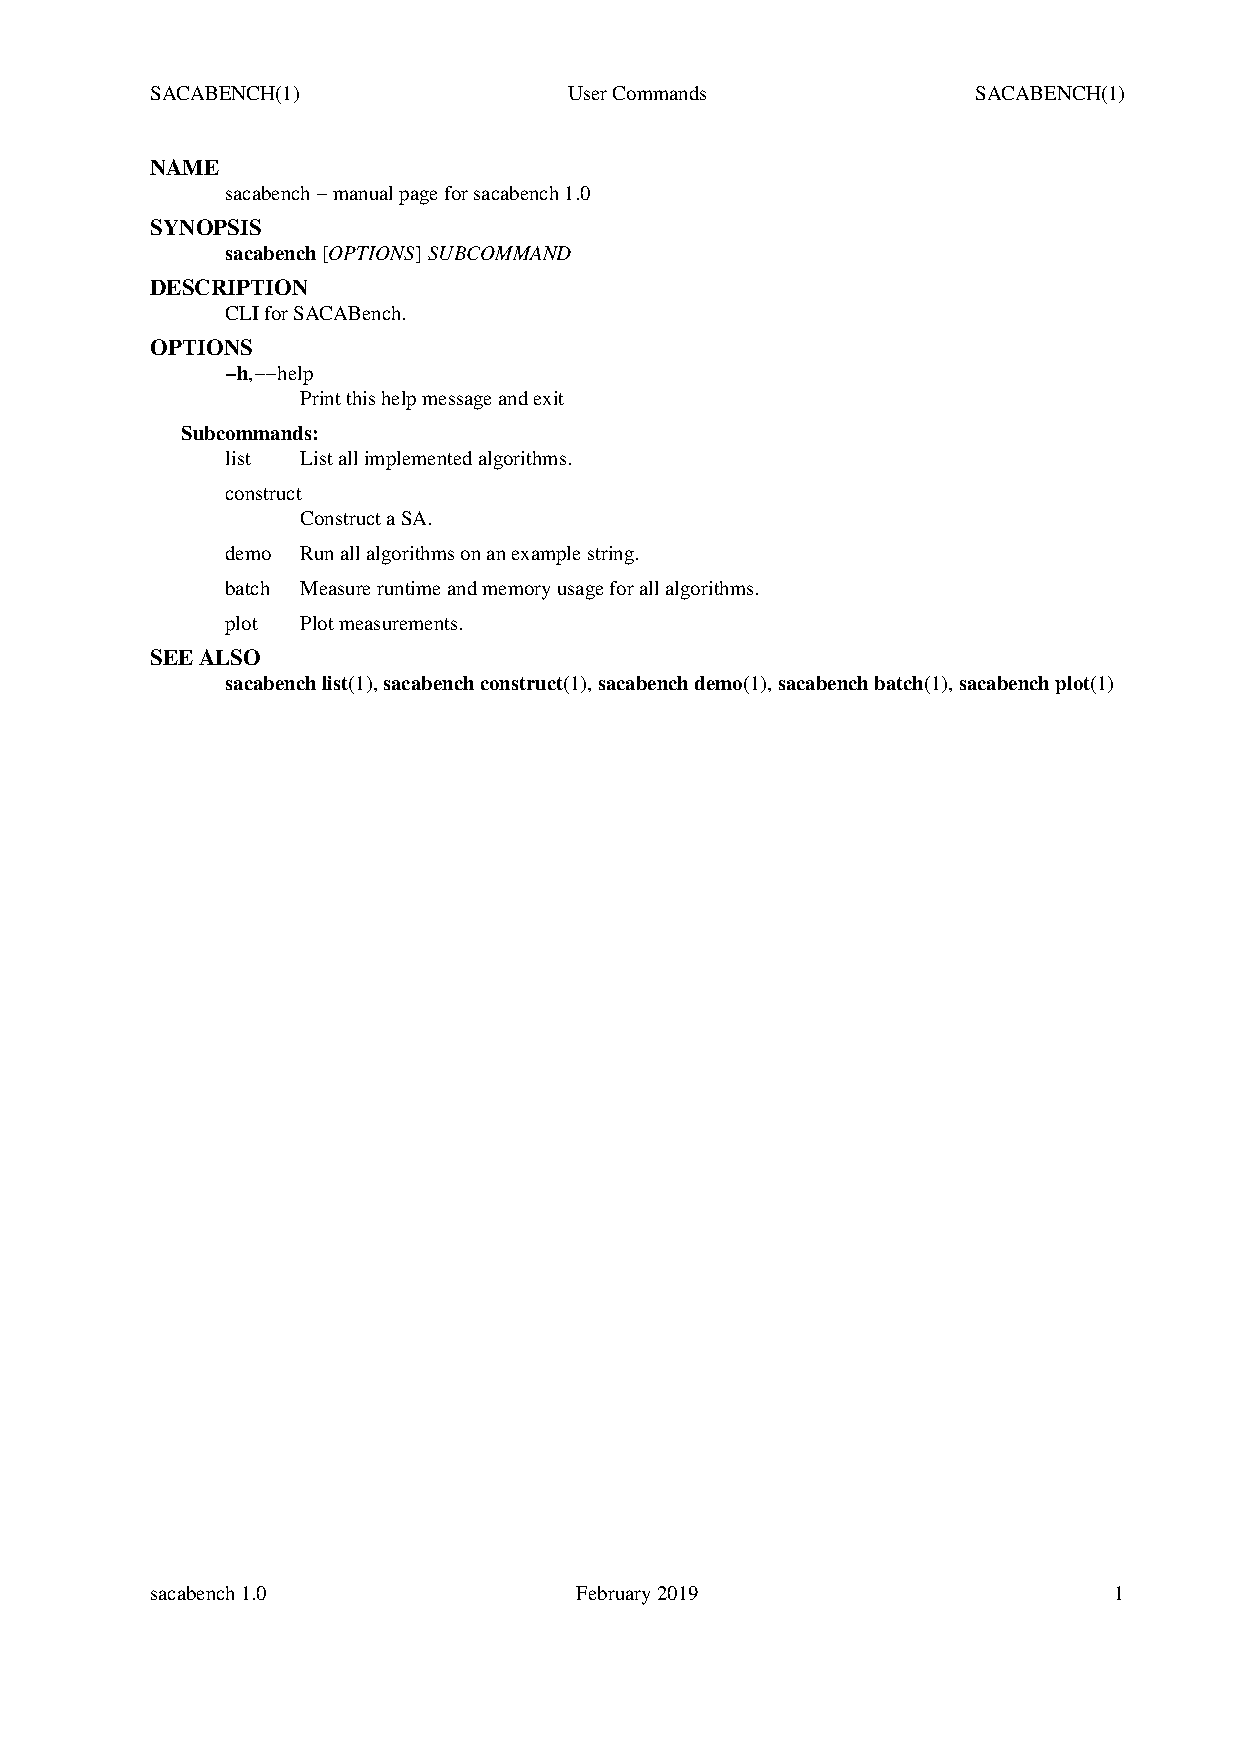
\includegraphics[clip, trim=10mm 20mm 10mm 10mm, page=1, frame, scale=0.70]{kapitel/3_framework/cli/manpages/sacabench.pdf}
\newpage

\section{sacabench list}
\label{manpage:sacabench-list}
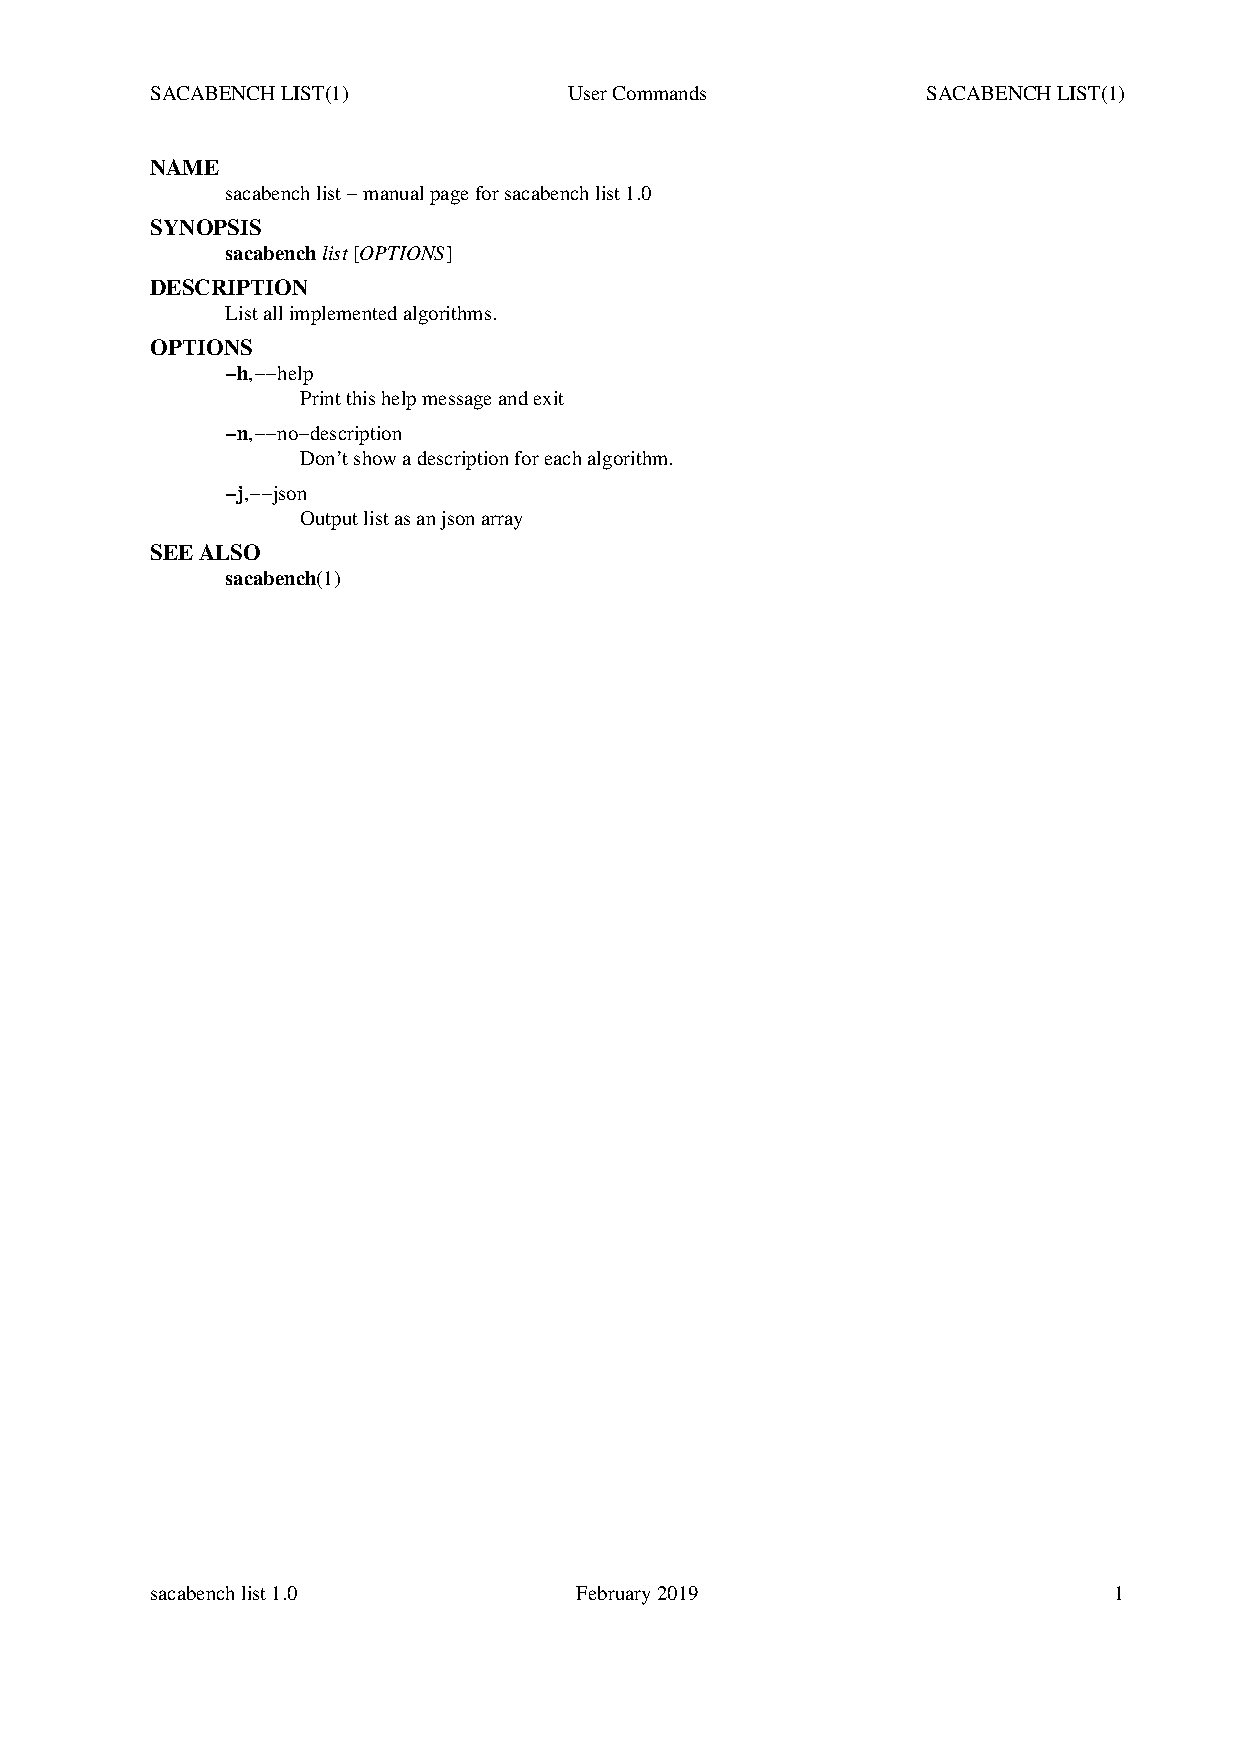
\includegraphics[clip, trim=10mm 20mm 10mm 10mm, page=1, frame, scale=0.70]{kapitel/3_framework/cli/manpages/sacabench-list.pdf}
\newpage

\section{sacabench demo}
\label{manpage:sacabench-demo}
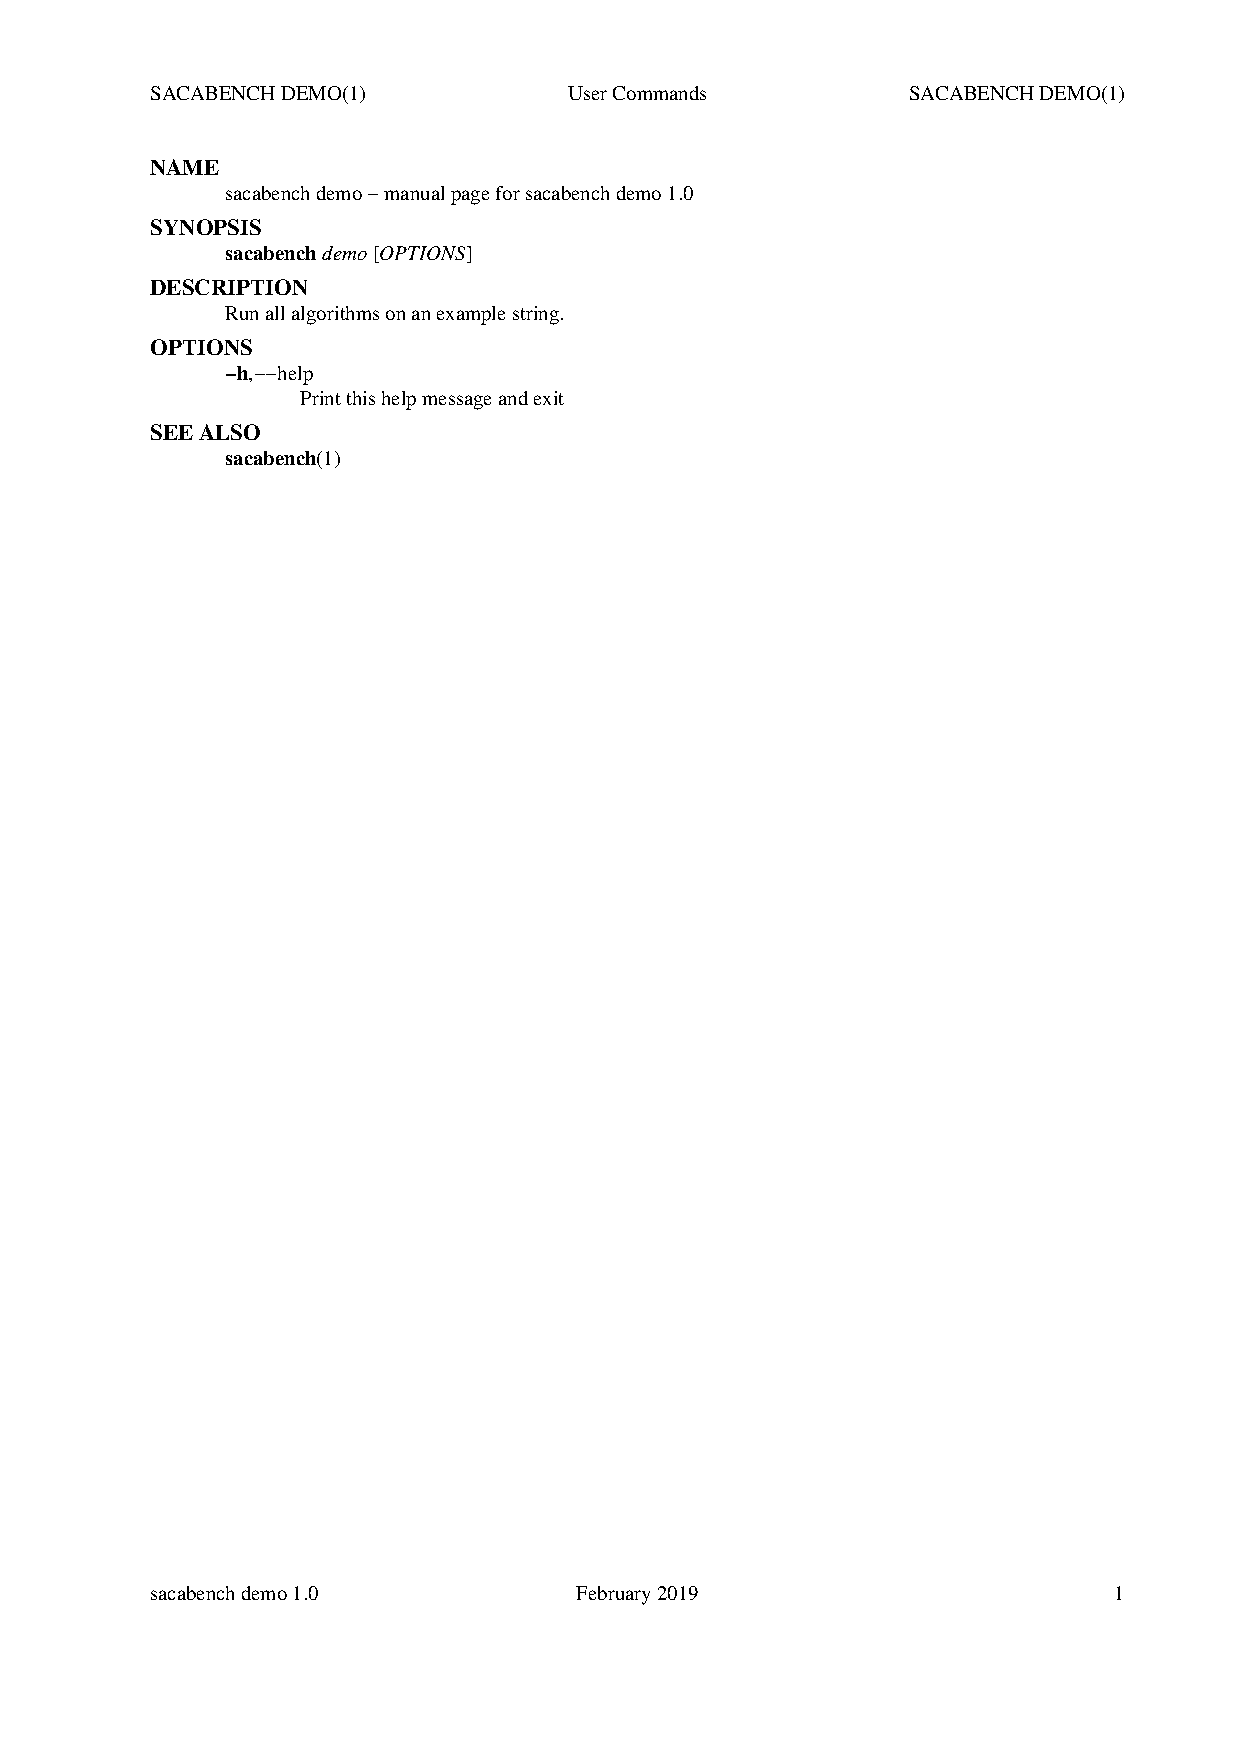
\includegraphics[clip, trim=10mm 20mm 10mm 10mm, page=1, frame, scale=0.70]{kapitel/3_framework/cli/manpages/sacabench-demo.pdf}
\newpage

\section{sacabench construct}
\label{manpage:sacabench-construct}
\includegraphics[clip, trim=10mm 20mm 10mm 10mm, page=1, frame, scale=0.70]{kapitel/3_framework/cli/manpages/sacabench-construct.pdf}
\newpage
\includegraphics[clip, trim=10mm 20mm 10mm 10mm, page=2, frame, scale=0.70]{kapitel/3_framework/cli/manpages/sacabench-construct.pdf}
\newpage

\section{sacabench batch}
\label{manpage:sacabench-batch}
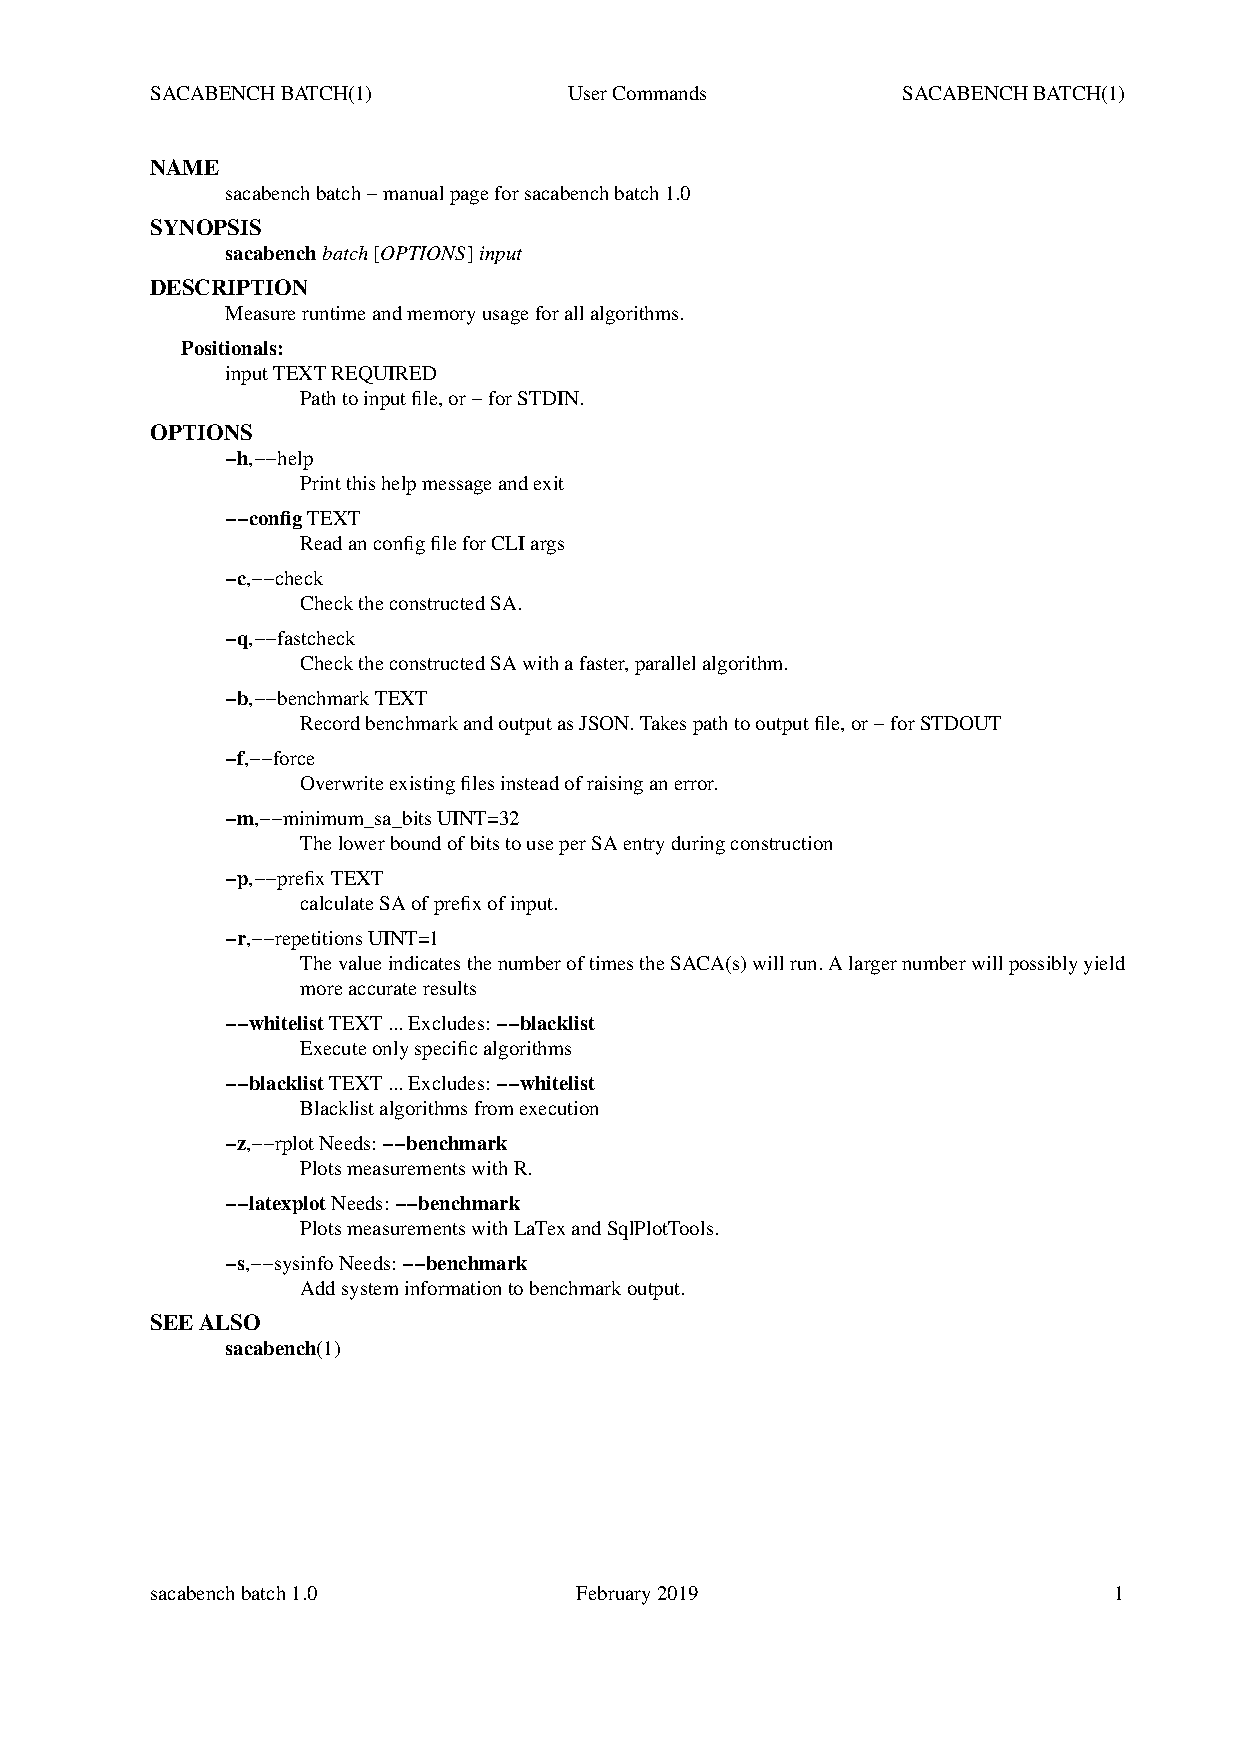
\includegraphics[clip, trim=10mm 20mm 10mm 10mm, page=1, frame, scale=0.70]{kapitel/3_framework/cli/manpages/sacabench-batch.pdf}
\newpage

\section{sacabench plot}
\label{manpage:sacabench-plot}
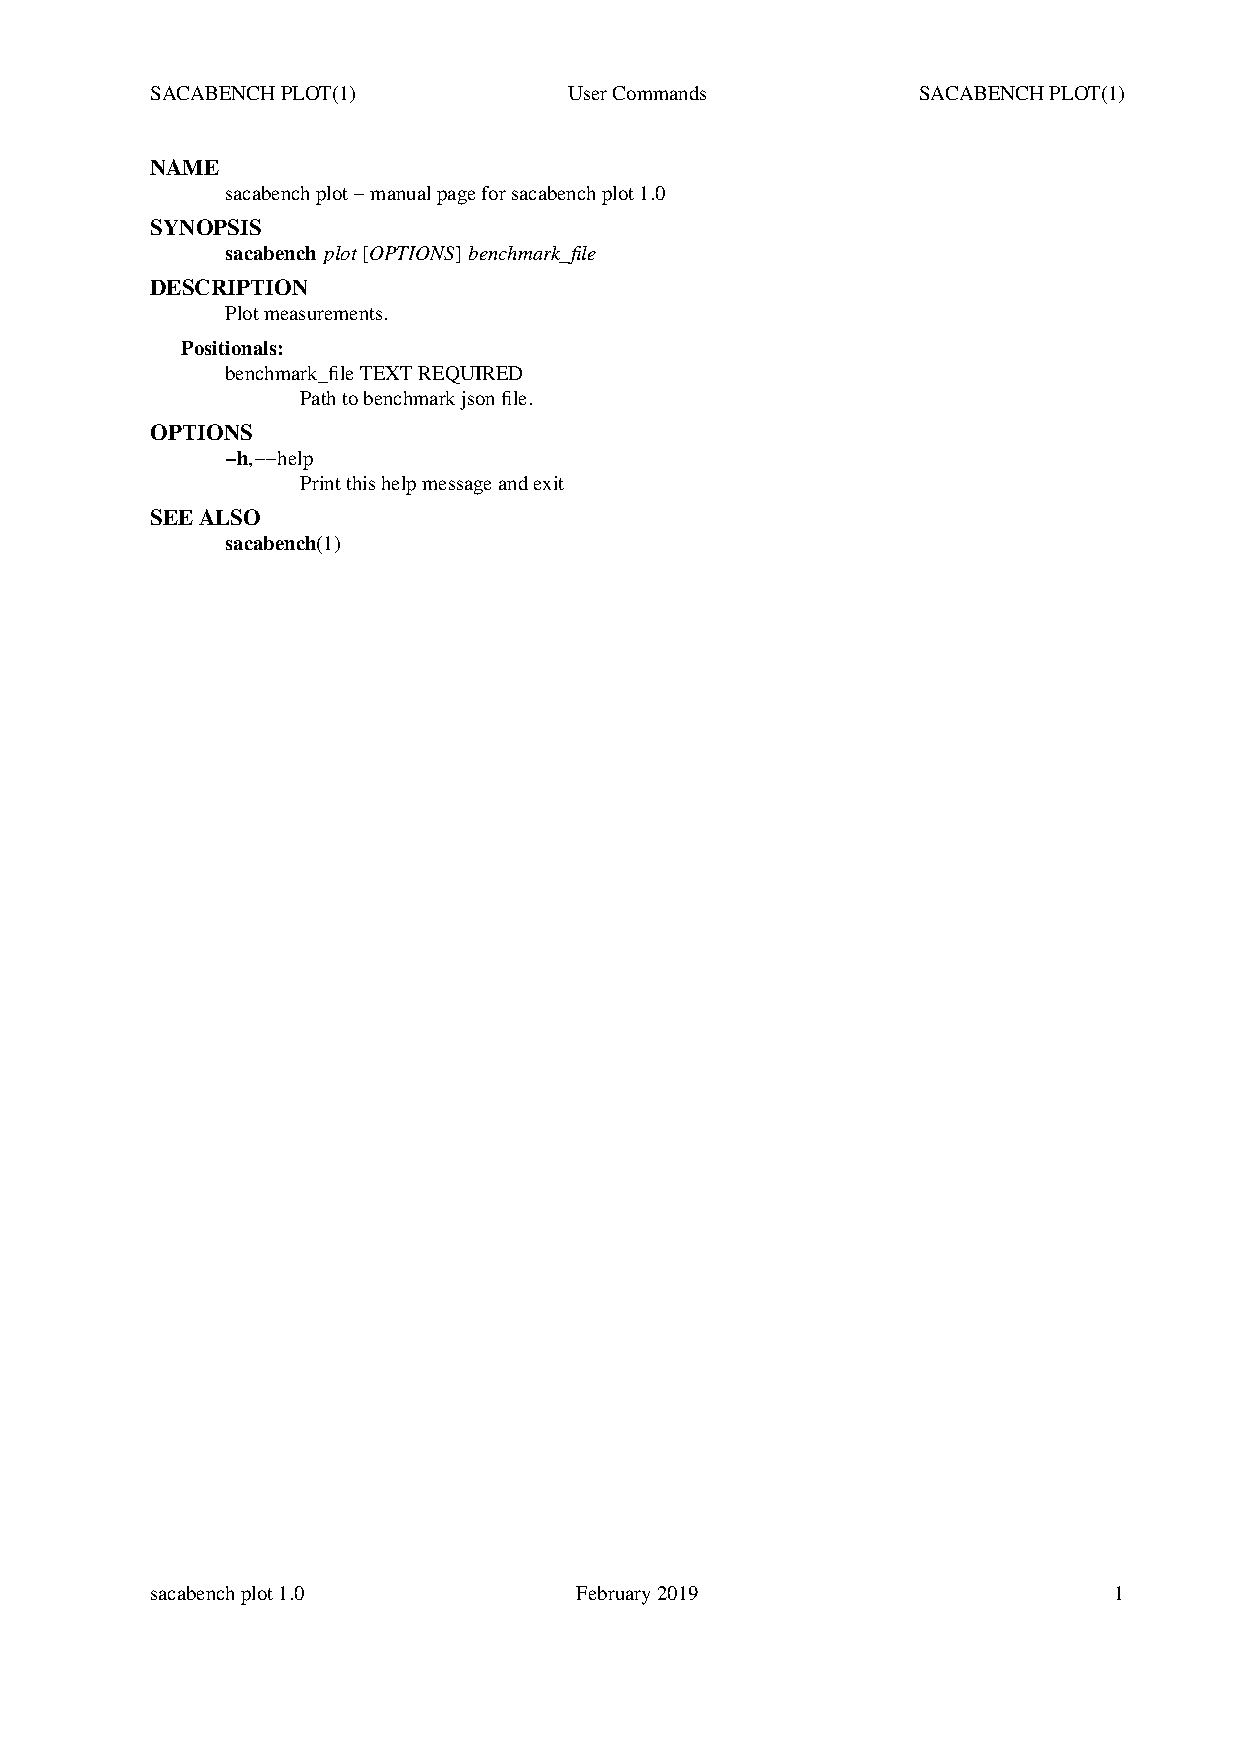
\includegraphics[clip, trim=10mm 20mm 10mm 10mm, page=1, frame, scale=0.70]{kapitel/3_framework/cli/manpages/sacabench-plot.pdf}


\bibliography{main}
\bibliographystyle{plainurl}

There are also some recursive algorithms, which mostly operate on a shared principle:
%
\paragraph{Recursive} Some algorithms such as DC3~\cite{saca:9} and SAIS~\cite{saca:6} require to sort a
partial set of suffixes as part of their task to sort the entire suffix array.
As they are able to do this by calling themselves with a different input, they are called \emph{recursive algorithms}.
DC3 sorts exactly $^2\!/\!_3$ of the suffixes by recursion, while SAIS sorts all the LMS suffixes by recursion,
if their ordering cannot be decided by looking at their first character.
After this step, the ordering of the other suffixes can be induced.

\begin{figure}[!t]
    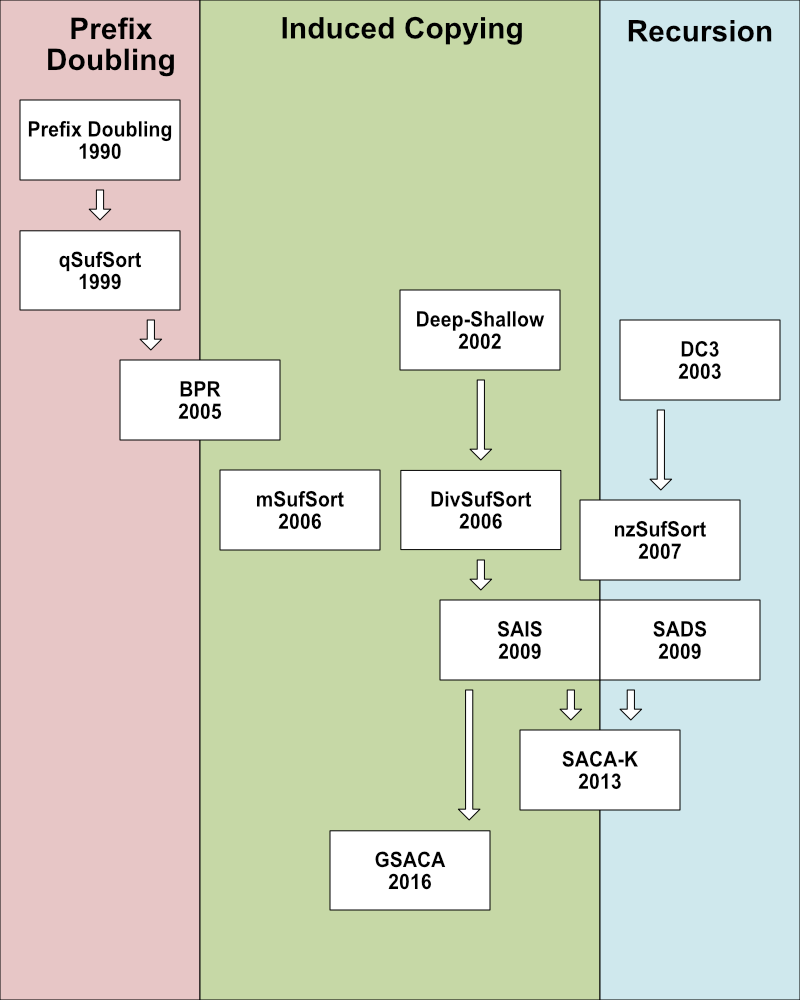
\includegraphics[width=\textwidth]{kapitel/5_saca_uebersicht/history/history3_eng.png}
    \caption{(partial) History of SACAs}
    \label{ea:fig:history}
\end{figure}

See Figure \ref{ea:fig:history} for a short summary of SACA history.
The different SACAs are divided into the three classes described above.
We now briefly explain the shown algorithms and their differences.

Prefix Doubling is a SACA which works purely by the above described method \emph{Doubling}.
In every iteration the \sa is refined and double the amount of characters are considered for sorting.
This directly influenced qSufSort, which improved its performance by using the \isa (inverse suffix arary) 
and subdividing suffixes into sorted and unsorted groups. 
BPR incorporated some ideas of inducing with prefix doubling and is therefore on the edge of those two paradigms.
Its inducing is based on the copy-technique by Seward~\cite{seward2000}.
This technique is also used by Deep-Shallow, which uses string-sorting instead of prefix doubling.
It influenced divsufsort, which sorts its RMS (rightmost S-Type) substrings before it completely sorts all RMS suffixes.
Given the correct order of the RMS suffixes, all remaining S-Type suffixes get induced in one and all L-Type suffixes in a second pass.
SAIS works by sorting all LMS (leftmost S-Type suffixes) in a recursion step before inducing the ordering of all suffixes in two passes similar to DivSufSort.
This is also done by SACA-K and GSACA, which are both similar to SAIS, but add some optimizations
(SACA-K for example doesn't use any extra space).
mSufSort is another inducing-SACA, but since it constructs the \isa instead of the \sa,
it's not derived from any other SACA.
The two other recursive SACAs are DC3 (which sorts $\frac{2}{3}$ of the suffixes in a recursion step)
and nzSufSort (which is similar to DC3 but improves on some aspects)\todo{nico? johannes? bitte ergänzen}.

\section{Optimization Strategies}

As with most programs, much of the performance of SACAs is dependent on efficiently implementing these algorithms.
We therefore used some practical optimizations to the descriptions of the algorithms to improve performance.
The following is an incomplete list of tricks one can use to do so.

\subsection{Different bit lengths for the suffix array}

We implemented our SACAs with an exchangable suffix array index type, that is a different bit length for the indices in the suffix array.
With our current implementation it is possible to use 32, 40, 48 and 64 bit for the suffix array elements.
Since our tool supports a different output encoding (32 or 64 bit), we can save memory during construction regardless of the desired output length.
Keep in mind that since the 40- and 48-bit types are not standardized, their performance is inferior to those of 32- and 64- bit types.

\subsection{Cache-efficiency}

The most crucial part of optimizing a SACA is cache-efficiency, that is aiming for time-local and space-local memory access.
Since the \sa is a pseudo-random mutation of numbers, it can't be written cache-efficiently.
However, when implementing SACAs, avoiding unnecessary cache misses can significantly improve performance.

\subsection{Wordpacking}

To maximize throughput, multiple characters of the input (8 bit each) can be processed as a whole by
interpreting them as integer numbers (64 bit, or even up to 512 bit by using vector operations).
Algorithms using wordpacking techniques are the Osipov algorithm~\cite{osipovGPU},
Doubling~\cite{saca:11}, Discarding~\cite{saca:11} and qSufSort~\cite{saca:1}.

\subsection{Utilization of a GPU}

Since modern GPUs feature higher degrees of parallelism compared to CPUs due to their architecture,
we include a prefix doubling SACA which uses CUDA and the CUB-Framework to run on the GPU~\cite{osipovGPU}.
We show that this algorithm outperformes the parallel DivSufSort implementation,
although the required and available memory on current GPUs still restricts the algorithm to far smaller input sizes than CPU SACAs are capable of.
Further research of GPU SACAs should be considered,
as we could hardly find any (working) reference algorithms to compare our implementation with, 
% Das hier sollte als Allgemeinwissen klar sein:
and development of GPUs shows higher performance improvements than CPU development in certain workloads.

\subsection{Sorting Algorithms}

Many SACAs use sorting algorithms at some point. For the benchmark a variety of sorting algorithms were implemented so that all SACAs can use them.
We include some versions of quicksort, bucketsort and radixsort.
This is especially interesting for naive parallelization, where one may just switch from a sequential sorting algorithm to a parallel one
and thereby improve performance.
Besides our own implemented sorting algorithms some external sorting algorithms are also included.
Most of those external sorting algorithms are made for parallel use.

\subsubsection{Binary vs. ternary comparison-based sort}

Multiple versions of quicksort are implemented:
Two of them are introsort~\cite{Musser97} and ternary quicksort~\cite{ternary_quicksort}.
It has been shown that the binary sorting procedure is faster,
if there are no equal elements in the set to be sorted~\cite{saca:4,ternary_quicksort};
otherwise, the ternary version is faster~\cite{ternary_quicksort}.
We therefore chose the best option for the required use-case.

\section{Evaluation}

Evaluation of both the sequential SACAs, including the reference algorithms, as well as of the parallel SACAs is done on LiDo3 \todo{Referenz}. The system's specifications are described in table \ref{system}.

\begin{table}
\caption{Messsystem}
\label{system}
\resizebox{\textwidth}{!}{
\begin{tabular}{ll}
\toprule
Operating System       & GNU/Linux \\
Kernel               & Linux \\
Kernel Release       & 3.10.0-862.14.4.el7.x86\_64 \\
Kernel Version       & \#1 SMP Wed Sep 26 15:12:11 UTC 2018 \\
\midrule
Architecture:        & x86\_64 \\
CPU op-mode(s):      & 32-bit, 64-bit \\
Byte Order:          & Little Endian \\
CPU(s):              & 20 \\
On-line CPU(s) list: & 0-19 \\
Thread(s) per core:  & 1 \\
Core(s) per socket:  & 10 \\
Socket(s):           & 2 \\
NUMA node(s):        & 2 \\
Vendor ID:           & GenuineIntel \\
CPU family:          & 6 \\
Model:               & 79 \\
Model name:          & Intel(R) Xeon(R) CPU E5-2640 v4 @ 2.40GHz \\
Stepping:            & 1 \\
CPU MHz:             & 2599.951 \\
CPU max MHz:         & 3400.0000 \\
CPU min MHz:         & 1200.0000 \\
BogoMIPS:            & 4789.01 \\
Virtualization:      & VT-x \\
L1d cache:           & 32K \\
L1i cache:           & 32K \\
L2 cache:            & 256K \\
L3 cache:            & 25600K \\
NUMA node0 CPU(s):   & 0-9 \\
NUMA node1 CPU(s):   & 10-19 \\
\midrule
Memory Size        & 64GiB \\
\bottomrule
\end{tabular}
}
\end{table}

\subsection{Evaluation (sequential)}

In the \crefrange{ea:runtime-all-0}{ea:runtime-all-2} we show the performance of the implementations of different SACAs on three texts.
The texts are \texttt{wiki.txt}, \texttt{dna.txt} and \texttt{commoncrawl.txt} from the \todo{was für ne quelle?} repository~\cite{xxx}.
\todo{Testsystem, Methodologie, ... (mb)}

\begin{figure}[!h]
    \textbf{Configuration} \hfill Input file: wiki.txt \hfill Prefix size: 1600\,MiB \\ Model name: Intel\textsuperscript{\textregistered} Xeon\textsuperscript{\textregistered} CPU E5-2640 v4 @ 2.40GHz
    \centering\small
    \begin{tikzpicture}[trim axis left]
        \begin{axis}[batchTimePlot,
            cycle list name={exotic},
            legend to name=runtime-all-ref-0,
            width=\textwidth,
            height=60mm,
            xtick style = {draw=none},
            xticklabel pos=upper,
            title={},
            bar width=12pt,
            ylabel={\sa construction time [min]},
            legend style={
                /tikz/every even column/.append style={column sep=0.5cm,black},
                /tikz/every even column/.append style={black},
            },
            legend columns=2,
            symbolic x coords={ wiki.txt },
            every node near coord/.append style={color=black, rotate=90, anchor=west},
            ]

            %% MULTIPLOT(algo) SELECT algo, REPLACE(input, "_", "\_") AS x, time/1000/60 AS y
            %% FROM ( 
            %% SELECT algo, input, MEDIAN(memFinal) AS memFinal, MEDIAN(memOff) AS memOff, AVG(memPeak) AS memPeak, prefix, rep_id, MEDIAN(time) AS time FROM results_sequential GROUP BY algo, input, prefix, rep_id
            %% ) WHERE input="wiki.txt" AND prefix=1677721600
            %% AND (algo LIKE "%_ref%" AND NOT algo LIKE "%par")
            %% AND rep_id=1 GROUP BY MULTIPLOT,x ORDER BY y
            \addplot coordinates { (wiki.txt,3.45026) };
            \addlegendentry{algo=DivSufSort\_ref};
            \addplot coordinates { (wiki.txt,5.80588) };
            \addlegendentry{algo=SAIS-LITE\_ref};
            \addplot coordinates { (wiki.txt,6.33265) };
            \addlegendentry{algo=BPR\_ref};
            \addplot coordinates { (wiki.txt,10.5834) };
            \addlegendentry{algo=SACA-K\_ref};
            \addplot coordinates { (wiki.txt,13.9982) };
            \addlegendentry{algo=qsufsort\_ref};
            \addplot coordinates { (wiki.txt,15.3998) };
            \addlegendentry{algo=SAIS\_ref};
            \addplot coordinates { (wiki.txt,18.5135) };
            \addlegendentry{algo=GSACA\_ref};
            \addplot coordinates { (wiki.txt,19.0941) };
            \addlegendentry{algo=SADS\_ref};
            \addplot coordinates { (wiki.txt,62.1154) };
            \addlegendentry{algo=DC3\_ref};
        \end{axis}
    \end{tikzpicture}
    \begin{tikzpicture}[trim axis left]
        \begin{axis}[batchTimePlot,
            cycle list name={exotic},
            width=\textwidth,
            height=60mm,
            xtick style = {draw=none},
            y dir=reverse,
            title={},
            bar width=12pt,
            ylabel={Extra Memory [GiB]},
            legend style={
                /tikz/every even column/.append style={column sep=0.5cm,black},
                /tikz/every even column/.append style={black},
            },
            legend columns=2,
            symbolic x coords={ wiki.txt },
            every node near coord/.append style={color=black, rotate=90, anchor=east, /pgf/number format/fixed},
            ]

            %% MULTIPLOT(algo) SELECT algo, REPLACE(input, "_", "\_") AS x, memPeak/1024/1024/1024 AS y
            %% FROM ( 
            %% SELECT algo, input, MEDIAN(memFinal) AS memFinal, MEDIAN(memOff) AS memOff, AVG(memPeak) AS memPeak, prefix, rep_id, MEDIAN(time) AS time FROM results_sequential GROUP BY algo, input, prefix, rep_id
            %% ) WHERE input="wiki.txt" AND prefix=1677721600
            %% AND (algo LIKE "%_ref%" AND NOT algo LIKE "%par")
            %% AND rep_id=1 GROUP BY MULTIPLOT,x ORDER BY time
            \addplot coordinates { (wiki.txt,0.000252061) };
            \addlegendentry{algo=DivSufSort\_ref};
            \addplot coordinates { (wiki.txt,6.25) };
            \addlegendentry{algo=SAIS-LITE\_ref};
            \addplot coordinates { (wiki.txt,26.6305) };
            \addlegendentry{algo=BPR\_ref};
            \addplot coordinates { (wiki.txt,7.82311e-07) };
            \addlegendentry{algo=SACA-K\_ref};
            \addplot coordinates { (wiki.txt,25) };
            \addlegendentry{algo=qsufsort\_ref};
            \addplot coordinates { (wiki.txt,0.499429) };
            \addlegendentry{algo=SAIS\_ref};
            \addplot coordinates { (wiki.txt,18.75) };
            \addlegendentry{algo=GSACA\_ref};
            \addplot coordinates { (wiki.txt,0.661858) };
            \addlegendentry{algo=SADS\_ref};
            \addplot coordinates { (wiki.txt,36.7684) };
            \addlegendentry{algo=DC3\_ref};

            \legend{}
        \end{axis}
    \end{tikzpicture}
    \medskip
    \ref{runtime-all-ref-0}
    \caption{Comparison of the in \sacabench included reference implementations of SACAs, including time and memory consumption: wiki.txt}
    \ref{ea:runtime-all-ref-0}
\end{figure}

\begin{figure}[!h]
    \textbf{Configuration} \hfill Input file: dna.txt \hfill Prefix size: 1600\,MiB \\ Model name: Intel\textsuperscript{\textregistered} Xeon\textsuperscript{\textregistered} CPU E5-2640 v4 @ 2.40GHz
    \centering\small
    \begin{tikzpicture}[trim axis left]
        \begin{axis}[batchTimePlot,
            cycle list name={exotic},
            legend to name=runtime-all-ref-1,
            width=\textwidth,
            height=60mm,
            xtick style = {draw=none},
            xticklabel pos=upper,
            title={},
            bar width=12pt,
            ylabel={\sa construction time [min]},
            legend style={
                /tikz/every even column/.append style={column sep=0.5cm,black},
                /tikz/every even column/.append style={black},
            },
            legend columns=2,
            symbolic x coords={ dna.txt },
            every node near coord/.append style={color=black, rotate=90, anchor=west},
            ]

            %% MULTIPLOT(algo) SELECT algo, REPLACE(input, "_", "\_") AS x, time/1000/60 AS y
            %% FROM ( 
            %% SELECT algo, input, MEDIAN(memFinal) AS memFinal, MEDIAN(memOff) AS memOff, AVG(memPeak) AS memPeak, prefix, rep_id, MEDIAN(time) AS time FROM results_sequential GROUP BY algo, input, prefix, rep_id
            %% ) WHERE input="dna.txt" AND prefix=1677721600
            %% AND (algo LIKE "%_ref%" AND NOT algo LIKE "%par")
            %% AND rep_id=1 GROUP BY MULTIPLOT,x ORDER BY y
            \addplot coordinates { (dna.txt,4.25621) };
            \addlegendentry{algo=DivSufSort\_ref};
            \addplot coordinates { (dna.txt,4.93084) };
            \addlegendentry{algo=Deep-Shallow\_ref};
            \addplot coordinates { (dna.txt,6.05679) };
            \addlegendentry{algo=SAIS-LITE\_ref};
            \addplot coordinates { (dna.txt,7.45044) };
            \addlegendentry{algo=BPR\_ref};
            \addplot coordinates { (dna.txt,10.0834) };
            \addlegendentry{algo=SACA-K\_ref};
            \addplot coordinates { (dna.txt,11.7436) };
            \addlegendentry{algo=qsufsort\_ref};
            \addplot coordinates { (dna.txt,13.6695) };
            \addlegendentry{algo=GSACA\_ref};
            \addplot coordinates { (dna.txt,14.4639) };
            \addlegendentry{algo=SAIS\_ref};
            \addplot coordinates { (dna.txt,19.4301) };
            \addlegendentry{algo=SADS\_ref};
            \addplot coordinates { (dna.txt,41.2953) };
            \addlegendentry{algo=DC3\_ref};
        \end{axis}
    \end{tikzpicture}
    \begin{tikzpicture}[trim axis left]
        \begin{axis}[batchTimePlot,
            cycle list name={exotic},
            width=\textwidth,
            height=60mm,
            xtick style = {draw=none},
            y dir=reverse,
            title={},
            bar width=12pt,
            ylabel={Extra Memory [GiB]},
            legend style={
                /tikz/every even column/.append style={column sep=0.5cm,black},
                /tikz/every even column/.append style={black},
            },
            legend columns=2,
            symbolic x coords={ dna.txt },
            every node near coord/.append style={color=black, rotate=90, anchor=east, /pgf/number format/fixed},
            ]

            %% MULTIPLOT(algo) SELECT algo, REPLACE(input, "_", "\_") AS x, memPeak/1024/1024/1024 AS y
            %% FROM ( 
            %% SELECT algo, input, MEDIAN(memFinal) AS memFinal, MEDIAN(memOff) AS memOff, AVG(memPeak) AS memPeak, prefix, rep_id, MEDIAN(time) AS time FROM results_sequential GROUP BY algo, input, prefix, rep_id
            %% ) WHERE input="dna.txt" AND prefix=1677721600
            %% AND (algo LIKE "%_ref%" AND NOT algo LIKE "%par")
            %% AND rep_id=1 GROUP BY MULTIPLOT,x ORDER BY time
            \addplot coordinates { (dna.txt,0.000252061) };
            \addlegendentry{algo=DivSufSort\_ref};
            \addplot coordinates { (dna.txt,0.01875) };
            \addlegendentry{algo=Deep-Shallow\_ref};
            \addplot coordinates { (dna.txt,6.25) };
            \addlegendentry{algo=SAIS-LITE\_ref};
            \addplot coordinates { (dna.txt,26.5626) };
            \addlegendentry{algo=BPR\_ref};
            \addplot coordinates { (dna.txt,1.86265e-08) };
            \addlegendentry{algo=SACA-K\_ref};
            \addplot coordinates { (dna.txt,25) };
            \addlegendentry{algo=qsufsort\_ref};
            \addplot coordinates { (dna.txt,18.75) };
            \addlegendentry{algo=GSACA\_ref};
            \addplot coordinates { (dna.txt,0.481298) };
            \addlegendentry{algo=SAIS\_ref};
            \addplot coordinates { (dna.txt,0.658049) };
            \addlegendentry{algo=SADS\_ref};
            \addplot coordinates { (dna.txt,35.0308) };
            \addlegendentry{algo=DC3\_ref};

            \legend{}
        \end{axis}
    \end{tikzpicture}
    \medskip
    \ref{runtime-all-ref-1}
    \caption{Comparison of the in \sacabench included reference implementations of SACAs, including time and memory consumption: dna.txt}
    \ref{ea:runtime-all-ref-1}
\end{figure}

\begin{figure}[!h]
    \textbf{Configuration} \hfill Input file: commoncrawl.txt \hfill Prefix size: 1600\,MiB \\ Model name: Intel\textsuperscript{\textregistered} Xeon\textsuperscript{\textregistered} CPU E5-2640 v4 @ 2.40GHz
    \centering\small
    \begin{tikzpicture}[trim axis left]
        \begin{axis}[batchTimePlot,
            cycle list name={exotic},
            legend to name=runtime-all-ref-2,
            width=\textwidth,
            height=60mm,
            xtick style = {draw=none},
            xticklabel pos=upper,
            title={},
            bar width=12pt,
            ylabel={\sa construction time [min]},
            legend style={
                /tikz/every even column/.append style={column sep=0.5cm,black},
                /tikz/every even column/.append style={black},
            },
            legend columns=2,
            symbolic x coords={ commoncrawl.txt },
            every node near coord/.append style={color=black, rotate=90, anchor=west},
            ]

            %% MULTIPLOT(algo) SELECT algo, REPLACE(input, "_", "\_") AS x, time/1000/60 AS y
            %% FROM ( 
            %% SELECT algo, input, MEDIAN(memFinal) AS memFinal, MEDIAN(memOff) AS memOff, AVG(memPeak) AS memPeak, prefix, rep_id, MEDIAN(time) AS time FROM results_sequential GROUP BY algo, input, prefix, rep_id
            %% ) WHERE input="commoncrawl.txt" AND prefix=1677721600
            %% AND (algo LIKE "%_ref%" AND NOT algo LIKE "%par")
            %% AND rep_id=1 GROUP BY MULTIPLOT,x ORDER BY y
            \addplot coordinates { (commoncrawl.txt,3.19154) };
            \addlegendentry{algo=DivSufSort\_ref};
            \addplot coordinates { (commoncrawl.txt,4.91103) };
            \addlegendentry{algo=SAIS-LITE\_ref};
            \addplot coordinates { (commoncrawl.txt,5.03779) };
            \addlegendentry{algo=BPR\_ref};
            \addplot coordinates { (commoncrawl.txt,9.45164) };
            \addlegendentry{algo=SACA-K\_ref};
            \addplot coordinates { (commoncrawl.txt,13.0888) };
            \addlegendentry{algo=SAIS\_ref};
            \addplot coordinates { (commoncrawl.txt,15.3615) };
            \addlegendentry{algo=GSACA\_ref};
            \addplot coordinates { (commoncrawl.txt,15.4028) };
            \addlegendentry{algo=qsufsort\_ref};
            \addplot coordinates { (commoncrawl.txt,16.5888) };
            \addlegendentry{algo=SADS\_ref};
            \addplot coordinates { (commoncrawl.txt,60.4603) };
            \addlegendentry{algo=DC3\_ref};
        \end{axis}
    \end{tikzpicture}
    \begin{tikzpicture}[trim axis left]
        \begin{axis}[batchTimePlot,
            cycle list name={exotic},
            width=\textwidth,
            height=60mm,
            xtick style = {draw=none},
            y dir=reverse,
            title={},
            bar width=12pt,
            ylabel={Extra Memory [GiB]},
            legend style={
                /tikz/every even column/.append style={column sep=0.5cm,black},
                /tikz/every even column/.append style={black},
            },
            legend columns=2,
            symbolic x coords={ commoncrawl.txt },
            every node near coord/.append style={color=black, rotate=90, anchor=east, /pgf/number format/fixed},
            ]

            %% MULTIPLOT(algo) SELECT algo, REPLACE(input, "_", "\_") AS x, memPeak/1024/1024/1024 AS y
            %% FROM ( 
            %% SELECT algo, input, MEDIAN(memFinal) AS memFinal, MEDIAN(memOff) AS memOff, AVG(memPeak) AS memPeak, prefix, rep_id, MEDIAN(time) AS time FROM results_sequential GROUP BY algo, input, prefix, rep_id
            %% ) WHERE input="commoncrawl.txt" AND prefix=1677721600
            %% AND (algo LIKE "%_ref%" AND NOT algo LIKE "%par")
            %% AND rep_id=1 GROUP BY MULTIPLOT,x ORDER BY time
            \addplot coordinates { (commoncrawl.txt,0.000252061) };
            \addlegendentry{algo=DivSufSort\_ref};
            \addplot coordinates { (commoncrawl.txt,6.25) };
            \addlegendentry{algo=SAIS-LITE\_ref};
            \addplot coordinates { (commoncrawl.txt,26.6681) };
            \addlegendentry{algo=BPR\_ref};
            \addplot coordinates { (commoncrawl.txt,9.05246e-07) };
            \addlegendentry{algo=SACA-K\_ref};
            \addplot coordinates { (commoncrawl.txt,0.498627) };
            \addlegendentry{algo=SAIS\_ref};
            \addplot coordinates { (commoncrawl.txt,18.75) };
            \addlegendentry{algo=GSACA\_ref};
            \addplot coordinates { (commoncrawl.txt,25) };
            \addlegendentry{algo=qsufsort\_ref};
            \addplot coordinates { (commoncrawl.txt,0.634287) };
            \addlegendentry{algo=SADS\_ref};
            \addplot coordinates { (commoncrawl.txt,37.3555) };
            \addlegendentry{algo=DC3\_ref};

            \legend{}
        \end{axis}
    \end{tikzpicture}
    \medskip
    \ref{runtime-all-ref-2}
    \caption{Comparison of the in \sacabench included reference implementations of SACAs, including time and memory consumption: commoncrawl.txt}
    \ref{ea:runtime-all-ref-2}
\end{figure}
\FloatBarrier

The clear winners in all three cases is divsufsort, followed by BPR and SAIS-Lite
\footnote{divsufsort and SAIS-Lite both are optimized implementations by Yuta Mori~\cite{saca:5}.}.
In terms of memory consumption, divsufsort and SACA-K are the two best algorithms since they use no extra space,
follwed by Deep-Shallow\_ref, which uses very little extra space.
The worst algorithm in both runtime performance as well as memory consumption is in all three cases the reference implementation of DC3,
which is followed by SADS (a variant of SAIS~\cite{saca:6}) in terms of performance and BPR in terms of memory consumption.

\todo{beschreibung der algorithmen im mittelfeld (mb)}
\todo{@johannes wieso ist dc3 so scheiße? (mb)}
\todo{@flo wieso hat bpr soviel speicher? (mb)}
\todo{wieso taucht deep shallow nur auf dna auf? (mb)}
\todo{vermisst jemand seine ref komplett? (mb)}

\subsection{Evaluation (parallel)}

In this section we will compare the performance of the runtime and memory performance of the included parallel SACAs.
These are variants of the sequential algorithms, that were mostly naively parallelized, with the exception of parallel SAIS
\footnote{This algorithm uses read/write buffers and a parallel pipeline based on work of Lao et al~\cite{psais}.}.

\begin{figure}[!h]
    \centering
    \begin{tikzpicture}[trim axis left]
        \begin{axis}[
                name=axis1,
                cycle list name={exoticlines},
                width=\textwidth,
                height=60mm,
                title={wiki.txt},
                xlabel={num threads, input size [200\,MB]},
                ylabel={SA construction time [min]},
                legend columns=2,
                legend to name=legend-par-all-0,
                legend style={
                    /tikz/every even column/.append style={column sep=0.5cm,black},
                    /tikz/every even column/.append style={black},
                },
            ]

            %% MULTIPLOT(algo) SELECT thread_count AS x, time/1000/60 AS y, MULTIPLOT
            %% FROM (
            %% SELECT algo, input, MEDIAN(memFinal) AS memFinal, MEDIAN(memOff) AS memOff, AVG(memPeak) AS memPeak, prefix, rep, thread_count, MEDIAN(time) AS time, sacheck FROM stats_parallel GROUP BY algo, input, prefix, rep, thread_count
            %% ) WHERE input="wiki.txt" AND sacheck="ok"
            %% AND (algo="BPR_par" OR algo="DC3-Parallel-V2" OR algo="NaivParallel" OR algo="Deep-Shallow_par" OR algo="Discarding2Parallel" OR algo="Discarding4Parallel" OR algo="PARALLEL_SAIS")
            %% GROUP BY MULTIPLOT,x ORDER BY MULTIPLOT,x
            \addplot coordinates { (1,0.543257) (2,1.04248) (4,2.69455) (8,5.00914) (12,8.55647) (16,12.5204) };
            \addlegendentry{algo=BPR\_par};
            \addplot coordinates { (1,3.09365) (2,4.11916) (4,5.55123) (8,7.75629) };
            \addlegendentry{algo=DC3-Parallel-V2};
            \addplot coordinates { (1,1.41234) (2,1.79674) (4,2.28839) (8,3.29598) (12,4.53346) (16,5.42954) (20,6.48599) };
            \addlegendentry{algo=Deep-Shallow\_par};
            \addplot coordinates { (1,3.20359) (2,3.69207) (4,4.44643) (8,5.90081) };
            \addlegendentry{algo=Discarding2Parallel};
            \addplot coordinates { (1,2.32532) (2,2.82934) (4,3.37798) (8,4.41391) };
            \addlegendentry{algo=Discarding4Parallel};
            \addplot coordinates { (1,2.71662) (2,3.54087) (4,4.03271) (8,4.7199) (12,5.55871) (16,5.86449) };
            \addlegendentry{algo=NaivParallel};
            \addplot coordinates { (1,1.07199) (2,2.15225) (4,4.661) (8,10.5053) };
            \addlegendentry{algo=PARALLEL\_SAIS};
        \end{axis}
    \end{tikzpicture}
    \par\bigskip
    \begin{tikzpicture}[trim axis left]
        \begin{axis}[
                cycle list name={exoticlines},
                at={(axis1.outer north east)},
                anchor=outer north west,
                name=axis2,
                width=\textwidth,
                height=60mm,
                title={wiki.txt},
                xlabel={num threads, input size [200\,MB]},
                ylabel={Extra Memory [GiB]},
            ]

            %% MULTIPLOT(algo) SELECT thread_count AS x, memPeak/1024/1024/1024 AS y, MULTIPLOT
            %% FROM (
            %% SELECT algo, input, MEDIAN(memFinal) AS memFinal, MEDIAN(memOff) AS memOff, AVG(memPeak) AS memPeak, prefix, rep, thread_count, MEDIAN(time) AS time, sacheck FROM stats_parallel GROUP BY algo, input, prefix, rep, thread_count
            %% ) WHERE input="wiki.txt" AND sacheck="ok"
            %% AND (algo="BPR_par" OR algo="DC3-Parallel-V2" OR algo="NaivParallel" OR algo="Deep-Shallow_par" OR algo="Discarding2Parallel" OR algo="Discarding4Parallel" OR algo="PARALLEL_SAIS")
            %% GROUP BY MULTIPLOT,x ORDER BY MULTIPLOT,x
            \addplot coordinates { (1,0.951951) (2,1.7332) (4,3.4355) (8,6.83651) (12,19.647) (16,26.173) };
            \addlegendentry{algo=BPR\_par};
            \addplot coordinates { (1,3.10468) (2,8.33334) (4,16.6667) (8,31.9445) };
            \addlegendentry{algo=DC3-Parallel-V2};
            \addplot coordinates { (1,0.00319003) (2,0.00532148) (4,0.00959451) (8,0.0183557) (12,0.0497788) (16,0.0630637) (20,0.0779177) };
            \addlegendentry{algo=Deep-Shallow\_par};
            \addplot coordinates { (1,2.34575) (2,4.69158) (4,9.38307) (8,18.766) };
            \addlegendentry{algo=Discarding2Parallel};
            \addplot coordinates { (1,3.90825) (2,7.81659) (4,15.6331) (8,31.2661) };
            \addlegendentry{algo=Discarding4Parallel};
            \addplot coordinates { (1,0.0) (2,1.5625) (4,3.12501) (8,6.25002) (12,18.75) (16,25) };
            \addlegendentry{algo=NaivParallel};
            \addplot coordinates { (1,0.416671) (2,0.524891) (4,0.731684) (8,1.10245) };
            \addlegendentry{algo=PARALLEL\_SAIS};

            \legend{}
        \end{axis}
    \end{tikzpicture}

    \medskip
    \ref{legend-par-all-0}
    \caption{Vergleich der parallelen Implementierungen mit Laufzeit und Speicherbedarf auf wiki.txt}
    \label{fig-par-all-0}
\end{figure}

\begin{figure}[!h]
    \centering
    \begin{tikzpicture}[trim axis left]
        \begin{axis}[
                name=axis1,
                cycle list name={exoticlines},
                width=\textwidth,
                height=60mm,
                title={dna.txt},
                xlabel={num threads, input size [200\,MB]},
                ylabel={SA construction time [min]},
                legend columns=2,
                legend to name=legend-par-all-1,
                legend style={
                    /tikz/every even column/.append style={column sep=0.5cm,black},
                    /tikz/every even column/.append style={black},
                },
            ]

            %% MULTIPLOT(algo) SELECT thread_count AS x, time/1000/60 AS y, MULTIPLOT
            %% FROM (
            %% SELECT algo, input, MEDIAN(memFinal) AS memFinal, MEDIAN(memOff) AS memOff, AVG(memPeak) AS memPeak, prefix, rep, thread_count, MEDIAN(time) AS time, sacheck FROM stats_parallel GROUP BY algo, input, prefix, rep, thread_count
            %% ) WHERE input="dna.txt" AND sacheck="ok"
            %% AND (algo="BPR_par" OR algo="DC3-Parallel-V2" OR algo="NaivParallel" OR algo="Deep-Shallow_par" OR algo="Discarding2Parallel" OR algo="Discarding4Parallel" OR algo="PARALLEL_SAIS")
            %% GROUP BY MULTIPLOT,x ORDER BY MULTIPLOT,x
            \addplot coordinates { (1,0.569637) (2,1.09372) (4,2.16083) (8,4.4065) (12,8.71249) (16,11.9082) };
            \addlegendentry{algo=BPR\_par};
            \addplot coordinates { (1,3.02187) (2,3.97795) (4,5.28252) (8,7.08082) };
            \addlegendentry{algo=DC3-Parallel-V2};
            \addplot coordinates { (1,1.84653) (2,2.47075) (4,3.2711) (8,4.23853) (12,5.92934) (16,9.05611) (20,10.8896) };
            \addlegendentry{algo=Deep-Shallow\_par};
            \addplot coordinates { (1,3.2561) (2,3.83204) (4,4.51572) (8,5.42115) };
            \addlegendentry{algo=Discarding2Parallel};
            \addplot coordinates { (1,2.50936) (2,3.04948) (4,3.62786) (8,4.52356) };
            \addlegendentry{algo=Discarding4Parallel};
            \addplot coordinates { (1,3.06848) (2,4.3148) (4,4.73058) (8,5.05918) (12,5.68415) (16,5.68597) };
            \addlegendentry{algo=NaivParallel};
            \addplot coordinates { (1,1.11013) (2,2.02917) (4,4.40177) (8,9.565) };
            \addlegendentry{algo=PARALLEL\_SAIS};

        \end{axis}
    \end{tikzpicture}
    \par\bigskip
    \begin{tikzpicture}[trim axis left]
        \begin{axis}[
                cycle list name={exoticlines},
                at={(axis1.outer north east)},
                anchor=outer north west,
                name=axis2,
                width=\textwidth,
                height=60mm,
                title={dna.txt},
                xlabel={num threads, input size [200\,MB]},
                ylabel={Extra Memory [GiB]},
            ]

            %% MULTIPLOT(algo) SELECT thread_count AS x, memPeak/1024/1024/1024 AS y, MULTIPLOT
            %% FROM (
            %% SELECT algo, input, MEDIAN(memFinal) AS memFinal, MEDIAN(memOff) AS memOff, AVG(memPeak) AS memPeak, prefix, rep, thread_count, MEDIAN(time) AS time, sacheck FROM stats_parallel GROUP BY algo, input, prefix, rep, thread_count
            %% ) WHERE input="dna.txt" AND sacheck="ok"
            %% AND (algo="BPR_par" OR algo="DC3-Parallel-V2" OR algo="NaivParallel" OR algo="Deep-Shallow_par" OR algo="Discarding2Parallel" OR algo="Discarding4Parallel" OR algo="PARALLEL_SAIS")
            %% GROUP BY MULTIPLOT,x ORDER BY MULTIPLOT,x
            \addplot coordinates { (1,0.783537) (2,1.56479) (4,3.12762) (8,6.25495) (12,18.7576) (16,25.0099) };
            \addlegendentry{algo=BPR\_par};
            \addplot coordinates { (1,3.05641) (2,8.33334) (4,16.6667) (8,33.3333) };
            \addlegendentry{algo=DC3-Parallel-V2};
            \addplot coordinates { (1,0.00213599) (2,0.00426745) (4,0.00853033) (8,0.0170561) (12,0.0427683) (16,0.0569774) (20,0.0711839) };
            \addlegendentry{algo=Deep-Shallow\_par};
            \addplot coordinates { (1,2.34575) (2,4.69158) (4,9.38307) (8,18.766) };
            \addlegendentry{algo=Discarding2Parallel};
            \addplot coordinates { (1,3.90825) (2,7.81659) (4,15.6331) (8,31.2661) };
            \addlegendentry{algo=Discarding4Parallel};
            \addplot coordinates { (1,0.0) (2,1.5625) (4,3.12501) (8,6.25002) (12,18.75) (16,25) };
            \addlegendentry{algo=NaivParallel};
            \addplot coordinates { (1,0.399128) (2,0.48352) (4,0.654059) (8,1.0149) };
            \addlegendentry{algo=PARALLEL\_SAIS};

            \legend{}
        \end{axis}
    \end{tikzpicture}

    \medskip
    \ref{legend-par-all-1}
    \caption{Vergleich der parallelen Implementierungen mit Laufzeit und Speicherbedarf auf dna.txt}
    \label{fig-par-all-1}
\end{figure}

\begin{figure}[!h]
    \centering
    \begin{tikzpicture}[trim axis left]
        \begin{axis}[
                name=axis1,
                cycle list name={exoticlines},
                width=\textwidth,
                height=60mm,
                title={commoncrawl.txt},
                xlabel={num threads, input size [200\,MB]},
                ylabel={SA construction time [min]},
                legend columns=2,
                legend to name=legend-par-all-2,
                legend style={
                    /tikz/every even column/.append style={column sep=0.5cm,black},
                    /tikz/every even column/.append style={black},
                },
            ]

            %% MULTIPLOT(algo) SELECT thread_count AS x, time/1000/60 AS y, MULTIPLOT
            %% FROM (
            %% SELECT algo, input, MEDIAN(memFinal) AS memFinal, MEDIAN(memOff) AS memOff, AVG(memPeak) AS memPeak, prefix, rep, thread_count, MEDIAN(time) AS time, sacheck FROM stats_parallel GROUP BY algo, input, prefix, rep, thread_count
            %% ) WHERE input="commoncrawl.txt" AND sacheck="ok"
            %% AND (algo="BPR_par" OR algo="DC3-Parallel-V2" OR algo="NaivParallel" OR algo="Deep-Shallow_par" OR algo="Discarding2Parallel" OR algo="Discarding4Parallel" OR algo="PARALLEL_SAIS")
            %% GROUP BY MULTIPLOT,x ORDER BY MULTIPLOT,x
            \addplot coordinates { (1,0.469155) (2,0.910706) (4,1.81015) (8,3.76797) (12,7.48885) (16,11.141) };
            \addlegendentry{algo=BPR\_par};
            \addplot coordinates { (1,2.95908) (2,3.97025) (4,5.25151) (8,7.6797) };
            \addlegendentry{algo=DC3-Parallel-V2};
            \addplot coordinates { (1,7.83762) (2,7.19017) (4,9.73639) };
            \addlegendentry{algo=Deep-Shallow\_par};
            \addplot coordinates { (1,5.61108) (2,6.40921) (4,7.93302) (8,10.0045) };
            \addlegendentry{algo=Discarding2Parallel};
            \addplot coordinates { (1,3.54234) (2,4.24778) (4,5.16101) (8,6.84444) };
            \addlegendentry{algo=Discarding4Parallel};
            \addplot coordinates { (1,7.15567) (2,7.39145) (4,8.81336) (8,11.3875) (12,13.2541) (16,15.516) };
            \addlegendentry{algo=NaivParallel};
            \addplot coordinates { (1,0.926488) (2,1.85933) (4,3.9815) (8,8.77113) };
            \addlegendentry{algo=PARALLEL\_SAIS};

        \end{axis}
    \end{tikzpicture}
    \par\bigskip
    \begin{tikzpicture}[trim axis left]
        \begin{axis}[
                cycle list name={exoticlines},
                at={(axis1.outer north east)},
                anchor=outer north west,
                name=axis2,
                width=\textwidth,
                height=60mm,
                title={commoncrawl.txt},
                xlabel={num threads, input size [200\,MB]},
                ylabel={Extra Memory [GiB]},
            ]

            %% MULTIPLOT(algo) SELECT thread_count AS x, memPeak/1024/1024/1024 AS y, MULTIPLOT
            %% FROM (
            %% SELECT algo, input, MEDIAN(memFinal) AS memFinal, MEDIAN(memOff) AS memOff, AVG(memPeak) AS memPeak, prefix, rep, thread_count, MEDIAN(time) AS time, sacheck FROM stats_parallel GROUP BY algo, input, prefix, rep, thread_count
            %% ) WHERE input="commoncrawl.txt" AND sacheck="ok"
            %% AND (algo="BPR_par" OR algo="DC3-Parallel-V2" OR algo="NaivParallel" OR algo="Deep-Shallow_par" OR algo="Discarding2Parallel" OR algo="Discarding4Parallel" OR algo="PARALLEL_SAIS")
            %% GROUP BY MULTIPLOT,x ORDER BY MULTIPLOT,x
            \addplot coordinates { (1,1.02691) (2,1.8241) (4,3.60609) (8,7.15872) (12,20.1398) (16,26.8174) };
            \addlegendentry{algo=BPR\_par};
            \addplot coordinates { (1,3.11898) (2,8.33334) (4,16.6667) (8,33.3334) };
            \addlegendentry{algo=DC3-Parallel-V2};
            \addplot coordinates { (1,0.00348096) (2,0.00567017) (4,0.0413734) };
            \addlegendentry{algo=Deep-Shallow\_par};
            \addplot coordinates { (1,2.34575) (2,4.69158) (4,9.38307) (8,18.766) };
            \addlegendentry{algo=Discarding2Parallel};
            \addplot coordinates { (1,3.90825) (2,7.81659) (4,15.6331) (8,31.2661) };
            \addlegendentry{algo=Discarding4Parallel};
            \addplot coordinates { (1,0.0) (2,1.5625) (4,3.12501) (8,6.25002) (12,18.75) (16,25) };
            \addlegendentry{algo=NaivParallel};
            \addplot coordinates { (1,0.410859) (2,0.513571) (4,0.698684) (8,1.0433) };
            \addlegendentry{algo=PARALLEL\_SAIS};

            \legend{}
        \end{axis}
    \end{tikzpicture}

    \medskip
    \ref{legend-par-all-2}
    \caption{Vergleich der parallelen Implementierungen mit Laufzeit und Speicherbedarf auf commoncrawl.txt}
    \label{fig-par-all-2}
\end{figure}
\FloatBarrier

Contrary to the results of the sequential algorithms, the performance of the parallel SACAs differ widely between the input text.
For example, Deep-Shallow\_par is the best algorithm on \texttt{wiki.txt},
as it uses 0 extra memory and outperformes the other algorithms in terms of runtime.
However, it is surpassed on \texttt{dna.txt} by even the naive-parallel SACA and fails to compute the correct \sa on \texttt{commoncrawl.txt}.

Discarding4 has consistent runtime performance on all of the three texts but comes with a heavy memory pricetag.
Its memory comsumption is the same as for the parallel DC3 implementation, which in turn has higher or equal runtime compared to Discarding4 on all three input texts.

Parallel BPR is the fastes algorithm on \texttt{commoncrawl.txt} and its memory consumption is similar to that of the naive parallel SACA. It needs a lot more memory than parallel SACAs with almost no need for extra memory (Deep-Shallow\_par, pSAIS).

\todo{warum brechen da algos ab? (mb)}
\todo{warum brechen alle algos ab 8 kernen ab? (mb)}
\todo{sicherstellen dass mind eine ref drin ist (divsufsort par ref) (mb)}

\section{Conclusion}

We introduced \sacabench, an extensive framework for benchmarking and comparing suffix array construction algorithms.
It includes a large set of publicly available SACAs as well as re-implementations%
\footnote{These re-implementations should be easier to understand than the reference implementations since they are heavily commented and written in modern C++.}
of these SACAs and simplifies the evaluation of new SACAs.
The code is written in modern C++ and well documented and can therefore be helpful in understanding the included algorithms.
We also include several parallel SACAs as well as parallel reference implementations.
In our evaluation we compared the performance of the SACAs on different texts of different type and size.
We can confirm divsufsort's dominance on most of the tested texts.

Our parallel implementations scale well up to 20 CPU cores and the GPU-SACA (Osipov/Prefix Doubling) is faster than the parallel divsufsort.
We show that shared-memory parallelization is a fruitful approach to suffix sorting
and can be used to accelerate construction of medium to large size suffix arrays.
Since there are some texts on which the \sa can't be calculated by any of our included algorithms\todo{Sicherstellen, dass die Tabelle iwo steht},
there is definitly area to improve in the future.
Since GPUs evolve much more quickly and stronger than modern CPUs
but the amount of GPU-parallel SACAs is still small, there is much room for improvement.

% ###
% End of extended abstract, switch language to german again
\selectlanguage{ngerman}
% ###
